\chapter{Machine Learining}
\label{ch:MachineLearning}

Before diving into the description of the unsupervised algorithms used for the development of this thesis work presented in \autoref{ch:Unsupervised}, this chapter aims to be an introduction of \emph{Machine Learning} (\gls{ml}) in general.

An early but useful definition of Machine Learning was given by Arthur Samuel in 1959: \quoted{\emph{Machine learning is the field of study that gives computers the ability to learn without being explicitly programmed.}} A more recent definition is the following, from Tom Mitchell: \quoted{\emph{A computer program is said to learn from experience E with respect to some task T and some performance measure P, if its performance on T, as measured by P, improves with experience E.}} \citepage{hands-on-geron2022}{4}

So, in general, the ingredients of \gls{ml} are:
\begin{itemize}
    \item some data linked to some task
    \item a task to be performed
    \item an algorithm that learns how to perform the task on specific data
\end{itemize}

The data are usually preprocessed before giving them to the algorithm. The processed data are called \emph{features}. This is a generic term that refers to the information content of the data.
For example, if the data are recordings of temperatures over time, the features could be the mean, the standard deviation, the minimum, and the maximum of the temperature or, in some cases if the algorithm is able to learn directly from them, the raw data themself.

The tasks can be divided into main categories:
\begin{itemize}
    \item regression: the algorithm is trained to measure the relation between the value of output variables and corresponding values of other input variables;
    \item classification: the algorithm is trained to assign a label to a new instance, based on the training dataset of labeled instances;
    \item clustering: the algorithm is trained to group similar instances into clusters.
    \item anomaly detection: the algorithm is trained to identify instances that are different from known previous instances.
\end{itemize}

\section{Regression}
\label{sec:Regression}


\subsection{Least Squares}
\label{subsec:LS}

Lets consider a set of $m$ observations of a variable $y \in \mathbb{R}^{n_y}$ (output features) that depends on a variable $x \in \mathbb{R}^{n_x}$ (input features) and a set of $n_f \cdot n_y$ parameters $\theta \in \mathbb{R}^{n_f \times n_y}$.

Suppose to know that the output features are linked to the input features with $n_f$ functions linear in the parameters $\theta$, so that:
\begin{multline*}
    \begin{bmatrix}
        y_1 & y_2 & \dots & y_{n_y} 
    \end{bmatrix}
    =\\
        \begin{bmatrix}
            f_1(x_1, \dots, x_{n_x}) & f_2(x_1, \dots, x_{n_x}) & \dots & f_{n_f}(x_1, \dots, x_{n_x}) \\
        \end{bmatrix}
        \cdot
        \begin{bmatrix}
            \theta_{1,1}  & \dots & \theta_{1,n_y} \\
            \theta_{2,1}  & \dots & \theta_{2,n_y} \\
            \vdots & \ddots & \vdots \\
            \theta_{n_f,1}  & \dots & \theta_{n_f,n_y} \\
        \end{bmatrix}
\end{multline*}

Where all the $f_i$ are any known functions, $y_i$ and $x_i$ are known data and $\theta_{i,j}$ are the parameters to be found.

Considering the $m$ observations, the previous equation can be extended as:

\begin{multline*}
    \begin{bmatrix}
        y_{1,1} & y_{1,2} & \dots & y_{1,n_y} \\
        y_{2,1} & y_{2,2} & \dots & y_{2,n_y} \\
        \vdots & \ddots & \vdots \\
        y_{m,1} & y_{m,2} & \dots & y_{m,n_y} \\
    \end{bmatrix}
    =\\
        \begin{bmatrix}
            f_1(x_{1,1}, \dots, x_{1,n_x}) & \dots & f_{n_f}(x_{1,1}, \dots, x_{1,n_x}) \\
            f_1(x_{2,1}, \dots, x_{2,n_x}) & \dots & f_{n_f}(x_{2,1}, \dots, x_{2,n_x}) \\
            \vdots  & \ddots & \vdots \\
            f_1(x_{m,1}, \dots, x_{m,n_x}) & \dots & f_{n_f}(x_{m,1}, \dots, x_{m,n_x}) \\
        \end{bmatrix}
        \cdot
        \begin{bmatrix}
            \theta_{1,1}  & \dots & \theta_{1,n_y} \\
            \theta_{2,1}  & \dots & \theta_{2,n_y} \\
            \vdots & \ddots & \vdots \\
            \theta_{n_f,1}  & \dots & \theta_{n_f,n_y} \\
        \end{bmatrix}
\end{multline*}


Rewriting the previous equation in a more compact form:

\begin{equation}
    \begin{bmatrix}
        \vect{y}_1 \\
        \vect{y}_2 \\
        \vdots \\
        \vect{y}_m \\
    \end{bmatrix}
    =
    \begin{bmatrix}
        f_1(\vect{x}_1) & f_2(\vect{x}_1) & \dots & f_{n_f}(\vect{x}_1) \\
        f_1(\vect{x}_2) & f_2(\vect{x}_2) & \dots & f_{n_f}(\vect{x}_2) \\
        \vdots & \ddots & \vdots \\
        f_1(\vect{x}_m) & f_2(\vect{x}_m) & \dots & f_{n_f}(\vect{x}_m) \\
    \end{bmatrix}
    \cdot
    \begin{bmatrix}
        \theta_{1,1}  & \dots & \theta_{1,n_y} \\
        \theta_{2,1}  & \dots & \theta_{2,n_y} \\
        \vdots & \ddots & \vdots \\
        \theta_{n_f,1}  & \dots & \theta_{n_f,n_y} \\
    \end{bmatrix}
\end{equation}

That, in the most compact form, becomes:

\begin{equation}
    \vect{Y} = \vect{\Phi}(\vect{X}) \cdot \vect{\Theta}
\end{equation}

In close form, there is a solution $\vect{\Theta_{LS}}$, for estimating the parameters that minimize the error between the estimated output $\vect{Y_{LS}} = \vect{\Phi(\vect{X})}\vect{\Theta_{LS}}$ and the real output $\vect{Y_{}}$, that is known. Let's see, in an intuitive way:
\begin{eqnarray}
    \vect{Y} &=& \vect{\Phi}(\vect{X}) \cdot \vect{\Theta_{LS}} \\
    \vect{\Phi}(\vect{X})^T\vect{Y} &=& \underbrace{\vect{\Phi}(\vect{X})^T\vect{\Phi}(\vect{X})}_{\text{square}}\cdot \vect{\Theta_{LS}}\\
    (\vect{\Phi}(\vect{X})^T\vect{\Phi}(\vect{X}))^{-1}\vect{\Phi}(\vect{X})^T\vect{Y} &=& \vect{\Theta_{LS}}\\
    \text{pinv}(\vect{\Phi}(\vect{X}))\vect{Y} &=& \vect{\Theta_{LS}} \label{eq:LS}
\end{eqnarray}

In fact, it is known that $\vect{\Theta_{LS}} = \text{pinv}(\vect{\Phi}(\vect{X}))\vect{Y}$ is the solution of the following minimization problem:

\begin{equation}
    \vect{\Theta_{LS}} = \argmin{\vect{\Theta} \in \mathbb{R}^{n_f \times n_y}}{\norm{\vect{Y}-\vect{\Phi}(\vect{X})\vect{\Theta}}_2^2}
\end{equation}

That is why this method is called \emph{Least Squares} (\gls{ls}). It is proven that if the data $\vect{Y}$ affected my white noise, and the data $\vect{X}$ are known precisely, the solution converges to the real parameters $\vect{\Theta}_{\text{true}}$ when the number of observations $m$ goes to infinity.
\begin{equation}
    \lim_{m \to \infty} \vect{\Theta_{LS}} = \vect{\Theta}_{\text{true}}
\end{equation}

Is this considered machine learning? Yes, even being just a simple implementation of linear algebra, once programmed in a computer, it qualifies as the (simplest) machine learning algorithm because fitting new data does not require any human intervention. Let's see an example. Suppose to have 400 data points, shown in \autoref{fig:LinearRegressiondData}, of the variable $x$, $y_1$ and $y_2$ sampled with noise, that we call Fature 1, Feature 2 and Feature 3, respectively. Suppose that it is known that the output features are linked to the input feature with a linear combination of the functions $e^x$, $x^3$, $\cos(x)$, $\sin(x)$ and $\cos^3(x)$, but the parameters $\theta$ are unknown:

\begin{eqnarray}
    y_1 &=& \theta_{1,1} e^x + \theta_{2,1} x^3 + \theta_{3,1} \cos(x) + \theta_{4,1} \sin(x) + \theta_{5,1} \cos^3(x) \\
    y_2 &=& \theta_{1,2} e^x + \theta_{2,2} x^3 + \theta_{3,2} \cos(x) + \theta_{4,2} \sin(x) + \theta_{5,2} \cos^3(x)
\end{eqnarray}

\begin{figure}
    \centering
    \begin{subfigure}{0.49\textwidth}  % <----
        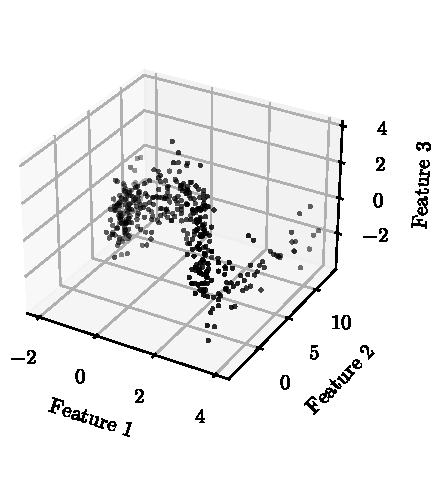
\includegraphics[width=\textwidth]{images/MachineLearning/LinearRegressiondData.pdf}
        \caption{400 data points}
        \label{fig:LinearRegressiondData}
    \end{subfigure}
    \begin{subfigure}{0.49\textwidth}  % <----
        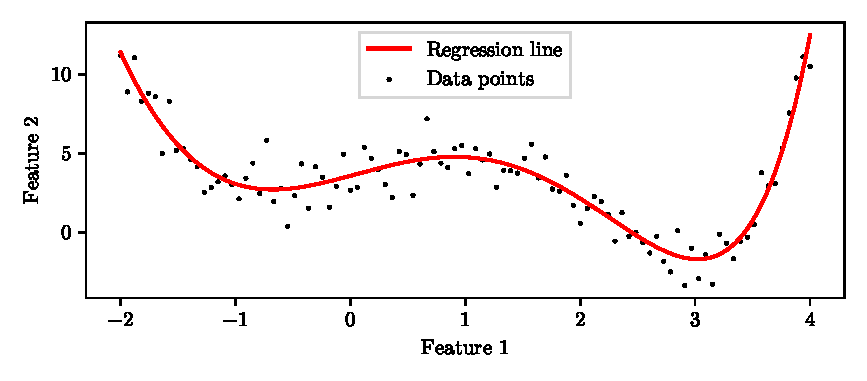
\includegraphics[width=\textwidth]{images/MachineLearning/LinearRegression.pdf}
        \caption{data points and the fitted curve}
        \label{fig:LinearRegression}
    \end{subfigure}
    \caption{Least square regression example}
\end{figure}

rearranging in matrix form: 
\begin{equation}
    \underbrace{\begin{bmatrix}
        y_{1,1} & y_{1,2} \\
        y_{2,1} & y_{2,2} \\
        \vdots & \vdots \\
        y_{m,1} & y_{m,2} \\
    \end{bmatrix}}_{\vect{Y}}
    =
    \underbrace{\begin{bmatrix}
        e^{x_1} & x_1^3 & \cos(x_1) & \sin(x_1) & \cos^3(x_1) \\
        e^{x_2} & x_2^3 & \cos(x_2) & \sin(x_2) & \cos^3(x_2) \\
        \vdots & \vdots & \vdots & \vdots & \vdots \\
        e^{x_m} & x_m^3 & \cos(x_m) & \sin(x_m) & \cos^3(x_m) \\
    \end{bmatrix}}_{\vect{\Phi}(\vect{X})}
    \cdot
    \underbrace{\begin{bmatrix}
        \theta_{1,1}  & \theta_{1,2} \\
        \theta_{2,1}  & \theta_{2,2} \\
        \theta_{3,1}  & \theta_{3,2} \\
        \theta_{4,1}  & \theta_{4,2} \\
        \theta_{5,1}  & \theta_{5,2} \\
    \end{bmatrix}}_{\vect{\Theta}}
\end{equation}

applying the \gls{ls} solution from \autoref{eq:LS}, we obtain:
\begin{equation*}
    \vect{\Theta_{LS}} = \text{pinv}(\vect{\Phi}(\vect{X}))\vect{Y} = 
    \begin{bmatrix}
        +1.997 & -0.004 \\
        -1.498 & +0.003 \\
        +1.332 & -0.018 \\
        -0.005 &  +0.999 \\
        -0.032 & +1.035 
    \end{bmatrix}
\end{equation*}

that is quite close to the real parameters used to generate the data:
\begin{equation*}
    \vect{\Theta}_{\text{true}} = 
    \begin{bmatrix}
        +2.0 & +0 \\
        -1.5 & +0 \\
        +1.3 & +0 \\
        +0.0 & +1 \\
        +0.0 & +1 
    \end{bmatrix}
\end{equation*}

Using the estimated parameters, it is possible to estimate the output features for new input features, the regression line is shown in \autoref{fig:LinearRegression}.

\subsubsection{Applicability}
This is an elegant closed-form solution for a regression problem, however, it has some limitations:
\begin{itemize}
    \item if the noise is not white, or it is present also in the input features, the solution is not guaranteed to converge to the real parameters;
    \item if there are nonlinearities in the parameters (for example $\sin(\theta_{1,1}x)$), the solution is not applicable;
\end{itemize}

\subsection{Gradient Descent \gls{gd}}
To overcome these limitations, another way to estimate the parameters is to use an iterative algorithm that minimizes a cost function over the parameters space. The iterations aim to update the parameters in the direction of the steepest descent of the cost function. This can be done even with nonlinearities in the data, and even if the noise is not white, but has the drawback of the risk of getting stuck in a local minimum of the cost function, starting from a random initialization.
Another limitation is the fact that a learning rate $\eta$ has to be defined, that is a parameter that defines how much the parameters are updated at each iteration. If the learning rate is too small, the algorithm will take a lot of time to converge, if it is too large, the algorithm may overshoot the minimum and avoid convergence.

In the previous closed form solution (\autoref{subsec:LS}), the hypotesis function was linear in the parameters $\vect{Y} = \vect{\Phi}(\vect{X})\cdot\vect{\Theta}$, so we can call this prediction $\vect{\hat{y}} = \vect{h}_{\vect{\Theta}}(\vect{x})$.

The cost function to be minimized is usually defined as the mean squared error between the prediction and the real data:
\begin{equation}
    \text{MSE}(\vect{X}, h_{\vect{\Theta}}) = \frac{1}{m}\sum_{i=1}^{m}(\vect{\hat{y}}_i - \vect{y}_i)^2
\end{equation}


The gradient of the cost function, used by all gradient descent algorithms, is defined as:

\begin{equation}
\nabla_{\vect{\Theta}} \text{MSE}(\vect{X}, h_{\vect{\Theta}}) = 
\begin{bmatrix}
    \frac{\partial}{\partial \theta_1} \text{MSE}(\vect{X}, h_{\vect{\Theta}}) \\
    \frac{\partial}{\partial \theta_2} \text{MSE}(\vect{X}, h_{\vect{\Theta}}) \\
    \vdots \\
    \frac{\partial}{\partial \theta_{n_f\times n_y}} \text{MSE}(\vect{X}, h_{\vect{\Theta}}) \\
\end{bmatrix}
\end{equation}

The algorithm then updates the parameters at each iteration as:
\begin{equation}
    \vect{\Theta}^{(i+1)} = \vect{\Theta}^{(i)} - \eta \nabla_{\vect{\Theta}} \text{MSE}(\vect{X}, h_{\vect{\Theta}})
\end{equation}


\subsection{Sthocastic Gradient Descent}
\label{subsec:SGD}
The \emph{Stochastic Gradient Descent} (\gls{gd}) is a variant of the \gls{gd} algorithm that computes the gradient only on one instance at each iteration, instead of on the whole dataset. This makes the algorithm much faster, but the cost function will be much more noisy, and theta will not reach a steady value but instead will oscillate around the minimum. This has the advantage of being more robust to local minimum entrapment, but the disadvantage of never reaching the minimum. To overcome this, the learning rate $\eta$ can be reduced at each iteration, but this will slow down the convergence.

\begin{figure}
    \centering
    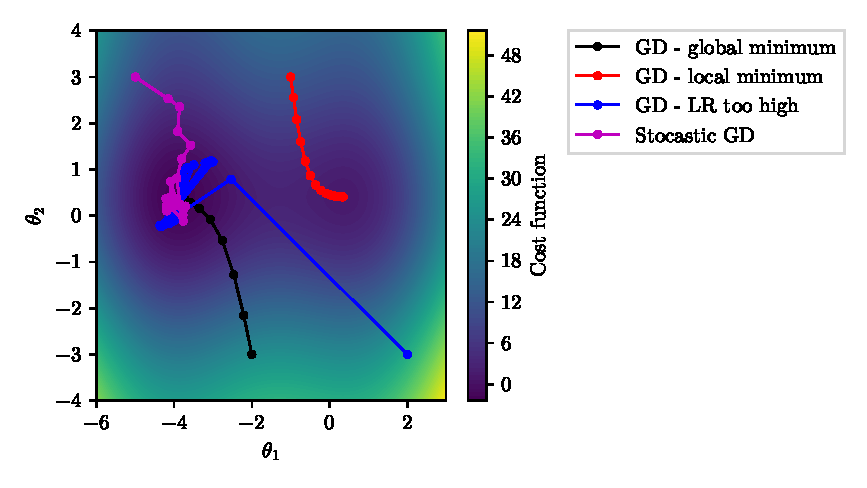
\includegraphics[width=\textwidth]{images/MachineLearning/GradientDescent.pdf}
    \caption{Gradient Descent comparison}
    \label{fig:SGD}
\end{figure}

In the \autoref{fig:SGD} it is visualized graphically what has been said about Gradient Descent.

\subsection{Avoid overfitting}
\label{subsec:overfitting}
The \gls{gd} algorithm is very powerful, but it can overfit the data. To avoid that, the problem of when to stop the iterations has to be addressed. A common way to do that is to split the dataset into a training set and a validation set. The training set is used to train the algorithm, and the validation set is used to evaluate the performance of the algorithm on new data. The training is stopped when the performance on the validation set starts to degrade, even if the performance on the training set is still improving. This is called \emph{early stopping}. In the \autoref{fig:overfitting} it is shown an example of early stopping using as metric the \emph{Root Mean Square Error} (RMSE), that is just the square root of MSE, on the validation set.

\begin{figure}
    \centering
    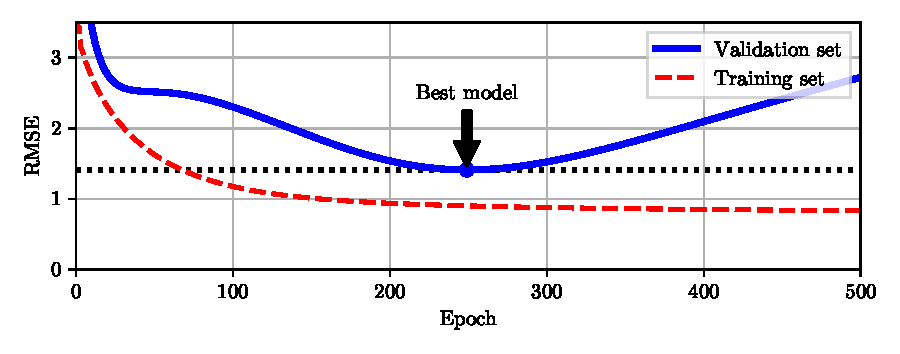
\includegraphics[width=\textwidth]{images/MachineLearning/EarlyStopping.pdf}
    \caption{Overfitting example \citepage{hands-on-geron2022}{162}}
    \label{fig:overfitting}
\end{figure}

\section{Classification}
\label{sec:Classification}
Another common task in \gls{ml} is classification. In this case, the algorithm is trained to assign a label to a new instance, based on the training dataset of labeled instances. Naively, it aims to define a set of rules that divide the space of the input features in regions, each one associated with a label. The two main approaches are \emph{hard} and \emph{soft} classification. In the former, the algorithm is trained to assign a single label to each instance, while in the latter, the algorithm is trained to output a probability for each label, and the label with the highest probability is assigned to the instance.

Classification is a \emph{supervised} learning task because the training dataset is labeled. The labels can be provided by a human or can be generated by another algorithm. Some classification algorithms are available also in the unsupervised version, where the labels are not provided, and the task is usually novelty detection.

\subsection{Support Vector Machines \gls{svm}}
\label{subsec:svm}
Support Vector Machines are simple but powerful classification algorithms that can be used both for hard and soft classification, with medium size datasets. They are based on the idea of finding the hyperplane that best divides the space of the input features into two regions, each one associated with a label.

The main drawback is that, natively, they can only be used for binary classification (two classes), but there are some extensions that allow to use of them for multiclass classification. Furthermore, as will be explained in \autoref{sec:OneClassSupportVectorMachine}, they can be used also for novelty detection (one class). Another limitation is that, being a linear classifier, they can only be used for linearly separable data, but using the \emph{kernel trick}, they can be used also for nonlinearly separable data.

\subsubsection{Linear \gls{svm}}
\label{subsubsec:LinearSVM}

\begin{figure}
    \centering
    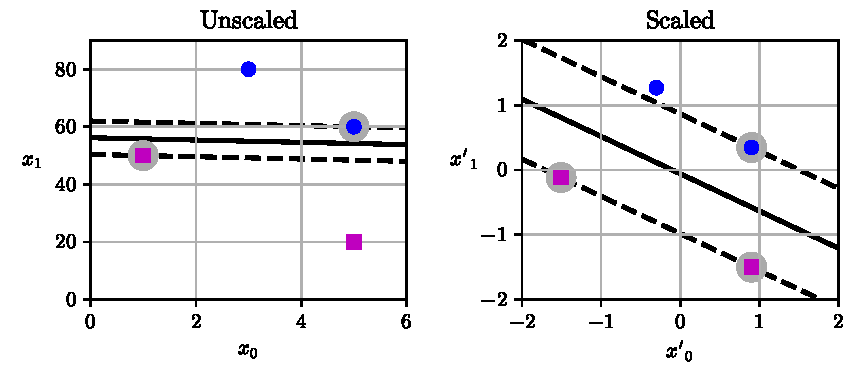
\includegraphics[width=\textwidth]{images/MachineLearning/LinearSVM.pdf}
    \caption{Linear SVM example \citepage{hands-on-geron2022}{176}}
    \label{fig:LinearSVM}
\end{figure}

Looking at \autoref{fig:LinearSVM}, it is possible to visualize what the algorithm does: it finds the plane that separates one class from the other, and vice-versa for the second class. In other words, it finds the most distant parallel hyperplanes that separate the two classes. As evident from the figure, the distance between the hyperplanes (called \emph{margin}) is sensitive to the features scaling. The term \quoted{support} derives from the fact that only the instances that are on the margin, define (support) the two planes. Those instances are called \emph{support vectors}, and in the figure are highlighted with a grey circle.

\subsubsection{Noninear \gls{svm}}
\label{subsubsec:NoninearSVM}
As said before, the \gls{svm} algorithm can be used also for nonlinearly separable data, using the \emph{kernel trick}. The idea is to project the data into a higher dimensional space, where they are linearly separable, and then use the linear \gls{svm} algorithm. The projection is done using a \emph{kernel mapping}. 

Let's have a look at what is the function for classifying an instance $\vect{x}^{(i)}$:
\begin{equation}
    t^{(i)} = \begin{cases}
        -1 & \text{if } \vect{w}^T\vect{x}^{(i)} + b < 0 \\
        1 & \text{if } \vect{w}^T\vect{x}^{(i)} + b \geq 0 
    \end{cases}
\end{equation}

The model is trainded to find the parameters $\vect{w}$ and $b$ that:
\begin{align}
    \label{eq:LinearSVM}
    \underset{\vect{w},b}{\text{minimize }} & \frac{1}{2}\vect{w}^T\vect{w} \\
    \text{subject to } & t^{(i)}(\vect{w}^T\vect{x}^{(i)} + b) \geq 1 \quad \forall i = 1, \dots, m
\end{align}

Since the objective function is convex, and the inequality constraints are differentiable and convex, the solution is the same as the solution of the dual problem \citepage{hands-on-geron2022}{188}:
\begin{align}
    \label{eq:LinearSVMdual}
    \underset{\vect{\alpha}}{\text{minimize }} & \frac{1}{2}\sum_{i=1}^{m}\sum_{j=1}^{m}\alpha^{(i)}\alpha^{(j)}t^{(i)}t^{(j)}\vect{x}^{(i)T}\vect{x}^{(j)} -\sum_{i=1}^{m}\alpha^{(i)}\\
    \text{subject to } & \alpha^{(i)} \geq 0 \quad \forall i = 1, \dots, m \quad \text{and} \quad \sum_{i=1}^{m}\alpha^{(i)}t^{(i)}=0
\end{align}

\paragraph{Kernel Trick}
Suppose wanting to use a second degree polynomial mapping, the mapping function is defined as:
\begin{equation}
    \phi(\vect{x}) = \phi(\begin{bmatrix}
        x_1 \\
        x_2 \\
    \end{bmatrix}) = \begin{bmatrix}
        x_1^2 \\
        \sqrt{2}x_1x_2 \\
        x_2^2 \\
    \end{bmatrix}
\end{equation}

Trasforming two vectors $\vect{a}$ and $\vect{b}$ with the mapping function, to be inserted in \autoref{eq:LinearSVMdual}:
\begin{equation}
    \phi(\vect{a})^T\phi(\vect{b}) = \begin{bmatrix}
        a_1^2 \\
        \sqrt{2}a_1a_2 \\
        a_2^2 \\
    \end{bmatrix}^T
    \begin{bmatrix}
        b_1^2 \\
        \sqrt{2}b_1b_2 \\
        b_2^2 \\
    \end{bmatrix} = a_1^2b_1^2 + 2a_1b_1a_2b_2 + a_2^2b_2^2 = (\vect{a}^T\vect{b})^2
\end{equation}

So, trasforming with a polynomial mapping of degree $d$, does not require to compute the mapping function, but just to compute the dot product of the two vectors and elevate it to the degree $d$, in the dual problem. There also are other kind of kernels, resumed in the following:
\begin{align*}
    \text{Linear: } & K(\vect{a}, \vect{b}) = \vect{a}^T\vect{b} \\
    \text{Polynomial: } & K(\vect{a}, \vect{b}) = (\gamma\vect{a}^T\vect{b} + r)^d \\
    \text{Gaussian RBF: } & K(\vect{a}, \vect{b}) = \exp(-\gamma\norm{\vect{a}-\vect{b}}^2) \\
    \text{Sigmoid: } & K(\vect{a}, \vect{b}) = \tanh(\gamma\vect{a}^T\vect{b} + r)
\end{align*}

\begin{figure}
    \centering
    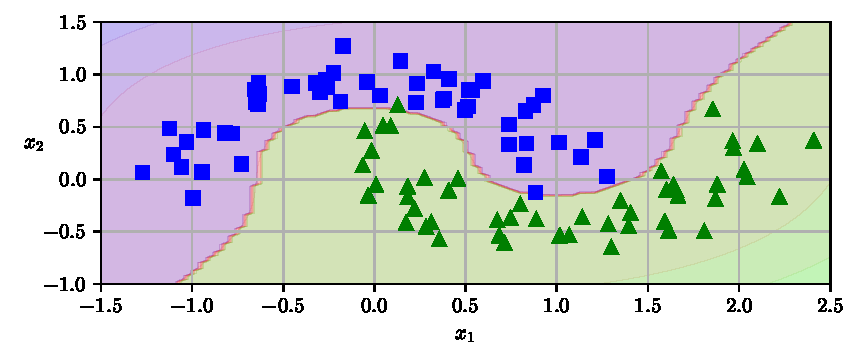
\includegraphics{images/MachineLearning/KernelTrick.pdf}
    \caption{Kernel Trick example \citepage{hands-on-geron2022}{180}}
    \label{fig:KernelTrick}
\end{figure}

The \autoref{fig:KernelTrick} shows an example of \gls{svm} classification of data that are not linearly separable.

This topic seems unrelated to the scope of this thesis, but in \autoref{sec:OneClassSupportVectorMachine} we will see how to use the \gls{svm} algorithm for novelty detection, as a one class classifier.


\subsection{Decision Trees \gls{dt}}
\label{subsec:dt}

\begin{figure}
    \centering
    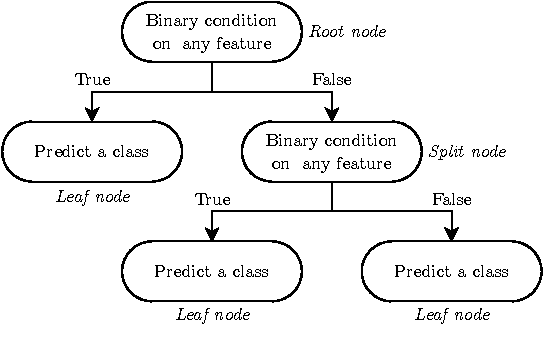
\includegraphics[scale = 1]{images/MachineLearning/DT_structure.pdf}
    \caption{Decision Tree structure}
    \label{fig:DecisionTree}
\end{figure}

Decision Trees are very powerful classification algorithms that can also be used for regression, thinking as a feature values as classes. The classification process is based on a tree structure, where each sample start from the root node, and is filtered thru a bunch of \emph{if - then} statement until it reaches a leaf node, that output the predicited class. In \autoref{fig:DecisionTree}, it is illustrated the structure of a very simple binary tree with only a split node and three leaf nodes.

The classification algorithm is hence very simple, the \gls{ml} part of is the training process. Let's consider a leaf node, and imagine passing all the training samples thru the tree. Ideally, all the samples that reach the leaf node (and any other leaf node) should have the same class. This is possible, but a tree that does that is most likely very overfitted to the train dataset and will not perfom well on future data. Anyway, the aim of training is to obtain a tree close enough to the ideal one, without overfitting. To do that, it exist a metric called \emph{Gini impurity} that assume a value of zero if the leaf node is pure (all the samples that reach it have the same class), or a positive value $\in (0,0.5]$ that measure how different the classes in the node are, 0.5 being the maximum value that mean that all the classes are present in the node with equal frequency. The matematical definition is the following:
\begin{equation}
    G_i = 1 - \sum_{k=1}^{n}p_{i,k}^2
\end{equation}
where $p_{i,k}$ is the ratio of class $k$ instances among the training instances in the $i^{th}$ node.

Then the training procedure tries to grow a tree defining the binary conditions that minimize the weighted average of the Gini impurity of the two child nodes, so the cost function is:
\begin{equation}
    J(k, t_k) = \frac{m_{\text{left}}}{m}G_{\text{left}} + \frac{m_{\text{right}}}{m}G_{\text{right}}
\end{equation}
where $k$ is the feature index, $t_k$ is the threshold value, $m_{\text{left}}$ and $m_{\text{right}}$ are the number of instances in the left and right child nodes, and $G_{\text{left}}$ and $G_{\text{right}}$ are the Gini impurity of the left and right child nodes.

A common way for minimization of the cost function is to use the \emph{Classification and Regression Tree} (\gls{cart}) algorithm, that is a greedy algorithm that search for the optimal split at each node, but not for the global optimal tree. The algorithm complexity is $\mathcal{O}(n \times m \log_2(m))$.

\paragraph{Avoid overfitting}
To avoid overfitting the data, the \gls{cart} algorithm implementation in \texttt{sklearn} has some hyperparameters that can be tuned:
\begin{itemize}
    \item \texttt{max\_depth}: the maximum depth of the tree;
    \item \texttt{min\_samples\_split}: the minimum number of samples a node must have before it can be split;
    \item \texttt{min\_samples\_leaf}: the minimum number of samples a leaf node must have;
    \item \texttt{max\_leaf\_nodes}: the maximum number of leaf nodes;
    \item \texttt{max\_features}: the maximum number of features that are evaluated for splitting at each node.
\end{itemize}
Increasing the \texttt{min} bound, or decreasing the \texttt{max} bound, will regularize the model, and reduce the risk of overfitting.
In \autoref{fig:DecisionTreeOverfitting} it is shown an example of overfitting, where the left plot shows the decision boundaries of a tree with no regularization, and the right plot shows the decision boundaries of a tree with regularization.

\begin{figure}
    \centering
    \scalebox{0.7}{
    %% Creator: Matplotlib, PGF backend
%%
%% To include the figure in your LaTeX document, write
%%   \input{<filename>.pgf}
%%
%% Make sure the required packages are loaded in your preamble
%%   \usepackage{pgf}
%%
%% Also ensure that all the required font packages are loaded; for instance,
%% the lmodern package is sometimes necessary when using math font.
%%   \usepackage{lmodern}
%%
%% Figures using additional raster images can only be included by \input if
%% they are in the same directory as the main LaTeX file. For loading figures
%% from other directories you can use the `import` package
%%   \usepackage{import}
%%
%% and then include the figures with
%%   \import{<path to file>}{<filename>.pgf}
%%
%% Matplotlib used the following preamble
%%   \usepackage{fontspec}
%%   \setmainfont{cmr10.ttf}[Path=\detokenize{C:/ProgramData/Anaconda3/Lib/site-packages/matplotlib/mpl-data/fonts/ttf/}]
%%   \setsansfont{DejaVuSans.ttf}[Path=\detokenize{C:/ProgramData/Anaconda3/Lib/site-packages/matplotlib/mpl-data/fonts/ttf/}]
%%   \setmonofont{DejaVuSansMono.ttf}[Path=\detokenize{C:/ProgramData/Anaconda3/Lib/site-packages/matplotlib/mpl-data/fonts/ttf/}]
%%
\begingroup%
\makeatletter%
\begin{pgfpicture}%
\pgfpathrectangle{\pgfpointorigin}{\pgfqpoint{7.980000in}{3.110000in}}%
\pgfusepath{use as bounding box, clip}%
\begin{pgfscope}%
\pgfsetbuttcap%
\pgfsetmiterjoin%
\definecolor{currentfill}{rgb}{1.000000,1.000000,1.000000}%
\pgfsetfillcolor{currentfill}%
\pgfsetlinewidth{0.000000pt}%
\definecolor{currentstroke}{rgb}{1.000000,1.000000,1.000000}%
\pgfsetstrokecolor{currentstroke}%
\pgfsetdash{}{0pt}%
\pgfpathmoveto{\pgfqpoint{0.000000in}{0.000000in}}%
\pgfpathlineto{\pgfqpoint{7.980000in}{0.000000in}}%
\pgfpathlineto{\pgfqpoint{7.980000in}{3.110000in}}%
\pgfpathlineto{\pgfqpoint{0.000000in}{3.110000in}}%
\pgfpathlineto{\pgfqpoint{0.000000in}{0.000000in}}%
\pgfpathclose%
\pgfusepath{fill}%
\end{pgfscope}%
\begin{pgfscope}%
\pgfsetbuttcap%
\pgfsetmiterjoin%
\definecolor{currentfill}{rgb}{1.000000,1.000000,1.000000}%
\pgfsetfillcolor{currentfill}%
\pgfsetlinewidth{0.000000pt}%
\definecolor{currentstroke}{rgb}{0.000000,0.000000,0.000000}%
\pgfsetstrokecolor{currentstroke}%
\pgfsetstrokeopacity{0.000000}%
\pgfsetdash{}{0pt}%
\pgfpathmoveto{\pgfqpoint{0.997500in}{0.497600in}}%
\pgfpathlineto{\pgfqpoint{3.808636in}{0.497600in}}%
\pgfpathlineto{\pgfqpoint{3.808636in}{2.830100in}}%
\pgfpathlineto{\pgfqpoint{0.997500in}{2.830100in}}%
\pgfpathlineto{\pgfqpoint{0.997500in}{0.497600in}}%
\pgfpathclose%
\pgfusepath{fill}%
\end{pgfscope}%
\begin{pgfscope}%
\pgfpathrectangle{\pgfqpoint{0.997500in}{0.497600in}}{\pgfqpoint{2.811136in}{2.332500in}}%
\pgfusepath{clip}%
\pgfsetbuttcap%
\pgfsetroundjoin%
\definecolor{currentfill}{rgb}{0.924014,0.974533,0.372134}%
\pgfsetfillcolor{currentfill}%
\pgfsetfillopacity{0.300000}%
\pgfsetlinewidth{0.000000pt}%
\definecolor{currentstroke}{rgb}{0.000000,0.000000,0.000000}%
\pgfsetstrokecolor{currentstroke}%
\pgfsetdash{}{0pt}%
\pgfpathmoveto{\pgfqpoint{1.025895in}{0.497600in}}%
\pgfpathlineto{\pgfqpoint{1.054291in}{0.497600in}}%
\pgfpathlineto{\pgfqpoint{1.082686in}{0.497600in}}%
\pgfpathlineto{\pgfqpoint{1.111081in}{0.497600in}}%
\pgfpathlineto{\pgfqpoint{1.139477in}{0.497600in}}%
\pgfpathlineto{\pgfqpoint{1.167872in}{0.497600in}}%
\pgfpathlineto{\pgfqpoint{1.196267in}{0.497600in}}%
\pgfpathlineto{\pgfqpoint{1.224663in}{0.497600in}}%
\pgfpathlineto{\pgfqpoint{1.253058in}{0.497600in}}%
\pgfpathlineto{\pgfqpoint{1.281453in}{0.497600in}}%
\pgfpathlineto{\pgfqpoint{1.309848in}{0.497600in}}%
\pgfpathlineto{\pgfqpoint{1.338244in}{0.497600in}}%
\pgfpathlineto{\pgfqpoint{1.366639in}{0.497600in}}%
\pgfpathlineto{\pgfqpoint{1.395034in}{0.497600in}}%
\pgfpathlineto{\pgfqpoint{1.423430in}{0.497600in}}%
\pgfpathlineto{\pgfqpoint{1.451825in}{0.497600in}}%
\pgfpathlineto{\pgfqpoint{1.480220in}{0.497600in}}%
\pgfpathlineto{\pgfqpoint{1.508616in}{0.497600in}}%
\pgfpathlineto{\pgfqpoint{1.537011in}{0.497600in}}%
\pgfpathlineto{\pgfqpoint{1.565406in}{0.497600in}}%
\pgfpathlineto{\pgfqpoint{1.593802in}{0.497600in}}%
\pgfpathlineto{\pgfqpoint{1.622197in}{0.497600in}}%
\pgfpathlineto{\pgfqpoint{1.650592in}{0.497600in}}%
\pgfpathlineto{\pgfqpoint{1.678988in}{0.497600in}}%
\pgfpathlineto{\pgfqpoint{1.707383in}{0.497600in}}%
\pgfpathlineto{\pgfqpoint{1.735778in}{0.497600in}}%
\pgfpathlineto{\pgfqpoint{1.764174in}{0.497600in}}%
\pgfpathlineto{\pgfqpoint{1.792569in}{0.497600in}}%
\pgfpathlineto{\pgfqpoint{1.820964in}{0.497600in}}%
\pgfpathlineto{\pgfqpoint{1.825223in}{0.497600in}}%
\pgfpathlineto{\pgfqpoint{1.825223in}{0.521161in}}%
\pgfpathlineto{\pgfqpoint{1.825223in}{0.544721in}}%
\pgfpathlineto{\pgfqpoint{1.825223in}{0.568282in}}%
\pgfpathlineto{\pgfqpoint{1.825223in}{0.591842in}}%
\pgfpathlineto{\pgfqpoint{1.825223in}{0.615403in}}%
\pgfpathlineto{\pgfqpoint{1.825223in}{0.638964in}}%
\pgfpathlineto{\pgfqpoint{1.825223in}{0.662524in}}%
\pgfpathlineto{\pgfqpoint{1.825223in}{0.686085in}}%
\pgfpathlineto{\pgfqpoint{1.825223in}{0.709645in}}%
\pgfpathlineto{\pgfqpoint{1.825223in}{0.733206in}}%
\pgfpathlineto{\pgfqpoint{1.825223in}{0.756767in}}%
\pgfpathlineto{\pgfqpoint{1.825223in}{0.780327in}}%
\pgfpathlineto{\pgfqpoint{1.825223in}{0.803888in}}%
\pgfpathlineto{\pgfqpoint{1.825223in}{0.827448in}}%
\pgfpathlineto{\pgfqpoint{1.825223in}{0.851009in}}%
\pgfpathlineto{\pgfqpoint{1.825223in}{0.874570in}}%
\pgfpathlineto{\pgfqpoint{1.825223in}{0.898130in}}%
\pgfpathlineto{\pgfqpoint{1.825223in}{0.921691in}}%
\pgfpathlineto{\pgfqpoint{1.825223in}{0.945252in}}%
\pgfpathlineto{\pgfqpoint{1.825223in}{0.968812in}}%
\pgfpathlineto{\pgfqpoint{1.825223in}{0.992373in}}%
\pgfpathlineto{\pgfqpoint{1.825223in}{1.015933in}}%
\pgfpathlineto{\pgfqpoint{1.825223in}{1.039494in}}%
\pgfpathlineto{\pgfqpoint{1.825223in}{1.063055in}}%
\pgfpathlineto{\pgfqpoint{1.825223in}{1.086615in}}%
\pgfpathlineto{\pgfqpoint{1.825223in}{1.110176in}}%
\pgfpathlineto{\pgfqpoint{1.825223in}{1.133736in}}%
\pgfpathlineto{\pgfqpoint{1.825223in}{1.157297in}}%
\pgfpathlineto{\pgfqpoint{1.825223in}{1.180858in}}%
\pgfpathlineto{\pgfqpoint{1.825223in}{1.204418in}}%
\pgfpathlineto{\pgfqpoint{1.825223in}{1.227979in}}%
\pgfpathlineto{\pgfqpoint{1.825223in}{1.251539in}}%
\pgfpathlineto{\pgfqpoint{1.825223in}{1.275100in}}%
\pgfpathlineto{\pgfqpoint{1.825223in}{1.298661in}}%
\pgfpathlineto{\pgfqpoint{1.825223in}{1.322221in}}%
\pgfpathlineto{\pgfqpoint{1.825223in}{1.345782in}}%
\pgfpathlineto{\pgfqpoint{1.825223in}{1.369342in}}%
\pgfpathlineto{\pgfqpoint{1.825223in}{1.392903in}}%
\pgfpathlineto{\pgfqpoint{1.825223in}{1.416464in}}%
\pgfpathlineto{\pgfqpoint{1.825223in}{1.440024in}}%
\pgfpathlineto{\pgfqpoint{1.849360in}{1.460051in}}%
\pgfpathlineto{\pgfqpoint{1.877755in}{1.460051in}}%
\pgfpathlineto{\pgfqpoint{1.906150in}{1.460051in}}%
\pgfpathlineto{\pgfqpoint{1.934545in}{1.460051in}}%
\pgfpathlineto{\pgfqpoint{1.962941in}{1.460051in}}%
\pgfpathlineto{\pgfqpoint{1.991336in}{1.460051in}}%
\pgfpathlineto{\pgfqpoint{2.019731in}{1.460051in}}%
\pgfpathlineto{\pgfqpoint{2.048127in}{1.460051in}}%
\pgfpathlineto{\pgfqpoint{2.076522in}{1.460051in}}%
\pgfpathlineto{\pgfqpoint{2.104917in}{1.460051in}}%
\pgfpathlineto{\pgfqpoint{2.133313in}{1.460051in}}%
\pgfpathlineto{\pgfqpoint{2.161708in}{1.460051in}}%
\pgfpathlineto{\pgfqpoint{2.190103in}{1.460051in}}%
\pgfpathlineto{\pgfqpoint{2.218499in}{1.460051in}}%
\pgfpathlineto{\pgfqpoint{2.246894in}{1.460051in}}%
\pgfpathlineto{\pgfqpoint{2.275289in}{1.460051in}}%
\pgfpathlineto{\pgfqpoint{2.303685in}{1.460051in}}%
\pgfpathlineto{\pgfqpoint{2.332080in}{1.460051in}}%
\pgfpathlineto{\pgfqpoint{2.360475in}{1.460051in}}%
\pgfpathlineto{\pgfqpoint{2.388871in}{1.460051in}}%
\pgfpathlineto{\pgfqpoint{2.417266in}{1.460051in}}%
\pgfpathlineto{\pgfqpoint{2.445661in}{1.460051in}}%
\pgfpathlineto{\pgfqpoint{2.474056in}{1.460051in}}%
\pgfpathlineto{\pgfqpoint{2.502452in}{1.460051in}}%
\pgfpathlineto{\pgfqpoint{2.530847in}{1.460051in}}%
\pgfpathlineto{\pgfqpoint{2.559242in}{1.460051in}}%
\pgfpathlineto{\pgfqpoint{2.587638in}{1.460051in}}%
\pgfpathlineto{\pgfqpoint{2.611774in}{1.440024in}}%
\pgfpathlineto{\pgfqpoint{2.611774in}{1.416464in}}%
\pgfpathlineto{\pgfqpoint{2.611774in}{1.392903in}}%
\pgfpathlineto{\pgfqpoint{2.616033in}{1.389369in}}%
\pgfpathlineto{\pgfqpoint{2.644428in}{1.389369in}}%
\pgfpathlineto{\pgfqpoint{2.672824in}{1.389369in}}%
\pgfpathlineto{\pgfqpoint{2.701219in}{1.389369in}}%
\pgfpathlineto{\pgfqpoint{2.729614in}{1.389369in}}%
\pgfpathlineto{\pgfqpoint{2.758010in}{1.389369in}}%
\pgfpathlineto{\pgfqpoint{2.786405in}{1.389369in}}%
\pgfpathlineto{\pgfqpoint{2.814800in}{1.389369in}}%
\pgfpathlineto{\pgfqpoint{2.843196in}{1.389369in}}%
\pgfpathlineto{\pgfqpoint{2.871591in}{1.389369in}}%
\pgfpathlineto{\pgfqpoint{2.899986in}{1.389369in}}%
\pgfpathlineto{\pgfqpoint{2.928382in}{1.389369in}}%
\pgfpathlineto{\pgfqpoint{2.956777in}{1.389369in}}%
\pgfpathlineto{\pgfqpoint{2.985172in}{1.389369in}}%
\pgfpathlineto{\pgfqpoint{3.013567in}{1.389369in}}%
\pgfpathlineto{\pgfqpoint{3.041963in}{1.389369in}}%
\pgfpathlineto{\pgfqpoint{3.046222in}{1.392903in}}%
\pgfpathlineto{\pgfqpoint{3.046222in}{1.416464in}}%
\pgfpathlineto{\pgfqpoint{3.046222in}{1.440024in}}%
\pgfpathlineto{\pgfqpoint{3.070358in}{1.460051in}}%
\pgfpathlineto{\pgfqpoint{3.098753in}{1.460051in}}%
\pgfpathlineto{\pgfqpoint{3.127149in}{1.460051in}}%
\pgfpathlineto{\pgfqpoint{3.155544in}{1.460051in}}%
\pgfpathlineto{\pgfqpoint{3.183939in}{1.460051in}}%
\pgfpathlineto{\pgfqpoint{3.212335in}{1.460051in}}%
\pgfpathlineto{\pgfqpoint{3.240730in}{1.460051in}}%
\pgfpathlineto{\pgfqpoint{3.269125in}{1.460051in}}%
\pgfpathlineto{\pgfqpoint{3.297521in}{1.460051in}}%
\pgfpathlineto{\pgfqpoint{3.325916in}{1.460051in}}%
\pgfpathlineto{\pgfqpoint{3.354311in}{1.460051in}}%
\pgfpathlineto{\pgfqpoint{3.382707in}{1.460051in}}%
\pgfpathlineto{\pgfqpoint{3.411102in}{1.460051in}}%
\pgfpathlineto{\pgfqpoint{3.439497in}{1.460051in}}%
\pgfpathlineto{\pgfqpoint{3.467893in}{1.460051in}}%
\pgfpathlineto{\pgfqpoint{3.496288in}{1.460051in}}%
\pgfpathlineto{\pgfqpoint{3.524683in}{1.460051in}}%
\pgfpathlineto{\pgfqpoint{3.553079in}{1.460051in}}%
\pgfpathlineto{\pgfqpoint{3.581474in}{1.460051in}}%
\pgfpathlineto{\pgfqpoint{3.609869in}{1.460051in}}%
\pgfpathlineto{\pgfqpoint{3.638264in}{1.460051in}}%
\pgfpathlineto{\pgfqpoint{3.666660in}{1.460051in}}%
\pgfpathlineto{\pgfqpoint{3.695055in}{1.460051in}}%
\pgfpathlineto{\pgfqpoint{3.723450in}{1.460051in}}%
\pgfpathlineto{\pgfqpoint{3.751846in}{1.460051in}}%
\pgfpathlineto{\pgfqpoint{3.780241in}{1.460051in}}%
\pgfpathlineto{\pgfqpoint{3.808636in}{1.460051in}}%
\pgfpathlineto{\pgfqpoint{3.808636in}{1.463585in}}%
\pgfpathlineto{\pgfqpoint{3.808636in}{1.467119in}}%
\pgfpathlineto{\pgfqpoint{3.780241in}{1.467119in}}%
\pgfpathlineto{\pgfqpoint{3.751846in}{1.467119in}}%
\pgfpathlineto{\pgfqpoint{3.723450in}{1.467119in}}%
\pgfpathlineto{\pgfqpoint{3.695055in}{1.467119in}}%
\pgfpathlineto{\pgfqpoint{3.666660in}{1.467119in}}%
\pgfpathlineto{\pgfqpoint{3.638264in}{1.467119in}}%
\pgfpathlineto{\pgfqpoint{3.609869in}{1.467119in}}%
\pgfpathlineto{\pgfqpoint{3.581474in}{1.467119in}}%
\pgfpathlineto{\pgfqpoint{3.553079in}{1.467119in}}%
\pgfpathlineto{\pgfqpoint{3.524683in}{1.467119in}}%
\pgfpathlineto{\pgfqpoint{3.496288in}{1.467119in}}%
\pgfpathlineto{\pgfqpoint{3.467893in}{1.467119in}}%
\pgfpathlineto{\pgfqpoint{3.439497in}{1.467119in}}%
\pgfpathlineto{\pgfqpoint{3.411102in}{1.467119in}}%
\pgfpathlineto{\pgfqpoint{3.382707in}{1.467119in}}%
\pgfpathlineto{\pgfqpoint{3.354311in}{1.467119in}}%
\pgfpathlineto{\pgfqpoint{3.325916in}{1.467119in}}%
\pgfpathlineto{\pgfqpoint{3.297521in}{1.467119in}}%
\pgfpathlineto{\pgfqpoint{3.269125in}{1.467119in}}%
\pgfpathlineto{\pgfqpoint{3.240730in}{1.467119in}}%
\pgfpathlineto{\pgfqpoint{3.212335in}{1.467119in}}%
\pgfpathlineto{\pgfqpoint{3.183939in}{1.467119in}}%
\pgfpathlineto{\pgfqpoint{3.155544in}{1.467119in}}%
\pgfpathlineto{\pgfqpoint{3.127149in}{1.467119in}}%
\pgfpathlineto{\pgfqpoint{3.098753in}{1.467119in}}%
\pgfpathlineto{\pgfqpoint{3.070358in}{1.467119in}}%
\pgfpathlineto{\pgfqpoint{3.041963in}{1.467119in}}%
\pgfpathlineto{\pgfqpoint{3.013567in}{1.467119in}}%
\pgfpathlineto{\pgfqpoint{2.985172in}{1.467119in}}%
\pgfpathlineto{\pgfqpoint{2.956777in}{1.467119in}}%
\pgfpathlineto{\pgfqpoint{2.928382in}{1.467119in}}%
\pgfpathlineto{\pgfqpoint{2.899986in}{1.467119in}}%
\pgfpathlineto{\pgfqpoint{2.871591in}{1.467119in}}%
\pgfpathlineto{\pgfqpoint{2.843196in}{1.467119in}}%
\pgfpathlineto{\pgfqpoint{2.814800in}{1.467119in}}%
\pgfpathlineto{\pgfqpoint{2.786405in}{1.467119in}}%
\pgfpathlineto{\pgfqpoint{2.758010in}{1.467119in}}%
\pgfpathlineto{\pgfqpoint{2.729614in}{1.467119in}}%
\pgfpathlineto{\pgfqpoint{2.701219in}{1.467119in}}%
\pgfpathlineto{\pgfqpoint{2.672824in}{1.467119in}}%
\pgfpathlineto{\pgfqpoint{2.644428in}{1.467119in}}%
\pgfpathlineto{\pgfqpoint{2.616033in}{1.467119in}}%
\pgfpathlineto{\pgfqpoint{2.587638in}{1.467119in}}%
\pgfpathlineto{\pgfqpoint{2.559242in}{1.467119in}}%
\pgfpathlineto{\pgfqpoint{2.530847in}{1.467119in}}%
\pgfpathlineto{\pgfqpoint{2.502452in}{1.467119in}}%
\pgfpathlineto{\pgfqpoint{2.474056in}{1.467119in}}%
\pgfpathlineto{\pgfqpoint{2.445661in}{1.467119in}}%
\pgfpathlineto{\pgfqpoint{2.417266in}{1.467119in}}%
\pgfpathlineto{\pgfqpoint{2.388871in}{1.467119in}}%
\pgfpathlineto{\pgfqpoint{2.360475in}{1.467119in}}%
\pgfpathlineto{\pgfqpoint{2.332080in}{1.467119in}}%
\pgfpathlineto{\pgfqpoint{2.303685in}{1.467119in}}%
\pgfpathlineto{\pgfqpoint{2.275289in}{1.467119in}}%
\pgfpathlineto{\pgfqpoint{2.246894in}{1.467119in}}%
\pgfpathlineto{\pgfqpoint{2.218499in}{1.467119in}}%
\pgfpathlineto{\pgfqpoint{2.190103in}{1.467119in}}%
\pgfpathlineto{\pgfqpoint{2.161708in}{1.467119in}}%
\pgfpathlineto{\pgfqpoint{2.133313in}{1.467119in}}%
\pgfpathlineto{\pgfqpoint{2.104917in}{1.467119in}}%
\pgfpathlineto{\pgfqpoint{2.076522in}{1.467119in}}%
\pgfpathlineto{\pgfqpoint{2.048127in}{1.467119in}}%
\pgfpathlineto{\pgfqpoint{2.019731in}{1.467119in}}%
\pgfpathlineto{\pgfqpoint{1.991336in}{1.467119in}}%
\pgfpathlineto{\pgfqpoint{1.962941in}{1.467119in}}%
\pgfpathlineto{\pgfqpoint{1.934545in}{1.467119in}}%
\pgfpathlineto{\pgfqpoint{1.906150in}{1.467119in}}%
\pgfpathlineto{\pgfqpoint{1.877755in}{1.467119in}}%
\pgfpathlineto{\pgfqpoint{1.849360in}{1.467119in}}%
\pgfpathlineto{\pgfqpoint{1.825223in}{1.487145in}}%
\pgfpathlineto{\pgfqpoint{1.825223in}{1.510706in}}%
\pgfpathlineto{\pgfqpoint{1.825223in}{1.534267in}}%
\pgfpathlineto{\pgfqpoint{1.825223in}{1.557827in}}%
\pgfpathlineto{\pgfqpoint{1.820964in}{1.561361in}}%
\pgfpathlineto{\pgfqpoint{1.792569in}{1.561361in}}%
\pgfpathlineto{\pgfqpoint{1.764174in}{1.561361in}}%
\pgfpathlineto{\pgfqpoint{1.735778in}{1.561361in}}%
\pgfpathlineto{\pgfqpoint{1.711642in}{1.581388in}}%
\pgfpathlineto{\pgfqpoint{1.711642in}{1.604948in}}%
\pgfpathlineto{\pgfqpoint{1.711642in}{1.628509in}}%
\pgfpathlineto{\pgfqpoint{1.711642in}{1.652070in}}%
\pgfpathlineto{\pgfqpoint{1.711642in}{1.675630in}}%
\pgfpathlineto{\pgfqpoint{1.711642in}{1.699191in}}%
\pgfpathlineto{\pgfqpoint{1.711642in}{1.722752in}}%
\pgfpathlineto{\pgfqpoint{1.711642in}{1.746312in}}%
\pgfpathlineto{\pgfqpoint{1.711642in}{1.769873in}}%
\pgfpathlineto{\pgfqpoint{1.735778in}{1.789899in}}%
\pgfpathlineto{\pgfqpoint{1.764174in}{1.789899in}}%
\pgfpathlineto{\pgfqpoint{1.792569in}{1.789899in}}%
\pgfpathlineto{\pgfqpoint{1.820964in}{1.789899in}}%
\pgfpathlineto{\pgfqpoint{1.849360in}{1.789899in}}%
\pgfpathlineto{\pgfqpoint{1.877755in}{1.789899in}}%
\pgfpathlineto{\pgfqpoint{1.906150in}{1.789899in}}%
\pgfpathlineto{\pgfqpoint{1.934545in}{1.789899in}}%
\pgfpathlineto{\pgfqpoint{1.962941in}{1.789899in}}%
\pgfpathlineto{\pgfqpoint{1.991336in}{1.789899in}}%
\pgfpathlineto{\pgfqpoint{2.019731in}{1.789899in}}%
\pgfpathlineto{\pgfqpoint{2.048127in}{1.789899in}}%
\pgfpathlineto{\pgfqpoint{2.076522in}{1.789899in}}%
\pgfpathlineto{\pgfqpoint{2.104917in}{1.789899in}}%
\pgfpathlineto{\pgfqpoint{2.133313in}{1.789899in}}%
\pgfpathlineto{\pgfqpoint{2.161708in}{1.789899in}}%
\pgfpathlineto{\pgfqpoint{2.190103in}{1.789899in}}%
\pgfpathlineto{\pgfqpoint{2.218499in}{1.789899in}}%
\pgfpathlineto{\pgfqpoint{2.246894in}{1.789899in}}%
\pgfpathlineto{\pgfqpoint{2.275289in}{1.789899in}}%
\pgfpathlineto{\pgfqpoint{2.303685in}{1.789899in}}%
\pgfpathlineto{\pgfqpoint{2.332080in}{1.789899in}}%
\pgfpathlineto{\pgfqpoint{2.360475in}{1.789899in}}%
\pgfpathlineto{\pgfqpoint{2.388871in}{1.789899in}}%
\pgfpathlineto{\pgfqpoint{2.417266in}{1.789899in}}%
\pgfpathlineto{\pgfqpoint{2.445661in}{1.789899in}}%
\pgfpathlineto{\pgfqpoint{2.474056in}{1.789899in}}%
\pgfpathlineto{\pgfqpoint{2.502452in}{1.789899in}}%
\pgfpathlineto{\pgfqpoint{2.530847in}{1.789899in}}%
\pgfpathlineto{\pgfqpoint{2.559242in}{1.789899in}}%
\pgfpathlineto{\pgfqpoint{2.587638in}{1.789899in}}%
\pgfpathlineto{\pgfqpoint{2.616033in}{1.789899in}}%
\pgfpathlineto{\pgfqpoint{2.640169in}{1.769873in}}%
\pgfpathlineto{\pgfqpoint{2.640169in}{1.746312in}}%
\pgfpathlineto{\pgfqpoint{2.640169in}{1.722752in}}%
\pgfpathlineto{\pgfqpoint{2.640169in}{1.699191in}}%
\pgfpathlineto{\pgfqpoint{2.640169in}{1.675630in}}%
\pgfpathlineto{\pgfqpoint{2.640169in}{1.652070in}}%
\pgfpathlineto{\pgfqpoint{2.640169in}{1.628509in}}%
\pgfpathlineto{\pgfqpoint{2.640169in}{1.604948in}}%
\pgfpathlineto{\pgfqpoint{2.640169in}{1.581388in}}%
\pgfpathlineto{\pgfqpoint{2.644428in}{1.577854in}}%
\pgfpathlineto{\pgfqpoint{2.672824in}{1.577854in}}%
\pgfpathlineto{\pgfqpoint{2.701219in}{1.577854in}}%
\pgfpathlineto{\pgfqpoint{2.729614in}{1.577854in}}%
\pgfpathlineto{\pgfqpoint{2.758010in}{1.577854in}}%
\pgfpathlineto{\pgfqpoint{2.786405in}{1.577854in}}%
\pgfpathlineto{\pgfqpoint{2.814800in}{1.577854in}}%
\pgfpathlineto{\pgfqpoint{2.843196in}{1.577854in}}%
\pgfpathlineto{\pgfqpoint{2.871591in}{1.577854in}}%
\pgfpathlineto{\pgfqpoint{2.899986in}{1.577854in}}%
\pgfpathlineto{\pgfqpoint{2.928382in}{1.577854in}}%
\pgfpathlineto{\pgfqpoint{2.956777in}{1.577854in}}%
\pgfpathlineto{\pgfqpoint{2.985172in}{1.577854in}}%
\pgfpathlineto{\pgfqpoint{3.013567in}{1.577854in}}%
\pgfpathlineto{\pgfqpoint{3.041963in}{1.577854in}}%
\pgfpathlineto{\pgfqpoint{3.070358in}{1.577854in}}%
\pgfpathlineto{\pgfqpoint{3.098753in}{1.577854in}}%
\pgfpathlineto{\pgfqpoint{3.127149in}{1.577854in}}%
\pgfpathlineto{\pgfqpoint{3.155544in}{1.577854in}}%
\pgfpathlineto{\pgfqpoint{3.159803in}{1.581388in}}%
\pgfpathlineto{\pgfqpoint{3.159803in}{1.604948in}}%
\pgfpathlineto{\pgfqpoint{3.159803in}{1.628509in}}%
\pgfpathlineto{\pgfqpoint{3.159803in}{1.652070in}}%
\pgfpathlineto{\pgfqpoint{3.159803in}{1.675630in}}%
\pgfpathlineto{\pgfqpoint{3.159803in}{1.699191in}}%
\pgfpathlineto{\pgfqpoint{3.159803in}{1.722752in}}%
\pgfpathlineto{\pgfqpoint{3.159803in}{1.746312in}}%
\pgfpathlineto{\pgfqpoint{3.159803in}{1.769873in}}%
\pgfpathlineto{\pgfqpoint{3.159803in}{1.793433in}}%
\pgfpathlineto{\pgfqpoint{3.159803in}{1.816994in}}%
\pgfpathlineto{\pgfqpoint{3.159803in}{1.840555in}}%
\pgfpathlineto{\pgfqpoint{3.159803in}{1.864115in}}%
\pgfpathlineto{\pgfqpoint{3.159803in}{1.887676in}}%
\pgfpathlineto{\pgfqpoint{3.155544in}{1.891210in}}%
\pgfpathlineto{\pgfqpoint{3.127149in}{1.891210in}}%
\pgfpathlineto{\pgfqpoint{3.098753in}{1.891210in}}%
\pgfpathlineto{\pgfqpoint{3.070358in}{1.891210in}}%
\pgfpathlineto{\pgfqpoint{3.041963in}{1.891210in}}%
\pgfpathlineto{\pgfqpoint{3.013567in}{1.891210in}}%
\pgfpathlineto{\pgfqpoint{2.985172in}{1.891210in}}%
\pgfpathlineto{\pgfqpoint{2.956777in}{1.891210in}}%
\pgfpathlineto{\pgfqpoint{2.928382in}{1.891210in}}%
\pgfpathlineto{\pgfqpoint{2.899986in}{1.891210in}}%
\pgfpathlineto{\pgfqpoint{2.871591in}{1.891210in}}%
\pgfpathlineto{\pgfqpoint{2.843196in}{1.891210in}}%
\pgfpathlineto{\pgfqpoint{2.814800in}{1.891210in}}%
\pgfpathlineto{\pgfqpoint{2.786405in}{1.891210in}}%
\pgfpathlineto{\pgfqpoint{2.758010in}{1.891210in}}%
\pgfpathlineto{\pgfqpoint{2.729614in}{1.891210in}}%
\pgfpathlineto{\pgfqpoint{2.701219in}{1.891210in}}%
\pgfpathlineto{\pgfqpoint{2.672824in}{1.891210in}}%
\pgfpathlineto{\pgfqpoint{2.644428in}{1.891210in}}%
\pgfpathlineto{\pgfqpoint{2.616033in}{1.891210in}}%
\pgfpathlineto{\pgfqpoint{2.587638in}{1.891210in}}%
\pgfpathlineto{\pgfqpoint{2.559242in}{1.891210in}}%
\pgfpathlineto{\pgfqpoint{2.530847in}{1.891210in}}%
\pgfpathlineto{\pgfqpoint{2.502452in}{1.891210in}}%
\pgfpathlineto{\pgfqpoint{2.474056in}{1.891210in}}%
\pgfpathlineto{\pgfqpoint{2.445661in}{1.891210in}}%
\pgfpathlineto{\pgfqpoint{2.417266in}{1.891210in}}%
\pgfpathlineto{\pgfqpoint{2.388871in}{1.891210in}}%
\pgfpathlineto{\pgfqpoint{2.360475in}{1.891210in}}%
\pgfpathlineto{\pgfqpoint{2.332080in}{1.891210in}}%
\pgfpathlineto{\pgfqpoint{2.303685in}{1.891210in}}%
\pgfpathlineto{\pgfqpoint{2.275289in}{1.891210in}}%
\pgfpathlineto{\pgfqpoint{2.246894in}{1.891210in}}%
\pgfpathlineto{\pgfqpoint{2.218499in}{1.891210in}}%
\pgfpathlineto{\pgfqpoint{2.190103in}{1.891210in}}%
\pgfpathlineto{\pgfqpoint{2.161708in}{1.891210in}}%
\pgfpathlineto{\pgfqpoint{2.133313in}{1.891210in}}%
\pgfpathlineto{\pgfqpoint{2.104917in}{1.891210in}}%
\pgfpathlineto{\pgfqpoint{2.076522in}{1.891210in}}%
\pgfpathlineto{\pgfqpoint{2.048127in}{1.891210in}}%
\pgfpathlineto{\pgfqpoint{2.019731in}{1.891210in}}%
\pgfpathlineto{\pgfqpoint{1.991336in}{1.891210in}}%
\pgfpathlineto{\pgfqpoint{1.962941in}{1.891210in}}%
\pgfpathlineto{\pgfqpoint{1.934545in}{1.891210in}}%
\pgfpathlineto{\pgfqpoint{1.906150in}{1.891210in}}%
\pgfpathlineto{\pgfqpoint{1.877755in}{1.891210in}}%
\pgfpathlineto{\pgfqpoint{1.849360in}{1.891210in}}%
\pgfpathlineto{\pgfqpoint{1.820964in}{1.891210in}}%
\pgfpathlineto{\pgfqpoint{1.792569in}{1.891210in}}%
\pgfpathlineto{\pgfqpoint{1.764174in}{1.891210in}}%
\pgfpathlineto{\pgfqpoint{1.735778in}{1.891210in}}%
\pgfpathlineto{\pgfqpoint{1.707383in}{1.891210in}}%
\pgfpathlineto{\pgfqpoint{1.678988in}{1.891210in}}%
\pgfpathlineto{\pgfqpoint{1.650592in}{1.891210in}}%
\pgfpathlineto{\pgfqpoint{1.622197in}{1.891210in}}%
\pgfpathlineto{\pgfqpoint{1.593802in}{1.891210in}}%
\pgfpathlineto{\pgfqpoint{1.565406in}{1.891210in}}%
\pgfpathlineto{\pgfqpoint{1.537011in}{1.891210in}}%
\pgfpathlineto{\pgfqpoint{1.508616in}{1.891210in}}%
\pgfpathlineto{\pgfqpoint{1.480220in}{1.891210in}}%
\pgfpathlineto{\pgfqpoint{1.451825in}{1.891210in}}%
\pgfpathlineto{\pgfqpoint{1.423430in}{1.891210in}}%
\pgfpathlineto{\pgfqpoint{1.395034in}{1.891210in}}%
\pgfpathlineto{\pgfqpoint{1.366639in}{1.891210in}}%
\pgfpathlineto{\pgfqpoint{1.338244in}{1.891210in}}%
\pgfpathlineto{\pgfqpoint{1.309848in}{1.891210in}}%
\pgfpathlineto{\pgfqpoint{1.281453in}{1.891210in}}%
\pgfpathlineto{\pgfqpoint{1.253058in}{1.891210in}}%
\pgfpathlineto{\pgfqpoint{1.224663in}{1.891210in}}%
\pgfpathlineto{\pgfqpoint{1.196267in}{1.891210in}}%
\pgfpathlineto{\pgfqpoint{1.167872in}{1.891210in}}%
\pgfpathlineto{\pgfqpoint{1.139477in}{1.891210in}}%
\pgfpathlineto{\pgfqpoint{1.111081in}{1.891210in}}%
\pgfpathlineto{\pgfqpoint{1.082686in}{1.891210in}}%
\pgfpathlineto{\pgfqpoint{1.054291in}{1.891210in}}%
\pgfpathlineto{\pgfqpoint{1.025895in}{1.891210in}}%
\pgfpathlineto{\pgfqpoint{0.997500in}{1.891210in}}%
\pgfpathlineto{\pgfqpoint{0.997500in}{1.887676in}}%
\pgfpathlineto{\pgfqpoint{0.997500in}{1.864115in}}%
\pgfpathlineto{\pgfqpoint{0.997500in}{1.840555in}}%
\pgfpathlineto{\pgfqpoint{0.997500in}{1.816994in}}%
\pgfpathlineto{\pgfqpoint{0.997500in}{1.793433in}}%
\pgfpathlineto{\pgfqpoint{0.997500in}{1.769873in}}%
\pgfpathlineto{\pgfqpoint{0.997500in}{1.746312in}}%
\pgfpathlineto{\pgfqpoint{0.997500in}{1.722752in}}%
\pgfpathlineto{\pgfqpoint{0.997500in}{1.699191in}}%
\pgfpathlineto{\pgfqpoint{0.997500in}{1.675630in}}%
\pgfpathlineto{\pgfqpoint{0.997500in}{1.652070in}}%
\pgfpathlineto{\pgfqpoint{0.997500in}{1.628509in}}%
\pgfpathlineto{\pgfqpoint{0.997500in}{1.604948in}}%
\pgfpathlineto{\pgfqpoint{0.997500in}{1.581388in}}%
\pgfpathlineto{\pgfqpoint{0.997500in}{1.557827in}}%
\pgfpathlineto{\pgfqpoint{0.997500in}{1.534267in}}%
\pgfpathlineto{\pgfqpoint{0.997500in}{1.510706in}}%
\pgfpathlineto{\pgfqpoint{0.997500in}{1.487145in}}%
\pgfpathlineto{\pgfqpoint{0.997500in}{1.463585in}}%
\pgfpathlineto{\pgfqpoint{0.997500in}{1.440024in}}%
\pgfpathlineto{\pgfqpoint{0.997500in}{1.416464in}}%
\pgfpathlineto{\pgfqpoint{0.997500in}{1.392903in}}%
\pgfpathlineto{\pgfqpoint{0.997500in}{1.369342in}}%
\pgfpathlineto{\pgfqpoint{0.997500in}{1.345782in}}%
\pgfpathlineto{\pgfqpoint{0.997500in}{1.322221in}}%
\pgfpathlineto{\pgfqpoint{0.997500in}{1.298661in}}%
\pgfpathlineto{\pgfqpoint{0.997500in}{1.275100in}}%
\pgfpathlineto{\pgfqpoint{0.997500in}{1.251539in}}%
\pgfpathlineto{\pgfqpoint{0.997500in}{1.227979in}}%
\pgfpathlineto{\pgfqpoint{0.997500in}{1.204418in}}%
\pgfpathlineto{\pgfqpoint{0.997500in}{1.180858in}}%
\pgfpathlineto{\pgfqpoint{0.997500in}{1.157297in}}%
\pgfpathlineto{\pgfqpoint{0.997500in}{1.133736in}}%
\pgfpathlineto{\pgfqpoint{0.997500in}{1.110176in}}%
\pgfpathlineto{\pgfqpoint{0.997500in}{1.086615in}}%
\pgfpathlineto{\pgfqpoint{0.997500in}{1.063055in}}%
\pgfpathlineto{\pgfqpoint{0.997500in}{1.039494in}}%
\pgfpathlineto{\pgfqpoint{0.997500in}{1.015933in}}%
\pgfpathlineto{\pgfqpoint{0.997500in}{0.992373in}}%
\pgfpathlineto{\pgfqpoint{0.997500in}{0.968812in}}%
\pgfpathlineto{\pgfqpoint{0.997500in}{0.945252in}}%
\pgfpathlineto{\pgfqpoint{0.997500in}{0.921691in}}%
\pgfpathlineto{\pgfqpoint{0.997500in}{0.898130in}}%
\pgfpathlineto{\pgfqpoint{0.997500in}{0.874570in}}%
\pgfpathlineto{\pgfqpoint{0.997500in}{0.851009in}}%
\pgfpathlineto{\pgfqpoint{0.997500in}{0.827448in}}%
\pgfpathlineto{\pgfqpoint{0.997500in}{0.803888in}}%
\pgfpathlineto{\pgfqpoint{0.997500in}{0.780327in}}%
\pgfpathlineto{\pgfqpoint{0.997500in}{0.756767in}}%
\pgfpathlineto{\pgfqpoint{0.997500in}{0.733206in}}%
\pgfpathlineto{\pgfqpoint{0.997500in}{0.709645in}}%
\pgfpathlineto{\pgfqpoint{0.997500in}{0.686085in}}%
\pgfpathlineto{\pgfqpoint{0.997500in}{0.662524in}}%
\pgfpathlineto{\pgfqpoint{0.997500in}{0.638964in}}%
\pgfpathlineto{\pgfqpoint{0.997500in}{0.615403in}}%
\pgfpathlineto{\pgfqpoint{0.997500in}{0.591842in}}%
\pgfpathlineto{\pgfqpoint{0.997500in}{0.568282in}}%
\pgfpathlineto{\pgfqpoint{0.997500in}{0.544721in}}%
\pgfpathlineto{\pgfqpoint{0.997500in}{0.521161in}}%
\pgfpathlineto{\pgfqpoint{0.997500in}{0.497600in}}%
\pgfpathlineto{\pgfqpoint{1.025895in}{0.497600in}}%
\pgfpathclose%
\pgfusepath{fill}%
\end{pgfscope}%
\begin{pgfscope}%
\pgfpathrectangle{\pgfqpoint{0.997500in}{0.497600in}}{\pgfqpoint{2.811136in}{2.332500in}}%
\pgfusepath{clip}%
\pgfsetbuttcap%
\pgfsetroundjoin%
\definecolor{currentfill}{rgb}{0.924014,0.974533,0.372134}%
\pgfsetfillcolor{currentfill}%
\pgfsetfillopacity{0.300000}%
\pgfsetlinewidth{0.000000pt}%
\definecolor{currentstroke}{rgb}{0.000000,0.000000,0.000000}%
\pgfsetstrokecolor{currentstroke}%
\pgfsetdash{}{0pt}%
\pgfpathmoveto{\pgfqpoint{1.025895in}{1.931263in}}%
\pgfpathlineto{\pgfqpoint{1.054291in}{1.931263in}}%
\pgfpathlineto{\pgfqpoint{1.082686in}{1.931263in}}%
\pgfpathlineto{\pgfqpoint{1.111081in}{1.931263in}}%
\pgfpathlineto{\pgfqpoint{1.139477in}{1.931263in}}%
\pgfpathlineto{\pgfqpoint{1.167872in}{1.931263in}}%
\pgfpathlineto{\pgfqpoint{1.196267in}{1.931263in}}%
\pgfpathlineto{\pgfqpoint{1.224663in}{1.931263in}}%
\pgfpathlineto{\pgfqpoint{1.253058in}{1.931263in}}%
\pgfpathlineto{\pgfqpoint{1.281453in}{1.931263in}}%
\pgfpathlineto{\pgfqpoint{1.309848in}{1.931263in}}%
\pgfpathlineto{\pgfqpoint{1.338244in}{1.931263in}}%
\pgfpathlineto{\pgfqpoint{1.366639in}{1.931263in}}%
\pgfpathlineto{\pgfqpoint{1.395034in}{1.931263in}}%
\pgfpathlineto{\pgfqpoint{1.423430in}{1.931263in}}%
\pgfpathlineto{\pgfqpoint{1.451825in}{1.931263in}}%
\pgfpathlineto{\pgfqpoint{1.480220in}{1.931263in}}%
\pgfpathlineto{\pgfqpoint{1.508616in}{1.931263in}}%
\pgfpathlineto{\pgfqpoint{1.537011in}{1.931263in}}%
\pgfpathlineto{\pgfqpoint{1.565406in}{1.931263in}}%
\pgfpathlineto{\pgfqpoint{1.593802in}{1.931263in}}%
\pgfpathlineto{\pgfqpoint{1.622197in}{1.931263in}}%
\pgfpathlineto{\pgfqpoint{1.650592in}{1.931263in}}%
\pgfpathlineto{\pgfqpoint{1.678988in}{1.931263in}}%
\pgfpathlineto{\pgfqpoint{1.707383in}{1.931263in}}%
\pgfpathlineto{\pgfqpoint{1.735778in}{1.931263in}}%
\pgfpathlineto{\pgfqpoint{1.764174in}{1.931263in}}%
\pgfpathlineto{\pgfqpoint{1.792569in}{1.931263in}}%
\pgfpathlineto{\pgfqpoint{1.820964in}{1.931263in}}%
\pgfpathlineto{\pgfqpoint{1.849360in}{1.931263in}}%
\pgfpathlineto{\pgfqpoint{1.877755in}{1.931263in}}%
\pgfpathlineto{\pgfqpoint{1.906150in}{1.931263in}}%
\pgfpathlineto{\pgfqpoint{1.934545in}{1.931263in}}%
\pgfpathlineto{\pgfqpoint{1.962941in}{1.931263in}}%
\pgfpathlineto{\pgfqpoint{1.991336in}{1.931263in}}%
\pgfpathlineto{\pgfqpoint{2.019731in}{1.931263in}}%
\pgfpathlineto{\pgfqpoint{2.048127in}{1.931263in}}%
\pgfpathlineto{\pgfqpoint{2.076522in}{1.931263in}}%
\pgfpathlineto{\pgfqpoint{2.104917in}{1.931263in}}%
\pgfpathlineto{\pgfqpoint{2.133313in}{1.931263in}}%
\pgfpathlineto{\pgfqpoint{2.137572in}{1.934797in}}%
\pgfpathlineto{\pgfqpoint{2.137572in}{1.958358in}}%
\pgfpathlineto{\pgfqpoint{2.137572in}{1.981918in}}%
\pgfpathlineto{\pgfqpoint{2.137572in}{2.005479in}}%
\pgfpathlineto{\pgfqpoint{2.137572in}{2.029039in}}%
\pgfpathlineto{\pgfqpoint{2.137572in}{2.052600in}}%
\pgfpathlineto{\pgfqpoint{2.137572in}{2.076161in}}%
\pgfpathlineto{\pgfqpoint{2.137572in}{2.099721in}}%
\pgfpathlineto{\pgfqpoint{2.133313in}{2.103255in}}%
\pgfpathlineto{\pgfqpoint{2.104917in}{2.103255in}}%
\pgfpathlineto{\pgfqpoint{2.076522in}{2.103255in}}%
\pgfpathlineto{\pgfqpoint{2.048127in}{2.103255in}}%
\pgfpathlineto{\pgfqpoint{2.019731in}{2.103255in}}%
\pgfpathlineto{\pgfqpoint{1.991336in}{2.103255in}}%
\pgfpathlineto{\pgfqpoint{1.962941in}{2.103255in}}%
\pgfpathlineto{\pgfqpoint{1.934545in}{2.103255in}}%
\pgfpathlineto{\pgfqpoint{1.906150in}{2.103255in}}%
\pgfpathlineto{\pgfqpoint{1.877755in}{2.103255in}}%
\pgfpathlineto{\pgfqpoint{1.849360in}{2.103255in}}%
\pgfpathlineto{\pgfqpoint{1.820964in}{2.103255in}}%
\pgfpathlineto{\pgfqpoint{1.792569in}{2.103255in}}%
\pgfpathlineto{\pgfqpoint{1.764174in}{2.103255in}}%
\pgfpathlineto{\pgfqpoint{1.735778in}{2.103255in}}%
\pgfpathlineto{\pgfqpoint{1.707383in}{2.103255in}}%
\pgfpathlineto{\pgfqpoint{1.678988in}{2.103255in}}%
\pgfpathlineto{\pgfqpoint{1.650592in}{2.103255in}}%
\pgfpathlineto{\pgfqpoint{1.622197in}{2.103255in}}%
\pgfpathlineto{\pgfqpoint{1.593802in}{2.103255in}}%
\pgfpathlineto{\pgfqpoint{1.565406in}{2.103255in}}%
\pgfpathlineto{\pgfqpoint{1.537011in}{2.103255in}}%
\pgfpathlineto{\pgfqpoint{1.508616in}{2.103255in}}%
\pgfpathlineto{\pgfqpoint{1.480220in}{2.103255in}}%
\pgfpathlineto{\pgfqpoint{1.451825in}{2.103255in}}%
\pgfpathlineto{\pgfqpoint{1.423430in}{2.103255in}}%
\pgfpathlineto{\pgfqpoint{1.395034in}{2.103255in}}%
\pgfpathlineto{\pgfqpoint{1.366639in}{2.103255in}}%
\pgfpathlineto{\pgfqpoint{1.338244in}{2.103255in}}%
\pgfpathlineto{\pgfqpoint{1.309848in}{2.103255in}}%
\pgfpathlineto{\pgfqpoint{1.281453in}{2.103255in}}%
\pgfpathlineto{\pgfqpoint{1.253058in}{2.103255in}}%
\pgfpathlineto{\pgfqpoint{1.224663in}{2.103255in}}%
\pgfpathlineto{\pgfqpoint{1.196267in}{2.103255in}}%
\pgfpathlineto{\pgfqpoint{1.167872in}{2.103255in}}%
\pgfpathlineto{\pgfqpoint{1.139477in}{2.103255in}}%
\pgfpathlineto{\pgfqpoint{1.111081in}{2.103255in}}%
\pgfpathlineto{\pgfqpoint{1.082686in}{2.103255in}}%
\pgfpathlineto{\pgfqpoint{1.054291in}{2.103255in}}%
\pgfpathlineto{\pgfqpoint{1.025895in}{2.103255in}}%
\pgfpathlineto{\pgfqpoint{0.997500in}{2.103255in}}%
\pgfpathlineto{\pgfqpoint{0.997500in}{2.099721in}}%
\pgfpathlineto{\pgfqpoint{0.997500in}{2.076161in}}%
\pgfpathlineto{\pgfqpoint{0.997500in}{2.052600in}}%
\pgfpathlineto{\pgfqpoint{0.997500in}{2.029039in}}%
\pgfpathlineto{\pgfqpoint{0.997500in}{2.005479in}}%
\pgfpathlineto{\pgfqpoint{0.997500in}{1.981918in}}%
\pgfpathlineto{\pgfqpoint{0.997500in}{1.958358in}}%
\pgfpathlineto{\pgfqpoint{0.997500in}{1.934797in}}%
\pgfpathlineto{\pgfqpoint{0.997500in}{1.931263in}}%
\pgfpathlineto{\pgfqpoint{1.025895in}{1.931263in}}%
\pgfpathclose%
\pgfusepath{fill}%
\end{pgfscope}%
\begin{pgfscope}%
\pgfpathrectangle{\pgfqpoint{0.997500in}{0.497600in}}{\pgfqpoint{2.811136in}{2.332500in}}%
\pgfusepath{clip}%
\pgfsetbuttcap%
\pgfsetroundjoin%
\definecolor{currentfill}{rgb}{0.924014,0.974533,0.372134}%
\pgfsetfillcolor{currentfill}%
\pgfsetfillopacity{0.300000}%
\pgfsetlinewidth{0.000000pt}%
\definecolor{currentstroke}{rgb}{0.000000,0.000000,0.000000}%
\pgfsetstrokecolor{currentstroke}%
\pgfsetdash{}{0pt}%
\pgfpathmoveto{\pgfqpoint{2.275289in}{1.931263in}}%
\pgfpathlineto{\pgfqpoint{2.303685in}{1.931263in}}%
\pgfpathlineto{\pgfqpoint{2.332080in}{1.931263in}}%
\pgfpathlineto{\pgfqpoint{2.360475in}{1.931263in}}%
\pgfpathlineto{\pgfqpoint{2.388871in}{1.931263in}}%
\pgfpathlineto{\pgfqpoint{2.417266in}{1.931263in}}%
\pgfpathlineto{\pgfqpoint{2.445661in}{1.931263in}}%
\pgfpathlineto{\pgfqpoint{2.474056in}{1.931263in}}%
\pgfpathlineto{\pgfqpoint{2.502452in}{1.931263in}}%
\pgfpathlineto{\pgfqpoint{2.530847in}{1.931263in}}%
\pgfpathlineto{\pgfqpoint{2.559242in}{1.931263in}}%
\pgfpathlineto{\pgfqpoint{2.587638in}{1.931263in}}%
\pgfpathlineto{\pgfqpoint{2.616033in}{1.931263in}}%
\pgfpathlineto{\pgfqpoint{2.644428in}{1.931263in}}%
\pgfpathlineto{\pgfqpoint{2.672824in}{1.931263in}}%
\pgfpathlineto{\pgfqpoint{2.701219in}{1.931263in}}%
\pgfpathlineto{\pgfqpoint{2.729614in}{1.931263in}}%
\pgfpathlineto{\pgfqpoint{2.758010in}{1.931263in}}%
\pgfpathlineto{\pgfqpoint{2.786405in}{1.931263in}}%
\pgfpathlineto{\pgfqpoint{2.814800in}{1.931263in}}%
\pgfpathlineto{\pgfqpoint{2.843196in}{1.931263in}}%
\pgfpathlineto{\pgfqpoint{2.871591in}{1.931263in}}%
\pgfpathlineto{\pgfqpoint{2.899986in}{1.931263in}}%
\pgfpathlineto{\pgfqpoint{2.928382in}{1.931263in}}%
\pgfpathlineto{\pgfqpoint{2.956777in}{1.931263in}}%
\pgfpathlineto{\pgfqpoint{2.985172in}{1.931263in}}%
\pgfpathlineto{\pgfqpoint{3.013567in}{1.931263in}}%
\pgfpathlineto{\pgfqpoint{3.041963in}{1.931263in}}%
\pgfpathlineto{\pgfqpoint{3.070358in}{1.931263in}}%
\pgfpathlineto{\pgfqpoint{3.098753in}{1.931263in}}%
\pgfpathlineto{\pgfqpoint{3.127149in}{1.931263in}}%
\pgfpathlineto{\pgfqpoint{3.155544in}{1.931263in}}%
\pgfpathlineto{\pgfqpoint{3.159803in}{1.934797in}}%
\pgfpathlineto{\pgfqpoint{3.159803in}{1.958358in}}%
\pgfpathlineto{\pgfqpoint{3.159803in}{1.981918in}}%
\pgfpathlineto{\pgfqpoint{3.159803in}{2.005479in}}%
\pgfpathlineto{\pgfqpoint{3.159803in}{2.029039in}}%
\pgfpathlineto{\pgfqpoint{3.159803in}{2.052600in}}%
\pgfpathlineto{\pgfqpoint{3.159803in}{2.076161in}}%
\pgfpathlineto{\pgfqpoint{3.159803in}{2.099721in}}%
\pgfpathlineto{\pgfqpoint{3.155544in}{2.103255in}}%
\pgfpathlineto{\pgfqpoint{3.127149in}{2.103255in}}%
\pgfpathlineto{\pgfqpoint{3.098753in}{2.103255in}}%
\pgfpathlineto{\pgfqpoint{3.070358in}{2.103255in}}%
\pgfpathlineto{\pgfqpoint{3.041963in}{2.103255in}}%
\pgfpathlineto{\pgfqpoint{3.013567in}{2.103255in}}%
\pgfpathlineto{\pgfqpoint{2.985172in}{2.103255in}}%
\pgfpathlineto{\pgfqpoint{2.956777in}{2.103255in}}%
\pgfpathlineto{\pgfqpoint{2.928382in}{2.103255in}}%
\pgfpathlineto{\pgfqpoint{2.899986in}{2.103255in}}%
\pgfpathlineto{\pgfqpoint{2.871591in}{2.103255in}}%
\pgfpathlineto{\pgfqpoint{2.843196in}{2.103255in}}%
\pgfpathlineto{\pgfqpoint{2.814800in}{2.103255in}}%
\pgfpathlineto{\pgfqpoint{2.786405in}{2.103255in}}%
\pgfpathlineto{\pgfqpoint{2.758010in}{2.103255in}}%
\pgfpathlineto{\pgfqpoint{2.729614in}{2.103255in}}%
\pgfpathlineto{\pgfqpoint{2.701219in}{2.103255in}}%
\pgfpathlineto{\pgfqpoint{2.672824in}{2.103255in}}%
\pgfpathlineto{\pgfqpoint{2.644428in}{2.103255in}}%
\pgfpathlineto{\pgfqpoint{2.616033in}{2.103255in}}%
\pgfpathlineto{\pgfqpoint{2.587638in}{2.103255in}}%
\pgfpathlineto{\pgfqpoint{2.559242in}{2.103255in}}%
\pgfpathlineto{\pgfqpoint{2.530847in}{2.103255in}}%
\pgfpathlineto{\pgfqpoint{2.502452in}{2.103255in}}%
\pgfpathlineto{\pgfqpoint{2.474056in}{2.103255in}}%
\pgfpathlineto{\pgfqpoint{2.445661in}{2.103255in}}%
\pgfpathlineto{\pgfqpoint{2.417266in}{2.103255in}}%
\pgfpathlineto{\pgfqpoint{2.388871in}{2.103255in}}%
\pgfpathlineto{\pgfqpoint{2.360475in}{2.103255in}}%
\pgfpathlineto{\pgfqpoint{2.332080in}{2.103255in}}%
\pgfpathlineto{\pgfqpoint{2.303685in}{2.103255in}}%
\pgfpathlineto{\pgfqpoint{2.275289in}{2.103255in}}%
\pgfpathlineto{\pgfqpoint{2.271030in}{2.099721in}}%
\pgfpathlineto{\pgfqpoint{2.271030in}{2.076161in}}%
\pgfpathlineto{\pgfqpoint{2.271030in}{2.052600in}}%
\pgfpathlineto{\pgfqpoint{2.271030in}{2.029039in}}%
\pgfpathlineto{\pgfqpoint{2.271030in}{2.005479in}}%
\pgfpathlineto{\pgfqpoint{2.271030in}{1.981918in}}%
\pgfpathlineto{\pgfqpoint{2.271030in}{1.958358in}}%
\pgfpathlineto{\pgfqpoint{2.271030in}{1.934797in}}%
\pgfpathlineto{\pgfqpoint{2.275289in}{1.931263in}}%
\pgfpathclose%
\pgfusepath{fill}%
\end{pgfscope}%
\begin{pgfscope}%
\pgfpathrectangle{\pgfqpoint{0.997500in}{0.497600in}}{\pgfqpoint{2.811136in}{2.332500in}}%
\pgfusepath{clip}%
\pgfsetbuttcap%
\pgfsetroundjoin%
\definecolor{currentfill}{rgb}{0.924014,0.974533,0.372134}%
\pgfsetfillcolor{currentfill}%
\pgfsetfillopacity{0.300000}%
\pgfsetlinewidth{0.000000pt}%
\definecolor{currentstroke}{rgb}{0.000000,0.000000,0.000000}%
\pgfsetstrokecolor{currentstroke}%
\pgfsetdash{}{0pt}%
\pgfpathmoveto{\pgfqpoint{1.025895in}{2.143308in}}%
\pgfpathlineto{\pgfqpoint{1.054291in}{2.143308in}}%
\pgfpathlineto{\pgfqpoint{1.082686in}{2.143308in}}%
\pgfpathlineto{\pgfqpoint{1.111081in}{2.143308in}}%
\pgfpathlineto{\pgfqpoint{1.139477in}{2.143308in}}%
\pgfpathlineto{\pgfqpoint{1.167872in}{2.143308in}}%
\pgfpathlineto{\pgfqpoint{1.196267in}{2.143308in}}%
\pgfpathlineto{\pgfqpoint{1.224663in}{2.143308in}}%
\pgfpathlineto{\pgfqpoint{1.253058in}{2.143308in}}%
\pgfpathlineto{\pgfqpoint{1.281453in}{2.143308in}}%
\pgfpathlineto{\pgfqpoint{1.309848in}{2.143308in}}%
\pgfpathlineto{\pgfqpoint{1.338244in}{2.143308in}}%
\pgfpathlineto{\pgfqpoint{1.366639in}{2.143308in}}%
\pgfpathlineto{\pgfqpoint{1.395034in}{2.143308in}}%
\pgfpathlineto{\pgfqpoint{1.423430in}{2.143308in}}%
\pgfpathlineto{\pgfqpoint{1.451825in}{2.143308in}}%
\pgfpathlineto{\pgfqpoint{1.480220in}{2.143308in}}%
\pgfpathlineto{\pgfqpoint{1.508616in}{2.143308in}}%
\pgfpathlineto{\pgfqpoint{1.537011in}{2.143308in}}%
\pgfpathlineto{\pgfqpoint{1.565406in}{2.143308in}}%
\pgfpathlineto{\pgfqpoint{1.593802in}{2.143308in}}%
\pgfpathlineto{\pgfqpoint{1.622197in}{2.143308in}}%
\pgfpathlineto{\pgfqpoint{1.650592in}{2.143308in}}%
\pgfpathlineto{\pgfqpoint{1.678988in}{2.143308in}}%
\pgfpathlineto{\pgfqpoint{1.707383in}{2.143308in}}%
\pgfpathlineto{\pgfqpoint{1.735778in}{2.143308in}}%
\pgfpathlineto{\pgfqpoint{1.764174in}{2.143308in}}%
\pgfpathlineto{\pgfqpoint{1.792569in}{2.143308in}}%
\pgfpathlineto{\pgfqpoint{1.820964in}{2.143308in}}%
\pgfpathlineto{\pgfqpoint{1.849360in}{2.143308in}}%
\pgfpathlineto{\pgfqpoint{1.877755in}{2.143308in}}%
\pgfpathlineto{\pgfqpoint{1.906150in}{2.143308in}}%
\pgfpathlineto{\pgfqpoint{1.934545in}{2.143308in}}%
\pgfpathlineto{\pgfqpoint{1.962941in}{2.143308in}}%
\pgfpathlineto{\pgfqpoint{1.991336in}{2.143308in}}%
\pgfpathlineto{\pgfqpoint{2.019731in}{2.143308in}}%
\pgfpathlineto{\pgfqpoint{2.048127in}{2.143308in}}%
\pgfpathlineto{\pgfqpoint{2.076522in}{2.143308in}}%
\pgfpathlineto{\pgfqpoint{2.104917in}{2.143308in}}%
\pgfpathlineto{\pgfqpoint{2.133313in}{2.143308in}}%
\pgfpathlineto{\pgfqpoint{2.161708in}{2.143308in}}%
\pgfpathlineto{\pgfqpoint{2.190103in}{2.143308in}}%
\pgfpathlineto{\pgfqpoint{2.218499in}{2.143308in}}%
\pgfpathlineto{\pgfqpoint{2.246894in}{2.143308in}}%
\pgfpathlineto{\pgfqpoint{2.275289in}{2.143308in}}%
\pgfpathlineto{\pgfqpoint{2.303685in}{2.143308in}}%
\pgfpathlineto{\pgfqpoint{2.332080in}{2.143308in}}%
\pgfpathlineto{\pgfqpoint{2.360475in}{2.143308in}}%
\pgfpathlineto{\pgfqpoint{2.388871in}{2.143308in}}%
\pgfpathlineto{\pgfqpoint{2.417266in}{2.143308in}}%
\pgfpathlineto{\pgfqpoint{2.445661in}{2.143308in}}%
\pgfpathlineto{\pgfqpoint{2.474056in}{2.143308in}}%
\pgfpathlineto{\pgfqpoint{2.502452in}{2.143308in}}%
\pgfpathlineto{\pgfqpoint{2.530847in}{2.143308in}}%
\pgfpathlineto{\pgfqpoint{2.559242in}{2.143308in}}%
\pgfpathlineto{\pgfqpoint{2.587638in}{2.143308in}}%
\pgfpathlineto{\pgfqpoint{2.616033in}{2.143308in}}%
\pgfpathlineto{\pgfqpoint{2.644428in}{2.143308in}}%
\pgfpathlineto{\pgfqpoint{2.672824in}{2.143308in}}%
\pgfpathlineto{\pgfqpoint{2.701219in}{2.143308in}}%
\pgfpathlineto{\pgfqpoint{2.729614in}{2.143308in}}%
\pgfpathlineto{\pgfqpoint{2.758010in}{2.143308in}}%
\pgfpathlineto{\pgfqpoint{2.786405in}{2.143308in}}%
\pgfpathlineto{\pgfqpoint{2.814800in}{2.143308in}}%
\pgfpathlineto{\pgfqpoint{2.843196in}{2.143308in}}%
\pgfpathlineto{\pgfqpoint{2.871591in}{2.143308in}}%
\pgfpathlineto{\pgfqpoint{2.899986in}{2.143308in}}%
\pgfpathlineto{\pgfqpoint{2.928382in}{2.143308in}}%
\pgfpathlineto{\pgfqpoint{2.956777in}{2.143308in}}%
\pgfpathlineto{\pgfqpoint{2.985172in}{2.143308in}}%
\pgfpathlineto{\pgfqpoint{3.013567in}{2.143308in}}%
\pgfpathlineto{\pgfqpoint{3.041963in}{2.143308in}}%
\pgfpathlineto{\pgfqpoint{3.070358in}{2.143308in}}%
\pgfpathlineto{\pgfqpoint{3.098753in}{2.143308in}}%
\pgfpathlineto{\pgfqpoint{3.127149in}{2.143308in}}%
\pgfpathlineto{\pgfqpoint{3.155544in}{2.143308in}}%
\pgfpathlineto{\pgfqpoint{3.159803in}{2.146842in}}%
\pgfpathlineto{\pgfqpoint{3.159803in}{2.170403in}}%
\pgfpathlineto{\pgfqpoint{3.159803in}{2.193964in}}%
\pgfpathlineto{\pgfqpoint{3.159803in}{2.217524in}}%
\pgfpathlineto{\pgfqpoint{3.159803in}{2.241085in}}%
\pgfpathlineto{\pgfqpoint{3.159803in}{2.264645in}}%
\pgfpathlineto{\pgfqpoint{3.159803in}{2.288206in}}%
\pgfpathlineto{\pgfqpoint{3.159803in}{2.311767in}}%
\pgfpathlineto{\pgfqpoint{3.159803in}{2.335327in}}%
\pgfpathlineto{\pgfqpoint{3.159803in}{2.358888in}}%
\pgfpathlineto{\pgfqpoint{3.159803in}{2.382448in}}%
\pgfpathlineto{\pgfqpoint{3.159803in}{2.406009in}}%
\pgfpathlineto{\pgfqpoint{3.159803in}{2.429570in}}%
\pgfpathlineto{\pgfqpoint{3.159803in}{2.453130in}}%
\pgfpathlineto{\pgfqpoint{3.159803in}{2.476691in}}%
\pgfpathlineto{\pgfqpoint{3.159803in}{2.500252in}}%
\pgfpathlineto{\pgfqpoint{3.159803in}{2.523812in}}%
\pgfpathlineto{\pgfqpoint{3.159803in}{2.547373in}}%
\pgfpathlineto{\pgfqpoint{3.159803in}{2.570933in}}%
\pgfpathlineto{\pgfqpoint{3.159803in}{2.594494in}}%
\pgfpathlineto{\pgfqpoint{3.159803in}{2.618055in}}%
\pgfpathlineto{\pgfqpoint{3.159803in}{2.641615in}}%
\pgfpathlineto{\pgfqpoint{3.159803in}{2.665176in}}%
\pgfpathlineto{\pgfqpoint{3.159803in}{2.688736in}}%
\pgfpathlineto{\pgfqpoint{3.159803in}{2.712297in}}%
\pgfpathlineto{\pgfqpoint{3.159803in}{2.735858in}}%
\pgfpathlineto{\pgfqpoint{3.159803in}{2.759418in}}%
\pgfpathlineto{\pgfqpoint{3.159803in}{2.782979in}}%
\pgfpathlineto{\pgfqpoint{3.159803in}{2.806539in}}%
\pgfpathlineto{\pgfqpoint{3.159803in}{2.830100in}}%
\pgfpathlineto{\pgfqpoint{3.155544in}{2.830100in}}%
\pgfpathlineto{\pgfqpoint{3.127149in}{2.830100in}}%
\pgfpathlineto{\pgfqpoint{3.098753in}{2.830100in}}%
\pgfpathlineto{\pgfqpoint{3.070358in}{2.830100in}}%
\pgfpathlineto{\pgfqpoint{3.041963in}{2.830100in}}%
\pgfpathlineto{\pgfqpoint{3.013567in}{2.830100in}}%
\pgfpathlineto{\pgfqpoint{2.985172in}{2.830100in}}%
\pgfpathlineto{\pgfqpoint{2.956777in}{2.830100in}}%
\pgfpathlineto{\pgfqpoint{2.928382in}{2.830100in}}%
\pgfpathlineto{\pgfqpoint{2.899986in}{2.830100in}}%
\pgfpathlineto{\pgfqpoint{2.871591in}{2.830100in}}%
\pgfpathlineto{\pgfqpoint{2.843196in}{2.830100in}}%
\pgfpathlineto{\pgfqpoint{2.814800in}{2.830100in}}%
\pgfpathlineto{\pgfqpoint{2.786405in}{2.830100in}}%
\pgfpathlineto{\pgfqpoint{2.758010in}{2.830100in}}%
\pgfpathlineto{\pgfqpoint{2.729614in}{2.830100in}}%
\pgfpathlineto{\pgfqpoint{2.701219in}{2.830100in}}%
\pgfpathlineto{\pgfqpoint{2.672824in}{2.830100in}}%
\pgfpathlineto{\pgfqpoint{2.644428in}{2.830100in}}%
\pgfpathlineto{\pgfqpoint{2.616033in}{2.830100in}}%
\pgfpathlineto{\pgfqpoint{2.587638in}{2.830100in}}%
\pgfpathlineto{\pgfqpoint{2.559242in}{2.830100in}}%
\pgfpathlineto{\pgfqpoint{2.530847in}{2.830100in}}%
\pgfpathlineto{\pgfqpoint{2.502452in}{2.830100in}}%
\pgfpathlineto{\pgfqpoint{2.474056in}{2.830100in}}%
\pgfpathlineto{\pgfqpoint{2.445661in}{2.830100in}}%
\pgfpathlineto{\pgfqpoint{2.417266in}{2.830100in}}%
\pgfpathlineto{\pgfqpoint{2.388871in}{2.830100in}}%
\pgfpathlineto{\pgfqpoint{2.360475in}{2.830100in}}%
\pgfpathlineto{\pgfqpoint{2.332080in}{2.830100in}}%
\pgfpathlineto{\pgfqpoint{2.303685in}{2.830100in}}%
\pgfpathlineto{\pgfqpoint{2.275289in}{2.830100in}}%
\pgfpathlineto{\pgfqpoint{2.246894in}{2.830100in}}%
\pgfpathlineto{\pgfqpoint{2.218499in}{2.830100in}}%
\pgfpathlineto{\pgfqpoint{2.190103in}{2.830100in}}%
\pgfpathlineto{\pgfqpoint{2.161708in}{2.830100in}}%
\pgfpathlineto{\pgfqpoint{2.133313in}{2.830100in}}%
\pgfpathlineto{\pgfqpoint{2.104917in}{2.830100in}}%
\pgfpathlineto{\pgfqpoint{2.076522in}{2.830100in}}%
\pgfpathlineto{\pgfqpoint{2.048127in}{2.830100in}}%
\pgfpathlineto{\pgfqpoint{2.019731in}{2.830100in}}%
\pgfpathlineto{\pgfqpoint{1.991336in}{2.830100in}}%
\pgfpathlineto{\pgfqpoint{1.962941in}{2.830100in}}%
\pgfpathlineto{\pgfqpoint{1.934545in}{2.830100in}}%
\pgfpathlineto{\pgfqpoint{1.906150in}{2.830100in}}%
\pgfpathlineto{\pgfqpoint{1.877755in}{2.830100in}}%
\pgfpathlineto{\pgfqpoint{1.849360in}{2.830100in}}%
\pgfpathlineto{\pgfqpoint{1.820964in}{2.830100in}}%
\pgfpathlineto{\pgfqpoint{1.792569in}{2.830100in}}%
\pgfpathlineto{\pgfqpoint{1.764174in}{2.830100in}}%
\pgfpathlineto{\pgfqpoint{1.735778in}{2.830100in}}%
\pgfpathlineto{\pgfqpoint{1.707383in}{2.830100in}}%
\pgfpathlineto{\pgfqpoint{1.678988in}{2.830100in}}%
\pgfpathlineto{\pgfqpoint{1.650592in}{2.830100in}}%
\pgfpathlineto{\pgfqpoint{1.622197in}{2.830100in}}%
\pgfpathlineto{\pgfqpoint{1.593802in}{2.830100in}}%
\pgfpathlineto{\pgfqpoint{1.565406in}{2.830100in}}%
\pgfpathlineto{\pgfqpoint{1.537011in}{2.830100in}}%
\pgfpathlineto{\pgfqpoint{1.508616in}{2.830100in}}%
\pgfpathlineto{\pgfqpoint{1.480220in}{2.830100in}}%
\pgfpathlineto{\pgfqpoint{1.451825in}{2.830100in}}%
\pgfpathlineto{\pgfqpoint{1.423430in}{2.830100in}}%
\pgfpathlineto{\pgfqpoint{1.395034in}{2.830100in}}%
\pgfpathlineto{\pgfqpoint{1.366639in}{2.830100in}}%
\pgfpathlineto{\pgfqpoint{1.338244in}{2.830100in}}%
\pgfpathlineto{\pgfqpoint{1.309848in}{2.830100in}}%
\pgfpathlineto{\pgfqpoint{1.281453in}{2.830100in}}%
\pgfpathlineto{\pgfqpoint{1.253058in}{2.830100in}}%
\pgfpathlineto{\pgfqpoint{1.224663in}{2.830100in}}%
\pgfpathlineto{\pgfqpoint{1.196267in}{2.830100in}}%
\pgfpathlineto{\pgfqpoint{1.167872in}{2.830100in}}%
\pgfpathlineto{\pgfqpoint{1.139477in}{2.830100in}}%
\pgfpathlineto{\pgfqpoint{1.111081in}{2.830100in}}%
\pgfpathlineto{\pgfqpoint{1.082686in}{2.830100in}}%
\pgfpathlineto{\pgfqpoint{1.054291in}{2.830100in}}%
\pgfpathlineto{\pgfqpoint{1.025895in}{2.830100in}}%
\pgfpathlineto{\pgfqpoint{0.997500in}{2.830100in}}%
\pgfpathlineto{\pgfqpoint{0.997500in}{2.806539in}}%
\pgfpathlineto{\pgfqpoint{0.997500in}{2.782979in}}%
\pgfpathlineto{\pgfqpoint{0.997500in}{2.759418in}}%
\pgfpathlineto{\pgfqpoint{0.997500in}{2.735858in}}%
\pgfpathlineto{\pgfqpoint{0.997500in}{2.712297in}}%
\pgfpathlineto{\pgfqpoint{0.997500in}{2.688736in}}%
\pgfpathlineto{\pgfqpoint{0.997500in}{2.665176in}}%
\pgfpathlineto{\pgfqpoint{0.997500in}{2.641615in}}%
\pgfpathlineto{\pgfqpoint{0.997500in}{2.618055in}}%
\pgfpathlineto{\pgfqpoint{0.997500in}{2.594494in}}%
\pgfpathlineto{\pgfqpoint{0.997500in}{2.570933in}}%
\pgfpathlineto{\pgfqpoint{0.997500in}{2.547373in}}%
\pgfpathlineto{\pgfqpoint{0.997500in}{2.523812in}}%
\pgfpathlineto{\pgfqpoint{0.997500in}{2.500252in}}%
\pgfpathlineto{\pgfqpoint{0.997500in}{2.476691in}}%
\pgfpathlineto{\pgfqpoint{0.997500in}{2.453130in}}%
\pgfpathlineto{\pgfqpoint{0.997500in}{2.429570in}}%
\pgfpathlineto{\pgfqpoint{0.997500in}{2.406009in}}%
\pgfpathlineto{\pgfqpoint{0.997500in}{2.382448in}}%
\pgfpathlineto{\pgfqpoint{0.997500in}{2.358888in}}%
\pgfpathlineto{\pgfqpoint{0.997500in}{2.335327in}}%
\pgfpathlineto{\pgfqpoint{0.997500in}{2.311767in}}%
\pgfpathlineto{\pgfqpoint{0.997500in}{2.288206in}}%
\pgfpathlineto{\pgfqpoint{0.997500in}{2.264645in}}%
\pgfpathlineto{\pgfqpoint{0.997500in}{2.241085in}}%
\pgfpathlineto{\pgfqpoint{0.997500in}{2.217524in}}%
\pgfpathlineto{\pgfqpoint{0.997500in}{2.193964in}}%
\pgfpathlineto{\pgfqpoint{0.997500in}{2.170403in}}%
\pgfpathlineto{\pgfqpoint{0.997500in}{2.146842in}}%
\pgfpathlineto{\pgfqpoint{0.997500in}{2.143308in}}%
\pgfpathlineto{\pgfqpoint{1.025895in}{2.143308in}}%
\pgfpathclose%
\pgfusepath{fill}%
\end{pgfscope}%
\begin{pgfscope}%
\pgfpathrectangle{\pgfqpoint{0.997500in}{0.497600in}}{\pgfqpoint{2.811136in}{2.332500in}}%
\pgfusepath{clip}%
\pgfsetbuttcap%
\pgfsetroundjoin%
\definecolor{currentfill}{rgb}{0.983806,0.923599,0.159539}%
\pgfsetfillcolor{currentfill}%
\pgfsetfillopacity{0.300000}%
\pgfsetlinewidth{0.000000pt}%
\definecolor{currentstroke}{rgb}{0.000000,0.000000,0.000000}%
\pgfsetstrokecolor{currentstroke}%
\pgfsetdash{}{0pt}%
\pgfpathmoveto{\pgfqpoint{1.829483in}{0.521161in}}%
\pgfpathlineto{\pgfqpoint{1.829483in}{0.544721in}}%
\pgfpathlineto{\pgfqpoint{1.829483in}{0.568282in}}%
\pgfpathlineto{\pgfqpoint{1.829483in}{0.591842in}}%
\pgfpathlineto{\pgfqpoint{1.829483in}{0.615403in}}%
\pgfpathlineto{\pgfqpoint{1.829483in}{0.638964in}}%
\pgfpathlineto{\pgfqpoint{1.829483in}{0.662524in}}%
\pgfpathlineto{\pgfqpoint{1.829483in}{0.686085in}}%
\pgfpathlineto{\pgfqpoint{1.829483in}{0.709645in}}%
\pgfpathlineto{\pgfqpoint{1.829483in}{0.733206in}}%
\pgfpathlineto{\pgfqpoint{1.829483in}{0.756767in}}%
\pgfpathlineto{\pgfqpoint{1.829483in}{0.780327in}}%
\pgfpathlineto{\pgfqpoint{1.829483in}{0.803888in}}%
\pgfpathlineto{\pgfqpoint{1.829483in}{0.827448in}}%
\pgfpathlineto{\pgfqpoint{1.829483in}{0.851009in}}%
\pgfpathlineto{\pgfqpoint{1.829483in}{0.874570in}}%
\pgfpathlineto{\pgfqpoint{1.829483in}{0.898130in}}%
\pgfpathlineto{\pgfqpoint{1.829483in}{0.921691in}}%
\pgfpathlineto{\pgfqpoint{1.829483in}{0.945252in}}%
\pgfpathlineto{\pgfqpoint{1.829483in}{0.968812in}}%
\pgfpathlineto{\pgfqpoint{1.829483in}{0.992373in}}%
\pgfpathlineto{\pgfqpoint{1.829483in}{1.015933in}}%
\pgfpathlineto{\pgfqpoint{1.829483in}{1.039494in}}%
\pgfpathlineto{\pgfqpoint{1.829483in}{1.063055in}}%
\pgfpathlineto{\pgfqpoint{1.829483in}{1.086615in}}%
\pgfpathlineto{\pgfqpoint{1.829483in}{1.110176in}}%
\pgfpathlineto{\pgfqpoint{1.829483in}{1.133736in}}%
\pgfpathlineto{\pgfqpoint{1.829483in}{1.157297in}}%
\pgfpathlineto{\pgfqpoint{1.829483in}{1.180858in}}%
\pgfpathlineto{\pgfqpoint{1.829483in}{1.204418in}}%
\pgfpathlineto{\pgfqpoint{1.829483in}{1.227979in}}%
\pgfpathlineto{\pgfqpoint{1.829483in}{1.251539in}}%
\pgfpathlineto{\pgfqpoint{1.829483in}{1.275100in}}%
\pgfpathlineto{\pgfqpoint{1.829483in}{1.298661in}}%
\pgfpathlineto{\pgfqpoint{1.829483in}{1.322221in}}%
\pgfpathlineto{\pgfqpoint{1.829483in}{1.345782in}}%
\pgfpathlineto{\pgfqpoint{1.829483in}{1.369342in}}%
\pgfpathlineto{\pgfqpoint{1.829483in}{1.392903in}}%
\pgfpathlineto{\pgfqpoint{1.829483in}{1.416464in}}%
\pgfpathlineto{\pgfqpoint{1.829483in}{1.440024in}}%
\pgfpathlineto{\pgfqpoint{1.849360in}{1.456517in}}%
\pgfpathlineto{\pgfqpoint{1.877755in}{1.456517in}}%
\pgfpathlineto{\pgfqpoint{1.906150in}{1.456517in}}%
\pgfpathlineto{\pgfqpoint{1.934545in}{1.456517in}}%
\pgfpathlineto{\pgfqpoint{1.962941in}{1.456517in}}%
\pgfpathlineto{\pgfqpoint{1.991336in}{1.456517in}}%
\pgfpathlineto{\pgfqpoint{2.019731in}{1.456517in}}%
\pgfpathlineto{\pgfqpoint{2.048127in}{1.456517in}}%
\pgfpathlineto{\pgfqpoint{2.076522in}{1.456517in}}%
\pgfpathlineto{\pgfqpoint{2.104917in}{1.456517in}}%
\pgfpathlineto{\pgfqpoint{2.133313in}{1.456517in}}%
\pgfpathlineto{\pgfqpoint{2.161708in}{1.456517in}}%
\pgfpathlineto{\pgfqpoint{2.190103in}{1.456517in}}%
\pgfpathlineto{\pgfqpoint{2.218499in}{1.456517in}}%
\pgfpathlineto{\pgfqpoint{2.246894in}{1.456517in}}%
\pgfpathlineto{\pgfqpoint{2.275289in}{1.456517in}}%
\pgfpathlineto{\pgfqpoint{2.303685in}{1.456517in}}%
\pgfpathlineto{\pgfqpoint{2.332080in}{1.456517in}}%
\pgfpathlineto{\pgfqpoint{2.360475in}{1.456517in}}%
\pgfpathlineto{\pgfqpoint{2.388871in}{1.456517in}}%
\pgfpathlineto{\pgfqpoint{2.417266in}{1.456517in}}%
\pgfpathlineto{\pgfqpoint{2.445661in}{1.456517in}}%
\pgfpathlineto{\pgfqpoint{2.474056in}{1.456517in}}%
\pgfpathlineto{\pgfqpoint{2.502452in}{1.456517in}}%
\pgfpathlineto{\pgfqpoint{2.530847in}{1.456517in}}%
\pgfpathlineto{\pgfqpoint{2.559242in}{1.456517in}}%
\pgfpathlineto{\pgfqpoint{2.587638in}{1.456517in}}%
\pgfpathlineto{\pgfqpoint{2.607514in}{1.440024in}}%
\pgfpathlineto{\pgfqpoint{2.607514in}{1.416464in}}%
\pgfpathlineto{\pgfqpoint{2.607514in}{1.392903in}}%
\pgfpathlineto{\pgfqpoint{2.616033in}{1.385835in}}%
\pgfpathlineto{\pgfqpoint{2.644428in}{1.385835in}}%
\pgfpathlineto{\pgfqpoint{2.672824in}{1.385835in}}%
\pgfpathlineto{\pgfqpoint{2.701219in}{1.385835in}}%
\pgfpathlineto{\pgfqpoint{2.729614in}{1.385835in}}%
\pgfpathlineto{\pgfqpoint{2.758010in}{1.385835in}}%
\pgfpathlineto{\pgfqpoint{2.786405in}{1.385835in}}%
\pgfpathlineto{\pgfqpoint{2.814800in}{1.385835in}}%
\pgfpathlineto{\pgfqpoint{2.843196in}{1.385835in}}%
\pgfpathlineto{\pgfqpoint{2.871591in}{1.385835in}}%
\pgfpathlineto{\pgfqpoint{2.899986in}{1.385835in}}%
\pgfpathlineto{\pgfqpoint{2.928382in}{1.385835in}}%
\pgfpathlineto{\pgfqpoint{2.956777in}{1.385835in}}%
\pgfpathlineto{\pgfqpoint{2.985172in}{1.385835in}}%
\pgfpathlineto{\pgfqpoint{3.013567in}{1.385835in}}%
\pgfpathlineto{\pgfqpoint{3.041963in}{1.385835in}}%
\pgfpathlineto{\pgfqpoint{3.050481in}{1.392903in}}%
\pgfpathlineto{\pgfqpoint{3.050481in}{1.416464in}}%
\pgfpathlineto{\pgfqpoint{3.050481in}{1.440024in}}%
\pgfpathlineto{\pgfqpoint{3.070358in}{1.456517in}}%
\pgfpathlineto{\pgfqpoint{3.098753in}{1.456517in}}%
\pgfpathlineto{\pgfqpoint{3.127149in}{1.456517in}}%
\pgfpathlineto{\pgfqpoint{3.155544in}{1.456517in}}%
\pgfpathlineto{\pgfqpoint{3.183939in}{1.456517in}}%
\pgfpathlineto{\pgfqpoint{3.212335in}{1.456517in}}%
\pgfpathlineto{\pgfqpoint{3.240730in}{1.456517in}}%
\pgfpathlineto{\pgfqpoint{3.269125in}{1.456517in}}%
\pgfpathlineto{\pgfqpoint{3.297521in}{1.456517in}}%
\pgfpathlineto{\pgfqpoint{3.325916in}{1.456517in}}%
\pgfpathlineto{\pgfqpoint{3.354311in}{1.456517in}}%
\pgfpathlineto{\pgfqpoint{3.382707in}{1.456517in}}%
\pgfpathlineto{\pgfqpoint{3.411102in}{1.456517in}}%
\pgfpathlineto{\pgfqpoint{3.439497in}{1.456517in}}%
\pgfpathlineto{\pgfqpoint{3.467893in}{1.456517in}}%
\pgfpathlineto{\pgfqpoint{3.496288in}{1.456517in}}%
\pgfpathlineto{\pgfqpoint{3.524683in}{1.456517in}}%
\pgfpathlineto{\pgfqpoint{3.553079in}{1.456517in}}%
\pgfpathlineto{\pgfqpoint{3.581474in}{1.456517in}}%
\pgfpathlineto{\pgfqpoint{3.609869in}{1.456517in}}%
\pgfpathlineto{\pgfqpoint{3.638264in}{1.456517in}}%
\pgfpathlineto{\pgfqpoint{3.666660in}{1.456517in}}%
\pgfpathlineto{\pgfqpoint{3.695055in}{1.456517in}}%
\pgfpathlineto{\pgfqpoint{3.723450in}{1.456517in}}%
\pgfpathlineto{\pgfqpoint{3.751846in}{1.456517in}}%
\pgfpathlineto{\pgfqpoint{3.780241in}{1.456517in}}%
\pgfpathlineto{\pgfqpoint{3.808636in}{1.456517in}}%
\pgfpathlineto{\pgfqpoint{3.808636in}{1.460051in}}%
\pgfpathlineto{\pgfqpoint{3.780241in}{1.460051in}}%
\pgfpathlineto{\pgfqpoint{3.751846in}{1.460051in}}%
\pgfpathlineto{\pgfqpoint{3.723450in}{1.460051in}}%
\pgfpathlineto{\pgfqpoint{3.695055in}{1.460051in}}%
\pgfpathlineto{\pgfqpoint{3.666660in}{1.460051in}}%
\pgfpathlineto{\pgfqpoint{3.638264in}{1.460051in}}%
\pgfpathlineto{\pgfqpoint{3.609869in}{1.460051in}}%
\pgfpathlineto{\pgfqpoint{3.581474in}{1.460051in}}%
\pgfpathlineto{\pgfqpoint{3.553079in}{1.460051in}}%
\pgfpathlineto{\pgfqpoint{3.524683in}{1.460051in}}%
\pgfpathlineto{\pgfqpoint{3.496288in}{1.460051in}}%
\pgfpathlineto{\pgfqpoint{3.467893in}{1.460051in}}%
\pgfpathlineto{\pgfqpoint{3.439497in}{1.460051in}}%
\pgfpathlineto{\pgfqpoint{3.411102in}{1.460051in}}%
\pgfpathlineto{\pgfqpoint{3.382707in}{1.460051in}}%
\pgfpathlineto{\pgfqpoint{3.354311in}{1.460051in}}%
\pgfpathlineto{\pgfqpoint{3.325916in}{1.460051in}}%
\pgfpathlineto{\pgfqpoint{3.297521in}{1.460051in}}%
\pgfpathlineto{\pgfqpoint{3.269125in}{1.460051in}}%
\pgfpathlineto{\pgfqpoint{3.240730in}{1.460051in}}%
\pgfpathlineto{\pgfqpoint{3.212335in}{1.460051in}}%
\pgfpathlineto{\pgfqpoint{3.183939in}{1.460051in}}%
\pgfpathlineto{\pgfqpoint{3.155544in}{1.460051in}}%
\pgfpathlineto{\pgfqpoint{3.127149in}{1.460051in}}%
\pgfpathlineto{\pgfqpoint{3.098753in}{1.460051in}}%
\pgfpathlineto{\pgfqpoint{3.070358in}{1.460051in}}%
\pgfpathlineto{\pgfqpoint{3.046222in}{1.440024in}}%
\pgfpathlineto{\pgfqpoint{3.046222in}{1.416464in}}%
\pgfpathlineto{\pgfqpoint{3.046222in}{1.392903in}}%
\pgfpathlineto{\pgfqpoint{3.041963in}{1.389369in}}%
\pgfpathlineto{\pgfqpoint{3.013567in}{1.389369in}}%
\pgfpathlineto{\pgfqpoint{2.985172in}{1.389369in}}%
\pgfpathlineto{\pgfqpoint{2.956777in}{1.389369in}}%
\pgfpathlineto{\pgfqpoint{2.928382in}{1.389369in}}%
\pgfpathlineto{\pgfqpoint{2.899986in}{1.389369in}}%
\pgfpathlineto{\pgfqpoint{2.871591in}{1.389369in}}%
\pgfpathlineto{\pgfqpoint{2.843196in}{1.389369in}}%
\pgfpathlineto{\pgfqpoint{2.814800in}{1.389369in}}%
\pgfpathlineto{\pgfqpoint{2.786405in}{1.389369in}}%
\pgfpathlineto{\pgfqpoint{2.758010in}{1.389369in}}%
\pgfpathlineto{\pgfqpoint{2.729614in}{1.389369in}}%
\pgfpathlineto{\pgfqpoint{2.701219in}{1.389369in}}%
\pgfpathlineto{\pgfqpoint{2.672824in}{1.389369in}}%
\pgfpathlineto{\pgfqpoint{2.644428in}{1.389369in}}%
\pgfpathlineto{\pgfqpoint{2.616033in}{1.389369in}}%
\pgfpathlineto{\pgfqpoint{2.611774in}{1.392903in}}%
\pgfpathlineto{\pgfqpoint{2.611774in}{1.416464in}}%
\pgfpathlineto{\pgfqpoint{2.611774in}{1.440024in}}%
\pgfpathlineto{\pgfqpoint{2.587638in}{1.460051in}}%
\pgfpathlineto{\pgfqpoint{2.559242in}{1.460051in}}%
\pgfpathlineto{\pgfqpoint{2.530847in}{1.460051in}}%
\pgfpathlineto{\pgfqpoint{2.502452in}{1.460051in}}%
\pgfpathlineto{\pgfqpoint{2.474056in}{1.460051in}}%
\pgfpathlineto{\pgfqpoint{2.445661in}{1.460051in}}%
\pgfpathlineto{\pgfqpoint{2.417266in}{1.460051in}}%
\pgfpathlineto{\pgfqpoint{2.388871in}{1.460051in}}%
\pgfpathlineto{\pgfqpoint{2.360475in}{1.460051in}}%
\pgfpathlineto{\pgfqpoint{2.332080in}{1.460051in}}%
\pgfpathlineto{\pgfqpoint{2.303685in}{1.460051in}}%
\pgfpathlineto{\pgfqpoint{2.275289in}{1.460051in}}%
\pgfpathlineto{\pgfqpoint{2.246894in}{1.460051in}}%
\pgfpathlineto{\pgfqpoint{2.218499in}{1.460051in}}%
\pgfpathlineto{\pgfqpoint{2.190103in}{1.460051in}}%
\pgfpathlineto{\pgfqpoint{2.161708in}{1.460051in}}%
\pgfpathlineto{\pgfqpoint{2.133313in}{1.460051in}}%
\pgfpathlineto{\pgfqpoint{2.104917in}{1.460051in}}%
\pgfpathlineto{\pgfqpoint{2.076522in}{1.460051in}}%
\pgfpathlineto{\pgfqpoint{2.048127in}{1.460051in}}%
\pgfpathlineto{\pgfqpoint{2.019731in}{1.460051in}}%
\pgfpathlineto{\pgfqpoint{1.991336in}{1.460051in}}%
\pgfpathlineto{\pgfqpoint{1.962941in}{1.460051in}}%
\pgfpathlineto{\pgfqpoint{1.934545in}{1.460051in}}%
\pgfpathlineto{\pgfqpoint{1.906150in}{1.460051in}}%
\pgfpathlineto{\pgfqpoint{1.877755in}{1.460051in}}%
\pgfpathlineto{\pgfqpoint{1.849360in}{1.460051in}}%
\pgfpathlineto{\pgfqpoint{1.825223in}{1.440024in}}%
\pgfpathlineto{\pgfqpoint{1.825223in}{1.416464in}}%
\pgfpathlineto{\pgfqpoint{1.825223in}{1.392903in}}%
\pgfpathlineto{\pgfqpoint{1.825223in}{1.369342in}}%
\pgfpathlineto{\pgfqpoint{1.825223in}{1.345782in}}%
\pgfpathlineto{\pgfqpoint{1.825223in}{1.322221in}}%
\pgfpathlineto{\pgfqpoint{1.825223in}{1.298661in}}%
\pgfpathlineto{\pgfqpoint{1.825223in}{1.275100in}}%
\pgfpathlineto{\pgfqpoint{1.825223in}{1.251539in}}%
\pgfpathlineto{\pgfqpoint{1.825223in}{1.227979in}}%
\pgfpathlineto{\pgfqpoint{1.825223in}{1.204418in}}%
\pgfpathlineto{\pgfqpoint{1.825223in}{1.180858in}}%
\pgfpathlineto{\pgfqpoint{1.825223in}{1.157297in}}%
\pgfpathlineto{\pgfqpoint{1.825223in}{1.133736in}}%
\pgfpathlineto{\pgfqpoint{1.825223in}{1.110176in}}%
\pgfpathlineto{\pgfqpoint{1.825223in}{1.086615in}}%
\pgfpathlineto{\pgfqpoint{1.825223in}{1.063055in}}%
\pgfpathlineto{\pgfqpoint{1.825223in}{1.039494in}}%
\pgfpathlineto{\pgfqpoint{1.825223in}{1.015933in}}%
\pgfpathlineto{\pgfqpoint{1.825223in}{0.992373in}}%
\pgfpathlineto{\pgfqpoint{1.825223in}{0.968812in}}%
\pgfpathlineto{\pgfqpoint{1.825223in}{0.945252in}}%
\pgfpathlineto{\pgfqpoint{1.825223in}{0.921691in}}%
\pgfpathlineto{\pgfqpoint{1.825223in}{0.898130in}}%
\pgfpathlineto{\pgfqpoint{1.825223in}{0.874570in}}%
\pgfpathlineto{\pgfqpoint{1.825223in}{0.851009in}}%
\pgfpathlineto{\pgfqpoint{1.825223in}{0.827448in}}%
\pgfpathlineto{\pgfqpoint{1.825223in}{0.803888in}}%
\pgfpathlineto{\pgfqpoint{1.825223in}{0.780327in}}%
\pgfpathlineto{\pgfqpoint{1.825223in}{0.756767in}}%
\pgfpathlineto{\pgfqpoint{1.825223in}{0.733206in}}%
\pgfpathlineto{\pgfqpoint{1.825223in}{0.709645in}}%
\pgfpathlineto{\pgfqpoint{1.825223in}{0.686085in}}%
\pgfpathlineto{\pgfqpoint{1.825223in}{0.662524in}}%
\pgfpathlineto{\pgfqpoint{1.825223in}{0.638964in}}%
\pgfpathlineto{\pgfqpoint{1.825223in}{0.615403in}}%
\pgfpathlineto{\pgfqpoint{1.825223in}{0.591842in}}%
\pgfpathlineto{\pgfqpoint{1.825223in}{0.568282in}}%
\pgfpathlineto{\pgfqpoint{1.825223in}{0.544721in}}%
\pgfpathlineto{\pgfqpoint{1.825223in}{0.521161in}}%
\pgfpathlineto{\pgfqpoint{1.825223in}{0.497600in}}%
\pgfpathlineto{\pgfqpoint{1.829483in}{0.497600in}}%
\pgfpathlineto{\pgfqpoint{1.829483in}{0.521161in}}%
\pgfpathclose%
\pgfusepath{fill}%
\end{pgfscope}%
\begin{pgfscope}%
\pgfpathrectangle{\pgfqpoint{0.997500in}{0.497600in}}{\pgfqpoint{2.811136in}{2.332500in}}%
\pgfusepath{clip}%
\pgfsetbuttcap%
\pgfsetroundjoin%
\definecolor{currentfill}{rgb}{0.983806,0.923599,0.159539}%
\pgfsetfillcolor{currentfill}%
\pgfsetfillopacity{0.300000}%
\pgfsetlinewidth{0.000000pt}%
\definecolor{currentstroke}{rgb}{0.000000,0.000000,0.000000}%
\pgfsetstrokecolor{currentstroke}%
\pgfsetdash{}{0pt}%
\pgfpathmoveto{\pgfqpoint{1.849360in}{1.467119in}}%
\pgfpathlineto{\pgfqpoint{1.877755in}{1.467119in}}%
\pgfpathlineto{\pgfqpoint{1.906150in}{1.467119in}}%
\pgfpathlineto{\pgfqpoint{1.934545in}{1.467119in}}%
\pgfpathlineto{\pgfqpoint{1.962941in}{1.467119in}}%
\pgfpathlineto{\pgfqpoint{1.991336in}{1.467119in}}%
\pgfpathlineto{\pgfqpoint{2.019731in}{1.467119in}}%
\pgfpathlineto{\pgfqpoint{2.048127in}{1.467119in}}%
\pgfpathlineto{\pgfqpoint{2.076522in}{1.467119in}}%
\pgfpathlineto{\pgfqpoint{2.104917in}{1.467119in}}%
\pgfpathlineto{\pgfqpoint{2.133313in}{1.467119in}}%
\pgfpathlineto{\pgfqpoint{2.161708in}{1.467119in}}%
\pgfpathlineto{\pgfqpoint{2.190103in}{1.467119in}}%
\pgfpathlineto{\pgfqpoint{2.218499in}{1.467119in}}%
\pgfpathlineto{\pgfqpoint{2.246894in}{1.467119in}}%
\pgfpathlineto{\pgfqpoint{2.275289in}{1.467119in}}%
\pgfpathlineto{\pgfqpoint{2.303685in}{1.467119in}}%
\pgfpathlineto{\pgfqpoint{2.332080in}{1.467119in}}%
\pgfpathlineto{\pgfqpoint{2.360475in}{1.467119in}}%
\pgfpathlineto{\pgfqpoint{2.388871in}{1.467119in}}%
\pgfpathlineto{\pgfqpoint{2.417266in}{1.467119in}}%
\pgfpathlineto{\pgfqpoint{2.445661in}{1.467119in}}%
\pgfpathlineto{\pgfqpoint{2.474056in}{1.467119in}}%
\pgfpathlineto{\pgfqpoint{2.502452in}{1.467119in}}%
\pgfpathlineto{\pgfqpoint{2.530847in}{1.467119in}}%
\pgfpathlineto{\pgfqpoint{2.559242in}{1.467119in}}%
\pgfpathlineto{\pgfqpoint{2.587638in}{1.467119in}}%
\pgfpathlineto{\pgfqpoint{2.616033in}{1.467119in}}%
\pgfpathlineto{\pgfqpoint{2.644428in}{1.467119in}}%
\pgfpathlineto{\pgfqpoint{2.672824in}{1.467119in}}%
\pgfpathlineto{\pgfqpoint{2.701219in}{1.467119in}}%
\pgfpathlineto{\pgfqpoint{2.729614in}{1.467119in}}%
\pgfpathlineto{\pgfqpoint{2.758010in}{1.467119in}}%
\pgfpathlineto{\pgfqpoint{2.786405in}{1.467119in}}%
\pgfpathlineto{\pgfqpoint{2.814800in}{1.467119in}}%
\pgfpathlineto{\pgfqpoint{2.843196in}{1.467119in}}%
\pgfpathlineto{\pgfqpoint{2.871591in}{1.467119in}}%
\pgfpathlineto{\pgfqpoint{2.899986in}{1.467119in}}%
\pgfpathlineto{\pgfqpoint{2.928382in}{1.467119in}}%
\pgfpathlineto{\pgfqpoint{2.956777in}{1.467119in}}%
\pgfpathlineto{\pgfqpoint{2.985172in}{1.467119in}}%
\pgfpathlineto{\pgfqpoint{3.013567in}{1.467119in}}%
\pgfpathlineto{\pgfqpoint{3.041963in}{1.467119in}}%
\pgfpathlineto{\pgfqpoint{3.070358in}{1.467119in}}%
\pgfpathlineto{\pgfqpoint{3.098753in}{1.467119in}}%
\pgfpathlineto{\pgfqpoint{3.127149in}{1.467119in}}%
\pgfpathlineto{\pgfqpoint{3.155544in}{1.467119in}}%
\pgfpathlineto{\pgfqpoint{3.183939in}{1.467119in}}%
\pgfpathlineto{\pgfqpoint{3.212335in}{1.467119in}}%
\pgfpathlineto{\pgfqpoint{3.240730in}{1.467119in}}%
\pgfpathlineto{\pgfqpoint{3.269125in}{1.467119in}}%
\pgfpathlineto{\pgfqpoint{3.297521in}{1.467119in}}%
\pgfpathlineto{\pgfqpoint{3.325916in}{1.467119in}}%
\pgfpathlineto{\pgfqpoint{3.354311in}{1.467119in}}%
\pgfpathlineto{\pgfqpoint{3.382707in}{1.467119in}}%
\pgfpathlineto{\pgfqpoint{3.411102in}{1.467119in}}%
\pgfpathlineto{\pgfqpoint{3.439497in}{1.467119in}}%
\pgfpathlineto{\pgfqpoint{3.467893in}{1.467119in}}%
\pgfpathlineto{\pgfqpoint{3.496288in}{1.467119in}}%
\pgfpathlineto{\pgfqpoint{3.524683in}{1.467119in}}%
\pgfpathlineto{\pgfqpoint{3.553079in}{1.467119in}}%
\pgfpathlineto{\pgfqpoint{3.581474in}{1.467119in}}%
\pgfpathlineto{\pgfqpoint{3.609869in}{1.467119in}}%
\pgfpathlineto{\pgfqpoint{3.638264in}{1.467119in}}%
\pgfpathlineto{\pgfqpoint{3.666660in}{1.467119in}}%
\pgfpathlineto{\pgfqpoint{3.695055in}{1.467119in}}%
\pgfpathlineto{\pgfqpoint{3.723450in}{1.467119in}}%
\pgfpathlineto{\pgfqpoint{3.751846in}{1.467119in}}%
\pgfpathlineto{\pgfqpoint{3.780241in}{1.467119in}}%
\pgfpathlineto{\pgfqpoint{3.808636in}{1.467119in}}%
\pgfpathlineto{\pgfqpoint{3.808636in}{1.470653in}}%
\pgfpathlineto{\pgfqpoint{3.780241in}{1.470653in}}%
\pgfpathlineto{\pgfqpoint{3.751846in}{1.470653in}}%
\pgfpathlineto{\pgfqpoint{3.723450in}{1.470653in}}%
\pgfpathlineto{\pgfqpoint{3.695055in}{1.470653in}}%
\pgfpathlineto{\pgfqpoint{3.666660in}{1.470653in}}%
\pgfpathlineto{\pgfqpoint{3.638264in}{1.470653in}}%
\pgfpathlineto{\pgfqpoint{3.609869in}{1.470653in}}%
\pgfpathlineto{\pgfqpoint{3.581474in}{1.470653in}}%
\pgfpathlineto{\pgfqpoint{3.553079in}{1.470653in}}%
\pgfpathlineto{\pgfqpoint{3.524683in}{1.470653in}}%
\pgfpathlineto{\pgfqpoint{3.496288in}{1.470653in}}%
\pgfpathlineto{\pgfqpoint{3.467893in}{1.470653in}}%
\pgfpathlineto{\pgfqpoint{3.439497in}{1.470653in}}%
\pgfpathlineto{\pgfqpoint{3.411102in}{1.470653in}}%
\pgfpathlineto{\pgfqpoint{3.382707in}{1.470653in}}%
\pgfpathlineto{\pgfqpoint{3.354311in}{1.470653in}}%
\pgfpathlineto{\pgfqpoint{3.325916in}{1.470653in}}%
\pgfpathlineto{\pgfqpoint{3.297521in}{1.470653in}}%
\pgfpathlineto{\pgfqpoint{3.269125in}{1.470653in}}%
\pgfpathlineto{\pgfqpoint{3.240730in}{1.470653in}}%
\pgfpathlineto{\pgfqpoint{3.212335in}{1.470653in}}%
\pgfpathlineto{\pgfqpoint{3.183939in}{1.470653in}}%
\pgfpathlineto{\pgfqpoint{3.155544in}{1.470653in}}%
\pgfpathlineto{\pgfqpoint{3.127149in}{1.470653in}}%
\pgfpathlineto{\pgfqpoint{3.098753in}{1.470653in}}%
\pgfpathlineto{\pgfqpoint{3.070358in}{1.470653in}}%
\pgfpathlineto{\pgfqpoint{3.041963in}{1.470653in}}%
\pgfpathlineto{\pgfqpoint{3.013567in}{1.470653in}}%
\pgfpathlineto{\pgfqpoint{2.985172in}{1.470653in}}%
\pgfpathlineto{\pgfqpoint{2.956777in}{1.470653in}}%
\pgfpathlineto{\pgfqpoint{2.928382in}{1.470653in}}%
\pgfpathlineto{\pgfqpoint{2.899986in}{1.470653in}}%
\pgfpathlineto{\pgfqpoint{2.871591in}{1.470653in}}%
\pgfpathlineto{\pgfqpoint{2.843196in}{1.470653in}}%
\pgfpathlineto{\pgfqpoint{2.814800in}{1.470653in}}%
\pgfpathlineto{\pgfqpoint{2.786405in}{1.470653in}}%
\pgfpathlineto{\pgfqpoint{2.758010in}{1.470653in}}%
\pgfpathlineto{\pgfqpoint{2.729614in}{1.470653in}}%
\pgfpathlineto{\pgfqpoint{2.701219in}{1.470653in}}%
\pgfpathlineto{\pgfqpoint{2.672824in}{1.470653in}}%
\pgfpathlineto{\pgfqpoint{2.644428in}{1.470653in}}%
\pgfpathlineto{\pgfqpoint{2.616033in}{1.470653in}}%
\pgfpathlineto{\pgfqpoint{2.587638in}{1.470653in}}%
\pgfpathlineto{\pgfqpoint{2.559242in}{1.470653in}}%
\pgfpathlineto{\pgfqpoint{2.530847in}{1.470653in}}%
\pgfpathlineto{\pgfqpoint{2.502452in}{1.470653in}}%
\pgfpathlineto{\pgfqpoint{2.474056in}{1.470653in}}%
\pgfpathlineto{\pgfqpoint{2.445661in}{1.470653in}}%
\pgfpathlineto{\pgfqpoint{2.417266in}{1.470653in}}%
\pgfpathlineto{\pgfqpoint{2.388871in}{1.470653in}}%
\pgfpathlineto{\pgfqpoint{2.360475in}{1.470653in}}%
\pgfpathlineto{\pgfqpoint{2.332080in}{1.470653in}}%
\pgfpathlineto{\pgfqpoint{2.303685in}{1.470653in}}%
\pgfpathlineto{\pgfqpoint{2.275289in}{1.470653in}}%
\pgfpathlineto{\pgfqpoint{2.246894in}{1.470653in}}%
\pgfpathlineto{\pgfqpoint{2.218499in}{1.470653in}}%
\pgfpathlineto{\pgfqpoint{2.190103in}{1.470653in}}%
\pgfpathlineto{\pgfqpoint{2.161708in}{1.470653in}}%
\pgfpathlineto{\pgfqpoint{2.133313in}{1.470653in}}%
\pgfpathlineto{\pgfqpoint{2.104917in}{1.470653in}}%
\pgfpathlineto{\pgfqpoint{2.076522in}{1.470653in}}%
\pgfpathlineto{\pgfqpoint{2.048127in}{1.470653in}}%
\pgfpathlineto{\pgfqpoint{2.019731in}{1.470653in}}%
\pgfpathlineto{\pgfqpoint{1.991336in}{1.470653in}}%
\pgfpathlineto{\pgfqpoint{1.962941in}{1.470653in}}%
\pgfpathlineto{\pgfqpoint{1.934545in}{1.470653in}}%
\pgfpathlineto{\pgfqpoint{1.906150in}{1.470653in}}%
\pgfpathlineto{\pgfqpoint{1.877755in}{1.470653in}}%
\pgfpathlineto{\pgfqpoint{1.849360in}{1.470653in}}%
\pgfpathlineto{\pgfqpoint{1.829483in}{1.487145in}}%
\pgfpathlineto{\pgfqpoint{1.829483in}{1.510706in}}%
\pgfpathlineto{\pgfqpoint{1.829483in}{1.534267in}}%
\pgfpathlineto{\pgfqpoint{1.829483in}{1.557827in}}%
\pgfpathlineto{\pgfqpoint{1.820964in}{1.564895in}}%
\pgfpathlineto{\pgfqpoint{1.792569in}{1.564895in}}%
\pgfpathlineto{\pgfqpoint{1.764174in}{1.564895in}}%
\pgfpathlineto{\pgfqpoint{1.735778in}{1.564895in}}%
\pgfpathlineto{\pgfqpoint{1.715902in}{1.581388in}}%
\pgfpathlineto{\pgfqpoint{1.715902in}{1.604948in}}%
\pgfpathlineto{\pgfqpoint{1.715902in}{1.628509in}}%
\pgfpathlineto{\pgfqpoint{1.715902in}{1.652070in}}%
\pgfpathlineto{\pgfqpoint{1.715902in}{1.675630in}}%
\pgfpathlineto{\pgfqpoint{1.715902in}{1.699191in}}%
\pgfpathlineto{\pgfqpoint{1.715902in}{1.722752in}}%
\pgfpathlineto{\pgfqpoint{1.715902in}{1.746312in}}%
\pgfpathlineto{\pgfqpoint{1.715902in}{1.769873in}}%
\pgfpathlineto{\pgfqpoint{1.735778in}{1.786365in}}%
\pgfpathlineto{\pgfqpoint{1.764174in}{1.786365in}}%
\pgfpathlineto{\pgfqpoint{1.792569in}{1.786365in}}%
\pgfpathlineto{\pgfqpoint{1.820964in}{1.786365in}}%
\pgfpathlineto{\pgfqpoint{1.849360in}{1.786365in}}%
\pgfpathlineto{\pgfqpoint{1.877755in}{1.786365in}}%
\pgfpathlineto{\pgfqpoint{1.906150in}{1.786365in}}%
\pgfpathlineto{\pgfqpoint{1.934545in}{1.786365in}}%
\pgfpathlineto{\pgfqpoint{1.962941in}{1.786365in}}%
\pgfpathlineto{\pgfqpoint{1.991336in}{1.786365in}}%
\pgfpathlineto{\pgfqpoint{2.019731in}{1.786365in}}%
\pgfpathlineto{\pgfqpoint{2.048127in}{1.786365in}}%
\pgfpathlineto{\pgfqpoint{2.076522in}{1.786365in}}%
\pgfpathlineto{\pgfqpoint{2.104917in}{1.786365in}}%
\pgfpathlineto{\pgfqpoint{2.133313in}{1.786365in}}%
\pgfpathlineto{\pgfqpoint{2.161708in}{1.786365in}}%
\pgfpathlineto{\pgfqpoint{2.190103in}{1.786365in}}%
\pgfpathlineto{\pgfqpoint{2.218499in}{1.786365in}}%
\pgfpathlineto{\pgfqpoint{2.246894in}{1.786365in}}%
\pgfpathlineto{\pgfqpoint{2.275289in}{1.786365in}}%
\pgfpathlineto{\pgfqpoint{2.303685in}{1.786365in}}%
\pgfpathlineto{\pgfqpoint{2.332080in}{1.786365in}}%
\pgfpathlineto{\pgfqpoint{2.360475in}{1.786365in}}%
\pgfpathlineto{\pgfqpoint{2.388871in}{1.786365in}}%
\pgfpathlineto{\pgfqpoint{2.417266in}{1.786365in}}%
\pgfpathlineto{\pgfqpoint{2.445661in}{1.786365in}}%
\pgfpathlineto{\pgfqpoint{2.474056in}{1.786365in}}%
\pgfpathlineto{\pgfqpoint{2.502452in}{1.786365in}}%
\pgfpathlineto{\pgfqpoint{2.530847in}{1.786365in}}%
\pgfpathlineto{\pgfqpoint{2.559242in}{1.786365in}}%
\pgfpathlineto{\pgfqpoint{2.587638in}{1.786365in}}%
\pgfpathlineto{\pgfqpoint{2.616033in}{1.786365in}}%
\pgfpathlineto{\pgfqpoint{2.635910in}{1.769873in}}%
\pgfpathlineto{\pgfqpoint{2.635910in}{1.746312in}}%
\pgfpathlineto{\pgfqpoint{2.635910in}{1.722752in}}%
\pgfpathlineto{\pgfqpoint{2.635910in}{1.699191in}}%
\pgfpathlineto{\pgfqpoint{2.635910in}{1.675630in}}%
\pgfpathlineto{\pgfqpoint{2.635910in}{1.652070in}}%
\pgfpathlineto{\pgfqpoint{2.635910in}{1.628509in}}%
\pgfpathlineto{\pgfqpoint{2.635910in}{1.604948in}}%
\pgfpathlineto{\pgfqpoint{2.635910in}{1.581388in}}%
\pgfpathlineto{\pgfqpoint{2.644428in}{1.574320in}}%
\pgfpathlineto{\pgfqpoint{2.672824in}{1.574320in}}%
\pgfpathlineto{\pgfqpoint{2.701219in}{1.574320in}}%
\pgfpathlineto{\pgfqpoint{2.729614in}{1.574320in}}%
\pgfpathlineto{\pgfqpoint{2.758010in}{1.574320in}}%
\pgfpathlineto{\pgfqpoint{2.786405in}{1.574320in}}%
\pgfpathlineto{\pgfqpoint{2.814800in}{1.574320in}}%
\pgfpathlineto{\pgfqpoint{2.843196in}{1.574320in}}%
\pgfpathlineto{\pgfqpoint{2.871591in}{1.574320in}}%
\pgfpathlineto{\pgfqpoint{2.899986in}{1.574320in}}%
\pgfpathlineto{\pgfqpoint{2.928382in}{1.574320in}}%
\pgfpathlineto{\pgfqpoint{2.956777in}{1.574320in}}%
\pgfpathlineto{\pgfqpoint{2.985172in}{1.574320in}}%
\pgfpathlineto{\pgfqpoint{3.013567in}{1.574320in}}%
\pgfpathlineto{\pgfqpoint{3.041963in}{1.574320in}}%
\pgfpathlineto{\pgfqpoint{3.070358in}{1.574320in}}%
\pgfpathlineto{\pgfqpoint{3.098753in}{1.574320in}}%
\pgfpathlineto{\pgfqpoint{3.127149in}{1.574320in}}%
\pgfpathlineto{\pgfqpoint{3.155544in}{1.574320in}}%
\pgfpathlineto{\pgfqpoint{3.164063in}{1.581388in}}%
\pgfpathlineto{\pgfqpoint{3.164063in}{1.604948in}}%
\pgfpathlineto{\pgfqpoint{3.164063in}{1.628509in}}%
\pgfpathlineto{\pgfqpoint{3.164063in}{1.652070in}}%
\pgfpathlineto{\pgfqpoint{3.164063in}{1.675630in}}%
\pgfpathlineto{\pgfqpoint{3.164063in}{1.699191in}}%
\pgfpathlineto{\pgfqpoint{3.164063in}{1.722752in}}%
\pgfpathlineto{\pgfqpoint{3.164063in}{1.746312in}}%
\pgfpathlineto{\pgfqpoint{3.164063in}{1.769873in}}%
\pgfpathlineto{\pgfqpoint{3.164063in}{1.793433in}}%
\pgfpathlineto{\pgfqpoint{3.164063in}{1.816994in}}%
\pgfpathlineto{\pgfqpoint{3.164063in}{1.840555in}}%
\pgfpathlineto{\pgfqpoint{3.164063in}{1.864115in}}%
\pgfpathlineto{\pgfqpoint{3.164063in}{1.887676in}}%
\pgfpathlineto{\pgfqpoint{3.155544in}{1.894744in}}%
\pgfpathlineto{\pgfqpoint{3.127149in}{1.894744in}}%
\pgfpathlineto{\pgfqpoint{3.098753in}{1.894744in}}%
\pgfpathlineto{\pgfqpoint{3.070358in}{1.894744in}}%
\pgfpathlineto{\pgfqpoint{3.041963in}{1.894744in}}%
\pgfpathlineto{\pgfqpoint{3.013567in}{1.894744in}}%
\pgfpathlineto{\pgfqpoint{2.985172in}{1.894744in}}%
\pgfpathlineto{\pgfqpoint{2.956777in}{1.894744in}}%
\pgfpathlineto{\pgfqpoint{2.928382in}{1.894744in}}%
\pgfpathlineto{\pgfqpoint{2.899986in}{1.894744in}}%
\pgfpathlineto{\pgfqpoint{2.871591in}{1.894744in}}%
\pgfpathlineto{\pgfqpoint{2.843196in}{1.894744in}}%
\pgfpathlineto{\pgfqpoint{2.814800in}{1.894744in}}%
\pgfpathlineto{\pgfqpoint{2.786405in}{1.894744in}}%
\pgfpathlineto{\pgfqpoint{2.758010in}{1.894744in}}%
\pgfpathlineto{\pgfqpoint{2.729614in}{1.894744in}}%
\pgfpathlineto{\pgfqpoint{2.701219in}{1.894744in}}%
\pgfpathlineto{\pgfqpoint{2.672824in}{1.894744in}}%
\pgfpathlineto{\pgfqpoint{2.644428in}{1.894744in}}%
\pgfpathlineto{\pgfqpoint{2.616033in}{1.894744in}}%
\pgfpathlineto{\pgfqpoint{2.587638in}{1.894744in}}%
\pgfpathlineto{\pgfqpoint{2.559242in}{1.894744in}}%
\pgfpathlineto{\pgfqpoint{2.530847in}{1.894744in}}%
\pgfpathlineto{\pgfqpoint{2.502452in}{1.894744in}}%
\pgfpathlineto{\pgfqpoint{2.474056in}{1.894744in}}%
\pgfpathlineto{\pgfqpoint{2.445661in}{1.894744in}}%
\pgfpathlineto{\pgfqpoint{2.417266in}{1.894744in}}%
\pgfpathlineto{\pgfqpoint{2.388871in}{1.894744in}}%
\pgfpathlineto{\pgfqpoint{2.360475in}{1.894744in}}%
\pgfpathlineto{\pgfqpoint{2.332080in}{1.894744in}}%
\pgfpathlineto{\pgfqpoint{2.303685in}{1.894744in}}%
\pgfpathlineto{\pgfqpoint{2.275289in}{1.894744in}}%
\pgfpathlineto{\pgfqpoint{2.246894in}{1.894744in}}%
\pgfpathlineto{\pgfqpoint{2.218499in}{1.894744in}}%
\pgfpathlineto{\pgfqpoint{2.190103in}{1.894744in}}%
\pgfpathlineto{\pgfqpoint{2.161708in}{1.894744in}}%
\pgfpathlineto{\pgfqpoint{2.133313in}{1.894744in}}%
\pgfpathlineto{\pgfqpoint{2.104917in}{1.894744in}}%
\pgfpathlineto{\pgfqpoint{2.076522in}{1.894744in}}%
\pgfpathlineto{\pgfqpoint{2.048127in}{1.894744in}}%
\pgfpathlineto{\pgfqpoint{2.019731in}{1.894744in}}%
\pgfpathlineto{\pgfqpoint{1.991336in}{1.894744in}}%
\pgfpathlineto{\pgfqpoint{1.962941in}{1.894744in}}%
\pgfpathlineto{\pgfqpoint{1.934545in}{1.894744in}}%
\pgfpathlineto{\pgfqpoint{1.906150in}{1.894744in}}%
\pgfpathlineto{\pgfqpoint{1.877755in}{1.894744in}}%
\pgfpathlineto{\pgfqpoint{1.849360in}{1.894744in}}%
\pgfpathlineto{\pgfqpoint{1.820964in}{1.894744in}}%
\pgfpathlineto{\pgfqpoint{1.792569in}{1.894744in}}%
\pgfpathlineto{\pgfqpoint{1.764174in}{1.894744in}}%
\pgfpathlineto{\pgfqpoint{1.735778in}{1.894744in}}%
\pgfpathlineto{\pgfqpoint{1.707383in}{1.894744in}}%
\pgfpathlineto{\pgfqpoint{1.678988in}{1.894744in}}%
\pgfpathlineto{\pgfqpoint{1.650592in}{1.894744in}}%
\pgfpathlineto{\pgfqpoint{1.622197in}{1.894744in}}%
\pgfpathlineto{\pgfqpoint{1.593802in}{1.894744in}}%
\pgfpathlineto{\pgfqpoint{1.565406in}{1.894744in}}%
\pgfpathlineto{\pgfqpoint{1.537011in}{1.894744in}}%
\pgfpathlineto{\pgfqpoint{1.508616in}{1.894744in}}%
\pgfpathlineto{\pgfqpoint{1.480220in}{1.894744in}}%
\pgfpathlineto{\pgfqpoint{1.451825in}{1.894744in}}%
\pgfpathlineto{\pgfqpoint{1.423430in}{1.894744in}}%
\pgfpathlineto{\pgfqpoint{1.395034in}{1.894744in}}%
\pgfpathlineto{\pgfqpoint{1.366639in}{1.894744in}}%
\pgfpathlineto{\pgfqpoint{1.338244in}{1.894744in}}%
\pgfpathlineto{\pgfqpoint{1.309848in}{1.894744in}}%
\pgfpathlineto{\pgfqpoint{1.281453in}{1.894744in}}%
\pgfpathlineto{\pgfqpoint{1.253058in}{1.894744in}}%
\pgfpathlineto{\pgfqpoint{1.224663in}{1.894744in}}%
\pgfpathlineto{\pgfqpoint{1.196267in}{1.894744in}}%
\pgfpathlineto{\pgfqpoint{1.167872in}{1.894744in}}%
\pgfpathlineto{\pgfqpoint{1.139477in}{1.894744in}}%
\pgfpathlineto{\pgfqpoint{1.111081in}{1.894744in}}%
\pgfpathlineto{\pgfqpoint{1.082686in}{1.894744in}}%
\pgfpathlineto{\pgfqpoint{1.054291in}{1.894744in}}%
\pgfpathlineto{\pgfqpoint{1.025895in}{1.894744in}}%
\pgfpathlineto{\pgfqpoint{0.997500in}{1.894744in}}%
\pgfpathlineto{\pgfqpoint{0.997500in}{1.891210in}}%
\pgfpathlineto{\pgfqpoint{1.025895in}{1.891210in}}%
\pgfpathlineto{\pgfqpoint{1.054291in}{1.891210in}}%
\pgfpathlineto{\pgfqpoint{1.082686in}{1.891210in}}%
\pgfpathlineto{\pgfqpoint{1.111081in}{1.891210in}}%
\pgfpathlineto{\pgfqpoint{1.139477in}{1.891210in}}%
\pgfpathlineto{\pgfqpoint{1.167872in}{1.891210in}}%
\pgfpathlineto{\pgfqpoint{1.196267in}{1.891210in}}%
\pgfpathlineto{\pgfqpoint{1.224663in}{1.891210in}}%
\pgfpathlineto{\pgfqpoint{1.253058in}{1.891210in}}%
\pgfpathlineto{\pgfqpoint{1.281453in}{1.891210in}}%
\pgfpathlineto{\pgfqpoint{1.309848in}{1.891210in}}%
\pgfpathlineto{\pgfqpoint{1.338244in}{1.891210in}}%
\pgfpathlineto{\pgfqpoint{1.366639in}{1.891210in}}%
\pgfpathlineto{\pgfqpoint{1.395034in}{1.891210in}}%
\pgfpathlineto{\pgfqpoint{1.423430in}{1.891210in}}%
\pgfpathlineto{\pgfqpoint{1.451825in}{1.891210in}}%
\pgfpathlineto{\pgfqpoint{1.480220in}{1.891210in}}%
\pgfpathlineto{\pgfqpoint{1.508616in}{1.891210in}}%
\pgfpathlineto{\pgfqpoint{1.537011in}{1.891210in}}%
\pgfpathlineto{\pgfqpoint{1.565406in}{1.891210in}}%
\pgfpathlineto{\pgfqpoint{1.593802in}{1.891210in}}%
\pgfpathlineto{\pgfqpoint{1.622197in}{1.891210in}}%
\pgfpathlineto{\pgfqpoint{1.650592in}{1.891210in}}%
\pgfpathlineto{\pgfqpoint{1.678988in}{1.891210in}}%
\pgfpathlineto{\pgfqpoint{1.707383in}{1.891210in}}%
\pgfpathlineto{\pgfqpoint{1.735778in}{1.891210in}}%
\pgfpathlineto{\pgfqpoint{1.764174in}{1.891210in}}%
\pgfpathlineto{\pgfqpoint{1.792569in}{1.891210in}}%
\pgfpathlineto{\pgfqpoint{1.820964in}{1.891210in}}%
\pgfpathlineto{\pgfqpoint{1.849360in}{1.891210in}}%
\pgfpathlineto{\pgfqpoint{1.877755in}{1.891210in}}%
\pgfpathlineto{\pgfqpoint{1.906150in}{1.891210in}}%
\pgfpathlineto{\pgfqpoint{1.934545in}{1.891210in}}%
\pgfpathlineto{\pgfqpoint{1.962941in}{1.891210in}}%
\pgfpathlineto{\pgfqpoint{1.991336in}{1.891210in}}%
\pgfpathlineto{\pgfqpoint{2.019731in}{1.891210in}}%
\pgfpathlineto{\pgfqpoint{2.048127in}{1.891210in}}%
\pgfpathlineto{\pgfqpoint{2.076522in}{1.891210in}}%
\pgfpathlineto{\pgfqpoint{2.104917in}{1.891210in}}%
\pgfpathlineto{\pgfqpoint{2.133313in}{1.891210in}}%
\pgfpathlineto{\pgfqpoint{2.161708in}{1.891210in}}%
\pgfpathlineto{\pgfqpoint{2.190103in}{1.891210in}}%
\pgfpathlineto{\pgfqpoint{2.218499in}{1.891210in}}%
\pgfpathlineto{\pgfqpoint{2.246894in}{1.891210in}}%
\pgfpathlineto{\pgfqpoint{2.275289in}{1.891210in}}%
\pgfpathlineto{\pgfqpoint{2.303685in}{1.891210in}}%
\pgfpathlineto{\pgfqpoint{2.332080in}{1.891210in}}%
\pgfpathlineto{\pgfqpoint{2.360475in}{1.891210in}}%
\pgfpathlineto{\pgfqpoint{2.388871in}{1.891210in}}%
\pgfpathlineto{\pgfqpoint{2.417266in}{1.891210in}}%
\pgfpathlineto{\pgfqpoint{2.445661in}{1.891210in}}%
\pgfpathlineto{\pgfqpoint{2.474056in}{1.891210in}}%
\pgfpathlineto{\pgfqpoint{2.502452in}{1.891210in}}%
\pgfpathlineto{\pgfqpoint{2.530847in}{1.891210in}}%
\pgfpathlineto{\pgfqpoint{2.559242in}{1.891210in}}%
\pgfpathlineto{\pgfqpoint{2.587638in}{1.891210in}}%
\pgfpathlineto{\pgfqpoint{2.616033in}{1.891210in}}%
\pgfpathlineto{\pgfqpoint{2.644428in}{1.891210in}}%
\pgfpathlineto{\pgfqpoint{2.672824in}{1.891210in}}%
\pgfpathlineto{\pgfqpoint{2.701219in}{1.891210in}}%
\pgfpathlineto{\pgfqpoint{2.729614in}{1.891210in}}%
\pgfpathlineto{\pgfqpoint{2.758010in}{1.891210in}}%
\pgfpathlineto{\pgfqpoint{2.786405in}{1.891210in}}%
\pgfpathlineto{\pgfqpoint{2.814800in}{1.891210in}}%
\pgfpathlineto{\pgfqpoint{2.843196in}{1.891210in}}%
\pgfpathlineto{\pgfqpoint{2.871591in}{1.891210in}}%
\pgfpathlineto{\pgfqpoint{2.899986in}{1.891210in}}%
\pgfpathlineto{\pgfqpoint{2.928382in}{1.891210in}}%
\pgfpathlineto{\pgfqpoint{2.956777in}{1.891210in}}%
\pgfpathlineto{\pgfqpoint{2.985172in}{1.891210in}}%
\pgfpathlineto{\pgfqpoint{3.013567in}{1.891210in}}%
\pgfpathlineto{\pgfqpoint{3.041963in}{1.891210in}}%
\pgfpathlineto{\pgfqpoint{3.070358in}{1.891210in}}%
\pgfpathlineto{\pgfqpoint{3.098753in}{1.891210in}}%
\pgfpathlineto{\pgfqpoint{3.127149in}{1.891210in}}%
\pgfpathlineto{\pgfqpoint{3.155544in}{1.891210in}}%
\pgfpathlineto{\pgfqpoint{3.159803in}{1.887676in}}%
\pgfpathlineto{\pgfqpoint{3.159803in}{1.864115in}}%
\pgfpathlineto{\pgfqpoint{3.159803in}{1.840555in}}%
\pgfpathlineto{\pgfqpoint{3.159803in}{1.816994in}}%
\pgfpathlineto{\pgfqpoint{3.159803in}{1.793433in}}%
\pgfpathlineto{\pgfqpoint{3.159803in}{1.769873in}}%
\pgfpathlineto{\pgfqpoint{3.159803in}{1.746312in}}%
\pgfpathlineto{\pgfqpoint{3.159803in}{1.722752in}}%
\pgfpathlineto{\pgfqpoint{3.159803in}{1.699191in}}%
\pgfpathlineto{\pgfqpoint{3.159803in}{1.675630in}}%
\pgfpathlineto{\pgfqpoint{3.159803in}{1.652070in}}%
\pgfpathlineto{\pgfqpoint{3.159803in}{1.628509in}}%
\pgfpathlineto{\pgfqpoint{3.159803in}{1.604948in}}%
\pgfpathlineto{\pgfqpoint{3.159803in}{1.581388in}}%
\pgfpathlineto{\pgfqpoint{3.155544in}{1.577854in}}%
\pgfpathlineto{\pgfqpoint{3.127149in}{1.577854in}}%
\pgfpathlineto{\pgfqpoint{3.098753in}{1.577854in}}%
\pgfpathlineto{\pgfqpoint{3.070358in}{1.577854in}}%
\pgfpathlineto{\pgfqpoint{3.041963in}{1.577854in}}%
\pgfpathlineto{\pgfqpoint{3.013567in}{1.577854in}}%
\pgfpathlineto{\pgfqpoint{2.985172in}{1.577854in}}%
\pgfpathlineto{\pgfqpoint{2.956777in}{1.577854in}}%
\pgfpathlineto{\pgfqpoint{2.928382in}{1.577854in}}%
\pgfpathlineto{\pgfqpoint{2.899986in}{1.577854in}}%
\pgfpathlineto{\pgfqpoint{2.871591in}{1.577854in}}%
\pgfpathlineto{\pgfqpoint{2.843196in}{1.577854in}}%
\pgfpathlineto{\pgfqpoint{2.814800in}{1.577854in}}%
\pgfpathlineto{\pgfqpoint{2.786405in}{1.577854in}}%
\pgfpathlineto{\pgfqpoint{2.758010in}{1.577854in}}%
\pgfpathlineto{\pgfqpoint{2.729614in}{1.577854in}}%
\pgfpathlineto{\pgfqpoint{2.701219in}{1.577854in}}%
\pgfpathlineto{\pgfqpoint{2.672824in}{1.577854in}}%
\pgfpathlineto{\pgfqpoint{2.644428in}{1.577854in}}%
\pgfpathlineto{\pgfqpoint{2.640169in}{1.581388in}}%
\pgfpathlineto{\pgfqpoint{2.640169in}{1.604948in}}%
\pgfpathlineto{\pgfqpoint{2.640169in}{1.628509in}}%
\pgfpathlineto{\pgfqpoint{2.640169in}{1.652070in}}%
\pgfpathlineto{\pgfqpoint{2.640169in}{1.675630in}}%
\pgfpathlineto{\pgfqpoint{2.640169in}{1.699191in}}%
\pgfpathlineto{\pgfqpoint{2.640169in}{1.722752in}}%
\pgfpathlineto{\pgfqpoint{2.640169in}{1.746312in}}%
\pgfpathlineto{\pgfqpoint{2.640169in}{1.769873in}}%
\pgfpathlineto{\pgfqpoint{2.616033in}{1.789899in}}%
\pgfpathlineto{\pgfqpoint{2.587638in}{1.789899in}}%
\pgfpathlineto{\pgfqpoint{2.559242in}{1.789899in}}%
\pgfpathlineto{\pgfqpoint{2.530847in}{1.789899in}}%
\pgfpathlineto{\pgfqpoint{2.502452in}{1.789899in}}%
\pgfpathlineto{\pgfqpoint{2.474056in}{1.789899in}}%
\pgfpathlineto{\pgfqpoint{2.445661in}{1.789899in}}%
\pgfpathlineto{\pgfqpoint{2.417266in}{1.789899in}}%
\pgfpathlineto{\pgfqpoint{2.388871in}{1.789899in}}%
\pgfpathlineto{\pgfqpoint{2.360475in}{1.789899in}}%
\pgfpathlineto{\pgfqpoint{2.332080in}{1.789899in}}%
\pgfpathlineto{\pgfqpoint{2.303685in}{1.789899in}}%
\pgfpathlineto{\pgfqpoint{2.275289in}{1.789899in}}%
\pgfpathlineto{\pgfqpoint{2.246894in}{1.789899in}}%
\pgfpathlineto{\pgfqpoint{2.218499in}{1.789899in}}%
\pgfpathlineto{\pgfqpoint{2.190103in}{1.789899in}}%
\pgfpathlineto{\pgfqpoint{2.161708in}{1.789899in}}%
\pgfpathlineto{\pgfqpoint{2.133313in}{1.789899in}}%
\pgfpathlineto{\pgfqpoint{2.104917in}{1.789899in}}%
\pgfpathlineto{\pgfqpoint{2.076522in}{1.789899in}}%
\pgfpathlineto{\pgfqpoint{2.048127in}{1.789899in}}%
\pgfpathlineto{\pgfqpoint{2.019731in}{1.789899in}}%
\pgfpathlineto{\pgfqpoint{1.991336in}{1.789899in}}%
\pgfpathlineto{\pgfqpoint{1.962941in}{1.789899in}}%
\pgfpathlineto{\pgfqpoint{1.934545in}{1.789899in}}%
\pgfpathlineto{\pgfqpoint{1.906150in}{1.789899in}}%
\pgfpathlineto{\pgfqpoint{1.877755in}{1.789899in}}%
\pgfpathlineto{\pgfqpoint{1.849360in}{1.789899in}}%
\pgfpathlineto{\pgfqpoint{1.820964in}{1.789899in}}%
\pgfpathlineto{\pgfqpoint{1.792569in}{1.789899in}}%
\pgfpathlineto{\pgfqpoint{1.764174in}{1.789899in}}%
\pgfpathlineto{\pgfqpoint{1.735778in}{1.789899in}}%
\pgfpathlineto{\pgfqpoint{1.711642in}{1.769873in}}%
\pgfpathlineto{\pgfqpoint{1.711642in}{1.746312in}}%
\pgfpathlineto{\pgfqpoint{1.711642in}{1.722752in}}%
\pgfpathlineto{\pgfqpoint{1.711642in}{1.699191in}}%
\pgfpathlineto{\pgfqpoint{1.711642in}{1.675630in}}%
\pgfpathlineto{\pgfqpoint{1.711642in}{1.652070in}}%
\pgfpathlineto{\pgfqpoint{1.711642in}{1.628509in}}%
\pgfpathlineto{\pgfqpoint{1.711642in}{1.604948in}}%
\pgfpathlineto{\pgfqpoint{1.711642in}{1.581388in}}%
\pgfpathlineto{\pgfqpoint{1.735778in}{1.561361in}}%
\pgfpathlineto{\pgfqpoint{1.764174in}{1.561361in}}%
\pgfpathlineto{\pgfqpoint{1.792569in}{1.561361in}}%
\pgfpathlineto{\pgfqpoint{1.820964in}{1.561361in}}%
\pgfpathlineto{\pgfqpoint{1.825223in}{1.557827in}}%
\pgfpathlineto{\pgfqpoint{1.825223in}{1.534267in}}%
\pgfpathlineto{\pgfqpoint{1.825223in}{1.510706in}}%
\pgfpathlineto{\pgfqpoint{1.825223in}{1.487145in}}%
\pgfpathlineto{\pgfqpoint{1.849360in}{1.467119in}}%
\pgfpathclose%
\pgfusepath{fill}%
\end{pgfscope}%
\begin{pgfscope}%
\pgfpathrectangle{\pgfqpoint{0.997500in}{0.497600in}}{\pgfqpoint{2.811136in}{2.332500in}}%
\pgfusepath{clip}%
\pgfsetbuttcap%
\pgfsetroundjoin%
\definecolor{currentfill}{rgb}{0.983806,0.923599,0.159539}%
\pgfsetfillcolor{currentfill}%
\pgfsetfillopacity{0.300000}%
\pgfsetlinewidth{0.000000pt}%
\definecolor{currentstroke}{rgb}{0.000000,0.000000,0.000000}%
\pgfsetstrokecolor{currentstroke}%
\pgfsetdash{}{0pt}%
\pgfpathmoveto{\pgfqpoint{1.025895in}{1.927729in}}%
\pgfpathlineto{\pgfqpoint{1.054291in}{1.927729in}}%
\pgfpathlineto{\pgfqpoint{1.082686in}{1.927729in}}%
\pgfpathlineto{\pgfqpoint{1.111081in}{1.927729in}}%
\pgfpathlineto{\pgfqpoint{1.139477in}{1.927729in}}%
\pgfpathlineto{\pgfqpoint{1.167872in}{1.927729in}}%
\pgfpathlineto{\pgfqpoint{1.196267in}{1.927729in}}%
\pgfpathlineto{\pgfqpoint{1.224663in}{1.927729in}}%
\pgfpathlineto{\pgfqpoint{1.253058in}{1.927729in}}%
\pgfpathlineto{\pgfqpoint{1.281453in}{1.927729in}}%
\pgfpathlineto{\pgfqpoint{1.309848in}{1.927729in}}%
\pgfpathlineto{\pgfqpoint{1.338244in}{1.927729in}}%
\pgfpathlineto{\pgfqpoint{1.366639in}{1.927729in}}%
\pgfpathlineto{\pgfqpoint{1.395034in}{1.927729in}}%
\pgfpathlineto{\pgfqpoint{1.423430in}{1.927729in}}%
\pgfpathlineto{\pgfqpoint{1.451825in}{1.927729in}}%
\pgfpathlineto{\pgfqpoint{1.480220in}{1.927729in}}%
\pgfpathlineto{\pgfqpoint{1.508616in}{1.927729in}}%
\pgfpathlineto{\pgfqpoint{1.537011in}{1.927729in}}%
\pgfpathlineto{\pgfqpoint{1.565406in}{1.927729in}}%
\pgfpathlineto{\pgfqpoint{1.593802in}{1.927729in}}%
\pgfpathlineto{\pgfqpoint{1.622197in}{1.927729in}}%
\pgfpathlineto{\pgfqpoint{1.650592in}{1.927729in}}%
\pgfpathlineto{\pgfqpoint{1.678988in}{1.927729in}}%
\pgfpathlineto{\pgfqpoint{1.707383in}{1.927729in}}%
\pgfpathlineto{\pgfqpoint{1.735778in}{1.927729in}}%
\pgfpathlineto{\pgfqpoint{1.764174in}{1.927729in}}%
\pgfpathlineto{\pgfqpoint{1.792569in}{1.927729in}}%
\pgfpathlineto{\pgfqpoint{1.820964in}{1.927729in}}%
\pgfpathlineto{\pgfqpoint{1.849360in}{1.927729in}}%
\pgfpathlineto{\pgfqpoint{1.877755in}{1.927729in}}%
\pgfpathlineto{\pgfqpoint{1.906150in}{1.927729in}}%
\pgfpathlineto{\pgfqpoint{1.934545in}{1.927729in}}%
\pgfpathlineto{\pgfqpoint{1.962941in}{1.927729in}}%
\pgfpathlineto{\pgfqpoint{1.991336in}{1.927729in}}%
\pgfpathlineto{\pgfqpoint{2.019731in}{1.927729in}}%
\pgfpathlineto{\pgfqpoint{2.048127in}{1.927729in}}%
\pgfpathlineto{\pgfqpoint{2.076522in}{1.927729in}}%
\pgfpathlineto{\pgfqpoint{2.104917in}{1.927729in}}%
\pgfpathlineto{\pgfqpoint{2.133313in}{1.927729in}}%
\pgfpathlineto{\pgfqpoint{2.141831in}{1.934797in}}%
\pgfpathlineto{\pgfqpoint{2.141831in}{1.958358in}}%
\pgfpathlineto{\pgfqpoint{2.141831in}{1.981918in}}%
\pgfpathlineto{\pgfqpoint{2.141831in}{2.005479in}}%
\pgfpathlineto{\pgfqpoint{2.141831in}{2.029039in}}%
\pgfpathlineto{\pgfqpoint{2.141831in}{2.052600in}}%
\pgfpathlineto{\pgfqpoint{2.141831in}{2.076161in}}%
\pgfpathlineto{\pgfqpoint{2.141831in}{2.099721in}}%
\pgfpathlineto{\pgfqpoint{2.133313in}{2.106789in}}%
\pgfpathlineto{\pgfqpoint{2.104917in}{2.106789in}}%
\pgfpathlineto{\pgfqpoint{2.076522in}{2.106789in}}%
\pgfpathlineto{\pgfqpoint{2.048127in}{2.106789in}}%
\pgfpathlineto{\pgfqpoint{2.019731in}{2.106789in}}%
\pgfpathlineto{\pgfqpoint{1.991336in}{2.106789in}}%
\pgfpathlineto{\pgfqpoint{1.962941in}{2.106789in}}%
\pgfpathlineto{\pgfqpoint{1.934545in}{2.106789in}}%
\pgfpathlineto{\pgfqpoint{1.906150in}{2.106789in}}%
\pgfpathlineto{\pgfqpoint{1.877755in}{2.106789in}}%
\pgfpathlineto{\pgfqpoint{1.849360in}{2.106789in}}%
\pgfpathlineto{\pgfqpoint{1.820964in}{2.106789in}}%
\pgfpathlineto{\pgfqpoint{1.792569in}{2.106789in}}%
\pgfpathlineto{\pgfqpoint{1.764174in}{2.106789in}}%
\pgfpathlineto{\pgfqpoint{1.735778in}{2.106789in}}%
\pgfpathlineto{\pgfqpoint{1.707383in}{2.106789in}}%
\pgfpathlineto{\pgfqpoint{1.678988in}{2.106789in}}%
\pgfpathlineto{\pgfqpoint{1.650592in}{2.106789in}}%
\pgfpathlineto{\pgfqpoint{1.622197in}{2.106789in}}%
\pgfpathlineto{\pgfqpoint{1.593802in}{2.106789in}}%
\pgfpathlineto{\pgfqpoint{1.565406in}{2.106789in}}%
\pgfpathlineto{\pgfqpoint{1.537011in}{2.106789in}}%
\pgfpathlineto{\pgfqpoint{1.508616in}{2.106789in}}%
\pgfpathlineto{\pgfqpoint{1.480220in}{2.106789in}}%
\pgfpathlineto{\pgfqpoint{1.451825in}{2.106789in}}%
\pgfpathlineto{\pgfqpoint{1.423430in}{2.106789in}}%
\pgfpathlineto{\pgfqpoint{1.395034in}{2.106789in}}%
\pgfpathlineto{\pgfqpoint{1.366639in}{2.106789in}}%
\pgfpathlineto{\pgfqpoint{1.338244in}{2.106789in}}%
\pgfpathlineto{\pgfqpoint{1.309848in}{2.106789in}}%
\pgfpathlineto{\pgfqpoint{1.281453in}{2.106789in}}%
\pgfpathlineto{\pgfqpoint{1.253058in}{2.106789in}}%
\pgfpathlineto{\pgfqpoint{1.224663in}{2.106789in}}%
\pgfpathlineto{\pgfqpoint{1.196267in}{2.106789in}}%
\pgfpathlineto{\pgfqpoint{1.167872in}{2.106789in}}%
\pgfpathlineto{\pgfqpoint{1.139477in}{2.106789in}}%
\pgfpathlineto{\pgfqpoint{1.111081in}{2.106789in}}%
\pgfpathlineto{\pgfqpoint{1.082686in}{2.106789in}}%
\pgfpathlineto{\pgfqpoint{1.054291in}{2.106789in}}%
\pgfpathlineto{\pgfqpoint{1.025895in}{2.106789in}}%
\pgfpathlineto{\pgfqpoint{0.997500in}{2.106789in}}%
\pgfpathlineto{\pgfqpoint{0.997500in}{2.103255in}}%
\pgfpathlineto{\pgfqpoint{1.025895in}{2.103255in}}%
\pgfpathlineto{\pgfqpoint{1.054291in}{2.103255in}}%
\pgfpathlineto{\pgfqpoint{1.082686in}{2.103255in}}%
\pgfpathlineto{\pgfqpoint{1.111081in}{2.103255in}}%
\pgfpathlineto{\pgfqpoint{1.139477in}{2.103255in}}%
\pgfpathlineto{\pgfqpoint{1.167872in}{2.103255in}}%
\pgfpathlineto{\pgfqpoint{1.196267in}{2.103255in}}%
\pgfpathlineto{\pgfqpoint{1.224663in}{2.103255in}}%
\pgfpathlineto{\pgfqpoint{1.253058in}{2.103255in}}%
\pgfpathlineto{\pgfqpoint{1.281453in}{2.103255in}}%
\pgfpathlineto{\pgfqpoint{1.309848in}{2.103255in}}%
\pgfpathlineto{\pgfqpoint{1.338244in}{2.103255in}}%
\pgfpathlineto{\pgfqpoint{1.366639in}{2.103255in}}%
\pgfpathlineto{\pgfqpoint{1.395034in}{2.103255in}}%
\pgfpathlineto{\pgfqpoint{1.423430in}{2.103255in}}%
\pgfpathlineto{\pgfqpoint{1.451825in}{2.103255in}}%
\pgfpathlineto{\pgfqpoint{1.480220in}{2.103255in}}%
\pgfpathlineto{\pgfqpoint{1.508616in}{2.103255in}}%
\pgfpathlineto{\pgfqpoint{1.537011in}{2.103255in}}%
\pgfpathlineto{\pgfqpoint{1.565406in}{2.103255in}}%
\pgfpathlineto{\pgfqpoint{1.593802in}{2.103255in}}%
\pgfpathlineto{\pgfqpoint{1.622197in}{2.103255in}}%
\pgfpathlineto{\pgfqpoint{1.650592in}{2.103255in}}%
\pgfpathlineto{\pgfqpoint{1.678988in}{2.103255in}}%
\pgfpathlineto{\pgfqpoint{1.707383in}{2.103255in}}%
\pgfpathlineto{\pgfqpoint{1.735778in}{2.103255in}}%
\pgfpathlineto{\pgfqpoint{1.764174in}{2.103255in}}%
\pgfpathlineto{\pgfqpoint{1.792569in}{2.103255in}}%
\pgfpathlineto{\pgfqpoint{1.820964in}{2.103255in}}%
\pgfpathlineto{\pgfqpoint{1.849360in}{2.103255in}}%
\pgfpathlineto{\pgfqpoint{1.877755in}{2.103255in}}%
\pgfpathlineto{\pgfqpoint{1.906150in}{2.103255in}}%
\pgfpathlineto{\pgfqpoint{1.934545in}{2.103255in}}%
\pgfpathlineto{\pgfqpoint{1.962941in}{2.103255in}}%
\pgfpathlineto{\pgfqpoint{1.991336in}{2.103255in}}%
\pgfpathlineto{\pgfqpoint{2.019731in}{2.103255in}}%
\pgfpathlineto{\pgfqpoint{2.048127in}{2.103255in}}%
\pgfpathlineto{\pgfqpoint{2.076522in}{2.103255in}}%
\pgfpathlineto{\pgfqpoint{2.104917in}{2.103255in}}%
\pgfpathlineto{\pgfqpoint{2.133313in}{2.103255in}}%
\pgfpathlineto{\pgfqpoint{2.137572in}{2.099721in}}%
\pgfpathlineto{\pgfqpoint{2.137572in}{2.076161in}}%
\pgfpathlineto{\pgfqpoint{2.137572in}{2.052600in}}%
\pgfpathlineto{\pgfqpoint{2.137572in}{2.029039in}}%
\pgfpathlineto{\pgfqpoint{2.137572in}{2.005479in}}%
\pgfpathlineto{\pgfqpoint{2.137572in}{1.981918in}}%
\pgfpathlineto{\pgfqpoint{2.137572in}{1.958358in}}%
\pgfpathlineto{\pgfqpoint{2.137572in}{1.934797in}}%
\pgfpathlineto{\pgfqpoint{2.133313in}{1.931263in}}%
\pgfpathlineto{\pgfqpoint{2.104917in}{1.931263in}}%
\pgfpathlineto{\pgfqpoint{2.076522in}{1.931263in}}%
\pgfpathlineto{\pgfqpoint{2.048127in}{1.931263in}}%
\pgfpathlineto{\pgfqpoint{2.019731in}{1.931263in}}%
\pgfpathlineto{\pgfqpoint{1.991336in}{1.931263in}}%
\pgfpathlineto{\pgfqpoint{1.962941in}{1.931263in}}%
\pgfpathlineto{\pgfqpoint{1.934545in}{1.931263in}}%
\pgfpathlineto{\pgfqpoint{1.906150in}{1.931263in}}%
\pgfpathlineto{\pgfqpoint{1.877755in}{1.931263in}}%
\pgfpathlineto{\pgfqpoint{1.849360in}{1.931263in}}%
\pgfpathlineto{\pgfqpoint{1.820964in}{1.931263in}}%
\pgfpathlineto{\pgfqpoint{1.792569in}{1.931263in}}%
\pgfpathlineto{\pgfqpoint{1.764174in}{1.931263in}}%
\pgfpathlineto{\pgfqpoint{1.735778in}{1.931263in}}%
\pgfpathlineto{\pgfqpoint{1.707383in}{1.931263in}}%
\pgfpathlineto{\pgfqpoint{1.678988in}{1.931263in}}%
\pgfpathlineto{\pgfqpoint{1.650592in}{1.931263in}}%
\pgfpathlineto{\pgfqpoint{1.622197in}{1.931263in}}%
\pgfpathlineto{\pgfqpoint{1.593802in}{1.931263in}}%
\pgfpathlineto{\pgfqpoint{1.565406in}{1.931263in}}%
\pgfpathlineto{\pgfqpoint{1.537011in}{1.931263in}}%
\pgfpathlineto{\pgfqpoint{1.508616in}{1.931263in}}%
\pgfpathlineto{\pgfqpoint{1.480220in}{1.931263in}}%
\pgfpathlineto{\pgfqpoint{1.451825in}{1.931263in}}%
\pgfpathlineto{\pgfqpoint{1.423430in}{1.931263in}}%
\pgfpathlineto{\pgfqpoint{1.395034in}{1.931263in}}%
\pgfpathlineto{\pgfqpoint{1.366639in}{1.931263in}}%
\pgfpathlineto{\pgfqpoint{1.338244in}{1.931263in}}%
\pgfpathlineto{\pgfqpoint{1.309848in}{1.931263in}}%
\pgfpathlineto{\pgfqpoint{1.281453in}{1.931263in}}%
\pgfpathlineto{\pgfqpoint{1.253058in}{1.931263in}}%
\pgfpathlineto{\pgfqpoint{1.224663in}{1.931263in}}%
\pgfpathlineto{\pgfqpoint{1.196267in}{1.931263in}}%
\pgfpathlineto{\pgfqpoint{1.167872in}{1.931263in}}%
\pgfpathlineto{\pgfqpoint{1.139477in}{1.931263in}}%
\pgfpathlineto{\pgfqpoint{1.111081in}{1.931263in}}%
\pgfpathlineto{\pgfqpoint{1.082686in}{1.931263in}}%
\pgfpathlineto{\pgfqpoint{1.054291in}{1.931263in}}%
\pgfpathlineto{\pgfqpoint{1.025895in}{1.931263in}}%
\pgfpathlineto{\pgfqpoint{0.997500in}{1.931263in}}%
\pgfpathlineto{\pgfqpoint{0.997500in}{1.927729in}}%
\pgfpathlineto{\pgfqpoint{1.025895in}{1.927729in}}%
\pgfpathclose%
\pgfusepath{fill}%
\end{pgfscope}%
\begin{pgfscope}%
\pgfpathrectangle{\pgfqpoint{0.997500in}{0.497600in}}{\pgfqpoint{2.811136in}{2.332500in}}%
\pgfusepath{clip}%
\pgfsetbuttcap%
\pgfsetroundjoin%
\definecolor{currentfill}{rgb}{0.983806,0.923599,0.159539}%
\pgfsetfillcolor{currentfill}%
\pgfsetfillopacity{0.300000}%
\pgfsetlinewidth{0.000000pt}%
\definecolor{currentstroke}{rgb}{0.000000,0.000000,0.000000}%
\pgfsetstrokecolor{currentstroke}%
\pgfsetdash{}{0pt}%
\pgfpathmoveto{\pgfqpoint{2.275289in}{1.927729in}}%
\pgfpathlineto{\pgfqpoint{2.303685in}{1.927729in}}%
\pgfpathlineto{\pgfqpoint{2.332080in}{1.927729in}}%
\pgfpathlineto{\pgfqpoint{2.360475in}{1.927729in}}%
\pgfpathlineto{\pgfqpoint{2.388871in}{1.927729in}}%
\pgfpathlineto{\pgfqpoint{2.417266in}{1.927729in}}%
\pgfpathlineto{\pgfqpoint{2.445661in}{1.927729in}}%
\pgfpathlineto{\pgfqpoint{2.474056in}{1.927729in}}%
\pgfpathlineto{\pgfqpoint{2.502452in}{1.927729in}}%
\pgfpathlineto{\pgfqpoint{2.530847in}{1.927729in}}%
\pgfpathlineto{\pgfqpoint{2.559242in}{1.927729in}}%
\pgfpathlineto{\pgfqpoint{2.587638in}{1.927729in}}%
\pgfpathlineto{\pgfqpoint{2.616033in}{1.927729in}}%
\pgfpathlineto{\pgfqpoint{2.644428in}{1.927729in}}%
\pgfpathlineto{\pgfqpoint{2.672824in}{1.927729in}}%
\pgfpathlineto{\pgfqpoint{2.701219in}{1.927729in}}%
\pgfpathlineto{\pgfqpoint{2.729614in}{1.927729in}}%
\pgfpathlineto{\pgfqpoint{2.758010in}{1.927729in}}%
\pgfpathlineto{\pgfqpoint{2.786405in}{1.927729in}}%
\pgfpathlineto{\pgfqpoint{2.814800in}{1.927729in}}%
\pgfpathlineto{\pgfqpoint{2.843196in}{1.927729in}}%
\pgfpathlineto{\pgfqpoint{2.871591in}{1.927729in}}%
\pgfpathlineto{\pgfqpoint{2.899986in}{1.927729in}}%
\pgfpathlineto{\pgfqpoint{2.928382in}{1.927729in}}%
\pgfpathlineto{\pgfqpoint{2.956777in}{1.927729in}}%
\pgfpathlineto{\pgfqpoint{2.985172in}{1.927729in}}%
\pgfpathlineto{\pgfqpoint{3.013567in}{1.927729in}}%
\pgfpathlineto{\pgfqpoint{3.041963in}{1.927729in}}%
\pgfpathlineto{\pgfqpoint{3.070358in}{1.927729in}}%
\pgfpathlineto{\pgfqpoint{3.098753in}{1.927729in}}%
\pgfpathlineto{\pgfqpoint{3.127149in}{1.927729in}}%
\pgfpathlineto{\pgfqpoint{3.155544in}{1.927729in}}%
\pgfpathlineto{\pgfqpoint{3.164063in}{1.934797in}}%
\pgfpathlineto{\pgfqpoint{3.164063in}{1.958358in}}%
\pgfpathlineto{\pgfqpoint{3.164063in}{1.981918in}}%
\pgfpathlineto{\pgfqpoint{3.164063in}{2.005479in}}%
\pgfpathlineto{\pgfqpoint{3.164063in}{2.029039in}}%
\pgfpathlineto{\pgfqpoint{3.164063in}{2.052600in}}%
\pgfpathlineto{\pgfqpoint{3.164063in}{2.076161in}}%
\pgfpathlineto{\pgfqpoint{3.164063in}{2.099721in}}%
\pgfpathlineto{\pgfqpoint{3.155544in}{2.106789in}}%
\pgfpathlineto{\pgfqpoint{3.127149in}{2.106789in}}%
\pgfpathlineto{\pgfqpoint{3.098753in}{2.106789in}}%
\pgfpathlineto{\pgfqpoint{3.070358in}{2.106789in}}%
\pgfpathlineto{\pgfqpoint{3.041963in}{2.106789in}}%
\pgfpathlineto{\pgfqpoint{3.013567in}{2.106789in}}%
\pgfpathlineto{\pgfqpoint{2.985172in}{2.106789in}}%
\pgfpathlineto{\pgfqpoint{2.956777in}{2.106789in}}%
\pgfpathlineto{\pgfqpoint{2.928382in}{2.106789in}}%
\pgfpathlineto{\pgfqpoint{2.899986in}{2.106789in}}%
\pgfpathlineto{\pgfqpoint{2.871591in}{2.106789in}}%
\pgfpathlineto{\pgfqpoint{2.843196in}{2.106789in}}%
\pgfpathlineto{\pgfqpoint{2.814800in}{2.106789in}}%
\pgfpathlineto{\pgfqpoint{2.786405in}{2.106789in}}%
\pgfpathlineto{\pgfqpoint{2.758010in}{2.106789in}}%
\pgfpathlineto{\pgfqpoint{2.729614in}{2.106789in}}%
\pgfpathlineto{\pgfqpoint{2.701219in}{2.106789in}}%
\pgfpathlineto{\pgfqpoint{2.672824in}{2.106789in}}%
\pgfpathlineto{\pgfqpoint{2.644428in}{2.106789in}}%
\pgfpathlineto{\pgfqpoint{2.616033in}{2.106789in}}%
\pgfpathlineto{\pgfqpoint{2.587638in}{2.106789in}}%
\pgfpathlineto{\pgfqpoint{2.559242in}{2.106789in}}%
\pgfpathlineto{\pgfqpoint{2.530847in}{2.106789in}}%
\pgfpathlineto{\pgfqpoint{2.502452in}{2.106789in}}%
\pgfpathlineto{\pgfqpoint{2.474056in}{2.106789in}}%
\pgfpathlineto{\pgfqpoint{2.445661in}{2.106789in}}%
\pgfpathlineto{\pgfqpoint{2.417266in}{2.106789in}}%
\pgfpathlineto{\pgfqpoint{2.388871in}{2.106789in}}%
\pgfpathlineto{\pgfqpoint{2.360475in}{2.106789in}}%
\pgfpathlineto{\pgfqpoint{2.332080in}{2.106789in}}%
\pgfpathlineto{\pgfqpoint{2.303685in}{2.106789in}}%
\pgfpathlineto{\pgfqpoint{2.275289in}{2.106789in}}%
\pgfpathlineto{\pgfqpoint{2.266771in}{2.099721in}}%
\pgfpathlineto{\pgfqpoint{2.266771in}{2.076161in}}%
\pgfpathlineto{\pgfqpoint{2.266771in}{2.052600in}}%
\pgfpathlineto{\pgfqpoint{2.266771in}{2.029039in}}%
\pgfpathlineto{\pgfqpoint{2.266771in}{2.005479in}}%
\pgfpathlineto{\pgfqpoint{2.266771in}{1.981918in}}%
\pgfpathlineto{\pgfqpoint{2.266771in}{1.958358in}}%
\pgfpathlineto{\pgfqpoint{2.266771in}{1.934797in}}%
\pgfpathlineto{\pgfqpoint{2.275289in}{1.927729in}}%
\pgfpathclose%
\pgfpathmoveto{\pgfqpoint{2.271030in}{1.934797in}}%
\pgfpathlineto{\pgfqpoint{2.271030in}{1.958358in}}%
\pgfpathlineto{\pgfqpoint{2.271030in}{1.981918in}}%
\pgfpathlineto{\pgfqpoint{2.271030in}{2.005479in}}%
\pgfpathlineto{\pgfqpoint{2.271030in}{2.029039in}}%
\pgfpathlineto{\pgfqpoint{2.271030in}{2.052600in}}%
\pgfpathlineto{\pgfqpoint{2.271030in}{2.076161in}}%
\pgfpathlineto{\pgfqpoint{2.271030in}{2.099721in}}%
\pgfpathlineto{\pgfqpoint{2.275289in}{2.103255in}}%
\pgfpathlineto{\pgfqpoint{2.303685in}{2.103255in}}%
\pgfpathlineto{\pgfqpoint{2.332080in}{2.103255in}}%
\pgfpathlineto{\pgfqpoint{2.360475in}{2.103255in}}%
\pgfpathlineto{\pgfqpoint{2.388871in}{2.103255in}}%
\pgfpathlineto{\pgfqpoint{2.417266in}{2.103255in}}%
\pgfpathlineto{\pgfqpoint{2.445661in}{2.103255in}}%
\pgfpathlineto{\pgfqpoint{2.474056in}{2.103255in}}%
\pgfpathlineto{\pgfqpoint{2.502452in}{2.103255in}}%
\pgfpathlineto{\pgfqpoint{2.530847in}{2.103255in}}%
\pgfpathlineto{\pgfqpoint{2.559242in}{2.103255in}}%
\pgfpathlineto{\pgfqpoint{2.587638in}{2.103255in}}%
\pgfpathlineto{\pgfqpoint{2.616033in}{2.103255in}}%
\pgfpathlineto{\pgfqpoint{2.644428in}{2.103255in}}%
\pgfpathlineto{\pgfqpoint{2.672824in}{2.103255in}}%
\pgfpathlineto{\pgfqpoint{2.701219in}{2.103255in}}%
\pgfpathlineto{\pgfqpoint{2.729614in}{2.103255in}}%
\pgfpathlineto{\pgfqpoint{2.758010in}{2.103255in}}%
\pgfpathlineto{\pgfqpoint{2.786405in}{2.103255in}}%
\pgfpathlineto{\pgfqpoint{2.814800in}{2.103255in}}%
\pgfpathlineto{\pgfqpoint{2.843196in}{2.103255in}}%
\pgfpathlineto{\pgfqpoint{2.871591in}{2.103255in}}%
\pgfpathlineto{\pgfqpoint{2.899986in}{2.103255in}}%
\pgfpathlineto{\pgfqpoint{2.928382in}{2.103255in}}%
\pgfpathlineto{\pgfqpoint{2.956777in}{2.103255in}}%
\pgfpathlineto{\pgfqpoint{2.985172in}{2.103255in}}%
\pgfpathlineto{\pgfqpoint{3.013567in}{2.103255in}}%
\pgfpathlineto{\pgfqpoint{3.041963in}{2.103255in}}%
\pgfpathlineto{\pgfqpoint{3.070358in}{2.103255in}}%
\pgfpathlineto{\pgfqpoint{3.098753in}{2.103255in}}%
\pgfpathlineto{\pgfqpoint{3.127149in}{2.103255in}}%
\pgfpathlineto{\pgfqpoint{3.155544in}{2.103255in}}%
\pgfpathlineto{\pgfqpoint{3.159803in}{2.099721in}}%
\pgfpathlineto{\pgfqpoint{3.159803in}{2.076161in}}%
\pgfpathlineto{\pgfqpoint{3.159803in}{2.052600in}}%
\pgfpathlineto{\pgfqpoint{3.159803in}{2.029039in}}%
\pgfpathlineto{\pgfqpoint{3.159803in}{2.005479in}}%
\pgfpathlineto{\pgfqpoint{3.159803in}{1.981918in}}%
\pgfpathlineto{\pgfqpoint{3.159803in}{1.958358in}}%
\pgfpathlineto{\pgfqpoint{3.159803in}{1.934797in}}%
\pgfpathlineto{\pgfqpoint{3.155544in}{1.931263in}}%
\pgfpathlineto{\pgfqpoint{3.127149in}{1.931263in}}%
\pgfpathlineto{\pgfqpoint{3.098753in}{1.931263in}}%
\pgfpathlineto{\pgfqpoint{3.070358in}{1.931263in}}%
\pgfpathlineto{\pgfqpoint{3.041963in}{1.931263in}}%
\pgfpathlineto{\pgfqpoint{3.013567in}{1.931263in}}%
\pgfpathlineto{\pgfqpoint{2.985172in}{1.931263in}}%
\pgfpathlineto{\pgfqpoint{2.956777in}{1.931263in}}%
\pgfpathlineto{\pgfqpoint{2.928382in}{1.931263in}}%
\pgfpathlineto{\pgfqpoint{2.899986in}{1.931263in}}%
\pgfpathlineto{\pgfqpoint{2.871591in}{1.931263in}}%
\pgfpathlineto{\pgfqpoint{2.843196in}{1.931263in}}%
\pgfpathlineto{\pgfqpoint{2.814800in}{1.931263in}}%
\pgfpathlineto{\pgfqpoint{2.786405in}{1.931263in}}%
\pgfpathlineto{\pgfqpoint{2.758010in}{1.931263in}}%
\pgfpathlineto{\pgfqpoint{2.729614in}{1.931263in}}%
\pgfpathlineto{\pgfqpoint{2.701219in}{1.931263in}}%
\pgfpathlineto{\pgfqpoint{2.672824in}{1.931263in}}%
\pgfpathlineto{\pgfqpoint{2.644428in}{1.931263in}}%
\pgfpathlineto{\pgfqpoint{2.616033in}{1.931263in}}%
\pgfpathlineto{\pgfqpoint{2.587638in}{1.931263in}}%
\pgfpathlineto{\pgfqpoint{2.559242in}{1.931263in}}%
\pgfpathlineto{\pgfqpoint{2.530847in}{1.931263in}}%
\pgfpathlineto{\pgfqpoint{2.502452in}{1.931263in}}%
\pgfpathlineto{\pgfqpoint{2.474056in}{1.931263in}}%
\pgfpathlineto{\pgfqpoint{2.445661in}{1.931263in}}%
\pgfpathlineto{\pgfqpoint{2.417266in}{1.931263in}}%
\pgfpathlineto{\pgfqpoint{2.388871in}{1.931263in}}%
\pgfpathlineto{\pgfqpoint{2.360475in}{1.931263in}}%
\pgfpathlineto{\pgfqpoint{2.332080in}{1.931263in}}%
\pgfpathlineto{\pgfqpoint{2.303685in}{1.931263in}}%
\pgfpathlineto{\pgfqpoint{2.275289in}{1.931263in}}%
\pgfpathlineto{\pgfqpoint{2.271030in}{1.934797in}}%
\pgfpathclose%
\pgfusepath{fill}%
\end{pgfscope}%
\begin{pgfscope}%
\pgfpathrectangle{\pgfqpoint{0.997500in}{0.497600in}}{\pgfqpoint{2.811136in}{2.332500in}}%
\pgfusepath{clip}%
\pgfsetbuttcap%
\pgfsetroundjoin%
\definecolor{currentfill}{rgb}{0.983806,0.923599,0.159539}%
\pgfsetfillcolor{currentfill}%
\pgfsetfillopacity{0.300000}%
\pgfsetlinewidth{0.000000pt}%
\definecolor{currentstroke}{rgb}{0.000000,0.000000,0.000000}%
\pgfsetstrokecolor{currentstroke}%
\pgfsetdash{}{0pt}%
\pgfpathmoveto{\pgfqpoint{1.025895in}{2.139774in}}%
\pgfpathlineto{\pgfqpoint{1.054291in}{2.139774in}}%
\pgfpathlineto{\pgfqpoint{1.082686in}{2.139774in}}%
\pgfpathlineto{\pgfqpoint{1.111081in}{2.139774in}}%
\pgfpathlineto{\pgfqpoint{1.139477in}{2.139774in}}%
\pgfpathlineto{\pgfqpoint{1.167872in}{2.139774in}}%
\pgfpathlineto{\pgfqpoint{1.196267in}{2.139774in}}%
\pgfpathlineto{\pgfqpoint{1.224663in}{2.139774in}}%
\pgfpathlineto{\pgfqpoint{1.253058in}{2.139774in}}%
\pgfpathlineto{\pgfqpoint{1.281453in}{2.139774in}}%
\pgfpathlineto{\pgfqpoint{1.309848in}{2.139774in}}%
\pgfpathlineto{\pgfqpoint{1.338244in}{2.139774in}}%
\pgfpathlineto{\pgfqpoint{1.366639in}{2.139774in}}%
\pgfpathlineto{\pgfqpoint{1.395034in}{2.139774in}}%
\pgfpathlineto{\pgfqpoint{1.423430in}{2.139774in}}%
\pgfpathlineto{\pgfqpoint{1.451825in}{2.139774in}}%
\pgfpathlineto{\pgfqpoint{1.480220in}{2.139774in}}%
\pgfpathlineto{\pgfqpoint{1.508616in}{2.139774in}}%
\pgfpathlineto{\pgfqpoint{1.537011in}{2.139774in}}%
\pgfpathlineto{\pgfqpoint{1.565406in}{2.139774in}}%
\pgfpathlineto{\pgfqpoint{1.593802in}{2.139774in}}%
\pgfpathlineto{\pgfqpoint{1.622197in}{2.139774in}}%
\pgfpathlineto{\pgfqpoint{1.650592in}{2.139774in}}%
\pgfpathlineto{\pgfqpoint{1.678988in}{2.139774in}}%
\pgfpathlineto{\pgfqpoint{1.707383in}{2.139774in}}%
\pgfpathlineto{\pgfqpoint{1.735778in}{2.139774in}}%
\pgfpathlineto{\pgfqpoint{1.764174in}{2.139774in}}%
\pgfpathlineto{\pgfqpoint{1.792569in}{2.139774in}}%
\pgfpathlineto{\pgfqpoint{1.820964in}{2.139774in}}%
\pgfpathlineto{\pgfqpoint{1.849360in}{2.139774in}}%
\pgfpathlineto{\pgfqpoint{1.877755in}{2.139774in}}%
\pgfpathlineto{\pgfqpoint{1.906150in}{2.139774in}}%
\pgfpathlineto{\pgfqpoint{1.934545in}{2.139774in}}%
\pgfpathlineto{\pgfqpoint{1.962941in}{2.139774in}}%
\pgfpathlineto{\pgfqpoint{1.991336in}{2.139774in}}%
\pgfpathlineto{\pgfqpoint{2.019731in}{2.139774in}}%
\pgfpathlineto{\pgfqpoint{2.048127in}{2.139774in}}%
\pgfpathlineto{\pgfqpoint{2.076522in}{2.139774in}}%
\pgfpathlineto{\pgfqpoint{2.104917in}{2.139774in}}%
\pgfpathlineto{\pgfqpoint{2.133313in}{2.139774in}}%
\pgfpathlineto{\pgfqpoint{2.161708in}{2.139774in}}%
\pgfpathlineto{\pgfqpoint{2.190103in}{2.139774in}}%
\pgfpathlineto{\pgfqpoint{2.218499in}{2.139774in}}%
\pgfpathlineto{\pgfqpoint{2.246894in}{2.139774in}}%
\pgfpathlineto{\pgfqpoint{2.275289in}{2.139774in}}%
\pgfpathlineto{\pgfqpoint{2.303685in}{2.139774in}}%
\pgfpathlineto{\pgfqpoint{2.332080in}{2.139774in}}%
\pgfpathlineto{\pgfqpoint{2.360475in}{2.139774in}}%
\pgfpathlineto{\pgfqpoint{2.388871in}{2.139774in}}%
\pgfpathlineto{\pgfqpoint{2.417266in}{2.139774in}}%
\pgfpathlineto{\pgfqpoint{2.445661in}{2.139774in}}%
\pgfpathlineto{\pgfqpoint{2.474056in}{2.139774in}}%
\pgfpathlineto{\pgfqpoint{2.502452in}{2.139774in}}%
\pgfpathlineto{\pgfqpoint{2.530847in}{2.139774in}}%
\pgfpathlineto{\pgfqpoint{2.559242in}{2.139774in}}%
\pgfpathlineto{\pgfqpoint{2.587638in}{2.139774in}}%
\pgfpathlineto{\pgfqpoint{2.616033in}{2.139774in}}%
\pgfpathlineto{\pgfqpoint{2.644428in}{2.139774in}}%
\pgfpathlineto{\pgfqpoint{2.672824in}{2.139774in}}%
\pgfpathlineto{\pgfqpoint{2.701219in}{2.139774in}}%
\pgfpathlineto{\pgfqpoint{2.729614in}{2.139774in}}%
\pgfpathlineto{\pgfqpoint{2.758010in}{2.139774in}}%
\pgfpathlineto{\pgfqpoint{2.786405in}{2.139774in}}%
\pgfpathlineto{\pgfqpoint{2.814800in}{2.139774in}}%
\pgfpathlineto{\pgfqpoint{2.843196in}{2.139774in}}%
\pgfpathlineto{\pgfqpoint{2.871591in}{2.139774in}}%
\pgfpathlineto{\pgfqpoint{2.899986in}{2.139774in}}%
\pgfpathlineto{\pgfqpoint{2.928382in}{2.139774in}}%
\pgfpathlineto{\pgfqpoint{2.956777in}{2.139774in}}%
\pgfpathlineto{\pgfqpoint{2.985172in}{2.139774in}}%
\pgfpathlineto{\pgfqpoint{3.013567in}{2.139774in}}%
\pgfpathlineto{\pgfqpoint{3.041963in}{2.139774in}}%
\pgfpathlineto{\pgfqpoint{3.070358in}{2.139774in}}%
\pgfpathlineto{\pgfqpoint{3.098753in}{2.139774in}}%
\pgfpathlineto{\pgfqpoint{3.127149in}{2.139774in}}%
\pgfpathlineto{\pgfqpoint{3.155544in}{2.139774in}}%
\pgfpathlineto{\pgfqpoint{3.164063in}{2.146842in}}%
\pgfpathlineto{\pgfqpoint{3.164063in}{2.170403in}}%
\pgfpathlineto{\pgfqpoint{3.164063in}{2.193964in}}%
\pgfpathlineto{\pgfqpoint{3.164063in}{2.217524in}}%
\pgfpathlineto{\pgfqpoint{3.164063in}{2.241085in}}%
\pgfpathlineto{\pgfqpoint{3.164063in}{2.264645in}}%
\pgfpathlineto{\pgfqpoint{3.164063in}{2.288206in}}%
\pgfpathlineto{\pgfqpoint{3.164063in}{2.311767in}}%
\pgfpathlineto{\pgfqpoint{3.164063in}{2.335327in}}%
\pgfpathlineto{\pgfqpoint{3.164063in}{2.358888in}}%
\pgfpathlineto{\pgfqpoint{3.164063in}{2.382448in}}%
\pgfpathlineto{\pgfqpoint{3.164063in}{2.406009in}}%
\pgfpathlineto{\pgfqpoint{3.164063in}{2.429570in}}%
\pgfpathlineto{\pgfqpoint{3.164063in}{2.453130in}}%
\pgfpathlineto{\pgfqpoint{3.164063in}{2.476691in}}%
\pgfpathlineto{\pgfqpoint{3.164063in}{2.500252in}}%
\pgfpathlineto{\pgfqpoint{3.164063in}{2.523812in}}%
\pgfpathlineto{\pgfqpoint{3.164063in}{2.547373in}}%
\pgfpathlineto{\pgfqpoint{3.164063in}{2.570933in}}%
\pgfpathlineto{\pgfqpoint{3.164063in}{2.594494in}}%
\pgfpathlineto{\pgfqpoint{3.164063in}{2.618055in}}%
\pgfpathlineto{\pgfqpoint{3.164063in}{2.641615in}}%
\pgfpathlineto{\pgfqpoint{3.164063in}{2.665176in}}%
\pgfpathlineto{\pgfqpoint{3.164063in}{2.688736in}}%
\pgfpathlineto{\pgfqpoint{3.164063in}{2.712297in}}%
\pgfpathlineto{\pgfqpoint{3.164063in}{2.735858in}}%
\pgfpathlineto{\pgfqpoint{3.164063in}{2.759418in}}%
\pgfpathlineto{\pgfqpoint{3.164063in}{2.782979in}}%
\pgfpathlineto{\pgfqpoint{3.164063in}{2.806539in}}%
\pgfpathlineto{\pgfqpoint{3.164063in}{2.830100in}}%
\pgfpathlineto{\pgfqpoint{3.159803in}{2.830100in}}%
\pgfpathlineto{\pgfqpoint{3.159803in}{2.806539in}}%
\pgfpathlineto{\pgfqpoint{3.159803in}{2.782979in}}%
\pgfpathlineto{\pgfqpoint{3.159803in}{2.759418in}}%
\pgfpathlineto{\pgfqpoint{3.159803in}{2.735858in}}%
\pgfpathlineto{\pgfqpoint{3.159803in}{2.712297in}}%
\pgfpathlineto{\pgfqpoint{3.159803in}{2.688736in}}%
\pgfpathlineto{\pgfqpoint{3.159803in}{2.665176in}}%
\pgfpathlineto{\pgfqpoint{3.159803in}{2.641615in}}%
\pgfpathlineto{\pgfqpoint{3.159803in}{2.618055in}}%
\pgfpathlineto{\pgfqpoint{3.159803in}{2.594494in}}%
\pgfpathlineto{\pgfqpoint{3.159803in}{2.570933in}}%
\pgfpathlineto{\pgfqpoint{3.159803in}{2.547373in}}%
\pgfpathlineto{\pgfqpoint{3.159803in}{2.523812in}}%
\pgfpathlineto{\pgfqpoint{3.159803in}{2.500252in}}%
\pgfpathlineto{\pgfqpoint{3.159803in}{2.476691in}}%
\pgfpathlineto{\pgfqpoint{3.159803in}{2.453130in}}%
\pgfpathlineto{\pgfqpoint{3.159803in}{2.429570in}}%
\pgfpathlineto{\pgfqpoint{3.159803in}{2.406009in}}%
\pgfpathlineto{\pgfqpoint{3.159803in}{2.382448in}}%
\pgfpathlineto{\pgfqpoint{3.159803in}{2.358888in}}%
\pgfpathlineto{\pgfqpoint{3.159803in}{2.335327in}}%
\pgfpathlineto{\pgfqpoint{3.159803in}{2.311767in}}%
\pgfpathlineto{\pgfqpoint{3.159803in}{2.288206in}}%
\pgfpathlineto{\pgfqpoint{3.159803in}{2.264645in}}%
\pgfpathlineto{\pgfqpoint{3.159803in}{2.241085in}}%
\pgfpathlineto{\pgfqpoint{3.159803in}{2.217524in}}%
\pgfpathlineto{\pgfqpoint{3.159803in}{2.193964in}}%
\pgfpathlineto{\pgfqpoint{3.159803in}{2.170403in}}%
\pgfpathlineto{\pgfqpoint{3.159803in}{2.146842in}}%
\pgfpathlineto{\pgfqpoint{3.155544in}{2.143308in}}%
\pgfpathlineto{\pgfqpoint{3.127149in}{2.143308in}}%
\pgfpathlineto{\pgfqpoint{3.098753in}{2.143308in}}%
\pgfpathlineto{\pgfqpoint{3.070358in}{2.143308in}}%
\pgfpathlineto{\pgfqpoint{3.041963in}{2.143308in}}%
\pgfpathlineto{\pgfqpoint{3.013567in}{2.143308in}}%
\pgfpathlineto{\pgfqpoint{2.985172in}{2.143308in}}%
\pgfpathlineto{\pgfqpoint{2.956777in}{2.143308in}}%
\pgfpathlineto{\pgfqpoint{2.928382in}{2.143308in}}%
\pgfpathlineto{\pgfqpoint{2.899986in}{2.143308in}}%
\pgfpathlineto{\pgfqpoint{2.871591in}{2.143308in}}%
\pgfpathlineto{\pgfqpoint{2.843196in}{2.143308in}}%
\pgfpathlineto{\pgfqpoint{2.814800in}{2.143308in}}%
\pgfpathlineto{\pgfqpoint{2.786405in}{2.143308in}}%
\pgfpathlineto{\pgfqpoint{2.758010in}{2.143308in}}%
\pgfpathlineto{\pgfqpoint{2.729614in}{2.143308in}}%
\pgfpathlineto{\pgfqpoint{2.701219in}{2.143308in}}%
\pgfpathlineto{\pgfqpoint{2.672824in}{2.143308in}}%
\pgfpathlineto{\pgfqpoint{2.644428in}{2.143308in}}%
\pgfpathlineto{\pgfqpoint{2.616033in}{2.143308in}}%
\pgfpathlineto{\pgfqpoint{2.587638in}{2.143308in}}%
\pgfpathlineto{\pgfqpoint{2.559242in}{2.143308in}}%
\pgfpathlineto{\pgfqpoint{2.530847in}{2.143308in}}%
\pgfpathlineto{\pgfqpoint{2.502452in}{2.143308in}}%
\pgfpathlineto{\pgfqpoint{2.474056in}{2.143308in}}%
\pgfpathlineto{\pgfqpoint{2.445661in}{2.143308in}}%
\pgfpathlineto{\pgfqpoint{2.417266in}{2.143308in}}%
\pgfpathlineto{\pgfqpoint{2.388871in}{2.143308in}}%
\pgfpathlineto{\pgfqpoint{2.360475in}{2.143308in}}%
\pgfpathlineto{\pgfqpoint{2.332080in}{2.143308in}}%
\pgfpathlineto{\pgfqpoint{2.303685in}{2.143308in}}%
\pgfpathlineto{\pgfqpoint{2.275289in}{2.143308in}}%
\pgfpathlineto{\pgfqpoint{2.246894in}{2.143308in}}%
\pgfpathlineto{\pgfqpoint{2.218499in}{2.143308in}}%
\pgfpathlineto{\pgfqpoint{2.190103in}{2.143308in}}%
\pgfpathlineto{\pgfqpoint{2.161708in}{2.143308in}}%
\pgfpathlineto{\pgfqpoint{2.133313in}{2.143308in}}%
\pgfpathlineto{\pgfqpoint{2.104917in}{2.143308in}}%
\pgfpathlineto{\pgfqpoint{2.076522in}{2.143308in}}%
\pgfpathlineto{\pgfqpoint{2.048127in}{2.143308in}}%
\pgfpathlineto{\pgfqpoint{2.019731in}{2.143308in}}%
\pgfpathlineto{\pgfqpoint{1.991336in}{2.143308in}}%
\pgfpathlineto{\pgfqpoint{1.962941in}{2.143308in}}%
\pgfpathlineto{\pgfqpoint{1.934545in}{2.143308in}}%
\pgfpathlineto{\pgfqpoint{1.906150in}{2.143308in}}%
\pgfpathlineto{\pgfqpoint{1.877755in}{2.143308in}}%
\pgfpathlineto{\pgfqpoint{1.849360in}{2.143308in}}%
\pgfpathlineto{\pgfqpoint{1.820964in}{2.143308in}}%
\pgfpathlineto{\pgfqpoint{1.792569in}{2.143308in}}%
\pgfpathlineto{\pgfqpoint{1.764174in}{2.143308in}}%
\pgfpathlineto{\pgfqpoint{1.735778in}{2.143308in}}%
\pgfpathlineto{\pgfqpoint{1.707383in}{2.143308in}}%
\pgfpathlineto{\pgfqpoint{1.678988in}{2.143308in}}%
\pgfpathlineto{\pgfqpoint{1.650592in}{2.143308in}}%
\pgfpathlineto{\pgfqpoint{1.622197in}{2.143308in}}%
\pgfpathlineto{\pgfqpoint{1.593802in}{2.143308in}}%
\pgfpathlineto{\pgfqpoint{1.565406in}{2.143308in}}%
\pgfpathlineto{\pgfqpoint{1.537011in}{2.143308in}}%
\pgfpathlineto{\pgfqpoint{1.508616in}{2.143308in}}%
\pgfpathlineto{\pgfqpoint{1.480220in}{2.143308in}}%
\pgfpathlineto{\pgfqpoint{1.451825in}{2.143308in}}%
\pgfpathlineto{\pgfqpoint{1.423430in}{2.143308in}}%
\pgfpathlineto{\pgfqpoint{1.395034in}{2.143308in}}%
\pgfpathlineto{\pgfqpoint{1.366639in}{2.143308in}}%
\pgfpathlineto{\pgfqpoint{1.338244in}{2.143308in}}%
\pgfpathlineto{\pgfqpoint{1.309848in}{2.143308in}}%
\pgfpathlineto{\pgfqpoint{1.281453in}{2.143308in}}%
\pgfpathlineto{\pgfqpoint{1.253058in}{2.143308in}}%
\pgfpathlineto{\pgfqpoint{1.224663in}{2.143308in}}%
\pgfpathlineto{\pgfqpoint{1.196267in}{2.143308in}}%
\pgfpathlineto{\pgfqpoint{1.167872in}{2.143308in}}%
\pgfpathlineto{\pgfqpoint{1.139477in}{2.143308in}}%
\pgfpathlineto{\pgfqpoint{1.111081in}{2.143308in}}%
\pgfpathlineto{\pgfqpoint{1.082686in}{2.143308in}}%
\pgfpathlineto{\pgfqpoint{1.054291in}{2.143308in}}%
\pgfpathlineto{\pgfqpoint{1.025895in}{2.143308in}}%
\pgfpathlineto{\pgfqpoint{0.997500in}{2.143308in}}%
\pgfpathlineto{\pgfqpoint{0.997500in}{2.139774in}}%
\pgfpathlineto{\pgfqpoint{1.025895in}{2.139774in}}%
\pgfpathclose%
\pgfusepath{fill}%
\end{pgfscope}%
\begin{pgfscope}%
\pgfpathrectangle{\pgfqpoint{0.997500in}{0.497600in}}{\pgfqpoint{2.811136in}{2.332500in}}%
\pgfusepath{clip}%
\pgfsetbuttcap%
\pgfsetroundjoin%
\definecolor{currentfill}{rgb}{1.000000,0.837724,0.058378}%
\pgfsetfillcolor{currentfill}%
\pgfsetfillopacity{0.300000}%
\pgfsetlinewidth{0.000000pt}%
\definecolor{currentstroke}{rgb}{0.000000,0.000000,0.000000}%
\pgfsetstrokecolor{currentstroke}%
\pgfsetdash{}{0pt}%
\pgfpathmoveto{\pgfqpoint{1.833742in}{0.521161in}}%
\pgfpathlineto{\pgfqpoint{1.833742in}{0.544721in}}%
\pgfpathlineto{\pgfqpoint{1.833742in}{0.568282in}}%
\pgfpathlineto{\pgfqpoint{1.833742in}{0.591842in}}%
\pgfpathlineto{\pgfqpoint{1.833742in}{0.615403in}}%
\pgfpathlineto{\pgfqpoint{1.833742in}{0.638964in}}%
\pgfpathlineto{\pgfqpoint{1.833742in}{0.662524in}}%
\pgfpathlineto{\pgfqpoint{1.833742in}{0.686085in}}%
\pgfpathlineto{\pgfqpoint{1.833742in}{0.709645in}}%
\pgfpathlineto{\pgfqpoint{1.833742in}{0.733206in}}%
\pgfpathlineto{\pgfqpoint{1.833742in}{0.756767in}}%
\pgfpathlineto{\pgfqpoint{1.833742in}{0.780327in}}%
\pgfpathlineto{\pgfqpoint{1.833742in}{0.803888in}}%
\pgfpathlineto{\pgfqpoint{1.833742in}{0.827448in}}%
\pgfpathlineto{\pgfqpoint{1.833742in}{0.851009in}}%
\pgfpathlineto{\pgfqpoint{1.833742in}{0.874570in}}%
\pgfpathlineto{\pgfqpoint{1.833742in}{0.898130in}}%
\pgfpathlineto{\pgfqpoint{1.833742in}{0.921691in}}%
\pgfpathlineto{\pgfqpoint{1.833742in}{0.945252in}}%
\pgfpathlineto{\pgfqpoint{1.833742in}{0.968812in}}%
\pgfpathlineto{\pgfqpoint{1.833742in}{0.992373in}}%
\pgfpathlineto{\pgfqpoint{1.833742in}{1.015933in}}%
\pgfpathlineto{\pgfqpoint{1.833742in}{1.039494in}}%
\pgfpathlineto{\pgfqpoint{1.833742in}{1.063055in}}%
\pgfpathlineto{\pgfqpoint{1.833742in}{1.086615in}}%
\pgfpathlineto{\pgfqpoint{1.833742in}{1.110176in}}%
\pgfpathlineto{\pgfqpoint{1.833742in}{1.133736in}}%
\pgfpathlineto{\pgfqpoint{1.833742in}{1.157297in}}%
\pgfpathlineto{\pgfqpoint{1.833742in}{1.180858in}}%
\pgfpathlineto{\pgfqpoint{1.833742in}{1.204418in}}%
\pgfpathlineto{\pgfqpoint{1.833742in}{1.227979in}}%
\pgfpathlineto{\pgfqpoint{1.833742in}{1.251539in}}%
\pgfpathlineto{\pgfqpoint{1.833742in}{1.275100in}}%
\pgfpathlineto{\pgfqpoint{1.833742in}{1.298661in}}%
\pgfpathlineto{\pgfqpoint{1.833742in}{1.322221in}}%
\pgfpathlineto{\pgfqpoint{1.833742in}{1.345782in}}%
\pgfpathlineto{\pgfqpoint{1.833742in}{1.369342in}}%
\pgfpathlineto{\pgfqpoint{1.833742in}{1.392903in}}%
\pgfpathlineto{\pgfqpoint{1.833742in}{1.416464in}}%
\pgfpathlineto{\pgfqpoint{1.833742in}{1.440024in}}%
\pgfpathlineto{\pgfqpoint{1.849360in}{1.452983in}}%
\pgfpathlineto{\pgfqpoint{1.877755in}{1.452983in}}%
\pgfpathlineto{\pgfqpoint{1.906150in}{1.452983in}}%
\pgfpathlineto{\pgfqpoint{1.934545in}{1.452983in}}%
\pgfpathlineto{\pgfqpoint{1.962941in}{1.452983in}}%
\pgfpathlineto{\pgfqpoint{1.991336in}{1.452983in}}%
\pgfpathlineto{\pgfqpoint{2.019731in}{1.452983in}}%
\pgfpathlineto{\pgfqpoint{2.048127in}{1.452983in}}%
\pgfpathlineto{\pgfqpoint{2.076522in}{1.452983in}}%
\pgfpathlineto{\pgfqpoint{2.104917in}{1.452983in}}%
\pgfpathlineto{\pgfqpoint{2.133313in}{1.452983in}}%
\pgfpathlineto{\pgfqpoint{2.161708in}{1.452983in}}%
\pgfpathlineto{\pgfqpoint{2.190103in}{1.452983in}}%
\pgfpathlineto{\pgfqpoint{2.218499in}{1.452983in}}%
\pgfpathlineto{\pgfqpoint{2.246894in}{1.452983in}}%
\pgfpathlineto{\pgfqpoint{2.275289in}{1.452983in}}%
\pgfpathlineto{\pgfqpoint{2.303685in}{1.452983in}}%
\pgfpathlineto{\pgfqpoint{2.332080in}{1.452983in}}%
\pgfpathlineto{\pgfqpoint{2.360475in}{1.452983in}}%
\pgfpathlineto{\pgfqpoint{2.388871in}{1.452983in}}%
\pgfpathlineto{\pgfqpoint{2.417266in}{1.452983in}}%
\pgfpathlineto{\pgfqpoint{2.445661in}{1.452983in}}%
\pgfpathlineto{\pgfqpoint{2.474056in}{1.452983in}}%
\pgfpathlineto{\pgfqpoint{2.502452in}{1.452983in}}%
\pgfpathlineto{\pgfqpoint{2.530847in}{1.452983in}}%
\pgfpathlineto{\pgfqpoint{2.559242in}{1.452983in}}%
\pgfpathlineto{\pgfqpoint{2.587638in}{1.452983in}}%
\pgfpathlineto{\pgfqpoint{2.603255in}{1.440024in}}%
\pgfpathlineto{\pgfqpoint{2.603255in}{1.416464in}}%
\pgfpathlineto{\pgfqpoint{2.603255in}{1.392903in}}%
\pgfpathlineto{\pgfqpoint{2.616033in}{1.382301in}}%
\pgfpathlineto{\pgfqpoint{2.644428in}{1.382301in}}%
\pgfpathlineto{\pgfqpoint{2.672824in}{1.382301in}}%
\pgfpathlineto{\pgfqpoint{2.701219in}{1.382301in}}%
\pgfpathlineto{\pgfqpoint{2.729614in}{1.382301in}}%
\pgfpathlineto{\pgfqpoint{2.758010in}{1.382301in}}%
\pgfpathlineto{\pgfqpoint{2.786405in}{1.382301in}}%
\pgfpathlineto{\pgfqpoint{2.814800in}{1.382301in}}%
\pgfpathlineto{\pgfqpoint{2.843196in}{1.382301in}}%
\pgfpathlineto{\pgfqpoint{2.871591in}{1.382301in}}%
\pgfpathlineto{\pgfqpoint{2.899986in}{1.382301in}}%
\pgfpathlineto{\pgfqpoint{2.928382in}{1.382301in}}%
\pgfpathlineto{\pgfqpoint{2.956777in}{1.382301in}}%
\pgfpathlineto{\pgfqpoint{2.985172in}{1.382301in}}%
\pgfpathlineto{\pgfqpoint{3.013567in}{1.382301in}}%
\pgfpathlineto{\pgfqpoint{3.041963in}{1.382301in}}%
\pgfpathlineto{\pgfqpoint{3.054741in}{1.392903in}}%
\pgfpathlineto{\pgfqpoint{3.054741in}{1.416464in}}%
\pgfpathlineto{\pgfqpoint{3.054741in}{1.440024in}}%
\pgfpathlineto{\pgfqpoint{3.070358in}{1.452983in}}%
\pgfpathlineto{\pgfqpoint{3.098753in}{1.452983in}}%
\pgfpathlineto{\pgfqpoint{3.127149in}{1.452983in}}%
\pgfpathlineto{\pgfqpoint{3.155544in}{1.452983in}}%
\pgfpathlineto{\pgfqpoint{3.183939in}{1.452983in}}%
\pgfpathlineto{\pgfqpoint{3.212335in}{1.452983in}}%
\pgfpathlineto{\pgfqpoint{3.240730in}{1.452983in}}%
\pgfpathlineto{\pgfqpoint{3.269125in}{1.452983in}}%
\pgfpathlineto{\pgfqpoint{3.297521in}{1.452983in}}%
\pgfpathlineto{\pgfqpoint{3.325916in}{1.452983in}}%
\pgfpathlineto{\pgfqpoint{3.354311in}{1.452983in}}%
\pgfpathlineto{\pgfqpoint{3.382707in}{1.452983in}}%
\pgfpathlineto{\pgfqpoint{3.411102in}{1.452983in}}%
\pgfpathlineto{\pgfqpoint{3.439497in}{1.452983in}}%
\pgfpathlineto{\pgfqpoint{3.467893in}{1.452983in}}%
\pgfpathlineto{\pgfqpoint{3.496288in}{1.452983in}}%
\pgfpathlineto{\pgfqpoint{3.524683in}{1.452983in}}%
\pgfpathlineto{\pgfqpoint{3.553079in}{1.452983in}}%
\pgfpathlineto{\pgfqpoint{3.581474in}{1.452983in}}%
\pgfpathlineto{\pgfqpoint{3.609869in}{1.452983in}}%
\pgfpathlineto{\pgfqpoint{3.638264in}{1.452983in}}%
\pgfpathlineto{\pgfqpoint{3.666660in}{1.452983in}}%
\pgfpathlineto{\pgfqpoint{3.695055in}{1.452983in}}%
\pgfpathlineto{\pgfqpoint{3.723450in}{1.452983in}}%
\pgfpathlineto{\pgfqpoint{3.751846in}{1.452983in}}%
\pgfpathlineto{\pgfqpoint{3.780241in}{1.452983in}}%
\pgfpathlineto{\pgfqpoint{3.808636in}{1.452983in}}%
\pgfpathlineto{\pgfqpoint{3.808636in}{1.456517in}}%
\pgfpathlineto{\pgfqpoint{3.780241in}{1.456517in}}%
\pgfpathlineto{\pgfqpoint{3.751846in}{1.456517in}}%
\pgfpathlineto{\pgfqpoint{3.723450in}{1.456517in}}%
\pgfpathlineto{\pgfqpoint{3.695055in}{1.456517in}}%
\pgfpathlineto{\pgfqpoint{3.666660in}{1.456517in}}%
\pgfpathlineto{\pgfqpoint{3.638264in}{1.456517in}}%
\pgfpathlineto{\pgfqpoint{3.609869in}{1.456517in}}%
\pgfpathlineto{\pgfqpoint{3.581474in}{1.456517in}}%
\pgfpathlineto{\pgfqpoint{3.553079in}{1.456517in}}%
\pgfpathlineto{\pgfqpoint{3.524683in}{1.456517in}}%
\pgfpathlineto{\pgfqpoint{3.496288in}{1.456517in}}%
\pgfpathlineto{\pgfqpoint{3.467893in}{1.456517in}}%
\pgfpathlineto{\pgfqpoint{3.439497in}{1.456517in}}%
\pgfpathlineto{\pgfqpoint{3.411102in}{1.456517in}}%
\pgfpathlineto{\pgfqpoint{3.382707in}{1.456517in}}%
\pgfpathlineto{\pgfqpoint{3.354311in}{1.456517in}}%
\pgfpathlineto{\pgfqpoint{3.325916in}{1.456517in}}%
\pgfpathlineto{\pgfqpoint{3.297521in}{1.456517in}}%
\pgfpathlineto{\pgfqpoint{3.269125in}{1.456517in}}%
\pgfpathlineto{\pgfqpoint{3.240730in}{1.456517in}}%
\pgfpathlineto{\pgfqpoint{3.212335in}{1.456517in}}%
\pgfpathlineto{\pgfqpoint{3.183939in}{1.456517in}}%
\pgfpathlineto{\pgfqpoint{3.155544in}{1.456517in}}%
\pgfpathlineto{\pgfqpoint{3.127149in}{1.456517in}}%
\pgfpathlineto{\pgfqpoint{3.098753in}{1.456517in}}%
\pgfpathlineto{\pgfqpoint{3.070358in}{1.456517in}}%
\pgfpathlineto{\pgfqpoint{3.050481in}{1.440024in}}%
\pgfpathlineto{\pgfqpoint{3.050481in}{1.416464in}}%
\pgfpathlineto{\pgfqpoint{3.050481in}{1.392903in}}%
\pgfpathlineto{\pgfqpoint{3.041963in}{1.385835in}}%
\pgfpathlineto{\pgfqpoint{3.013567in}{1.385835in}}%
\pgfpathlineto{\pgfqpoint{2.985172in}{1.385835in}}%
\pgfpathlineto{\pgfqpoint{2.956777in}{1.385835in}}%
\pgfpathlineto{\pgfqpoint{2.928382in}{1.385835in}}%
\pgfpathlineto{\pgfqpoint{2.899986in}{1.385835in}}%
\pgfpathlineto{\pgfqpoint{2.871591in}{1.385835in}}%
\pgfpathlineto{\pgfqpoint{2.843196in}{1.385835in}}%
\pgfpathlineto{\pgfqpoint{2.814800in}{1.385835in}}%
\pgfpathlineto{\pgfqpoint{2.786405in}{1.385835in}}%
\pgfpathlineto{\pgfqpoint{2.758010in}{1.385835in}}%
\pgfpathlineto{\pgfqpoint{2.729614in}{1.385835in}}%
\pgfpathlineto{\pgfqpoint{2.701219in}{1.385835in}}%
\pgfpathlineto{\pgfqpoint{2.672824in}{1.385835in}}%
\pgfpathlineto{\pgfqpoint{2.644428in}{1.385835in}}%
\pgfpathlineto{\pgfqpoint{2.616033in}{1.385835in}}%
\pgfpathlineto{\pgfqpoint{2.607514in}{1.392903in}}%
\pgfpathlineto{\pgfqpoint{2.607514in}{1.416464in}}%
\pgfpathlineto{\pgfqpoint{2.607514in}{1.440024in}}%
\pgfpathlineto{\pgfqpoint{2.587638in}{1.456517in}}%
\pgfpathlineto{\pgfqpoint{2.559242in}{1.456517in}}%
\pgfpathlineto{\pgfqpoint{2.530847in}{1.456517in}}%
\pgfpathlineto{\pgfqpoint{2.502452in}{1.456517in}}%
\pgfpathlineto{\pgfqpoint{2.474056in}{1.456517in}}%
\pgfpathlineto{\pgfqpoint{2.445661in}{1.456517in}}%
\pgfpathlineto{\pgfqpoint{2.417266in}{1.456517in}}%
\pgfpathlineto{\pgfqpoint{2.388871in}{1.456517in}}%
\pgfpathlineto{\pgfqpoint{2.360475in}{1.456517in}}%
\pgfpathlineto{\pgfqpoint{2.332080in}{1.456517in}}%
\pgfpathlineto{\pgfqpoint{2.303685in}{1.456517in}}%
\pgfpathlineto{\pgfqpoint{2.275289in}{1.456517in}}%
\pgfpathlineto{\pgfqpoint{2.246894in}{1.456517in}}%
\pgfpathlineto{\pgfqpoint{2.218499in}{1.456517in}}%
\pgfpathlineto{\pgfqpoint{2.190103in}{1.456517in}}%
\pgfpathlineto{\pgfqpoint{2.161708in}{1.456517in}}%
\pgfpathlineto{\pgfqpoint{2.133313in}{1.456517in}}%
\pgfpathlineto{\pgfqpoint{2.104917in}{1.456517in}}%
\pgfpathlineto{\pgfqpoint{2.076522in}{1.456517in}}%
\pgfpathlineto{\pgfqpoint{2.048127in}{1.456517in}}%
\pgfpathlineto{\pgfqpoint{2.019731in}{1.456517in}}%
\pgfpathlineto{\pgfqpoint{1.991336in}{1.456517in}}%
\pgfpathlineto{\pgfqpoint{1.962941in}{1.456517in}}%
\pgfpathlineto{\pgfqpoint{1.934545in}{1.456517in}}%
\pgfpathlineto{\pgfqpoint{1.906150in}{1.456517in}}%
\pgfpathlineto{\pgfqpoint{1.877755in}{1.456517in}}%
\pgfpathlineto{\pgfqpoint{1.849360in}{1.456517in}}%
\pgfpathlineto{\pgfqpoint{1.829483in}{1.440024in}}%
\pgfpathlineto{\pgfqpoint{1.829483in}{1.416464in}}%
\pgfpathlineto{\pgfqpoint{1.829483in}{1.392903in}}%
\pgfpathlineto{\pgfqpoint{1.829483in}{1.369342in}}%
\pgfpathlineto{\pgfqpoint{1.829483in}{1.345782in}}%
\pgfpathlineto{\pgfqpoint{1.829483in}{1.322221in}}%
\pgfpathlineto{\pgfqpoint{1.829483in}{1.298661in}}%
\pgfpathlineto{\pgfqpoint{1.829483in}{1.275100in}}%
\pgfpathlineto{\pgfqpoint{1.829483in}{1.251539in}}%
\pgfpathlineto{\pgfqpoint{1.829483in}{1.227979in}}%
\pgfpathlineto{\pgfqpoint{1.829483in}{1.204418in}}%
\pgfpathlineto{\pgfqpoint{1.829483in}{1.180858in}}%
\pgfpathlineto{\pgfqpoint{1.829483in}{1.157297in}}%
\pgfpathlineto{\pgfqpoint{1.829483in}{1.133736in}}%
\pgfpathlineto{\pgfqpoint{1.829483in}{1.110176in}}%
\pgfpathlineto{\pgfqpoint{1.829483in}{1.086615in}}%
\pgfpathlineto{\pgfqpoint{1.829483in}{1.063055in}}%
\pgfpathlineto{\pgfqpoint{1.829483in}{1.039494in}}%
\pgfpathlineto{\pgfqpoint{1.829483in}{1.015933in}}%
\pgfpathlineto{\pgfqpoint{1.829483in}{0.992373in}}%
\pgfpathlineto{\pgfqpoint{1.829483in}{0.968812in}}%
\pgfpathlineto{\pgfqpoint{1.829483in}{0.945252in}}%
\pgfpathlineto{\pgfqpoint{1.829483in}{0.921691in}}%
\pgfpathlineto{\pgfqpoint{1.829483in}{0.898130in}}%
\pgfpathlineto{\pgfqpoint{1.829483in}{0.874570in}}%
\pgfpathlineto{\pgfqpoint{1.829483in}{0.851009in}}%
\pgfpathlineto{\pgfqpoint{1.829483in}{0.827448in}}%
\pgfpathlineto{\pgfqpoint{1.829483in}{0.803888in}}%
\pgfpathlineto{\pgfqpoint{1.829483in}{0.780327in}}%
\pgfpathlineto{\pgfqpoint{1.829483in}{0.756767in}}%
\pgfpathlineto{\pgfqpoint{1.829483in}{0.733206in}}%
\pgfpathlineto{\pgfqpoint{1.829483in}{0.709645in}}%
\pgfpathlineto{\pgfqpoint{1.829483in}{0.686085in}}%
\pgfpathlineto{\pgfqpoint{1.829483in}{0.662524in}}%
\pgfpathlineto{\pgfqpoint{1.829483in}{0.638964in}}%
\pgfpathlineto{\pgfqpoint{1.829483in}{0.615403in}}%
\pgfpathlineto{\pgfqpoint{1.829483in}{0.591842in}}%
\pgfpathlineto{\pgfqpoint{1.829483in}{0.568282in}}%
\pgfpathlineto{\pgfqpoint{1.829483in}{0.544721in}}%
\pgfpathlineto{\pgfqpoint{1.829483in}{0.521161in}}%
\pgfpathlineto{\pgfqpoint{1.829483in}{0.497600in}}%
\pgfpathlineto{\pgfqpoint{1.833742in}{0.497600in}}%
\pgfpathlineto{\pgfqpoint{1.833742in}{0.521161in}}%
\pgfpathclose%
\pgfusepath{fill}%
\end{pgfscope}%
\begin{pgfscope}%
\pgfpathrectangle{\pgfqpoint{0.997500in}{0.497600in}}{\pgfqpoint{2.811136in}{2.332500in}}%
\pgfusepath{clip}%
\pgfsetbuttcap%
\pgfsetroundjoin%
\definecolor{currentfill}{rgb}{1.000000,0.837724,0.058378}%
\pgfsetfillcolor{currentfill}%
\pgfsetfillopacity{0.300000}%
\pgfsetlinewidth{0.000000pt}%
\definecolor{currentstroke}{rgb}{0.000000,0.000000,0.000000}%
\pgfsetstrokecolor{currentstroke}%
\pgfsetdash{}{0pt}%
\pgfpathmoveto{\pgfqpoint{1.849360in}{1.470653in}}%
\pgfpathlineto{\pgfqpoint{1.877755in}{1.470653in}}%
\pgfpathlineto{\pgfqpoint{1.906150in}{1.470653in}}%
\pgfpathlineto{\pgfqpoint{1.934545in}{1.470653in}}%
\pgfpathlineto{\pgfqpoint{1.962941in}{1.470653in}}%
\pgfpathlineto{\pgfqpoint{1.991336in}{1.470653in}}%
\pgfpathlineto{\pgfqpoint{2.019731in}{1.470653in}}%
\pgfpathlineto{\pgfqpoint{2.048127in}{1.470653in}}%
\pgfpathlineto{\pgfqpoint{2.076522in}{1.470653in}}%
\pgfpathlineto{\pgfqpoint{2.104917in}{1.470653in}}%
\pgfpathlineto{\pgfqpoint{2.133313in}{1.470653in}}%
\pgfpathlineto{\pgfqpoint{2.161708in}{1.470653in}}%
\pgfpathlineto{\pgfqpoint{2.190103in}{1.470653in}}%
\pgfpathlineto{\pgfqpoint{2.218499in}{1.470653in}}%
\pgfpathlineto{\pgfqpoint{2.246894in}{1.470653in}}%
\pgfpathlineto{\pgfqpoint{2.275289in}{1.470653in}}%
\pgfpathlineto{\pgfqpoint{2.303685in}{1.470653in}}%
\pgfpathlineto{\pgfqpoint{2.332080in}{1.470653in}}%
\pgfpathlineto{\pgfqpoint{2.360475in}{1.470653in}}%
\pgfpathlineto{\pgfqpoint{2.388871in}{1.470653in}}%
\pgfpathlineto{\pgfqpoint{2.417266in}{1.470653in}}%
\pgfpathlineto{\pgfqpoint{2.445661in}{1.470653in}}%
\pgfpathlineto{\pgfqpoint{2.474056in}{1.470653in}}%
\pgfpathlineto{\pgfqpoint{2.502452in}{1.470653in}}%
\pgfpathlineto{\pgfqpoint{2.530847in}{1.470653in}}%
\pgfpathlineto{\pgfqpoint{2.559242in}{1.470653in}}%
\pgfpathlineto{\pgfqpoint{2.587638in}{1.470653in}}%
\pgfpathlineto{\pgfqpoint{2.616033in}{1.470653in}}%
\pgfpathlineto{\pgfqpoint{2.644428in}{1.470653in}}%
\pgfpathlineto{\pgfqpoint{2.672824in}{1.470653in}}%
\pgfpathlineto{\pgfqpoint{2.701219in}{1.470653in}}%
\pgfpathlineto{\pgfqpoint{2.729614in}{1.470653in}}%
\pgfpathlineto{\pgfqpoint{2.758010in}{1.470653in}}%
\pgfpathlineto{\pgfqpoint{2.786405in}{1.470653in}}%
\pgfpathlineto{\pgfqpoint{2.814800in}{1.470653in}}%
\pgfpathlineto{\pgfqpoint{2.843196in}{1.470653in}}%
\pgfpathlineto{\pgfqpoint{2.871591in}{1.470653in}}%
\pgfpathlineto{\pgfqpoint{2.899986in}{1.470653in}}%
\pgfpathlineto{\pgfqpoint{2.928382in}{1.470653in}}%
\pgfpathlineto{\pgfqpoint{2.956777in}{1.470653in}}%
\pgfpathlineto{\pgfqpoint{2.985172in}{1.470653in}}%
\pgfpathlineto{\pgfqpoint{3.013567in}{1.470653in}}%
\pgfpathlineto{\pgfqpoint{3.041963in}{1.470653in}}%
\pgfpathlineto{\pgfqpoint{3.070358in}{1.470653in}}%
\pgfpathlineto{\pgfqpoint{3.098753in}{1.470653in}}%
\pgfpathlineto{\pgfqpoint{3.127149in}{1.470653in}}%
\pgfpathlineto{\pgfqpoint{3.155544in}{1.470653in}}%
\pgfpathlineto{\pgfqpoint{3.183939in}{1.470653in}}%
\pgfpathlineto{\pgfqpoint{3.212335in}{1.470653in}}%
\pgfpathlineto{\pgfqpoint{3.240730in}{1.470653in}}%
\pgfpathlineto{\pgfqpoint{3.269125in}{1.470653in}}%
\pgfpathlineto{\pgfqpoint{3.297521in}{1.470653in}}%
\pgfpathlineto{\pgfqpoint{3.325916in}{1.470653in}}%
\pgfpathlineto{\pgfqpoint{3.354311in}{1.470653in}}%
\pgfpathlineto{\pgfqpoint{3.382707in}{1.470653in}}%
\pgfpathlineto{\pgfqpoint{3.411102in}{1.470653in}}%
\pgfpathlineto{\pgfqpoint{3.439497in}{1.470653in}}%
\pgfpathlineto{\pgfqpoint{3.467893in}{1.470653in}}%
\pgfpathlineto{\pgfqpoint{3.496288in}{1.470653in}}%
\pgfpathlineto{\pgfqpoint{3.524683in}{1.470653in}}%
\pgfpathlineto{\pgfqpoint{3.553079in}{1.470653in}}%
\pgfpathlineto{\pgfqpoint{3.581474in}{1.470653in}}%
\pgfpathlineto{\pgfqpoint{3.609869in}{1.470653in}}%
\pgfpathlineto{\pgfqpoint{3.638264in}{1.470653in}}%
\pgfpathlineto{\pgfqpoint{3.666660in}{1.470653in}}%
\pgfpathlineto{\pgfqpoint{3.695055in}{1.470653in}}%
\pgfpathlineto{\pgfqpoint{3.723450in}{1.470653in}}%
\pgfpathlineto{\pgfqpoint{3.751846in}{1.470653in}}%
\pgfpathlineto{\pgfqpoint{3.780241in}{1.470653in}}%
\pgfpathlineto{\pgfqpoint{3.808636in}{1.470653in}}%
\pgfpathlineto{\pgfqpoint{3.808636in}{1.474187in}}%
\pgfpathlineto{\pgfqpoint{3.780241in}{1.474187in}}%
\pgfpathlineto{\pgfqpoint{3.751846in}{1.474187in}}%
\pgfpathlineto{\pgfqpoint{3.723450in}{1.474187in}}%
\pgfpathlineto{\pgfqpoint{3.695055in}{1.474187in}}%
\pgfpathlineto{\pgfqpoint{3.666660in}{1.474187in}}%
\pgfpathlineto{\pgfqpoint{3.638264in}{1.474187in}}%
\pgfpathlineto{\pgfqpoint{3.609869in}{1.474187in}}%
\pgfpathlineto{\pgfqpoint{3.581474in}{1.474187in}}%
\pgfpathlineto{\pgfqpoint{3.553079in}{1.474187in}}%
\pgfpathlineto{\pgfqpoint{3.524683in}{1.474187in}}%
\pgfpathlineto{\pgfqpoint{3.496288in}{1.474187in}}%
\pgfpathlineto{\pgfqpoint{3.467893in}{1.474187in}}%
\pgfpathlineto{\pgfqpoint{3.439497in}{1.474187in}}%
\pgfpathlineto{\pgfqpoint{3.411102in}{1.474187in}}%
\pgfpathlineto{\pgfqpoint{3.382707in}{1.474187in}}%
\pgfpathlineto{\pgfqpoint{3.354311in}{1.474187in}}%
\pgfpathlineto{\pgfqpoint{3.325916in}{1.474187in}}%
\pgfpathlineto{\pgfqpoint{3.297521in}{1.474187in}}%
\pgfpathlineto{\pgfqpoint{3.269125in}{1.474187in}}%
\pgfpathlineto{\pgfqpoint{3.240730in}{1.474187in}}%
\pgfpathlineto{\pgfqpoint{3.212335in}{1.474187in}}%
\pgfpathlineto{\pgfqpoint{3.183939in}{1.474187in}}%
\pgfpathlineto{\pgfqpoint{3.155544in}{1.474187in}}%
\pgfpathlineto{\pgfqpoint{3.127149in}{1.474187in}}%
\pgfpathlineto{\pgfqpoint{3.098753in}{1.474187in}}%
\pgfpathlineto{\pgfqpoint{3.070358in}{1.474187in}}%
\pgfpathlineto{\pgfqpoint{3.041963in}{1.474187in}}%
\pgfpathlineto{\pgfqpoint{3.013567in}{1.474187in}}%
\pgfpathlineto{\pgfqpoint{2.985172in}{1.474187in}}%
\pgfpathlineto{\pgfqpoint{2.956777in}{1.474187in}}%
\pgfpathlineto{\pgfqpoint{2.928382in}{1.474187in}}%
\pgfpathlineto{\pgfqpoint{2.899986in}{1.474187in}}%
\pgfpathlineto{\pgfqpoint{2.871591in}{1.474187in}}%
\pgfpathlineto{\pgfqpoint{2.843196in}{1.474187in}}%
\pgfpathlineto{\pgfqpoint{2.814800in}{1.474187in}}%
\pgfpathlineto{\pgfqpoint{2.786405in}{1.474187in}}%
\pgfpathlineto{\pgfqpoint{2.758010in}{1.474187in}}%
\pgfpathlineto{\pgfqpoint{2.729614in}{1.474187in}}%
\pgfpathlineto{\pgfqpoint{2.701219in}{1.474187in}}%
\pgfpathlineto{\pgfqpoint{2.672824in}{1.474187in}}%
\pgfpathlineto{\pgfqpoint{2.644428in}{1.474187in}}%
\pgfpathlineto{\pgfqpoint{2.616033in}{1.474187in}}%
\pgfpathlineto{\pgfqpoint{2.587638in}{1.474187in}}%
\pgfpathlineto{\pgfqpoint{2.559242in}{1.474187in}}%
\pgfpathlineto{\pgfqpoint{2.530847in}{1.474187in}}%
\pgfpathlineto{\pgfqpoint{2.502452in}{1.474187in}}%
\pgfpathlineto{\pgfqpoint{2.474056in}{1.474187in}}%
\pgfpathlineto{\pgfqpoint{2.445661in}{1.474187in}}%
\pgfpathlineto{\pgfqpoint{2.417266in}{1.474187in}}%
\pgfpathlineto{\pgfqpoint{2.388871in}{1.474187in}}%
\pgfpathlineto{\pgfqpoint{2.360475in}{1.474187in}}%
\pgfpathlineto{\pgfqpoint{2.332080in}{1.474187in}}%
\pgfpathlineto{\pgfqpoint{2.303685in}{1.474187in}}%
\pgfpathlineto{\pgfqpoint{2.275289in}{1.474187in}}%
\pgfpathlineto{\pgfqpoint{2.246894in}{1.474187in}}%
\pgfpathlineto{\pgfqpoint{2.218499in}{1.474187in}}%
\pgfpathlineto{\pgfqpoint{2.190103in}{1.474187in}}%
\pgfpathlineto{\pgfqpoint{2.161708in}{1.474187in}}%
\pgfpathlineto{\pgfqpoint{2.133313in}{1.474187in}}%
\pgfpathlineto{\pgfqpoint{2.104917in}{1.474187in}}%
\pgfpathlineto{\pgfqpoint{2.076522in}{1.474187in}}%
\pgfpathlineto{\pgfqpoint{2.048127in}{1.474187in}}%
\pgfpathlineto{\pgfqpoint{2.019731in}{1.474187in}}%
\pgfpathlineto{\pgfqpoint{1.991336in}{1.474187in}}%
\pgfpathlineto{\pgfqpoint{1.962941in}{1.474187in}}%
\pgfpathlineto{\pgfqpoint{1.934545in}{1.474187in}}%
\pgfpathlineto{\pgfqpoint{1.906150in}{1.474187in}}%
\pgfpathlineto{\pgfqpoint{1.877755in}{1.474187in}}%
\pgfpathlineto{\pgfqpoint{1.849360in}{1.474187in}}%
\pgfpathlineto{\pgfqpoint{1.833742in}{1.487145in}}%
\pgfpathlineto{\pgfqpoint{1.833742in}{1.510706in}}%
\pgfpathlineto{\pgfqpoint{1.833742in}{1.534267in}}%
\pgfpathlineto{\pgfqpoint{1.833742in}{1.557827in}}%
\pgfpathlineto{\pgfqpoint{1.820964in}{1.568430in}}%
\pgfpathlineto{\pgfqpoint{1.792569in}{1.568430in}}%
\pgfpathlineto{\pgfqpoint{1.764174in}{1.568430in}}%
\pgfpathlineto{\pgfqpoint{1.735778in}{1.568430in}}%
\pgfpathlineto{\pgfqpoint{1.720161in}{1.581388in}}%
\pgfpathlineto{\pgfqpoint{1.720161in}{1.604948in}}%
\pgfpathlineto{\pgfqpoint{1.720161in}{1.628509in}}%
\pgfpathlineto{\pgfqpoint{1.720161in}{1.652070in}}%
\pgfpathlineto{\pgfqpoint{1.720161in}{1.675630in}}%
\pgfpathlineto{\pgfqpoint{1.720161in}{1.699191in}}%
\pgfpathlineto{\pgfqpoint{1.720161in}{1.722752in}}%
\pgfpathlineto{\pgfqpoint{1.720161in}{1.746312in}}%
\pgfpathlineto{\pgfqpoint{1.720161in}{1.769873in}}%
\pgfpathlineto{\pgfqpoint{1.735778in}{1.782831in}}%
\pgfpathlineto{\pgfqpoint{1.764174in}{1.782831in}}%
\pgfpathlineto{\pgfqpoint{1.792569in}{1.782831in}}%
\pgfpathlineto{\pgfqpoint{1.820964in}{1.782831in}}%
\pgfpathlineto{\pgfqpoint{1.849360in}{1.782831in}}%
\pgfpathlineto{\pgfqpoint{1.877755in}{1.782831in}}%
\pgfpathlineto{\pgfqpoint{1.906150in}{1.782831in}}%
\pgfpathlineto{\pgfqpoint{1.934545in}{1.782831in}}%
\pgfpathlineto{\pgfqpoint{1.962941in}{1.782831in}}%
\pgfpathlineto{\pgfqpoint{1.991336in}{1.782831in}}%
\pgfpathlineto{\pgfqpoint{2.019731in}{1.782831in}}%
\pgfpathlineto{\pgfqpoint{2.048127in}{1.782831in}}%
\pgfpathlineto{\pgfqpoint{2.076522in}{1.782831in}}%
\pgfpathlineto{\pgfqpoint{2.104917in}{1.782831in}}%
\pgfpathlineto{\pgfqpoint{2.133313in}{1.782831in}}%
\pgfpathlineto{\pgfqpoint{2.161708in}{1.782831in}}%
\pgfpathlineto{\pgfqpoint{2.190103in}{1.782831in}}%
\pgfpathlineto{\pgfqpoint{2.218499in}{1.782831in}}%
\pgfpathlineto{\pgfqpoint{2.246894in}{1.782831in}}%
\pgfpathlineto{\pgfqpoint{2.275289in}{1.782831in}}%
\pgfpathlineto{\pgfqpoint{2.303685in}{1.782831in}}%
\pgfpathlineto{\pgfqpoint{2.332080in}{1.782831in}}%
\pgfpathlineto{\pgfqpoint{2.360475in}{1.782831in}}%
\pgfpathlineto{\pgfqpoint{2.388871in}{1.782831in}}%
\pgfpathlineto{\pgfqpoint{2.417266in}{1.782831in}}%
\pgfpathlineto{\pgfqpoint{2.445661in}{1.782831in}}%
\pgfpathlineto{\pgfqpoint{2.474056in}{1.782831in}}%
\pgfpathlineto{\pgfqpoint{2.502452in}{1.782831in}}%
\pgfpathlineto{\pgfqpoint{2.530847in}{1.782831in}}%
\pgfpathlineto{\pgfqpoint{2.559242in}{1.782831in}}%
\pgfpathlineto{\pgfqpoint{2.587638in}{1.782831in}}%
\pgfpathlineto{\pgfqpoint{2.616033in}{1.782831in}}%
\pgfpathlineto{\pgfqpoint{2.631650in}{1.769873in}}%
\pgfpathlineto{\pgfqpoint{2.631650in}{1.746312in}}%
\pgfpathlineto{\pgfqpoint{2.631650in}{1.722752in}}%
\pgfpathlineto{\pgfqpoint{2.631650in}{1.699191in}}%
\pgfpathlineto{\pgfqpoint{2.631650in}{1.675630in}}%
\pgfpathlineto{\pgfqpoint{2.631650in}{1.652070in}}%
\pgfpathlineto{\pgfqpoint{2.631650in}{1.628509in}}%
\pgfpathlineto{\pgfqpoint{2.631650in}{1.604948in}}%
\pgfpathlineto{\pgfqpoint{2.631650in}{1.581388in}}%
\pgfpathlineto{\pgfqpoint{2.644428in}{1.570786in}}%
\pgfpathlineto{\pgfqpoint{2.672824in}{1.570786in}}%
\pgfpathlineto{\pgfqpoint{2.701219in}{1.570786in}}%
\pgfpathlineto{\pgfqpoint{2.729614in}{1.570786in}}%
\pgfpathlineto{\pgfqpoint{2.758010in}{1.570786in}}%
\pgfpathlineto{\pgfqpoint{2.786405in}{1.570786in}}%
\pgfpathlineto{\pgfqpoint{2.814800in}{1.570786in}}%
\pgfpathlineto{\pgfqpoint{2.843196in}{1.570786in}}%
\pgfpathlineto{\pgfqpoint{2.871591in}{1.570786in}}%
\pgfpathlineto{\pgfqpoint{2.899986in}{1.570786in}}%
\pgfpathlineto{\pgfqpoint{2.928382in}{1.570786in}}%
\pgfpathlineto{\pgfqpoint{2.956777in}{1.570786in}}%
\pgfpathlineto{\pgfqpoint{2.985172in}{1.570786in}}%
\pgfpathlineto{\pgfqpoint{3.013567in}{1.570786in}}%
\pgfpathlineto{\pgfqpoint{3.041963in}{1.570786in}}%
\pgfpathlineto{\pgfqpoint{3.070358in}{1.570786in}}%
\pgfpathlineto{\pgfqpoint{3.098753in}{1.570786in}}%
\pgfpathlineto{\pgfqpoint{3.127149in}{1.570786in}}%
\pgfpathlineto{\pgfqpoint{3.155544in}{1.570786in}}%
\pgfpathlineto{\pgfqpoint{3.168322in}{1.581388in}}%
\pgfpathlineto{\pgfqpoint{3.168322in}{1.604948in}}%
\pgfpathlineto{\pgfqpoint{3.168322in}{1.628509in}}%
\pgfpathlineto{\pgfqpoint{3.168322in}{1.652070in}}%
\pgfpathlineto{\pgfqpoint{3.168322in}{1.675630in}}%
\pgfpathlineto{\pgfqpoint{3.168322in}{1.699191in}}%
\pgfpathlineto{\pgfqpoint{3.168322in}{1.722752in}}%
\pgfpathlineto{\pgfqpoint{3.168322in}{1.746312in}}%
\pgfpathlineto{\pgfqpoint{3.168322in}{1.769873in}}%
\pgfpathlineto{\pgfqpoint{3.168322in}{1.793433in}}%
\pgfpathlineto{\pgfqpoint{3.168322in}{1.816994in}}%
\pgfpathlineto{\pgfqpoint{3.168322in}{1.840555in}}%
\pgfpathlineto{\pgfqpoint{3.168322in}{1.864115in}}%
\pgfpathlineto{\pgfqpoint{3.168322in}{1.887676in}}%
\pgfpathlineto{\pgfqpoint{3.155544in}{1.898278in}}%
\pgfpathlineto{\pgfqpoint{3.127149in}{1.898278in}}%
\pgfpathlineto{\pgfqpoint{3.098753in}{1.898278in}}%
\pgfpathlineto{\pgfqpoint{3.070358in}{1.898278in}}%
\pgfpathlineto{\pgfqpoint{3.041963in}{1.898278in}}%
\pgfpathlineto{\pgfqpoint{3.013567in}{1.898278in}}%
\pgfpathlineto{\pgfqpoint{2.985172in}{1.898278in}}%
\pgfpathlineto{\pgfqpoint{2.956777in}{1.898278in}}%
\pgfpathlineto{\pgfqpoint{2.928382in}{1.898278in}}%
\pgfpathlineto{\pgfqpoint{2.899986in}{1.898278in}}%
\pgfpathlineto{\pgfqpoint{2.871591in}{1.898278in}}%
\pgfpathlineto{\pgfqpoint{2.843196in}{1.898278in}}%
\pgfpathlineto{\pgfqpoint{2.814800in}{1.898278in}}%
\pgfpathlineto{\pgfqpoint{2.786405in}{1.898278in}}%
\pgfpathlineto{\pgfqpoint{2.758010in}{1.898278in}}%
\pgfpathlineto{\pgfqpoint{2.729614in}{1.898278in}}%
\pgfpathlineto{\pgfqpoint{2.701219in}{1.898278in}}%
\pgfpathlineto{\pgfqpoint{2.672824in}{1.898278in}}%
\pgfpathlineto{\pgfqpoint{2.644428in}{1.898278in}}%
\pgfpathlineto{\pgfqpoint{2.616033in}{1.898278in}}%
\pgfpathlineto{\pgfqpoint{2.587638in}{1.898278in}}%
\pgfpathlineto{\pgfqpoint{2.559242in}{1.898278in}}%
\pgfpathlineto{\pgfqpoint{2.530847in}{1.898278in}}%
\pgfpathlineto{\pgfqpoint{2.502452in}{1.898278in}}%
\pgfpathlineto{\pgfqpoint{2.474056in}{1.898278in}}%
\pgfpathlineto{\pgfqpoint{2.445661in}{1.898278in}}%
\pgfpathlineto{\pgfqpoint{2.417266in}{1.898278in}}%
\pgfpathlineto{\pgfqpoint{2.388871in}{1.898278in}}%
\pgfpathlineto{\pgfqpoint{2.360475in}{1.898278in}}%
\pgfpathlineto{\pgfqpoint{2.332080in}{1.898278in}}%
\pgfpathlineto{\pgfqpoint{2.303685in}{1.898278in}}%
\pgfpathlineto{\pgfqpoint{2.275289in}{1.898278in}}%
\pgfpathlineto{\pgfqpoint{2.246894in}{1.898278in}}%
\pgfpathlineto{\pgfqpoint{2.218499in}{1.898278in}}%
\pgfpathlineto{\pgfqpoint{2.190103in}{1.898278in}}%
\pgfpathlineto{\pgfqpoint{2.161708in}{1.898278in}}%
\pgfpathlineto{\pgfqpoint{2.133313in}{1.898278in}}%
\pgfpathlineto{\pgfqpoint{2.104917in}{1.898278in}}%
\pgfpathlineto{\pgfqpoint{2.076522in}{1.898278in}}%
\pgfpathlineto{\pgfqpoint{2.048127in}{1.898278in}}%
\pgfpathlineto{\pgfqpoint{2.019731in}{1.898278in}}%
\pgfpathlineto{\pgfqpoint{1.991336in}{1.898278in}}%
\pgfpathlineto{\pgfqpoint{1.962941in}{1.898278in}}%
\pgfpathlineto{\pgfqpoint{1.934545in}{1.898278in}}%
\pgfpathlineto{\pgfqpoint{1.906150in}{1.898278in}}%
\pgfpathlineto{\pgfqpoint{1.877755in}{1.898278in}}%
\pgfpathlineto{\pgfqpoint{1.849360in}{1.898278in}}%
\pgfpathlineto{\pgfqpoint{1.820964in}{1.898278in}}%
\pgfpathlineto{\pgfqpoint{1.792569in}{1.898278in}}%
\pgfpathlineto{\pgfqpoint{1.764174in}{1.898278in}}%
\pgfpathlineto{\pgfqpoint{1.735778in}{1.898278in}}%
\pgfpathlineto{\pgfqpoint{1.707383in}{1.898278in}}%
\pgfpathlineto{\pgfqpoint{1.678988in}{1.898278in}}%
\pgfpathlineto{\pgfqpoint{1.650592in}{1.898278in}}%
\pgfpathlineto{\pgfqpoint{1.622197in}{1.898278in}}%
\pgfpathlineto{\pgfqpoint{1.593802in}{1.898278in}}%
\pgfpathlineto{\pgfqpoint{1.565406in}{1.898278in}}%
\pgfpathlineto{\pgfqpoint{1.537011in}{1.898278in}}%
\pgfpathlineto{\pgfqpoint{1.508616in}{1.898278in}}%
\pgfpathlineto{\pgfqpoint{1.480220in}{1.898278in}}%
\pgfpathlineto{\pgfqpoint{1.451825in}{1.898278in}}%
\pgfpathlineto{\pgfqpoint{1.423430in}{1.898278in}}%
\pgfpathlineto{\pgfqpoint{1.395034in}{1.898278in}}%
\pgfpathlineto{\pgfqpoint{1.366639in}{1.898278in}}%
\pgfpathlineto{\pgfqpoint{1.338244in}{1.898278in}}%
\pgfpathlineto{\pgfqpoint{1.309848in}{1.898278in}}%
\pgfpathlineto{\pgfqpoint{1.281453in}{1.898278in}}%
\pgfpathlineto{\pgfqpoint{1.253058in}{1.898278in}}%
\pgfpathlineto{\pgfqpoint{1.224663in}{1.898278in}}%
\pgfpathlineto{\pgfqpoint{1.196267in}{1.898278in}}%
\pgfpathlineto{\pgfqpoint{1.167872in}{1.898278in}}%
\pgfpathlineto{\pgfqpoint{1.139477in}{1.898278in}}%
\pgfpathlineto{\pgfqpoint{1.111081in}{1.898278in}}%
\pgfpathlineto{\pgfqpoint{1.082686in}{1.898278in}}%
\pgfpathlineto{\pgfqpoint{1.054291in}{1.898278in}}%
\pgfpathlineto{\pgfqpoint{1.025895in}{1.898278in}}%
\pgfpathlineto{\pgfqpoint{0.997500in}{1.898278in}}%
\pgfpathlineto{\pgfqpoint{0.997500in}{1.894744in}}%
\pgfpathlineto{\pgfqpoint{1.025895in}{1.894744in}}%
\pgfpathlineto{\pgfqpoint{1.054291in}{1.894744in}}%
\pgfpathlineto{\pgfqpoint{1.082686in}{1.894744in}}%
\pgfpathlineto{\pgfqpoint{1.111081in}{1.894744in}}%
\pgfpathlineto{\pgfqpoint{1.139477in}{1.894744in}}%
\pgfpathlineto{\pgfqpoint{1.167872in}{1.894744in}}%
\pgfpathlineto{\pgfqpoint{1.196267in}{1.894744in}}%
\pgfpathlineto{\pgfqpoint{1.224663in}{1.894744in}}%
\pgfpathlineto{\pgfqpoint{1.253058in}{1.894744in}}%
\pgfpathlineto{\pgfqpoint{1.281453in}{1.894744in}}%
\pgfpathlineto{\pgfqpoint{1.309848in}{1.894744in}}%
\pgfpathlineto{\pgfqpoint{1.338244in}{1.894744in}}%
\pgfpathlineto{\pgfqpoint{1.366639in}{1.894744in}}%
\pgfpathlineto{\pgfqpoint{1.395034in}{1.894744in}}%
\pgfpathlineto{\pgfqpoint{1.423430in}{1.894744in}}%
\pgfpathlineto{\pgfqpoint{1.451825in}{1.894744in}}%
\pgfpathlineto{\pgfqpoint{1.480220in}{1.894744in}}%
\pgfpathlineto{\pgfqpoint{1.508616in}{1.894744in}}%
\pgfpathlineto{\pgfqpoint{1.537011in}{1.894744in}}%
\pgfpathlineto{\pgfqpoint{1.565406in}{1.894744in}}%
\pgfpathlineto{\pgfqpoint{1.593802in}{1.894744in}}%
\pgfpathlineto{\pgfqpoint{1.622197in}{1.894744in}}%
\pgfpathlineto{\pgfqpoint{1.650592in}{1.894744in}}%
\pgfpathlineto{\pgfqpoint{1.678988in}{1.894744in}}%
\pgfpathlineto{\pgfqpoint{1.707383in}{1.894744in}}%
\pgfpathlineto{\pgfqpoint{1.735778in}{1.894744in}}%
\pgfpathlineto{\pgfqpoint{1.764174in}{1.894744in}}%
\pgfpathlineto{\pgfqpoint{1.792569in}{1.894744in}}%
\pgfpathlineto{\pgfqpoint{1.820964in}{1.894744in}}%
\pgfpathlineto{\pgfqpoint{1.849360in}{1.894744in}}%
\pgfpathlineto{\pgfqpoint{1.877755in}{1.894744in}}%
\pgfpathlineto{\pgfqpoint{1.906150in}{1.894744in}}%
\pgfpathlineto{\pgfqpoint{1.934545in}{1.894744in}}%
\pgfpathlineto{\pgfqpoint{1.962941in}{1.894744in}}%
\pgfpathlineto{\pgfqpoint{1.991336in}{1.894744in}}%
\pgfpathlineto{\pgfqpoint{2.019731in}{1.894744in}}%
\pgfpathlineto{\pgfqpoint{2.048127in}{1.894744in}}%
\pgfpathlineto{\pgfqpoint{2.076522in}{1.894744in}}%
\pgfpathlineto{\pgfqpoint{2.104917in}{1.894744in}}%
\pgfpathlineto{\pgfqpoint{2.133313in}{1.894744in}}%
\pgfpathlineto{\pgfqpoint{2.161708in}{1.894744in}}%
\pgfpathlineto{\pgfqpoint{2.190103in}{1.894744in}}%
\pgfpathlineto{\pgfqpoint{2.218499in}{1.894744in}}%
\pgfpathlineto{\pgfqpoint{2.246894in}{1.894744in}}%
\pgfpathlineto{\pgfqpoint{2.275289in}{1.894744in}}%
\pgfpathlineto{\pgfqpoint{2.303685in}{1.894744in}}%
\pgfpathlineto{\pgfqpoint{2.332080in}{1.894744in}}%
\pgfpathlineto{\pgfqpoint{2.360475in}{1.894744in}}%
\pgfpathlineto{\pgfqpoint{2.388871in}{1.894744in}}%
\pgfpathlineto{\pgfqpoint{2.417266in}{1.894744in}}%
\pgfpathlineto{\pgfqpoint{2.445661in}{1.894744in}}%
\pgfpathlineto{\pgfqpoint{2.474056in}{1.894744in}}%
\pgfpathlineto{\pgfqpoint{2.502452in}{1.894744in}}%
\pgfpathlineto{\pgfqpoint{2.530847in}{1.894744in}}%
\pgfpathlineto{\pgfqpoint{2.559242in}{1.894744in}}%
\pgfpathlineto{\pgfqpoint{2.587638in}{1.894744in}}%
\pgfpathlineto{\pgfqpoint{2.616033in}{1.894744in}}%
\pgfpathlineto{\pgfqpoint{2.644428in}{1.894744in}}%
\pgfpathlineto{\pgfqpoint{2.672824in}{1.894744in}}%
\pgfpathlineto{\pgfqpoint{2.701219in}{1.894744in}}%
\pgfpathlineto{\pgfqpoint{2.729614in}{1.894744in}}%
\pgfpathlineto{\pgfqpoint{2.758010in}{1.894744in}}%
\pgfpathlineto{\pgfqpoint{2.786405in}{1.894744in}}%
\pgfpathlineto{\pgfqpoint{2.814800in}{1.894744in}}%
\pgfpathlineto{\pgfqpoint{2.843196in}{1.894744in}}%
\pgfpathlineto{\pgfqpoint{2.871591in}{1.894744in}}%
\pgfpathlineto{\pgfqpoint{2.899986in}{1.894744in}}%
\pgfpathlineto{\pgfqpoint{2.928382in}{1.894744in}}%
\pgfpathlineto{\pgfqpoint{2.956777in}{1.894744in}}%
\pgfpathlineto{\pgfqpoint{2.985172in}{1.894744in}}%
\pgfpathlineto{\pgfqpoint{3.013567in}{1.894744in}}%
\pgfpathlineto{\pgfqpoint{3.041963in}{1.894744in}}%
\pgfpathlineto{\pgfqpoint{3.070358in}{1.894744in}}%
\pgfpathlineto{\pgfqpoint{3.098753in}{1.894744in}}%
\pgfpathlineto{\pgfqpoint{3.127149in}{1.894744in}}%
\pgfpathlineto{\pgfqpoint{3.155544in}{1.894744in}}%
\pgfpathlineto{\pgfqpoint{3.164063in}{1.887676in}}%
\pgfpathlineto{\pgfqpoint{3.164063in}{1.864115in}}%
\pgfpathlineto{\pgfqpoint{3.164063in}{1.840555in}}%
\pgfpathlineto{\pgfqpoint{3.164063in}{1.816994in}}%
\pgfpathlineto{\pgfqpoint{3.164063in}{1.793433in}}%
\pgfpathlineto{\pgfqpoint{3.164063in}{1.769873in}}%
\pgfpathlineto{\pgfqpoint{3.164063in}{1.746312in}}%
\pgfpathlineto{\pgfqpoint{3.164063in}{1.722752in}}%
\pgfpathlineto{\pgfqpoint{3.164063in}{1.699191in}}%
\pgfpathlineto{\pgfqpoint{3.164063in}{1.675630in}}%
\pgfpathlineto{\pgfqpoint{3.164063in}{1.652070in}}%
\pgfpathlineto{\pgfqpoint{3.164063in}{1.628509in}}%
\pgfpathlineto{\pgfqpoint{3.164063in}{1.604948in}}%
\pgfpathlineto{\pgfqpoint{3.164063in}{1.581388in}}%
\pgfpathlineto{\pgfqpoint{3.155544in}{1.574320in}}%
\pgfpathlineto{\pgfqpoint{3.127149in}{1.574320in}}%
\pgfpathlineto{\pgfqpoint{3.098753in}{1.574320in}}%
\pgfpathlineto{\pgfqpoint{3.070358in}{1.574320in}}%
\pgfpathlineto{\pgfqpoint{3.041963in}{1.574320in}}%
\pgfpathlineto{\pgfqpoint{3.013567in}{1.574320in}}%
\pgfpathlineto{\pgfqpoint{2.985172in}{1.574320in}}%
\pgfpathlineto{\pgfqpoint{2.956777in}{1.574320in}}%
\pgfpathlineto{\pgfqpoint{2.928382in}{1.574320in}}%
\pgfpathlineto{\pgfqpoint{2.899986in}{1.574320in}}%
\pgfpathlineto{\pgfqpoint{2.871591in}{1.574320in}}%
\pgfpathlineto{\pgfqpoint{2.843196in}{1.574320in}}%
\pgfpathlineto{\pgfqpoint{2.814800in}{1.574320in}}%
\pgfpathlineto{\pgfqpoint{2.786405in}{1.574320in}}%
\pgfpathlineto{\pgfqpoint{2.758010in}{1.574320in}}%
\pgfpathlineto{\pgfqpoint{2.729614in}{1.574320in}}%
\pgfpathlineto{\pgfqpoint{2.701219in}{1.574320in}}%
\pgfpathlineto{\pgfqpoint{2.672824in}{1.574320in}}%
\pgfpathlineto{\pgfqpoint{2.644428in}{1.574320in}}%
\pgfpathlineto{\pgfqpoint{2.635910in}{1.581388in}}%
\pgfpathlineto{\pgfqpoint{2.635910in}{1.604948in}}%
\pgfpathlineto{\pgfqpoint{2.635910in}{1.628509in}}%
\pgfpathlineto{\pgfqpoint{2.635910in}{1.652070in}}%
\pgfpathlineto{\pgfqpoint{2.635910in}{1.675630in}}%
\pgfpathlineto{\pgfqpoint{2.635910in}{1.699191in}}%
\pgfpathlineto{\pgfqpoint{2.635910in}{1.722752in}}%
\pgfpathlineto{\pgfqpoint{2.635910in}{1.746312in}}%
\pgfpathlineto{\pgfqpoint{2.635910in}{1.769873in}}%
\pgfpathlineto{\pgfqpoint{2.616033in}{1.786365in}}%
\pgfpathlineto{\pgfqpoint{2.587638in}{1.786365in}}%
\pgfpathlineto{\pgfqpoint{2.559242in}{1.786365in}}%
\pgfpathlineto{\pgfqpoint{2.530847in}{1.786365in}}%
\pgfpathlineto{\pgfqpoint{2.502452in}{1.786365in}}%
\pgfpathlineto{\pgfqpoint{2.474056in}{1.786365in}}%
\pgfpathlineto{\pgfqpoint{2.445661in}{1.786365in}}%
\pgfpathlineto{\pgfqpoint{2.417266in}{1.786365in}}%
\pgfpathlineto{\pgfqpoint{2.388871in}{1.786365in}}%
\pgfpathlineto{\pgfqpoint{2.360475in}{1.786365in}}%
\pgfpathlineto{\pgfqpoint{2.332080in}{1.786365in}}%
\pgfpathlineto{\pgfqpoint{2.303685in}{1.786365in}}%
\pgfpathlineto{\pgfqpoint{2.275289in}{1.786365in}}%
\pgfpathlineto{\pgfqpoint{2.246894in}{1.786365in}}%
\pgfpathlineto{\pgfqpoint{2.218499in}{1.786365in}}%
\pgfpathlineto{\pgfqpoint{2.190103in}{1.786365in}}%
\pgfpathlineto{\pgfqpoint{2.161708in}{1.786365in}}%
\pgfpathlineto{\pgfqpoint{2.133313in}{1.786365in}}%
\pgfpathlineto{\pgfqpoint{2.104917in}{1.786365in}}%
\pgfpathlineto{\pgfqpoint{2.076522in}{1.786365in}}%
\pgfpathlineto{\pgfqpoint{2.048127in}{1.786365in}}%
\pgfpathlineto{\pgfqpoint{2.019731in}{1.786365in}}%
\pgfpathlineto{\pgfqpoint{1.991336in}{1.786365in}}%
\pgfpathlineto{\pgfqpoint{1.962941in}{1.786365in}}%
\pgfpathlineto{\pgfqpoint{1.934545in}{1.786365in}}%
\pgfpathlineto{\pgfqpoint{1.906150in}{1.786365in}}%
\pgfpathlineto{\pgfqpoint{1.877755in}{1.786365in}}%
\pgfpathlineto{\pgfqpoint{1.849360in}{1.786365in}}%
\pgfpathlineto{\pgfqpoint{1.820964in}{1.786365in}}%
\pgfpathlineto{\pgfqpoint{1.792569in}{1.786365in}}%
\pgfpathlineto{\pgfqpoint{1.764174in}{1.786365in}}%
\pgfpathlineto{\pgfqpoint{1.735778in}{1.786365in}}%
\pgfpathlineto{\pgfqpoint{1.715902in}{1.769873in}}%
\pgfpathlineto{\pgfqpoint{1.715902in}{1.746312in}}%
\pgfpathlineto{\pgfqpoint{1.715902in}{1.722752in}}%
\pgfpathlineto{\pgfqpoint{1.715902in}{1.699191in}}%
\pgfpathlineto{\pgfqpoint{1.715902in}{1.675630in}}%
\pgfpathlineto{\pgfqpoint{1.715902in}{1.652070in}}%
\pgfpathlineto{\pgfqpoint{1.715902in}{1.628509in}}%
\pgfpathlineto{\pgfqpoint{1.715902in}{1.604948in}}%
\pgfpathlineto{\pgfqpoint{1.715902in}{1.581388in}}%
\pgfpathlineto{\pgfqpoint{1.735778in}{1.564895in}}%
\pgfpathlineto{\pgfqpoint{1.764174in}{1.564895in}}%
\pgfpathlineto{\pgfqpoint{1.792569in}{1.564895in}}%
\pgfpathlineto{\pgfqpoint{1.820964in}{1.564895in}}%
\pgfpathlineto{\pgfqpoint{1.829483in}{1.557827in}}%
\pgfpathlineto{\pgfqpoint{1.829483in}{1.534267in}}%
\pgfpathlineto{\pgfqpoint{1.829483in}{1.510706in}}%
\pgfpathlineto{\pgfqpoint{1.829483in}{1.487145in}}%
\pgfpathlineto{\pgfqpoint{1.849360in}{1.470653in}}%
\pgfpathclose%
\pgfusepath{fill}%
\end{pgfscope}%
\begin{pgfscope}%
\pgfpathrectangle{\pgfqpoint{0.997500in}{0.497600in}}{\pgfqpoint{2.811136in}{2.332500in}}%
\pgfusepath{clip}%
\pgfsetbuttcap%
\pgfsetroundjoin%
\definecolor{currentfill}{rgb}{1.000000,0.837724,0.058378}%
\pgfsetfillcolor{currentfill}%
\pgfsetfillopacity{0.300000}%
\pgfsetlinewidth{0.000000pt}%
\definecolor{currentstroke}{rgb}{0.000000,0.000000,0.000000}%
\pgfsetstrokecolor{currentstroke}%
\pgfsetdash{}{0pt}%
\pgfpathmoveto{\pgfqpoint{1.025895in}{1.924195in}}%
\pgfpathlineto{\pgfqpoint{1.054291in}{1.924195in}}%
\pgfpathlineto{\pgfqpoint{1.082686in}{1.924195in}}%
\pgfpathlineto{\pgfqpoint{1.111081in}{1.924195in}}%
\pgfpathlineto{\pgfqpoint{1.139477in}{1.924195in}}%
\pgfpathlineto{\pgfqpoint{1.167872in}{1.924195in}}%
\pgfpathlineto{\pgfqpoint{1.196267in}{1.924195in}}%
\pgfpathlineto{\pgfqpoint{1.224663in}{1.924195in}}%
\pgfpathlineto{\pgfqpoint{1.253058in}{1.924195in}}%
\pgfpathlineto{\pgfqpoint{1.281453in}{1.924195in}}%
\pgfpathlineto{\pgfqpoint{1.309848in}{1.924195in}}%
\pgfpathlineto{\pgfqpoint{1.338244in}{1.924195in}}%
\pgfpathlineto{\pgfqpoint{1.366639in}{1.924195in}}%
\pgfpathlineto{\pgfqpoint{1.395034in}{1.924195in}}%
\pgfpathlineto{\pgfqpoint{1.423430in}{1.924195in}}%
\pgfpathlineto{\pgfqpoint{1.451825in}{1.924195in}}%
\pgfpathlineto{\pgfqpoint{1.480220in}{1.924195in}}%
\pgfpathlineto{\pgfqpoint{1.508616in}{1.924195in}}%
\pgfpathlineto{\pgfqpoint{1.537011in}{1.924195in}}%
\pgfpathlineto{\pgfqpoint{1.565406in}{1.924195in}}%
\pgfpathlineto{\pgfqpoint{1.593802in}{1.924195in}}%
\pgfpathlineto{\pgfqpoint{1.622197in}{1.924195in}}%
\pgfpathlineto{\pgfqpoint{1.650592in}{1.924195in}}%
\pgfpathlineto{\pgfqpoint{1.678988in}{1.924195in}}%
\pgfpathlineto{\pgfqpoint{1.707383in}{1.924195in}}%
\pgfpathlineto{\pgfqpoint{1.735778in}{1.924195in}}%
\pgfpathlineto{\pgfqpoint{1.764174in}{1.924195in}}%
\pgfpathlineto{\pgfqpoint{1.792569in}{1.924195in}}%
\pgfpathlineto{\pgfqpoint{1.820964in}{1.924195in}}%
\pgfpathlineto{\pgfqpoint{1.849360in}{1.924195in}}%
\pgfpathlineto{\pgfqpoint{1.877755in}{1.924195in}}%
\pgfpathlineto{\pgfqpoint{1.906150in}{1.924195in}}%
\pgfpathlineto{\pgfqpoint{1.934545in}{1.924195in}}%
\pgfpathlineto{\pgfqpoint{1.962941in}{1.924195in}}%
\pgfpathlineto{\pgfqpoint{1.991336in}{1.924195in}}%
\pgfpathlineto{\pgfqpoint{2.019731in}{1.924195in}}%
\pgfpathlineto{\pgfqpoint{2.048127in}{1.924195in}}%
\pgfpathlineto{\pgfqpoint{2.076522in}{1.924195in}}%
\pgfpathlineto{\pgfqpoint{2.104917in}{1.924195in}}%
\pgfpathlineto{\pgfqpoint{2.133313in}{1.924195in}}%
\pgfpathlineto{\pgfqpoint{2.146091in}{1.934797in}}%
\pgfpathlineto{\pgfqpoint{2.146091in}{1.958358in}}%
\pgfpathlineto{\pgfqpoint{2.146091in}{1.981918in}}%
\pgfpathlineto{\pgfqpoint{2.146091in}{2.005479in}}%
\pgfpathlineto{\pgfqpoint{2.146091in}{2.029039in}}%
\pgfpathlineto{\pgfqpoint{2.146091in}{2.052600in}}%
\pgfpathlineto{\pgfqpoint{2.146091in}{2.076161in}}%
\pgfpathlineto{\pgfqpoint{2.146091in}{2.099721in}}%
\pgfpathlineto{\pgfqpoint{2.133313in}{2.110323in}}%
\pgfpathlineto{\pgfqpoint{2.104917in}{2.110323in}}%
\pgfpathlineto{\pgfqpoint{2.076522in}{2.110323in}}%
\pgfpathlineto{\pgfqpoint{2.048127in}{2.110323in}}%
\pgfpathlineto{\pgfqpoint{2.019731in}{2.110323in}}%
\pgfpathlineto{\pgfqpoint{1.991336in}{2.110323in}}%
\pgfpathlineto{\pgfqpoint{1.962941in}{2.110323in}}%
\pgfpathlineto{\pgfqpoint{1.934545in}{2.110323in}}%
\pgfpathlineto{\pgfqpoint{1.906150in}{2.110323in}}%
\pgfpathlineto{\pgfqpoint{1.877755in}{2.110323in}}%
\pgfpathlineto{\pgfqpoint{1.849360in}{2.110323in}}%
\pgfpathlineto{\pgfqpoint{1.820964in}{2.110323in}}%
\pgfpathlineto{\pgfqpoint{1.792569in}{2.110323in}}%
\pgfpathlineto{\pgfqpoint{1.764174in}{2.110323in}}%
\pgfpathlineto{\pgfqpoint{1.735778in}{2.110323in}}%
\pgfpathlineto{\pgfqpoint{1.707383in}{2.110323in}}%
\pgfpathlineto{\pgfqpoint{1.678988in}{2.110323in}}%
\pgfpathlineto{\pgfqpoint{1.650592in}{2.110323in}}%
\pgfpathlineto{\pgfqpoint{1.622197in}{2.110323in}}%
\pgfpathlineto{\pgfqpoint{1.593802in}{2.110323in}}%
\pgfpathlineto{\pgfqpoint{1.565406in}{2.110323in}}%
\pgfpathlineto{\pgfqpoint{1.537011in}{2.110323in}}%
\pgfpathlineto{\pgfqpoint{1.508616in}{2.110323in}}%
\pgfpathlineto{\pgfqpoint{1.480220in}{2.110323in}}%
\pgfpathlineto{\pgfqpoint{1.451825in}{2.110323in}}%
\pgfpathlineto{\pgfqpoint{1.423430in}{2.110323in}}%
\pgfpathlineto{\pgfqpoint{1.395034in}{2.110323in}}%
\pgfpathlineto{\pgfqpoint{1.366639in}{2.110323in}}%
\pgfpathlineto{\pgfqpoint{1.338244in}{2.110323in}}%
\pgfpathlineto{\pgfqpoint{1.309848in}{2.110323in}}%
\pgfpathlineto{\pgfqpoint{1.281453in}{2.110323in}}%
\pgfpathlineto{\pgfqpoint{1.253058in}{2.110323in}}%
\pgfpathlineto{\pgfqpoint{1.224663in}{2.110323in}}%
\pgfpathlineto{\pgfqpoint{1.196267in}{2.110323in}}%
\pgfpathlineto{\pgfqpoint{1.167872in}{2.110323in}}%
\pgfpathlineto{\pgfqpoint{1.139477in}{2.110323in}}%
\pgfpathlineto{\pgfqpoint{1.111081in}{2.110323in}}%
\pgfpathlineto{\pgfqpoint{1.082686in}{2.110323in}}%
\pgfpathlineto{\pgfqpoint{1.054291in}{2.110323in}}%
\pgfpathlineto{\pgfqpoint{1.025895in}{2.110323in}}%
\pgfpathlineto{\pgfqpoint{0.997500in}{2.110323in}}%
\pgfpathlineto{\pgfqpoint{0.997500in}{2.106789in}}%
\pgfpathlineto{\pgfqpoint{1.025895in}{2.106789in}}%
\pgfpathlineto{\pgfqpoint{1.054291in}{2.106789in}}%
\pgfpathlineto{\pgfqpoint{1.082686in}{2.106789in}}%
\pgfpathlineto{\pgfqpoint{1.111081in}{2.106789in}}%
\pgfpathlineto{\pgfqpoint{1.139477in}{2.106789in}}%
\pgfpathlineto{\pgfqpoint{1.167872in}{2.106789in}}%
\pgfpathlineto{\pgfqpoint{1.196267in}{2.106789in}}%
\pgfpathlineto{\pgfqpoint{1.224663in}{2.106789in}}%
\pgfpathlineto{\pgfqpoint{1.253058in}{2.106789in}}%
\pgfpathlineto{\pgfqpoint{1.281453in}{2.106789in}}%
\pgfpathlineto{\pgfqpoint{1.309848in}{2.106789in}}%
\pgfpathlineto{\pgfqpoint{1.338244in}{2.106789in}}%
\pgfpathlineto{\pgfqpoint{1.366639in}{2.106789in}}%
\pgfpathlineto{\pgfqpoint{1.395034in}{2.106789in}}%
\pgfpathlineto{\pgfqpoint{1.423430in}{2.106789in}}%
\pgfpathlineto{\pgfqpoint{1.451825in}{2.106789in}}%
\pgfpathlineto{\pgfqpoint{1.480220in}{2.106789in}}%
\pgfpathlineto{\pgfqpoint{1.508616in}{2.106789in}}%
\pgfpathlineto{\pgfqpoint{1.537011in}{2.106789in}}%
\pgfpathlineto{\pgfqpoint{1.565406in}{2.106789in}}%
\pgfpathlineto{\pgfqpoint{1.593802in}{2.106789in}}%
\pgfpathlineto{\pgfqpoint{1.622197in}{2.106789in}}%
\pgfpathlineto{\pgfqpoint{1.650592in}{2.106789in}}%
\pgfpathlineto{\pgfqpoint{1.678988in}{2.106789in}}%
\pgfpathlineto{\pgfqpoint{1.707383in}{2.106789in}}%
\pgfpathlineto{\pgfqpoint{1.735778in}{2.106789in}}%
\pgfpathlineto{\pgfqpoint{1.764174in}{2.106789in}}%
\pgfpathlineto{\pgfqpoint{1.792569in}{2.106789in}}%
\pgfpathlineto{\pgfqpoint{1.820964in}{2.106789in}}%
\pgfpathlineto{\pgfqpoint{1.849360in}{2.106789in}}%
\pgfpathlineto{\pgfqpoint{1.877755in}{2.106789in}}%
\pgfpathlineto{\pgfqpoint{1.906150in}{2.106789in}}%
\pgfpathlineto{\pgfqpoint{1.934545in}{2.106789in}}%
\pgfpathlineto{\pgfqpoint{1.962941in}{2.106789in}}%
\pgfpathlineto{\pgfqpoint{1.991336in}{2.106789in}}%
\pgfpathlineto{\pgfqpoint{2.019731in}{2.106789in}}%
\pgfpathlineto{\pgfqpoint{2.048127in}{2.106789in}}%
\pgfpathlineto{\pgfqpoint{2.076522in}{2.106789in}}%
\pgfpathlineto{\pgfqpoint{2.104917in}{2.106789in}}%
\pgfpathlineto{\pgfqpoint{2.133313in}{2.106789in}}%
\pgfpathlineto{\pgfqpoint{2.141831in}{2.099721in}}%
\pgfpathlineto{\pgfqpoint{2.141831in}{2.076161in}}%
\pgfpathlineto{\pgfqpoint{2.141831in}{2.052600in}}%
\pgfpathlineto{\pgfqpoint{2.141831in}{2.029039in}}%
\pgfpathlineto{\pgfqpoint{2.141831in}{2.005479in}}%
\pgfpathlineto{\pgfqpoint{2.141831in}{1.981918in}}%
\pgfpathlineto{\pgfqpoint{2.141831in}{1.958358in}}%
\pgfpathlineto{\pgfqpoint{2.141831in}{1.934797in}}%
\pgfpathlineto{\pgfqpoint{2.133313in}{1.927729in}}%
\pgfpathlineto{\pgfqpoint{2.104917in}{1.927729in}}%
\pgfpathlineto{\pgfqpoint{2.076522in}{1.927729in}}%
\pgfpathlineto{\pgfqpoint{2.048127in}{1.927729in}}%
\pgfpathlineto{\pgfqpoint{2.019731in}{1.927729in}}%
\pgfpathlineto{\pgfqpoint{1.991336in}{1.927729in}}%
\pgfpathlineto{\pgfqpoint{1.962941in}{1.927729in}}%
\pgfpathlineto{\pgfqpoint{1.934545in}{1.927729in}}%
\pgfpathlineto{\pgfqpoint{1.906150in}{1.927729in}}%
\pgfpathlineto{\pgfqpoint{1.877755in}{1.927729in}}%
\pgfpathlineto{\pgfqpoint{1.849360in}{1.927729in}}%
\pgfpathlineto{\pgfqpoint{1.820964in}{1.927729in}}%
\pgfpathlineto{\pgfqpoint{1.792569in}{1.927729in}}%
\pgfpathlineto{\pgfqpoint{1.764174in}{1.927729in}}%
\pgfpathlineto{\pgfqpoint{1.735778in}{1.927729in}}%
\pgfpathlineto{\pgfqpoint{1.707383in}{1.927729in}}%
\pgfpathlineto{\pgfqpoint{1.678988in}{1.927729in}}%
\pgfpathlineto{\pgfqpoint{1.650592in}{1.927729in}}%
\pgfpathlineto{\pgfqpoint{1.622197in}{1.927729in}}%
\pgfpathlineto{\pgfqpoint{1.593802in}{1.927729in}}%
\pgfpathlineto{\pgfqpoint{1.565406in}{1.927729in}}%
\pgfpathlineto{\pgfqpoint{1.537011in}{1.927729in}}%
\pgfpathlineto{\pgfqpoint{1.508616in}{1.927729in}}%
\pgfpathlineto{\pgfqpoint{1.480220in}{1.927729in}}%
\pgfpathlineto{\pgfqpoint{1.451825in}{1.927729in}}%
\pgfpathlineto{\pgfqpoint{1.423430in}{1.927729in}}%
\pgfpathlineto{\pgfqpoint{1.395034in}{1.927729in}}%
\pgfpathlineto{\pgfqpoint{1.366639in}{1.927729in}}%
\pgfpathlineto{\pgfqpoint{1.338244in}{1.927729in}}%
\pgfpathlineto{\pgfqpoint{1.309848in}{1.927729in}}%
\pgfpathlineto{\pgfqpoint{1.281453in}{1.927729in}}%
\pgfpathlineto{\pgfqpoint{1.253058in}{1.927729in}}%
\pgfpathlineto{\pgfqpoint{1.224663in}{1.927729in}}%
\pgfpathlineto{\pgfqpoint{1.196267in}{1.927729in}}%
\pgfpathlineto{\pgfqpoint{1.167872in}{1.927729in}}%
\pgfpathlineto{\pgfqpoint{1.139477in}{1.927729in}}%
\pgfpathlineto{\pgfqpoint{1.111081in}{1.927729in}}%
\pgfpathlineto{\pgfqpoint{1.082686in}{1.927729in}}%
\pgfpathlineto{\pgfqpoint{1.054291in}{1.927729in}}%
\pgfpathlineto{\pgfqpoint{1.025895in}{1.927729in}}%
\pgfpathlineto{\pgfqpoint{0.997500in}{1.927729in}}%
\pgfpathlineto{\pgfqpoint{0.997500in}{1.924195in}}%
\pgfpathlineto{\pgfqpoint{1.025895in}{1.924195in}}%
\pgfpathclose%
\pgfusepath{fill}%
\end{pgfscope}%
\begin{pgfscope}%
\pgfpathrectangle{\pgfqpoint{0.997500in}{0.497600in}}{\pgfqpoint{2.811136in}{2.332500in}}%
\pgfusepath{clip}%
\pgfsetbuttcap%
\pgfsetroundjoin%
\definecolor{currentfill}{rgb}{1.000000,0.837724,0.058378}%
\pgfsetfillcolor{currentfill}%
\pgfsetfillopacity{0.300000}%
\pgfsetlinewidth{0.000000pt}%
\definecolor{currentstroke}{rgb}{0.000000,0.000000,0.000000}%
\pgfsetstrokecolor{currentstroke}%
\pgfsetdash{}{0pt}%
\pgfpathmoveto{\pgfqpoint{2.275289in}{1.924195in}}%
\pgfpathlineto{\pgfqpoint{2.303685in}{1.924195in}}%
\pgfpathlineto{\pgfqpoint{2.332080in}{1.924195in}}%
\pgfpathlineto{\pgfqpoint{2.360475in}{1.924195in}}%
\pgfpathlineto{\pgfqpoint{2.388871in}{1.924195in}}%
\pgfpathlineto{\pgfqpoint{2.417266in}{1.924195in}}%
\pgfpathlineto{\pgfqpoint{2.445661in}{1.924195in}}%
\pgfpathlineto{\pgfqpoint{2.474056in}{1.924195in}}%
\pgfpathlineto{\pgfqpoint{2.502452in}{1.924195in}}%
\pgfpathlineto{\pgfqpoint{2.530847in}{1.924195in}}%
\pgfpathlineto{\pgfqpoint{2.559242in}{1.924195in}}%
\pgfpathlineto{\pgfqpoint{2.587638in}{1.924195in}}%
\pgfpathlineto{\pgfqpoint{2.616033in}{1.924195in}}%
\pgfpathlineto{\pgfqpoint{2.644428in}{1.924195in}}%
\pgfpathlineto{\pgfqpoint{2.672824in}{1.924195in}}%
\pgfpathlineto{\pgfqpoint{2.701219in}{1.924195in}}%
\pgfpathlineto{\pgfqpoint{2.729614in}{1.924195in}}%
\pgfpathlineto{\pgfqpoint{2.758010in}{1.924195in}}%
\pgfpathlineto{\pgfqpoint{2.786405in}{1.924195in}}%
\pgfpathlineto{\pgfqpoint{2.814800in}{1.924195in}}%
\pgfpathlineto{\pgfqpoint{2.843196in}{1.924195in}}%
\pgfpathlineto{\pgfqpoint{2.871591in}{1.924195in}}%
\pgfpathlineto{\pgfqpoint{2.899986in}{1.924195in}}%
\pgfpathlineto{\pgfqpoint{2.928382in}{1.924195in}}%
\pgfpathlineto{\pgfqpoint{2.956777in}{1.924195in}}%
\pgfpathlineto{\pgfqpoint{2.985172in}{1.924195in}}%
\pgfpathlineto{\pgfqpoint{3.013567in}{1.924195in}}%
\pgfpathlineto{\pgfqpoint{3.041963in}{1.924195in}}%
\pgfpathlineto{\pgfqpoint{3.070358in}{1.924195in}}%
\pgfpathlineto{\pgfqpoint{3.098753in}{1.924195in}}%
\pgfpathlineto{\pgfqpoint{3.127149in}{1.924195in}}%
\pgfpathlineto{\pgfqpoint{3.155544in}{1.924195in}}%
\pgfpathlineto{\pgfqpoint{3.168322in}{1.934797in}}%
\pgfpathlineto{\pgfqpoint{3.168322in}{1.958358in}}%
\pgfpathlineto{\pgfqpoint{3.168322in}{1.981918in}}%
\pgfpathlineto{\pgfqpoint{3.168322in}{2.005479in}}%
\pgfpathlineto{\pgfqpoint{3.168322in}{2.029039in}}%
\pgfpathlineto{\pgfqpoint{3.168322in}{2.052600in}}%
\pgfpathlineto{\pgfqpoint{3.168322in}{2.076161in}}%
\pgfpathlineto{\pgfqpoint{3.168322in}{2.099721in}}%
\pgfpathlineto{\pgfqpoint{3.155544in}{2.110323in}}%
\pgfpathlineto{\pgfqpoint{3.127149in}{2.110323in}}%
\pgfpathlineto{\pgfqpoint{3.098753in}{2.110323in}}%
\pgfpathlineto{\pgfqpoint{3.070358in}{2.110323in}}%
\pgfpathlineto{\pgfqpoint{3.041963in}{2.110323in}}%
\pgfpathlineto{\pgfqpoint{3.013567in}{2.110323in}}%
\pgfpathlineto{\pgfqpoint{2.985172in}{2.110323in}}%
\pgfpathlineto{\pgfqpoint{2.956777in}{2.110323in}}%
\pgfpathlineto{\pgfqpoint{2.928382in}{2.110323in}}%
\pgfpathlineto{\pgfqpoint{2.899986in}{2.110323in}}%
\pgfpathlineto{\pgfqpoint{2.871591in}{2.110323in}}%
\pgfpathlineto{\pgfqpoint{2.843196in}{2.110323in}}%
\pgfpathlineto{\pgfqpoint{2.814800in}{2.110323in}}%
\pgfpathlineto{\pgfqpoint{2.786405in}{2.110323in}}%
\pgfpathlineto{\pgfqpoint{2.758010in}{2.110323in}}%
\pgfpathlineto{\pgfqpoint{2.729614in}{2.110323in}}%
\pgfpathlineto{\pgfqpoint{2.701219in}{2.110323in}}%
\pgfpathlineto{\pgfqpoint{2.672824in}{2.110323in}}%
\pgfpathlineto{\pgfqpoint{2.644428in}{2.110323in}}%
\pgfpathlineto{\pgfqpoint{2.616033in}{2.110323in}}%
\pgfpathlineto{\pgfqpoint{2.587638in}{2.110323in}}%
\pgfpathlineto{\pgfqpoint{2.559242in}{2.110323in}}%
\pgfpathlineto{\pgfqpoint{2.530847in}{2.110323in}}%
\pgfpathlineto{\pgfqpoint{2.502452in}{2.110323in}}%
\pgfpathlineto{\pgfqpoint{2.474056in}{2.110323in}}%
\pgfpathlineto{\pgfqpoint{2.445661in}{2.110323in}}%
\pgfpathlineto{\pgfqpoint{2.417266in}{2.110323in}}%
\pgfpathlineto{\pgfqpoint{2.388871in}{2.110323in}}%
\pgfpathlineto{\pgfqpoint{2.360475in}{2.110323in}}%
\pgfpathlineto{\pgfqpoint{2.332080in}{2.110323in}}%
\pgfpathlineto{\pgfqpoint{2.303685in}{2.110323in}}%
\pgfpathlineto{\pgfqpoint{2.275289in}{2.110323in}}%
\pgfpathlineto{\pgfqpoint{2.262511in}{2.099721in}}%
\pgfpathlineto{\pgfqpoint{2.262511in}{2.076161in}}%
\pgfpathlineto{\pgfqpoint{2.262511in}{2.052600in}}%
\pgfpathlineto{\pgfqpoint{2.262511in}{2.029039in}}%
\pgfpathlineto{\pgfqpoint{2.262511in}{2.005479in}}%
\pgfpathlineto{\pgfqpoint{2.262511in}{1.981918in}}%
\pgfpathlineto{\pgfqpoint{2.262511in}{1.958358in}}%
\pgfpathlineto{\pgfqpoint{2.262511in}{1.934797in}}%
\pgfpathlineto{\pgfqpoint{2.275289in}{1.924195in}}%
\pgfpathclose%
\pgfpathmoveto{\pgfqpoint{2.266771in}{1.934797in}}%
\pgfpathlineto{\pgfqpoint{2.266771in}{1.958358in}}%
\pgfpathlineto{\pgfqpoint{2.266771in}{1.981918in}}%
\pgfpathlineto{\pgfqpoint{2.266771in}{2.005479in}}%
\pgfpathlineto{\pgfqpoint{2.266771in}{2.029039in}}%
\pgfpathlineto{\pgfqpoint{2.266771in}{2.052600in}}%
\pgfpathlineto{\pgfqpoint{2.266771in}{2.076161in}}%
\pgfpathlineto{\pgfqpoint{2.266771in}{2.099721in}}%
\pgfpathlineto{\pgfqpoint{2.275289in}{2.106789in}}%
\pgfpathlineto{\pgfqpoint{2.303685in}{2.106789in}}%
\pgfpathlineto{\pgfqpoint{2.332080in}{2.106789in}}%
\pgfpathlineto{\pgfqpoint{2.360475in}{2.106789in}}%
\pgfpathlineto{\pgfqpoint{2.388871in}{2.106789in}}%
\pgfpathlineto{\pgfqpoint{2.417266in}{2.106789in}}%
\pgfpathlineto{\pgfqpoint{2.445661in}{2.106789in}}%
\pgfpathlineto{\pgfqpoint{2.474056in}{2.106789in}}%
\pgfpathlineto{\pgfqpoint{2.502452in}{2.106789in}}%
\pgfpathlineto{\pgfqpoint{2.530847in}{2.106789in}}%
\pgfpathlineto{\pgfqpoint{2.559242in}{2.106789in}}%
\pgfpathlineto{\pgfqpoint{2.587638in}{2.106789in}}%
\pgfpathlineto{\pgfqpoint{2.616033in}{2.106789in}}%
\pgfpathlineto{\pgfqpoint{2.644428in}{2.106789in}}%
\pgfpathlineto{\pgfqpoint{2.672824in}{2.106789in}}%
\pgfpathlineto{\pgfqpoint{2.701219in}{2.106789in}}%
\pgfpathlineto{\pgfqpoint{2.729614in}{2.106789in}}%
\pgfpathlineto{\pgfqpoint{2.758010in}{2.106789in}}%
\pgfpathlineto{\pgfqpoint{2.786405in}{2.106789in}}%
\pgfpathlineto{\pgfqpoint{2.814800in}{2.106789in}}%
\pgfpathlineto{\pgfqpoint{2.843196in}{2.106789in}}%
\pgfpathlineto{\pgfqpoint{2.871591in}{2.106789in}}%
\pgfpathlineto{\pgfqpoint{2.899986in}{2.106789in}}%
\pgfpathlineto{\pgfqpoint{2.928382in}{2.106789in}}%
\pgfpathlineto{\pgfqpoint{2.956777in}{2.106789in}}%
\pgfpathlineto{\pgfqpoint{2.985172in}{2.106789in}}%
\pgfpathlineto{\pgfqpoint{3.013567in}{2.106789in}}%
\pgfpathlineto{\pgfqpoint{3.041963in}{2.106789in}}%
\pgfpathlineto{\pgfqpoint{3.070358in}{2.106789in}}%
\pgfpathlineto{\pgfqpoint{3.098753in}{2.106789in}}%
\pgfpathlineto{\pgfqpoint{3.127149in}{2.106789in}}%
\pgfpathlineto{\pgfqpoint{3.155544in}{2.106789in}}%
\pgfpathlineto{\pgfqpoint{3.164063in}{2.099721in}}%
\pgfpathlineto{\pgfqpoint{3.164063in}{2.076161in}}%
\pgfpathlineto{\pgfqpoint{3.164063in}{2.052600in}}%
\pgfpathlineto{\pgfqpoint{3.164063in}{2.029039in}}%
\pgfpathlineto{\pgfqpoint{3.164063in}{2.005479in}}%
\pgfpathlineto{\pgfqpoint{3.164063in}{1.981918in}}%
\pgfpathlineto{\pgfqpoint{3.164063in}{1.958358in}}%
\pgfpathlineto{\pgfqpoint{3.164063in}{1.934797in}}%
\pgfpathlineto{\pgfqpoint{3.155544in}{1.927729in}}%
\pgfpathlineto{\pgfqpoint{3.127149in}{1.927729in}}%
\pgfpathlineto{\pgfqpoint{3.098753in}{1.927729in}}%
\pgfpathlineto{\pgfqpoint{3.070358in}{1.927729in}}%
\pgfpathlineto{\pgfqpoint{3.041963in}{1.927729in}}%
\pgfpathlineto{\pgfqpoint{3.013567in}{1.927729in}}%
\pgfpathlineto{\pgfqpoint{2.985172in}{1.927729in}}%
\pgfpathlineto{\pgfqpoint{2.956777in}{1.927729in}}%
\pgfpathlineto{\pgfqpoint{2.928382in}{1.927729in}}%
\pgfpathlineto{\pgfqpoint{2.899986in}{1.927729in}}%
\pgfpathlineto{\pgfqpoint{2.871591in}{1.927729in}}%
\pgfpathlineto{\pgfqpoint{2.843196in}{1.927729in}}%
\pgfpathlineto{\pgfqpoint{2.814800in}{1.927729in}}%
\pgfpathlineto{\pgfqpoint{2.786405in}{1.927729in}}%
\pgfpathlineto{\pgfqpoint{2.758010in}{1.927729in}}%
\pgfpathlineto{\pgfqpoint{2.729614in}{1.927729in}}%
\pgfpathlineto{\pgfqpoint{2.701219in}{1.927729in}}%
\pgfpathlineto{\pgfqpoint{2.672824in}{1.927729in}}%
\pgfpathlineto{\pgfqpoint{2.644428in}{1.927729in}}%
\pgfpathlineto{\pgfqpoint{2.616033in}{1.927729in}}%
\pgfpathlineto{\pgfqpoint{2.587638in}{1.927729in}}%
\pgfpathlineto{\pgfqpoint{2.559242in}{1.927729in}}%
\pgfpathlineto{\pgfqpoint{2.530847in}{1.927729in}}%
\pgfpathlineto{\pgfqpoint{2.502452in}{1.927729in}}%
\pgfpathlineto{\pgfqpoint{2.474056in}{1.927729in}}%
\pgfpathlineto{\pgfqpoint{2.445661in}{1.927729in}}%
\pgfpathlineto{\pgfqpoint{2.417266in}{1.927729in}}%
\pgfpathlineto{\pgfqpoint{2.388871in}{1.927729in}}%
\pgfpathlineto{\pgfqpoint{2.360475in}{1.927729in}}%
\pgfpathlineto{\pgfqpoint{2.332080in}{1.927729in}}%
\pgfpathlineto{\pgfqpoint{2.303685in}{1.927729in}}%
\pgfpathlineto{\pgfqpoint{2.275289in}{1.927729in}}%
\pgfpathlineto{\pgfqpoint{2.266771in}{1.934797in}}%
\pgfpathclose%
\pgfusepath{fill}%
\end{pgfscope}%
\begin{pgfscope}%
\pgfpathrectangle{\pgfqpoint{0.997500in}{0.497600in}}{\pgfqpoint{2.811136in}{2.332500in}}%
\pgfusepath{clip}%
\pgfsetbuttcap%
\pgfsetroundjoin%
\definecolor{currentfill}{rgb}{1.000000,0.837724,0.058378}%
\pgfsetfillcolor{currentfill}%
\pgfsetfillopacity{0.300000}%
\pgfsetlinewidth{0.000000pt}%
\definecolor{currentstroke}{rgb}{0.000000,0.000000,0.000000}%
\pgfsetstrokecolor{currentstroke}%
\pgfsetdash{}{0pt}%
\pgfpathmoveto{\pgfqpoint{1.025895in}{2.136240in}}%
\pgfpathlineto{\pgfqpoint{1.054291in}{2.136240in}}%
\pgfpathlineto{\pgfqpoint{1.082686in}{2.136240in}}%
\pgfpathlineto{\pgfqpoint{1.111081in}{2.136240in}}%
\pgfpathlineto{\pgfqpoint{1.139477in}{2.136240in}}%
\pgfpathlineto{\pgfqpoint{1.167872in}{2.136240in}}%
\pgfpathlineto{\pgfqpoint{1.196267in}{2.136240in}}%
\pgfpathlineto{\pgfqpoint{1.224663in}{2.136240in}}%
\pgfpathlineto{\pgfqpoint{1.253058in}{2.136240in}}%
\pgfpathlineto{\pgfqpoint{1.281453in}{2.136240in}}%
\pgfpathlineto{\pgfqpoint{1.309848in}{2.136240in}}%
\pgfpathlineto{\pgfqpoint{1.338244in}{2.136240in}}%
\pgfpathlineto{\pgfqpoint{1.366639in}{2.136240in}}%
\pgfpathlineto{\pgfqpoint{1.395034in}{2.136240in}}%
\pgfpathlineto{\pgfqpoint{1.423430in}{2.136240in}}%
\pgfpathlineto{\pgfqpoint{1.451825in}{2.136240in}}%
\pgfpathlineto{\pgfqpoint{1.480220in}{2.136240in}}%
\pgfpathlineto{\pgfqpoint{1.508616in}{2.136240in}}%
\pgfpathlineto{\pgfqpoint{1.537011in}{2.136240in}}%
\pgfpathlineto{\pgfqpoint{1.565406in}{2.136240in}}%
\pgfpathlineto{\pgfqpoint{1.593802in}{2.136240in}}%
\pgfpathlineto{\pgfqpoint{1.622197in}{2.136240in}}%
\pgfpathlineto{\pgfqpoint{1.650592in}{2.136240in}}%
\pgfpathlineto{\pgfqpoint{1.678988in}{2.136240in}}%
\pgfpathlineto{\pgfqpoint{1.707383in}{2.136240in}}%
\pgfpathlineto{\pgfqpoint{1.735778in}{2.136240in}}%
\pgfpathlineto{\pgfqpoint{1.764174in}{2.136240in}}%
\pgfpathlineto{\pgfqpoint{1.792569in}{2.136240in}}%
\pgfpathlineto{\pgfqpoint{1.820964in}{2.136240in}}%
\pgfpathlineto{\pgfqpoint{1.849360in}{2.136240in}}%
\pgfpathlineto{\pgfqpoint{1.877755in}{2.136240in}}%
\pgfpathlineto{\pgfqpoint{1.906150in}{2.136240in}}%
\pgfpathlineto{\pgfqpoint{1.934545in}{2.136240in}}%
\pgfpathlineto{\pgfqpoint{1.962941in}{2.136240in}}%
\pgfpathlineto{\pgfqpoint{1.991336in}{2.136240in}}%
\pgfpathlineto{\pgfqpoint{2.019731in}{2.136240in}}%
\pgfpathlineto{\pgfqpoint{2.048127in}{2.136240in}}%
\pgfpathlineto{\pgfqpoint{2.076522in}{2.136240in}}%
\pgfpathlineto{\pgfqpoint{2.104917in}{2.136240in}}%
\pgfpathlineto{\pgfqpoint{2.133313in}{2.136240in}}%
\pgfpathlineto{\pgfqpoint{2.161708in}{2.136240in}}%
\pgfpathlineto{\pgfqpoint{2.190103in}{2.136240in}}%
\pgfpathlineto{\pgfqpoint{2.218499in}{2.136240in}}%
\pgfpathlineto{\pgfqpoint{2.246894in}{2.136240in}}%
\pgfpathlineto{\pgfqpoint{2.275289in}{2.136240in}}%
\pgfpathlineto{\pgfqpoint{2.303685in}{2.136240in}}%
\pgfpathlineto{\pgfqpoint{2.332080in}{2.136240in}}%
\pgfpathlineto{\pgfqpoint{2.360475in}{2.136240in}}%
\pgfpathlineto{\pgfqpoint{2.388871in}{2.136240in}}%
\pgfpathlineto{\pgfqpoint{2.417266in}{2.136240in}}%
\pgfpathlineto{\pgfqpoint{2.445661in}{2.136240in}}%
\pgfpathlineto{\pgfqpoint{2.474056in}{2.136240in}}%
\pgfpathlineto{\pgfqpoint{2.502452in}{2.136240in}}%
\pgfpathlineto{\pgfqpoint{2.530847in}{2.136240in}}%
\pgfpathlineto{\pgfqpoint{2.559242in}{2.136240in}}%
\pgfpathlineto{\pgfqpoint{2.587638in}{2.136240in}}%
\pgfpathlineto{\pgfqpoint{2.616033in}{2.136240in}}%
\pgfpathlineto{\pgfqpoint{2.644428in}{2.136240in}}%
\pgfpathlineto{\pgfqpoint{2.672824in}{2.136240in}}%
\pgfpathlineto{\pgfqpoint{2.701219in}{2.136240in}}%
\pgfpathlineto{\pgfqpoint{2.729614in}{2.136240in}}%
\pgfpathlineto{\pgfqpoint{2.758010in}{2.136240in}}%
\pgfpathlineto{\pgfqpoint{2.786405in}{2.136240in}}%
\pgfpathlineto{\pgfqpoint{2.814800in}{2.136240in}}%
\pgfpathlineto{\pgfqpoint{2.843196in}{2.136240in}}%
\pgfpathlineto{\pgfqpoint{2.871591in}{2.136240in}}%
\pgfpathlineto{\pgfqpoint{2.899986in}{2.136240in}}%
\pgfpathlineto{\pgfqpoint{2.928382in}{2.136240in}}%
\pgfpathlineto{\pgfqpoint{2.956777in}{2.136240in}}%
\pgfpathlineto{\pgfqpoint{2.985172in}{2.136240in}}%
\pgfpathlineto{\pgfqpoint{3.013567in}{2.136240in}}%
\pgfpathlineto{\pgfqpoint{3.041963in}{2.136240in}}%
\pgfpathlineto{\pgfqpoint{3.070358in}{2.136240in}}%
\pgfpathlineto{\pgfqpoint{3.098753in}{2.136240in}}%
\pgfpathlineto{\pgfqpoint{3.127149in}{2.136240in}}%
\pgfpathlineto{\pgfqpoint{3.155544in}{2.136240in}}%
\pgfpathlineto{\pgfqpoint{3.168322in}{2.146842in}}%
\pgfpathlineto{\pgfqpoint{3.168322in}{2.170403in}}%
\pgfpathlineto{\pgfqpoint{3.168322in}{2.193964in}}%
\pgfpathlineto{\pgfqpoint{3.168322in}{2.217524in}}%
\pgfpathlineto{\pgfqpoint{3.168322in}{2.241085in}}%
\pgfpathlineto{\pgfqpoint{3.168322in}{2.264645in}}%
\pgfpathlineto{\pgfqpoint{3.168322in}{2.288206in}}%
\pgfpathlineto{\pgfqpoint{3.168322in}{2.311767in}}%
\pgfpathlineto{\pgfqpoint{3.168322in}{2.335327in}}%
\pgfpathlineto{\pgfqpoint{3.168322in}{2.358888in}}%
\pgfpathlineto{\pgfqpoint{3.168322in}{2.382448in}}%
\pgfpathlineto{\pgfqpoint{3.168322in}{2.406009in}}%
\pgfpathlineto{\pgfqpoint{3.168322in}{2.429570in}}%
\pgfpathlineto{\pgfqpoint{3.168322in}{2.453130in}}%
\pgfpathlineto{\pgfqpoint{3.168322in}{2.476691in}}%
\pgfpathlineto{\pgfqpoint{3.168322in}{2.500252in}}%
\pgfpathlineto{\pgfqpoint{3.168322in}{2.523812in}}%
\pgfpathlineto{\pgfqpoint{3.168322in}{2.547373in}}%
\pgfpathlineto{\pgfqpoint{3.168322in}{2.570933in}}%
\pgfpathlineto{\pgfqpoint{3.168322in}{2.594494in}}%
\pgfpathlineto{\pgfqpoint{3.168322in}{2.618055in}}%
\pgfpathlineto{\pgfqpoint{3.168322in}{2.641615in}}%
\pgfpathlineto{\pgfqpoint{3.168322in}{2.665176in}}%
\pgfpathlineto{\pgfqpoint{3.168322in}{2.688736in}}%
\pgfpathlineto{\pgfqpoint{3.168322in}{2.712297in}}%
\pgfpathlineto{\pgfqpoint{3.168322in}{2.735858in}}%
\pgfpathlineto{\pgfqpoint{3.168322in}{2.759418in}}%
\pgfpathlineto{\pgfqpoint{3.168322in}{2.782979in}}%
\pgfpathlineto{\pgfqpoint{3.168322in}{2.806539in}}%
\pgfpathlineto{\pgfqpoint{3.168322in}{2.830100in}}%
\pgfpathlineto{\pgfqpoint{3.164063in}{2.830100in}}%
\pgfpathlineto{\pgfqpoint{3.164063in}{2.806539in}}%
\pgfpathlineto{\pgfqpoint{3.164063in}{2.782979in}}%
\pgfpathlineto{\pgfqpoint{3.164063in}{2.759418in}}%
\pgfpathlineto{\pgfqpoint{3.164063in}{2.735858in}}%
\pgfpathlineto{\pgfqpoint{3.164063in}{2.712297in}}%
\pgfpathlineto{\pgfqpoint{3.164063in}{2.688736in}}%
\pgfpathlineto{\pgfqpoint{3.164063in}{2.665176in}}%
\pgfpathlineto{\pgfqpoint{3.164063in}{2.641615in}}%
\pgfpathlineto{\pgfqpoint{3.164063in}{2.618055in}}%
\pgfpathlineto{\pgfqpoint{3.164063in}{2.594494in}}%
\pgfpathlineto{\pgfqpoint{3.164063in}{2.570933in}}%
\pgfpathlineto{\pgfqpoint{3.164063in}{2.547373in}}%
\pgfpathlineto{\pgfqpoint{3.164063in}{2.523812in}}%
\pgfpathlineto{\pgfqpoint{3.164063in}{2.500252in}}%
\pgfpathlineto{\pgfqpoint{3.164063in}{2.476691in}}%
\pgfpathlineto{\pgfqpoint{3.164063in}{2.453130in}}%
\pgfpathlineto{\pgfqpoint{3.164063in}{2.429570in}}%
\pgfpathlineto{\pgfqpoint{3.164063in}{2.406009in}}%
\pgfpathlineto{\pgfqpoint{3.164063in}{2.382448in}}%
\pgfpathlineto{\pgfqpoint{3.164063in}{2.358888in}}%
\pgfpathlineto{\pgfqpoint{3.164063in}{2.335327in}}%
\pgfpathlineto{\pgfqpoint{3.164063in}{2.311767in}}%
\pgfpathlineto{\pgfqpoint{3.164063in}{2.288206in}}%
\pgfpathlineto{\pgfqpoint{3.164063in}{2.264645in}}%
\pgfpathlineto{\pgfqpoint{3.164063in}{2.241085in}}%
\pgfpathlineto{\pgfqpoint{3.164063in}{2.217524in}}%
\pgfpathlineto{\pgfqpoint{3.164063in}{2.193964in}}%
\pgfpathlineto{\pgfqpoint{3.164063in}{2.170403in}}%
\pgfpathlineto{\pgfqpoint{3.164063in}{2.146842in}}%
\pgfpathlineto{\pgfqpoint{3.155544in}{2.139774in}}%
\pgfpathlineto{\pgfqpoint{3.127149in}{2.139774in}}%
\pgfpathlineto{\pgfqpoint{3.098753in}{2.139774in}}%
\pgfpathlineto{\pgfqpoint{3.070358in}{2.139774in}}%
\pgfpathlineto{\pgfqpoint{3.041963in}{2.139774in}}%
\pgfpathlineto{\pgfqpoint{3.013567in}{2.139774in}}%
\pgfpathlineto{\pgfqpoint{2.985172in}{2.139774in}}%
\pgfpathlineto{\pgfqpoint{2.956777in}{2.139774in}}%
\pgfpathlineto{\pgfqpoint{2.928382in}{2.139774in}}%
\pgfpathlineto{\pgfqpoint{2.899986in}{2.139774in}}%
\pgfpathlineto{\pgfqpoint{2.871591in}{2.139774in}}%
\pgfpathlineto{\pgfqpoint{2.843196in}{2.139774in}}%
\pgfpathlineto{\pgfqpoint{2.814800in}{2.139774in}}%
\pgfpathlineto{\pgfqpoint{2.786405in}{2.139774in}}%
\pgfpathlineto{\pgfqpoint{2.758010in}{2.139774in}}%
\pgfpathlineto{\pgfqpoint{2.729614in}{2.139774in}}%
\pgfpathlineto{\pgfqpoint{2.701219in}{2.139774in}}%
\pgfpathlineto{\pgfqpoint{2.672824in}{2.139774in}}%
\pgfpathlineto{\pgfqpoint{2.644428in}{2.139774in}}%
\pgfpathlineto{\pgfqpoint{2.616033in}{2.139774in}}%
\pgfpathlineto{\pgfqpoint{2.587638in}{2.139774in}}%
\pgfpathlineto{\pgfqpoint{2.559242in}{2.139774in}}%
\pgfpathlineto{\pgfqpoint{2.530847in}{2.139774in}}%
\pgfpathlineto{\pgfqpoint{2.502452in}{2.139774in}}%
\pgfpathlineto{\pgfqpoint{2.474056in}{2.139774in}}%
\pgfpathlineto{\pgfqpoint{2.445661in}{2.139774in}}%
\pgfpathlineto{\pgfqpoint{2.417266in}{2.139774in}}%
\pgfpathlineto{\pgfqpoint{2.388871in}{2.139774in}}%
\pgfpathlineto{\pgfqpoint{2.360475in}{2.139774in}}%
\pgfpathlineto{\pgfqpoint{2.332080in}{2.139774in}}%
\pgfpathlineto{\pgfqpoint{2.303685in}{2.139774in}}%
\pgfpathlineto{\pgfqpoint{2.275289in}{2.139774in}}%
\pgfpathlineto{\pgfqpoint{2.246894in}{2.139774in}}%
\pgfpathlineto{\pgfqpoint{2.218499in}{2.139774in}}%
\pgfpathlineto{\pgfqpoint{2.190103in}{2.139774in}}%
\pgfpathlineto{\pgfqpoint{2.161708in}{2.139774in}}%
\pgfpathlineto{\pgfqpoint{2.133313in}{2.139774in}}%
\pgfpathlineto{\pgfqpoint{2.104917in}{2.139774in}}%
\pgfpathlineto{\pgfqpoint{2.076522in}{2.139774in}}%
\pgfpathlineto{\pgfqpoint{2.048127in}{2.139774in}}%
\pgfpathlineto{\pgfqpoint{2.019731in}{2.139774in}}%
\pgfpathlineto{\pgfqpoint{1.991336in}{2.139774in}}%
\pgfpathlineto{\pgfqpoint{1.962941in}{2.139774in}}%
\pgfpathlineto{\pgfqpoint{1.934545in}{2.139774in}}%
\pgfpathlineto{\pgfqpoint{1.906150in}{2.139774in}}%
\pgfpathlineto{\pgfqpoint{1.877755in}{2.139774in}}%
\pgfpathlineto{\pgfqpoint{1.849360in}{2.139774in}}%
\pgfpathlineto{\pgfqpoint{1.820964in}{2.139774in}}%
\pgfpathlineto{\pgfqpoint{1.792569in}{2.139774in}}%
\pgfpathlineto{\pgfqpoint{1.764174in}{2.139774in}}%
\pgfpathlineto{\pgfqpoint{1.735778in}{2.139774in}}%
\pgfpathlineto{\pgfqpoint{1.707383in}{2.139774in}}%
\pgfpathlineto{\pgfqpoint{1.678988in}{2.139774in}}%
\pgfpathlineto{\pgfqpoint{1.650592in}{2.139774in}}%
\pgfpathlineto{\pgfqpoint{1.622197in}{2.139774in}}%
\pgfpathlineto{\pgfqpoint{1.593802in}{2.139774in}}%
\pgfpathlineto{\pgfqpoint{1.565406in}{2.139774in}}%
\pgfpathlineto{\pgfqpoint{1.537011in}{2.139774in}}%
\pgfpathlineto{\pgfqpoint{1.508616in}{2.139774in}}%
\pgfpathlineto{\pgfqpoint{1.480220in}{2.139774in}}%
\pgfpathlineto{\pgfqpoint{1.451825in}{2.139774in}}%
\pgfpathlineto{\pgfqpoint{1.423430in}{2.139774in}}%
\pgfpathlineto{\pgfqpoint{1.395034in}{2.139774in}}%
\pgfpathlineto{\pgfqpoint{1.366639in}{2.139774in}}%
\pgfpathlineto{\pgfqpoint{1.338244in}{2.139774in}}%
\pgfpathlineto{\pgfqpoint{1.309848in}{2.139774in}}%
\pgfpathlineto{\pgfqpoint{1.281453in}{2.139774in}}%
\pgfpathlineto{\pgfqpoint{1.253058in}{2.139774in}}%
\pgfpathlineto{\pgfqpoint{1.224663in}{2.139774in}}%
\pgfpathlineto{\pgfqpoint{1.196267in}{2.139774in}}%
\pgfpathlineto{\pgfqpoint{1.167872in}{2.139774in}}%
\pgfpathlineto{\pgfqpoint{1.139477in}{2.139774in}}%
\pgfpathlineto{\pgfqpoint{1.111081in}{2.139774in}}%
\pgfpathlineto{\pgfqpoint{1.082686in}{2.139774in}}%
\pgfpathlineto{\pgfqpoint{1.054291in}{2.139774in}}%
\pgfpathlineto{\pgfqpoint{1.025895in}{2.139774in}}%
\pgfpathlineto{\pgfqpoint{0.997500in}{2.139774in}}%
\pgfpathlineto{\pgfqpoint{0.997500in}{2.136240in}}%
\pgfpathlineto{\pgfqpoint{1.025895in}{2.136240in}}%
\pgfpathclose%
\pgfusepath{fill}%
\end{pgfscope}%
\begin{pgfscope}%
\pgfpathrectangle{\pgfqpoint{0.997500in}{0.497600in}}{\pgfqpoint{2.811136in}{2.332500in}}%
\pgfusepath{clip}%
\pgfsetbuttcap%
\pgfsetroundjoin%
\definecolor{currentfill}{rgb}{1.000000,0.740285,0.000000}%
\pgfsetfillcolor{currentfill}%
\pgfsetfillopacity{0.300000}%
\pgfsetlinewidth{0.000000pt}%
\definecolor{currentstroke}{rgb}{0.000000,0.000000,0.000000}%
\pgfsetstrokecolor{currentstroke}%
\pgfsetdash{}{0pt}%
\pgfpathmoveto{\pgfqpoint{1.838001in}{0.521161in}}%
\pgfpathlineto{\pgfqpoint{1.838001in}{0.544721in}}%
\pgfpathlineto{\pgfqpoint{1.838001in}{0.568282in}}%
\pgfpathlineto{\pgfqpoint{1.838001in}{0.591842in}}%
\pgfpathlineto{\pgfqpoint{1.838001in}{0.615403in}}%
\pgfpathlineto{\pgfqpoint{1.838001in}{0.638964in}}%
\pgfpathlineto{\pgfqpoint{1.838001in}{0.662524in}}%
\pgfpathlineto{\pgfqpoint{1.838001in}{0.686085in}}%
\pgfpathlineto{\pgfqpoint{1.838001in}{0.709645in}}%
\pgfpathlineto{\pgfqpoint{1.838001in}{0.733206in}}%
\pgfpathlineto{\pgfqpoint{1.838001in}{0.756767in}}%
\pgfpathlineto{\pgfqpoint{1.838001in}{0.780327in}}%
\pgfpathlineto{\pgfqpoint{1.838001in}{0.803888in}}%
\pgfpathlineto{\pgfqpoint{1.838001in}{0.827448in}}%
\pgfpathlineto{\pgfqpoint{1.838001in}{0.851009in}}%
\pgfpathlineto{\pgfqpoint{1.838001in}{0.874570in}}%
\pgfpathlineto{\pgfqpoint{1.838001in}{0.898130in}}%
\pgfpathlineto{\pgfqpoint{1.838001in}{0.921691in}}%
\pgfpathlineto{\pgfqpoint{1.838001in}{0.945252in}}%
\pgfpathlineto{\pgfqpoint{1.838001in}{0.968812in}}%
\pgfpathlineto{\pgfqpoint{1.838001in}{0.992373in}}%
\pgfpathlineto{\pgfqpoint{1.838001in}{1.015933in}}%
\pgfpathlineto{\pgfqpoint{1.838001in}{1.039494in}}%
\pgfpathlineto{\pgfqpoint{1.838001in}{1.063055in}}%
\pgfpathlineto{\pgfqpoint{1.838001in}{1.086615in}}%
\pgfpathlineto{\pgfqpoint{1.838001in}{1.110176in}}%
\pgfpathlineto{\pgfqpoint{1.838001in}{1.133736in}}%
\pgfpathlineto{\pgfqpoint{1.838001in}{1.157297in}}%
\pgfpathlineto{\pgfqpoint{1.838001in}{1.180858in}}%
\pgfpathlineto{\pgfqpoint{1.838001in}{1.204418in}}%
\pgfpathlineto{\pgfqpoint{1.838001in}{1.227979in}}%
\pgfpathlineto{\pgfqpoint{1.838001in}{1.251539in}}%
\pgfpathlineto{\pgfqpoint{1.838001in}{1.275100in}}%
\pgfpathlineto{\pgfqpoint{1.838001in}{1.298661in}}%
\pgfpathlineto{\pgfqpoint{1.838001in}{1.322221in}}%
\pgfpathlineto{\pgfqpoint{1.838001in}{1.345782in}}%
\pgfpathlineto{\pgfqpoint{1.838001in}{1.369342in}}%
\pgfpathlineto{\pgfqpoint{1.838001in}{1.392903in}}%
\pgfpathlineto{\pgfqpoint{1.838001in}{1.416464in}}%
\pgfpathlineto{\pgfqpoint{1.838001in}{1.440024in}}%
\pgfpathlineto{\pgfqpoint{1.849360in}{1.449448in}}%
\pgfpathlineto{\pgfqpoint{1.877755in}{1.449448in}}%
\pgfpathlineto{\pgfqpoint{1.906150in}{1.449448in}}%
\pgfpathlineto{\pgfqpoint{1.934545in}{1.449448in}}%
\pgfpathlineto{\pgfqpoint{1.962941in}{1.449448in}}%
\pgfpathlineto{\pgfqpoint{1.991336in}{1.449448in}}%
\pgfpathlineto{\pgfqpoint{2.019731in}{1.449448in}}%
\pgfpathlineto{\pgfqpoint{2.048127in}{1.449448in}}%
\pgfpathlineto{\pgfqpoint{2.076522in}{1.449448in}}%
\pgfpathlineto{\pgfqpoint{2.104917in}{1.449448in}}%
\pgfpathlineto{\pgfqpoint{2.133313in}{1.449448in}}%
\pgfpathlineto{\pgfqpoint{2.161708in}{1.449448in}}%
\pgfpathlineto{\pgfqpoint{2.190103in}{1.449448in}}%
\pgfpathlineto{\pgfqpoint{2.218499in}{1.449448in}}%
\pgfpathlineto{\pgfqpoint{2.246894in}{1.449448in}}%
\pgfpathlineto{\pgfqpoint{2.275289in}{1.449448in}}%
\pgfpathlineto{\pgfqpoint{2.303685in}{1.449448in}}%
\pgfpathlineto{\pgfqpoint{2.332080in}{1.449448in}}%
\pgfpathlineto{\pgfqpoint{2.360475in}{1.449448in}}%
\pgfpathlineto{\pgfqpoint{2.388871in}{1.449448in}}%
\pgfpathlineto{\pgfqpoint{2.417266in}{1.449448in}}%
\pgfpathlineto{\pgfqpoint{2.445661in}{1.449448in}}%
\pgfpathlineto{\pgfqpoint{2.474056in}{1.449448in}}%
\pgfpathlineto{\pgfqpoint{2.502452in}{1.449448in}}%
\pgfpathlineto{\pgfqpoint{2.530847in}{1.449448in}}%
\pgfpathlineto{\pgfqpoint{2.559242in}{1.449448in}}%
\pgfpathlineto{\pgfqpoint{2.587638in}{1.449448in}}%
\pgfpathlineto{\pgfqpoint{2.598996in}{1.440024in}}%
\pgfpathlineto{\pgfqpoint{2.598996in}{1.416464in}}%
\pgfpathlineto{\pgfqpoint{2.598996in}{1.392903in}}%
\pgfpathlineto{\pgfqpoint{2.616033in}{1.378767in}}%
\pgfpathlineto{\pgfqpoint{2.644428in}{1.378767in}}%
\pgfpathlineto{\pgfqpoint{2.672824in}{1.378767in}}%
\pgfpathlineto{\pgfqpoint{2.701219in}{1.378767in}}%
\pgfpathlineto{\pgfqpoint{2.729614in}{1.378767in}}%
\pgfpathlineto{\pgfqpoint{2.758010in}{1.378767in}}%
\pgfpathlineto{\pgfqpoint{2.786405in}{1.378767in}}%
\pgfpathlineto{\pgfqpoint{2.814800in}{1.378767in}}%
\pgfpathlineto{\pgfqpoint{2.843196in}{1.378767in}}%
\pgfpathlineto{\pgfqpoint{2.871591in}{1.378767in}}%
\pgfpathlineto{\pgfqpoint{2.899986in}{1.378767in}}%
\pgfpathlineto{\pgfqpoint{2.928382in}{1.378767in}}%
\pgfpathlineto{\pgfqpoint{2.956777in}{1.378767in}}%
\pgfpathlineto{\pgfqpoint{2.985172in}{1.378767in}}%
\pgfpathlineto{\pgfqpoint{3.013567in}{1.378767in}}%
\pgfpathlineto{\pgfqpoint{3.041963in}{1.378767in}}%
\pgfpathlineto{\pgfqpoint{3.059000in}{1.392903in}}%
\pgfpathlineto{\pgfqpoint{3.059000in}{1.416464in}}%
\pgfpathlineto{\pgfqpoint{3.059000in}{1.440024in}}%
\pgfpathlineto{\pgfqpoint{3.070358in}{1.449448in}}%
\pgfpathlineto{\pgfqpoint{3.098753in}{1.449448in}}%
\pgfpathlineto{\pgfqpoint{3.127149in}{1.449448in}}%
\pgfpathlineto{\pgfqpoint{3.155544in}{1.449448in}}%
\pgfpathlineto{\pgfqpoint{3.183939in}{1.449448in}}%
\pgfpathlineto{\pgfqpoint{3.212335in}{1.449448in}}%
\pgfpathlineto{\pgfqpoint{3.240730in}{1.449448in}}%
\pgfpathlineto{\pgfqpoint{3.269125in}{1.449448in}}%
\pgfpathlineto{\pgfqpoint{3.297521in}{1.449448in}}%
\pgfpathlineto{\pgfqpoint{3.325916in}{1.449448in}}%
\pgfpathlineto{\pgfqpoint{3.354311in}{1.449448in}}%
\pgfpathlineto{\pgfqpoint{3.382707in}{1.449448in}}%
\pgfpathlineto{\pgfqpoint{3.411102in}{1.449448in}}%
\pgfpathlineto{\pgfqpoint{3.439497in}{1.449448in}}%
\pgfpathlineto{\pgfqpoint{3.467893in}{1.449448in}}%
\pgfpathlineto{\pgfqpoint{3.496288in}{1.449448in}}%
\pgfpathlineto{\pgfqpoint{3.524683in}{1.449448in}}%
\pgfpathlineto{\pgfqpoint{3.553079in}{1.449448in}}%
\pgfpathlineto{\pgfqpoint{3.581474in}{1.449448in}}%
\pgfpathlineto{\pgfqpoint{3.609869in}{1.449448in}}%
\pgfpathlineto{\pgfqpoint{3.638264in}{1.449448in}}%
\pgfpathlineto{\pgfqpoint{3.666660in}{1.449448in}}%
\pgfpathlineto{\pgfqpoint{3.695055in}{1.449448in}}%
\pgfpathlineto{\pgfqpoint{3.723450in}{1.449448in}}%
\pgfpathlineto{\pgfqpoint{3.751846in}{1.449448in}}%
\pgfpathlineto{\pgfqpoint{3.780241in}{1.449448in}}%
\pgfpathlineto{\pgfqpoint{3.808636in}{1.449448in}}%
\pgfpathlineto{\pgfqpoint{3.808636in}{1.452983in}}%
\pgfpathlineto{\pgfqpoint{3.780241in}{1.452983in}}%
\pgfpathlineto{\pgfqpoint{3.751846in}{1.452983in}}%
\pgfpathlineto{\pgfqpoint{3.723450in}{1.452983in}}%
\pgfpathlineto{\pgfqpoint{3.695055in}{1.452983in}}%
\pgfpathlineto{\pgfqpoint{3.666660in}{1.452983in}}%
\pgfpathlineto{\pgfqpoint{3.638264in}{1.452983in}}%
\pgfpathlineto{\pgfqpoint{3.609869in}{1.452983in}}%
\pgfpathlineto{\pgfqpoint{3.581474in}{1.452983in}}%
\pgfpathlineto{\pgfqpoint{3.553079in}{1.452983in}}%
\pgfpathlineto{\pgfqpoint{3.524683in}{1.452983in}}%
\pgfpathlineto{\pgfqpoint{3.496288in}{1.452983in}}%
\pgfpathlineto{\pgfqpoint{3.467893in}{1.452983in}}%
\pgfpathlineto{\pgfqpoint{3.439497in}{1.452983in}}%
\pgfpathlineto{\pgfqpoint{3.411102in}{1.452983in}}%
\pgfpathlineto{\pgfqpoint{3.382707in}{1.452983in}}%
\pgfpathlineto{\pgfqpoint{3.354311in}{1.452983in}}%
\pgfpathlineto{\pgfqpoint{3.325916in}{1.452983in}}%
\pgfpathlineto{\pgfqpoint{3.297521in}{1.452983in}}%
\pgfpathlineto{\pgfqpoint{3.269125in}{1.452983in}}%
\pgfpathlineto{\pgfqpoint{3.240730in}{1.452983in}}%
\pgfpathlineto{\pgfqpoint{3.212335in}{1.452983in}}%
\pgfpathlineto{\pgfqpoint{3.183939in}{1.452983in}}%
\pgfpathlineto{\pgfqpoint{3.155544in}{1.452983in}}%
\pgfpathlineto{\pgfqpoint{3.127149in}{1.452983in}}%
\pgfpathlineto{\pgfqpoint{3.098753in}{1.452983in}}%
\pgfpathlineto{\pgfqpoint{3.070358in}{1.452983in}}%
\pgfpathlineto{\pgfqpoint{3.054741in}{1.440024in}}%
\pgfpathlineto{\pgfqpoint{3.054741in}{1.416464in}}%
\pgfpathlineto{\pgfqpoint{3.054741in}{1.392903in}}%
\pgfpathlineto{\pgfqpoint{3.041963in}{1.382301in}}%
\pgfpathlineto{\pgfqpoint{3.013567in}{1.382301in}}%
\pgfpathlineto{\pgfqpoint{2.985172in}{1.382301in}}%
\pgfpathlineto{\pgfqpoint{2.956777in}{1.382301in}}%
\pgfpathlineto{\pgfqpoint{2.928382in}{1.382301in}}%
\pgfpathlineto{\pgfqpoint{2.899986in}{1.382301in}}%
\pgfpathlineto{\pgfqpoint{2.871591in}{1.382301in}}%
\pgfpathlineto{\pgfqpoint{2.843196in}{1.382301in}}%
\pgfpathlineto{\pgfqpoint{2.814800in}{1.382301in}}%
\pgfpathlineto{\pgfqpoint{2.786405in}{1.382301in}}%
\pgfpathlineto{\pgfqpoint{2.758010in}{1.382301in}}%
\pgfpathlineto{\pgfqpoint{2.729614in}{1.382301in}}%
\pgfpathlineto{\pgfqpoint{2.701219in}{1.382301in}}%
\pgfpathlineto{\pgfqpoint{2.672824in}{1.382301in}}%
\pgfpathlineto{\pgfqpoint{2.644428in}{1.382301in}}%
\pgfpathlineto{\pgfqpoint{2.616033in}{1.382301in}}%
\pgfpathlineto{\pgfqpoint{2.603255in}{1.392903in}}%
\pgfpathlineto{\pgfqpoint{2.603255in}{1.416464in}}%
\pgfpathlineto{\pgfqpoint{2.603255in}{1.440024in}}%
\pgfpathlineto{\pgfqpoint{2.587638in}{1.452983in}}%
\pgfpathlineto{\pgfqpoint{2.559242in}{1.452983in}}%
\pgfpathlineto{\pgfqpoint{2.530847in}{1.452983in}}%
\pgfpathlineto{\pgfqpoint{2.502452in}{1.452983in}}%
\pgfpathlineto{\pgfqpoint{2.474056in}{1.452983in}}%
\pgfpathlineto{\pgfqpoint{2.445661in}{1.452983in}}%
\pgfpathlineto{\pgfqpoint{2.417266in}{1.452983in}}%
\pgfpathlineto{\pgfqpoint{2.388871in}{1.452983in}}%
\pgfpathlineto{\pgfqpoint{2.360475in}{1.452983in}}%
\pgfpathlineto{\pgfqpoint{2.332080in}{1.452983in}}%
\pgfpathlineto{\pgfqpoint{2.303685in}{1.452983in}}%
\pgfpathlineto{\pgfqpoint{2.275289in}{1.452983in}}%
\pgfpathlineto{\pgfqpoint{2.246894in}{1.452983in}}%
\pgfpathlineto{\pgfqpoint{2.218499in}{1.452983in}}%
\pgfpathlineto{\pgfqpoint{2.190103in}{1.452983in}}%
\pgfpathlineto{\pgfqpoint{2.161708in}{1.452983in}}%
\pgfpathlineto{\pgfqpoint{2.133313in}{1.452983in}}%
\pgfpathlineto{\pgfqpoint{2.104917in}{1.452983in}}%
\pgfpathlineto{\pgfqpoint{2.076522in}{1.452983in}}%
\pgfpathlineto{\pgfqpoint{2.048127in}{1.452983in}}%
\pgfpathlineto{\pgfqpoint{2.019731in}{1.452983in}}%
\pgfpathlineto{\pgfqpoint{1.991336in}{1.452983in}}%
\pgfpathlineto{\pgfqpoint{1.962941in}{1.452983in}}%
\pgfpathlineto{\pgfqpoint{1.934545in}{1.452983in}}%
\pgfpathlineto{\pgfqpoint{1.906150in}{1.452983in}}%
\pgfpathlineto{\pgfqpoint{1.877755in}{1.452983in}}%
\pgfpathlineto{\pgfqpoint{1.849360in}{1.452983in}}%
\pgfpathlineto{\pgfqpoint{1.833742in}{1.440024in}}%
\pgfpathlineto{\pgfqpoint{1.833742in}{1.416464in}}%
\pgfpathlineto{\pgfqpoint{1.833742in}{1.392903in}}%
\pgfpathlineto{\pgfqpoint{1.833742in}{1.369342in}}%
\pgfpathlineto{\pgfqpoint{1.833742in}{1.345782in}}%
\pgfpathlineto{\pgfqpoint{1.833742in}{1.322221in}}%
\pgfpathlineto{\pgfqpoint{1.833742in}{1.298661in}}%
\pgfpathlineto{\pgfqpoint{1.833742in}{1.275100in}}%
\pgfpathlineto{\pgfqpoint{1.833742in}{1.251539in}}%
\pgfpathlineto{\pgfqpoint{1.833742in}{1.227979in}}%
\pgfpathlineto{\pgfqpoint{1.833742in}{1.204418in}}%
\pgfpathlineto{\pgfqpoint{1.833742in}{1.180858in}}%
\pgfpathlineto{\pgfqpoint{1.833742in}{1.157297in}}%
\pgfpathlineto{\pgfqpoint{1.833742in}{1.133736in}}%
\pgfpathlineto{\pgfqpoint{1.833742in}{1.110176in}}%
\pgfpathlineto{\pgfqpoint{1.833742in}{1.086615in}}%
\pgfpathlineto{\pgfqpoint{1.833742in}{1.063055in}}%
\pgfpathlineto{\pgfqpoint{1.833742in}{1.039494in}}%
\pgfpathlineto{\pgfqpoint{1.833742in}{1.015933in}}%
\pgfpathlineto{\pgfqpoint{1.833742in}{0.992373in}}%
\pgfpathlineto{\pgfqpoint{1.833742in}{0.968812in}}%
\pgfpathlineto{\pgfqpoint{1.833742in}{0.945252in}}%
\pgfpathlineto{\pgfqpoint{1.833742in}{0.921691in}}%
\pgfpathlineto{\pgfqpoint{1.833742in}{0.898130in}}%
\pgfpathlineto{\pgfqpoint{1.833742in}{0.874570in}}%
\pgfpathlineto{\pgfqpoint{1.833742in}{0.851009in}}%
\pgfpathlineto{\pgfqpoint{1.833742in}{0.827448in}}%
\pgfpathlineto{\pgfqpoint{1.833742in}{0.803888in}}%
\pgfpathlineto{\pgfqpoint{1.833742in}{0.780327in}}%
\pgfpathlineto{\pgfqpoint{1.833742in}{0.756767in}}%
\pgfpathlineto{\pgfqpoint{1.833742in}{0.733206in}}%
\pgfpathlineto{\pgfqpoint{1.833742in}{0.709645in}}%
\pgfpathlineto{\pgfqpoint{1.833742in}{0.686085in}}%
\pgfpathlineto{\pgfqpoint{1.833742in}{0.662524in}}%
\pgfpathlineto{\pgfqpoint{1.833742in}{0.638964in}}%
\pgfpathlineto{\pgfqpoint{1.833742in}{0.615403in}}%
\pgfpathlineto{\pgfqpoint{1.833742in}{0.591842in}}%
\pgfpathlineto{\pgfqpoint{1.833742in}{0.568282in}}%
\pgfpathlineto{\pgfqpoint{1.833742in}{0.544721in}}%
\pgfpathlineto{\pgfqpoint{1.833742in}{0.521161in}}%
\pgfpathlineto{\pgfqpoint{1.833742in}{0.497600in}}%
\pgfpathlineto{\pgfqpoint{1.838001in}{0.497600in}}%
\pgfpathlineto{\pgfqpoint{1.838001in}{0.521161in}}%
\pgfpathclose%
\pgfusepath{fill}%
\end{pgfscope}%
\begin{pgfscope}%
\pgfpathrectangle{\pgfqpoint{0.997500in}{0.497600in}}{\pgfqpoint{2.811136in}{2.332500in}}%
\pgfusepath{clip}%
\pgfsetbuttcap%
\pgfsetroundjoin%
\definecolor{currentfill}{rgb}{1.000000,0.740285,0.000000}%
\pgfsetfillcolor{currentfill}%
\pgfsetfillopacity{0.300000}%
\pgfsetlinewidth{0.000000pt}%
\definecolor{currentstroke}{rgb}{0.000000,0.000000,0.000000}%
\pgfsetstrokecolor{currentstroke}%
\pgfsetdash{}{0pt}%
\pgfpathmoveto{\pgfqpoint{1.849360in}{1.474187in}}%
\pgfpathlineto{\pgfqpoint{1.877755in}{1.474187in}}%
\pgfpathlineto{\pgfqpoint{1.906150in}{1.474187in}}%
\pgfpathlineto{\pgfqpoint{1.934545in}{1.474187in}}%
\pgfpathlineto{\pgfqpoint{1.962941in}{1.474187in}}%
\pgfpathlineto{\pgfqpoint{1.991336in}{1.474187in}}%
\pgfpathlineto{\pgfqpoint{2.019731in}{1.474187in}}%
\pgfpathlineto{\pgfqpoint{2.048127in}{1.474187in}}%
\pgfpathlineto{\pgfqpoint{2.076522in}{1.474187in}}%
\pgfpathlineto{\pgfqpoint{2.104917in}{1.474187in}}%
\pgfpathlineto{\pgfqpoint{2.133313in}{1.474187in}}%
\pgfpathlineto{\pgfqpoint{2.161708in}{1.474187in}}%
\pgfpathlineto{\pgfqpoint{2.190103in}{1.474187in}}%
\pgfpathlineto{\pgfqpoint{2.218499in}{1.474187in}}%
\pgfpathlineto{\pgfqpoint{2.246894in}{1.474187in}}%
\pgfpathlineto{\pgfqpoint{2.275289in}{1.474187in}}%
\pgfpathlineto{\pgfqpoint{2.303685in}{1.474187in}}%
\pgfpathlineto{\pgfqpoint{2.332080in}{1.474187in}}%
\pgfpathlineto{\pgfqpoint{2.360475in}{1.474187in}}%
\pgfpathlineto{\pgfqpoint{2.388871in}{1.474187in}}%
\pgfpathlineto{\pgfqpoint{2.417266in}{1.474187in}}%
\pgfpathlineto{\pgfqpoint{2.445661in}{1.474187in}}%
\pgfpathlineto{\pgfqpoint{2.474056in}{1.474187in}}%
\pgfpathlineto{\pgfqpoint{2.502452in}{1.474187in}}%
\pgfpathlineto{\pgfqpoint{2.530847in}{1.474187in}}%
\pgfpathlineto{\pgfqpoint{2.559242in}{1.474187in}}%
\pgfpathlineto{\pgfqpoint{2.587638in}{1.474187in}}%
\pgfpathlineto{\pgfqpoint{2.616033in}{1.474187in}}%
\pgfpathlineto{\pgfqpoint{2.644428in}{1.474187in}}%
\pgfpathlineto{\pgfqpoint{2.672824in}{1.474187in}}%
\pgfpathlineto{\pgfqpoint{2.701219in}{1.474187in}}%
\pgfpathlineto{\pgfqpoint{2.729614in}{1.474187in}}%
\pgfpathlineto{\pgfqpoint{2.758010in}{1.474187in}}%
\pgfpathlineto{\pgfqpoint{2.786405in}{1.474187in}}%
\pgfpathlineto{\pgfqpoint{2.814800in}{1.474187in}}%
\pgfpathlineto{\pgfqpoint{2.843196in}{1.474187in}}%
\pgfpathlineto{\pgfqpoint{2.871591in}{1.474187in}}%
\pgfpathlineto{\pgfqpoint{2.899986in}{1.474187in}}%
\pgfpathlineto{\pgfqpoint{2.928382in}{1.474187in}}%
\pgfpathlineto{\pgfqpoint{2.956777in}{1.474187in}}%
\pgfpathlineto{\pgfqpoint{2.985172in}{1.474187in}}%
\pgfpathlineto{\pgfqpoint{3.013567in}{1.474187in}}%
\pgfpathlineto{\pgfqpoint{3.041963in}{1.474187in}}%
\pgfpathlineto{\pgfqpoint{3.070358in}{1.474187in}}%
\pgfpathlineto{\pgfqpoint{3.098753in}{1.474187in}}%
\pgfpathlineto{\pgfqpoint{3.127149in}{1.474187in}}%
\pgfpathlineto{\pgfqpoint{3.155544in}{1.474187in}}%
\pgfpathlineto{\pgfqpoint{3.183939in}{1.474187in}}%
\pgfpathlineto{\pgfqpoint{3.212335in}{1.474187in}}%
\pgfpathlineto{\pgfqpoint{3.240730in}{1.474187in}}%
\pgfpathlineto{\pgfqpoint{3.269125in}{1.474187in}}%
\pgfpathlineto{\pgfqpoint{3.297521in}{1.474187in}}%
\pgfpathlineto{\pgfqpoint{3.325916in}{1.474187in}}%
\pgfpathlineto{\pgfqpoint{3.354311in}{1.474187in}}%
\pgfpathlineto{\pgfqpoint{3.382707in}{1.474187in}}%
\pgfpathlineto{\pgfqpoint{3.411102in}{1.474187in}}%
\pgfpathlineto{\pgfqpoint{3.439497in}{1.474187in}}%
\pgfpathlineto{\pgfqpoint{3.467893in}{1.474187in}}%
\pgfpathlineto{\pgfqpoint{3.496288in}{1.474187in}}%
\pgfpathlineto{\pgfqpoint{3.524683in}{1.474187in}}%
\pgfpathlineto{\pgfqpoint{3.553079in}{1.474187in}}%
\pgfpathlineto{\pgfqpoint{3.581474in}{1.474187in}}%
\pgfpathlineto{\pgfqpoint{3.609869in}{1.474187in}}%
\pgfpathlineto{\pgfqpoint{3.638264in}{1.474187in}}%
\pgfpathlineto{\pgfqpoint{3.666660in}{1.474187in}}%
\pgfpathlineto{\pgfqpoint{3.695055in}{1.474187in}}%
\pgfpathlineto{\pgfqpoint{3.723450in}{1.474187in}}%
\pgfpathlineto{\pgfqpoint{3.751846in}{1.474187in}}%
\pgfpathlineto{\pgfqpoint{3.780241in}{1.474187in}}%
\pgfpathlineto{\pgfqpoint{3.808636in}{1.474187in}}%
\pgfpathlineto{\pgfqpoint{3.808636in}{1.477721in}}%
\pgfpathlineto{\pgfqpoint{3.780241in}{1.477721in}}%
\pgfpathlineto{\pgfqpoint{3.751846in}{1.477721in}}%
\pgfpathlineto{\pgfqpoint{3.723450in}{1.477721in}}%
\pgfpathlineto{\pgfqpoint{3.695055in}{1.477721in}}%
\pgfpathlineto{\pgfqpoint{3.666660in}{1.477721in}}%
\pgfpathlineto{\pgfqpoint{3.638264in}{1.477721in}}%
\pgfpathlineto{\pgfqpoint{3.609869in}{1.477721in}}%
\pgfpathlineto{\pgfqpoint{3.581474in}{1.477721in}}%
\pgfpathlineto{\pgfqpoint{3.553079in}{1.477721in}}%
\pgfpathlineto{\pgfqpoint{3.524683in}{1.477721in}}%
\pgfpathlineto{\pgfqpoint{3.496288in}{1.477721in}}%
\pgfpathlineto{\pgfqpoint{3.467893in}{1.477721in}}%
\pgfpathlineto{\pgfqpoint{3.439497in}{1.477721in}}%
\pgfpathlineto{\pgfqpoint{3.411102in}{1.477721in}}%
\pgfpathlineto{\pgfqpoint{3.382707in}{1.477721in}}%
\pgfpathlineto{\pgfqpoint{3.354311in}{1.477721in}}%
\pgfpathlineto{\pgfqpoint{3.325916in}{1.477721in}}%
\pgfpathlineto{\pgfqpoint{3.297521in}{1.477721in}}%
\pgfpathlineto{\pgfqpoint{3.269125in}{1.477721in}}%
\pgfpathlineto{\pgfqpoint{3.240730in}{1.477721in}}%
\pgfpathlineto{\pgfqpoint{3.212335in}{1.477721in}}%
\pgfpathlineto{\pgfqpoint{3.183939in}{1.477721in}}%
\pgfpathlineto{\pgfqpoint{3.155544in}{1.477721in}}%
\pgfpathlineto{\pgfqpoint{3.127149in}{1.477721in}}%
\pgfpathlineto{\pgfqpoint{3.098753in}{1.477721in}}%
\pgfpathlineto{\pgfqpoint{3.070358in}{1.477721in}}%
\pgfpathlineto{\pgfqpoint{3.041963in}{1.477721in}}%
\pgfpathlineto{\pgfqpoint{3.013567in}{1.477721in}}%
\pgfpathlineto{\pgfqpoint{2.985172in}{1.477721in}}%
\pgfpathlineto{\pgfqpoint{2.956777in}{1.477721in}}%
\pgfpathlineto{\pgfqpoint{2.928382in}{1.477721in}}%
\pgfpathlineto{\pgfqpoint{2.899986in}{1.477721in}}%
\pgfpathlineto{\pgfqpoint{2.871591in}{1.477721in}}%
\pgfpathlineto{\pgfqpoint{2.843196in}{1.477721in}}%
\pgfpathlineto{\pgfqpoint{2.814800in}{1.477721in}}%
\pgfpathlineto{\pgfqpoint{2.786405in}{1.477721in}}%
\pgfpathlineto{\pgfqpoint{2.758010in}{1.477721in}}%
\pgfpathlineto{\pgfqpoint{2.729614in}{1.477721in}}%
\pgfpathlineto{\pgfqpoint{2.701219in}{1.477721in}}%
\pgfpathlineto{\pgfqpoint{2.672824in}{1.477721in}}%
\pgfpathlineto{\pgfqpoint{2.644428in}{1.477721in}}%
\pgfpathlineto{\pgfqpoint{2.616033in}{1.477721in}}%
\pgfpathlineto{\pgfqpoint{2.587638in}{1.477721in}}%
\pgfpathlineto{\pgfqpoint{2.559242in}{1.477721in}}%
\pgfpathlineto{\pgfqpoint{2.530847in}{1.477721in}}%
\pgfpathlineto{\pgfqpoint{2.502452in}{1.477721in}}%
\pgfpathlineto{\pgfqpoint{2.474056in}{1.477721in}}%
\pgfpathlineto{\pgfqpoint{2.445661in}{1.477721in}}%
\pgfpathlineto{\pgfqpoint{2.417266in}{1.477721in}}%
\pgfpathlineto{\pgfqpoint{2.388871in}{1.477721in}}%
\pgfpathlineto{\pgfqpoint{2.360475in}{1.477721in}}%
\pgfpathlineto{\pgfqpoint{2.332080in}{1.477721in}}%
\pgfpathlineto{\pgfqpoint{2.303685in}{1.477721in}}%
\pgfpathlineto{\pgfqpoint{2.275289in}{1.477721in}}%
\pgfpathlineto{\pgfqpoint{2.246894in}{1.477721in}}%
\pgfpathlineto{\pgfqpoint{2.218499in}{1.477721in}}%
\pgfpathlineto{\pgfqpoint{2.190103in}{1.477721in}}%
\pgfpathlineto{\pgfqpoint{2.161708in}{1.477721in}}%
\pgfpathlineto{\pgfqpoint{2.133313in}{1.477721in}}%
\pgfpathlineto{\pgfqpoint{2.104917in}{1.477721in}}%
\pgfpathlineto{\pgfqpoint{2.076522in}{1.477721in}}%
\pgfpathlineto{\pgfqpoint{2.048127in}{1.477721in}}%
\pgfpathlineto{\pgfqpoint{2.019731in}{1.477721in}}%
\pgfpathlineto{\pgfqpoint{1.991336in}{1.477721in}}%
\pgfpathlineto{\pgfqpoint{1.962941in}{1.477721in}}%
\pgfpathlineto{\pgfqpoint{1.934545in}{1.477721in}}%
\pgfpathlineto{\pgfqpoint{1.906150in}{1.477721in}}%
\pgfpathlineto{\pgfqpoint{1.877755in}{1.477721in}}%
\pgfpathlineto{\pgfqpoint{1.849360in}{1.477721in}}%
\pgfpathlineto{\pgfqpoint{1.838001in}{1.487145in}}%
\pgfpathlineto{\pgfqpoint{1.838001in}{1.510706in}}%
\pgfpathlineto{\pgfqpoint{1.838001in}{1.534267in}}%
\pgfpathlineto{\pgfqpoint{1.838001in}{1.557827in}}%
\pgfpathlineto{\pgfqpoint{1.820964in}{1.571964in}}%
\pgfpathlineto{\pgfqpoint{1.792569in}{1.571964in}}%
\pgfpathlineto{\pgfqpoint{1.764174in}{1.571964in}}%
\pgfpathlineto{\pgfqpoint{1.735778in}{1.571964in}}%
\pgfpathlineto{\pgfqpoint{1.724420in}{1.581388in}}%
\pgfpathlineto{\pgfqpoint{1.724420in}{1.604948in}}%
\pgfpathlineto{\pgfqpoint{1.724420in}{1.628509in}}%
\pgfpathlineto{\pgfqpoint{1.724420in}{1.652070in}}%
\pgfpathlineto{\pgfqpoint{1.724420in}{1.675630in}}%
\pgfpathlineto{\pgfqpoint{1.724420in}{1.699191in}}%
\pgfpathlineto{\pgfqpoint{1.724420in}{1.722752in}}%
\pgfpathlineto{\pgfqpoint{1.724420in}{1.746312in}}%
\pgfpathlineto{\pgfqpoint{1.724420in}{1.769873in}}%
\pgfpathlineto{\pgfqpoint{1.735778in}{1.779297in}}%
\pgfpathlineto{\pgfqpoint{1.764174in}{1.779297in}}%
\pgfpathlineto{\pgfqpoint{1.792569in}{1.779297in}}%
\pgfpathlineto{\pgfqpoint{1.820964in}{1.779297in}}%
\pgfpathlineto{\pgfqpoint{1.849360in}{1.779297in}}%
\pgfpathlineto{\pgfqpoint{1.877755in}{1.779297in}}%
\pgfpathlineto{\pgfqpoint{1.906150in}{1.779297in}}%
\pgfpathlineto{\pgfqpoint{1.934545in}{1.779297in}}%
\pgfpathlineto{\pgfqpoint{1.962941in}{1.779297in}}%
\pgfpathlineto{\pgfqpoint{1.991336in}{1.779297in}}%
\pgfpathlineto{\pgfqpoint{2.019731in}{1.779297in}}%
\pgfpathlineto{\pgfqpoint{2.048127in}{1.779297in}}%
\pgfpathlineto{\pgfqpoint{2.076522in}{1.779297in}}%
\pgfpathlineto{\pgfqpoint{2.104917in}{1.779297in}}%
\pgfpathlineto{\pgfqpoint{2.133313in}{1.779297in}}%
\pgfpathlineto{\pgfqpoint{2.161708in}{1.779297in}}%
\pgfpathlineto{\pgfqpoint{2.190103in}{1.779297in}}%
\pgfpathlineto{\pgfqpoint{2.218499in}{1.779297in}}%
\pgfpathlineto{\pgfqpoint{2.246894in}{1.779297in}}%
\pgfpathlineto{\pgfqpoint{2.275289in}{1.779297in}}%
\pgfpathlineto{\pgfqpoint{2.303685in}{1.779297in}}%
\pgfpathlineto{\pgfqpoint{2.332080in}{1.779297in}}%
\pgfpathlineto{\pgfqpoint{2.360475in}{1.779297in}}%
\pgfpathlineto{\pgfqpoint{2.388871in}{1.779297in}}%
\pgfpathlineto{\pgfqpoint{2.417266in}{1.779297in}}%
\pgfpathlineto{\pgfqpoint{2.445661in}{1.779297in}}%
\pgfpathlineto{\pgfqpoint{2.474056in}{1.779297in}}%
\pgfpathlineto{\pgfqpoint{2.502452in}{1.779297in}}%
\pgfpathlineto{\pgfqpoint{2.530847in}{1.779297in}}%
\pgfpathlineto{\pgfqpoint{2.559242in}{1.779297in}}%
\pgfpathlineto{\pgfqpoint{2.587638in}{1.779297in}}%
\pgfpathlineto{\pgfqpoint{2.616033in}{1.779297in}}%
\pgfpathlineto{\pgfqpoint{2.627391in}{1.769873in}}%
\pgfpathlineto{\pgfqpoint{2.627391in}{1.746312in}}%
\pgfpathlineto{\pgfqpoint{2.627391in}{1.722752in}}%
\pgfpathlineto{\pgfqpoint{2.627391in}{1.699191in}}%
\pgfpathlineto{\pgfqpoint{2.627391in}{1.675630in}}%
\pgfpathlineto{\pgfqpoint{2.627391in}{1.652070in}}%
\pgfpathlineto{\pgfqpoint{2.627391in}{1.628509in}}%
\pgfpathlineto{\pgfqpoint{2.627391in}{1.604948in}}%
\pgfpathlineto{\pgfqpoint{2.627391in}{1.581388in}}%
\pgfpathlineto{\pgfqpoint{2.644428in}{1.567252in}}%
\pgfpathlineto{\pgfqpoint{2.672824in}{1.567252in}}%
\pgfpathlineto{\pgfqpoint{2.701219in}{1.567252in}}%
\pgfpathlineto{\pgfqpoint{2.729614in}{1.567252in}}%
\pgfpathlineto{\pgfqpoint{2.758010in}{1.567252in}}%
\pgfpathlineto{\pgfqpoint{2.786405in}{1.567252in}}%
\pgfpathlineto{\pgfqpoint{2.814800in}{1.567252in}}%
\pgfpathlineto{\pgfqpoint{2.843196in}{1.567252in}}%
\pgfpathlineto{\pgfqpoint{2.871591in}{1.567252in}}%
\pgfpathlineto{\pgfqpoint{2.899986in}{1.567252in}}%
\pgfpathlineto{\pgfqpoint{2.928382in}{1.567252in}}%
\pgfpathlineto{\pgfqpoint{2.956777in}{1.567252in}}%
\pgfpathlineto{\pgfqpoint{2.985172in}{1.567252in}}%
\pgfpathlineto{\pgfqpoint{3.013567in}{1.567252in}}%
\pgfpathlineto{\pgfqpoint{3.041963in}{1.567252in}}%
\pgfpathlineto{\pgfqpoint{3.070358in}{1.567252in}}%
\pgfpathlineto{\pgfqpoint{3.098753in}{1.567252in}}%
\pgfpathlineto{\pgfqpoint{3.127149in}{1.567252in}}%
\pgfpathlineto{\pgfqpoint{3.155544in}{1.567252in}}%
\pgfpathlineto{\pgfqpoint{3.172581in}{1.581388in}}%
\pgfpathlineto{\pgfqpoint{3.172581in}{1.604948in}}%
\pgfpathlineto{\pgfqpoint{3.172581in}{1.628509in}}%
\pgfpathlineto{\pgfqpoint{3.172581in}{1.652070in}}%
\pgfpathlineto{\pgfqpoint{3.172581in}{1.675630in}}%
\pgfpathlineto{\pgfqpoint{3.172581in}{1.699191in}}%
\pgfpathlineto{\pgfqpoint{3.172581in}{1.722752in}}%
\pgfpathlineto{\pgfqpoint{3.172581in}{1.746312in}}%
\pgfpathlineto{\pgfqpoint{3.172581in}{1.769873in}}%
\pgfpathlineto{\pgfqpoint{3.172581in}{1.793433in}}%
\pgfpathlineto{\pgfqpoint{3.172581in}{1.816994in}}%
\pgfpathlineto{\pgfqpoint{3.172581in}{1.840555in}}%
\pgfpathlineto{\pgfqpoint{3.172581in}{1.864115in}}%
\pgfpathlineto{\pgfqpoint{3.172581in}{1.887676in}}%
\pgfpathlineto{\pgfqpoint{3.155544in}{1.901812in}}%
\pgfpathlineto{\pgfqpoint{3.127149in}{1.901812in}}%
\pgfpathlineto{\pgfqpoint{3.098753in}{1.901812in}}%
\pgfpathlineto{\pgfqpoint{3.070358in}{1.901812in}}%
\pgfpathlineto{\pgfqpoint{3.041963in}{1.901812in}}%
\pgfpathlineto{\pgfqpoint{3.013567in}{1.901812in}}%
\pgfpathlineto{\pgfqpoint{2.985172in}{1.901812in}}%
\pgfpathlineto{\pgfqpoint{2.956777in}{1.901812in}}%
\pgfpathlineto{\pgfqpoint{2.928382in}{1.901812in}}%
\pgfpathlineto{\pgfqpoint{2.899986in}{1.901812in}}%
\pgfpathlineto{\pgfqpoint{2.871591in}{1.901812in}}%
\pgfpathlineto{\pgfqpoint{2.843196in}{1.901812in}}%
\pgfpathlineto{\pgfqpoint{2.814800in}{1.901812in}}%
\pgfpathlineto{\pgfqpoint{2.786405in}{1.901812in}}%
\pgfpathlineto{\pgfqpoint{2.758010in}{1.901812in}}%
\pgfpathlineto{\pgfqpoint{2.729614in}{1.901812in}}%
\pgfpathlineto{\pgfqpoint{2.701219in}{1.901812in}}%
\pgfpathlineto{\pgfqpoint{2.672824in}{1.901812in}}%
\pgfpathlineto{\pgfqpoint{2.644428in}{1.901812in}}%
\pgfpathlineto{\pgfqpoint{2.616033in}{1.901812in}}%
\pgfpathlineto{\pgfqpoint{2.587638in}{1.901812in}}%
\pgfpathlineto{\pgfqpoint{2.559242in}{1.901812in}}%
\pgfpathlineto{\pgfqpoint{2.530847in}{1.901812in}}%
\pgfpathlineto{\pgfqpoint{2.502452in}{1.901812in}}%
\pgfpathlineto{\pgfqpoint{2.474056in}{1.901812in}}%
\pgfpathlineto{\pgfqpoint{2.445661in}{1.901812in}}%
\pgfpathlineto{\pgfqpoint{2.417266in}{1.901812in}}%
\pgfpathlineto{\pgfqpoint{2.388871in}{1.901812in}}%
\pgfpathlineto{\pgfqpoint{2.360475in}{1.901812in}}%
\pgfpathlineto{\pgfqpoint{2.332080in}{1.901812in}}%
\pgfpathlineto{\pgfqpoint{2.303685in}{1.901812in}}%
\pgfpathlineto{\pgfqpoint{2.275289in}{1.901812in}}%
\pgfpathlineto{\pgfqpoint{2.246894in}{1.901812in}}%
\pgfpathlineto{\pgfqpoint{2.218499in}{1.901812in}}%
\pgfpathlineto{\pgfqpoint{2.190103in}{1.901812in}}%
\pgfpathlineto{\pgfqpoint{2.161708in}{1.901812in}}%
\pgfpathlineto{\pgfqpoint{2.133313in}{1.901812in}}%
\pgfpathlineto{\pgfqpoint{2.104917in}{1.901812in}}%
\pgfpathlineto{\pgfqpoint{2.076522in}{1.901812in}}%
\pgfpathlineto{\pgfqpoint{2.048127in}{1.901812in}}%
\pgfpathlineto{\pgfqpoint{2.019731in}{1.901812in}}%
\pgfpathlineto{\pgfqpoint{1.991336in}{1.901812in}}%
\pgfpathlineto{\pgfqpoint{1.962941in}{1.901812in}}%
\pgfpathlineto{\pgfqpoint{1.934545in}{1.901812in}}%
\pgfpathlineto{\pgfqpoint{1.906150in}{1.901812in}}%
\pgfpathlineto{\pgfqpoint{1.877755in}{1.901812in}}%
\pgfpathlineto{\pgfqpoint{1.849360in}{1.901812in}}%
\pgfpathlineto{\pgfqpoint{1.820964in}{1.901812in}}%
\pgfpathlineto{\pgfqpoint{1.792569in}{1.901812in}}%
\pgfpathlineto{\pgfqpoint{1.764174in}{1.901812in}}%
\pgfpathlineto{\pgfqpoint{1.735778in}{1.901812in}}%
\pgfpathlineto{\pgfqpoint{1.707383in}{1.901812in}}%
\pgfpathlineto{\pgfqpoint{1.678988in}{1.901812in}}%
\pgfpathlineto{\pgfqpoint{1.650592in}{1.901812in}}%
\pgfpathlineto{\pgfqpoint{1.622197in}{1.901812in}}%
\pgfpathlineto{\pgfqpoint{1.593802in}{1.901812in}}%
\pgfpathlineto{\pgfqpoint{1.565406in}{1.901812in}}%
\pgfpathlineto{\pgfqpoint{1.537011in}{1.901812in}}%
\pgfpathlineto{\pgfqpoint{1.508616in}{1.901812in}}%
\pgfpathlineto{\pgfqpoint{1.480220in}{1.901812in}}%
\pgfpathlineto{\pgfqpoint{1.451825in}{1.901812in}}%
\pgfpathlineto{\pgfqpoint{1.423430in}{1.901812in}}%
\pgfpathlineto{\pgfqpoint{1.395034in}{1.901812in}}%
\pgfpathlineto{\pgfqpoint{1.366639in}{1.901812in}}%
\pgfpathlineto{\pgfqpoint{1.338244in}{1.901812in}}%
\pgfpathlineto{\pgfqpoint{1.309848in}{1.901812in}}%
\pgfpathlineto{\pgfqpoint{1.281453in}{1.901812in}}%
\pgfpathlineto{\pgfqpoint{1.253058in}{1.901812in}}%
\pgfpathlineto{\pgfqpoint{1.224663in}{1.901812in}}%
\pgfpathlineto{\pgfqpoint{1.196267in}{1.901812in}}%
\pgfpathlineto{\pgfqpoint{1.167872in}{1.901812in}}%
\pgfpathlineto{\pgfqpoint{1.139477in}{1.901812in}}%
\pgfpathlineto{\pgfqpoint{1.111081in}{1.901812in}}%
\pgfpathlineto{\pgfqpoint{1.082686in}{1.901812in}}%
\pgfpathlineto{\pgfqpoint{1.054291in}{1.901812in}}%
\pgfpathlineto{\pgfqpoint{1.025895in}{1.901812in}}%
\pgfpathlineto{\pgfqpoint{0.997500in}{1.901812in}}%
\pgfpathlineto{\pgfqpoint{0.997500in}{1.898278in}}%
\pgfpathlineto{\pgfqpoint{1.025895in}{1.898278in}}%
\pgfpathlineto{\pgfqpoint{1.054291in}{1.898278in}}%
\pgfpathlineto{\pgfqpoint{1.082686in}{1.898278in}}%
\pgfpathlineto{\pgfqpoint{1.111081in}{1.898278in}}%
\pgfpathlineto{\pgfqpoint{1.139477in}{1.898278in}}%
\pgfpathlineto{\pgfqpoint{1.167872in}{1.898278in}}%
\pgfpathlineto{\pgfqpoint{1.196267in}{1.898278in}}%
\pgfpathlineto{\pgfqpoint{1.224663in}{1.898278in}}%
\pgfpathlineto{\pgfqpoint{1.253058in}{1.898278in}}%
\pgfpathlineto{\pgfqpoint{1.281453in}{1.898278in}}%
\pgfpathlineto{\pgfqpoint{1.309848in}{1.898278in}}%
\pgfpathlineto{\pgfqpoint{1.338244in}{1.898278in}}%
\pgfpathlineto{\pgfqpoint{1.366639in}{1.898278in}}%
\pgfpathlineto{\pgfqpoint{1.395034in}{1.898278in}}%
\pgfpathlineto{\pgfqpoint{1.423430in}{1.898278in}}%
\pgfpathlineto{\pgfqpoint{1.451825in}{1.898278in}}%
\pgfpathlineto{\pgfqpoint{1.480220in}{1.898278in}}%
\pgfpathlineto{\pgfqpoint{1.508616in}{1.898278in}}%
\pgfpathlineto{\pgfqpoint{1.537011in}{1.898278in}}%
\pgfpathlineto{\pgfqpoint{1.565406in}{1.898278in}}%
\pgfpathlineto{\pgfqpoint{1.593802in}{1.898278in}}%
\pgfpathlineto{\pgfqpoint{1.622197in}{1.898278in}}%
\pgfpathlineto{\pgfqpoint{1.650592in}{1.898278in}}%
\pgfpathlineto{\pgfqpoint{1.678988in}{1.898278in}}%
\pgfpathlineto{\pgfqpoint{1.707383in}{1.898278in}}%
\pgfpathlineto{\pgfqpoint{1.735778in}{1.898278in}}%
\pgfpathlineto{\pgfqpoint{1.764174in}{1.898278in}}%
\pgfpathlineto{\pgfqpoint{1.792569in}{1.898278in}}%
\pgfpathlineto{\pgfqpoint{1.820964in}{1.898278in}}%
\pgfpathlineto{\pgfqpoint{1.849360in}{1.898278in}}%
\pgfpathlineto{\pgfqpoint{1.877755in}{1.898278in}}%
\pgfpathlineto{\pgfqpoint{1.906150in}{1.898278in}}%
\pgfpathlineto{\pgfqpoint{1.934545in}{1.898278in}}%
\pgfpathlineto{\pgfqpoint{1.962941in}{1.898278in}}%
\pgfpathlineto{\pgfqpoint{1.991336in}{1.898278in}}%
\pgfpathlineto{\pgfqpoint{2.019731in}{1.898278in}}%
\pgfpathlineto{\pgfqpoint{2.048127in}{1.898278in}}%
\pgfpathlineto{\pgfqpoint{2.076522in}{1.898278in}}%
\pgfpathlineto{\pgfqpoint{2.104917in}{1.898278in}}%
\pgfpathlineto{\pgfqpoint{2.133313in}{1.898278in}}%
\pgfpathlineto{\pgfqpoint{2.161708in}{1.898278in}}%
\pgfpathlineto{\pgfqpoint{2.190103in}{1.898278in}}%
\pgfpathlineto{\pgfqpoint{2.218499in}{1.898278in}}%
\pgfpathlineto{\pgfqpoint{2.246894in}{1.898278in}}%
\pgfpathlineto{\pgfqpoint{2.275289in}{1.898278in}}%
\pgfpathlineto{\pgfqpoint{2.303685in}{1.898278in}}%
\pgfpathlineto{\pgfqpoint{2.332080in}{1.898278in}}%
\pgfpathlineto{\pgfqpoint{2.360475in}{1.898278in}}%
\pgfpathlineto{\pgfqpoint{2.388871in}{1.898278in}}%
\pgfpathlineto{\pgfqpoint{2.417266in}{1.898278in}}%
\pgfpathlineto{\pgfqpoint{2.445661in}{1.898278in}}%
\pgfpathlineto{\pgfqpoint{2.474056in}{1.898278in}}%
\pgfpathlineto{\pgfqpoint{2.502452in}{1.898278in}}%
\pgfpathlineto{\pgfqpoint{2.530847in}{1.898278in}}%
\pgfpathlineto{\pgfqpoint{2.559242in}{1.898278in}}%
\pgfpathlineto{\pgfqpoint{2.587638in}{1.898278in}}%
\pgfpathlineto{\pgfqpoint{2.616033in}{1.898278in}}%
\pgfpathlineto{\pgfqpoint{2.644428in}{1.898278in}}%
\pgfpathlineto{\pgfqpoint{2.672824in}{1.898278in}}%
\pgfpathlineto{\pgfqpoint{2.701219in}{1.898278in}}%
\pgfpathlineto{\pgfqpoint{2.729614in}{1.898278in}}%
\pgfpathlineto{\pgfqpoint{2.758010in}{1.898278in}}%
\pgfpathlineto{\pgfqpoint{2.786405in}{1.898278in}}%
\pgfpathlineto{\pgfqpoint{2.814800in}{1.898278in}}%
\pgfpathlineto{\pgfqpoint{2.843196in}{1.898278in}}%
\pgfpathlineto{\pgfqpoint{2.871591in}{1.898278in}}%
\pgfpathlineto{\pgfqpoint{2.899986in}{1.898278in}}%
\pgfpathlineto{\pgfqpoint{2.928382in}{1.898278in}}%
\pgfpathlineto{\pgfqpoint{2.956777in}{1.898278in}}%
\pgfpathlineto{\pgfqpoint{2.985172in}{1.898278in}}%
\pgfpathlineto{\pgfqpoint{3.013567in}{1.898278in}}%
\pgfpathlineto{\pgfqpoint{3.041963in}{1.898278in}}%
\pgfpathlineto{\pgfqpoint{3.070358in}{1.898278in}}%
\pgfpathlineto{\pgfqpoint{3.098753in}{1.898278in}}%
\pgfpathlineto{\pgfqpoint{3.127149in}{1.898278in}}%
\pgfpathlineto{\pgfqpoint{3.155544in}{1.898278in}}%
\pgfpathlineto{\pgfqpoint{3.168322in}{1.887676in}}%
\pgfpathlineto{\pgfqpoint{3.168322in}{1.864115in}}%
\pgfpathlineto{\pgfqpoint{3.168322in}{1.840555in}}%
\pgfpathlineto{\pgfqpoint{3.168322in}{1.816994in}}%
\pgfpathlineto{\pgfqpoint{3.168322in}{1.793433in}}%
\pgfpathlineto{\pgfqpoint{3.168322in}{1.769873in}}%
\pgfpathlineto{\pgfqpoint{3.168322in}{1.746312in}}%
\pgfpathlineto{\pgfqpoint{3.168322in}{1.722752in}}%
\pgfpathlineto{\pgfqpoint{3.168322in}{1.699191in}}%
\pgfpathlineto{\pgfqpoint{3.168322in}{1.675630in}}%
\pgfpathlineto{\pgfqpoint{3.168322in}{1.652070in}}%
\pgfpathlineto{\pgfqpoint{3.168322in}{1.628509in}}%
\pgfpathlineto{\pgfqpoint{3.168322in}{1.604948in}}%
\pgfpathlineto{\pgfqpoint{3.168322in}{1.581388in}}%
\pgfpathlineto{\pgfqpoint{3.155544in}{1.570786in}}%
\pgfpathlineto{\pgfqpoint{3.127149in}{1.570786in}}%
\pgfpathlineto{\pgfqpoint{3.098753in}{1.570786in}}%
\pgfpathlineto{\pgfqpoint{3.070358in}{1.570786in}}%
\pgfpathlineto{\pgfqpoint{3.041963in}{1.570786in}}%
\pgfpathlineto{\pgfqpoint{3.013567in}{1.570786in}}%
\pgfpathlineto{\pgfqpoint{2.985172in}{1.570786in}}%
\pgfpathlineto{\pgfqpoint{2.956777in}{1.570786in}}%
\pgfpathlineto{\pgfqpoint{2.928382in}{1.570786in}}%
\pgfpathlineto{\pgfqpoint{2.899986in}{1.570786in}}%
\pgfpathlineto{\pgfqpoint{2.871591in}{1.570786in}}%
\pgfpathlineto{\pgfqpoint{2.843196in}{1.570786in}}%
\pgfpathlineto{\pgfqpoint{2.814800in}{1.570786in}}%
\pgfpathlineto{\pgfqpoint{2.786405in}{1.570786in}}%
\pgfpathlineto{\pgfqpoint{2.758010in}{1.570786in}}%
\pgfpathlineto{\pgfqpoint{2.729614in}{1.570786in}}%
\pgfpathlineto{\pgfqpoint{2.701219in}{1.570786in}}%
\pgfpathlineto{\pgfqpoint{2.672824in}{1.570786in}}%
\pgfpathlineto{\pgfqpoint{2.644428in}{1.570786in}}%
\pgfpathlineto{\pgfqpoint{2.631650in}{1.581388in}}%
\pgfpathlineto{\pgfqpoint{2.631650in}{1.604948in}}%
\pgfpathlineto{\pgfqpoint{2.631650in}{1.628509in}}%
\pgfpathlineto{\pgfqpoint{2.631650in}{1.652070in}}%
\pgfpathlineto{\pgfqpoint{2.631650in}{1.675630in}}%
\pgfpathlineto{\pgfqpoint{2.631650in}{1.699191in}}%
\pgfpathlineto{\pgfqpoint{2.631650in}{1.722752in}}%
\pgfpathlineto{\pgfqpoint{2.631650in}{1.746312in}}%
\pgfpathlineto{\pgfqpoint{2.631650in}{1.769873in}}%
\pgfpathlineto{\pgfqpoint{2.616033in}{1.782831in}}%
\pgfpathlineto{\pgfqpoint{2.587638in}{1.782831in}}%
\pgfpathlineto{\pgfqpoint{2.559242in}{1.782831in}}%
\pgfpathlineto{\pgfqpoint{2.530847in}{1.782831in}}%
\pgfpathlineto{\pgfqpoint{2.502452in}{1.782831in}}%
\pgfpathlineto{\pgfqpoint{2.474056in}{1.782831in}}%
\pgfpathlineto{\pgfqpoint{2.445661in}{1.782831in}}%
\pgfpathlineto{\pgfqpoint{2.417266in}{1.782831in}}%
\pgfpathlineto{\pgfqpoint{2.388871in}{1.782831in}}%
\pgfpathlineto{\pgfqpoint{2.360475in}{1.782831in}}%
\pgfpathlineto{\pgfqpoint{2.332080in}{1.782831in}}%
\pgfpathlineto{\pgfqpoint{2.303685in}{1.782831in}}%
\pgfpathlineto{\pgfqpoint{2.275289in}{1.782831in}}%
\pgfpathlineto{\pgfqpoint{2.246894in}{1.782831in}}%
\pgfpathlineto{\pgfqpoint{2.218499in}{1.782831in}}%
\pgfpathlineto{\pgfqpoint{2.190103in}{1.782831in}}%
\pgfpathlineto{\pgfqpoint{2.161708in}{1.782831in}}%
\pgfpathlineto{\pgfqpoint{2.133313in}{1.782831in}}%
\pgfpathlineto{\pgfqpoint{2.104917in}{1.782831in}}%
\pgfpathlineto{\pgfqpoint{2.076522in}{1.782831in}}%
\pgfpathlineto{\pgfqpoint{2.048127in}{1.782831in}}%
\pgfpathlineto{\pgfqpoint{2.019731in}{1.782831in}}%
\pgfpathlineto{\pgfqpoint{1.991336in}{1.782831in}}%
\pgfpathlineto{\pgfqpoint{1.962941in}{1.782831in}}%
\pgfpathlineto{\pgfqpoint{1.934545in}{1.782831in}}%
\pgfpathlineto{\pgfqpoint{1.906150in}{1.782831in}}%
\pgfpathlineto{\pgfqpoint{1.877755in}{1.782831in}}%
\pgfpathlineto{\pgfqpoint{1.849360in}{1.782831in}}%
\pgfpathlineto{\pgfqpoint{1.820964in}{1.782831in}}%
\pgfpathlineto{\pgfqpoint{1.792569in}{1.782831in}}%
\pgfpathlineto{\pgfqpoint{1.764174in}{1.782831in}}%
\pgfpathlineto{\pgfqpoint{1.735778in}{1.782831in}}%
\pgfpathlineto{\pgfqpoint{1.720161in}{1.769873in}}%
\pgfpathlineto{\pgfqpoint{1.720161in}{1.746312in}}%
\pgfpathlineto{\pgfqpoint{1.720161in}{1.722752in}}%
\pgfpathlineto{\pgfqpoint{1.720161in}{1.699191in}}%
\pgfpathlineto{\pgfqpoint{1.720161in}{1.675630in}}%
\pgfpathlineto{\pgfqpoint{1.720161in}{1.652070in}}%
\pgfpathlineto{\pgfqpoint{1.720161in}{1.628509in}}%
\pgfpathlineto{\pgfqpoint{1.720161in}{1.604948in}}%
\pgfpathlineto{\pgfqpoint{1.720161in}{1.581388in}}%
\pgfpathlineto{\pgfqpoint{1.735778in}{1.568430in}}%
\pgfpathlineto{\pgfqpoint{1.764174in}{1.568430in}}%
\pgfpathlineto{\pgfqpoint{1.792569in}{1.568430in}}%
\pgfpathlineto{\pgfqpoint{1.820964in}{1.568430in}}%
\pgfpathlineto{\pgfqpoint{1.833742in}{1.557827in}}%
\pgfpathlineto{\pgfqpoint{1.833742in}{1.534267in}}%
\pgfpathlineto{\pgfqpoint{1.833742in}{1.510706in}}%
\pgfpathlineto{\pgfqpoint{1.833742in}{1.487145in}}%
\pgfpathlineto{\pgfqpoint{1.849360in}{1.474187in}}%
\pgfpathclose%
\pgfusepath{fill}%
\end{pgfscope}%
\begin{pgfscope}%
\pgfpathrectangle{\pgfqpoint{0.997500in}{0.497600in}}{\pgfqpoint{2.811136in}{2.332500in}}%
\pgfusepath{clip}%
\pgfsetbuttcap%
\pgfsetroundjoin%
\definecolor{currentfill}{rgb}{1.000000,0.740285,0.000000}%
\pgfsetfillcolor{currentfill}%
\pgfsetfillopacity{0.300000}%
\pgfsetlinewidth{0.000000pt}%
\definecolor{currentstroke}{rgb}{0.000000,0.000000,0.000000}%
\pgfsetstrokecolor{currentstroke}%
\pgfsetdash{}{0pt}%
\pgfpathmoveto{\pgfqpoint{1.025895in}{1.920661in}}%
\pgfpathlineto{\pgfqpoint{1.054291in}{1.920661in}}%
\pgfpathlineto{\pgfqpoint{1.082686in}{1.920661in}}%
\pgfpathlineto{\pgfqpoint{1.111081in}{1.920661in}}%
\pgfpathlineto{\pgfqpoint{1.139477in}{1.920661in}}%
\pgfpathlineto{\pgfqpoint{1.167872in}{1.920661in}}%
\pgfpathlineto{\pgfqpoint{1.196267in}{1.920661in}}%
\pgfpathlineto{\pgfqpoint{1.224663in}{1.920661in}}%
\pgfpathlineto{\pgfqpoint{1.253058in}{1.920661in}}%
\pgfpathlineto{\pgfqpoint{1.281453in}{1.920661in}}%
\pgfpathlineto{\pgfqpoint{1.309848in}{1.920661in}}%
\pgfpathlineto{\pgfqpoint{1.338244in}{1.920661in}}%
\pgfpathlineto{\pgfqpoint{1.366639in}{1.920661in}}%
\pgfpathlineto{\pgfqpoint{1.395034in}{1.920661in}}%
\pgfpathlineto{\pgfqpoint{1.423430in}{1.920661in}}%
\pgfpathlineto{\pgfqpoint{1.451825in}{1.920661in}}%
\pgfpathlineto{\pgfqpoint{1.480220in}{1.920661in}}%
\pgfpathlineto{\pgfqpoint{1.508616in}{1.920661in}}%
\pgfpathlineto{\pgfqpoint{1.537011in}{1.920661in}}%
\pgfpathlineto{\pgfqpoint{1.565406in}{1.920661in}}%
\pgfpathlineto{\pgfqpoint{1.593802in}{1.920661in}}%
\pgfpathlineto{\pgfqpoint{1.622197in}{1.920661in}}%
\pgfpathlineto{\pgfqpoint{1.650592in}{1.920661in}}%
\pgfpathlineto{\pgfqpoint{1.678988in}{1.920661in}}%
\pgfpathlineto{\pgfqpoint{1.707383in}{1.920661in}}%
\pgfpathlineto{\pgfqpoint{1.735778in}{1.920661in}}%
\pgfpathlineto{\pgfqpoint{1.764174in}{1.920661in}}%
\pgfpathlineto{\pgfqpoint{1.792569in}{1.920661in}}%
\pgfpathlineto{\pgfqpoint{1.820964in}{1.920661in}}%
\pgfpathlineto{\pgfqpoint{1.849360in}{1.920661in}}%
\pgfpathlineto{\pgfqpoint{1.877755in}{1.920661in}}%
\pgfpathlineto{\pgfqpoint{1.906150in}{1.920661in}}%
\pgfpathlineto{\pgfqpoint{1.934545in}{1.920661in}}%
\pgfpathlineto{\pgfqpoint{1.962941in}{1.920661in}}%
\pgfpathlineto{\pgfqpoint{1.991336in}{1.920661in}}%
\pgfpathlineto{\pgfqpoint{2.019731in}{1.920661in}}%
\pgfpathlineto{\pgfqpoint{2.048127in}{1.920661in}}%
\pgfpathlineto{\pgfqpoint{2.076522in}{1.920661in}}%
\pgfpathlineto{\pgfqpoint{2.104917in}{1.920661in}}%
\pgfpathlineto{\pgfqpoint{2.133313in}{1.920661in}}%
\pgfpathlineto{\pgfqpoint{2.150350in}{1.934797in}}%
\pgfpathlineto{\pgfqpoint{2.150350in}{1.958358in}}%
\pgfpathlineto{\pgfqpoint{2.150350in}{1.981918in}}%
\pgfpathlineto{\pgfqpoint{2.150350in}{2.005479in}}%
\pgfpathlineto{\pgfqpoint{2.150350in}{2.029039in}}%
\pgfpathlineto{\pgfqpoint{2.150350in}{2.052600in}}%
\pgfpathlineto{\pgfqpoint{2.150350in}{2.076161in}}%
\pgfpathlineto{\pgfqpoint{2.150350in}{2.099721in}}%
\pgfpathlineto{\pgfqpoint{2.133313in}{2.113858in}}%
\pgfpathlineto{\pgfqpoint{2.104917in}{2.113858in}}%
\pgfpathlineto{\pgfqpoint{2.076522in}{2.113858in}}%
\pgfpathlineto{\pgfqpoint{2.048127in}{2.113858in}}%
\pgfpathlineto{\pgfqpoint{2.019731in}{2.113858in}}%
\pgfpathlineto{\pgfqpoint{1.991336in}{2.113858in}}%
\pgfpathlineto{\pgfqpoint{1.962941in}{2.113858in}}%
\pgfpathlineto{\pgfqpoint{1.934545in}{2.113858in}}%
\pgfpathlineto{\pgfqpoint{1.906150in}{2.113858in}}%
\pgfpathlineto{\pgfqpoint{1.877755in}{2.113858in}}%
\pgfpathlineto{\pgfqpoint{1.849360in}{2.113858in}}%
\pgfpathlineto{\pgfqpoint{1.820964in}{2.113858in}}%
\pgfpathlineto{\pgfqpoint{1.792569in}{2.113858in}}%
\pgfpathlineto{\pgfqpoint{1.764174in}{2.113858in}}%
\pgfpathlineto{\pgfqpoint{1.735778in}{2.113858in}}%
\pgfpathlineto{\pgfqpoint{1.707383in}{2.113858in}}%
\pgfpathlineto{\pgfqpoint{1.678988in}{2.113858in}}%
\pgfpathlineto{\pgfqpoint{1.650592in}{2.113858in}}%
\pgfpathlineto{\pgfqpoint{1.622197in}{2.113858in}}%
\pgfpathlineto{\pgfqpoint{1.593802in}{2.113858in}}%
\pgfpathlineto{\pgfqpoint{1.565406in}{2.113858in}}%
\pgfpathlineto{\pgfqpoint{1.537011in}{2.113858in}}%
\pgfpathlineto{\pgfqpoint{1.508616in}{2.113858in}}%
\pgfpathlineto{\pgfqpoint{1.480220in}{2.113858in}}%
\pgfpathlineto{\pgfqpoint{1.451825in}{2.113858in}}%
\pgfpathlineto{\pgfqpoint{1.423430in}{2.113858in}}%
\pgfpathlineto{\pgfqpoint{1.395034in}{2.113858in}}%
\pgfpathlineto{\pgfqpoint{1.366639in}{2.113858in}}%
\pgfpathlineto{\pgfqpoint{1.338244in}{2.113858in}}%
\pgfpathlineto{\pgfqpoint{1.309848in}{2.113858in}}%
\pgfpathlineto{\pgfqpoint{1.281453in}{2.113858in}}%
\pgfpathlineto{\pgfqpoint{1.253058in}{2.113858in}}%
\pgfpathlineto{\pgfqpoint{1.224663in}{2.113858in}}%
\pgfpathlineto{\pgfqpoint{1.196267in}{2.113858in}}%
\pgfpathlineto{\pgfqpoint{1.167872in}{2.113858in}}%
\pgfpathlineto{\pgfqpoint{1.139477in}{2.113858in}}%
\pgfpathlineto{\pgfqpoint{1.111081in}{2.113858in}}%
\pgfpathlineto{\pgfqpoint{1.082686in}{2.113858in}}%
\pgfpathlineto{\pgfqpoint{1.054291in}{2.113858in}}%
\pgfpathlineto{\pgfqpoint{1.025895in}{2.113858in}}%
\pgfpathlineto{\pgfqpoint{0.997500in}{2.113858in}}%
\pgfpathlineto{\pgfqpoint{0.997500in}{2.110323in}}%
\pgfpathlineto{\pgfqpoint{1.025895in}{2.110323in}}%
\pgfpathlineto{\pgfqpoint{1.054291in}{2.110323in}}%
\pgfpathlineto{\pgfqpoint{1.082686in}{2.110323in}}%
\pgfpathlineto{\pgfqpoint{1.111081in}{2.110323in}}%
\pgfpathlineto{\pgfqpoint{1.139477in}{2.110323in}}%
\pgfpathlineto{\pgfqpoint{1.167872in}{2.110323in}}%
\pgfpathlineto{\pgfqpoint{1.196267in}{2.110323in}}%
\pgfpathlineto{\pgfqpoint{1.224663in}{2.110323in}}%
\pgfpathlineto{\pgfqpoint{1.253058in}{2.110323in}}%
\pgfpathlineto{\pgfqpoint{1.281453in}{2.110323in}}%
\pgfpathlineto{\pgfqpoint{1.309848in}{2.110323in}}%
\pgfpathlineto{\pgfqpoint{1.338244in}{2.110323in}}%
\pgfpathlineto{\pgfqpoint{1.366639in}{2.110323in}}%
\pgfpathlineto{\pgfqpoint{1.395034in}{2.110323in}}%
\pgfpathlineto{\pgfqpoint{1.423430in}{2.110323in}}%
\pgfpathlineto{\pgfqpoint{1.451825in}{2.110323in}}%
\pgfpathlineto{\pgfqpoint{1.480220in}{2.110323in}}%
\pgfpathlineto{\pgfqpoint{1.508616in}{2.110323in}}%
\pgfpathlineto{\pgfqpoint{1.537011in}{2.110323in}}%
\pgfpathlineto{\pgfqpoint{1.565406in}{2.110323in}}%
\pgfpathlineto{\pgfqpoint{1.593802in}{2.110323in}}%
\pgfpathlineto{\pgfqpoint{1.622197in}{2.110323in}}%
\pgfpathlineto{\pgfqpoint{1.650592in}{2.110323in}}%
\pgfpathlineto{\pgfqpoint{1.678988in}{2.110323in}}%
\pgfpathlineto{\pgfqpoint{1.707383in}{2.110323in}}%
\pgfpathlineto{\pgfqpoint{1.735778in}{2.110323in}}%
\pgfpathlineto{\pgfqpoint{1.764174in}{2.110323in}}%
\pgfpathlineto{\pgfqpoint{1.792569in}{2.110323in}}%
\pgfpathlineto{\pgfqpoint{1.820964in}{2.110323in}}%
\pgfpathlineto{\pgfqpoint{1.849360in}{2.110323in}}%
\pgfpathlineto{\pgfqpoint{1.877755in}{2.110323in}}%
\pgfpathlineto{\pgfqpoint{1.906150in}{2.110323in}}%
\pgfpathlineto{\pgfqpoint{1.934545in}{2.110323in}}%
\pgfpathlineto{\pgfqpoint{1.962941in}{2.110323in}}%
\pgfpathlineto{\pgfqpoint{1.991336in}{2.110323in}}%
\pgfpathlineto{\pgfqpoint{2.019731in}{2.110323in}}%
\pgfpathlineto{\pgfqpoint{2.048127in}{2.110323in}}%
\pgfpathlineto{\pgfqpoint{2.076522in}{2.110323in}}%
\pgfpathlineto{\pgfqpoint{2.104917in}{2.110323in}}%
\pgfpathlineto{\pgfqpoint{2.133313in}{2.110323in}}%
\pgfpathlineto{\pgfqpoint{2.146091in}{2.099721in}}%
\pgfpathlineto{\pgfqpoint{2.146091in}{2.076161in}}%
\pgfpathlineto{\pgfqpoint{2.146091in}{2.052600in}}%
\pgfpathlineto{\pgfqpoint{2.146091in}{2.029039in}}%
\pgfpathlineto{\pgfqpoint{2.146091in}{2.005479in}}%
\pgfpathlineto{\pgfqpoint{2.146091in}{1.981918in}}%
\pgfpathlineto{\pgfqpoint{2.146091in}{1.958358in}}%
\pgfpathlineto{\pgfqpoint{2.146091in}{1.934797in}}%
\pgfpathlineto{\pgfqpoint{2.133313in}{1.924195in}}%
\pgfpathlineto{\pgfqpoint{2.104917in}{1.924195in}}%
\pgfpathlineto{\pgfqpoint{2.076522in}{1.924195in}}%
\pgfpathlineto{\pgfqpoint{2.048127in}{1.924195in}}%
\pgfpathlineto{\pgfqpoint{2.019731in}{1.924195in}}%
\pgfpathlineto{\pgfqpoint{1.991336in}{1.924195in}}%
\pgfpathlineto{\pgfqpoint{1.962941in}{1.924195in}}%
\pgfpathlineto{\pgfqpoint{1.934545in}{1.924195in}}%
\pgfpathlineto{\pgfqpoint{1.906150in}{1.924195in}}%
\pgfpathlineto{\pgfqpoint{1.877755in}{1.924195in}}%
\pgfpathlineto{\pgfqpoint{1.849360in}{1.924195in}}%
\pgfpathlineto{\pgfqpoint{1.820964in}{1.924195in}}%
\pgfpathlineto{\pgfqpoint{1.792569in}{1.924195in}}%
\pgfpathlineto{\pgfqpoint{1.764174in}{1.924195in}}%
\pgfpathlineto{\pgfqpoint{1.735778in}{1.924195in}}%
\pgfpathlineto{\pgfqpoint{1.707383in}{1.924195in}}%
\pgfpathlineto{\pgfqpoint{1.678988in}{1.924195in}}%
\pgfpathlineto{\pgfqpoint{1.650592in}{1.924195in}}%
\pgfpathlineto{\pgfqpoint{1.622197in}{1.924195in}}%
\pgfpathlineto{\pgfqpoint{1.593802in}{1.924195in}}%
\pgfpathlineto{\pgfqpoint{1.565406in}{1.924195in}}%
\pgfpathlineto{\pgfqpoint{1.537011in}{1.924195in}}%
\pgfpathlineto{\pgfqpoint{1.508616in}{1.924195in}}%
\pgfpathlineto{\pgfqpoint{1.480220in}{1.924195in}}%
\pgfpathlineto{\pgfqpoint{1.451825in}{1.924195in}}%
\pgfpathlineto{\pgfqpoint{1.423430in}{1.924195in}}%
\pgfpathlineto{\pgfqpoint{1.395034in}{1.924195in}}%
\pgfpathlineto{\pgfqpoint{1.366639in}{1.924195in}}%
\pgfpathlineto{\pgfqpoint{1.338244in}{1.924195in}}%
\pgfpathlineto{\pgfqpoint{1.309848in}{1.924195in}}%
\pgfpathlineto{\pgfqpoint{1.281453in}{1.924195in}}%
\pgfpathlineto{\pgfqpoint{1.253058in}{1.924195in}}%
\pgfpathlineto{\pgfqpoint{1.224663in}{1.924195in}}%
\pgfpathlineto{\pgfqpoint{1.196267in}{1.924195in}}%
\pgfpathlineto{\pgfqpoint{1.167872in}{1.924195in}}%
\pgfpathlineto{\pgfqpoint{1.139477in}{1.924195in}}%
\pgfpathlineto{\pgfqpoint{1.111081in}{1.924195in}}%
\pgfpathlineto{\pgfqpoint{1.082686in}{1.924195in}}%
\pgfpathlineto{\pgfqpoint{1.054291in}{1.924195in}}%
\pgfpathlineto{\pgfqpoint{1.025895in}{1.924195in}}%
\pgfpathlineto{\pgfqpoint{0.997500in}{1.924195in}}%
\pgfpathlineto{\pgfqpoint{0.997500in}{1.920661in}}%
\pgfpathlineto{\pgfqpoint{1.025895in}{1.920661in}}%
\pgfpathclose%
\pgfusepath{fill}%
\end{pgfscope}%
\begin{pgfscope}%
\pgfpathrectangle{\pgfqpoint{0.997500in}{0.497600in}}{\pgfqpoint{2.811136in}{2.332500in}}%
\pgfusepath{clip}%
\pgfsetbuttcap%
\pgfsetroundjoin%
\definecolor{currentfill}{rgb}{1.000000,0.740285,0.000000}%
\pgfsetfillcolor{currentfill}%
\pgfsetfillopacity{0.300000}%
\pgfsetlinewidth{0.000000pt}%
\definecolor{currentstroke}{rgb}{0.000000,0.000000,0.000000}%
\pgfsetstrokecolor{currentstroke}%
\pgfsetdash{}{0pt}%
\pgfpathmoveto{\pgfqpoint{2.275289in}{1.920661in}}%
\pgfpathlineto{\pgfqpoint{2.303685in}{1.920661in}}%
\pgfpathlineto{\pgfqpoint{2.332080in}{1.920661in}}%
\pgfpathlineto{\pgfqpoint{2.360475in}{1.920661in}}%
\pgfpathlineto{\pgfqpoint{2.388871in}{1.920661in}}%
\pgfpathlineto{\pgfqpoint{2.417266in}{1.920661in}}%
\pgfpathlineto{\pgfqpoint{2.445661in}{1.920661in}}%
\pgfpathlineto{\pgfqpoint{2.474056in}{1.920661in}}%
\pgfpathlineto{\pgfqpoint{2.502452in}{1.920661in}}%
\pgfpathlineto{\pgfqpoint{2.530847in}{1.920661in}}%
\pgfpathlineto{\pgfqpoint{2.559242in}{1.920661in}}%
\pgfpathlineto{\pgfqpoint{2.587638in}{1.920661in}}%
\pgfpathlineto{\pgfqpoint{2.616033in}{1.920661in}}%
\pgfpathlineto{\pgfqpoint{2.644428in}{1.920661in}}%
\pgfpathlineto{\pgfqpoint{2.672824in}{1.920661in}}%
\pgfpathlineto{\pgfqpoint{2.701219in}{1.920661in}}%
\pgfpathlineto{\pgfqpoint{2.729614in}{1.920661in}}%
\pgfpathlineto{\pgfqpoint{2.758010in}{1.920661in}}%
\pgfpathlineto{\pgfqpoint{2.786405in}{1.920661in}}%
\pgfpathlineto{\pgfqpoint{2.814800in}{1.920661in}}%
\pgfpathlineto{\pgfqpoint{2.843196in}{1.920661in}}%
\pgfpathlineto{\pgfqpoint{2.871591in}{1.920661in}}%
\pgfpathlineto{\pgfqpoint{2.899986in}{1.920661in}}%
\pgfpathlineto{\pgfqpoint{2.928382in}{1.920661in}}%
\pgfpathlineto{\pgfqpoint{2.956777in}{1.920661in}}%
\pgfpathlineto{\pgfqpoint{2.985172in}{1.920661in}}%
\pgfpathlineto{\pgfqpoint{3.013567in}{1.920661in}}%
\pgfpathlineto{\pgfqpoint{3.041963in}{1.920661in}}%
\pgfpathlineto{\pgfqpoint{3.070358in}{1.920661in}}%
\pgfpathlineto{\pgfqpoint{3.098753in}{1.920661in}}%
\pgfpathlineto{\pgfqpoint{3.127149in}{1.920661in}}%
\pgfpathlineto{\pgfqpoint{3.155544in}{1.920661in}}%
\pgfpathlineto{\pgfqpoint{3.172581in}{1.934797in}}%
\pgfpathlineto{\pgfqpoint{3.172581in}{1.958358in}}%
\pgfpathlineto{\pgfqpoint{3.172581in}{1.981918in}}%
\pgfpathlineto{\pgfqpoint{3.172581in}{2.005479in}}%
\pgfpathlineto{\pgfqpoint{3.172581in}{2.029039in}}%
\pgfpathlineto{\pgfqpoint{3.172581in}{2.052600in}}%
\pgfpathlineto{\pgfqpoint{3.172581in}{2.076161in}}%
\pgfpathlineto{\pgfqpoint{3.172581in}{2.099721in}}%
\pgfpathlineto{\pgfqpoint{3.155544in}{2.113858in}}%
\pgfpathlineto{\pgfqpoint{3.127149in}{2.113858in}}%
\pgfpathlineto{\pgfqpoint{3.098753in}{2.113858in}}%
\pgfpathlineto{\pgfqpoint{3.070358in}{2.113858in}}%
\pgfpathlineto{\pgfqpoint{3.041963in}{2.113858in}}%
\pgfpathlineto{\pgfqpoint{3.013567in}{2.113858in}}%
\pgfpathlineto{\pgfqpoint{2.985172in}{2.113858in}}%
\pgfpathlineto{\pgfqpoint{2.956777in}{2.113858in}}%
\pgfpathlineto{\pgfqpoint{2.928382in}{2.113858in}}%
\pgfpathlineto{\pgfqpoint{2.899986in}{2.113858in}}%
\pgfpathlineto{\pgfqpoint{2.871591in}{2.113858in}}%
\pgfpathlineto{\pgfqpoint{2.843196in}{2.113858in}}%
\pgfpathlineto{\pgfqpoint{2.814800in}{2.113858in}}%
\pgfpathlineto{\pgfqpoint{2.786405in}{2.113858in}}%
\pgfpathlineto{\pgfqpoint{2.758010in}{2.113858in}}%
\pgfpathlineto{\pgfqpoint{2.729614in}{2.113858in}}%
\pgfpathlineto{\pgfqpoint{2.701219in}{2.113858in}}%
\pgfpathlineto{\pgfqpoint{2.672824in}{2.113858in}}%
\pgfpathlineto{\pgfqpoint{2.644428in}{2.113858in}}%
\pgfpathlineto{\pgfqpoint{2.616033in}{2.113858in}}%
\pgfpathlineto{\pgfqpoint{2.587638in}{2.113858in}}%
\pgfpathlineto{\pgfqpoint{2.559242in}{2.113858in}}%
\pgfpathlineto{\pgfqpoint{2.530847in}{2.113858in}}%
\pgfpathlineto{\pgfqpoint{2.502452in}{2.113858in}}%
\pgfpathlineto{\pgfqpoint{2.474056in}{2.113858in}}%
\pgfpathlineto{\pgfqpoint{2.445661in}{2.113858in}}%
\pgfpathlineto{\pgfqpoint{2.417266in}{2.113858in}}%
\pgfpathlineto{\pgfqpoint{2.388871in}{2.113858in}}%
\pgfpathlineto{\pgfqpoint{2.360475in}{2.113858in}}%
\pgfpathlineto{\pgfqpoint{2.332080in}{2.113858in}}%
\pgfpathlineto{\pgfqpoint{2.303685in}{2.113858in}}%
\pgfpathlineto{\pgfqpoint{2.275289in}{2.113858in}}%
\pgfpathlineto{\pgfqpoint{2.258252in}{2.099721in}}%
\pgfpathlineto{\pgfqpoint{2.258252in}{2.076161in}}%
\pgfpathlineto{\pgfqpoint{2.258252in}{2.052600in}}%
\pgfpathlineto{\pgfqpoint{2.258252in}{2.029039in}}%
\pgfpathlineto{\pgfqpoint{2.258252in}{2.005479in}}%
\pgfpathlineto{\pgfqpoint{2.258252in}{1.981918in}}%
\pgfpathlineto{\pgfqpoint{2.258252in}{1.958358in}}%
\pgfpathlineto{\pgfqpoint{2.258252in}{1.934797in}}%
\pgfpathlineto{\pgfqpoint{2.275289in}{1.920661in}}%
\pgfpathclose%
\pgfpathmoveto{\pgfqpoint{2.262511in}{1.934797in}}%
\pgfpathlineto{\pgfqpoint{2.262511in}{1.958358in}}%
\pgfpathlineto{\pgfqpoint{2.262511in}{1.981918in}}%
\pgfpathlineto{\pgfqpoint{2.262511in}{2.005479in}}%
\pgfpathlineto{\pgfqpoint{2.262511in}{2.029039in}}%
\pgfpathlineto{\pgfqpoint{2.262511in}{2.052600in}}%
\pgfpathlineto{\pgfqpoint{2.262511in}{2.076161in}}%
\pgfpathlineto{\pgfqpoint{2.262511in}{2.099721in}}%
\pgfpathlineto{\pgfqpoint{2.275289in}{2.110323in}}%
\pgfpathlineto{\pgfqpoint{2.303685in}{2.110323in}}%
\pgfpathlineto{\pgfqpoint{2.332080in}{2.110323in}}%
\pgfpathlineto{\pgfqpoint{2.360475in}{2.110323in}}%
\pgfpathlineto{\pgfqpoint{2.388871in}{2.110323in}}%
\pgfpathlineto{\pgfqpoint{2.417266in}{2.110323in}}%
\pgfpathlineto{\pgfqpoint{2.445661in}{2.110323in}}%
\pgfpathlineto{\pgfqpoint{2.474056in}{2.110323in}}%
\pgfpathlineto{\pgfqpoint{2.502452in}{2.110323in}}%
\pgfpathlineto{\pgfqpoint{2.530847in}{2.110323in}}%
\pgfpathlineto{\pgfqpoint{2.559242in}{2.110323in}}%
\pgfpathlineto{\pgfqpoint{2.587638in}{2.110323in}}%
\pgfpathlineto{\pgfqpoint{2.616033in}{2.110323in}}%
\pgfpathlineto{\pgfqpoint{2.644428in}{2.110323in}}%
\pgfpathlineto{\pgfqpoint{2.672824in}{2.110323in}}%
\pgfpathlineto{\pgfqpoint{2.701219in}{2.110323in}}%
\pgfpathlineto{\pgfqpoint{2.729614in}{2.110323in}}%
\pgfpathlineto{\pgfqpoint{2.758010in}{2.110323in}}%
\pgfpathlineto{\pgfqpoint{2.786405in}{2.110323in}}%
\pgfpathlineto{\pgfqpoint{2.814800in}{2.110323in}}%
\pgfpathlineto{\pgfqpoint{2.843196in}{2.110323in}}%
\pgfpathlineto{\pgfqpoint{2.871591in}{2.110323in}}%
\pgfpathlineto{\pgfqpoint{2.899986in}{2.110323in}}%
\pgfpathlineto{\pgfqpoint{2.928382in}{2.110323in}}%
\pgfpathlineto{\pgfqpoint{2.956777in}{2.110323in}}%
\pgfpathlineto{\pgfqpoint{2.985172in}{2.110323in}}%
\pgfpathlineto{\pgfqpoint{3.013567in}{2.110323in}}%
\pgfpathlineto{\pgfqpoint{3.041963in}{2.110323in}}%
\pgfpathlineto{\pgfqpoint{3.070358in}{2.110323in}}%
\pgfpathlineto{\pgfqpoint{3.098753in}{2.110323in}}%
\pgfpathlineto{\pgfqpoint{3.127149in}{2.110323in}}%
\pgfpathlineto{\pgfqpoint{3.155544in}{2.110323in}}%
\pgfpathlineto{\pgfqpoint{3.168322in}{2.099721in}}%
\pgfpathlineto{\pgfqpoint{3.168322in}{2.076161in}}%
\pgfpathlineto{\pgfqpoint{3.168322in}{2.052600in}}%
\pgfpathlineto{\pgfqpoint{3.168322in}{2.029039in}}%
\pgfpathlineto{\pgfqpoint{3.168322in}{2.005479in}}%
\pgfpathlineto{\pgfqpoint{3.168322in}{1.981918in}}%
\pgfpathlineto{\pgfqpoint{3.168322in}{1.958358in}}%
\pgfpathlineto{\pgfqpoint{3.168322in}{1.934797in}}%
\pgfpathlineto{\pgfqpoint{3.155544in}{1.924195in}}%
\pgfpathlineto{\pgfqpoint{3.127149in}{1.924195in}}%
\pgfpathlineto{\pgfqpoint{3.098753in}{1.924195in}}%
\pgfpathlineto{\pgfqpoint{3.070358in}{1.924195in}}%
\pgfpathlineto{\pgfqpoint{3.041963in}{1.924195in}}%
\pgfpathlineto{\pgfqpoint{3.013567in}{1.924195in}}%
\pgfpathlineto{\pgfqpoint{2.985172in}{1.924195in}}%
\pgfpathlineto{\pgfqpoint{2.956777in}{1.924195in}}%
\pgfpathlineto{\pgfqpoint{2.928382in}{1.924195in}}%
\pgfpathlineto{\pgfqpoint{2.899986in}{1.924195in}}%
\pgfpathlineto{\pgfqpoint{2.871591in}{1.924195in}}%
\pgfpathlineto{\pgfqpoint{2.843196in}{1.924195in}}%
\pgfpathlineto{\pgfqpoint{2.814800in}{1.924195in}}%
\pgfpathlineto{\pgfqpoint{2.786405in}{1.924195in}}%
\pgfpathlineto{\pgfqpoint{2.758010in}{1.924195in}}%
\pgfpathlineto{\pgfqpoint{2.729614in}{1.924195in}}%
\pgfpathlineto{\pgfqpoint{2.701219in}{1.924195in}}%
\pgfpathlineto{\pgfqpoint{2.672824in}{1.924195in}}%
\pgfpathlineto{\pgfqpoint{2.644428in}{1.924195in}}%
\pgfpathlineto{\pgfqpoint{2.616033in}{1.924195in}}%
\pgfpathlineto{\pgfqpoint{2.587638in}{1.924195in}}%
\pgfpathlineto{\pgfqpoint{2.559242in}{1.924195in}}%
\pgfpathlineto{\pgfqpoint{2.530847in}{1.924195in}}%
\pgfpathlineto{\pgfqpoint{2.502452in}{1.924195in}}%
\pgfpathlineto{\pgfqpoint{2.474056in}{1.924195in}}%
\pgfpathlineto{\pgfqpoint{2.445661in}{1.924195in}}%
\pgfpathlineto{\pgfqpoint{2.417266in}{1.924195in}}%
\pgfpathlineto{\pgfqpoint{2.388871in}{1.924195in}}%
\pgfpathlineto{\pgfqpoint{2.360475in}{1.924195in}}%
\pgfpathlineto{\pgfqpoint{2.332080in}{1.924195in}}%
\pgfpathlineto{\pgfqpoint{2.303685in}{1.924195in}}%
\pgfpathlineto{\pgfqpoint{2.275289in}{1.924195in}}%
\pgfpathlineto{\pgfqpoint{2.262511in}{1.934797in}}%
\pgfpathclose%
\pgfusepath{fill}%
\end{pgfscope}%
\begin{pgfscope}%
\pgfpathrectangle{\pgfqpoint{0.997500in}{0.497600in}}{\pgfqpoint{2.811136in}{2.332500in}}%
\pgfusepath{clip}%
\pgfsetbuttcap%
\pgfsetroundjoin%
\definecolor{currentfill}{rgb}{1.000000,0.740285,0.000000}%
\pgfsetfillcolor{currentfill}%
\pgfsetfillopacity{0.300000}%
\pgfsetlinewidth{0.000000pt}%
\definecolor{currentstroke}{rgb}{0.000000,0.000000,0.000000}%
\pgfsetstrokecolor{currentstroke}%
\pgfsetdash{}{0pt}%
\pgfpathmoveto{\pgfqpoint{1.025895in}{2.132706in}}%
\pgfpathlineto{\pgfqpoint{1.054291in}{2.132706in}}%
\pgfpathlineto{\pgfqpoint{1.082686in}{2.132706in}}%
\pgfpathlineto{\pgfqpoint{1.111081in}{2.132706in}}%
\pgfpathlineto{\pgfqpoint{1.139477in}{2.132706in}}%
\pgfpathlineto{\pgfqpoint{1.167872in}{2.132706in}}%
\pgfpathlineto{\pgfqpoint{1.196267in}{2.132706in}}%
\pgfpathlineto{\pgfqpoint{1.224663in}{2.132706in}}%
\pgfpathlineto{\pgfqpoint{1.253058in}{2.132706in}}%
\pgfpathlineto{\pgfqpoint{1.281453in}{2.132706in}}%
\pgfpathlineto{\pgfqpoint{1.309848in}{2.132706in}}%
\pgfpathlineto{\pgfqpoint{1.338244in}{2.132706in}}%
\pgfpathlineto{\pgfqpoint{1.366639in}{2.132706in}}%
\pgfpathlineto{\pgfqpoint{1.395034in}{2.132706in}}%
\pgfpathlineto{\pgfqpoint{1.423430in}{2.132706in}}%
\pgfpathlineto{\pgfqpoint{1.451825in}{2.132706in}}%
\pgfpathlineto{\pgfqpoint{1.480220in}{2.132706in}}%
\pgfpathlineto{\pgfqpoint{1.508616in}{2.132706in}}%
\pgfpathlineto{\pgfqpoint{1.537011in}{2.132706in}}%
\pgfpathlineto{\pgfqpoint{1.565406in}{2.132706in}}%
\pgfpathlineto{\pgfqpoint{1.593802in}{2.132706in}}%
\pgfpathlineto{\pgfqpoint{1.622197in}{2.132706in}}%
\pgfpathlineto{\pgfqpoint{1.650592in}{2.132706in}}%
\pgfpathlineto{\pgfqpoint{1.678988in}{2.132706in}}%
\pgfpathlineto{\pgfqpoint{1.707383in}{2.132706in}}%
\pgfpathlineto{\pgfqpoint{1.735778in}{2.132706in}}%
\pgfpathlineto{\pgfqpoint{1.764174in}{2.132706in}}%
\pgfpathlineto{\pgfqpoint{1.792569in}{2.132706in}}%
\pgfpathlineto{\pgfqpoint{1.820964in}{2.132706in}}%
\pgfpathlineto{\pgfqpoint{1.849360in}{2.132706in}}%
\pgfpathlineto{\pgfqpoint{1.877755in}{2.132706in}}%
\pgfpathlineto{\pgfqpoint{1.906150in}{2.132706in}}%
\pgfpathlineto{\pgfqpoint{1.934545in}{2.132706in}}%
\pgfpathlineto{\pgfqpoint{1.962941in}{2.132706in}}%
\pgfpathlineto{\pgfqpoint{1.991336in}{2.132706in}}%
\pgfpathlineto{\pgfqpoint{2.019731in}{2.132706in}}%
\pgfpathlineto{\pgfqpoint{2.048127in}{2.132706in}}%
\pgfpathlineto{\pgfqpoint{2.076522in}{2.132706in}}%
\pgfpathlineto{\pgfqpoint{2.104917in}{2.132706in}}%
\pgfpathlineto{\pgfqpoint{2.133313in}{2.132706in}}%
\pgfpathlineto{\pgfqpoint{2.161708in}{2.132706in}}%
\pgfpathlineto{\pgfqpoint{2.190103in}{2.132706in}}%
\pgfpathlineto{\pgfqpoint{2.218499in}{2.132706in}}%
\pgfpathlineto{\pgfqpoint{2.246894in}{2.132706in}}%
\pgfpathlineto{\pgfqpoint{2.275289in}{2.132706in}}%
\pgfpathlineto{\pgfqpoint{2.303685in}{2.132706in}}%
\pgfpathlineto{\pgfqpoint{2.332080in}{2.132706in}}%
\pgfpathlineto{\pgfqpoint{2.360475in}{2.132706in}}%
\pgfpathlineto{\pgfqpoint{2.388871in}{2.132706in}}%
\pgfpathlineto{\pgfqpoint{2.417266in}{2.132706in}}%
\pgfpathlineto{\pgfqpoint{2.445661in}{2.132706in}}%
\pgfpathlineto{\pgfqpoint{2.474056in}{2.132706in}}%
\pgfpathlineto{\pgfqpoint{2.502452in}{2.132706in}}%
\pgfpathlineto{\pgfqpoint{2.530847in}{2.132706in}}%
\pgfpathlineto{\pgfqpoint{2.559242in}{2.132706in}}%
\pgfpathlineto{\pgfqpoint{2.587638in}{2.132706in}}%
\pgfpathlineto{\pgfqpoint{2.616033in}{2.132706in}}%
\pgfpathlineto{\pgfqpoint{2.644428in}{2.132706in}}%
\pgfpathlineto{\pgfqpoint{2.672824in}{2.132706in}}%
\pgfpathlineto{\pgfqpoint{2.701219in}{2.132706in}}%
\pgfpathlineto{\pgfqpoint{2.729614in}{2.132706in}}%
\pgfpathlineto{\pgfqpoint{2.758010in}{2.132706in}}%
\pgfpathlineto{\pgfqpoint{2.786405in}{2.132706in}}%
\pgfpathlineto{\pgfqpoint{2.814800in}{2.132706in}}%
\pgfpathlineto{\pgfqpoint{2.843196in}{2.132706in}}%
\pgfpathlineto{\pgfqpoint{2.871591in}{2.132706in}}%
\pgfpathlineto{\pgfqpoint{2.899986in}{2.132706in}}%
\pgfpathlineto{\pgfqpoint{2.928382in}{2.132706in}}%
\pgfpathlineto{\pgfqpoint{2.956777in}{2.132706in}}%
\pgfpathlineto{\pgfqpoint{2.985172in}{2.132706in}}%
\pgfpathlineto{\pgfqpoint{3.013567in}{2.132706in}}%
\pgfpathlineto{\pgfqpoint{3.041963in}{2.132706in}}%
\pgfpathlineto{\pgfqpoint{3.070358in}{2.132706in}}%
\pgfpathlineto{\pgfqpoint{3.098753in}{2.132706in}}%
\pgfpathlineto{\pgfqpoint{3.127149in}{2.132706in}}%
\pgfpathlineto{\pgfqpoint{3.155544in}{2.132706in}}%
\pgfpathlineto{\pgfqpoint{3.172581in}{2.146842in}}%
\pgfpathlineto{\pgfqpoint{3.172581in}{2.170403in}}%
\pgfpathlineto{\pgfqpoint{3.172581in}{2.193964in}}%
\pgfpathlineto{\pgfqpoint{3.172581in}{2.217524in}}%
\pgfpathlineto{\pgfqpoint{3.172581in}{2.241085in}}%
\pgfpathlineto{\pgfqpoint{3.172581in}{2.264645in}}%
\pgfpathlineto{\pgfqpoint{3.172581in}{2.288206in}}%
\pgfpathlineto{\pgfqpoint{3.172581in}{2.311767in}}%
\pgfpathlineto{\pgfqpoint{3.172581in}{2.335327in}}%
\pgfpathlineto{\pgfqpoint{3.172581in}{2.358888in}}%
\pgfpathlineto{\pgfqpoint{3.172581in}{2.382448in}}%
\pgfpathlineto{\pgfqpoint{3.172581in}{2.406009in}}%
\pgfpathlineto{\pgfqpoint{3.172581in}{2.429570in}}%
\pgfpathlineto{\pgfqpoint{3.172581in}{2.453130in}}%
\pgfpathlineto{\pgfqpoint{3.172581in}{2.476691in}}%
\pgfpathlineto{\pgfqpoint{3.172581in}{2.500252in}}%
\pgfpathlineto{\pgfqpoint{3.172581in}{2.523812in}}%
\pgfpathlineto{\pgfqpoint{3.172581in}{2.547373in}}%
\pgfpathlineto{\pgfqpoint{3.172581in}{2.570933in}}%
\pgfpathlineto{\pgfqpoint{3.172581in}{2.594494in}}%
\pgfpathlineto{\pgfqpoint{3.172581in}{2.618055in}}%
\pgfpathlineto{\pgfqpoint{3.172581in}{2.641615in}}%
\pgfpathlineto{\pgfqpoint{3.172581in}{2.665176in}}%
\pgfpathlineto{\pgfqpoint{3.172581in}{2.688736in}}%
\pgfpathlineto{\pgfqpoint{3.172581in}{2.712297in}}%
\pgfpathlineto{\pgfqpoint{3.172581in}{2.735858in}}%
\pgfpathlineto{\pgfqpoint{3.172581in}{2.759418in}}%
\pgfpathlineto{\pgfqpoint{3.172581in}{2.782979in}}%
\pgfpathlineto{\pgfqpoint{3.172581in}{2.806539in}}%
\pgfpathlineto{\pgfqpoint{3.172581in}{2.830100in}}%
\pgfpathlineto{\pgfqpoint{3.168322in}{2.830100in}}%
\pgfpathlineto{\pgfqpoint{3.168322in}{2.806539in}}%
\pgfpathlineto{\pgfqpoint{3.168322in}{2.782979in}}%
\pgfpathlineto{\pgfqpoint{3.168322in}{2.759418in}}%
\pgfpathlineto{\pgfqpoint{3.168322in}{2.735858in}}%
\pgfpathlineto{\pgfqpoint{3.168322in}{2.712297in}}%
\pgfpathlineto{\pgfqpoint{3.168322in}{2.688736in}}%
\pgfpathlineto{\pgfqpoint{3.168322in}{2.665176in}}%
\pgfpathlineto{\pgfqpoint{3.168322in}{2.641615in}}%
\pgfpathlineto{\pgfqpoint{3.168322in}{2.618055in}}%
\pgfpathlineto{\pgfqpoint{3.168322in}{2.594494in}}%
\pgfpathlineto{\pgfqpoint{3.168322in}{2.570933in}}%
\pgfpathlineto{\pgfqpoint{3.168322in}{2.547373in}}%
\pgfpathlineto{\pgfqpoint{3.168322in}{2.523812in}}%
\pgfpathlineto{\pgfqpoint{3.168322in}{2.500252in}}%
\pgfpathlineto{\pgfqpoint{3.168322in}{2.476691in}}%
\pgfpathlineto{\pgfqpoint{3.168322in}{2.453130in}}%
\pgfpathlineto{\pgfqpoint{3.168322in}{2.429570in}}%
\pgfpathlineto{\pgfqpoint{3.168322in}{2.406009in}}%
\pgfpathlineto{\pgfqpoint{3.168322in}{2.382448in}}%
\pgfpathlineto{\pgfqpoint{3.168322in}{2.358888in}}%
\pgfpathlineto{\pgfqpoint{3.168322in}{2.335327in}}%
\pgfpathlineto{\pgfqpoint{3.168322in}{2.311767in}}%
\pgfpathlineto{\pgfqpoint{3.168322in}{2.288206in}}%
\pgfpathlineto{\pgfqpoint{3.168322in}{2.264645in}}%
\pgfpathlineto{\pgfqpoint{3.168322in}{2.241085in}}%
\pgfpathlineto{\pgfqpoint{3.168322in}{2.217524in}}%
\pgfpathlineto{\pgfqpoint{3.168322in}{2.193964in}}%
\pgfpathlineto{\pgfqpoint{3.168322in}{2.170403in}}%
\pgfpathlineto{\pgfqpoint{3.168322in}{2.146842in}}%
\pgfpathlineto{\pgfqpoint{3.155544in}{2.136240in}}%
\pgfpathlineto{\pgfqpoint{3.127149in}{2.136240in}}%
\pgfpathlineto{\pgfqpoint{3.098753in}{2.136240in}}%
\pgfpathlineto{\pgfqpoint{3.070358in}{2.136240in}}%
\pgfpathlineto{\pgfqpoint{3.041963in}{2.136240in}}%
\pgfpathlineto{\pgfqpoint{3.013567in}{2.136240in}}%
\pgfpathlineto{\pgfqpoint{2.985172in}{2.136240in}}%
\pgfpathlineto{\pgfqpoint{2.956777in}{2.136240in}}%
\pgfpathlineto{\pgfqpoint{2.928382in}{2.136240in}}%
\pgfpathlineto{\pgfqpoint{2.899986in}{2.136240in}}%
\pgfpathlineto{\pgfqpoint{2.871591in}{2.136240in}}%
\pgfpathlineto{\pgfqpoint{2.843196in}{2.136240in}}%
\pgfpathlineto{\pgfqpoint{2.814800in}{2.136240in}}%
\pgfpathlineto{\pgfqpoint{2.786405in}{2.136240in}}%
\pgfpathlineto{\pgfqpoint{2.758010in}{2.136240in}}%
\pgfpathlineto{\pgfqpoint{2.729614in}{2.136240in}}%
\pgfpathlineto{\pgfqpoint{2.701219in}{2.136240in}}%
\pgfpathlineto{\pgfqpoint{2.672824in}{2.136240in}}%
\pgfpathlineto{\pgfqpoint{2.644428in}{2.136240in}}%
\pgfpathlineto{\pgfqpoint{2.616033in}{2.136240in}}%
\pgfpathlineto{\pgfqpoint{2.587638in}{2.136240in}}%
\pgfpathlineto{\pgfqpoint{2.559242in}{2.136240in}}%
\pgfpathlineto{\pgfqpoint{2.530847in}{2.136240in}}%
\pgfpathlineto{\pgfqpoint{2.502452in}{2.136240in}}%
\pgfpathlineto{\pgfqpoint{2.474056in}{2.136240in}}%
\pgfpathlineto{\pgfqpoint{2.445661in}{2.136240in}}%
\pgfpathlineto{\pgfqpoint{2.417266in}{2.136240in}}%
\pgfpathlineto{\pgfqpoint{2.388871in}{2.136240in}}%
\pgfpathlineto{\pgfqpoint{2.360475in}{2.136240in}}%
\pgfpathlineto{\pgfqpoint{2.332080in}{2.136240in}}%
\pgfpathlineto{\pgfqpoint{2.303685in}{2.136240in}}%
\pgfpathlineto{\pgfqpoint{2.275289in}{2.136240in}}%
\pgfpathlineto{\pgfqpoint{2.246894in}{2.136240in}}%
\pgfpathlineto{\pgfqpoint{2.218499in}{2.136240in}}%
\pgfpathlineto{\pgfqpoint{2.190103in}{2.136240in}}%
\pgfpathlineto{\pgfqpoint{2.161708in}{2.136240in}}%
\pgfpathlineto{\pgfqpoint{2.133313in}{2.136240in}}%
\pgfpathlineto{\pgfqpoint{2.104917in}{2.136240in}}%
\pgfpathlineto{\pgfqpoint{2.076522in}{2.136240in}}%
\pgfpathlineto{\pgfqpoint{2.048127in}{2.136240in}}%
\pgfpathlineto{\pgfqpoint{2.019731in}{2.136240in}}%
\pgfpathlineto{\pgfqpoint{1.991336in}{2.136240in}}%
\pgfpathlineto{\pgfqpoint{1.962941in}{2.136240in}}%
\pgfpathlineto{\pgfqpoint{1.934545in}{2.136240in}}%
\pgfpathlineto{\pgfqpoint{1.906150in}{2.136240in}}%
\pgfpathlineto{\pgfqpoint{1.877755in}{2.136240in}}%
\pgfpathlineto{\pgfqpoint{1.849360in}{2.136240in}}%
\pgfpathlineto{\pgfqpoint{1.820964in}{2.136240in}}%
\pgfpathlineto{\pgfqpoint{1.792569in}{2.136240in}}%
\pgfpathlineto{\pgfqpoint{1.764174in}{2.136240in}}%
\pgfpathlineto{\pgfqpoint{1.735778in}{2.136240in}}%
\pgfpathlineto{\pgfqpoint{1.707383in}{2.136240in}}%
\pgfpathlineto{\pgfqpoint{1.678988in}{2.136240in}}%
\pgfpathlineto{\pgfqpoint{1.650592in}{2.136240in}}%
\pgfpathlineto{\pgfqpoint{1.622197in}{2.136240in}}%
\pgfpathlineto{\pgfqpoint{1.593802in}{2.136240in}}%
\pgfpathlineto{\pgfqpoint{1.565406in}{2.136240in}}%
\pgfpathlineto{\pgfqpoint{1.537011in}{2.136240in}}%
\pgfpathlineto{\pgfqpoint{1.508616in}{2.136240in}}%
\pgfpathlineto{\pgfqpoint{1.480220in}{2.136240in}}%
\pgfpathlineto{\pgfqpoint{1.451825in}{2.136240in}}%
\pgfpathlineto{\pgfqpoint{1.423430in}{2.136240in}}%
\pgfpathlineto{\pgfqpoint{1.395034in}{2.136240in}}%
\pgfpathlineto{\pgfqpoint{1.366639in}{2.136240in}}%
\pgfpathlineto{\pgfqpoint{1.338244in}{2.136240in}}%
\pgfpathlineto{\pgfqpoint{1.309848in}{2.136240in}}%
\pgfpathlineto{\pgfqpoint{1.281453in}{2.136240in}}%
\pgfpathlineto{\pgfqpoint{1.253058in}{2.136240in}}%
\pgfpathlineto{\pgfqpoint{1.224663in}{2.136240in}}%
\pgfpathlineto{\pgfqpoint{1.196267in}{2.136240in}}%
\pgfpathlineto{\pgfqpoint{1.167872in}{2.136240in}}%
\pgfpathlineto{\pgfqpoint{1.139477in}{2.136240in}}%
\pgfpathlineto{\pgfqpoint{1.111081in}{2.136240in}}%
\pgfpathlineto{\pgfqpoint{1.082686in}{2.136240in}}%
\pgfpathlineto{\pgfqpoint{1.054291in}{2.136240in}}%
\pgfpathlineto{\pgfqpoint{1.025895in}{2.136240in}}%
\pgfpathlineto{\pgfqpoint{0.997500in}{2.136240in}}%
\pgfpathlineto{\pgfqpoint{0.997500in}{2.132706in}}%
\pgfpathlineto{\pgfqpoint{1.025895in}{2.132706in}}%
\pgfpathclose%
\pgfusepath{fill}%
\end{pgfscope}%
\begin{pgfscope}%
\pgfpathrectangle{\pgfqpoint{0.997500in}{0.497600in}}{\pgfqpoint{2.811136in}{2.332500in}}%
\pgfusepath{clip}%
\pgfsetbuttcap%
\pgfsetroundjoin%
\definecolor{currentfill}{rgb}{1.000000,0.676063,0.000000}%
\pgfsetfillcolor{currentfill}%
\pgfsetfillopacity{0.300000}%
\pgfsetlinewidth{0.000000pt}%
\definecolor{currentstroke}{rgb}{0.000000,0.000000,0.000000}%
\pgfsetstrokecolor{currentstroke}%
\pgfsetdash{}{0pt}%
\pgfpathmoveto{\pgfqpoint{1.842261in}{0.521161in}}%
\pgfpathlineto{\pgfqpoint{1.842261in}{0.544721in}}%
\pgfpathlineto{\pgfqpoint{1.842261in}{0.568282in}}%
\pgfpathlineto{\pgfqpoint{1.842261in}{0.591842in}}%
\pgfpathlineto{\pgfqpoint{1.842261in}{0.615403in}}%
\pgfpathlineto{\pgfqpoint{1.842261in}{0.638964in}}%
\pgfpathlineto{\pgfqpoint{1.842261in}{0.662524in}}%
\pgfpathlineto{\pgfqpoint{1.842261in}{0.686085in}}%
\pgfpathlineto{\pgfqpoint{1.842261in}{0.709645in}}%
\pgfpathlineto{\pgfqpoint{1.842261in}{0.733206in}}%
\pgfpathlineto{\pgfqpoint{1.842261in}{0.756767in}}%
\pgfpathlineto{\pgfqpoint{1.842261in}{0.780327in}}%
\pgfpathlineto{\pgfqpoint{1.842261in}{0.803888in}}%
\pgfpathlineto{\pgfqpoint{1.842261in}{0.827448in}}%
\pgfpathlineto{\pgfqpoint{1.842261in}{0.851009in}}%
\pgfpathlineto{\pgfqpoint{1.842261in}{0.874570in}}%
\pgfpathlineto{\pgfqpoint{1.842261in}{0.898130in}}%
\pgfpathlineto{\pgfqpoint{1.842261in}{0.921691in}}%
\pgfpathlineto{\pgfqpoint{1.842261in}{0.945252in}}%
\pgfpathlineto{\pgfqpoint{1.842261in}{0.968812in}}%
\pgfpathlineto{\pgfqpoint{1.842261in}{0.992373in}}%
\pgfpathlineto{\pgfqpoint{1.842261in}{1.015933in}}%
\pgfpathlineto{\pgfqpoint{1.842261in}{1.039494in}}%
\pgfpathlineto{\pgfqpoint{1.842261in}{1.063055in}}%
\pgfpathlineto{\pgfqpoint{1.842261in}{1.086615in}}%
\pgfpathlineto{\pgfqpoint{1.842261in}{1.110176in}}%
\pgfpathlineto{\pgfqpoint{1.842261in}{1.133736in}}%
\pgfpathlineto{\pgfqpoint{1.842261in}{1.157297in}}%
\pgfpathlineto{\pgfqpoint{1.842261in}{1.180858in}}%
\pgfpathlineto{\pgfqpoint{1.842261in}{1.204418in}}%
\pgfpathlineto{\pgfqpoint{1.842261in}{1.227979in}}%
\pgfpathlineto{\pgfqpoint{1.842261in}{1.251539in}}%
\pgfpathlineto{\pgfqpoint{1.842261in}{1.275100in}}%
\pgfpathlineto{\pgfqpoint{1.842261in}{1.298661in}}%
\pgfpathlineto{\pgfqpoint{1.842261in}{1.322221in}}%
\pgfpathlineto{\pgfqpoint{1.842261in}{1.345782in}}%
\pgfpathlineto{\pgfqpoint{1.842261in}{1.369342in}}%
\pgfpathlineto{\pgfqpoint{1.842261in}{1.392903in}}%
\pgfpathlineto{\pgfqpoint{1.842261in}{1.416464in}}%
\pgfpathlineto{\pgfqpoint{1.842261in}{1.440024in}}%
\pgfpathlineto{\pgfqpoint{1.849360in}{1.445914in}}%
\pgfpathlineto{\pgfqpoint{1.877755in}{1.445914in}}%
\pgfpathlineto{\pgfqpoint{1.906150in}{1.445914in}}%
\pgfpathlineto{\pgfqpoint{1.934545in}{1.445914in}}%
\pgfpathlineto{\pgfqpoint{1.962941in}{1.445914in}}%
\pgfpathlineto{\pgfqpoint{1.991336in}{1.445914in}}%
\pgfpathlineto{\pgfqpoint{2.019731in}{1.445914in}}%
\pgfpathlineto{\pgfqpoint{2.048127in}{1.445914in}}%
\pgfpathlineto{\pgfqpoint{2.076522in}{1.445914in}}%
\pgfpathlineto{\pgfqpoint{2.104917in}{1.445914in}}%
\pgfpathlineto{\pgfqpoint{2.133313in}{1.445914in}}%
\pgfpathlineto{\pgfqpoint{2.161708in}{1.445914in}}%
\pgfpathlineto{\pgfqpoint{2.190103in}{1.445914in}}%
\pgfpathlineto{\pgfqpoint{2.218499in}{1.445914in}}%
\pgfpathlineto{\pgfqpoint{2.246894in}{1.445914in}}%
\pgfpathlineto{\pgfqpoint{2.275289in}{1.445914in}}%
\pgfpathlineto{\pgfqpoint{2.303685in}{1.445914in}}%
\pgfpathlineto{\pgfqpoint{2.332080in}{1.445914in}}%
\pgfpathlineto{\pgfqpoint{2.360475in}{1.445914in}}%
\pgfpathlineto{\pgfqpoint{2.388871in}{1.445914in}}%
\pgfpathlineto{\pgfqpoint{2.417266in}{1.445914in}}%
\pgfpathlineto{\pgfqpoint{2.445661in}{1.445914in}}%
\pgfpathlineto{\pgfqpoint{2.474056in}{1.445914in}}%
\pgfpathlineto{\pgfqpoint{2.502452in}{1.445914in}}%
\pgfpathlineto{\pgfqpoint{2.530847in}{1.445914in}}%
\pgfpathlineto{\pgfqpoint{2.559242in}{1.445914in}}%
\pgfpathlineto{\pgfqpoint{2.587638in}{1.445914in}}%
\pgfpathlineto{\pgfqpoint{2.594737in}{1.440024in}}%
\pgfpathlineto{\pgfqpoint{2.594737in}{1.416464in}}%
\pgfpathlineto{\pgfqpoint{2.594737in}{1.392903in}}%
\pgfpathlineto{\pgfqpoint{2.616033in}{1.375233in}}%
\pgfpathlineto{\pgfqpoint{2.644428in}{1.375233in}}%
\pgfpathlineto{\pgfqpoint{2.672824in}{1.375233in}}%
\pgfpathlineto{\pgfqpoint{2.701219in}{1.375233in}}%
\pgfpathlineto{\pgfqpoint{2.729614in}{1.375233in}}%
\pgfpathlineto{\pgfqpoint{2.758010in}{1.375233in}}%
\pgfpathlineto{\pgfqpoint{2.786405in}{1.375233in}}%
\pgfpathlineto{\pgfqpoint{2.814800in}{1.375233in}}%
\pgfpathlineto{\pgfqpoint{2.843196in}{1.375233in}}%
\pgfpathlineto{\pgfqpoint{2.871591in}{1.375233in}}%
\pgfpathlineto{\pgfqpoint{2.899986in}{1.375233in}}%
\pgfpathlineto{\pgfqpoint{2.928382in}{1.375233in}}%
\pgfpathlineto{\pgfqpoint{2.956777in}{1.375233in}}%
\pgfpathlineto{\pgfqpoint{2.985172in}{1.375233in}}%
\pgfpathlineto{\pgfqpoint{3.013567in}{1.375233in}}%
\pgfpathlineto{\pgfqpoint{3.041963in}{1.375233in}}%
\pgfpathlineto{\pgfqpoint{3.063259in}{1.392903in}}%
\pgfpathlineto{\pgfqpoint{3.063259in}{1.416464in}}%
\pgfpathlineto{\pgfqpoint{3.063259in}{1.440024in}}%
\pgfpathlineto{\pgfqpoint{3.070358in}{1.445914in}}%
\pgfpathlineto{\pgfqpoint{3.098753in}{1.445914in}}%
\pgfpathlineto{\pgfqpoint{3.127149in}{1.445914in}}%
\pgfpathlineto{\pgfqpoint{3.155544in}{1.445914in}}%
\pgfpathlineto{\pgfqpoint{3.183939in}{1.445914in}}%
\pgfpathlineto{\pgfqpoint{3.212335in}{1.445914in}}%
\pgfpathlineto{\pgfqpoint{3.240730in}{1.445914in}}%
\pgfpathlineto{\pgfqpoint{3.269125in}{1.445914in}}%
\pgfpathlineto{\pgfqpoint{3.297521in}{1.445914in}}%
\pgfpathlineto{\pgfqpoint{3.325916in}{1.445914in}}%
\pgfpathlineto{\pgfqpoint{3.354311in}{1.445914in}}%
\pgfpathlineto{\pgfqpoint{3.382707in}{1.445914in}}%
\pgfpathlineto{\pgfqpoint{3.411102in}{1.445914in}}%
\pgfpathlineto{\pgfqpoint{3.439497in}{1.445914in}}%
\pgfpathlineto{\pgfqpoint{3.467893in}{1.445914in}}%
\pgfpathlineto{\pgfqpoint{3.496288in}{1.445914in}}%
\pgfpathlineto{\pgfqpoint{3.524683in}{1.445914in}}%
\pgfpathlineto{\pgfqpoint{3.553079in}{1.445914in}}%
\pgfpathlineto{\pgfqpoint{3.581474in}{1.445914in}}%
\pgfpathlineto{\pgfqpoint{3.609869in}{1.445914in}}%
\pgfpathlineto{\pgfqpoint{3.638264in}{1.445914in}}%
\pgfpathlineto{\pgfqpoint{3.666660in}{1.445914in}}%
\pgfpathlineto{\pgfqpoint{3.695055in}{1.445914in}}%
\pgfpathlineto{\pgfqpoint{3.723450in}{1.445914in}}%
\pgfpathlineto{\pgfqpoint{3.751846in}{1.445914in}}%
\pgfpathlineto{\pgfqpoint{3.780241in}{1.445914in}}%
\pgfpathlineto{\pgfqpoint{3.808636in}{1.445914in}}%
\pgfpathlineto{\pgfqpoint{3.808636in}{1.449448in}}%
\pgfpathlineto{\pgfqpoint{3.780241in}{1.449448in}}%
\pgfpathlineto{\pgfqpoint{3.751846in}{1.449448in}}%
\pgfpathlineto{\pgfqpoint{3.723450in}{1.449448in}}%
\pgfpathlineto{\pgfqpoint{3.695055in}{1.449448in}}%
\pgfpathlineto{\pgfqpoint{3.666660in}{1.449448in}}%
\pgfpathlineto{\pgfqpoint{3.638264in}{1.449448in}}%
\pgfpathlineto{\pgfqpoint{3.609869in}{1.449448in}}%
\pgfpathlineto{\pgfqpoint{3.581474in}{1.449448in}}%
\pgfpathlineto{\pgfqpoint{3.553079in}{1.449448in}}%
\pgfpathlineto{\pgfqpoint{3.524683in}{1.449448in}}%
\pgfpathlineto{\pgfqpoint{3.496288in}{1.449448in}}%
\pgfpathlineto{\pgfqpoint{3.467893in}{1.449448in}}%
\pgfpathlineto{\pgfqpoint{3.439497in}{1.449448in}}%
\pgfpathlineto{\pgfqpoint{3.411102in}{1.449448in}}%
\pgfpathlineto{\pgfqpoint{3.382707in}{1.449448in}}%
\pgfpathlineto{\pgfqpoint{3.354311in}{1.449448in}}%
\pgfpathlineto{\pgfqpoint{3.325916in}{1.449448in}}%
\pgfpathlineto{\pgfqpoint{3.297521in}{1.449448in}}%
\pgfpathlineto{\pgfqpoint{3.269125in}{1.449448in}}%
\pgfpathlineto{\pgfqpoint{3.240730in}{1.449448in}}%
\pgfpathlineto{\pgfqpoint{3.212335in}{1.449448in}}%
\pgfpathlineto{\pgfqpoint{3.183939in}{1.449448in}}%
\pgfpathlineto{\pgfqpoint{3.155544in}{1.449448in}}%
\pgfpathlineto{\pgfqpoint{3.127149in}{1.449448in}}%
\pgfpathlineto{\pgfqpoint{3.098753in}{1.449448in}}%
\pgfpathlineto{\pgfqpoint{3.070358in}{1.449448in}}%
\pgfpathlineto{\pgfqpoint{3.059000in}{1.440024in}}%
\pgfpathlineto{\pgfqpoint{3.059000in}{1.416464in}}%
\pgfpathlineto{\pgfqpoint{3.059000in}{1.392903in}}%
\pgfpathlineto{\pgfqpoint{3.041963in}{1.378767in}}%
\pgfpathlineto{\pgfqpoint{3.013567in}{1.378767in}}%
\pgfpathlineto{\pgfqpoint{2.985172in}{1.378767in}}%
\pgfpathlineto{\pgfqpoint{2.956777in}{1.378767in}}%
\pgfpathlineto{\pgfqpoint{2.928382in}{1.378767in}}%
\pgfpathlineto{\pgfqpoint{2.899986in}{1.378767in}}%
\pgfpathlineto{\pgfqpoint{2.871591in}{1.378767in}}%
\pgfpathlineto{\pgfqpoint{2.843196in}{1.378767in}}%
\pgfpathlineto{\pgfqpoint{2.814800in}{1.378767in}}%
\pgfpathlineto{\pgfqpoint{2.786405in}{1.378767in}}%
\pgfpathlineto{\pgfqpoint{2.758010in}{1.378767in}}%
\pgfpathlineto{\pgfqpoint{2.729614in}{1.378767in}}%
\pgfpathlineto{\pgfqpoint{2.701219in}{1.378767in}}%
\pgfpathlineto{\pgfqpoint{2.672824in}{1.378767in}}%
\pgfpathlineto{\pgfqpoint{2.644428in}{1.378767in}}%
\pgfpathlineto{\pgfqpoint{2.616033in}{1.378767in}}%
\pgfpathlineto{\pgfqpoint{2.598996in}{1.392903in}}%
\pgfpathlineto{\pgfqpoint{2.598996in}{1.416464in}}%
\pgfpathlineto{\pgfqpoint{2.598996in}{1.440024in}}%
\pgfpathlineto{\pgfqpoint{2.587638in}{1.449448in}}%
\pgfpathlineto{\pgfqpoint{2.559242in}{1.449448in}}%
\pgfpathlineto{\pgfqpoint{2.530847in}{1.449448in}}%
\pgfpathlineto{\pgfqpoint{2.502452in}{1.449448in}}%
\pgfpathlineto{\pgfqpoint{2.474056in}{1.449448in}}%
\pgfpathlineto{\pgfqpoint{2.445661in}{1.449448in}}%
\pgfpathlineto{\pgfqpoint{2.417266in}{1.449448in}}%
\pgfpathlineto{\pgfqpoint{2.388871in}{1.449448in}}%
\pgfpathlineto{\pgfqpoint{2.360475in}{1.449448in}}%
\pgfpathlineto{\pgfqpoint{2.332080in}{1.449448in}}%
\pgfpathlineto{\pgfqpoint{2.303685in}{1.449448in}}%
\pgfpathlineto{\pgfqpoint{2.275289in}{1.449448in}}%
\pgfpathlineto{\pgfqpoint{2.246894in}{1.449448in}}%
\pgfpathlineto{\pgfqpoint{2.218499in}{1.449448in}}%
\pgfpathlineto{\pgfqpoint{2.190103in}{1.449448in}}%
\pgfpathlineto{\pgfqpoint{2.161708in}{1.449448in}}%
\pgfpathlineto{\pgfqpoint{2.133313in}{1.449448in}}%
\pgfpathlineto{\pgfqpoint{2.104917in}{1.449448in}}%
\pgfpathlineto{\pgfqpoint{2.076522in}{1.449448in}}%
\pgfpathlineto{\pgfqpoint{2.048127in}{1.449448in}}%
\pgfpathlineto{\pgfqpoint{2.019731in}{1.449448in}}%
\pgfpathlineto{\pgfqpoint{1.991336in}{1.449448in}}%
\pgfpathlineto{\pgfqpoint{1.962941in}{1.449448in}}%
\pgfpathlineto{\pgfqpoint{1.934545in}{1.449448in}}%
\pgfpathlineto{\pgfqpoint{1.906150in}{1.449448in}}%
\pgfpathlineto{\pgfqpoint{1.877755in}{1.449448in}}%
\pgfpathlineto{\pgfqpoint{1.849360in}{1.449448in}}%
\pgfpathlineto{\pgfqpoint{1.838001in}{1.440024in}}%
\pgfpathlineto{\pgfqpoint{1.838001in}{1.416464in}}%
\pgfpathlineto{\pgfqpoint{1.838001in}{1.392903in}}%
\pgfpathlineto{\pgfqpoint{1.838001in}{1.369342in}}%
\pgfpathlineto{\pgfqpoint{1.838001in}{1.345782in}}%
\pgfpathlineto{\pgfqpoint{1.838001in}{1.322221in}}%
\pgfpathlineto{\pgfqpoint{1.838001in}{1.298661in}}%
\pgfpathlineto{\pgfqpoint{1.838001in}{1.275100in}}%
\pgfpathlineto{\pgfqpoint{1.838001in}{1.251539in}}%
\pgfpathlineto{\pgfqpoint{1.838001in}{1.227979in}}%
\pgfpathlineto{\pgfqpoint{1.838001in}{1.204418in}}%
\pgfpathlineto{\pgfqpoint{1.838001in}{1.180858in}}%
\pgfpathlineto{\pgfqpoint{1.838001in}{1.157297in}}%
\pgfpathlineto{\pgfqpoint{1.838001in}{1.133736in}}%
\pgfpathlineto{\pgfqpoint{1.838001in}{1.110176in}}%
\pgfpathlineto{\pgfqpoint{1.838001in}{1.086615in}}%
\pgfpathlineto{\pgfqpoint{1.838001in}{1.063055in}}%
\pgfpathlineto{\pgfqpoint{1.838001in}{1.039494in}}%
\pgfpathlineto{\pgfqpoint{1.838001in}{1.015933in}}%
\pgfpathlineto{\pgfqpoint{1.838001in}{0.992373in}}%
\pgfpathlineto{\pgfqpoint{1.838001in}{0.968812in}}%
\pgfpathlineto{\pgfqpoint{1.838001in}{0.945252in}}%
\pgfpathlineto{\pgfqpoint{1.838001in}{0.921691in}}%
\pgfpathlineto{\pgfqpoint{1.838001in}{0.898130in}}%
\pgfpathlineto{\pgfqpoint{1.838001in}{0.874570in}}%
\pgfpathlineto{\pgfqpoint{1.838001in}{0.851009in}}%
\pgfpathlineto{\pgfqpoint{1.838001in}{0.827448in}}%
\pgfpathlineto{\pgfqpoint{1.838001in}{0.803888in}}%
\pgfpathlineto{\pgfqpoint{1.838001in}{0.780327in}}%
\pgfpathlineto{\pgfqpoint{1.838001in}{0.756767in}}%
\pgfpathlineto{\pgfqpoint{1.838001in}{0.733206in}}%
\pgfpathlineto{\pgfqpoint{1.838001in}{0.709645in}}%
\pgfpathlineto{\pgfqpoint{1.838001in}{0.686085in}}%
\pgfpathlineto{\pgfqpoint{1.838001in}{0.662524in}}%
\pgfpathlineto{\pgfqpoint{1.838001in}{0.638964in}}%
\pgfpathlineto{\pgfqpoint{1.838001in}{0.615403in}}%
\pgfpathlineto{\pgfqpoint{1.838001in}{0.591842in}}%
\pgfpathlineto{\pgfqpoint{1.838001in}{0.568282in}}%
\pgfpathlineto{\pgfqpoint{1.838001in}{0.544721in}}%
\pgfpathlineto{\pgfqpoint{1.838001in}{0.521161in}}%
\pgfpathlineto{\pgfqpoint{1.838001in}{0.497600in}}%
\pgfpathlineto{\pgfqpoint{1.842261in}{0.497600in}}%
\pgfpathlineto{\pgfqpoint{1.842261in}{0.521161in}}%
\pgfpathclose%
\pgfusepath{fill}%
\end{pgfscope}%
\begin{pgfscope}%
\pgfpathrectangle{\pgfqpoint{0.997500in}{0.497600in}}{\pgfqpoint{2.811136in}{2.332500in}}%
\pgfusepath{clip}%
\pgfsetbuttcap%
\pgfsetroundjoin%
\definecolor{currentfill}{rgb}{1.000000,0.676063,0.000000}%
\pgfsetfillcolor{currentfill}%
\pgfsetfillopacity{0.300000}%
\pgfsetlinewidth{0.000000pt}%
\definecolor{currentstroke}{rgb}{0.000000,0.000000,0.000000}%
\pgfsetstrokecolor{currentstroke}%
\pgfsetdash{}{0pt}%
\pgfpathmoveto{\pgfqpoint{1.849360in}{1.477721in}}%
\pgfpathlineto{\pgfqpoint{1.877755in}{1.477721in}}%
\pgfpathlineto{\pgfqpoint{1.906150in}{1.477721in}}%
\pgfpathlineto{\pgfqpoint{1.934545in}{1.477721in}}%
\pgfpathlineto{\pgfqpoint{1.962941in}{1.477721in}}%
\pgfpathlineto{\pgfqpoint{1.991336in}{1.477721in}}%
\pgfpathlineto{\pgfqpoint{2.019731in}{1.477721in}}%
\pgfpathlineto{\pgfqpoint{2.048127in}{1.477721in}}%
\pgfpathlineto{\pgfqpoint{2.076522in}{1.477721in}}%
\pgfpathlineto{\pgfqpoint{2.104917in}{1.477721in}}%
\pgfpathlineto{\pgfqpoint{2.133313in}{1.477721in}}%
\pgfpathlineto{\pgfqpoint{2.161708in}{1.477721in}}%
\pgfpathlineto{\pgfqpoint{2.190103in}{1.477721in}}%
\pgfpathlineto{\pgfqpoint{2.218499in}{1.477721in}}%
\pgfpathlineto{\pgfqpoint{2.246894in}{1.477721in}}%
\pgfpathlineto{\pgfqpoint{2.275289in}{1.477721in}}%
\pgfpathlineto{\pgfqpoint{2.303685in}{1.477721in}}%
\pgfpathlineto{\pgfqpoint{2.332080in}{1.477721in}}%
\pgfpathlineto{\pgfqpoint{2.360475in}{1.477721in}}%
\pgfpathlineto{\pgfqpoint{2.388871in}{1.477721in}}%
\pgfpathlineto{\pgfqpoint{2.417266in}{1.477721in}}%
\pgfpathlineto{\pgfqpoint{2.445661in}{1.477721in}}%
\pgfpathlineto{\pgfqpoint{2.474056in}{1.477721in}}%
\pgfpathlineto{\pgfqpoint{2.502452in}{1.477721in}}%
\pgfpathlineto{\pgfqpoint{2.530847in}{1.477721in}}%
\pgfpathlineto{\pgfqpoint{2.559242in}{1.477721in}}%
\pgfpathlineto{\pgfqpoint{2.587638in}{1.477721in}}%
\pgfpathlineto{\pgfqpoint{2.616033in}{1.477721in}}%
\pgfpathlineto{\pgfqpoint{2.644428in}{1.477721in}}%
\pgfpathlineto{\pgfqpoint{2.672824in}{1.477721in}}%
\pgfpathlineto{\pgfqpoint{2.701219in}{1.477721in}}%
\pgfpathlineto{\pgfqpoint{2.729614in}{1.477721in}}%
\pgfpathlineto{\pgfqpoint{2.758010in}{1.477721in}}%
\pgfpathlineto{\pgfqpoint{2.786405in}{1.477721in}}%
\pgfpathlineto{\pgfqpoint{2.814800in}{1.477721in}}%
\pgfpathlineto{\pgfqpoint{2.843196in}{1.477721in}}%
\pgfpathlineto{\pgfqpoint{2.871591in}{1.477721in}}%
\pgfpathlineto{\pgfqpoint{2.899986in}{1.477721in}}%
\pgfpathlineto{\pgfqpoint{2.928382in}{1.477721in}}%
\pgfpathlineto{\pgfqpoint{2.956777in}{1.477721in}}%
\pgfpathlineto{\pgfqpoint{2.985172in}{1.477721in}}%
\pgfpathlineto{\pgfqpoint{3.013567in}{1.477721in}}%
\pgfpathlineto{\pgfqpoint{3.041963in}{1.477721in}}%
\pgfpathlineto{\pgfqpoint{3.070358in}{1.477721in}}%
\pgfpathlineto{\pgfqpoint{3.098753in}{1.477721in}}%
\pgfpathlineto{\pgfqpoint{3.127149in}{1.477721in}}%
\pgfpathlineto{\pgfqpoint{3.155544in}{1.477721in}}%
\pgfpathlineto{\pgfqpoint{3.183939in}{1.477721in}}%
\pgfpathlineto{\pgfqpoint{3.212335in}{1.477721in}}%
\pgfpathlineto{\pgfqpoint{3.240730in}{1.477721in}}%
\pgfpathlineto{\pgfqpoint{3.269125in}{1.477721in}}%
\pgfpathlineto{\pgfqpoint{3.297521in}{1.477721in}}%
\pgfpathlineto{\pgfqpoint{3.325916in}{1.477721in}}%
\pgfpathlineto{\pgfqpoint{3.354311in}{1.477721in}}%
\pgfpathlineto{\pgfqpoint{3.382707in}{1.477721in}}%
\pgfpathlineto{\pgfqpoint{3.411102in}{1.477721in}}%
\pgfpathlineto{\pgfqpoint{3.439497in}{1.477721in}}%
\pgfpathlineto{\pgfqpoint{3.467893in}{1.477721in}}%
\pgfpathlineto{\pgfqpoint{3.496288in}{1.477721in}}%
\pgfpathlineto{\pgfqpoint{3.524683in}{1.477721in}}%
\pgfpathlineto{\pgfqpoint{3.553079in}{1.477721in}}%
\pgfpathlineto{\pgfqpoint{3.581474in}{1.477721in}}%
\pgfpathlineto{\pgfqpoint{3.609869in}{1.477721in}}%
\pgfpathlineto{\pgfqpoint{3.638264in}{1.477721in}}%
\pgfpathlineto{\pgfqpoint{3.666660in}{1.477721in}}%
\pgfpathlineto{\pgfqpoint{3.695055in}{1.477721in}}%
\pgfpathlineto{\pgfqpoint{3.723450in}{1.477721in}}%
\pgfpathlineto{\pgfqpoint{3.751846in}{1.477721in}}%
\pgfpathlineto{\pgfqpoint{3.780241in}{1.477721in}}%
\pgfpathlineto{\pgfqpoint{3.808636in}{1.477721in}}%
\pgfpathlineto{\pgfqpoint{3.808636in}{1.481255in}}%
\pgfpathlineto{\pgfqpoint{3.780241in}{1.481255in}}%
\pgfpathlineto{\pgfqpoint{3.751846in}{1.481255in}}%
\pgfpathlineto{\pgfqpoint{3.723450in}{1.481255in}}%
\pgfpathlineto{\pgfqpoint{3.695055in}{1.481255in}}%
\pgfpathlineto{\pgfqpoint{3.666660in}{1.481255in}}%
\pgfpathlineto{\pgfqpoint{3.638264in}{1.481255in}}%
\pgfpathlineto{\pgfqpoint{3.609869in}{1.481255in}}%
\pgfpathlineto{\pgfqpoint{3.581474in}{1.481255in}}%
\pgfpathlineto{\pgfqpoint{3.553079in}{1.481255in}}%
\pgfpathlineto{\pgfqpoint{3.524683in}{1.481255in}}%
\pgfpathlineto{\pgfqpoint{3.496288in}{1.481255in}}%
\pgfpathlineto{\pgfqpoint{3.467893in}{1.481255in}}%
\pgfpathlineto{\pgfqpoint{3.439497in}{1.481255in}}%
\pgfpathlineto{\pgfqpoint{3.411102in}{1.481255in}}%
\pgfpathlineto{\pgfqpoint{3.382707in}{1.481255in}}%
\pgfpathlineto{\pgfqpoint{3.354311in}{1.481255in}}%
\pgfpathlineto{\pgfqpoint{3.325916in}{1.481255in}}%
\pgfpathlineto{\pgfqpoint{3.297521in}{1.481255in}}%
\pgfpathlineto{\pgfqpoint{3.269125in}{1.481255in}}%
\pgfpathlineto{\pgfqpoint{3.240730in}{1.481255in}}%
\pgfpathlineto{\pgfqpoint{3.212335in}{1.481255in}}%
\pgfpathlineto{\pgfqpoint{3.183939in}{1.481255in}}%
\pgfpathlineto{\pgfqpoint{3.155544in}{1.481255in}}%
\pgfpathlineto{\pgfqpoint{3.127149in}{1.481255in}}%
\pgfpathlineto{\pgfqpoint{3.098753in}{1.481255in}}%
\pgfpathlineto{\pgfqpoint{3.070358in}{1.481255in}}%
\pgfpathlineto{\pgfqpoint{3.041963in}{1.481255in}}%
\pgfpathlineto{\pgfqpoint{3.013567in}{1.481255in}}%
\pgfpathlineto{\pgfqpoint{2.985172in}{1.481255in}}%
\pgfpathlineto{\pgfqpoint{2.956777in}{1.481255in}}%
\pgfpathlineto{\pgfqpoint{2.928382in}{1.481255in}}%
\pgfpathlineto{\pgfqpoint{2.899986in}{1.481255in}}%
\pgfpathlineto{\pgfqpoint{2.871591in}{1.481255in}}%
\pgfpathlineto{\pgfqpoint{2.843196in}{1.481255in}}%
\pgfpathlineto{\pgfqpoint{2.814800in}{1.481255in}}%
\pgfpathlineto{\pgfqpoint{2.786405in}{1.481255in}}%
\pgfpathlineto{\pgfqpoint{2.758010in}{1.481255in}}%
\pgfpathlineto{\pgfqpoint{2.729614in}{1.481255in}}%
\pgfpathlineto{\pgfqpoint{2.701219in}{1.481255in}}%
\pgfpathlineto{\pgfqpoint{2.672824in}{1.481255in}}%
\pgfpathlineto{\pgfqpoint{2.644428in}{1.481255in}}%
\pgfpathlineto{\pgfqpoint{2.616033in}{1.481255in}}%
\pgfpathlineto{\pgfqpoint{2.587638in}{1.481255in}}%
\pgfpathlineto{\pgfqpoint{2.559242in}{1.481255in}}%
\pgfpathlineto{\pgfqpoint{2.530847in}{1.481255in}}%
\pgfpathlineto{\pgfqpoint{2.502452in}{1.481255in}}%
\pgfpathlineto{\pgfqpoint{2.474056in}{1.481255in}}%
\pgfpathlineto{\pgfqpoint{2.445661in}{1.481255in}}%
\pgfpathlineto{\pgfqpoint{2.417266in}{1.481255in}}%
\pgfpathlineto{\pgfqpoint{2.388871in}{1.481255in}}%
\pgfpathlineto{\pgfqpoint{2.360475in}{1.481255in}}%
\pgfpathlineto{\pgfqpoint{2.332080in}{1.481255in}}%
\pgfpathlineto{\pgfqpoint{2.303685in}{1.481255in}}%
\pgfpathlineto{\pgfqpoint{2.275289in}{1.481255in}}%
\pgfpathlineto{\pgfqpoint{2.246894in}{1.481255in}}%
\pgfpathlineto{\pgfqpoint{2.218499in}{1.481255in}}%
\pgfpathlineto{\pgfqpoint{2.190103in}{1.481255in}}%
\pgfpathlineto{\pgfqpoint{2.161708in}{1.481255in}}%
\pgfpathlineto{\pgfqpoint{2.133313in}{1.481255in}}%
\pgfpathlineto{\pgfqpoint{2.104917in}{1.481255in}}%
\pgfpathlineto{\pgfqpoint{2.076522in}{1.481255in}}%
\pgfpathlineto{\pgfqpoint{2.048127in}{1.481255in}}%
\pgfpathlineto{\pgfqpoint{2.019731in}{1.481255in}}%
\pgfpathlineto{\pgfqpoint{1.991336in}{1.481255in}}%
\pgfpathlineto{\pgfqpoint{1.962941in}{1.481255in}}%
\pgfpathlineto{\pgfqpoint{1.934545in}{1.481255in}}%
\pgfpathlineto{\pgfqpoint{1.906150in}{1.481255in}}%
\pgfpathlineto{\pgfqpoint{1.877755in}{1.481255in}}%
\pgfpathlineto{\pgfqpoint{1.849360in}{1.481255in}}%
\pgfpathlineto{\pgfqpoint{1.842261in}{1.487145in}}%
\pgfpathlineto{\pgfqpoint{1.842261in}{1.510706in}}%
\pgfpathlineto{\pgfqpoint{1.842261in}{1.534267in}}%
\pgfpathlineto{\pgfqpoint{1.842261in}{1.557827in}}%
\pgfpathlineto{\pgfqpoint{1.820964in}{1.575498in}}%
\pgfpathlineto{\pgfqpoint{1.792569in}{1.575498in}}%
\pgfpathlineto{\pgfqpoint{1.764174in}{1.575498in}}%
\pgfpathlineto{\pgfqpoint{1.735778in}{1.575498in}}%
\pgfpathlineto{\pgfqpoint{1.728679in}{1.581388in}}%
\pgfpathlineto{\pgfqpoint{1.728679in}{1.604948in}}%
\pgfpathlineto{\pgfqpoint{1.728679in}{1.628509in}}%
\pgfpathlineto{\pgfqpoint{1.728679in}{1.652070in}}%
\pgfpathlineto{\pgfqpoint{1.728679in}{1.675630in}}%
\pgfpathlineto{\pgfqpoint{1.728679in}{1.699191in}}%
\pgfpathlineto{\pgfqpoint{1.728679in}{1.722752in}}%
\pgfpathlineto{\pgfqpoint{1.728679in}{1.746312in}}%
\pgfpathlineto{\pgfqpoint{1.728679in}{1.769873in}}%
\pgfpathlineto{\pgfqpoint{1.735778in}{1.775763in}}%
\pgfpathlineto{\pgfqpoint{1.764174in}{1.775763in}}%
\pgfpathlineto{\pgfqpoint{1.792569in}{1.775763in}}%
\pgfpathlineto{\pgfqpoint{1.820964in}{1.775763in}}%
\pgfpathlineto{\pgfqpoint{1.849360in}{1.775763in}}%
\pgfpathlineto{\pgfqpoint{1.877755in}{1.775763in}}%
\pgfpathlineto{\pgfqpoint{1.906150in}{1.775763in}}%
\pgfpathlineto{\pgfqpoint{1.934545in}{1.775763in}}%
\pgfpathlineto{\pgfqpoint{1.962941in}{1.775763in}}%
\pgfpathlineto{\pgfqpoint{1.991336in}{1.775763in}}%
\pgfpathlineto{\pgfqpoint{2.019731in}{1.775763in}}%
\pgfpathlineto{\pgfqpoint{2.048127in}{1.775763in}}%
\pgfpathlineto{\pgfqpoint{2.076522in}{1.775763in}}%
\pgfpathlineto{\pgfqpoint{2.104917in}{1.775763in}}%
\pgfpathlineto{\pgfqpoint{2.133313in}{1.775763in}}%
\pgfpathlineto{\pgfqpoint{2.161708in}{1.775763in}}%
\pgfpathlineto{\pgfqpoint{2.190103in}{1.775763in}}%
\pgfpathlineto{\pgfqpoint{2.218499in}{1.775763in}}%
\pgfpathlineto{\pgfqpoint{2.246894in}{1.775763in}}%
\pgfpathlineto{\pgfqpoint{2.275289in}{1.775763in}}%
\pgfpathlineto{\pgfqpoint{2.303685in}{1.775763in}}%
\pgfpathlineto{\pgfqpoint{2.332080in}{1.775763in}}%
\pgfpathlineto{\pgfqpoint{2.360475in}{1.775763in}}%
\pgfpathlineto{\pgfqpoint{2.388871in}{1.775763in}}%
\pgfpathlineto{\pgfqpoint{2.417266in}{1.775763in}}%
\pgfpathlineto{\pgfqpoint{2.445661in}{1.775763in}}%
\pgfpathlineto{\pgfqpoint{2.474056in}{1.775763in}}%
\pgfpathlineto{\pgfqpoint{2.502452in}{1.775763in}}%
\pgfpathlineto{\pgfqpoint{2.530847in}{1.775763in}}%
\pgfpathlineto{\pgfqpoint{2.559242in}{1.775763in}}%
\pgfpathlineto{\pgfqpoint{2.587638in}{1.775763in}}%
\pgfpathlineto{\pgfqpoint{2.616033in}{1.775763in}}%
\pgfpathlineto{\pgfqpoint{2.623132in}{1.769873in}}%
\pgfpathlineto{\pgfqpoint{2.623132in}{1.746312in}}%
\pgfpathlineto{\pgfqpoint{2.623132in}{1.722752in}}%
\pgfpathlineto{\pgfqpoint{2.623132in}{1.699191in}}%
\pgfpathlineto{\pgfqpoint{2.623132in}{1.675630in}}%
\pgfpathlineto{\pgfqpoint{2.623132in}{1.652070in}}%
\pgfpathlineto{\pgfqpoint{2.623132in}{1.628509in}}%
\pgfpathlineto{\pgfqpoint{2.623132in}{1.604948in}}%
\pgfpathlineto{\pgfqpoint{2.623132in}{1.581388in}}%
\pgfpathlineto{\pgfqpoint{2.644428in}{1.563717in}}%
\pgfpathlineto{\pgfqpoint{2.672824in}{1.563717in}}%
\pgfpathlineto{\pgfqpoint{2.701219in}{1.563717in}}%
\pgfpathlineto{\pgfqpoint{2.729614in}{1.563717in}}%
\pgfpathlineto{\pgfqpoint{2.758010in}{1.563717in}}%
\pgfpathlineto{\pgfqpoint{2.786405in}{1.563717in}}%
\pgfpathlineto{\pgfqpoint{2.814800in}{1.563717in}}%
\pgfpathlineto{\pgfqpoint{2.843196in}{1.563717in}}%
\pgfpathlineto{\pgfqpoint{2.871591in}{1.563717in}}%
\pgfpathlineto{\pgfqpoint{2.899986in}{1.563717in}}%
\pgfpathlineto{\pgfqpoint{2.928382in}{1.563717in}}%
\pgfpathlineto{\pgfqpoint{2.956777in}{1.563717in}}%
\pgfpathlineto{\pgfqpoint{2.985172in}{1.563717in}}%
\pgfpathlineto{\pgfqpoint{3.013567in}{1.563717in}}%
\pgfpathlineto{\pgfqpoint{3.041963in}{1.563717in}}%
\pgfpathlineto{\pgfqpoint{3.070358in}{1.563717in}}%
\pgfpathlineto{\pgfqpoint{3.098753in}{1.563717in}}%
\pgfpathlineto{\pgfqpoint{3.127149in}{1.563717in}}%
\pgfpathlineto{\pgfqpoint{3.155544in}{1.563717in}}%
\pgfpathlineto{\pgfqpoint{3.176841in}{1.581388in}}%
\pgfpathlineto{\pgfqpoint{3.176841in}{1.604948in}}%
\pgfpathlineto{\pgfqpoint{3.176841in}{1.628509in}}%
\pgfpathlineto{\pgfqpoint{3.176841in}{1.652070in}}%
\pgfpathlineto{\pgfqpoint{3.176841in}{1.675630in}}%
\pgfpathlineto{\pgfqpoint{3.176841in}{1.699191in}}%
\pgfpathlineto{\pgfqpoint{3.176841in}{1.722752in}}%
\pgfpathlineto{\pgfqpoint{3.176841in}{1.746312in}}%
\pgfpathlineto{\pgfqpoint{3.176841in}{1.769873in}}%
\pgfpathlineto{\pgfqpoint{3.176841in}{1.793433in}}%
\pgfpathlineto{\pgfqpoint{3.176841in}{1.816994in}}%
\pgfpathlineto{\pgfqpoint{3.176841in}{1.840555in}}%
\pgfpathlineto{\pgfqpoint{3.176841in}{1.864115in}}%
\pgfpathlineto{\pgfqpoint{3.176841in}{1.887676in}}%
\pgfpathlineto{\pgfqpoint{3.155544in}{1.905346in}}%
\pgfpathlineto{\pgfqpoint{3.127149in}{1.905346in}}%
\pgfpathlineto{\pgfqpoint{3.098753in}{1.905346in}}%
\pgfpathlineto{\pgfqpoint{3.070358in}{1.905346in}}%
\pgfpathlineto{\pgfqpoint{3.041963in}{1.905346in}}%
\pgfpathlineto{\pgfqpoint{3.013567in}{1.905346in}}%
\pgfpathlineto{\pgfqpoint{2.985172in}{1.905346in}}%
\pgfpathlineto{\pgfqpoint{2.956777in}{1.905346in}}%
\pgfpathlineto{\pgfqpoint{2.928382in}{1.905346in}}%
\pgfpathlineto{\pgfqpoint{2.899986in}{1.905346in}}%
\pgfpathlineto{\pgfqpoint{2.871591in}{1.905346in}}%
\pgfpathlineto{\pgfqpoint{2.843196in}{1.905346in}}%
\pgfpathlineto{\pgfqpoint{2.814800in}{1.905346in}}%
\pgfpathlineto{\pgfqpoint{2.786405in}{1.905346in}}%
\pgfpathlineto{\pgfqpoint{2.758010in}{1.905346in}}%
\pgfpathlineto{\pgfqpoint{2.729614in}{1.905346in}}%
\pgfpathlineto{\pgfqpoint{2.701219in}{1.905346in}}%
\pgfpathlineto{\pgfqpoint{2.672824in}{1.905346in}}%
\pgfpathlineto{\pgfqpoint{2.644428in}{1.905346in}}%
\pgfpathlineto{\pgfqpoint{2.616033in}{1.905346in}}%
\pgfpathlineto{\pgfqpoint{2.587638in}{1.905346in}}%
\pgfpathlineto{\pgfqpoint{2.559242in}{1.905346in}}%
\pgfpathlineto{\pgfqpoint{2.530847in}{1.905346in}}%
\pgfpathlineto{\pgfqpoint{2.502452in}{1.905346in}}%
\pgfpathlineto{\pgfqpoint{2.474056in}{1.905346in}}%
\pgfpathlineto{\pgfqpoint{2.445661in}{1.905346in}}%
\pgfpathlineto{\pgfqpoint{2.417266in}{1.905346in}}%
\pgfpathlineto{\pgfqpoint{2.388871in}{1.905346in}}%
\pgfpathlineto{\pgfqpoint{2.360475in}{1.905346in}}%
\pgfpathlineto{\pgfqpoint{2.332080in}{1.905346in}}%
\pgfpathlineto{\pgfqpoint{2.303685in}{1.905346in}}%
\pgfpathlineto{\pgfqpoint{2.275289in}{1.905346in}}%
\pgfpathlineto{\pgfqpoint{2.246894in}{1.905346in}}%
\pgfpathlineto{\pgfqpoint{2.218499in}{1.905346in}}%
\pgfpathlineto{\pgfqpoint{2.190103in}{1.905346in}}%
\pgfpathlineto{\pgfqpoint{2.161708in}{1.905346in}}%
\pgfpathlineto{\pgfqpoint{2.133313in}{1.905346in}}%
\pgfpathlineto{\pgfqpoint{2.104917in}{1.905346in}}%
\pgfpathlineto{\pgfqpoint{2.076522in}{1.905346in}}%
\pgfpathlineto{\pgfqpoint{2.048127in}{1.905346in}}%
\pgfpathlineto{\pgfqpoint{2.019731in}{1.905346in}}%
\pgfpathlineto{\pgfqpoint{1.991336in}{1.905346in}}%
\pgfpathlineto{\pgfqpoint{1.962941in}{1.905346in}}%
\pgfpathlineto{\pgfqpoint{1.934545in}{1.905346in}}%
\pgfpathlineto{\pgfqpoint{1.906150in}{1.905346in}}%
\pgfpathlineto{\pgfqpoint{1.877755in}{1.905346in}}%
\pgfpathlineto{\pgfqpoint{1.849360in}{1.905346in}}%
\pgfpathlineto{\pgfqpoint{1.820964in}{1.905346in}}%
\pgfpathlineto{\pgfqpoint{1.792569in}{1.905346in}}%
\pgfpathlineto{\pgfqpoint{1.764174in}{1.905346in}}%
\pgfpathlineto{\pgfqpoint{1.735778in}{1.905346in}}%
\pgfpathlineto{\pgfqpoint{1.707383in}{1.905346in}}%
\pgfpathlineto{\pgfqpoint{1.678988in}{1.905346in}}%
\pgfpathlineto{\pgfqpoint{1.650592in}{1.905346in}}%
\pgfpathlineto{\pgfqpoint{1.622197in}{1.905346in}}%
\pgfpathlineto{\pgfqpoint{1.593802in}{1.905346in}}%
\pgfpathlineto{\pgfqpoint{1.565406in}{1.905346in}}%
\pgfpathlineto{\pgfqpoint{1.537011in}{1.905346in}}%
\pgfpathlineto{\pgfqpoint{1.508616in}{1.905346in}}%
\pgfpathlineto{\pgfqpoint{1.480220in}{1.905346in}}%
\pgfpathlineto{\pgfqpoint{1.451825in}{1.905346in}}%
\pgfpathlineto{\pgfqpoint{1.423430in}{1.905346in}}%
\pgfpathlineto{\pgfqpoint{1.395034in}{1.905346in}}%
\pgfpathlineto{\pgfqpoint{1.366639in}{1.905346in}}%
\pgfpathlineto{\pgfqpoint{1.338244in}{1.905346in}}%
\pgfpathlineto{\pgfqpoint{1.309848in}{1.905346in}}%
\pgfpathlineto{\pgfqpoint{1.281453in}{1.905346in}}%
\pgfpathlineto{\pgfqpoint{1.253058in}{1.905346in}}%
\pgfpathlineto{\pgfqpoint{1.224663in}{1.905346in}}%
\pgfpathlineto{\pgfqpoint{1.196267in}{1.905346in}}%
\pgfpathlineto{\pgfqpoint{1.167872in}{1.905346in}}%
\pgfpathlineto{\pgfqpoint{1.139477in}{1.905346in}}%
\pgfpathlineto{\pgfqpoint{1.111081in}{1.905346in}}%
\pgfpathlineto{\pgfqpoint{1.082686in}{1.905346in}}%
\pgfpathlineto{\pgfqpoint{1.054291in}{1.905346in}}%
\pgfpathlineto{\pgfqpoint{1.025895in}{1.905346in}}%
\pgfpathlineto{\pgfqpoint{0.997500in}{1.905346in}}%
\pgfpathlineto{\pgfqpoint{0.997500in}{1.901812in}}%
\pgfpathlineto{\pgfqpoint{1.025895in}{1.901812in}}%
\pgfpathlineto{\pgfqpoint{1.054291in}{1.901812in}}%
\pgfpathlineto{\pgfqpoint{1.082686in}{1.901812in}}%
\pgfpathlineto{\pgfqpoint{1.111081in}{1.901812in}}%
\pgfpathlineto{\pgfqpoint{1.139477in}{1.901812in}}%
\pgfpathlineto{\pgfqpoint{1.167872in}{1.901812in}}%
\pgfpathlineto{\pgfqpoint{1.196267in}{1.901812in}}%
\pgfpathlineto{\pgfqpoint{1.224663in}{1.901812in}}%
\pgfpathlineto{\pgfqpoint{1.253058in}{1.901812in}}%
\pgfpathlineto{\pgfqpoint{1.281453in}{1.901812in}}%
\pgfpathlineto{\pgfqpoint{1.309848in}{1.901812in}}%
\pgfpathlineto{\pgfqpoint{1.338244in}{1.901812in}}%
\pgfpathlineto{\pgfqpoint{1.366639in}{1.901812in}}%
\pgfpathlineto{\pgfqpoint{1.395034in}{1.901812in}}%
\pgfpathlineto{\pgfqpoint{1.423430in}{1.901812in}}%
\pgfpathlineto{\pgfqpoint{1.451825in}{1.901812in}}%
\pgfpathlineto{\pgfqpoint{1.480220in}{1.901812in}}%
\pgfpathlineto{\pgfqpoint{1.508616in}{1.901812in}}%
\pgfpathlineto{\pgfqpoint{1.537011in}{1.901812in}}%
\pgfpathlineto{\pgfqpoint{1.565406in}{1.901812in}}%
\pgfpathlineto{\pgfqpoint{1.593802in}{1.901812in}}%
\pgfpathlineto{\pgfqpoint{1.622197in}{1.901812in}}%
\pgfpathlineto{\pgfqpoint{1.650592in}{1.901812in}}%
\pgfpathlineto{\pgfqpoint{1.678988in}{1.901812in}}%
\pgfpathlineto{\pgfqpoint{1.707383in}{1.901812in}}%
\pgfpathlineto{\pgfqpoint{1.735778in}{1.901812in}}%
\pgfpathlineto{\pgfqpoint{1.764174in}{1.901812in}}%
\pgfpathlineto{\pgfqpoint{1.792569in}{1.901812in}}%
\pgfpathlineto{\pgfqpoint{1.820964in}{1.901812in}}%
\pgfpathlineto{\pgfqpoint{1.849360in}{1.901812in}}%
\pgfpathlineto{\pgfqpoint{1.877755in}{1.901812in}}%
\pgfpathlineto{\pgfqpoint{1.906150in}{1.901812in}}%
\pgfpathlineto{\pgfqpoint{1.934545in}{1.901812in}}%
\pgfpathlineto{\pgfqpoint{1.962941in}{1.901812in}}%
\pgfpathlineto{\pgfqpoint{1.991336in}{1.901812in}}%
\pgfpathlineto{\pgfqpoint{2.019731in}{1.901812in}}%
\pgfpathlineto{\pgfqpoint{2.048127in}{1.901812in}}%
\pgfpathlineto{\pgfqpoint{2.076522in}{1.901812in}}%
\pgfpathlineto{\pgfqpoint{2.104917in}{1.901812in}}%
\pgfpathlineto{\pgfqpoint{2.133313in}{1.901812in}}%
\pgfpathlineto{\pgfqpoint{2.161708in}{1.901812in}}%
\pgfpathlineto{\pgfqpoint{2.190103in}{1.901812in}}%
\pgfpathlineto{\pgfqpoint{2.218499in}{1.901812in}}%
\pgfpathlineto{\pgfqpoint{2.246894in}{1.901812in}}%
\pgfpathlineto{\pgfqpoint{2.275289in}{1.901812in}}%
\pgfpathlineto{\pgfqpoint{2.303685in}{1.901812in}}%
\pgfpathlineto{\pgfqpoint{2.332080in}{1.901812in}}%
\pgfpathlineto{\pgfqpoint{2.360475in}{1.901812in}}%
\pgfpathlineto{\pgfqpoint{2.388871in}{1.901812in}}%
\pgfpathlineto{\pgfqpoint{2.417266in}{1.901812in}}%
\pgfpathlineto{\pgfqpoint{2.445661in}{1.901812in}}%
\pgfpathlineto{\pgfqpoint{2.474056in}{1.901812in}}%
\pgfpathlineto{\pgfqpoint{2.502452in}{1.901812in}}%
\pgfpathlineto{\pgfqpoint{2.530847in}{1.901812in}}%
\pgfpathlineto{\pgfqpoint{2.559242in}{1.901812in}}%
\pgfpathlineto{\pgfqpoint{2.587638in}{1.901812in}}%
\pgfpathlineto{\pgfqpoint{2.616033in}{1.901812in}}%
\pgfpathlineto{\pgfqpoint{2.644428in}{1.901812in}}%
\pgfpathlineto{\pgfqpoint{2.672824in}{1.901812in}}%
\pgfpathlineto{\pgfqpoint{2.701219in}{1.901812in}}%
\pgfpathlineto{\pgfqpoint{2.729614in}{1.901812in}}%
\pgfpathlineto{\pgfqpoint{2.758010in}{1.901812in}}%
\pgfpathlineto{\pgfqpoint{2.786405in}{1.901812in}}%
\pgfpathlineto{\pgfqpoint{2.814800in}{1.901812in}}%
\pgfpathlineto{\pgfqpoint{2.843196in}{1.901812in}}%
\pgfpathlineto{\pgfqpoint{2.871591in}{1.901812in}}%
\pgfpathlineto{\pgfqpoint{2.899986in}{1.901812in}}%
\pgfpathlineto{\pgfqpoint{2.928382in}{1.901812in}}%
\pgfpathlineto{\pgfqpoint{2.956777in}{1.901812in}}%
\pgfpathlineto{\pgfqpoint{2.985172in}{1.901812in}}%
\pgfpathlineto{\pgfqpoint{3.013567in}{1.901812in}}%
\pgfpathlineto{\pgfqpoint{3.041963in}{1.901812in}}%
\pgfpathlineto{\pgfqpoint{3.070358in}{1.901812in}}%
\pgfpathlineto{\pgfqpoint{3.098753in}{1.901812in}}%
\pgfpathlineto{\pgfqpoint{3.127149in}{1.901812in}}%
\pgfpathlineto{\pgfqpoint{3.155544in}{1.901812in}}%
\pgfpathlineto{\pgfqpoint{3.172581in}{1.887676in}}%
\pgfpathlineto{\pgfqpoint{3.172581in}{1.864115in}}%
\pgfpathlineto{\pgfqpoint{3.172581in}{1.840555in}}%
\pgfpathlineto{\pgfqpoint{3.172581in}{1.816994in}}%
\pgfpathlineto{\pgfqpoint{3.172581in}{1.793433in}}%
\pgfpathlineto{\pgfqpoint{3.172581in}{1.769873in}}%
\pgfpathlineto{\pgfqpoint{3.172581in}{1.746312in}}%
\pgfpathlineto{\pgfqpoint{3.172581in}{1.722752in}}%
\pgfpathlineto{\pgfqpoint{3.172581in}{1.699191in}}%
\pgfpathlineto{\pgfqpoint{3.172581in}{1.675630in}}%
\pgfpathlineto{\pgfqpoint{3.172581in}{1.652070in}}%
\pgfpathlineto{\pgfqpoint{3.172581in}{1.628509in}}%
\pgfpathlineto{\pgfqpoint{3.172581in}{1.604948in}}%
\pgfpathlineto{\pgfqpoint{3.172581in}{1.581388in}}%
\pgfpathlineto{\pgfqpoint{3.155544in}{1.567252in}}%
\pgfpathlineto{\pgfqpoint{3.127149in}{1.567252in}}%
\pgfpathlineto{\pgfqpoint{3.098753in}{1.567252in}}%
\pgfpathlineto{\pgfqpoint{3.070358in}{1.567252in}}%
\pgfpathlineto{\pgfqpoint{3.041963in}{1.567252in}}%
\pgfpathlineto{\pgfqpoint{3.013567in}{1.567252in}}%
\pgfpathlineto{\pgfqpoint{2.985172in}{1.567252in}}%
\pgfpathlineto{\pgfqpoint{2.956777in}{1.567252in}}%
\pgfpathlineto{\pgfqpoint{2.928382in}{1.567252in}}%
\pgfpathlineto{\pgfqpoint{2.899986in}{1.567252in}}%
\pgfpathlineto{\pgfqpoint{2.871591in}{1.567252in}}%
\pgfpathlineto{\pgfqpoint{2.843196in}{1.567252in}}%
\pgfpathlineto{\pgfqpoint{2.814800in}{1.567252in}}%
\pgfpathlineto{\pgfqpoint{2.786405in}{1.567252in}}%
\pgfpathlineto{\pgfqpoint{2.758010in}{1.567252in}}%
\pgfpathlineto{\pgfqpoint{2.729614in}{1.567252in}}%
\pgfpathlineto{\pgfqpoint{2.701219in}{1.567252in}}%
\pgfpathlineto{\pgfqpoint{2.672824in}{1.567252in}}%
\pgfpathlineto{\pgfqpoint{2.644428in}{1.567252in}}%
\pgfpathlineto{\pgfqpoint{2.627391in}{1.581388in}}%
\pgfpathlineto{\pgfqpoint{2.627391in}{1.604948in}}%
\pgfpathlineto{\pgfqpoint{2.627391in}{1.628509in}}%
\pgfpathlineto{\pgfqpoint{2.627391in}{1.652070in}}%
\pgfpathlineto{\pgfqpoint{2.627391in}{1.675630in}}%
\pgfpathlineto{\pgfqpoint{2.627391in}{1.699191in}}%
\pgfpathlineto{\pgfqpoint{2.627391in}{1.722752in}}%
\pgfpathlineto{\pgfqpoint{2.627391in}{1.746312in}}%
\pgfpathlineto{\pgfqpoint{2.627391in}{1.769873in}}%
\pgfpathlineto{\pgfqpoint{2.616033in}{1.779297in}}%
\pgfpathlineto{\pgfqpoint{2.587638in}{1.779297in}}%
\pgfpathlineto{\pgfqpoint{2.559242in}{1.779297in}}%
\pgfpathlineto{\pgfqpoint{2.530847in}{1.779297in}}%
\pgfpathlineto{\pgfqpoint{2.502452in}{1.779297in}}%
\pgfpathlineto{\pgfqpoint{2.474056in}{1.779297in}}%
\pgfpathlineto{\pgfqpoint{2.445661in}{1.779297in}}%
\pgfpathlineto{\pgfqpoint{2.417266in}{1.779297in}}%
\pgfpathlineto{\pgfqpoint{2.388871in}{1.779297in}}%
\pgfpathlineto{\pgfqpoint{2.360475in}{1.779297in}}%
\pgfpathlineto{\pgfqpoint{2.332080in}{1.779297in}}%
\pgfpathlineto{\pgfqpoint{2.303685in}{1.779297in}}%
\pgfpathlineto{\pgfqpoint{2.275289in}{1.779297in}}%
\pgfpathlineto{\pgfqpoint{2.246894in}{1.779297in}}%
\pgfpathlineto{\pgfqpoint{2.218499in}{1.779297in}}%
\pgfpathlineto{\pgfqpoint{2.190103in}{1.779297in}}%
\pgfpathlineto{\pgfqpoint{2.161708in}{1.779297in}}%
\pgfpathlineto{\pgfqpoint{2.133313in}{1.779297in}}%
\pgfpathlineto{\pgfqpoint{2.104917in}{1.779297in}}%
\pgfpathlineto{\pgfqpoint{2.076522in}{1.779297in}}%
\pgfpathlineto{\pgfqpoint{2.048127in}{1.779297in}}%
\pgfpathlineto{\pgfqpoint{2.019731in}{1.779297in}}%
\pgfpathlineto{\pgfqpoint{1.991336in}{1.779297in}}%
\pgfpathlineto{\pgfqpoint{1.962941in}{1.779297in}}%
\pgfpathlineto{\pgfqpoint{1.934545in}{1.779297in}}%
\pgfpathlineto{\pgfqpoint{1.906150in}{1.779297in}}%
\pgfpathlineto{\pgfqpoint{1.877755in}{1.779297in}}%
\pgfpathlineto{\pgfqpoint{1.849360in}{1.779297in}}%
\pgfpathlineto{\pgfqpoint{1.820964in}{1.779297in}}%
\pgfpathlineto{\pgfqpoint{1.792569in}{1.779297in}}%
\pgfpathlineto{\pgfqpoint{1.764174in}{1.779297in}}%
\pgfpathlineto{\pgfqpoint{1.735778in}{1.779297in}}%
\pgfpathlineto{\pgfqpoint{1.724420in}{1.769873in}}%
\pgfpathlineto{\pgfqpoint{1.724420in}{1.746312in}}%
\pgfpathlineto{\pgfqpoint{1.724420in}{1.722752in}}%
\pgfpathlineto{\pgfqpoint{1.724420in}{1.699191in}}%
\pgfpathlineto{\pgfqpoint{1.724420in}{1.675630in}}%
\pgfpathlineto{\pgfqpoint{1.724420in}{1.652070in}}%
\pgfpathlineto{\pgfqpoint{1.724420in}{1.628509in}}%
\pgfpathlineto{\pgfqpoint{1.724420in}{1.604948in}}%
\pgfpathlineto{\pgfqpoint{1.724420in}{1.581388in}}%
\pgfpathlineto{\pgfqpoint{1.735778in}{1.571964in}}%
\pgfpathlineto{\pgfqpoint{1.764174in}{1.571964in}}%
\pgfpathlineto{\pgfqpoint{1.792569in}{1.571964in}}%
\pgfpathlineto{\pgfqpoint{1.820964in}{1.571964in}}%
\pgfpathlineto{\pgfqpoint{1.838001in}{1.557827in}}%
\pgfpathlineto{\pgfqpoint{1.838001in}{1.534267in}}%
\pgfpathlineto{\pgfqpoint{1.838001in}{1.510706in}}%
\pgfpathlineto{\pgfqpoint{1.838001in}{1.487145in}}%
\pgfpathlineto{\pgfqpoint{1.849360in}{1.477721in}}%
\pgfpathclose%
\pgfusepath{fill}%
\end{pgfscope}%
\begin{pgfscope}%
\pgfpathrectangle{\pgfqpoint{0.997500in}{0.497600in}}{\pgfqpoint{2.811136in}{2.332500in}}%
\pgfusepath{clip}%
\pgfsetbuttcap%
\pgfsetroundjoin%
\definecolor{currentfill}{rgb}{1.000000,0.676063,0.000000}%
\pgfsetfillcolor{currentfill}%
\pgfsetfillopacity{0.300000}%
\pgfsetlinewidth{0.000000pt}%
\definecolor{currentstroke}{rgb}{0.000000,0.000000,0.000000}%
\pgfsetstrokecolor{currentstroke}%
\pgfsetdash{}{0pt}%
\pgfpathmoveto{\pgfqpoint{1.025895in}{1.917127in}}%
\pgfpathlineto{\pgfqpoint{1.054291in}{1.917127in}}%
\pgfpathlineto{\pgfqpoint{1.082686in}{1.917127in}}%
\pgfpathlineto{\pgfqpoint{1.111081in}{1.917127in}}%
\pgfpathlineto{\pgfqpoint{1.139477in}{1.917127in}}%
\pgfpathlineto{\pgfqpoint{1.167872in}{1.917127in}}%
\pgfpathlineto{\pgfqpoint{1.196267in}{1.917127in}}%
\pgfpathlineto{\pgfqpoint{1.224663in}{1.917127in}}%
\pgfpathlineto{\pgfqpoint{1.253058in}{1.917127in}}%
\pgfpathlineto{\pgfqpoint{1.281453in}{1.917127in}}%
\pgfpathlineto{\pgfqpoint{1.309848in}{1.917127in}}%
\pgfpathlineto{\pgfqpoint{1.338244in}{1.917127in}}%
\pgfpathlineto{\pgfqpoint{1.366639in}{1.917127in}}%
\pgfpathlineto{\pgfqpoint{1.395034in}{1.917127in}}%
\pgfpathlineto{\pgfqpoint{1.423430in}{1.917127in}}%
\pgfpathlineto{\pgfqpoint{1.451825in}{1.917127in}}%
\pgfpathlineto{\pgfqpoint{1.480220in}{1.917127in}}%
\pgfpathlineto{\pgfqpoint{1.508616in}{1.917127in}}%
\pgfpathlineto{\pgfqpoint{1.537011in}{1.917127in}}%
\pgfpathlineto{\pgfqpoint{1.565406in}{1.917127in}}%
\pgfpathlineto{\pgfqpoint{1.593802in}{1.917127in}}%
\pgfpathlineto{\pgfqpoint{1.622197in}{1.917127in}}%
\pgfpathlineto{\pgfqpoint{1.650592in}{1.917127in}}%
\pgfpathlineto{\pgfqpoint{1.678988in}{1.917127in}}%
\pgfpathlineto{\pgfqpoint{1.707383in}{1.917127in}}%
\pgfpathlineto{\pgfqpoint{1.735778in}{1.917127in}}%
\pgfpathlineto{\pgfqpoint{1.764174in}{1.917127in}}%
\pgfpathlineto{\pgfqpoint{1.792569in}{1.917127in}}%
\pgfpathlineto{\pgfqpoint{1.820964in}{1.917127in}}%
\pgfpathlineto{\pgfqpoint{1.849360in}{1.917127in}}%
\pgfpathlineto{\pgfqpoint{1.877755in}{1.917127in}}%
\pgfpathlineto{\pgfqpoint{1.906150in}{1.917127in}}%
\pgfpathlineto{\pgfqpoint{1.934545in}{1.917127in}}%
\pgfpathlineto{\pgfqpoint{1.962941in}{1.917127in}}%
\pgfpathlineto{\pgfqpoint{1.991336in}{1.917127in}}%
\pgfpathlineto{\pgfqpoint{2.019731in}{1.917127in}}%
\pgfpathlineto{\pgfqpoint{2.048127in}{1.917127in}}%
\pgfpathlineto{\pgfqpoint{2.076522in}{1.917127in}}%
\pgfpathlineto{\pgfqpoint{2.104917in}{1.917127in}}%
\pgfpathlineto{\pgfqpoint{2.133313in}{1.917127in}}%
\pgfpathlineto{\pgfqpoint{2.154609in}{1.934797in}}%
\pgfpathlineto{\pgfqpoint{2.154609in}{1.958358in}}%
\pgfpathlineto{\pgfqpoint{2.154609in}{1.981918in}}%
\pgfpathlineto{\pgfqpoint{2.154609in}{2.005479in}}%
\pgfpathlineto{\pgfqpoint{2.154609in}{2.029039in}}%
\pgfpathlineto{\pgfqpoint{2.154609in}{2.052600in}}%
\pgfpathlineto{\pgfqpoint{2.154609in}{2.076161in}}%
\pgfpathlineto{\pgfqpoint{2.154609in}{2.099721in}}%
\pgfpathlineto{\pgfqpoint{2.133313in}{2.117392in}}%
\pgfpathlineto{\pgfqpoint{2.104917in}{2.117392in}}%
\pgfpathlineto{\pgfqpoint{2.076522in}{2.117392in}}%
\pgfpathlineto{\pgfqpoint{2.048127in}{2.117392in}}%
\pgfpathlineto{\pgfqpoint{2.019731in}{2.117392in}}%
\pgfpathlineto{\pgfqpoint{1.991336in}{2.117392in}}%
\pgfpathlineto{\pgfqpoint{1.962941in}{2.117392in}}%
\pgfpathlineto{\pgfqpoint{1.934545in}{2.117392in}}%
\pgfpathlineto{\pgfqpoint{1.906150in}{2.117392in}}%
\pgfpathlineto{\pgfqpoint{1.877755in}{2.117392in}}%
\pgfpathlineto{\pgfqpoint{1.849360in}{2.117392in}}%
\pgfpathlineto{\pgfqpoint{1.820964in}{2.117392in}}%
\pgfpathlineto{\pgfqpoint{1.792569in}{2.117392in}}%
\pgfpathlineto{\pgfqpoint{1.764174in}{2.117392in}}%
\pgfpathlineto{\pgfqpoint{1.735778in}{2.117392in}}%
\pgfpathlineto{\pgfqpoint{1.707383in}{2.117392in}}%
\pgfpathlineto{\pgfqpoint{1.678988in}{2.117392in}}%
\pgfpathlineto{\pgfqpoint{1.650592in}{2.117392in}}%
\pgfpathlineto{\pgfqpoint{1.622197in}{2.117392in}}%
\pgfpathlineto{\pgfqpoint{1.593802in}{2.117392in}}%
\pgfpathlineto{\pgfqpoint{1.565406in}{2.117392in}}%
\pgfpathlineto{\pgfqpoint{1.537011in}{2.117392in}}%
\pgfpathlineto{\pgfqpoint{1.508616in}{2.117392in}}%
\pgfpathlineto{\pgfqpoint{1.480220in}{2.117392in}}%
\pgfpathlineto{\pgfqpoint{1.451825in}{2.117392in}}%
\pgfpathlineto{\pgfqpoint{1.423430in}{2.117392in}}%
\pgfpathlineto{\pgfqpoint{1.395034in}{2.117392in}}%
\pgfpathlineto{\pgfqpoint{1.366639in}{2.117392in}}%
\pgfpathlineto{\pgfqpoint{1.338244in}{2.117392in}}%
\pgfpathlineto{\pgfqpoint{1.309848in}{2.117392in}}%
\pgfpathlineto{\pgfqpoint{1.281453in}{2.117392in}}%
\pgfpathlineto{\pgfqpoint{1.253058in}{2.117392in}}%
\pgfpathlineto{\pgfqpoint{1.224663in}{2.117392in}}%
\pgfpathlineto{\pgfqpoint{1.196267in}{2.117392in}}%
\pgfpathlineto{\pgfqpoint{1.167872in}{2.117392in}}%
\pgfpathlineto{\pgfqpoint{1.139477in}{2.117392in}}%
\pgfpathlineto{\pgfqpoint{1.111081in}{2.117392in}}%
\pgfpathlineto{\pgfqpoint{1.082686in}{2.117392in}}%
\pgfpathlineto{\pgfqpoint{1.054291in}{2.117392in}}%
\pgfpathlineto{\pgfqpoint{1.025895in}{2.117392in}}%
\pgfpathlineto{\pgfqpoint{0.997500in}{2.117392in}}%
\pgfpathlineto{\pgfqpoint{0.997500in}{2.113858in}}%
\pgfpathlineto{\pgfqpoint{1.025895in}{2.113858in}}%
\pgfpathlineto{\pgfqpoint{1.054291in}{2.113858in}}%
\pgfpathlineto{\pgfqpoint{1.082686in}{2.113858in}}%
\pgfpathlineto{\pgfqpoint{1.111081in}{2.113858in}}%
\pgfpathlineto{\pgfqpoint{1.139477in}{2.113858in}}%
\pgfpathlineto{\pgfqpoint{1.167872in}{2.113858in}}%
\pgfpathlineto{\pgfqpoint{1.196267in}{2.113858in}}%
\pgfpathlineto{\pgfqpoint{1.224663in}{2.113858in}}%
\pgfpathlineto{\pgfqpoint{1.253058in}{2.113858in}}%
\pgfpathlineto{\pgfqpoint{1.281453in}{2.113858in}}%
\pgfpathlineto{\pgfqpoint{1.309848in}{2.113858in}}%
\pgfpathlineto{\pgfqpoint{1.338244in}{2.113858in}}%
\pgfpathlineto{\pgfqpoint{1.366639in}{2.113858in}}%
\pgfpathlineto{\pgfqpoint{1.395034in}{2.113858in}}%
\pgfpathlineto{\pgfqpoint{1.423430in}{2.113858in}}%
\pgfpathlineto{\pgfqpoint{1.451825in}{2.113858in}}%
\pgfpathlineto{\pgfqpoint{1.480220in}{2.113858in}}%
\pgfpathlineto{\pgfqpoint{1.508616in}{2.113858in}}%
\pgfpathlineto{\pgfqpoint{1.537011in}{2.113858in}}%
\pgfpathlineto{\pgfqpoint{1.565406in}{2.113858in}}%
\pgfpathlineto{\pgfqpoint{1.593802in}{2.113858in}}%
\pgfpathlineto{\pgfqpoint{1.622197in}{2.113858in}}%
\pgfpathlineto{\pgfqpoint{1.650592in}{2.113858in}}%
\pgfpathlineto{\pgfqpoint{1.678988in}{2.113858in}}%
\pgfpathlineto{\pgfqpoint{1.707383in}{2.113858in}}%
\pgfpathlineto{\pgfqpoint{1.735778in}{2.113858in}}%
\pgfpathlineto{\pgfqpoint{1.764174in}{2.113858in}}%
\pgfpathlineto{\pgfqpoint{1.792569in}{2.113858in}}%
\pgfpathlineto{\pgfqpoint{1.820964in}{2.113858in}}%
\pgfpathlineto{\pgfqpoint{1.849360in}{2.113858in}}%
\pgfpathlineto{\pgfqpoint{1.877755in}{2.113858in}}%
\pgfpathlineto{\pgfqpoint{1.906150in}{2.113858in}}%
\pgfpathlineto{\pgfqpoint{1.934545in}{2.113858in}}%
\pgfpathlineto{\pgfqpoint{1.962941in}{2.113858in}}%
\pgfpathlineto{\pgfqpoint{1.991336in}{2.113858in}}%
\pgfpathlineto{\pgfqpoint{2.019731in}{2.113858in}}%
\pgfpathlineto{\pgfqpoint{2.048127in}{2.113858in}}%
\pgfpathlineto{\pgfqpoint{2.076522in}{2.113858in}}%
\pgfpathlineto{\pgfqpoint{2.104917in}{2.113858in}}%
\pgfpathlineto{\pgfqpoint{2.133313in}{2.113858in}}%
\pgfpathlineto{\pgfqpoint{2.150350in}{2.099721in}}%
\pgfpathlineto{\pgfqpoint{2.150350in}{2.076161in}}%
\pgfpathlineto{\pgfqpoint{2.150350in}{2.052600in}}%
\pgfpathlineto{\pgfqpoint{2.150350in}{2.029039in}}%
\pgfpathlineto{\pgfqpoint{2.150350in}{2.005479in}}%
\pgfpathlineto{\pgfqpoint{2.150350in}{1.981918in}}%
\pgfpathlineto{\pgfqpoint{2.150350in}{1.958358in}}%
\pgfpathlineto{\pgfqpoint{2.150350in}{1.934797in}}%
\pgfpathlineto{\pgfqpoint{2.133313in}{1.920661in}}%
\pgfpathlineto{\pgfqpoint{2.104917in}{1.920661in}}%
\pgfpathlineto{\pgfqpoint{2.076522in}{1.920661in}}%
\pgfpathlineto{\pgfqpoint{2.048127in}{1.920661in}}%
\pgfpathlineto{\pgfqpoint{2.019731in}{1.920661in}}%
\pgfpathlineto{\pgfqpoint{1.991336in}{1.920661in}}%
\pgfpathlineto{\pgfqpoint{1.962941in}{1.920661in}}%
\pgfpathlineto{\pgfqpoint{1.934545in}{1.920661in}}%
\pgfpathlineto{\pgfqpoint{1.906150in}{1.920661in}}%
\pgfpathlineto{\pgfqpoint{1.877755in}{1.920661in}}%
\pgfpathlineto{\pgfqpoint{1.849360in}{1.920661in}}%
\pgfpathlineto{\pgfqpoint{1.820964in}{1.920661in}}%
\pgfpathlineto{\pgfqpoint{1.792569in}{1.920661in}}%
\pgfpathlineto{\pgfqpoint{1.764174in}{1.920661in}}%
\pgfpathlineto{\pgfqpoint{1.735778in}{1.920661in}}%
\pgfpathlineto{\pgfqpoint{1.707383in}{1.920661in}}%
\pgfpathlineto{\pgfqpoint{1.678988in}{1.920661in}}%
\pgfpathlineto{\pgfqpoint{1.650592in}{1.920661in}}%
\pgfpathlineto{\pgfqpoint{1.622197in}{1.920661in}}%
\pgfpathlineto{\pgfqpoint{1.593802in}{1.920661in}}%
\pgfpathlineto{\pgfqpoint{1.565406in}{1.920661in}}%
\pgfpathlineto{\pgfqpoint{1.537011in}{1.920661in}}%
\pgfpathlineto{\pgfqpoint{1.508616in}{1.920661in}}%
\pgfpathlineto{\pgfqpoint{1.480220in}{1.920661in}}%
\pgfpathlineto{\pgfqpoint{1.451825in}{1.920661in}}%
\pgfpathlineto{\pgfqpoint{1.423430in}{1.920661in}}%
\pgfpathlineto{\pgfqpoint{1.395034in}{1.920661in}}%
\pgfpathlineto{\pgfqpoint{1.366639in}{1.920661in}}%
\pgfpathlineto{\pgfqpoint{1.338244in}{1.920661in}}%
\pgfpathlineto{\pgfqpoint{1.309848in}{1.920661in}}%
\pgfpathlineto{\pgfqpoint{1.281453in}{1.920661in}}%
\pgfpathlineto{\pgfqpoint{1.253058in}{1.920661in}}%
\pgfpathlineto{\pgfqpoint{1.224663in}{1.920661in}}%
\pgfpathlineto{\pgfqpoint{1.196267in}{1.920661in}}%
\pgfpathlineto{\pgfqpoint{1.167872in}{1.920661in}}%
\pgfpathlineto{\pgfqpoint{1.139477in}{1.920661in}}%
\pgfpathlineto{\pgfqpoint{1.111081in}{1.920661in}}%
\pgfpathlineto{\pgfqpoint{1.082686in}{1.920661in}}%
\pgfpathlineto{\pgfqpoint{1.054291in}{1.920661in}}%
\pgfpathlineto{\pgfqpoint{1.025895in}{1.920661in}}%
\pgfpathlineto{\pgfqpoint{0.997500in}{1.920661in}}%
\pgfpathlineto{\pgfqpoint{0.997500in}{1.917127in}}%
\pgfpathlineto{\pgfqpoint{1.025895in}{1.917127in}}%
\pgfpathclose%
\pgfusepath{fill}%
\end{pgfscope}%
\begin{pgfscope}%
\pgfpathrectangle{\pgfqpoint{0.997500in}{0.497600in}}{\pgfqpoint{2.811136in}{2.332500in}}%
\pgfusepath{clip}%
\pgfsetbuttcap%
\pgfsetroundjoin%
\definecolor{currentfill}{rgb}{1.000000,0.676063,0.000000}%
\pgfsetfillcolor{currentfill}%
\pgfsetfillopacity{0.300000}%
\pgfsetlinewidth{0.000000pt}%
\definecolor{currentstroke}{rgb}{0.000000,0.000000,0.000000}%
\pgfsetstrokecolor{currentstroke}%
\pgfsetdash{}{0pt}%
\pgfpathmoveto{\pgfqpoint{2.275289in}{1.917127in}}%
\pgfpathlineto{\pgfqpoint{2.303685in}{1.917127in}}%
\pgfpathlineto{\pgfqpoint{2.332080in}{1.917127in}}%
\pgfpathlineto{\pgfqpoint{2.360475in}{1.917127in}}%
\pgfpathlineto{\pgfqpoint{2.388871in}{1.917127in}}%
\pgfpathlineto{\pgfqpoint{2.417266in}{1.917127in}}%
\pgfpathlineto{\pgfqpoint{2.445661in}{1.917127in}}%
\pgfpathlineto{\pgfqpoint{2.474056in}{1.917127in}}%
\pgfpathlineto{\pgfqpoint{2.502452in}{1.917127in}}%
\pgfpathlineto{\pgfqpoint{2.530847in}{1.917127in}}%
\pgfpathlineto{\pgfqpoint{2.559242in}{1.917127in}}%
\pgfpathlineto{\pgfqpoint{2.587638in}{1.917127in}}%
\pgfpathlineto{\pgfqpoint{2.616033in}{1.917127in}}%
\pgfpathlineto{\pgfqpoint{2.644428in}{1.917127in}}%
\pgfpathlineto{\pgfqpoint{2.672824in}{1.917127in}}%
\pgfpathlineto{\pgfqpoint{2.701219in}{1.917127in}}%
\pgfpathlineto{\pgfqpoint{2.729614in}{1.917127in}}%
\pgfpathlineto{\pgfqpoint{2.758010in}{1.917127in}}%
\pgfpathlineto{\pgfqpoint{2.786405in}{1.917127in}}%
\pgfpathlineto{\pgfqpoint{2.814800in}{1.917127in}}%
\pgfpathlineto{\pgfqpoint{2.843196in}{1.917127in}}%
\pgfpathlineto{\pgfqpoint{2.871591in}{1.917127in}}%
\pgfpathlineto{\pgfqpoint{2.899986in}{1.917127in}}%
\pgfpathlineto{\pgfqpoint{2.928382in}{1.917127in}}%
\pgfpathlineto{\pgfqpoint{2.956777in}{1.917127in}}%
\pgfpathlineto{\pgfqpoint{2.985172in}{1.917127in}}%
\pgfpathlineto{\pgfqpoint{3.013567in}{1.917127in}}%
\pgfpathlineto{\pgfqpoint{3.041963in}{1.917127in}}%
\pgfpathlineto{\pgfqpoint{3.070358in}{1.917127in}}%
\pgfpathlineto{\pgfqpoint{3.098753in}{1.917127in}}%
\pgfpathlineto{\pgfqpoint{3.127149in}{1.917127in}}%
\pgfpathlineto{\pgfqpoint{3.155544in}{1.917127in}}%
\pgfpathlineto{\pgfqpoint{3.176841in}{1.934797in}}%
\pgfpathlineto{\pgfqpoint{3.176841in}{1.958358in}}%
\pgfpathlineto{\pgfqpoint{3.176841in}{1.981918in}}%
\pgfpathlineto{\pgfqpoint{3.176841in}{2.005479in}}%
\pgfpathlineto{\pgfqpoint{3.176841in}{2.029039in}}%
\pgfpathlineto{\pgfqpoint{3.176841in}{2.052600in}}%
\pgfpathlineto{\pgfqpoint{3.176841in}{2.076161in}}%
\pgfpathlineto{\pgfqpoint{3.176841in}{2.099721in}}%
\pgfpathlineto{\pgfqpoint{3.155544in}{2.117392in}}%
\pgfpathlineto{\pgfqpoint{3.127149in}{2.117392in}}%
\pgfpathlineto{\pgfqpoint{3.098753in}{2.117392in}}%
\pgfpathlineto{\pgfqpoint{3.070358in}{2.117392in}}%
\pgfpathlineto{\pgfqpoint{3.041963in}{2.117392in}}%
\pgfpathlineto{\pgfqpoint{3.013567in}{2.117392in}}%
\pgfpathlineto{\pgfqpoint{2.985172in}{2.117392in}}%
\pgfpathlineto{\pgfqpoint{2.956777in}{2.117392in}}%
\pgfpathlineto{\pgfqpoint{2.928382in}{2.117392in}}%
\pgfpathlineto{\pgfqpoint{2.899986in}{2.117392in}}%
\pgfpathlineto{\pgfqpoint{2.871591in}{2.117392in}}%
\pgfpathlineto{\pgfqpoint{2.843196in}{2.117392in}}%
\pgfpathlineto{\pgfqpoint{2.814800in}{2.117392in}}%
\pgfpathlineto{\pgfqpoint{2.786405in}{2.117392in}}%
\pgfpathlineto{\pgfqpoint{2.758010in}{2.117392in}}%
\pgfpathlineto{\pgfqpoint{2.729614in}{2.117392in}}%
\pgfpathlineto{\pgfqpoint{2.701219in}{2.117392in}}%
\pgfpathlineto{\pgfqpoint{2.672824in}{2.117392in}}%
\pgfpathlineto{\pgfqpoint{2.644428in}{2.117392in}}%
\pgfpathlineto{\pgfqpoint{2.616033in}{2.117392in}}%
\pgfpathlineto{\pgfqpoint{2.587638in}{2.117392in}}%
\pgfpathlineto{\pgfqpoint{2.559242in}{2.117392in}}%
\pgfpathlineto{\pgfqpoint{2.530847in}{2.117392in}}%
\pgfpathlineto{\pgfqpoint{2.502452in}{2.117392in}}%
\pgfpathlineto{\pgfqpoint{2.474056in}{2.117392in}}%
\pgfpathlineto{\pgfqpoint{2.445661in}{2.117392in}}%
\pgfpathlineto{\pgfqpoint{2.417266in}{2.117392in}}%
\pgfpathlineto{\pgfqpoint{2.388871in}{2.117392in}}%
\pgfpathlineto{\pgfqpoint{2.360475in}{2.117392in}}%
\pgfpathlineto{\pgfqpoint{2.332080in}{2.117392in}}%
\pgfpathlineto{\pgfqpoint{2.303685in}{2.117392in}}%
\pgfpathlineto{\pgfqpoint{2.275289in}{2.117392in}}%
\pgfpathlineto{\pgfqpoint{2.253993in}{2.099721in}}%
\pgfpathlineto{\pgfqpoint{2.253993in}{2.076161in}}%
\pgfpathlineto{\pgfqpoint{2.253993in}{2.052600in}}%
\pgfpathlineto{\pgfqpoint{2.253993in}{2.029039in}}%
\pgfpathlineto{\pgfqpoint{2.253993in}{2.005479in}}%
\pgfpathlineto{\pgfqpoint{2.253993in}{1.981918in}}%
\pgfpathlineto{\pgfqpoint{2.253993in}{1.958358in}}%
\pgfpathlineto{\pgfqpoint{2.253993in}{1.934797in}}%
\pgfpathlineto{\pgfqpoint{2.275289in}{1.917127in}}%
\pgfpathclose%
\pgfpathmoveto{\pgfqpoint{2.258252in}{1.934797in}}%
\pgfpathlineto{\pgfqpoint{2.258252in}{1.958358in}}%
\pgfpathlineto{\pgfqpoint{2.258252in}{1.981918in}}%
\pgfpathlineto{\pgfqpoint{2.258252in}{2.005479in}}%
\pgfpathlineto{\pgfqpoint{2.258252in}{2.029039in}}%
\pgfpathlineto{\pgfqpoint{2.258252in}{2.052600in}}%
\pgfpathlineto{\pgfqpoint{2.258252in}{2.076161in}}%
\pgfpathlineto{\pgfqpoint{2.258252in}{2.099721in}}%
\pgfpathlineto{\pgfqpoint{2.275289in}{2.113858in}}%
\pgfpathlineto{\pgfqpoint{2.303685in}{2.113858in}}%
\pgfpathlineto{\pgfqpoint{2.332080in}{2.113858in}}%
\pgfpathlineto{\pgfqpoint{2.360475in}{2.113858in}}%
\pgfpathlineto{\pgfqpoint{2.388871in}{2.113858in}}%
\pgfpathlineto{\pgfqpoint{2.417266in}{2.113858in}}%
\pgfpathlineto{\pgfqpoint{2.445661in}{2.113858in}}%
\pgfpathlineto{\pgfqpoint{2.474056in}{2.113858in}}%
\pgfpathlineto{\pgfqpoint{2.502452in}{2.113858in}}%
\pgfpathlineto{\pgfqpoint{2.530847in}{2.113858in}}%
\pgfpathlineto{\pgfqpoint{2.559242in}{2.113858in}}%
\pgfpathlineto{\pgfqpoint{2.587638in}{2.113858in}}%
\pgfpathlineto{\pgfqpoint{2.616033in}{2.113858in}}%
\pgfpathlineto{\pgfqpoint{2.644428in}{2.113858in}}%
\pgfpathlineto{\pgfqpoint{2.672824in}{2.113858in}}%
\pgfpathlineto{\pgfqpoint{2.701219in}{2.113858in}}%
\pgfpathlineto{\pgfqpoint{2.729614in}{2.113858in}}%
\pgfpathlineto{\pgfqpoint{2.758010in}{2.113858in}}%
\pgfpathlineto{\pgfqpoint{2.786405in}{2.113858in}}%
\pgfpathlineto{\pgfqpoint{2.814800in}{2.113858in}}%
\pgfpathlineto{\pgfqpoint{2.843196in}{2.113858in}}%
\pgfpathlineto{\pgfqpoint{2.871591in}{2.113858in}}%
\pgfpathlineto{\pgfqpoint{2.899986in}{2.113858in}}%
\pgfpathlineto{\pgfqpoint{2.928382in}{2.113858in}}%
\pgfpathlineto{\pgfqpoint{2.956777in}{2.113858in}}%
\pgfpathlineto{\pgfqpoint{2.985172in}{2.113858in}}%
\pgfpathlineto{\pgfqpoint{3.013567in}{2.113858in}}%
\pgfpathlineto{\pgfqpoint{3.041963in}{2.113858in}}%
\pgfpathlineto{\pgfqpoint{3.070358in}{2.113858in}}%
\pgfpathlineto{\pgfqpoint{3.098753in}{2.113858in}}%
\pgfpathlineto{\pgfqpoint{3.127149in}{2.113858in}}%
\pgfpathlineto{\pgfqpoint{3.155544in}{2.113858in}}%
\pgfpathlineto{\pgfqpoint{3.172581in}{2.099721in}}%
\pgfpathlineto{\pgfqpoint{3.172581in}{2.076161in}}%
\pgfpathlineto{\pgfqpoint{3.172581in}{2.052600in}}%
\pgfpathlineto{\pgfqpoint{3.172581in}{2.029039in}}%
\pgfpathlineto{\pgfqpoint{3.172581in}{2.005479in}}%
\pgfpathlineto{\pgfqpoint{3.172581in}{1.981918in}}%
\pgfpathlineto{\pgfqpoint{3.172581in}{1.958358in}}%
\pgfpathlineto{\pgfqpoint{3.172581in}{1.934797in}}%
\pgfpathlineto{\pgfqpoint{3.155544in}{1.920661in}}%
\pgfpathlineto{\pgfqpoint{3.127149in}{1.920661in}}%
\pgfpathlineto{\pgfqpoint{3.098753in}{1.920661in}}%
\pgfpathlineto{\pgfqpoint{3.070358in}{1.920661in}}%
\pgfpathlineto{\pgfqpoint{3.041963in}{1.920661in}}%
\pgfpathlineto{\pgfqpoint{3.013567in}{1.920661in}}%
\pgfpathlineto{\pgfqpoint{2.985172in}{1.920661in}}%
\pgfpathlineto{\pgfqpoint{2.956777in}{1.920661in}}%
\pgfpathlineto{\pgfqpoint{2.928382in}{1.920661in}}%
\pgfpathlineto{\pgfqpoint{2.899986in}{1.920661in}}%
\pgfpathlineto{\pgfqpoint{2.871591in}{1.920661in}}%
\pgfpathlineto{\pgfqpoint{2.843196in}{1.920661in}}%
\pgfpathlineto{\pgfqpoint{2.814800in}{1.920661in}}%
\pgfpathlineto{\pgfqpoint{2.786405in}{1.920661in}}%
\pgfpathlineto{\pgfqpoint{2.758010in}{1.920661in}}%
\pgfpathlineto{\pgfqpoint{2.729614in}{1.920661in}}%
\pgfpathlineto{\pgfqpoint{2.701219in}{1.920661in}}%
\pgfpathlineto{\pgfqpoint{2.672824in}{1.920661in}}%
\pgfpathlineto{\pgfqpoint{2.644428in}{1.920661in}}%
\pgfpathlineto{\pgfqpoint{2.616033in}{1.920661in}}%
\pgfpathlineto{\pgfqpoint{2.587638in}{1.920661in}}%
\pgfpathlineto{\pgfqpoint{2.559242in}{1.920661in}}%
\pgfpathlineto{\pgfqpoint{2.530847in}{1.920661in}}%
\pgfpathlineto{\pgfqpoint{2.502452in}{1.920661in}}%
\pgfpathlineto{\pgfqpoint{2.474056in}{1.920661in}}%
\pgfpathlineto{\pgfqpoint{2.445661in}{1.920661in}}%
\pgfpathlineto{\pgfqpoint{2.417266in}{1.920661in}}%
\pgfpathlineto{\pgfqpoint{2.388871in}{1.920661in}}%
\pgfpathlineto{\pgfqpoint{2.360475in}{1.920661in}}%
\pgfpathlineto{\pgfqpoint{2.332080in}{1.920661in}}%
\pgfpathlineto{\pgfqpoint{2.303685in}{1.920661in}}%
\pgfpathlineto{\pgfqpoint{2.275289in}{1.920661in}}%
\pgfpathlineto{\pgfqpoint{2.258252in}{1.934797in}}%
\pgfpathclose%
\pgfusepath{fill}%
\end{pgfscope}%
\begin{pgfscope}%
\pgfpathrectangle{\pgfqpoint{0.997500in}{0.497600in}}{\pgfqpoint{2.811136in}{2.332500in}}%
\pgfusepath{clip}%
\pgfsetbuttcap%
\pgfsetroundjoin%
\definecolor{currentfill}{rgb}{1.000000,0.676063,0.000000}%
\pgfsetfillcolor{currentfill}%
\pgfsetfillopacity{0.300000}%
\pgfsetlinewidth{0.000000pt}%
\definecolor{currentstroke}{rgb}{0.000000,0.000000,0.000000}%
\pgfsetstrokecolor{currentstroke}%
\pgfsetdash{}{0pt}%
\pgfpathmoveto{\pgfqpoint{1.025895in}{2.129172in}}%
\pgfpathlineto{\pgfqpoint{1.054291in}{2.129172in}}%
\pgfpathlineto{\pgfqpoint{1.082686in}{2.129172in}}%
\pgfpathlineto{\pgfqpoint{1.111081in}{2.129172in}}%
\pgfpathlineto{\pgfqpoint{1.139477in}{2.129172in}}%
\pgfpathlineto{\pgfqpoint{1.167872in}{2.129172in}}%
\pgfpathlineto{\pgfqpoint{1.196267in}{2.129172in}}%
\pgfpathlineto{\pgfqpoint{1.224663in}{2.129172in}}%
\pgfpathlineto{\pgfqpoint{1.253058in}{2.129172in}}%
\pgfpathlineto{\pgfqpoint{1.281453in}{2.129172in}}%
\pgfpathlineto{\pgfqpoint{1.309848in}{2.129172in}}%
\pgfpathlineto{\pgfqpoint{1.338244in}{2.129172in}}%
\pgfpathlineto{\pgfqpoint{1.366639in}{2.129172in}}%
\pgfpathlineto{\pgfqpoint{1.395034in}{2.129172in}}%
\pgfpathlineto{\pgfqpoint{1.423430in}{2.129172in}}%
\pgfpathlineto{\pgfqpoint{1.451825in}{2.129172in}}%
\pgfpathlineto{\pgfqpoint{1.480220in}{2.129172in}}%
\pgfpathlineto{\pgfqpoint{1.508616in}{2.129172in}}%
\pgfpathlineto{\pgfqpoint{1.537011in}{2.129172in}}%
\pgfpathlineto{\pgfqpoint{1.565406in}{2.129172in}}%
\pgfpathlineto{\pgfqpoint{1.593802in}{2.129172in}}%
\pgfpathlineto{\pgfqpoint{1.622197in}{2.129172in}}%
\pgfpathlineto{\pgfqpoint{1.650592in}{2.129172in}}%
\pgfpathlineto{\pgfqpoint{1.678988in}{2.129172in}}%
\pgfpathlineto{\pgfqpoint{1.707383in}{2.129172in}}%
\pgfpathlineto{\pgfqpoint{1.735778in}{2.129172in}}%
\pgfpathlineto{\pgfqpoint{1.764174in}{2.129172in}}%
\pgfpathlineto{\pgfqpoint{1.792569in}{2.129172in}}%
\pgfpathlineto{\pgfqpoint{1.820964in}{2.129172in}}%
\pgfpathlineto{\pgfqpoint{1.849360in}{2.129172in}}%
\pgfpathlineto{\pgfqpoint{1.877755in}{2.129172in}}%
\pgfpathlineto{\pgfqpoint{1.906150in}{2.129172in}}%
\pgfpathlineto{\pgfqpoint{1.934545in}{2.129172in}}%
\pgfpathlineto{\pgfqpoint{1.962941in}{2.129172in}}%
\pgfpathlineto{\pgfqpoint{1.991336in}{2.129172in}}%
\pgfpathlineto{\pgfqpoint{2.019731in}{2.129172in}}%
\pgfpathlineto{\pgfqpoint{2.048127in}{2.129172in}}%
\pgfpathlineto{\pgfqpoint{2.076522in}{2.129172in}}%
\pgfpathlineto{\pgfqpoint{2.104917in}{2.129172in}}%
\pgfpathlineto{\pgfqpoint{2.133313in}{2.129172in}}%
\pgfpathlineto{\pgfqpoint{2.161708in}{2.129172in}}%
\pgfpathlineto{\pgfqpoint{2.190103in}{2.129172in}}%
\pgfpathlineto{\pgfqpoint{2.218499in}{2.129172in}}%
\pgfpathlineto{\pgfqpoint{2.246894in}{2.129172in}}%
\pgfpathlineto{\pgfqpoint{2.275289in}{2.129172in}}%
\pgfpathlineto{\pgfqpoint{2.303685in}{2.129172in}}%
\pgfpathlineto{\pgfqpoint{2.332080in}{2.129172in}}%
\pgfpathlineto{\pgfqpoint{2.360475in}{2.129172in}}%
\pgfpathlineto{\pgfqpoint{2.388871in}{2.129172in}}%
\pgfpathlineto{\pgfqpoint{2.417266in}{2.129172in}}%
\pgfpathlineto{\pgfqpoint{2.445661in}{2.129172in}}%
\pgfpathlineto{\pgfqpoint{2.474056in}{2.129172in}}%
\pgfpathlineto{\pgfqpoint{2.502452in}{2.129172in}}%
\pgfpathlineto{\pgfqpoint{2.530847in}{2.129172in}}%
\pgfpathlineto{\pgfqpoint{2.559242in}{2.129172in}}%
\pgfpathlineto{\pgfqpoint{2.587638in}{2.129172in}}%
\pgfpathlineto{\pgfqpoint{2.616033in}{2.129172in}}%
\pgfpathlineto{\pgfqpoint{2.644428in}{2.129172in}}%
\pgfpathlineto{\pgfqpoint{2.672824in}{2.129172in}}%
\pgfpathlineto{\pgfqpoint{2.701219in}{2.129172in}}%
\pgfpathlineto{\pgfqpoint{2.729614in}{2.129172in}}%
\pgfpathlineto{\pgfqpoint{2.758010in}{2.129172in}}%
\pgfpathlineto{\pgfqpoint{2.786405in}{2.129172in}}%
\pgfpathlineto{\pgfqpoint{2.814800in}{2.129172in}}%
\pgfpathlineto{\pgfqpoint{2.843196in}{2.129172in}}%
\pgfpathlineto{\pgfqpoint{2.871591in}{2.129172in}}%
\pgfpathlineto{\pgfqpoint{2.899986in}{2.129172in}}%
\pgfpathlineto{\pgfqpoint{2.928382in}{2.129172in}}%
\pgfpathlineto{\pgfqpoint{2.956777in}{2.129172in}}%
\pgfpathlineto{\pgfqpoint{2.985172in}{2.129172in}}%
\pgfpathlineto{\pgfqpoint{3.013567in}{2.129172in}}%
\pgfpathlineto{\pgfqpoint{3.041963in}{2.129172in}}%
\pgfpathlineto{\pgfqpoint{3.070358in}{2.129172in}}%
\pgfpathlineto{\pgfqpoint{3.098753in}{2.129172in}}%
\pgfpathlineto{\pgfqpoint{3.127149in}{2.129172in}}%
\pgfpathlineto{\pgfqpoint{3.155544in}{2.129172in}}%
\pgfpathlineto{\pgfqpoint{3.176841in}{2.146842in}}%
\pgfpathlineto{\pgfqpoint{3.176841in}{2.170403in}}%
\pgfpathlineto{\pgfqpoint{3.176841in}{2.193964in}}%
\pgfpathlineto{\pgfqpoint{3.176841in}{2.217524in}}%
\pgfpathlineto{\pgfqpoint{3.176841in}{2.241085in}}%
\pgfpathlineto{\pgfqpoint{3.176841in}{2.264645in}}%
\pgfpathlineto{\pgfqpoint{3.176841in}{2.288206in}}%
\pgfpathlineto{\pgfqpoint{3.176841in}{2.311767in}}%
\pgfpathlineto{\pgfqpoint{3.176841in}{2.335327in}}%
\pgfpathlineto{\pgfqpoint{3.176841in}{2.358888in}}%
\pgfpathlineto{\pgfqpoint{3.176841in}{2.382448in}}%
\pgfpathlineto{\pgfqpoint{3.176841in}{2.406009in}}%
\pgfpathlineto{\pgfqpoint{3.176841in}{2.429570in}}%
\pgfpathlineto{\pgfqpoint{3.176841in}{2.453130in}}%
\pgfpathlineto{\pgfqpoint{3.176841in}{2.476691in}}%
\pgfpathlineto{\pgfqpoint{3.176841in}{2.500252in}}%
\pgfpathlineto{\pgfqpoint{3.176841in}{2.523812in}}%
\pgfpathlineto{\pgfqpoint{3.176841in}{2.547373in}}%
\pgfpathlineto{\pgfqpoint{3.176841in}{2.570933in}}%
\pgfpathlineto{\pgfqpoint{3.176841in}{2.594494in}}%
\pgfpathlineto{\pgfqpoint{3.176841in}{2.618055in}}%
\pgfpathlineto{\pgfqpoint{3.176841in}{2.641615in}}%
\pgfpathlineto{\pgfqpoint{3.176841in}{2.665176in}}%
\pgfpathlineto{\pgfqpoint{3.176841in}{2.688736in}}%
\pgfpathlineto{\pgfqpoint{3.176841in}{2.712297in}}%
\pgfpathlineto{\pgfqpoint{3.176841in}{2.735858in}}%
\pgfpathlineto{\pgfqpoint{3.176841in}{2.759418in}}%
\pgfpathlineto{\pgfqpoint{3.176841in}{2.782979in}}%
\pgfpathlineto{\pgfqpoint{3.176841in}{2.806539in}}%
\pgfpathlineto{\pgfqpoint{3.176841in}{2.830100in}}%
\pgfpathlineto{\pgfqpoint{3.172581in}{2.830100in}}%
\pgfpathlineto{\pgfqpoint{3.172581in}{2.806539in}}%
\pgfpathlineto{\pgfqpoint{3.172581in}{2.782979in}}%
\pgfpathlineto{\pgfqpoint{3.172581in}{2.759418in}}%
\pgfpathlineto{\pgfqpoint{3.172581in}{2.735858in}}%
\pgfpathlineto{\pgfqpoint{3.172581in}{2.712297in}}%
\pgfpathlineto{\pgfqpoint{3.172581in}{2.688736in}}%
\pgfpathlineto{\pgfqpoint{3.172581in}{2.665176in}}%
\pgfpathlineto{\pgfqpoint{3.172581in}{2.641615in}}%
\pgfpathlineto{\pgfqpoint{3.172581in}{2.618055in}}%
\pgfpathlineto{\pgfqpoint{3.172581in}{2.594494in}}%
\pgfpathlineto{\pgfqpoint{3.172581in}{2.570933in}}%
\pgfpathlineto{\pgfqpoint{3.172581in}{2.547373in}}%
\pgfpathlineto{\pgfqpoint{3.172581in}{2.523812in}}%
\pgfpathlineto{\pgfqpoint{3.172581in}{2.500252in}}%
\pgfpathlineto{\pgfqpoint{3.172581in}{2.476691in}}%
\pgfpathlineto{\pgfqpoint{3.172581in}{2.453130in}}%
\pgfpathlineto{\pgfqpoint{3.172581in}{2.429570in}}%
\pgfpathlineto{\pgfqpoint{3.172581in}{2.406009in}}%
\pgfpathlineto{\pgfqpoint{3.172581in}{2.382448in}}%
\pgfpathlineto{\pgfqpoint{3.172581in}{2.358888in}}%
\pgfpathlineto{\pgfqpoint{3.172581in}{2.335327in}}%
\pgfpathlineto{\pgfqpoint{3.172581in}{2.311767in}}%
\pgfpathlineto{\pgfqpoint{3.172581in}{2.288206in}}%
\pgfpathlineto{\pgfqpoint{3.172581in}{2.264645in}}%
\pgfpathlineto{\pgfqpoint{3.172581in}{2.241085in}}%
\pgfpathlineto{\pgfqpoint{3.172581in}{2.217524in}}%
\pgfpathlineto{\pgfqpoint{3.172581in}{2.193964in}}%
\pgfpathlineto{\pgfqpoint{3.172581in}{2.170403in}}%
\pgfpathlineto{\pgfqpoint{3.172581in}{2.146842in}}%
\pgfpathlineto{\pgfqpoint{3.155544in}{2.132706in}}%
\pgfpathlineto{\pgfqpoint{3.127149in}{2.132706in}}%
\pgfpathlineto{\pgfqpoint{3.098753in}{2.132706in}}%
\pgfpathlineto{\pgfqpoint{3.070358in}{2.132706in}}%
\pgfpathlineto{\pgfqpoint{3.041963in}{2.132706in}}%
\pgfpathlineto{\pgfqpoint{3.013567in}{2.132706in}}%
\pgfpathlineto{\pgfqpoint{2.985172in}{2.132706in}}%
\pgfpathlineto{\pgfqpoint{2.956777in}{2.132706in}}%
\pgfpathlineto{\pgfqpoint{2.928382in}{2.132706in}}%
\pgfpathlineto{\pgfqpoint{2.899986in}{2.132706in}}%
\pgfpathlineto{\pgfqpoint{2.871591in}{2.132706in}}%
\pgfpathlineto{\pgfqpoint{2.843196in}{2.132706in}}%
\pgfpathlineto{\pgfqpoint{2.814800in}{2.132706in}}%
\pgfpathlineto{\pgfqpoint{2.786405in}{2.132706in}}%
\pgfpathlineto{\pgfqpoint{2.758010in}{2.132706in}}%
\pgfpathlineto{\pgfqpoint{2.729614in}{2.132706in}}%
\pgfpathlineto{\pgfqpoint{2.701219in}{2.132706in}}%
\pgfpathlineto{\pgfqpoint{2.672824in}{2.132706in}}%
\pgfpathlineto{\pgfqpoint{2.644428in}{2.132706in}}%
\pgfpathlineto{\pgfqpoint{2.616033in}{2.132706in}}%
\pgfpathlineto{\pgfqpoint{2.587638in}{2.132706in}}%
\pgfpathlineto{\pgfqpoint{2.559242in}{2.132706in}}%
\pgfpathlineto{\pgfqpoint{2.530847in}{2.132706in}}%
\pgfpathlineto{\pgfqpoint{2.502452in}{2.132706in}}%
\pgfpathlineto{\pgfqpoint{2.474056in}{2.132706in}}%
\pgfpathlineto{\pgfqpoint{2.445661in}{2.132706in}}%
\pgfpathlineto{\pgfqpoint{2.417266in}{2.132706in}}%
\pgfpathlineto{\pgfqpoint{2.388871in}{2.132706in}}%
\pgfpathlineto{\pgfqpoint{2.360475in}{2.132706in}}%
\pgfpathlineto{\pgfqpoint{2.332080in}{2.132706in}}%
\pgfpathlineto{\pgfqpoint{2.303685in}{2.132706in}}%
\pgfpathlineto{\pgfqpoint{2.275289in}{2.132706in}}%
\pgfpathlineto{\pgfqpoint{2.246894in}{2.132706in}}%
\pgfpathlineto{\pgfqpoint{2.218499in}{2.132706in}}%
\pgfpathlineto{\pgfqpoint{2.190103in}{2.132706in}}%
\pgfpathlineto{\pgfqpoint{2.161708in}{2.132706in}}%
\pgfpathlineto{\pgfqpoint{2.133313in}{2.132706in}}%
\pgfpathlineto{\pgfqpoint{2.104917in}{2.132706in}}%
\pgfpathlineto{\pgfqpoint{2.076522in}{2.132706in}}%
\pgfpathlineto{\pgfqpoint{2.048127in}{2.132706in}}%
\pgfpathlineto{\pgfqpoint{2.019731in}{2.132706in}}%
\pgfpathlineto{\pgfqpoint{1.991336in}{2.132706in}}%
\pgfpathlineto{\pgfqpoint{1.962941in}{2.132706in}}%
\pgfpathlineto{\pgfqpoint{1.934545in}{2.132706in}}%
\pgfpathlineto{\pgfqpoint{1.906150in}{2.132706in}}%
\pgfpathlineto{\pgfqpoint{1.877755in}{2.132706in}}%
\pgfpathlineto{\pgfqpoint{1.849360in}{2.132706in}}%
\pgfpathlineto{\pgfqpoint{1.820964in}{2.132706in}}%
\pgfpathlineto{\pgfqpoint{1.792569in}{2.132706in}}%
\pgfpathlineto{\pgfqpoint{1.764174in}{2.132706in}}%
\pgfpathlineto{\pgfqpoint{1.735778in}{2.132706in}}%
\pgfpathlineto{\pgfqpoint{1.707383in}{2.132706in}}%
\pgfpathlineto{\pgfqpoint{1.678988in}{2.132706in}}%
\pgfpathlineto{\pgfqpoint{1.650592in}{2.132706in}}%
\pgfpathlineto{\pgfqpoint{1.622197in}{2.132706in}}%
\pgfpathlineto{\pgfqpoint{1.593802in}{2.132706in}}%
\pgfpathlineto{\pgfqpoint{1.565406in}{2.132706in}}%
\pgfpathlineto{\pgfqpoint{1.537011in}{2.132706in}}%
\pgfpathlineto{\pgfqpoint{1.508616in}{2.132706in}}%
\pgfpathlineto{\pgfqpoint{1.480220in}{2.132706in}}%
\pgfpathlineto{\pgfqpoint{1.451825in}{2.132706in}}%
\pgfpathlineto{\pgfqpoint{1.423430in}{2.132706in}}%
\pgfpathlineto{\pgfqpoint{1.395034in}{2.132706in}}%
\pgfpathlineto{\pgfqpoint{1.366639in}{2.132706in}}%
\pgfpathlineto{\pgfqpoint{1.338244in}{2.132706in}}%
\pgfpathlineto{\pgfqpoint{1.309848in}{2.132706in}}%
\pgfpathlineto{\pgfqpoint{1.281453in}{2.132706in}}%
\pgfpathlineto{\pgfqpoint{1.253058in}{2.132706in}}%
\pgfpathlineto{\pgfqpoint{1.224663in}{2.132706in}}%
\pgfpathlineto{\pgfqpoint{1.196267in}{2.132706in}}%
\pgfpathlineto{\pgfqpoint{1.167872in}{2.132706in}}%
\pgfpathlineto{\pgfqpoint{1.139477in}{2.132706in}}%
\pgfpathlineto{\pgfqpoint{1.111081in}{2.132706in}}%
\pgfpathlineto{\pgfqpoint{1.082686in}{2.132706in}}%
\pgfpathlineto{\pgfqpoint{1.054291in}{2.132706in}}%
\pgfpathlineto{\pgfqpoint{1.025895in}{2.132706in}}%
\pgfpathlineto{\pgfqpoint{0.997500in}{2.132706in}}%
\pgfpathlineto{\pgfqpoint{0.997500in}{2.129172in}}%
\pgfpathlineto{\pgfqpoint{1.025895in}{2.129172in}}%
\pgfpathclose%
\pgfusepath{fill}%
\end{pgfscope}%
\begin{pgfscope}%
\pgfpathrectangle{\pgfqpoint{0.997500in}{0.497600in}}{\pgfqpoint{2.811136in}{2.332500in}}%
\pgfusepath{clip}%
\pgfsetbuttcap%
\pgfsetroundjoin%
\definecolor{currentfill}{rgb}{0.998201,0.607659,0.000000}%
\pgfsetfillcolor{currentfill}%
\pgfsetfillopacity{0.300000}%
\pgfsetlinewidth{0.000000pt}%
\definecolor{currentstroke}{rgb}{0.000000,0.000000,0.000000}%
\pgfsetstrokecolor{currentstroke}%
\pgfsetdash{}{0pt}%
\pgfpathmoveto{\pgfqpoint{1.846520in}{0.521161in}}%
\pgfpathlineto{\pgfqpoint{1.846520in}{0.544721in}}%
\pgfpathlineto{\pgfqpoint{1.846520in}{0.568282in}}%
\pgfpathlineto{\pgfqpoint{1.846520in}{0.591842in}}%
\pgfpathlineto{\pgfqpoint{1.846520in}{0.615403in}}%
\pgfpathlineto{\pgfqpoint{1.846520in}{0.638964in}}%
\pgfpathlineto{\pgfqpoint{1.846520in}{0.662524in}}%
\pgfpathlineto{\pgfqpoint{1.846520in}{0.686085in}}%
\pgfpathlineto{\pgfqpoint{1.846520in}{0.709645in}}%
\pgfpathlineto{\pgfqpoint{1.846520in}{0.733206in}}%
\pgfpathlineto{\pgfqpoint{1.846520in}{0.756767in}}%
\pgfpathlineto{\pgfqpoint{1.846520in}{0.780327in}}%
\pgfpathlineto{\pgfqpoint{1.846520in}{0.803888in}}%
\pgfpathlineto{\pgfqpoint{1.846520in}{0.827448in}}%
\pgfpathlineto{\pgfqpoint{1.846520in}{0.851009in}}%
\pgfpathlineto{\pgfqpoint{1.846520in}{0.874570in}}%
\pgfpathlineto{\pgfqpoint{1.846520in}{0.898130in}}%
\pgfpathlineto{\pgfqpoint{1.846520in}{0.921691in}}%
\pgfpathlineto{\pgfqpoint{1.846520in}{0.945252in}}%
\pgfpathlineto{\pgfqpoint{1.846520in}{0.968812in}}%
\pgfpathlineto{\pgfqpoint{1.846520in}{0.992373in}}%
\pgfpathlineto{\pgfqpoint{1.846520in}{1.015933in}}%
\pgfpathlineto{\pgfqpoint{1.846520in}{1.039494in}}%
\pgfpathlineto{\pgfqpoint{1.846520in}{1.063055in}}%
\pgfpathlineto{\pgfqpoint{1.846520in}{1.086615in}}%
\pgfpathlineto{\pgfqpoint{1.846520in}{1.110176in}}%
\pgfpathlineto{\pgfqpoint{1.846520in}{1.133736in}}%
\pgfpathlineto{\pgfqpoint{1.846520in}{1.157297in}}%
\pgfpathlineto{\pgfqpoint{1.846520in}{1.180858in}}%
\pgfpathlineto{\pgfqpoint{1.846520in}{1.204418in}}%
\pgfpathlineto{\pgfqpoint{1.846520in}{1.227979in}}%
\pgfpathlineto{\pgfqpoint{1.846520in}{1.251539in}}%
\pgfpathlineto{\pgfqpoint{1.846520in}{1.275100in}}%
\pgfpathlineto{\pgfqpoint{1.846520in}{1.298661in}}%
\pgfpathlineto{\pgfqpoint{1.846520in}{1.322221in}}%
\pgfpathlineto{\pgfqpoint{1.846520in}{1.345782in}}%
\pgfpathlineto{\pgfqpoint{1.846520in}{1.369342in}}%
\pgfpathlineto{\pgfqpoint{1.846520in}{1.392903in}}%
\pgfpathlineto{\pgfqpoint{1.846520in}{1.416464in}}%
\pgfpathlineto{\pgfqpoint{1.846520in}{1.440024in}}%
\pgfpathlineto{\pgfqpoint{1.849360in}{1.442380in}}%
\pgfpathlineto{\pgfqpoint{1.877755in}{1.442380in}}%
\pgfpathlineto{\pgfqpoint{1.906150in}{1.442380in}}%
\pgfpathlineto{\pgfqpoint{1.934545in}{1.442380in}}%
\pgfpathlineto{\pgfqpoint{1.962941in}{1.442380in}}%
\pgfpathlineto{\pgfqpoint{1.991336in}{1.442380in}}%
\pgfpathlineto{\pgfqpoint{2.019731in}{1.442380in}}%
\pgfpathlineto{\pgfqpoint{2.048127in}{1.442380in}}%
\pgfpathlineto{\pgfqpoint{2.076522in}{1.442380in}}%
\pgfpathlineto{\pgfqpoint{2.104917in}{1.442380in}}%
\pgfpathlineto{\pgfqpoint{2.133313in}{1.442380in}}%
\pgfpathlineto{\pgfqpoint{2.161708in}{1.442380in}}%
\pgfpathlineto{\pgfqpoint{2.190103in}{1.442380in}}%
\pgfpathlineto{\pgfqpoint{2.218499in}{1.442380in}}%
\pgfpathlineto{\pgfqpoint{2.246894in}{1.442380in}}%
\pgfpathlineto{\pgfqpoint{2.275289in}{1.442380in}}%
\pgfpathlineto{\pgfqpoint{2.303685in}{1.442380in}}%
\pgfpathlineto{\pgfqpoint{2.332080in}{1.442380in}}%
\pgfpathlineto{\pgfqpoint{2.360475in}{1.442380in}}%
\pgfpathlineto{\pgfqpoint{2.388871in}{1.442380in}}%
\pgfpathlineto{\pgfqpoint{2.417266in}{1.442380in}}%
\pgfpathlineto{\pgfqpoint{2.445661in}{1.442380in}}%
\pgfpathlineto{\pgfqpoint{2.474056in}{1.442380in}}%
\pgfpathlineto{\pgfqpoint{2.502452in}{1.442380in}}%
\pgfpathlineto{\pgfqpoint{2.530847in}{1.442380in}}%
\pgfpathlineto{\pgfqpoint{2.559242in}{1.442380in}}%
\pgfpathlineto{\pgfqpoint{2.587638in}{1.442380in}}%
\pgfpathlineto{\pgfqpoint{2.590477in}{1.440024in}}%
\pgfpathlineto{\pgfqpoint{2.590477in}{1.416464in}}%
\pgfpathlineto{\pgfqpoint{2.590477in}{1.392903in}}%
\pgfpathlineto{\pgfqpoint{2.616033in}{1.371698in}}%
\pgfpathlineto{\pgfqpoint{2.644428in}{1.371698in}}%
\pgfpathlineto{\pgfqpoint{2.672824in}{1.371698in}}%
\pgfpathlineto{\pgfqpoint{2.701219in}{1.371698in}}%
\pgfpathlineto{\pgfqpoint{2.729614in}{1.371698in}}%
\pgfpathlineto{\pgfqpoint{2.758010in}{1.371698in}}%
\pgfpathlineto{\pgfqpoint{2.786405in}{1.371698in}}%
\pgfpathlineto{\pgfqpoint{2.814800in}{1.371698in}}%
\pgfpathlineto{\pgfqpoint{2.843196in}{1.371698in}}%
\pgfpathlineto{\pgfqpoint{2.871591in}{1.371698in}}%
\pgfpathlineto{\pgfqpoint{2.899986in}{1.371698in}}%
\pgfpathlineto{\pgfqpoint{2.928382in}{1.371698in}}%
\pgfpathlineto{\pgfqpoint{2.956777in}{1.371698in}}%
\pgfpathlineto{\pgfqpoint{2.985172in}{1.371698in}}%
\pgfpathlineto{\pgfqpoint{3.013567in}{1.371698in}}%
\pgfpathlineto{\pgfqpoint{3.041963in}{1.371698in}}%
\pgfpathlineto{\pgfqpoint{3.067519in}{1.392903in}}%
\pgfpathlineto{\pgfqpoint{3.067519in}{1.416464in}}%
\pgfpathlineto{\pgfqpoint{3.067519in}{1.440024in}}%
\pgfpathlineto{\pgfqpoint{3.070358in}{1.442380in}}%
\pgfpathlineto{\pgfqpoint{3.098753in}{1.442380in}}%
\pgfpathlineto{\pgfqpoint{3.127149in}{1.442380in}}%
\pgfpathlineto{\pgfqpoint{3.155544in}{1.442380in}}%
\pgfpathlineto{\pgfqpoint{3.183939in}{1.442380in}}%
\pgfpathlineto{\pgfqpoint{3.212335in}{1.442380in}}%
\pgfpathlineto{\pgfqpoint{3.240730in}{1.442380in}}%
\pgfpathlineto{\pgfqpoint{3.269125in}{1.442380in}}%
\pgfpathlineto{\pgfqpoint{3.297521in}{1.442380in}}%
\pgfpathlineto{\pgfqpoint{3.325916in}{1.442380in}}%
\pgfpathlineto{\pgfqpoint{3.354311in}{1.442380in}}%
\pgfpathlineto{\pgfqpoint{3.382707in}{1.442380in}}%
\pgfpathlineto{\pgfqpoint{3.411102in}{1.442380in}}%
\pgfpathlineto{\pgfqpoint{3.439497in}{1.442380in}}%
\pgfpathlineto{\pgfqpoint{3.467893in}{1.442380in}}%
\pgfpathlineto{\pgfqpoint{3.496288in}{1.442380in}}%
\pgfpathlineto{\pgfqpoint{3.524683in}{1.442380in}}%
\pgfpathlineto{\pgfqpoint{3.553079in}{1.442380in}}%
\pgfpathlineto{\pgfqpoint{3.581474in}{1.442380in}}%
\pgfpathlineto{\pgfqpoint{3.609869in}{1.442380in}}%
\pgfpathlineto{\pgfqpoint{3.638264in}{1.442380in}}%
\pgfpathlineto{\pgfqpoint{3.666660in}{1.442380in}}%
\pgfpathlineto{\pgfqpoint{3.695055in}{1.442380in}}%
\pgfpathlineto{\pgfqpoint{3.723450in}{1.442380in}}%
\pgfpathlineto{\pgfqpoint{3.751846in}{1.442380in}}%
\pgfpathlineto{\pgfqpoint{3.780241in}{1.442380in}}%
\pgfpathlineto{\pgfqpoint{3.808636in}{1.442380in}}%
\pgfpathlineto{\pgfqpoint{3.808636in}{1.445914in}}%
\pgfpathlineto{\pgfqpoint{3.780241in}{1.445914in}}%
\pgfpathlineto{\pgfqpoint{3.751846in}{1.445914in}}%
\pgfpathlineto{\pgfqpoint{3.723450in}{1.445914in}}%
\pgfpathlineto{\pgfqpoint{3.695055in}{1.445914in}}%
\pgfpathlineto{\pgfqpoint{3.666660in}{1.445914in}}%
\pgfpathlineto{\pgfqpoint{3.638264in}{1.445914in}}%
\pgfpathlineto{\pgfqpoint{3.609869in}{1.445914in}}%
\pgfpathlineto{\pgfqpoint{3.581474in}{1.445914in}}%
\pgfpathlineto{\pgfqpoint{3.553079in}{1.445914in}}%
\pgfpathlineto{\pgfqpoint{3.524683in}{1.445914in}}%
\pgfpathlineto{\pgfqpoint{3.496288in}{1.445914in}}%
\pgfpathlineto{\pgfqpoint{3.467893in}{1.445914in}}%
\pgfpathlineto{\pgfqpoint{3.439497in}{1.445914in}}%
\pgfpathlineto{\pgfqpoint{3.411102in}{1.445914in}}%
\pgfpathlineto{\pgfqpoint{3.382707in}{1.445914in}}%
\pgfpathlineto{\pgfqpoint{3.354311in}{1.445914in}}%
\pgfpathlineto{\pgfqpoint{3.325916in}{1.445914in}}%
\pgfpathlineto{\pgfqpoint{3.297521in}{1.445914in}}%
\pgfpathlineto{\pgfqpoint{3.269125in}{1.445914in}}%
\pgfpathlineto{\pgfqpoint{3.240730in}{1.445914in}}%
\pgfpathlineto{\pgfqpoint{3.212335in}{1.445914in}}%
\pgfpathlineto{\pgfqpoint{3.183939in}{1.445914in}}%
\pgfpathlineto{\pgfqpoint{3.155544in}{1.445914in}}%
\pgfpathlineto{\pgfqpoint{3.127149in}{1.445914in}}%
\pgfpathlineto{\pgfqpoint{3.098753in}{1.445914in}}%
\pgfpathlineto{\pgfqpoint{3.070358in}{1.445914in}}%
\pgfpathlineto{\pgfqpoint{3.063259in}{1.440024in}}%
\pgfpathlineto{\pgfqpoint{3.063259in}{1.416464in}}%
\pgfpathlineto{\pgfqpoint{3.063259in}{1.392903in}}%
\pgfpathlineto{\pgfqpoint{3.041963in}{1.375233in}}%
\pgfpathlineto{\pgfqpoint{3.013567in}{1.375233in}}%
\pgfpathlineto{\pgfqpoint{2.985172in}{1.375233in}}%
\pgfpathlineto{\pgfqpoint{2.956777in}{1.375233in}}%
\pgfpathlineto{\pgfqpoint{2.928382in}{1.375233in}}%
\pgfpathlineto{\pgfqpoint{2.899986in}{1.375233in}}%
\pgfpathlineto{\pgfqpoint{2.871591in}{1.375233in}}%
\pgfpathlineto{\pgfqpoint{2.843196in}{1.375233in}}%
\pgfpathlineto{\pgfqpoint{2.814800in}{1.375233in}}%
\pgfpathlineto{\pgfqpoint{2.786405in}{1.375233in}}%
\pgfpathlineto{\pgfqpoint{2.758010in}{1.375233in}}%
\pgfpathlineto{\pgfqpoint{2.729614in}{1.375233in}}%
\pgfpathlineto{\pgfqpoint{2.701219in}{1.375233in}}%
\pgfpathlineto{\pgfqpoint{2.672824in}{1.375233in}}%
\pgfpathlineto{\pgfqpoint{2.644428in}{1.375233in}}%
\pgfpathlineto{\pgfqpoint{2.616033in}{1.375233in}}%
\pgfpathlineto{\pgfqpoint{2.594737in}{1.392903in}}%
\pgfpathlineto{\pgfqpoint{2.594737in}{1.416464in}}%
\pgfpathlineto{\pgfqpoint{2.594737in}{1.440024in}}%
\pgfpathlineto{\pgfqpoint{2.587638in}{1.445914in}}%
\pgfpathlineto{\pgfqpoint{2.559242in}{1.445914in}}%
\pgfpathlineto{\pgfqpoint{2.530847in}{1.445914in}}%
\pgfpathlineto{\pgfqpoint{2.502452in}{1.445914in}}%
\pgfpathlineto{\pgfqpoint{2.474056in}{1.445914in}}%
\pgfpathlineto{\pgfqpoint{2.445661in}{1.445914in}}%
\pgfpathlineto{\pgfqpoint{2.417266in}{1.445914in}}%
\pgfpathlineto{\pgfqpoint{2.388871in}{1.445914in}}%
\pgfpathlineto{\pgfqpoint{2.360475in}{1.445914in}}%
\pgfpathlineto{\pgfqpoint{2.332080in}{1.445914in}}%
\pgfpathlineto{\pgfqpoint{2.303685in}{1.445914in}}%
\pgfpathlineto{\pgfqpoint{2.275289in}{1.445914in}}%
\pgfpathlineto{\pgfqpoint{2.246894in}{1.445914in}}%
\pgfpathlineto{\pgfqpoint{2.218499in}{1.445914in}}%
\pgfpathlineto{\pgfqpoint{2.190103in}{1.445914in}}%
\pgfpathlineto{\pgfqpoint{2.161708in}{1.445914in}}%
\pgfpathlineto{\pgfqpoint{2.133313in}{1.445914in}}%
\pgfpathlineto{\pgfqpoint{2.104917in}{1.445914in}}%
\pgfpathlineto{\pgfqpoint{2.076522in}{1.445914in}}%
\pgfpathlineto{\pgfqpoint{2.048127in}{1.445914in}}%
\pgfpathlineto{\pgfqpoint{2.019731in}{1.445914in}}%
\pgfpathlineto{\pgfqpoint{1.991336in}{1.445914in}}%
\pgfpathlineto{\pgfqpoint{1.962941in}{1.445914in}}%
\pgfpathlineto{\pgfqpoint{1.934545in}{1.445914in}}%
\pgfpathlineto{\pgfqpoint{1.906150in}{1.445914in}}%
\pgfpathlineto{\pgfqpoint{1.877755in}{1.445914in}}%
\pgfpathlineto{\pgfqpoint{1.849360in}{1.445914in}}%
\pgfpathlineto{\pgfqpoint{1.842261in}{1.440024in}}%
\pgfpathlineto{\pgfqpoint{1.842261in}{1.416464in}}%
\pgfpathlineto{\pgfqpoint{1.842261in}{1.392903in}}%
\pgfpathlineto{\pgfqpoint{1.842261in}{1.369342in}}%
\pgfpathlineto{\pgfqpoint{1.842261in}{1.345782in}}%
\pgfpathlineto{\pgfqpoint{1.842261in}{1.322221in}}%
\pgfpathlineto{\pgfqpoint{1.842261in}{1.298661in}}%
\pgfpathlineto{\pgfqpoint{1.842261in}{1.275100in}}%
\pgfpathlineto{\pgfqpoint{1.842261in}{1.251539in}}%
\pgfpathlineto{\pgfqpoint{1.842261in}{1.227979in}}%
\pgfpathlineto{\pgfqpoint{1.842261in}{1.204418in}}%
\pgfpathlineto{\pgfqpoint{1.842261in}{1.180858in}}%
\pgfpathlineto{\pgfqpoint{1.842261in}{1.157297in}}%
\pgfpathlineto{\pgfqpoint{1.842261in}{1.133736in}}%
\pgfpathlineto{\pgfqpoint{1.842261in}{1.110176in}}%
\pgfpathlineto{\pgfqpoint{1.842261in}{1.086615in}}%
\pgfpathlineto{\pgfqpoint{1.842261in}{1.063055in}}%
\pgfpathlineto{\pgfqpoint{1.842261in}{1.039494in}}%
\pgfpathlineto{\pgfqpoint{1.842261in}{1.015933in}}%
\pgfpathlineto{\pgfqpoint{1.842261in}{0.992373in}}%
\pgfpathlineto{\pgfqpoint{1.842261in}{0.968812in}}%
\pgfpathlineto{\pgfqpoint{1.842261in}{0.945252in}}%
\pgfpathlineto{\pgfqpoint{1.842261in}{0.921691in}}%
\pgfpathlineto{\pgfqpoint{1.842261in}{0.898130in}}%
\pgfpathlineto{\pgfqpoint{1.842261in}{0.874570in}}%
\pgfpathlineto{\pgfqpoint{1.842261in}{0.851009in}}%
\pgfpathlineto{\pgfqpoint{1.842261in}{0.827448in}}%
\pgfpathlineto{\pgfqpoint{1.842261in}{0.803888in}}%
\pgfpathlineto{\pgfqpoint{1.842261in}{0.780327in}}%
\pgfpathlineto{\pgfqpoint{1.842261in}{0.756767in}}%
\pgfpathlineto{\pgfqpoint{1.842261in}{0.733206in}}%
\pgfpathlineto{\pgfqpoint{1.842261in}{0.709645in}}%
\pgfpathlineto{\pgfqpoint{1.842261in}{0.686085in}}%
\pgfpathlineto{\pgfqpoint{1.842261in}{0.662524in}}%
\pgfpathlineto{\pgfqpoint{1.842261in}{0.638964in}}%
\pgfpathlineto{\pgfqpoint{1.842261in}{0.615403in}}%
\pgfpathlineto{\pgfqpoint{1.842261in}{0.591842in}}%
\pgfpathlineto{\pgfqpoint{1.842261in}{0.568282in}}%
\pgfpathlineto{\pgfqpoint{1.842261in}{0.544721in}}%
\pgfpathlineto{\pgfqpoint{1.842261in}{0.521161in}}%
\pgfpathlineto{\pgfqpoint{1.842261in}{0.497600in}}%
\pgfpathlineto{\pgfqpoint{1.846520in}{0.497600in}}%
\pgfpathlineto{\pgfqpoint{1.846520in}{0.521161in}}%
\pgfpathclose%
\pgfusepath{fill}%
\end{pgfscope}%
\begin{pgfscope}%
\pgfpathrectangle{\pgfqpoint{0.997500in}{0.497600in}}{\pgfqpoint{2.811136in}{2.332500in}}%
\pgfusepath{clip}%
\pgfsetbuttcap%
\pgfsetroundjoin%
\definecolor{currentfill}{rgb}{0.998201,0.607659,0.000000}%
\pgfsetfillcolor{currentfill}%
\pgfsetfillopacity{0.300000}%
\pgfsetlinewidth{0.000000pt}%
\definecolor{currentstroke}{rgb}{0.000000,0.000000,0.000000}%
\pgfsetstrokecolor{currentstroke}%
\pgfsetdash{}{0pt}%
\pgfpathmoveto{\pgfqpoint{1.849360in}{1.481255in}}%
\pgfpathlineto{\pgfqpoint{1.877755in}{1.481255in}}%
\pgfpathlineto{\pgfqpoint{1.906150in}{1.481255in}}%
\pgfpathlineto{\pgfqpoint{1.934545in}{1.481255in}}%
\pgfpathlineto{\pgfqpoint{1.962941in}{1.481255in}}%
\pgfpathlineto{\pgfqpoint{1.991336in}{1.481255in}}%
\pgfpathlineto{\pgfqpoint{2.019731in}{1.481255in}}%
\pgfpathlineto{\pgfqpoint{2.048127in}{1.481255in}}%
\pgfpathlineto{\pgfqpoint{2.076522in}{1.481255in}}%
\pgfpathlineto{\pgfqpoint{2.104917in}{1.481255in}}%
\pgfpathlineto{\pgfqpoint{2.133313in}{1.481255in}}%
\pgfpathlineto{\pgfqpoint{2.161708in}{1.481255in}}%
\pgfpathlineto{\pgfqpoint{2.190103in}{1.481255in}}%
\pgfpathlineto{\pgfqpoint{2.218499in}{1.481255in}}%
\pgfpathlineto{\pgfqpoint{2.246894in}{1.481255in}}%
\pgfpathlineto{\pgfqpoint{2.275289in}{1.481255in}}%
\pgfpathlineto{\pgfqpoint{2.303685in}{1.481255in}}%
\pgfpathlineto{\pgfqpoint{2.332080in}{1.481255in}}%
\pgfpathlineto{\pgfqpoint{2.360475in}{1.481255in}}%
\pgfpathlineto{\pgfqpoint{2.388871in}{1.481255in}}%
\pgfpathlineto{\pgfqpoint{2.417266in}{1.481255in}}%
\pgfpathlineto{\pgfqpoint{2.445661in}{1.481255in}}%
\pgfpathlineto{\pgfqpoint{2.474056in}{1.481255in}}%
\pgfpathlineto{\pgfqpoint{2.502452in}{1.481255in}}%
\pgfpathlineto{\pgfqpoint{2.530847in}{1.481255in}}%
\pgfpathlineto{\pgfqpoint{2.559242in}{1.481255in}}%
\pgfpathlineto{\pgfqpoint{2.587638in}{1.481255in}}%
\pgfpathlineto{\pgfqpoint{2.616033in}{1.481255in}}%
\pgfpathlineto{\pgfqpoint{2.644428in}{1.481255in}}%
\pgfpathlineto{\pgfqpoint{2.672824in}{1.481255in}}%
\pgfpathlineto{\pgfqpoint{2.701219in}{1.481255in}}%
\pgfpathlineto{\pgfqpoint{2.729614in}{1.481255in}}%
\pgfpathlineto{\pgfqpoint{2.758010in}{1.481255in}}%
\pgfpathlineto{\pgfqpoint{2.786405in}{1.481255in}}%
\pgfpathlineto{\pgfqpoint{2.814800in}{1.481255in}}%
\pgfpathlineto{\pgfqpoint{2.843196in}{1.481255in}}%
\pgfpathlineto{\pgfqpoint{2.871591in}{1.481255in}}%
\pgfpathlineto{\pgfqpoint{2.899986in}{1.481255in}}%
\pgfpathlineto{\pgfqpoint{2.928382in}{1.481255in}}%
\pgfpathlineto{\pgfqpoint{2.956777in}{1.481255in}}%
\pgfpathlineto{\pgfqpoint{2.985172in}{1.481255in}}%
\pgfpathlineto{\pgfqpoint{3.013567in}{1.481255in}}%
\pgfpathlineto{\pgfqpoint{3.041963in}{1.481255in}}%
\pgfpathlineto{\pgfqpoint{3.070358in}{1.481255in}}%
\pgfpathlineto{\pgfqpoint{3.098753in}{1.481255in}}%
\pgfpathlineto{\pgfqpoint{3.127149in}{1.481255in}}%
\pgfpathlineto{\pgfqpoint{3.155544in}{1.481255in}}%
\pgfpathlineto{\pgfqpoint{3.183939in}{1.481255in}}%
\pgfpathlineto{\pgfqpoint{3.212335in}{1.481255in}}%
\pgfpathlineto{\pgfqpoint{3.240730in}{1.481255in}}%
\pgfpathlineto{\pgfqpoint{3.269125in}{1.481255in}}%
\pgfpathlineto{\pgfqpoint{3.297521in}{1.481255in}}%
\pgfpathlineto{\pgfqpoint{3.325916in}{1.481255in}}%
\pgfpathlineto{\pgfqpoint{3.354311in}{1.481255in}}%
\pgfpathlineto{\pgfqpoint{3.382707in}{1.481255in}}%
\pgfpathlineto{\pgfqpoint{3.411102in}{1.481255in}}%
\pgfpathlineto{\pgfqpoint{3.439497in}{1.481255in}}%
\pgfpathlineto{\pgfqpoint{3.467893in}{1.481255in}}%
\pgfpathlineto{\pgfqpoint{3.496288in}{1.481255in}}%
\pgfpathlineto{\pgfqpoint{3.524683in}{1.481255in}}%
\pgfpathlineto{\pgfqpoint{3.553079in}{1.481255in}}%
\pgfpathlineto{\pgfqpoint{3.581474in}{1.481255in}}%
\pgfpathlineto{\pgfqpoint{3.609869in}{1.481255in}}%
\pgfpathlineto{\pgfqpoint{3.638264in}{1.481255in}}%
\pgfpathlineto{\pgfqpoint{3.666660in}{1.481255in}}%
\pgfpathlineto{\pgfqpoint{3.695055in}{1.481255in}}%
\pgfpathlineto{\pgfqpoint{3.723450in}{1.481255in}}%
\pgfpathlineto{\pgfqpoint{3.751846in}{1.481255in}}%
\pgfpathlineto{\pgfqpoint{3.780241in}{1.481255in}}%
\pgfpathlineto{\pgfqpoint{3.808636in}{1.481255in}}%
\pgfpathlineto{\pgfqpoint{3.808636in}{1.484789in}}%
\pgfpathlineto{\pgfqpoint{3.780241in}{1.484789in}}%
\pgfpathlineto{\pgfqpoint{3.751846in}{1.484789in}}%
\pgfpathlineto{\pgfqpoint{3.723450in}{1.484789in}}%
\pgfpathlineto{\pgfqpoint{3.695055in}{1.484789in}}%
\pgfpathlineto{\pgfqpoint{3.666660in}{1.484789in}}%
\pgfpathlineto{\pgfqpoint{3.638264in}{1.484789in}}%
\pgfpathlineto{\pgfqpoint{3.609869in}{1.484789in}}%
\pgfpathlineto{\pgfqpoint{3.581474in}{1.484789in}}%
\pgfpathlineto{\pgfqpoint{3.553079in}{1.484789in}}%
\pgfpathlineto{\pgfqpoint{3.524683in}{1.484789in}}%
\pgfpathlineto{\pgfqpoint{3.496288in}{1.484789in}}%
\pgfpathlineto{\pgfqpoint{3.467893in}{1.484789in}}%
\pgfpathlineto{\pgfqpoint{3.439497in}{1.484789in}}%
\pgfpathlineto{\pgfqpoint{3.411102in}{1.484789in}}%
\pgfpathlineto{\pgfqpoint{3.382707in}{1.484789in}}%
\pgfpathlineto{\pgfqpoint{3.354311in}{1.484789in}}%
\pgfpathlineto{\pgfqpoint{3.325916in}{1.484789in}}%
\pgfpathlineto{\pgfqpoint{3.297521in}{1.484789in}}%
\pgfpathlineto{\pgfqpoint{3.269125in}{1.484789in}}%
\pgfpathlineto{\pgfqpoint{3.240730in}{1.484789in}}%
\pgfpathlineto{\pgfqpoint{3.212335in}{1.484789in}}%
\pgfpathlineto{\pgfqpoint{3.183939in}{1.484789in}}%
\pgfpathlineto{\pgfqpoint{3.155544in}{1.484789in}}%
\pgfpathlineto{\pgfqpoint{3.127149in}{1.484789in}}%
\pgfpathlineto{\pgfqpoint{3.098753in}{1.484789in}}%
\pgfpathlineto{\pgfqpoint{3.070358in}{1.484789in}}%
\pgfpathlineto{\pgfqpoint{3.041963in}{1.484789in}}%
\pgfpathlineto{\pgfqpoint{3.013567in}{1.484789in}}%
\pgfpathlineto{\pgfqpoint{2.985172in}{1.484789in}}%
\pgfpathlineto{\pgfqpoint{2.956777in}{1.484789in}}%
\pgfpathlineto{\pgfqpoint{2.928382in}{1.484789in}}%
\pgfpathlineto{\pgfqpoint{2.899986in}{1.484789in}}%
\pgfpathlineto{\pgfqpoint{2.871591in}{1.484789in}}%
\pgfpathlineto{\pgfqpoint{2.843196in}{1.484789in}}%
\pgfpathlineto{\pgfqpoint{2.814800in}{1.484789in}}%
\pgfpathlineto{\pgfqpoint{2.786405in}{1.484789in}}%
\pgfpathlineto{\pgfqpoint{2.758010in}{1.484789in}}%
\pgfpathlineto{\pgfqpoint{2.729614in}{1.484789in}}%
\pgfpathlineto{\pgfqpoint{2.701219in}{1.484789in}}%
\pgfpathlineto{\pgfqpoint{2.672824in}{1.484789in}}%
\pgfpathlineto{\pgfqpoint{2.644428in}{1.484789in}}%
\pgfpathlineto{\pgfqpoint{2.616033in}{1.484789in}}%
\pgfpathlineto{\pgfqpoint{2.587638in}{1.484789in}}%
\pgfpathlineto{\pgfqpoint{2.559242in}{1.484789in}}%
\pgfpathlineto{\pgfqpoint{2.530847in}{1.484789in}}%
\pgfpathlineto{\pgfqpoint{2.502452in}{1.484789in}}%
\pgfpathlineto{\pgfqpoint{2.474056in}{1.484789in}}%
\pgfpathlineto{\pgfqpoint{2.445661in}{1.484789in}}%
\pgfpathlineto{\pgfqpoint{2.417266in}{1.484789in}}%
\pgfpathlineto{\pgfqpoint{2.388871in}{1.484789in}}%
\pgfpathlineto{\pgfqpoint{2.360475in}{1.484789in}}%
\pgfpathlineto{\pgfqpoint{2.332080in}{1.484789in}}%
\pgfpathlineto{\pgfqpoint{2.303685in}{1.484789in}}%
\pgfpathlineto{\pgfqpoint{2.275289in}{1.484789in}}%
\pgfpathlineto{\pgfqpoint{2.246894in}{1.484789in}}%
\pgfpathlineto{\pgfqpoint{2.218499in}{1.484789in}}%
\pgfpathlineto{\pgfqpoint{2.190103in}{1.484789in}}%
\pgfpathlineto{\pgfqpoint{2.161708in}{1.484789in}}%
\pgfpathlineto{\pgfqpoint{2.133313in}{1.484789in}}%
\pgfpathlineto{\pgfqpoint{2.104917in}{1.484789in}}%
\pgfpathlineto{\pgfqpoint{2.076522in}{1.484789in}}%
\pgfpathlineto{\pgfqpoint{2.048127in}{1.484789in}}%
\pgfpathlineto{\pgfqpoint{2.019731in}{1.484789in}}%
\pgfpathlineto{\pgfqpoint{1.991336in}{1.484789in}}%
\pgfpathlineto{\pgfqpoint{1.962941in}{1.484789in}}%
\pgfpathlineto{\pgfqpoint{1.934545in}{1.484789in}}%
\pgfpathlineto{\pgfqpoint{1.906150in}{1.484789in}}%
\pgfpathlineto{\pgfqpoint{1.877755in}{1.484789in}}%
\pgfpathlineto{\pgfqpoint{1.849360in}{1.484789in}}%
\pgfpathlineto{\pgfqpoint{1.846520in}{1.487145in}}%
\pgfpathlineto{\pgfqpoint{1.846520in}{1.510706in}}%
\pgfpathlineto{\pgfqpoint{1.846520in}{1.534267in}}%
\pgfpathlineto{\pgfqpoint{1.846520in}{1.557827in}}%
\pgfpathlineto{\pgfqpoint{1.820964in}{1.579032in}}%
\pgfpathlineto{\pgfqpoint{1.792569in}{1.579032in}}%
\pgfpathlineto{\pgfqpoint{1.764174in}{1.579032in}}%
\pgfpathlineto{\pgfqpoint{1.735778in}{1.579032in}}%
\pgfpathlineto{\pgfqpoint{1.732939in}{1.581388in}}%
\pgfpathlineto{\pgfqpoint{1.732939in}{1.604948in}}%
\pgfpathlineto{\pgfqpoint{1.732939in}{1.628509in}}%
\pgfpathlineto{\pgfqpoint{1.732939in}{1.652070in}}%
\pgfpathlineto{\pgfqpoint{1.732939in}{1.675630in}}%
\pgfpathlineto{\pgfqpoint{1.732939in}{1.699191in}}%
\pgfpathlineto{\pgfqpoint{1.732939in}{1.722752in}}%
\pgfpathlineto{\pgfqpoint{1.732939in}{1.746312in}}%
\pgfpathlineto{\pgfqpoint{1.732939in}{1.769873in}}%
\pgfpathlineto{\pgfqpoint{1.735778in}{1.772229in}}%
\pgfpathlineto{\pgfqpoint{1.764174in}{1.772229in}}%
\pgfpathlineto{\pgfqpoint{1.792569in}{1.772229in}}%
\pgfpathlineto{\pgfqpoint{1.820964in}{1.772229in}}%
\pgfpathlineto{\pgfqpoint{1.849360in}{1.772229in}}%
\pgfpathlineto{\pgfqpoint{1.877755in}{1.772229in}}%
\pgfpathlineto{\pgfqpoint{1.906150in}{1.772229in}}%
\pgfpathlineto{\pgfqpoint{1.934545in}{1.772229in}}%
\pgfpathlineto{\pgfqpoint{1.962941in}{1.772229in}}%
\pgfpathlineto{\pgfqpoint{1.991336in}{1.772229in}}%
\pgfpathlineto{\pgfqpoint{2.019731in}{1.772229in}}%
\pgfpathlineto{\pgfqpoint{2.048127in}{1.772229in}}%
\pgfpathlineto{\pgfqpoint{2.076522in}{1.772229in}}%
\pgfpathlineto{\pgfqpoint{2.104917in}{1.772229in}}%
\pgfpathlineto{\pgfqpoint{2.133313in}{1.772229in}}%
\pgfpathlineto{\pgfqpoint{2.161708in}{1.772229in}}%
\pgfpathlineto{\pgfqpoint{2.190103in}{1.772229in}}%
\pgfpathlineto{\pgfqpoint{2.218499in}{1.772229in}}%
\pgfpathlineto{\pgfqpoint{2.246894in}{1.772229in}}%
\pgfpathlineto{\pgfqpoint{2.275289in}{1.772229in}}%
\pgfpathlineto{\pgfqpoint{2.303685in}{1.772229in}}%
\pgfpathlineto{\pgfqpoint{2.332080in}{1.772229in}}%
\pgfpathlineto{\pgfqpoint{2.360475in}{1.772229in}}%
\pgfpathlineto{\pgfqpoint{2.388871in}{1.772229in}}%
\pgfpathlineto{\pgfqpoint{2.417266in}{1.772229in}}%
\pgfpathlineto{\pgfqpoint{2.445661in}{1.772229in}}%
\pgfpathlineto{\pgfqpoint{2.474056in}{1.772229in}}%
\pgfpathlineto{\pgfqpoint{2.502452in}{1.772229in}}%
\pgfpathlineto{\pgfqpoint{2.530847in}{1.772229in}}%
\pgfpathlineto{\pgfqpoint{2.559242in}{1.772229in}}%
\pgfpathlineto{\pgfqpoint{2.587638in}{1.772229in}}%
\pgfpathlineto{\pgfqpoint{2.616033in}{1.772229in}}%
\pgfpathlineto{\pgfqpoint{2.618873in}{1.769873in}}%
\pgfpathlineto{\pgfqpoint{2.618873in}{1.746312in}}%
\pgfpathlineto{\pgfqpoint{2.618873in}{1.722752in}}%
\pgfpathlineto{\pgfqpoint{2.618873in}{1.699191in}}%
\pgfpathlineto{\pgfqpoint{2.618873in}{1.675630in}}%
\pgfpathlineto{\pgfqpoint{2.618873in}{1.652070in}}%
\pgfpathlineto{\pgfqpoint{2.618873in}{1.628509in}}%
\pgfpathlineto{\pgfqpoint{2.618873in}{1.604948in}}%
\pgfpathlineto{\pgfqpoint{2.618873in}{1.581388in}}%
\pgfpathlineto{\pgfqpoint{2.644428in}{1.560183in}}%
\pgfpathlineto{\pgfqpoint{2.672824in}{1.560183in}}%
\pgfpathlineto{\pgfqpoint{2.701219in}{1.560183in}}%
\pgfpathlineto{\pgfqpoint{2.729614in}{1.560183in}}%
\pgfpathlineto{\pgfqpoint{2.758010in}{1.560183in}}%
\pgfpathlineto{\pgfqpoint{2.786405in}{1.560183in}}%
\pgfpathlineto{\pgfqpoint{2.814800in}{1.560183in}}%
\pgfpathlineto{\pgfqpoint{2.843196in}{1.560183in}}%
\pgfpathlineto{\pgfqpoint{2.871591in}{1.560183in}}%
\pgfpathlineto{\pgfqpoint{2.899986in}{1.560183in}}%
\pgfpathlineto{\pgfqpoint{2.928382in}{1.560183in}}%
\pgfpathlineto{\pgfqpoint{2.956777in}{1.560183in}}%
\pgfpathlineto{\pgfqpoint{2.985172in}{1.560183in}}%
\pgfpathlineto{\pgfqpoint{3.013567in}{1.560183in}}%
\pgfpathlineto{\pgfqpoint{3.041963in}{1.560183in}}%
\pgfpathlineto{\pgfqpoint{3.070358in}{1.560183in}}%
\pgfpathlineto{\pgfqpoint{3.098753in}{1.560183in}}%
\pgfpathlineto{\pgfqpoint{3.127149in}{1.560183in}}%
\pgfpathlineto{\pgfqpoint{3.155544in}{1.560183in}}%
\pgfpathlineto{\pgfqpoint{3.181100in}{1.581388in}}%
\pgfpathlineto{\pgfqpoint{3.181100in}{1.604948in}}%
\pgfpathlineto{\pgfqpoint{3.181100in}{1.628509in}}%
\pgfpathlineto{\pgfqpoint{3.181100in}{1.652070in}}%
\pgfpathlineto{\pgfqpoint{3.181100in}{1.675630in}}%
\pgfpathlineto{\pgfqpoint{3.181100in}{1.699191in}}%
\pgfpathlineto{\pgfqpoint{3.181100in}{1.722752in}}%
\pgfpathlineto{\pgfqpoint{3.181100in}{1.746312in}}%
\pgfpathlineto{\pgfqpoint{3.181100in}{1.769873in}}%
\pgfpathlineto{\pgfqpoint{3.181100in}{1.793433in}}%
\pgfpathlineto{\pgfqpoint{3.181100in}{1.816994in}}%
\pgfpathlineto{\pgfqpoint{3.181100in}{1.840555in}}%
\pgfpathlineto{\pgfqpoint{3.181100in}{1.864115in}}%
\pgfpathlineto{\pgfqpoint{3.181100in}{1.887676in}}%
\pgfpathlineto{\pgfqpoint{3.155544in}{1.908880in}}%
\pgfpathlineto{\pgfqpoint{3.127149in}{1.908880in}}%
\pgfpathlineto{\pgfqpoint{3.098753in}{1.908880in}}%
\pgfpathlineto{\pgfqpoint{3.070358in}{1.908880in}}%
\pgfpathlineto{\pgfqpoint{3.041963in}{1.908880in}}%
\pgfpathlineto{\pgfqpoint{3.013567in}{1.908880in}}%
\pgfpathlineto{\pgfqpoint{2.985172in}{1.908880in}}%
\pgfpathlineto{\pgfqpoint{2.956777in}{1.908880in}}%
\pgfpathlineto{\pgfqpoint{2.928382in}{1.908880in}}%
\pgfpathlineto{\pgfqpoint{2.899986in}{1.908880in}}%
\pgfpathlineto{\pgfqpoint{2.871591in}{1.908880in}}%
\pgfpathlineto{\pgfqpoint{2.843196in}{1.908880in}}%
\pgfpathlineto{\pgfqpoint{2.814800in}{1.908880in}}%
\pgfpathlineto{\pgfqpoint{2.786405in}{1.908880in}}%
\pgfpathlineto{\pgfqpoint{2.758010in}{1.908880in}}%
\pgfpathlineto{\pgfqpoint{2.729614in}{1.908880in}}%
\pgfpathlineto{\pgfqpoint{2.701219in}{1.908880in}}%
\pgfpathlineto{\pgfqpoint{2.672824in}{1.908880in}}%
\pgfpathlineto{\pgfqpoint{2.644428in}{1.908880in}}%
\pgfpathlineto{\pgfqpoint{2.616033in}{1.908880in}}%
\pgfpathlineto{\pgfqpoint{2.587638in}{1.908880in}}%
\pgfpathlineto{\pgfqpoint{2.559242in}{1.908880in}}%
\pgfpathlineto{\pgfqpoint{2.530847in}{1.908880in}}%
\pgfpathlineto{\pgfqpoint{2.502452in}{1.908880in}}%
\pgfpathlineto{\pgfqpoint{2.474056in}{1.908880in}}%
\pgfpathlineto{\pgfqpoint{2.445661in}{1.908880in}}%
\pgfpathlineto{\pgfqpoint{2.417266in}{1.908880in}}%
\pgfpathlineto{\pgfqpoint{2.388871in}{1.908880in}}%
\pgfpathlineto{\pgfqpoint{2.360475in}{1.908880in}}%
\pgfpathlineto{\pgfqpoint{2.332080in}{1.908880in}}%
\pgfpathlineto{\pgfqpoint{2.303685in}{1.908880in}}%
\pgfpathlineto{\pgfqpoint{2.275289in}{1.908880in}}%
\pgfpathlineto{\pgfqpoint{2.246894in}{1.908880in}}%
\pgfpathlineto{\pgfqpoint{2.218499in}{1.908880in}}%
\pgfpathlineto{\pgfqpoint{2.190103in}{1.908880in}}%
\pgfpathlineto{\pgfqpoint{2.161708in}{1.908880in}}%
\pgfpathlineto{\pgfqpoint{2.133313in}{1.908880in}}%
\pgfpathlineto{\pgfqpoint{2.104917in}{1.908880in}}%
\pgfpathlineto{\pgfqpoint{2.076522in}{1.908880in}}%
\pgfpathlineto{\pgfqpoint{2.048127in}{1.908880in}}%
\pgfpathlineto{\pgfqpoint{2.019731in}{1.908880in}}%
\pgfpathlineto{\pgfqpoint{1.991336in}{1.908880in}}%
\pgfpathlineto{\pgfqpoint{1.962941in}{1.908880in}}%
\pgfpathlineto{\pgfqpoint{1.934545in}{1.908880in}}%
\pgfpathlineto{\pgfqpoint{1.906150in}{1.908880in}}%
\pgfpathlineto{\pgfqpoint{1.877755in}{1.908880in}}%
\pgfpathlineto{\pgfqpoint{1.849360in}{1.908880in}}%
\pgfpathlineto{\pgfqpoint{1.820964in}{1.908880in}}%
\pgfpathlineto{\pgfqpoint{1.792569in}{1.908880in}}%
\pgfpathlineto{\pgfqpoint{1.764174in}{1.908880in}}%
\pgfpathlineto{\pgfqpoint{1.735778in}{1.908880in}}%
\pgfpathlineto{\pgfqpoint{1.707383in}{1.908880in}}%
\pgfpathlineto{\pgfqpoint{1.678988in}{1.908880in}}%
\pgfpathlineto{\pgfqpoint{1.650592in}{1.908880in}}%
\pgfpathlineto{\pgfqpoint{1.622197in}{1.908880in}}%
\pgfpathlineto{\pgfqpoint{1.593802in}{1.908880in}}%
\pgfpathlineto{\pgfqpoint{1.565406in}{1.908880in}}%
\pgfpathlineto{\pgfqpoint{1.537011in}{1.908880in}}%
\pgfpathlineto{\pgfqpoint{1.508616in}{1.908880in}}%
\pgfpathlineto{\pgfqpoint{1.480220in}{1.908880in}}%
\pgfpathlineto{\pgfqpoint{1.451825in}{1.908880in}}%
\pgfpathlineto{\pgfqpoint{1.423430in}{1.908880in}}%
\pgfpathlineto{\pgfqpoint{1.395034in}{1.908880in}}%
\pgfpathlineto{\pgfqpoint{1.366639in}{1.908880in}}%
\pgfpathlineto{\pgfqpoint{1.338244in}{1.908880in}}%
\pgfpathlineto{\pgfqpoint{1.309848in}{1.908880in}}%
\pgfpathlineto{\pgfqpoint{1.281453in}{1.908880in}}%
\pgfpathlineto{\pgfqpoint{1.253058in}{1.908880in}}%
\pgfpathlineto{\pgfqpoint{1.224663in}{1.908880in}}%
\pgfpathlineto{\pgfqpoint{1.196267in}{1.908880in}}%
\pgfpathlineto{\pgfqpoint{1.167872in}{1.908880in}}%
\pgfpathlineto{\pgfqpoint{1.139477in}{1.908880in}}%
\pgfpathlineto{\pgfqpoint{1.111081in}{1.908880in}}%
\pgfpathlineto{\pgfqpoint{1.082686in}{1.908880in}}%
\pgfpathlineto{\pgfqpoint{1.054291in}{1.908880in}}%
\pgfpathlineto{\pgfqpoint{1.025895in}{1.908880in}}%
\pgfpathlineto{\pgfqpoint{0.997500in}{1.908880in}}%
\pgfpathlineto{\pgfqpoint{0.997500in}{1.905346in}}%
\pgfpathlineto{\pgfqpoint{1.025895in}{1.905346in}}%
\pgfpathlineto{\pgfqpoint{1.054291in}{1.905346in}}%
\pgfpathlineto{\pgfqpoint{1.082686in}{1.905346in}}%
\pgfpathlineto{\pgfqpoint{1.111081in}{1.905346in}}%
\pgfpathlineto{\pgfqpoint{1.139477in}{1.905346in}}%
\pgfpathlineto{\pgfqpoint{1.167872in}{1.905346in}}%
\pgfpathlineto{\pgfqpoint{1.196267in}{1.905346in}}%
\pgfpathlineto{\pgfqpoint{1.224663in}{1.905346in}}%
\pgfpathlineto{\pgfqpoint{1.253058in}{1.905346in}}%
\pgfpathlineto{\pgfqpoint{1.281453in}{1.905346in}}%
\pgfpathlineto{\pgfqpoint{1.309848in}{1.905346in}}%
\pgfpathlineto{\pgfqpoint{1.338244in}{1.905346in}}%
\pgfpathlineto{\pgfqpoint{1.366639in}{1.905346in}}%
\pgfpathlineto{\pgfqpoint{1.395034in}{1.905346in}}%
\pgfpathlineto{\pgfqpoint{1.423430in}{1.905346in}}%
\pgfpathlineto{\pgfqpoint{1.451825in}{1.905346in}}%
\pgfpathlineto{\pgfqpoint{1.480220in}{1.905346in}}%
\pgfpathlineto{\pgfqpoint{1.508616in}{1.905346in}}%
\pgfpathlineto{\pgfqpoint{1.537011in}{1.905346in}}%
\pgfpathlineto{\pgfqpoint{1.565406in}{1.905346in}}%
\pgfpathlineto{\pgfqpoint{1.593802in}{1.905346in}}%
\pgfpathlineto{\pgfqpoint{1.622197in}{1.905346in}}%
\pgfpathlineto{\pgfqpoint{1.650592in}{1.905346in}}%
\pgfpathlineto{\pgfqpoint{1.678988in}{1.905346in}}%
\pgfpathlineto{\pgfqpoint{1.707383in}{1.905346in}}%
\pgfpathlineto{\pgfqpoint{1.735778in}{1.905346in}}%
\pgfpathlineto{\pgfqpoint{1.764174in}{1.905346in}}%
\pgfpathlineto{\pgfqpoint{1.792569in}{1.905346in}}%
\pgfpathlineto{\pgfqpoint{1.820964in}{1.905346in}}%
\pgfpathlineto{\pgfqpoint{1.849360in}{1.905346in}}%
\pgfpathlineto{\pgfqpoint{1.877755in}{1.905346in}}%
\pgfpathlineto{\pgfqpoint{1.906150in}{1.905346in}}%
\pgfpathlineto{\pgfqpoint{1.934545in}{1.905346in}}%
\pgfpathlineto{\pgfqpoint{1.962941in}{1.905346in}}%
\pgfpathlineto{\pgfqpoint{1.991336in}{1.905346in}}%
\pgfpathlineto{\pgfqpoint{2.019731in}{1.905346in}}%
\pgfpathlineto{\pgfqpoint{2.048127in}{1.905346in}}%
\pgfpathlineto{\pgfqpoint{2.076522in}{1.905346in}}%
\pgfpathlineto{\pgfqpoint{2.104917in}{1.905346in}}%
\pgfpathlineto{\pgfqpoint{2.133313in}{1.905346in}}%
\pgfpathlineto{\pgfqpoint{2.161708in}{1.905346in}}%
\pgfpathlineto{\pgfqpoint{2.190103in}{1.905346in}}%
\pgfpathlineto{\pgfqpoint{2.218499in}{1.905346in}}%
\pgfpathlineto{\pgfqpoint{2.246894in}{1.905346in}}%
\pgfpathlineto{\pgfqpoint{2.275289in}{1.905346in}}%
\pgfpathlineto{\pgfqpoint{2.303685in}{1.905346in}}%
\pgfpathlineto{\pgfqpoint{2.332080in}{1.905346in}}%
\pgfpathlineto{\pgfqpoint{2.360475in}{1.905346in}}%
\pgfpathlineto{\pgfqpoint{2.388871in}{1.905346in}}%
\pgfpathlineto{\pgfqpoint{2.417266in}{1.905346in}}%
\pgfpathlineto{\pgfqpoint{2.445661in}{1.905346in}}%
\pgfpathlineto{\pgfqpoint{2.474056in}{1.905346in}}%
\pgfpathlineto{\pgfqpoint{2.502452in}{1.905346in}}%
\pgfpathlineto{\pgfqpoint{2.530847in}{1.905346in}}%
\pgfpathlineto{\pgfqpoint{2.559242in}{1.905346in}}%
\pgfpathlineto{\pgfqpoint{2.587638in}{1.905346in}}%
\pgfpathlineto{\pgfqpoint{2.616033in}{1.905346in}}%
\pgfpathlineto{\pgfqpoint{2.644428in}{1.905346in}}%
\pgfpathlineto{\pgfqpoint{2.672824in}{1.905346in}}%
\pgfpathlineto{\pgfqpoint{2.701219in}{1.905346in}}%
\pgfpathlineto{\pgfqpoint{2.729614in}{1.905346in}}%
\pgfpathlineto{\pgfqpoint{2.758010in}{1.905346in}}%
\pgfpathlineto{\pgfqpoint{2.786405in}{1.905346in}}%
\pgfpathlineto{\pgfqpoint{2.814800in}{1.905346in}}%
\pgfpathlineto{\pgfqpoint{2.843196in}{1.905346in}}%
\pgfpathlineto{\pgfqpoint{2.871591in}{1.905346in}}%
\pgfpathlineto{\pgfqpoint{2.899986in}{1.905346in}}%
\pgfpathlineto{\pgfqpoint{2.928382in}{1.905346in}}%
\pgfpathlineto{\pgfqpoint{2.956777in}{1.905346in}}%
\pgfpathlineto{\pgfqpoint{2.985172in}{1.905346in}}%
\pgfpathlineto{\pgfqpoint{3.013567in}{1.905346in}}%
\pgfpathlineto{\pgfqpoint{3.041963in}{1.905346in}}%
\pgfpathlineto{\pgfqpoint{3.070358in}{1.905346in}}%
\pgfpathlineto{\pgfqpoint{3.098753in}{1.905346in}}%
\pgfpathlineto{\pgfqpoint{3.127149in}{1.905346in}}%
\pgfpathlineto{\pgfqpoint{3.155544in}{1.905346in}}%
\pgfpathlineto{\pgfqpoint{3.176841in}{1.887676in}}%
\pgfpathlineto{\pgfqpoint{3.176841in}{1.864115in}}%
\pgfpathlineto{\pgfqpoint{3.176841in}{1.840555in}}%
\pgfpathlineto{\pgfqpoint{3.176841in}{1.816994in}}%
\pgfpathlineto{\pgfqpoint{3.176841in}{1.793433in}}%
\pgfpathlineto{\pgfqpoint{3.176841in}{1.769873in}}%
\pgfpathlineto{\pgfqpoint{3.176841in}{1.746312in}}%
\pgfpathlineto{\pgfqpoint{3.176841in}{1.722752in}}%
\pgfpathlineto{\pgfqpoint{3.176841in}{1.699191in}}%
\pgfpathlineto{\pgfqpoint{3.176841in}{1.675630in}}%
\pgfpathlineto{\pgfqpoint{3.176841in}{1.652070in}}%
\pgfpathlineto{\pgfqpoint{3.176841in}{1.628509in}}%
\pgfpathlineto{\pgfqpoint{3.176841in}{1.604948in}}%
\pgfpathlineto{\pgfqpoint{3.176841in}{1.581388in}}%
\pgfpathlineto{\pgfqpoint{3.155544in}{1.563717in}}%
\pgfpathlineto{\pgfqpoint{3.127149in}{1.563717in}}%
\pgfpathlineto{\pgfqpoint{3.098753in}{1.563717in}}%
\pgfpathlineto{\pgfqpoint{3.070358in}{1.563717in}}%
\pgfpathlineto{\pgfqpoint{3.041963in}{1.563717in}}%
\pgfpathlineto{\pgfqpoint{3.013567in}{1.563717in}}%
\pgfpathlineto{\pgfqpoint{2.985172in}{1.563717in}}%
\pgfpathlineto{\pgfqpoint{2.956777in}{1.563717in}}%
\pgfpathlineto{\pgfqpoint{2.928382in}{1.563717in}}%
\pgfpathlineto{\pgfqpoint{2.899986in}{1.563717in}}%
\pgfpathlineto{\pgfqpoint{2.871591in}{1.563717in}}%
\pgfpathlineto{\pgfqpoint{2.843196in}{1.563717in}}%
\pgfpathlineto{\pgfqpoint{2.814800in}{1.563717in}}%
\pgfpathlineto{\pgfqpoint{2.786405in}{1.563717in}}%
\pgfpathlineto{\pgfqpoint{2.758010in}{1.563717in}}%
\pgfpathlineto{\pgfqpoint{2.729614in}{1.563717in}}%
\pgfpathlineto{\pgfqpoint{2.701219in}{1.563717in}}%
\pgfpathlineto{\pgfqpoint{2.672824in}{1.563717in}}%
\pgfpathlineto{\pgfqpoint{2.644428in}{1.563717in}}%
\pgfpathlineto{\pgfqpoint{2.623132in}{1.581388in}}%
\pgfpathlineto{\pgfqpoint{2.623132in}{1.604948in}}%
\pgfpathlineto{\pgfqpoint{2.623132in}{1.628509in}}%
\pgfpathlineto{\pgfqpoint{2.623132in}{1.652070in}}%
\pgfpathlineto{\pgfqpoint{2.623132in}{1.675630in}}%
\pgfpathlineto{\pgfqpoint{2.623132in}{1.699191in}}%
\pgfpathlineto{\pgfqpoint{2.623132in}{1.722752in}}%
\pgfpathlineto{\pgfqpoint{2.623132in}{1.746312in}}%
\pgfpathlineto{\pgfqpoint{2.623132in}{1.769873in}}%
\pgfpathlineto{\pgfqpoint{2.616033in}{1.775763in}}%
\pgfpathlineto{\pgfqpoint{2.587638in}{1.775763in}}%
\pgfpathlineto{\pgfqpoint{2.559242in}{1.775763in}}%
\pgfpathlineto{\pgfqpoint{2.530847in}{1.775763in}}%
\pgfpathlineto{\pgfqpoint{2.502452in}{1.775763in}}%
\pgfpathlineto{\pgfqpoint{2.474056in}{1.775763in}}%
\pgfpathlineto{\pgfqpoint{2.445661in}{1.775763in}}%
\pgfpathlineto{\pgfqpoint{2.417266in}{1.775763in}}%
\pgfpathlineto{\pgfqpoint{2.388871in}{1.775763in}}%
\pgfpathlineto{\pgfqpoint{2.360475in}{1.775763in}}%
\pgfpathlineto{\pgfqpoint{2.332080in}{1.775763in}}%
\pgfpathlineto{\pgfqpoint{2.303685in}{1.775763in}}%
\pgfpathlineto{\pgfqpoint{2.275289in}{1.775763in}}%
\pgfpathlineto{\pgfqpoint{2.246894in}{1.775763in}}%
\pgfpathlineto{\pgfqpoint{2.218499in}{1.775763in}}%
\pgfpathlineto{\pgfqpoint{2.190103in}{1.775763in}}%
\pgfpathlineto{\pgfqpoint{2.161708in}{1.775763in}}%
\pgfpathlineto{\pgfqpoint{2.133313in}{1.775763in}}%
\pgfpathlineto{\pgfqpoint{2.104917in}{1.775763in}}%
\pgfpathlineto{\pgfqpoint{2.076522in}{1.775763in}}%
\pgfpathlineto{\pgfqpoint{2.048127in}{1.775763in}}%
\pgfpathlineto{\pgfqpoint{2.019731in}{1.775763in}}%
\pgfpathlineto{\pgfqpoint{1.991336in}{1.775763in}}%
\pgfpathlineto{\pgfqpoint{1.962941in}{1.775763in}}%
\pgfpathlineto{\pgfqpoint{1.934545in}{1.775763in}}%
\pgfpathlineto{\pgfqpoint{1.906150in}{1.775763in}}%
\pgfpathlineto{\pgfqpoint{1.877755in}{1.775763in}}%
\pgfpathlineto{\pgfqpoint{1.849360in}{1.775763in}}%
\pgfpathlineto{\pgfqpoint{1.820964in}{1.775763in}}%
\pgfpathlineto{\pgfqpoint{1.792569in}{1.775763in}}%
\pgfpathlineto{\pgfqpoint{1.764174in}{1.775763in}}%
\pgfpathlineto{\pgfqpoint{1.735778in}{1.775763in}}%
\pgfpathlineto{\pgfqpoint{1.728679in}{1.769873in}}%
\pgfpathlineto{\pgfqpoint{1.728679in}{1.746312in}}%
\pgfpathlineto{\pgfqpoint{1.728679in}{1.722752in}}%
\pgfpathlineto{\pgfqpoint{1.728679in}{1.699191in}}%
\pgfpathlineto{\pgfqpoint{1.728679in}{1.675630in}}%
\pgfpathlineto{\pgfqpoint{1.728679in}{1.652070in}}%
\pgfpathlineto{\pgfqpoint{1.728679in}{1.628509in}}%
\pgfpathlineto{\pgfqpoint{1.728679in}{1.604948in}}%
\pgfpathlineto{\pgfqpoint{1.728679in}{1.581388in}}%
\pgfpathlineto{\pgfqpoint{1.735778in}{1.575498in}}%
\pgfpathlineto{\pgfqpoint{1.764174in}{1.575498in}}%
\pgfpathlineto{\pgfqpoint{1.792569in}{1.575498in}}%
\pgfpathlineto{\pgfqpoint{1.820964in}{1.575498in}}%
\pgfpathlineto{\pgfqpoint{1.842261in}{1.557827in}}%
\pgfpathlineto{\pgfqpoint{1.842261in}{1.534267in}}%
\pgfpathlineto{\pgfqpoint{1.842261in}{1.510706in}}%
\pgfpathlineto{\pgfqpoint{1.842261in}{1.487145in}}%
\pgfpathlineto{\pgfqpoint{1.849360in}{1.481255in}}%
\pgfpathclose%
\pgfusepath{fill}%
\end{pgfscope}%
\begin{pgfscope}%
\pgfpathrectangle{\pgfqpoint{0.997500in}{0.497600in}}{\pgfqpoint{2.811136in}{2.332500in}}%
\pgfusepath{clip}%
\pgfsetbuttcap%
\pgfsetroundjoin%
\definecolor{currentfill}{rgb}{0.998201,0.607659,0.000000}%
\pgfsetfillcolor{currentfill}%
\pgfsetfillopacity{0.300000}%
\pgfsetlinewidth{0.000000pt}%
\definecolor{currentstroke}{rgb}{0.000000,0.000000,0.000000}%
\pgfsetstrokecolor{currentstroke}%
\pgfsetdash{}{0pt}%
\pgfpathmoveto{\pgfqpoint{1.025895in}{1.913592in}}%
\pgfpathlineto{\pgfqpoint{1.054291in}{1.913592in}}%
\pgfpathlineto{\pgfqpoint{1.082686in}{1.913592in}}%
\pgfpathlineto{\pgfqpoint{1.111081in}{1.913592in}}%
\pgfpathlineto{\pgfqpoint{1.139477in}{1.913592in}}%
\pgfpathlineto{\pgfqpoint{1.167872in}{1.913592in}}%
\pgfpathlineto{\pgfqpoint{1.196267in}{1.913592in}}%
\pgfpathlineto{\pgfqpoint{1.224663in}{1.913592in}}%
\pgfpathlineto{\pgfqpoint{1.253058in}{1.913592in}}%
\pgfpathlineto{\pgfqpoint{1.281453in}{1.913592in}}%
\pgfpathlineto{\pgfqpoint{1.309848in}{1.913592in}}%
\pgfpathlineto{\pgfqpoint{1.338244in}{1.913592in}}%
\pgfpathlineto{\pgfqpoint{1.366639in}{1.913592in}}%
\pgfpathlineto{\pgfqpoint{1.395034in}{1.913592in}}%
\pgfpathlineto{\pgfqpoint{1.423430in}{1.913592in}}%
\pgfpathlineto{\pgfqpoint{1.451825in}{1.913592in}}%
\pgfpathlineto{\pgfqpoint{1.480220in}{1.913592in}}%
\pgfpathlineto{\pgfqpoint{1.508616in}{1.913592in}}%
\pgfpathlineto{\pgfqpoint{1.537011in}{1.913592in}}%
\pgfpathlineto{\pgfqpoint{1.565406in}{1.913592in}}%
\pgfpathlineto{\pgfqpoint{1.593802in}{1.913592in}}%
\pgfpathlineto{\pgfqpoint{1.622197in}{1.913592in}}%
\pgfpathlineto{\pgfqpoint{1.650592in}{1.913592in}}%
\pgfpathlineto{\pgfqpoint{1.678988in}{1.913592in}}%
\pgfpathlineto{\pgfqpoint{1.707383in}{1.913592in}}%
\pgfpathlineto{\pgfqpoint{1.735778in}{1.913592in}}%
\pgfpathlineto{\pgfqpoint{1.764174in}{1.913592in}}%
\pgfpathlineto{\pgfqpoint{1.792569in}{1.913592in}}%
\pgfpathlineto{\pgfqpoint{1.820964in}{1.913592in}}%
\pgfpathlineto{\pgfqpoint{1.849360in}{1.913592in}}%
\pgfpathlineto{\pgfqpoint{1.877755in}{1.913592in}}%
\pgfpathlineto{\pgfqpoint{1.906150in}{1.913592in}}%
\pgfpathlineto{\pgfqpoint{1.934545in}{1.913592in}}%
\pgfpathlineto{\pgfqpoint{1.962941in}{1.913592in}}%
\pgfpathlineto{\pgfqpoint{1.991336in}{1.913592in}}%
\pgfpathlineto{\pgfqpoint{2.019731in}{1.913592in}}%
\pgfpathlineto{\pgfqpoint{2.048127in}{1.913592in}}%
\pgfpathlineto{\pgfqpoint{2.076522in}{1.913592in}}%
\pgfpathlineto{\pgfqpoint{2.104917in}{1.913592in}}%
\pgfpathlineto{\pgfqpoint{2.133313in}{1.913592in}}%
\pgfpathlineto{\pgfqpoint{2.158868in}{1.934797in}}%
\pgfpathlineto{\pgfqpoint{2.158868in}{1.958358in}}%
\pgfpathlineto{\pgfqpoint{2.158868in}{1.981918in}}%
\pgfpathlineto{\pgfqpoint{2.158868in}{2.005479in}}%
\pgfpathlineto{\pgfqpoint{2.158868in}{2.029039in}}%
\pgfpathlineto{\pgfqpoint{2.158868in}{2.052600in}}%
\pgfpathlineto{\pgfqpoint{2.158868in}{2.076161in}}%
\pgfpathlineto{\pgfqpoint{2.158868in}{2.099721in}}%
\pgfpathlineto{\pgfqpoint{2.133313in}{2.120926in}}%
\pgfpathlineto{\pgfqpoint{2.104917in}{2.120926in}}%
\pgfpathlineto{\pgfqpoint{2.076522in}{2.120926in}}%
\pgfpathlineto{\pgfqpoint{2.048127in}{2.120926in}}%
\pgfpathlineto{\pgfqpoint{2.019731in}{2.120926in}}%
\pgfpathlineto{\pgfqpoint{1.991336in}{2.120926in}}%
\pgfpathlineto{\pgfqpoint{1.962941in}{2.120926in}}%
\pgfpathlineto{\pgfqpoint{1.934545in}{2.120926in}}%
\pgfpathlineto{\pgfqpoint{1.906150in}{2.120926in}}%
\pgfpathlineto{\pgfqpoint{1.877755in}{2.120926in}}%
\pgfpathlineto{\pgfqpoint{1.849360in}{2.120926in}}%
\pgfpathlineto{\pgfqpoint{1.820964in}{2.120926in}}%
\pgfpathlineto{\pgfqpoint{1.792569in}{2.120926in}}%
\pgfpathlineto{\pgfqpoint{1.764174in}{2.120926in}}%
\pgfpathlineto{\pgfqpoint{1.735778in}{2.120926in}}%
\pgfpathlineto{\pgfqpoint{1.707383in}{2.120926in}}%
\pgfpathlineto{\pgfqpoint{1.678988in}{2.120926in}}%
\pgfpathlineto{\pgfqpoint{1.650592in}{2.120926in}}%
\pgfpathlineto{\pgfqpoint{1.622197in}{2.120926in}}%
\pgfpathlineto{\pgfqpoint{1.593802in}{2.120926in}}%
\pgfpathlineto{\pgfqpoint{1.565406in}{2.120926in}}%
\pgfpathlineto{\pgfqpoint{1.537011in}{2.120926in}}%
\pgfpathlineto{\pgfqpoint{1.508616in}{2.120926in}}%
\pgfpathlineto{\pgfqpoint{1.480220in}{2.120926in}}%
\pgfpathlineto{\pgfqpoint{1.451825in}{2.120926in}}%
\pgfpathlineto{\pgfqpoint{1.423430in}{2.120926in}}%
\pgfpathlineto{\pgfqpoint{1.395034in}{2.120926in}}%
\pgfpathlineto{\pgfqpoint{1.366639in}{2.120926in}}%
\pgfpathlineto{\pgfqpoint{1.338244in}{2.120926in}}%
\pgfpathlineto{\pgfqpoint{1.309848in}{2.120926in}}%
\pgfpathlineto{\pgfqpoint{1.281453in}{2.120926in}}%
\pgfpathlineto{\pgfqpoint{1.253058in}{2.120926in}}%
\pgfpathlineto{\pgfqpoint{1.224663in}{2.120926in}}%
\pgfpathlineto{\pgfqpoint{1.196267in}{2.120926in}}%
\pgfpathlineto{\pgfqpoint{1.167872in}{2.120926in}}%
\pgfpathlineto{\pgfqpoint{1.139477in}{2.120926in}}%
\pgfpathlineto{\pgfqpoint{1.111081in}{2.120926in}}%
\pgfpathlineto{\pgfqpoint{1.082686in}{2.120926in}}%
\pgfpathlineto{\pgfqpoint{1.054291in}{2.120926in}}%
\pgfpathlineto{\pgfqpoint{1.025895in}{2.120926in}}%
\pgfpathlineto{\pgfqpoint{0.997500in}{2.120926in}}%
\pgfpathlineto{\pgfqpoint{0.997500in}{2.117392in}}%
\pgfpathlineto{\pgfqpoint{1.025895in}{2.117392in}}%
\pgfpathlineto{\pgfqpoint{1.054291in}{2.117392in}}%
\pgfpathlineto{\pgfqpoint{1.082686in}{2.117392in}}%
\pgfpathlineto{\pgfqpoint{1.111081in}{2.117392in}}%
\pgfpathlineto{\pgfqpoint{1.139477in}{2.117392in}}%
\pgfpathlineto{\pgfqpoint{1.167872in}{2.117392in}}%
\pgfpathlineto{\pgfqpoint{1.196267in}{2.117392in}}%
\pgfpathlineto{\pgfqpoint{1.224663in}{2.117392in}}%
\pgfpathlineto{\pgfqpoint{1.253058in}{2.117392in}}%
\pgfpathlineto{\pgfqpoint{1.281453in}{2.117392in}}%
\pgfpathlineto{\pgfqpoint{1.309848in}{2.117392in}}%
\pgfpathlineto{\pgfqpoint{1.338244in}{2.117392in}}%
\pgfpathlineto{\pgfqpoint{1.366639in}{2.117392in}}%
\pgfpathlineto{\pgfqpoint{1.395034in}{2.117392in}}%
\pgfpathlineto{\pgfqpoint{1.423430in}{2.117392in}}%
\pgfpathlineto{\pgfqpoint{1.451825in}{2.117392in}}%
\pgfpathlineto{\pgfqpoint{1.480220in}{2.117392in}}%
\pgfpathlineto{\pgfqpoint{1.508616in}{2.117392in}}%
\pgfpathlineto{\pgfqpoint{1.537011in}{2.117392in}}%
\pgfpathlineto{\pgfqpoint{1.565406in}{2.117392in}}%
\pgfpathlineto{\pgfqpoint{1.593802in}{2.117392in}}%
\pgfpathlineto{\pgfqpoint{1.622197in}{2.117392in}}%
\pgfpathlineto{\pgfqpoint{1.650592in}{2.117392in}}%
\pgfpathlineto{\pgfqpoint{1.678988in}{2.117392in}}%
\pgfpathlineto{\pgfqpoint{1.707383in}{2.117392in}}%
\pgfpathlineto{\pgfqpoint{1.735778in}{2.117392in}}%
\pgfpathlineto{\pgfqpoint{1.764174in}{2.117392in}}%
\pgfpathlineto{\pgfqpoint{1.792569in}{2.117392in}}%
\pgfpathlineto{\pgfqpoint{1.820964in}{2.117392in}}%
\pgfpathlineto{\pgfqpoint{1.849360in}{2.117392in}}%
\pgfpathlineto{\pgfqpoint{1.877755in}{2.117392in}}%
\pgfpathlineto{\pgfqpoint{1.906150in}{2.117392in}}%
\pgfpathlineto{\pgfqpoint{1.934545in}{2.117392in}}%
\pgfpathlineto{\pgfqpoint{1.962941in}{2.117392in}}%
\pgfpathlineto{\pgfqpoint{1.991336in}{2.117392in}}%
\pgfpathlineto{\pgfqpoint{2.019731in}{2.117392in}}%
\pgfpathlineto{\pgfqpoint{2.048127in}{2.117392in}}%
\pgfpathlineto{\pgfqpoint{2.076522in}{2.117392in}}%
\pgfpathlineto{\pgfqpoint{2.104917in}{2.117392in}}%
\pgfpathlineto{\pgfqpoint{2.133313in}{2.117392in}}%
\pgfpathlineto{\pgfqpoint{2.154609in}{2.099721in}}%
\pgfpathlineto{\pgfqpoint{2.154609in}{2.076161in}}%
\pgfpathlineto{\pgfqpoint{2.154609in}{2.052600in}}%
\pgfpathlineto{\pgfqpoint{2.154609in}{2.029039in}}%
\pgfpathlineto{\pgfqpoint{2.154609in}{2.005479in}}%
\pgfpathlineto{\pgfqpoint{2.154609in}{1.981918in}}%
\pgfpathlineto{\pgfqpoint{2.154609in}{1.958358in}}%
\pgfpathlineto{\pgfqpoint{2.154609in}{1.934797in}}%
\pgfpathlineto{\pgfqpoint{2.133313in}{1.917127in}}%
\pgfpathlineto{\pgfqpoint{2.104917in}{1.917127in}}%
\pgfpathlineto{\pgfqpoint{2.076522in}{1.917127in}}%
\pgfpathlineto{\pgfqpoint{2.048127in}{1.917127in}}%
\pgfpathlineto{\pgfqpoint{2.019731in}{1.917127in}}%
\pgfpathlineto{\pgfqpoint{1.991336in}{1.917127in}}%
\pgfpathlineto{\pgfqpoint{1.962941in}{1.917127in}}%
\pgfpathlineto{\pgfqpoint{1.934545in}{1.917127in}}%
\pgfpathlineto{\pgfqpoint{1.906150in}{1.917127in}}%
\pgfpathlineto{\pgfqpoint{1.877755in}{1.917127in}}%
\pgfpathlineto{\pgfqpoint{1.849360in}{1.917127in}}%
\pgfpathlineto{\pgfqpoint{1.820964in}{1.917127in}}%
\pgfpathlineto{\pgfqpoint{1.792569in}{1.917127in}}%
\pgfpathlineto{\pgfqpoint{1.764174in}{1.917127in}}%
\pgfpathlineto{\pgfqpoint{1.735778in}{1.917127in}}%
\pgfpathlineto{\pgfqpoint{1.707383in}{1.917127in}}%
\pgfpathlineto{\pgfqpoint{1.678988in}{1.917127in}}%
\pgfpathlineto{\pgfqpoint{1.650592in}{1.917127in}}%
\pgfpathlineto{\pgfqpoint{1.622197in}{1.917127in}}%
\pgfpathlineto{\pgfqpoint{1.593802in}{1.917127in}}%
\pgfpathlineto{\pgfqpoint{1.565406in}{1.917127in}}%
\pgfpathlineto{\pgfqpoint{1.537011in}{1.917127in}}%
\pgfpathlineto{\pgfqpoint{1.508616in}{1.917127in}}%
\pgfpathlineto{\pgfqpoint{1.480220in}{1.917127in}}%
\pgfpathlineto{\pgfqpoint{1.451825in}{1.917127in}}%
\pgfpathlineto{\pgfqpoint{1.423430in}{1.917127in}}%
\pgfpathlineto{\pgfqpoint{1.395034in}{1.917127in}}%
\pgfpathlineto{\pgfqpoint{1.366639in}{1.917127in}}%
\pgfpathlineto{\pgfqpoint{1.338244in}{1.917127in}}%
\pgfpathlineto{\pgfqpoint{1.309848in}{1.917127in}}%
\pgfpathlineto{\pgfqpoint{1.281453in}{1.917127in}}%
\pgfpathlineto{\pgfqpoint{1.253058in}{1.917127in}}%
\pgfpathlineto{\pgfqpoint{1.224663in}{1.917127in}}%
\pgfpathlineto{\pgfqpoint{1.196267in}{1.917127in}}%
\pgfpathlineto{\pgfqpoint{1.167872in}{1.917127in}}%
\pgfpathlineto{\pgfqpoint{1.139477in}{1.917127in}}%
\pgfpathlineto{\pgfqpoint{1.111081in}{1.917127in}}%
\pgfpathlineto{\pgfqpoint{1.082686in}{1.917127in}}%
\pgfpathlineto{\pgfqpoint{1.054291in}{1.917127in}}%
\pgfpathlineto{\pgfqpoint{1.025895in}{1.917127in}}%
\pgfpathlineto{\pgfqpoint{0.997500in}{1.917127in}}%
\pgfpathlineto{\pgfqpoint{0.997500in}{1.913592in}}%
\pgfpathlineto{\pgfqpoint{1.025895in}{1.913592in}}%
\pgfpathclose%
\pgfusepath{fill}%
\end{pgfscope}%
\begin{pgfscope}%
\pgfpathrectangle{\pgfqpoint{0.997500in}{0.497600in}}{\pgfqpoint{2.811136in}{2.332500in}}%
\pgfusepath{clip}%
\pgfsetbuttcap%
\pgfsetroundjoin%
\definecolor{currentfill}{rgb}{0.998201,0.607659,0.000000}%
\pgfsetfillcolor{currentfill}%
\pgfsetfillopacity{0.300000}%
\pgfsetlinewidth{0.000000pt}%
\definecolor{currentstroke}{rgb}{0.000000,0.000000,0.000000}%
\pgfsetstrokecolor{currentstroke}%
\pgfsetdash{}{0pt}%
\pgfpathmoveto{\pgfqpoint{2.275289in}{1.913592in}}%
\pgfpathlineto{\pgfqpoint{2.303685in}{1.913592in}}%
\pgfpathlineto{\pgfqpoint{2.332080in}{1.913592in}}%
\pgfpathlineto{\pgfqpoint{2.360475in}{1.913592in}}%
\pgfpathlineto{\pgfqpoint{2.388871in}{1.913592in}}%
\pgfpathlineto{\pgfqpoint{2.417266in}{1.913592in}}%
\pgfpathlineto{\pgfqpoint{2.445661in}{1.913592in}}%
\pgfpathlineto{\pgfqpoint{2.474056in}{1.913592in}}%
\pgfpathlineto{\pgfqpoint{2.502452in}{1.913592in}}%
\pgfpathlineto{\pgfqpoint{2.530847in}{1.913592in}}%
\pgfpathlineto{\pgfqpoint{2.559242in}{1.913592in}}%
\pgfpathlineto{\pgfqpoint{2.587638in}{1.913592in}}%
\pgfpathlineto{\pgfqpoint{2.616033in}{1.913592in}}%
\pgfpathlineto{\pgfqpoint{2.644428in}{1.913592in}}%
\pgfpathlineto{\pgfqpoint{2.672824in}{1.913592in}}%
\pgfpathlineto{\pgfqpoint{2.701219in}{1.913592in}}%
\pgfpathlineto{\pgfqpoint{2.729614in}{1.913592in}}%
\pgfpathlineto{\pgfqpoint{2.758010in}{1.913592in}}%
\pgfpathlineto{\pgfqpoint{2.786405in}{1.913592in}}%
\pgfpathlineto{\pgfqpoint{2.814800in}{1.913592in}}%
\pgfpathlineto{\pgfqpoint{2.843196in}{1.913592in}}%
\pgfpathlineto{\pgfqpoint{2.871591in}{1.913592in}}%
\pgfpathlineto{\pgfqpoint{2.899986in}{1.913592in}}%
\pgfpathlineto{\pgfqpoint{2.928382in}{1.913592in}}%
\pgfpathlineto{\pgfqpoint{2.956777in}{1.913592in}}%
\pgfpathlineto{\pgfqpoint{2.985172in}{1.913592in}}%
\pgfpathlineto{\pgfqpoint{3.013567in}{1.913592in}}%
\pgfpathlineto{\pgfqpoint{3.041963in}{1.913592in}}%
\pgfpathlineto{\pgfqpoint{3.070358in}{1.913592in}}%
\pgfpathlineto{\pgfqpoint{3.098753in}{1.913592in}}%
\pgfpathlineto{\pgfqpoint{3.127149in}{1.913592in}}%
\pgfpathlineto{\pgfqpoint{3.155544in}{1.913592in}}%
\pgfpathlineto{\pgfqpoint{3.181100in}{1.934797in}}%
\pgfpathlineto{\pgfqpoint{3.181100in}{1.958358in}}%
\pgfpathlineto{\pgfqpoint{3.181100in}{1.981918in}}%
\pgfpathlineto{\pgfqpoint{3.181100in}{2.005479in}}%
\pgfpathlineto{\pgfqpoint{3.181100in}{2.029039in}}%
\pgfpathlineto{\pgfqpoint{3.181100in}{2.052600in}}%
\pgfpathlineto{\pgfqpoint{3.181100in}{2.076161in}}%
\pgfpathlineto{\pgfqpoint{3.181100in}{2.099721in}}%
\pgfpathlineto{\pgfqpoint{3.155544in}{2.120926in}}%
\pgfpathlineto{\pgfqpoint{3.127149in}{2.120926in}}%
\pgfpathlineto{\pgfqpoint{3.098753in}{2.120926in}}%
\pgfpathlineto{\pgfqpoint{3.070358in}{2.120926in}}%
\pgfpathlineto{\pgfqpoint{3.041963in}{2.120926in}}%
\pgfpathlineto{\pgfqpoint{3.013567in}{2.120926in}}%
\pgfpathlineto{\pgfqpoint{2.985172in}{2.120926in}}%
\pgfpathlineto{\pgfqpoint{2.956777in}{2.120926in}}%
\pgfpathlineto{\pgfqpoint{2.928382in}{2.120926in}}%
\pgfpathlineto{\pgfqpoint{2.899986in}{2.120926in}}%
\pgfpathlineto{\pgfqpoint{2.871591in}{2.120926in}}%
\pgfpathlineto{\pgfqpoint{2.843196in}{2.120926in}}%
\pgfpathlineto{\pgfqpoint{2.814800in}{2.120926in}}%
\pgfpathlineto{\pgfqpoint{2.786405in}{2.120926in}}%
\pgfpathlineto{\pgfqpoint{2.758010in}{2.120926in}}%
\pgfpathlineto{\pgfqpoint{2.729614in}{2.120926in}}%
\pgfpathlineto{\pgfqpoint{2.701219in}{2.120926in}}%
\pgfpathlineto{\pgfqpoint{2.672824in}{2.120926in}}%
\pgfpathlineto{\pgfqpoint{2.644428in}{2.120926in}}%
\pgfpathlineto{\pgfqpoint{2.616033in}{2.120926in}}%
\pgfpathlineto{\pgfqpoint{2.587638in}{2.120926in}}%
\pgfpathlineto{\pgfqpoint{2.559242in}{2.120926in}}%
\pgfpathlineto{\pgfqpoint{2.530847in}{2.120926in}}%
\pgfpathlineto{\pgfqpoint{2.502452in}{2.120926in}}%
\pgfpathlineto{\pgfqpoint{2.474056in}{2.120926in}}%
\pgfpathlineto{\pgfqpoint{2.445661in}{2.120926in}}%
\pgfpathlineto{\pgfqpoint{2.417266in}{2.120926in}}%
\pgfpathlineto{\pgfqpoint{2.388871in}{2.120926in}}%
\pgfpathlineto{\pgfqpoint{2.360475in}{2.120926in}}%
\pgfpathlineto{\pgfqpoint{2.332080in}{2.120926in}}%
\pgfpathlineto{\pgfqpoint{2.303685in}{2.120926in}}%
\pgfpathlineto{\pgfqpoint{2.275289in}{2.120926in}}%
\pgfpathlineto{\pgfqpoint{2.249733in}{2.099721in}}%
\pgfpathlineto{\pgfqpoint{2.249733in}{2.076161in}}%
\pgfpathlineto{\pgfqpoint{2.249733in}{2.052600in}}%
\pgfpathlineto{\pgfqpoint{2.249733in}{2.029039in}}%
\pgfpathlineto{\pgfqpoint{2.249733in}{2.005479in}}%
\pgfpathlineto{\pgfqpoint{2.249733in}{1.981918in}}%
\pgfpathlineto{\pgfqpoint{2.249733in}{1.958358in}}%
\pgfpathlineto{\pgfqpoint{2.249733in}{1.934797in}}%
\pgfpathlineto{\pgfqpoint{2.275289in}{1.913592in}}%
\pgfpathclose%
\pgfpathmoveto{\pgfqpoint{2.253993in}{1.934797in}}%
\pgfpathlineto{\pgfqpoint{2.253993in}{1.958358in}}%
\pgfpathlineto{\pgfqpoint{2.253993in}{1.981918in}}%
\pgfpathlineto{\pgfqpoint{2.253993in}{2.005479in}}%
\pgfpathlineto{\pgfqpoint{2.253993in}{2.029039in}}%
\pgfpathlineto{\pgfqpoint{2.253993in}{2.052600in}}%
\pgfpathlineto{\pgfqpoint{2.253993in}{2.076161in}}%
\pgfpathlineto{\pgfqpoint{2.253993in}{2.099721in}}%
\pgfpathlineto{\pgfqpoint{2.275289in}{2.117392in}}%
\pgfpathlineto{\pgfqpoint{2.303685in}{2.117392in}}%
\pgfpathlineto{\pgfqpoint{2.332080in}{2.117392in}}%
\pgfpathlineto{\pgfqpoint{2.360475in}{2.117392in}}%
\pgfpathlineto{\pgfqpoint{2.388871in}{2.117392in}}%
\pgfpathlineto{\pgfqpoint{2.417266in}{2.117392in}}%
\pgfpathlineto{\pgfqpoint{2.445661in}{2.117392in}}%
\pgfpathlineto{\pgfqpoint{2.474056in}{2.117392in}}%
\pgfpathlineto{\pgfqpoint{2.502452in}{2.117392in}}%
\pgfpathlineto{\pgfqpoint{2.530847in}{2.117392in}}%
\pgfpathlineto{\pgfqpoint{2.559242in}{2.117392in}}%
\pgfpathlineto{\pgfqpoint{2.587638in}{2.117392in}}%
\pgfpathlineto{\pgfqpoint{2.616033in}{2.117392in}}%
\pgfpathlineto{\pgfqpoint{2.644428in}{2.117392in}}%
\pgfpathlineto{\pgfqpoint{2.672824in}{2.117392in}}%
\pgfpathlineto{\pgfqpoint{2.701219in}{2.117392in}}%
\pgfpathlineto{\pgfqpoint{2.729614in}{2.117392in}}%
\pgfpathlineto{\pgfqpoint{2.758010in}{2.117392in}}%
\pgfpathlineto{\pgfqpoint{2.786405in}{2.117392in}}%
\pgfpathlineto{\pgfqpoint{2.814800in}{2.117392in}}%
\pgfpathlineto{\pgfqpoint{2.843196in}{2.117392in}}%
\pgfpathlineto{\pgfqpoint{2.871591in}{2.117392in}}%
\pgfpathlineto{\pgfqpoint{2.899986in}{2.117392in}}%
\pgfpathlineto{\pgfqpoint{2.928382in}{2.117392in}}%
\pgfpathlineto{\pgfqpoint{2.956777in}{2.117392in}}%
\pgfpathlineto{\pgfqpoint{2.985172in}{2.117392in}}%
\pgfpathlineto{\pgfqpoint{3.013567in}{2.117392in}}%
\pgfpathlineto{\pgfqpoint{3.041963in}{2.117392in}}%
\pgfpathlineto{\pgfqpoint{3.070358in}{2.117392in}}%
\pgfpathlineto{\pgfqpoint{3.098753in}{2.117392in}}%
\pgfpathlineto{\pgfqpoint{3.127149in}{2.117392in}}%
\pgfpathlineto{\pgfqpoint{3.155544in}{2.117392in}}%
\pgfpathlineto{\pgfqpoint{3.176841in}{2.099721in}}%
\pgfpathlineto{\pgfqpoint{3.176841in}{2.076161in}}%
\pgfpathlineto{\pgfqpoint{3.176841in}{2.052600in}}%
\pgfpathlineto{\pgfqpoint{3.176841in}{2.029039in}}%
\pgfpathlineto{\pgfqpoint{3.176841in}{2.005479in}}%
\pgfpathlineto{\pgfqpoint{3.176841in}{1.981918in}}%
\pgfpathlineto{\pgfqpoint{3.176841in}{1.958358in}}%
\pgfpathlineto{\pgfqpoint{3.176841in}{1.934797in}}%
\pgfpathlineto{\pgfqpoint{3.155544in}{1.917127in}}%
\pgfpathlineto{\pgfqpoint{3.127149in}{1.917127in}}%
\pgfpathlineto{\pgfqpoint{3.098753in}{1.917127in}}%
\pgfpathlineto{\pgfqpoint{3.070358in}{1.917127in}}%
\pgfpathlineto{\pgfqpoint{3.041963in}{1.917127in}}%
\pgfpathlineto{\pgfqpoint{3.013567in}{1.917127in}}%
\pgfpathlineto{\pgfqpoint{2.985172in}{1.917127in}}%
\pgfpathlineto{\pgfqpoint{2.956777in}{1.917127in}}%
\pgfpathlineto{\pgfqpoint{2.928382in}{1.917127in}}%
\pgfpathlineto{\pgfqpoint{2.899986in}{1.917127in}}%
\pgfpathlineto{\pgfqpoint{2.871591in}{1.917127in}}%
\pgfpathlineto{\pgfqpoint{2.843196in}{1.917127in}}%
\pgfpathlineto{\pgfqpoint{2.814800in}{1.917127in}}%
\pgfpathlineto{\pgfqpoint{2.786405in}{1.917127in}}%
\pgfpathlineto{\pgfqpoint{2.758010in}{1.917127in}}%
\pgfpathlineto{\pgfqpoint{2.729614in}{1.917127in}}%
\pgfpathlineto{\pgfqpoint{2.701219in}{1.917127in}}%
\pgfpathlineto{\pgfqpoint{2.672824in}{1.917127in}}%
\pgfpathlineto{\pgfqpoint{2.644428in}{1.917127in}}%
\pgfpathlineto{\pgfqpoint{2.616033in}{1.917127in}}%
\pgfpathlineto{\pgfqpoint{2.587638in}{1.917127in}}%
\pgfpathlineto{\pgfqpoint{2.559242in}{1.917127in}}%
\pgfpathlineto{\pgfqpoint{2.530847in}{1.917127in}}%
\pgfpathlineto{\pgfqpoint{2.502452in}{1.917127in}}%
\pgfpathlineto{\pgfqpoint{2.474056in}{1.917127in}}%
\pgfpathlineto{\pgfqpoint{2.445661in}{1.917127in}}%
\pgfpathlineto{\pgfqpoint{2.417266in}{1.917127in}}%
\pgfpathlineto{\pgfqpoint{2.388871in}{1.917127in}}%
\pgfpathlineto{\pgfqpoint{2.360475in}{1.917127in}}%
\pgfpathlineto{\pgfqpoint{2.332080in}{1.917127in}}%
\pgfpathlineto{\pgfqpoint{2.303685in}{1.917127in}}%
\pgfpathlineto{\pgfqpoint{2.275289in}{1.917127in}}%
\pgfpathlineto{\pgfqpoint{2.253993in}{1.934797in}}%
\pgfpathclose%
\pgfusepath{fill}%
\end{pgfscope}%
\begin{pgfscope}%
\pgfpathrectangle{\pgfqpoint{0.997500in}{0.497600in}}{\pgfqpoint{2.811136in}{2.332500in}}%
\pgfusepath{clip}%
\pgfsetbuttcap%
\pgfsetroundjoin%
\definecolor{currentfill}{rgb}{0.998201,0.607659,0.000000}%
\pgfsetfillcolor{currentfill}%
\pgfsetfillopacity{0.300000}%
\pgfsetlinewidth{0.000000pt}%
\definecolor{currentstroke}{rgb}{0.000000,0.000000,0.000000}%
\pgfsetstrokecolor{currentstroke}%
\pgfsetdash{}{0pt}%
\pgfpathmoveto{\pgfqpoint{1.025895in}{2.125638in}}%
\pgfpathlineto{\pgfqpoint{1.054291in}{2.125638in}}%
\pgfpathlineto{\pgfqpoint{1.082686in}{2.125638in}}%
\pgfpathlineto{\pgfqpoint{1.111081in}{2.125638in}}%
\pgfpathlineto{\pgfqpoint{1.139477in}{2.125638in}}%
\pgfpathlineto{\pgfqpoint{1.167872in}{2.125638in}}%
\pgfpathlineto{\pgfqpoint{1.196267in}{2.125638in}}%
\pgfpathlineto{\pgfqpoint{1.224663in}{2.125638in}}%
\pgfpathlineto{\pgfqpoint{1.253058in}{2.125638in}}%
\pgfpathlineto{\pgfqpoint{1.281453in}{2.125638in}}%
\pgfpathlineto{\pgfqpoint{1.309848in}{2.125638in}}%
\pgfpathlineto{\pgfqpoint{1.338244in}{2.125638in}}%
\pgfpathlineto{\pgfqpoint{1.366639in}{2.125638in}}%
\pgfpathlineto{\pgfqpoint{1.395034in}{2.125638in}}%
\pgfpathlineto{\pgfqpoint{1.423430in}{2.125638in}}%
\pgfpathlineto{\pgfqpoint{1.451825in}{2.125638in}}%
\pgfpathlineto{\pgfqpoint{1.480220in}{2.125638in}}%
\pgfpathlineto{\pgfqpoint{1.508616in}{2.125638in}}%
\pgfpathlineto{\pgfqpoint{1.537011in}{2.125638in}}%
\pgfpathlineto{\pgfqpoint{1.565406in}{2.125638in}}%
\pgfpathlineto{\pgfqpoint{1.593802in}{2.125638in}}%
\pgfpathlineto{\pgfqpoint{1.622197in}{2.125638in}}%
\pgfpathlineto{\pgfqpoint{1.650592in}{2.125638in}}%
\pgfpathlineto{\pgfqpoint{1.678988in}{2.125638in}}%
\pgfpathlineto{\pgfqpoint{1.707383in}{2.125638in}}%
\pgfpathlineto{\pgfqpoint{1.735778in}{2.125638in}}%
\pgfpathlineto{\pgfqpoint{1.764174in}{2.125638in}}%
\pgfpathlineto{\pgfqpoint{1.792569in}{2.125638in}}%
\pgfpathlineto{\pgfqpoint{1.820964in}{2.125638in}}%
\pgfpathlineto{\pgfqpoint{1.849360in}{2.125638in}}%
\pgfpathlineto{\pgfqpoint{1.877755in}{2.125638in}}%
\pgfpathlineto{\pgfqpoint{1.906150in}{2.125638in}}%
\pgfpathlineto{\pgfqpoint{1.934545in}{2.125638in}}%
\pgfpathlineto{\pgfqpoint{1.962941in}{2.125638in}}%
\pgfpathlineto{\pgfqpoint{1.991336in}{2.125638in}}%
\pgfpathlineto{\pgfqpoint{2.019731in}{2.125638in}}%
\pgfpathlineto{\pgfqpoint{2.048127in}{2.125638in}}%
\pgfpathlineto{\pgfqpoint{2.076522in}{2.125638in}}%
\pgfpathlineto{\pgfqpoint{2.104917in}{2.125638in}}%
\pgfpathlineto{\pgfqpoint{2.133313in}{2.125638in}}%
\pgfpathlineto{\pgfqpoint{2.161708in}{2.125638in}}%
\pgfpathlineto{\pgfqpoint{2.190103in}{2.125638in}}%
\pgfpathlineto{\pgfqpoint{2.218499in}{2.125638in}}%
\pgfpathlineto{\pgfqpoint{2.246894in}{2.125638in}}%
\pgfpathlineto{\pgfqpoint{2.275289in}{2.125638in}}%
\pgfpathlineto{\pgfqpoint{2.303685in}{2.125638in}}%
\pgfpathlineto{\pgfqpoint{2.332080in}{2.125638in}}%
\pgfpathlineto{\pgfqpoint{2.360475in}{2.125638in}}%
\pgfpathlineto{\pgfqpoint{2.388871in}{2.125638in}}%
\pgfpathlineto{\pgfqpoint{2.417266in}{2.125638in}}%
\pgfpathlineto{\pgfqpoint{2.445661in}{2.125638in}}%
\pgfpathlineto{\pgfqpoint{2.474056in}{2.125638in}}%
\pgfpathlineto{\pgfqpoint{2.502452in}{2.125638in}}%
\pgfpathlineto{\pgfqpoint{2.530847in}{2.125638in}}%
\pgfpathlineto{\pgfqpoint{2.559242in}{2.125638in}}%
\pgfpathlineto{\pgfqpoint{2.587638in}{2.125638in}}%
\pgfpathlineto{\pgfqpoint{2.616033in}{2.125638in}}%
\pgfpathlineto{\pgfqpoint{2.644428in}{2.125638in}}%
\pgfpathlineto{\pgfqpoint{2.672824in}{2.125638in}}%
\pgfpathlineto{\pgfqpoint{2.701219in}{2.125638in}}%
\pgfpathlineto{\pgfqpoint{2.729614in}{2.125638in}}%
\pgfpathlineto{\pgfqpoint{2.758010in}{2.125638in}}%
\pgfpathlineto{\pgfqpoint{2.786405in}{2.125638in}}%
\pgfpathlineto{\pgfqpoint{2.814800in}{2.125638in}}%
\pgfpathlineto{\pgfqpoint{2.843196in}{2.125638in}}%
\pgfpathlineto{\pgfqpoint{2.871591in}{2.125638in}}%
\pgfpathlineto{\pgfqpoint{2.899986in}{2.125638in}}%
\pgfpathlineto{\pgfqpoint{2.928382in}{2.125638in}}%
\pgfpathlineto{\pgfqpoint{2.956777in}{2.125638in}}%
\pgfpathlineto{\pgfqpoint{2.985172in}{2.125638in}}%
\pgfpathlineto{\pgfqpoint{3.013567in}{2.125638in}}%
\pgfpathlineto{\pgfqpoint{3.041963in}{2.125638in}}%
\pgfpathlineto{\pgfqpoint{3.070358in}{2.125638in}}%
\pgfpathlineto{\pgfqpoint{3.098753in}{2.125638in}}%
\pgfpathlineto{\pgfqpoint{3.127149in}{2.125638in}}%
\pgfpathlineto{\pgfqpoint{3.155544in}{2.125638in}}%
\pgfpathlineto{\pgfqpoint{3.181100in}{2.146842in}}%
\pgfpathlineto{\pgfqpoint{3.181100in}{2.170403in}}%
\pgfpathlineto{\pgfqpoint{3.181100in}{2.193964in}}%
\pgfpathlineto{\pgfqpoint{3.181100in}{2.217524in}}%
\pgfpathlineto{\pgfqpoint{3.181100in}{2.241085in}}%
\pgfpathlineto{\pgfqpoint{3.181100in}{2.264645in}}%
\pgfpathlineto{\pgfqpoint{3.181100in}{2.288206in}}%
\pgfpathlineto{\pgfqpoint{3.181100in}{2.311767in}}%
\pgfpathlineto{\pgfqpoint{3.181100in}{2.335327in}}%
\pgfpathlineto{\pgfqpoint{3.181100in}{2.358888in}}%
\pgfpathlineto{\pgfqpoint{3.181100in}{2.382448in}}%
\pgfpathlineto{\pgfqpoint{3.181100in}{2.406009in}}%
\pgfpathlineto{\pgfqpoint{3.181100in}{2.429570in}}%
\pgfpathlineto{\pgfqpoint{3.181100in}{2.453130in}}%
\pgfpathlineto{\pgfqpoint{3.181100in}{2.476691in}}%
\pgfpathlineto{\pgfqpoint{3.181100in}{2.500252in}}%
\pgfpathlineto{\pgfqpoint{3.181100in}{2.523812in}}%
\pgfpathlineto{\pgfqpoint{3.181100in}{2.547373in}}%
\pgfpathlineto{\pgfqpoint{3.181100in}{2.570933in}}%
\pgfpathlineto{\pgfqpoint{3.181100in}{2.594494in}}%
\pgfpathlineto{\pgfqpoint{3.181100in}{2.618055in}}%
\pgfpathlineto{\pgfqpoint{3.181100in}{2.641615in}}%
\pgfpathlineto{\pgfqpoint{3.181100in}{2.665176in}}%
\pgfpathlineto{\pgfqpoint{3.181100in}{2.688736in}}%
\pgfpathlineto{\pgfqpoint{3.181100in}{2.712297in}}%
\pgfpathlineto{\pgfqpoint{3.181100in}{2.735858in}}%
\pgfpathlineto{\pgfqpoint{3.181100in}{2.759418in}}%
\pgfpathlineto{\pgfqpoint{3.181100in}{2.782979in}}%
\pgfpathlineto{\pgfqpoint{3.181100in}{2.806539in}}%
\pgfpathlineto{\pgfqpoint{3.181100in}{2.830100in}}%
\pgfpathlineto{\pgfqpoint{3.176841in}{2.830100in}}%
\pgfpathlineto{\pgfqpoint{3.176841in}{2.806539in}}%
\pgfpathlineto{\pgfqpoint{3.176841in}{2.782979in}}%
\pgfpathlineto{\pgfqpoint{3.176841in}{2.759418in}}%
\pgfpathlineto{\pgfqpoint{3.176841in}{2.735858in}}%
\pgfpathlineto{\pgfqpoint{3.176841in}{2.712297in}}%
\pgfpathlineto{\pgfqpoint{3.176841in}{2.688736in}}%
\pgfpathlineto{\pgfqpoint{3.176841in}{2.665176in}}%
\pgfpathlineto{\pgfqpoint{3.176841in}{2.641615in}}%
\pgfpathlineto{\pgfqpoint{3.176841in}{2.618055in}}%
\pgfpathlineto{\pgfqpoint{3.176841in}{2.594494in}}%
\pgfpathlineto{\pgfqpoint{3.176841in}{2.570933in}}%
\pgfpathlineto{\pgfqpoint{3.176841in}{2.547373in}}%
\pgfpathlineto{\pgfqpoint{3.176841in}{2.523812in}}%
\pgfpathlineto{\pgfqpoint{3.176841in}{2.500252in}}%
\pgfpathlineto{\pgfqpoint{3.176841in}{2.476691in}}%
\pgfpathlineto{\pgfqpoint{3.176841in}{2.453130in}}%
\pgfpathlineto{\pgfqpoint{3.176841in}{2.429570in}}%
\pgfpathlineto{\pgfqpoint{3.176841in}{2.406009in}}%
\pgfpathlineto{\pgfqpoint{3.176841in}{2.382448in}}%
\pgfpathlineto{\pgfqpoint{3.176841in}{2.358888in}}%
\pgfpathlineto{\pgfqpoint{3.176841in}{2.335327in}}%
\pgfpathlineto{\pgfqpoint{3.176841in}{2.311767in}}%
\pgfpathlineto{\pgfqpoint{3.176841in}{2.288206in}}%
\pgfpathlineto{\pgfqpoint{3.176841in}{2.264645in}}%
\pgfpathlineto{\pgfqpoint{3.176841in}{2.241085in}}%
\pgfpathlineto{\pgfqpoint{3.176841in}{2.217524in}}%
\pgfpathlineto{\pgfqpoint{3.176841in}{2.193964in}}%
\pgfpathlineto{\pgfqpoint{3.176841in}{2.170403in}}%
\pgfpathlineto{\pgfqpoint{3.176841in}{2.146842in}}%
\pgfpathlineto{\pgfqpoint{3.155544in}{2.129172in}}%
\pgfpathlineto{\pgfqpoint{3.127149in}{2.129172in}}%
\pgfpathlineto{\pgfqpoint{3.098753in}{2.129172in}}%
\pgfpathlineto{\pgfqpoint{3.070358in}{2.129172in}}%
\pgfpathlineto{\pgfqpoint{3.041963in}{2.129172in}}%
\pgfpathlineto{\pgfqpoint{3.013567in}{2.129172in}}%
\pgfpathlineto{\pgfqpoint{2.985172in}{2.129172in}}%
\pgfpathlineto{\pgfqpoint{2.956777in}{2.129172in}}%
\pgfpathlineto{\pgfqpoint{2.928382in}{2.129172in}}%
\pgfpathlineto{\pgfqpoint{2.899986in}{2.129172in}}%
\pgfpathlineto{\pgfqpoint{2.871591in}{2.129172in}}%
\pgfpathlineto{\pgfqpoint{2.843196in}{2.129172in}}%
\pgfpathlineto{\pgfqpoint{2.814800in}{2.129172in}}%
\pgfpathlineto{\pgfqpoint{2.786405in}{2.129172in}}%
\pgfpathlineto{\pgfqpoint{2.758010in}{2.129172in}}%
\pgfpathlineto{\pgfqpoint{2.729614in}{2.129172in}}%
\pgfpathlineto{\pgfqpoint{2.701219in}{2.129172in}}%
\pgfpathlineto{\pgfqpoint{2.672824in}{2.129172in}}%
\pgfpathlineto{\pgfqpoint{2.644428in}{2.129172in}}%
\pgfpathlineto{\pgfqpoint{2.616033in}{2.129172in}}%
\pgfpathlineto{\pgfqpoint{2.587638in}{2.129172in}}%
\pgfpathlineto{\pgfqpoint{2.559242in}{2.129172in}}%
\pgfpathlineto{\pgfqpoint{2.530847in}{2.129172in}}%
\pgfpathlineto{\pgfqpoint{2.502452in}{2.129172in}}%
\pgfpathlineto{\pgfqpoint{2.474056in}{2.129172in}}%
\pgfpathlineto{\pgfqpoint{2.445661in}{2.129172in}}%
\pgfpathlineto{\pgfqpoint{2.417266in}{2.129172in}}%
\pgfpathlineto{\pgfqpoint{2.388871in}{2.129172in}}%
\pgfpathlineto{\pgfqpoint{2.360475in}{2.129172in}}%
\pgfpathlineto{\pgfqpoint{2.332080in}{2.129172in}}%
\pgfpathlineto{\pgfqpoint{2.303685in}{2.129172in}}%
\pgfpathlineto{\pgfqpoint{2.275289in}{2.129172in}}%
\pgfpathlineto{\pgfqpoint{2.246894in}{2.129172in}}%
\pgfpathlineto{\pgfqpoint{2.218499in}{2.129172in}}%
\pgfpathlineto{\pgfqpoint{2.190103in}{2.129172in}}%
\pgfpathlineto{\pgfqpoint{2.161708in}{2.129172in}}%
\pgfpathlineto{\pgfqpoint{2.133313in}{2.129172in}}%
\pgfpathlineto{\pgfqpoint{2.104917in}{2.129172in}}%
\pgfpathlineto{\pgfqpoint{2.076522in}{2.129172in}}%
\pgfpathlineto{\pgfqpoint{2.048127in}{2.129172in}}%
\pgfpathlineto{\pgfqpoint{2.019731in}{2.129172in}}%
\pgfpathlineto{\pgfqpoint{1.991336in}{2.129172in}}%
\pgfpathlineto{\pgfqpoint{1.962941in}{2.129172in}}%
\pgfpathlineto{\pgfqpoint{1.934545in}{2.129172in}}%
\pgfpathlineto{\pgfqpoint{1.906150in}{2.129172in}}%
\pgfpathlineto{\pgfqpoint{1.877755in}{2.129172in}}%
\pgfpathlineto{\pgfqpoint{1.849360in}{2.129172in}}%
\pgfpathlineto{\pgfqpoint{1.820964in}{2.129172in}}%
\pgfpathlineto{\pgfqpoint{1.792569in}{2.129172in}}%
\pgfpathlineto{\pgfqpoint{1.764174in}{2.129172in}}%
\pgfpathlineto{\pgfqpoint{1.735778in}{2.129172in}}%
\pgfpathlineto{\pgfqpoint{1.707383in}{2.129172in}}%
\pgfpathlineto{\pgfqpoint{1.678988in}{2.129172in}}%
\pgfpathlineto{\pgfqpoint{1.650592in}{2.129172in}}%
\pgfpathlineto{\pgfqpoint{1.622197in}{2.129172in}}%
\pgfpathlineto{\pgfqpoint{1.593802in}{2.129172in}}%
\pgfpathlineto{\pgfqpoint{1.565406in}{2.129172in}}%
\pgfpathlineto{\pgfqpoint{1.537011in}{2.129172in}}%
\pgfpathlineto{\pgfqpoint{1.508616in}{2.129172in}}%
\pgfpathlineto{\pgfqpoint{1.480220in}{2.129172in}}%
\pgfpathlineto{\pgfqpoint{1.451825in}{2.129172in}}%
\pgfpathlineto{\pgfqpoint{1.423430in}{2.129172in}}%
\pgfpathlineto{\pgfqpoint{1.395034in}{2.129172in}}%
\pgfpathlineto{\pgfqpoint{1.366639in}{2.129172in}}%
\pgfpathlineto{\pgfqpoint{1.338244in}{2.129172in}}%
\pgfpathlineto{\pgfqpoint{1.309848in}{2.129172in}}%
\pgfpathlineto{\pgfqpoint{1.281453in}{2.129172in}}%
\pgfpathlineto{\pgfqpoint{1.253058in}{2.129172in}}%
\pgfpathlineto{\pgfqpoint{1.224663in}{2.129172in}}%
\pgfpathlineto{\pgfqpoint{1.196267in}{2.129172in}}%
\pgfpathlineto{\pgfqpoint{1.167872in}{2.129172in}}%
\pgfpathlineto{\pgfqpoint{1.139477in}{2.129172in}}%
\pgfpathlineto{\pgfqpoint{1.111081in}{2.129172in}}%
\pgfpathlineto{\pgfqpoint{1.082686in}{2.129172in}}%
\pgfpathlineto{\pgfqpoint{1.054291in}{2.129172in}}%
\pgfpathlineto{\pgfqpoint{1.025895in}{2.129172in}}%
\pgfpathlineto{\pgfqpoint{0.997500in}{2.129172in}}%
\pgfpathlineto{\pgfqpoint{0.997500in}{2.125638in}}%
\pgfpathlineto{\pgfqpoint{1.025895in}{2.125638in}}%
\pgfpathclose%
\pgfusepath{fill}%
\end{pgfscope}%
\begin{pgfscope}%
\pgfpathrectangle{\pgfqpoint{0.997500in}{0.497600in}}{\pgfqpoint{2.811136in}{2.332500in}}%
\pgfusepath{clip}%
\pgfsetbuttcap%
\pgfsetroundjoin%
\definecolor{currentfill}{rgb}{0.991557,0.534579,0.000000}%
\pgfsetfillcolor{currentfill}%
\pgfsetfillopacity{0.300000}%
\pgfsetlinewidth{0.000000pt}%
\definecolor{currentstroke}{rgb}{0.000000,0.000000,0.000000}%
\pgfsetstrokecolor{currentstroke}%
\pgfsetdash{}{0pt}%
\pgfpathmoveto{\pgfqpoint{1.849360in}{0.497600in}}%
\pgfpathlineto{\pgfqpoint{1.877755in}{0.497600in}}%
\pgfpathlineto{\pgfqpoint{1.906150in}{0.497600in}}%
\pgfpathlineto{\pgfqpoint{1.934545in}{0.497600in}}%
\pgfpathlineto{\pgfqpoint{1.962941in}{0.497600in}}%
\pgfpathlineto{\pgfqpoint{1.991336in}{0.497600in}}%
\pgfpathlineto{\pgfqpoint{2.019731in}{0.497600in}}%
\pgfpathlineto{\pgfqpoint{2.048127in}{0.497600in}}%
\pgfpathlineto{\pgfqpoint{2.076522in}{0.497600in}}%
\pgfpathlineto{\pgfqpoint{2.104917in}{0.497600in}}%
\pgfpathlineto{\pgfqpoint{2.133313in}{0.497600in}}%
\pgfpathlineto{\pgfqpoint{2.161708in}{0.497600in}}%
\pgfpathlineto{\pgfqpoint{2.190103in}{0.497600in}}%
\pgfpathlineto{\pgfqpoint{2.218499in}{0.497600in}}%
\pgfpathlineto{\pgfqpoint{2.246894in}{0.497600in}}%
\pgfpathlineto{\pgfqpoint{2.275289in}{0.497600in}}%
\pgfpathlineto{\pgfqpoint{2.303685in}{0.497600in}}%
\pgfpathlineto{\pgfqpoint{2.332080in}{0.497600in}}%
\pgfpathlineto{\pgfqpoint{2.360475in}{0.497600in}}%
\pgfpathlineto{\pgfqpoint{2.388871in}{0.497600in}}%
\pgfpathlineto{\pgfqpoint{2.417266in}{0.497600in}}%
\pgfpathlineto{\pgfqpoint{2.445661in}{0.497600in}}%
\pgfpathlineto{\pgfqpoint{2.474056in}{0.497600in}}%
\pgfpathlineto{\pgfqpoint{2.502452in}{0.497600in}}%
\pgfpathlineto{\pgfqpoint{2.530847in}{0.497600in}}%
\pgfpathlineto{\pgfqpoint{2.559242in}{0.497600in}}%
\pgfpathlineto{\pgfqpoint{2.587638in}{0.497600in}}%
\pgfpathlineto{\pgfqpoint{2.616033in}{0.497600in}}%
\pgfpathlineto{\pgfqpoint{2.644428in}{0.497600in}}%
\pgfpathlineto{\pgfqpoint{2.672824in}{0.497600in}}%
\pgfpathlineto{\pgfqpoint{2.701219in}{0.497600in}}%
\pgfpathlineto{\pgfqpoint{2.729614in}{0.497600in}}%
\pgfpathlineto{\pgfqpoint{2.758010in}{0.497600in}}%
\pgfpathlineto{\pgfqpoint{2.786405in}{0.497600in}}%
\pgfpathlineto{\pgfqpoint{2.814800in}{0.497600in}}%
\pgfpathlineto{\pgfqpoint{2.843196in}{0.497600in}}%
\pgfpathlineto{\pgfqpoint{2.871591in}{0.497600in}}%
\pgfpathlineto{\pgfqpoint{2.899986in}{0.497600in}}%
\pgfpathlineto{\pgfqpoint{2.928382in}{0.497600in}}%
\pgfpathlineto{\pgfqpoint{2.956777in}{0.497600in}}%
\pgfpathlineto{\pgfqpoint{2.985172in}{0.497600in}}%
\pgfpathlineto{\pgfqpoint{3.013567in}{0.497600in}}%
\pgfpathlineto{\pgfqpoint{3.041963in}{0.497600in}}%
\pgfpathlineto{\pgfqpoint{3.070358in}{0.497600in}}%
\pgfpathlineto{\pgfqpoint{3.098753in}{0.497600in}}%
\pgfpathlineto{\pgfqpoint{3.127149in}{0.497600in}}%
\pgfpathlineto{\pgfqpoint{3.155544in}{0.497600in}}%
\pgfpathlineto{\pgfqpoint{3.183939in}{0.497600in}}%
\pgfpathlineto{\pgfqpoint{3.212335in}{0.497600in}}%
\pgfpathlineto{\pgfqpoint{3.240730in}{0.497600in}}%
\pgfpathlineto{\pgfqpoint{3.269125in}{0.497600in}}%
\pgfpathlineto{\pgfqpoint{3.297521in}{0.497600in}}%
\pgfpathlineto{\pgfqpoint{3.325916in}{0.497600in}}%
\pgfpathlineto{\pgfqpoint{3.354311in}{0.497600in}}%
\pgfpathlineto{\pgfqpoint{3.382707in}{0.497600in}}%
\pgfpathlineto{\pgfqpoint{3.411102in}{0.497600in}}%
\pgfpathlineto{\pgfqpoint{3.439497in}{0.497600in}}%
\pgfpathlineto{\pgfqpoint{3.467893in}{0.497600in}}%
\pgfpathlineto{\pgfqpoint{3.496288in}{0.497600in}}%
\pgfpathlineto{\pgfqpoint{3.524683in}{0.497600in}}%
\pgfpathlineto{\pgfqpoint{3.553079in}{0.497600in}}%
\pgfpathlineto{\pgfqpoint{3.581474in}{0.497600in}}%
\pgfpathlineto{\pgfqpoint{3.609869in}{0.497600in}}%
\pgfpathlineto{\pgfqpoint{3.638264in}{0.497600in}}%
\pgfpathlineto{\pgfqpoint{3.666660in}{0.497600in}}%
\pgfpathlineto{\pgfqpoint{3.695055in}{0.497600in}}%
\pgfpathlineto{\pgfqpoint{3.723450in}{0.497600in}}%
\pgfpathlineto{\pgfqpoint{3.751846in}{0.497600in}}%
\pgfpathlineto{\pgfqpoint{3.780241in}{0.497600in}}%
\pgfpathlineto{\pgfqpoint{3.808636in}{0.497600in}}%
\pgfpathlineto{\pgfqpoint{3.808636in}{0.521161in}}%
\pgfpathlineto{\pgfqpoint{3.808636in}{0.544721in}}%
\pgfpathlineto{\pgfqpoint{3.808636in}{0.568282in}}%
\pgfpathlineto{\pgfqpoint{3.808636in}{0.591842in}}%
\pgfpathlineto{\pgfqpoint{3.808636in}{0.615403in}}%
\pgfpathlineto{\pgfqpoint{3.808636in}{0.638964in}}%
\pgfpathlineto{\pgfqpoint{3.808636in}{0.662524in}}%
\pgfpathlineto{\pgfqpoint{3.808636in}{0.686085in}}%
\pgfpathlineto{\pgfqpoint{3.808636in}{0.709645in}}%
\pgfpathlineto{\pgfqpoint{3.808636in}{0.733206in}}%
\pgfpathlineto{\pgfqpoint{3.808636in}{0.756767in}}%
\pgfpathlineto{\pgfqpoint{3.808636in}{0.780327in}}%
\pgfpathlineto{\pgfqpoint{3.808636in}{0.803888in}}%
\pgfpathlineto{\pgfqpoint{3.808636in}{0.827448in}}%
\pgfpathlineto{\pgfqpoint{3.808636in}{0.851009in}}%
\pgfpathlineto{\pgfqpoint{3.808636in}{0.874570in}}%
\pgfpathlineto{\pgfqpoint{3.808636in}{0.898130in}}%
\pgfpathlineto{\pgfqpoint{3.808636in}{0.921691in}}%
\pgfpathlineto{\pgfqpoint{3.808636in}{0.945252in}}%
\pgfpathlineto{\pgfqpoint{3.808636in}{0.968812in}}%
\pgfpathlineto{\pgfqpoint{3.808636in}{0.992373in}}%
\pgfpathlineto{\pgfqpoint{3.808636in}{1.015933in}}%
\pgfpathlineto{\pgfqpoint{3.808636in}{1.039494in}}%
\pgfpathlineto{\pgfqpoint{3.808636in}{1.063055in}}%
\pgfpathlineto{\pgfqpoint{3.808636in}{1.086615in}}%
\pgfpathlineto{\pgfqpoint{3.808636in}{1.110176in}}%
\pgfpathlineto{\pgfqpoint{3.808636in}{1.133736in}}%
\pgfpathlineto{\pgfqpoint{3.808636in}{1.157297in}}%
\pgfpathlineto{\pgfqpoint{3.808636in}{1.180858in}}%
\pgfpathlineto{\pgfqpoint{3.808636in}{1.204418in}}%
\pgfpathlineto{\pgfqpoint{3.808636in}{1.227979in}}%
\pgfpathlineto{\pgfqpoint{3.808636in}{1.251539in}}%
\pgfpathlineto{\pgfqpoint{3.808636in}{1.275100in}}%
\pgfpathlineto{\pgfqpoint{3.808636in}{1.298661in}}%
\pgfpathlineto{\pgfqpoint{3.808636in}{1.322221in}}%
\pgfpathlineto{\pgfqpoint{3.808636in}{1.345782in}}%
\pgfpathlineto{\pgfqpoint{3.808636in}{1.369342in}}%
\pgfpathlineto{\pgfqpoint{3.808636in}{1.392903in}}%
\pgfpathlineto{\pgfqpoint{3.808636in}{1.416464in}}%
\pgfpathlineto{\pgfqpoint{3.808636in}{1.440024in}}%
\pgfpathlineto{\pgfqpoint{3.808636in}{1.442380in}}%
\pgfpathlineto{\pgfqpoint{3.780241in}{1.442380in}}%
\pgfpathlineto{\pgfqpoint{3.751846in}{1.442380in}}%
\pgfpathlineto{\pgfqpoint{3.723450in}{1.442380in}}%
\pgfpathlineto{\pgfqpoint{3.695055in}{1.442380in}}%
\pgfpathlineto{\pgfqpoint{3.666660in}{1.442380in}}%
\pgfpathlineto{\pgfqpoint{3.638264in}{1.442380in}}%
\pgfpathlineto{\pgfqpoint{3.609869in}{1.442380in}}%
\pgfpathlineto{\pgfqpoint{3.581474in}{1.442380in}}%
\pgfpathlineto{\pgfqpoint{3.553079in}{1.442380in}}%
\pgfpathlineto{\pgfqpoint{3.524683in}{1.442380in}}%
\pgfpathlineto{\pgfqpoint{3.496288in}{1.442380in}}%
\pgfpathlineto{\pgfqpoint{3.467893in}{1.442380in}}%
\pgfpathlineto{\pgfqpoint{3.439497in}{1.442380in}}%
\pgfpathlineto{\pgfqpoint{3.411102in}{1.442380in}}%
\pgfpathlineto{\pgfqpoint{3.382707in}{1.442380in}}%
\pgfpathlineto{\pgfqpoint{3.354311in}{1.442380in}}%
\pgfpathlineto{\pgfqpoint{3.325916in}{1.442380in}}%
\pgfpathlineto{\pgfqpoint{3.297521in}{1.442380in}}%
\pgfpathlineto{\pgfqpoint{3.269125in}{1.442380in}}%
\pgfpathlineto{\pgfqpoint{3.240730in}{1.442380in}}%
\pgfpathlineto{\pgfqpoint{3.212335in}{1.442380in}}%
\pgfpathlineto{\pgfqpoint{3.183939in}{1.442380in}}%
\pgfpathlineto{\pgfqpoint{3.155544in}{1.442380in}}%
\pgfpathlineto{\pgfqpoint{3.127149in}{1.442380in}}%
\pgfpathlineto{\pgfqpoint{3.098753in}{1.442380in}}%
\pgfpathlineto{\pgfqpoint{3.070358in}{1.442380in}}%
\pgfpathlineto{\pgfqpoint{3.067519in}{1.440024in}}%
\pgfpathlineto{\pgfqpoint{3.067519in}{1.416464in}}%
\pgfpathlineto{\pgfqpoint{3.067519in}{1.392903in}}%
\pgfpathlineto{\pgfqpoint{3.041963in}{1.371698in}}%
\pgfpathlineto{\pgfqpoint{3.013567in}{1.371698in}}%
\pgfpathlineto{\pgfqpoint{2.985172in}{1.371698in}}%
\pgfpathlineto{\pgfqpoint{2.956777in}{1.371698in}}%
\pgfpathlineto{\pgfqpoint{2.928382in}{1.371698in}}%
\pgfpathlineto{\pgfqpoint{2.899986in}{1.371698in}}%
\pgfpathlineto{\pgfqpoint{2.871591in}{1.371698in}}%
\pgfpathlineto{\pgfqpoint{2.843196in}{1.371698in}}%
\pgfpathlineto{\pgfqpoint{2.814800in}{1.371698in}}%
\pgfpathlineto{\pgfqpoint{2.786405in}{1.371698in}}%
\pgfpathlineto{\pgfqpoint{2.758010in}{1.371698in}}%
\pgfpathlineto{\pgfqpoint{2.729614in}{1.371698in}}%
\pgfpathlineto{\pgfqpoint{2.701219in}{1.371698in}}%
\pgfpathlineto{\pgfqpoint{2.672824in}{1.371698in}}%
\pgfpathlineto{\pgfqpoint{2.644428in}{1.371698in}}%
\pgfpathlineto{\pgfqpoint{2.616033in}{1.371698in}}%
\pgfpathlineto{\pgfqpoint{2.590477in}{1.392903in}}%
\pgfpathlineto{\pgfqpoint{2.590477in}{1.416464in}}%
\pgfpathlineto{\pgfqpoint{2.590477in}{1.440024in}}%
\pgfpathlineto{\pgfqpoint{2.587638in}{1.442380in}}%
\pgfpathlineto{\pgfqpoint{2.559242in}{1.442380in}}%
\pgfpathlineto{\pgfqpoint{2.530847in}{1.442380in}}%
\pgfpathlineto{\pgfqpoint{2.502452in}{1.442380in}}%
\pgfpathlineto{\pgfqpoint{2.474056in}{1.442380in}}%
\pgfpathlineto{\pgfqpoint{2.445661in}{1.442380in}}%
\pgfpathlineto{\pgfqpoint{2.417266in}{1.442380in}}%
\pgfpathlineto{\pgfqpoint{2.388871in}{1.442380in}}%
\pgfpathlineto{\pgfqpoint{2.360475in}{1.442380in}}%
\pgfpathlineto{\pgfqpoint{2.332080in}{1.442380in}}%
\pgfpathlineto{\pgfqpoint{2.303685in}{1.442380in}}%
\pgfpathlineto{\pgfqpoint{2.275289in}{1.442380in}}%
\pgfpathlineto{\pgfqpoint{2.246894in}{1.442380in}}%
\pgfpathlineto{\pgfqpoint{2.218499in}{1.442380in}}%
\pgfpathlineto{\pgfqpoint{2.190103in}{1.442380in}}%
\pgfpathlineto{\pgfqpoint{2.161708in}{1.442380in}}%
\pgfpathlineto{\pgfqpoint{2.133313in}{1.442380in}}%
\pgfpathlineto{\pgfqpoint{2.104917in}{1.442380in}}%
\pgfpathlineto{\pgfqpoint{2.076522in}{1.442380in}}%
\pgfpathlineto{\pgfqpoint{2.048127in}{1.442380in}}%
\pgfpathlineto{\pgfqpoint{2.019731in}{1.442380in}}%
\pgfpathlineto{\pgfqpoint{1.991336in}{1.442380in}}%
\pgfpathlineto{\pgfqpoint{1.962941in}{1.442380in}}%
\pgfpathlineto{\pgfqpoint{1.934545in}{1.442380in}}%
\pgfpathlineto{\pgfqpoint{1.906150in}{1.442380in}}%
\pgfpathlineto{\pgfqpoint{1.877755in}{1.442380in}}%
\pgfpathlineto{\pgfqpoint{1.849360in}{1.442380in}}%
\pgfpathlineto{\pgfqpoint{1.846520in}{1.440024in}}%
\pgfpathlineto{\pgfqpoint{1.846520in}{1.416464in}}%
\pgfpathlineto{\pgfqpoint{1.846520in}{1.392903in}}%
\pgfpathlineto{\pgfqpoint{1.846520in}{1.369342in}}%
\pgfpathlineto{\pgfqpoint{1.846520in}{1.345782in}}%
\pgfpathlineto{\pgfqpoint{1.846520in}{1.322221in}}%
\pgfpathlineto{\pgfqpoint{1.846520in}{1.298661in}}%
\pgfpathlineto{\pgfqpoint{1.846520in}{1.275100in}}%
\pgfpathlineto{\pgfqpoint{1.846520in}{1.251539in}}%
\pgfpathlineto{\pgfqpoint{1.846520in}{1.227979in}}%
\pgfpathlineto{\pgfqpoint{1.846520in}{1.204418in}}%
\pgfpathlineto{\pgfqpoint{1.846520in}{1.180858in}}%
\pgfpathlineto{\pgfqpoint{1.846520in}{1.157297in}}%
\pgfpathlineto{\pgfqpoint{1.846520in}{1.133736in}}%
\pgfpathlineto{\pgfqpoint{1.846520in}{1.110176in}}%
\pgfpathlineto{\pgfqpoint{1.846520in}{1.086615in}}%
\pgfpathlineto{\pgfqpoint{1.846520in}{1.063055in}}%
\pgfpathlineto{\pgfqpoint{1.846520in}{1.039494in}}%
\pgfpathlineto{\pgfqpoint{1.846520in}{1.015933in}}%
\pgfpathlineto{\pgfqpoint{1.846520in}{0.992373in}}%
\pgfpathlineto{\pgfqpoint{1.846520in}{0.968812in}}%
\pgfpathlineto{\pgfqpoint{1.846520in}{0.945252in}}%
\pgfpathlineto{\pgfqpoint{1.846520in}{0.921691in}}%
\pgfpathlineto{\pgfqpoint{1.846520in}{0.898130in}}%
\pgfpathlineto{\pgfqpoint{1.846520in}{0.874570in}}%
\pgfpathlineto{\pgfqpoint{1.846520in}{0.851009in}}%
\pgfpathlineto{\pgfqpoint{1.846520in}{0.827448in}}%
\pgfpathlineto{\pgfqpoint{1.846520in}{0.803888in}}%
\pgfpathlineto{\pgfqpoint{1.846520in}{0.780327in}}%
\pgfpathlineto{\pgfqpoint{1.846520in}{0.756767in}}%
\pgfpathlineto{\pgfqpoint{1.846520in}{0.733206in}}%
\pgfpathlineto{\pgfqpoint{1.846520in}{0.709645in}}%
\pgfpathlineto{\pgfqpoint{1.846520in}{0.686085in}}%
\pgfpathlineto{\pgfqpoint{1.846520in}{0.662524in}}%
\pgfpathlineto{\pgfqpoint{1.846520in}{0.638964in}}%
\pgfpathlineto{\pgfqpoint{1.846520in}{0.615403in}}%
\pgfpathlineto{\pgfqpoint{1.846520in}{0.591842in}}%
\pgfpathlineto{\pgfqpoint{1.846520in}{0.568282in}}%
\pgfpathlineto{\pgfqpoint{1.846520in}{0.544721in}}%
\pgfpathlineto{\pgfqpoint{1.846520in}{0.521161in}}%
\pgfpathlineto{\pgfqpoint{1.846520in}{0.497600in}}%
\pgfpathlineto{\pgfqpoint{1.849360in}{0.497600in}}%
\pgfpathclose%
\pgfusepath{fill}%
\end{pgfscope}%
\begin{pgfscope}%
\pgfpathrectangle{\pgfqpoint{0.997500in}{0.497600in}}{\pgfqpoint{2.811136in}{2.332500in}}%
\pgfusepath{clip}%
\pgfsetbuttcap%
\pgfsetroundjoin%
\definecolor{currentfill}{rgb}{0.991557,0.534579,0.000000}%
\pgfsetfillcolor{currentfill}%
\pgfsetfillopacity{0.300000}%
\pgfsetlinewidth{0.000000pt}%
\definecolor{currentstroke}{rgb}{0.000000,0.000000,0.000000}%
\pgfsetstrokecolor{currentstroke}%
\pgfsetdash{}{0pt}%
\pgfpathmoveto{\pgfqpoint{1.849360in}{1.484789in}}%
\pgfpathlineto{\pgfqpoint{1.877755in}{1.484789in}}%
\pgfpathlineto{\pgfqpoint{1.906150in}{1.484789in}}%
\pgfpathlineto{\pgfqpoint{1.934545in}{1.484789in}}%
\pgfpathlineto{\pgfqpoint{1.962941in}{1.484789in}}%
\pgfpathlineto{\pgfqpoint{1.991336in}{1.484789in}}%
\pgfpathlineto{\pgfqpoint{2.019731in}{1.484789in}}%
\pgfpathlineto{\pgfqpoint{2.048127in}{1.484789in}}%
\pgfpathlineto{\pgfqpoint{2.076522in}{1.484789in}}%
\pgfpathlineto{\pgfqpoint{2.104917in}{1.484789in}}%
\pgfpathlineto{\pgfqpoint{2.133313in}{1.484789in}}%
\pgfpathlineto{\pgfqpoint{2.161708in}{1.484789in}}%
\pgfpathlineto{\pgfqpoint{2.190103in}{1.484789in}}%
\pgfpathlineto{\pgfqpoint{2.218499in}{1.484789in}}%
\pgfpathlineto{\pgfqpoint{2.246894in}{1.484789in}}%
\pgfpathlineto{\pgfqpoint{2.275289in}{1.484789in}}%
\pgfpathlineto{\pgfqpoint{2.303685in}{1.484789in}}%
\pgfpathlineto{\pgfqpoint{2.332080in}{1.484789in}}%
\pgfpathlineto{\pgfqpoint{2.360475in}{1.484789in}}%
\pgfpathlineto{\pgfqpoint{2.388871in}{1.484789in}}%
\pgfpathlineto{\pgfqpoint{2.417266in}{1.484789in}}%
\pgfpathlineto{\pgfqpoint{2.445661in}{1.484789in}}%
\pgfpathlineto{\pgfqpoint{2.474056in}{1.484789in}}%
\pgfpathlineto{\pgfqpoint{2.502452in}{1.484789in}}%
\pgfpathlineto{\pgfqpoint{2.530847in}{1.484789in}}%
\pgfpathlineto{\pgfqpoint{2.559242in}{1.484789in}}%
\pgfpathlineto{\pgfqpoint{2.587638in}{1.484789in}}%
\pgfpathlineto{\pgfqpoint{2.616033in}{1.484789in}}%
\pgfpathlineto{\pgfqpoint{2.644428in}{1.484789in}}%
\pgfpathlineto{\pgfqpoint{2.672824in}{1.484789in}}%
\pgfpathlineto{\pgfqpoint{2.701219in}{1.484789in}}%
\pgfpathlineto{\pgfqpoint{2.729614in}{1.484789in}}%
\pgfpathlineto{\pgfqpoint{2.758010in}{1.484789in}}%
\pgfpathlineto{\pgfqpoint{2.786405in}{1.484789in}}%
\pgfpathlineto{\pgfqpoint{2.814800in}{1.484789in}}%
\pgfpathlineto{\pgfqpoint{2.843196in}{1.484789in}}%
\pgfpathlineto{\pgfqpoint{2.871591in}{1.484789in}}%
\pgfpathlineto{\pgfqpoint{2.899986in}{1.484789in}}%
\pgfpathlineto{\pgfqpoint{2.928382in}{1.484789in}}%
\pgfpathlineto{\pgfqpoint{2.956777in}{1.484789in}}%
\pgfpathlineto{\pgfqpoint{2.985172in}{1.484789in}}%
\pgfpathlineto{\pgfqpoint{3.013567in}{1.484789in}}%
\pgfpathlineto{\pgfqpoint{3.041963in}{1.484789in}}%
\pgfpathlineto{\pgfqpoint{3.070358in}{1.484789in}}%
\pgfpathlineto{\pgfqpoint{3.098753in}{1.484789in}}%
\pgfpathlineto{\pgfqpoint{3.127149in}{1.484789in}}%
\pgfpathlineto{\pgfqpoint{3.155544in}{1.484789in}}%
\pgfpathlineto{\pgfqpoint{3.183939in}{1.484789in}}%
\pgfpathlineto{\pgfqpoint{3.212335in}{1.484789in}}%
\pgfpathlineto{\pgfqpoint{3.240730in}{1.484789in}}%
\pgfpathlineto{\pgfqpoint{3.269125in}{1.484789in}}%
\pgfpathlineto{\pgfqpoint{3.297521in}{1.484789in}}%
\pgfpathlineto{\pgfqpoint{3.325916in}{1.484789in}}%
\pgfpathlineto{\pgfqpoint{3.354311in}{1.484789in}}%
\pgfpathlineto{\pgfqpoint{3.382707in}{1.484789in}}%
\pgfpathlineto{\pgfqpoint{3.411102in}{1.484789in}}%
\pgfpathlineto{\pgfqpoint{3.439497in}{1.484789in}}%
\pgfpathlineto{\pgfqpoint{3.467893in}{1.484789in}}%
\pgfpathlineto{\pgfqpoint{3.496288in}{1.484789in}}%
\pgfpathlineto{\pgfqpoint{3.524683in}{1.484789in}}%
\pgfpathlineto{\pgfqpoint{3.553079in}{1.484789in}}%
\pgfpathlineto{\pgfqpoint{3.581474in}{1.484789in}}%
\pgfpathlineto{\pgfqpoint{3.609869in}{1.484789in}}%
\pgfpathlineto{\pgfqpoint{3.638264in}{1.484789in}}%
\pgfpathlineto{\pgfqpoint{3.666660in}{1.484789in}}%
\pgfpathlineto{\pgfqpoint{3.695055in}{1.484789in}}%
\pgfpathlineto{\pgfqpoint{3.723450in}{1.484789in}}%
\pgfpathlineto{\pgfqpoint{3.751846in}{1.484789in}}%
\pgfpathlineto{\pgfqpoint{3.780241in}{1.484789in}}%
\pgfpathlineto{\pgfqpoint{3.808636in}{1.484789in}}%
\pgfpathlineto{\pgfqpoint{3.808636in}{1.487145in}}%
\pgfpathlineto{\pgfqpoint{3.808636in}{1.510706in}}%
\pgfpathlineto{\pgfqpoint{3.808636in}{1.534267in}}%
\pgfpathlineto{\pgfqpoint{3.808636in}{1.557827in}}%
\pgfpathlineto{\pgfqpoint{3.808636in}{1.581388in}}%
\pgfpathlineto{\pgfqpoint{3.808636in}{1.604948in}}%
\pgfpathlineto{\pgfqpoint{3.808636in}{1.628509in}}%
\pgfpathlineto{\pgfqpoint{3.808636in}{1.652070in}}%
\pgfpathlineto{\pgfqpoint{3.808636in}{1.675630in}}%
\pgfpathlineto{\pgfqpoint{3.808636in}{1.699191in}}%
\pgfpathlineto{\pgfqpoint{3.808636in}{1.722752in}}%
\pgfpathlineto{\pgfqpoint{3.808636in}{1.746312in}}%
\pgfpathlineto{\pgfqpoint{3.808636in}{1.769873in}}%
\pgfpathlineto{\pgfqpoint{3.808636in}{1.793433in}}%
\pgfpathlineto{\pgfqpoint{3.808636in}{1.816994in}}%
\pgfpathlineto{\pgfqpoint{3.808636in}{1.840555in}}%
\pgfpathlineto{\pgfqpoint{3.808636in}{1.864115in}}%
\pgfpathlineto{\pgfqpoint{3.808636in}{1.887676in}}%
\pgfpathlineto{\pgfqpoint{3.808636in}{1.911236in}}%
\pgfpathlineto{\pgfqpoint{3.808636in}{1.934797in}}%
\pgfpathlineto{\pgfqpoint{3.808636in}{1.958358in}}%
\pgfpathlineto{\pgfqpoint{3.808636in}{1.981918in}}%
\pgfpathlineto{\pgfqpoint{3.808636in}{2.005479in}}%
\pgfpathlineto{\pgfqpoint{3.808636in}{2.029039in}}%
\pgfpathlineto{\pgfqpoint{3.808636in}{2.052600in}}%
\pgfpathlineto{\pgfqpoint{3.808636in}{2.076161in}}%
\pgfpathlineto{\pgfqpoint{3.808636in}{2.099721in}}%
\pgfpathlineto{\pgfqpoint{3.808636in}{2.123282in}}%
\pgfpathlineto{\pgfqpoint{3.808636in}{2.146842in}}%
\pgfpathlineto{\pgfqpoint{3.808636in}{2.170403in}}%
\pgfpathlineto{\pgfqpoint{3.808636in}{2.193964in}}%
\pgfpathlineto{\pgfqpoint{3.808636in}{2.217524in}}%
\pgfpathlineto{\pgfqpoint{3.808636in}{2.241085in}}%
\pgfpathlineto{\pgfqpoint{3.808636in}{2.264645in}}%
\pgfpathlineto{\pgfqpoint{3.808636in}{2.288206in}}%
\pgfpathlineto{\pgfqpoint{3.808636in}{2.311767in}}%
\pgfpathlineto{\pgfqpoint{3.808636in}{2.335327in}}%
\pgfpathlineto{\pgfqpoint{3.808636in}{2.358888in}}%
\pgfpathlineto{\pgfqpoint{3.808636in}{2.382448in}}%
\pgfpathlineto{\pgfqpoint{3.808636in}{2.406009in}}%
\pgfpathlineto{\pgfqpoint{3.808636in}{2.429570in}}%
\pgfpathlineto{\pgfqpoint{3.808636in}{2.453130in}}%
\pgfpathlineto{\pgfqpoint{3.808636in}{2.476691in}}%
\pgfpathlineto{\pgfqpoint{3.808636in}{2.500252in}}%
\pgfpathlineto{\pgfqpoint{3.808636in}{2.523812in}}%
\pgfpathlineto{\pgfqpoint{3.808636in}{2.547373in}}%
\pgfpathlineto{\pgfqpoint{3.808636in}{2.570933in}}%
\pgfpathlineto{\pgfqpoint{3.808636in}{2.594494in}}%
\pgfpathlineto{\pgfqpoint{3.808636in}{2.618055in}}%
\pgfpathlineto{\pgfqpoint{3.808636in}{2.641615in}}%
\pgfpathlineto{\pgfqpoint{3.808636in}{2.665176in}}%
\pgfpathlineto{\pgfqpoint{3.808636in}{2.688736in}}%
\pgfpathlineto{\pgfqpoint{3.808636in}{2.712297in}}%
\pgfpathlineto{\pgfqpoint{3.808636in}{2.735858in}}%
\pgfpathlineto{\pgfqpoint{3.808636in}{2.759418in}}%
\pgfpathlineto{\pgfqpoint{3.808636in}{2.782979in}}%
\pgfpathlineto{\pgfqpoint{3.808636in}{2.806539in}}%
\pgfpathlineto{\pgfqpoint{3.808636in}{2.830100in}}%
\pgfpathlineto{\pgfqpoint{3.780241in}{2.830100in}}%
\pgfpathlineto{\pgfqpoint{3.751846in}{2.830100in}}%
\pgfpathlineto{\pgfqpoint{3.723450in}{2.830100in}}%
\pgfpathlineto{\pgfqpoint{3.695055in}{2.830100in}}%
\pgfpathlineto{\pgfqpoint{3.666660in}{2.830100in}}%
\pgfpathlineto{\pgfqpoint{3.638264in}{2.830100in}}%
\pgfpathlineto{\pgfqpoint{3.609869in}{2.830100in}}%
\pgfpathlineto{\pgfqpoint{3.581474in}{2.830100in}}%
\pgfpathlineto{\pgfqpoint{3.553079in}{2.830100in}}%
\pgfpathlineto{\pgfqpoint{3.524683in}{2.830100in}}%
\pgfpathlineto{\pgfqpoint{3.496288in}{2.830100in}}%
\pgfpathlineto{\pgfqpoint{3.467893in}{2.830100in}}%
\pgfpathlineto{\pgfqpoint{3.439497in}{2.830100in}}%
\pgfpathlineto{\pgfqpoint{3.411102in}{2.830100in}}%
\pgfpathlineto{\pgfqpoint{3.382707in}{2.830100in}}%
\pgfpathlineto{\pgfqpoint{3.354311in}{2.830100in}}%
\pgfpathlineto{\pgfqpoint{3.325916in}{2.830100in}}%
\pgfpathlineto{\pgfqpoint{3.297521in}{2.830100in}}%
\pgfpathlineto{\pgfqpoint{3.269125in}{2.830100in}}%
\pgfpathlineto{\pgfqpoint{3.240730in}{2.830100in}}%
\pgfpathlineto{\pgfqpoint{3.212335in}{2.830100in}}%
\pgfpathlineto{\pgfqpoint{3.183939in}{2.830100in}}%
\pgfpathlineto{\pgfqpoint{3.181100in}{2.830100in}}%
\pgfpathlineto{\pgfqpoint{3.181100in}{2.806539in}}%
\pgfpathlineto{\pgfqpoint{3.181100in}{2.782979in}}%
\pgfpathlineto{\pgfqpoint{3.181100in}{2.759418in}}%
\pgfpathlineto{\pgfqpoint{3.181100in}{2.735858in}}%
\pgfpathlineto{\pgfqpoint{3.181100in}{2.712297in}}%
\pgfpathlineto{\pgfqpoint{3.181100in}{2.688736in}}%
\pgfpathlineto{\pgfqpoint{3.181100in}{2.665176in}}%
\pgfpathlineto{\pgfqpoint{3.181100in}{2.641615in}}%
\pgfpathlineto{\pgfqpoint{3.181100in}{2.618055in}}%
\pgfpathlineto{\pgfqpoint{3.181100in}{2.594494in}}%
\pgfpathlineto{\pgfqpoint{3.181100in}{2.570933in}}%
\pgfpathlineto{\pgfqpoint{3.181100in}{2.547373in}}%
\pgfpathlineto{\pgfqpoint{3.181100in}{2.523812in}}%
\pgfpathlineto{\pgfqpoint{3.181100in}{2.500252in}}%
\pgfpathlineto{\pgfqpoint{3.181100in}{2.476691in}}%
\pgfpathlineto{\pgfqpoint{3.181100in}{2.453130in}}%
\pgfpathlineto{\pgfqpoint{3.181100in}{2.429570in}}%
\pgfpathlineto{\pgfqpoint{3.181100in}{2.406009in}}%
\pgfpathlineto{\pgfqpoint{3.181100in}{2.382448in}}%
\pgfpathlineto{\pgfqpoint{3.181100in}{2.358888in}}%
\pgfpathlineto{\pgfqpoint{3.181100in}{2.335327in}}%
\pgfpathlineto{\pgfqpoint{3.181100in}{2.311767in}}%
\pgfpathlineto{\pgfqpoint{3.181100in}{2.288206in}}%
\pgfpathlineto{\pgfqpoint{3.181100in}{2.264645in}}%
\pgfpathlineto{\pgfqpoint{3.181100in}{2.241085in}}%
\pgfpathlineto{\pgfqpoint{3.181100in}{2.217524in}}%
\pgfpathlineto{\pgfqpoint{3.181100in}{2.193964in}}%
\pgfpathlineto{\pgfqpoint{3.181100in}{2.170403in}}%
\pgfpathlineto{\pgfqpoint{3.181100in}{2.146842in}}%
\pgfpathlineto{\pgfqpoint{3.155544in}{2.125638in}}%
\pgfpathlineto{\pgfqpoint{3.127149in}{2.125638in}}%
\pgfpathlineto{\pgfqpoint{3.098753in}{2.125638in}}%
\pgfpathlineto{\pgfqpoint{3.070358in}{2.125638in}}%
\pgfpathlineto{\pgfqpoint{3.041963in}{2.125638in}}%
\pgfpathlineto{\pgfqpoint{3.013567in}{2.125638in}}%
\pgfpathlineto{\pgfqpoint{2.985172in}{2.125638in}}%
\pgfpathlineto{\pgfqpoint{2.956777in}{2.125638in}}%
\pgfpathlineto{\pgfqpoint{2.928382in}{2.125638in}}%
\pgfpathlineto{\pgfqpoint{2.899986in}{2.125638in}}%
\pgfpathlineto{\pgfqpoint{2.871591in}{2.125638in}}%
\pgfpathlineto{\pgfqpoint{2.843196in}{2.125638in}}%
\pgfpathlineto{\pgfqpoint{2.814800in}{2.125638in}}%
\pgfpathlineto{\pgfqpoint{2.786405in}{2.125638in}}%
\pgfpathlineto{\pgfqpoint{2.758010in}{2.125638in}}%
\pgfpathlineto{\pgfqpoint{2.729614in}{2.125638in}}%
\pgfpathlineto{\pgfqpoint{2.701219in}{2.125638in}}%
\pgfpathlineto{\pgfqpoint{2.672824in}{2.125638in}}%
\pgfpathlineto{\pgfqpoint{2.644428in}{2.125638in}}%
\pgfpathlineto{\pgfqpoint{2.616033in}{2.125638in}}%
\pgfpathlineto{\pgfqpoint{2.587638in}{2.125638in}}%
\pgfpathlineto{\pgfqpoint{2.559242in}{2.125638in}}%
\pgfpathlineto{\pgfqpoint{2.530847in}{2.125638in}}%
\pgfpathlineto{\pgfqpoint{2.502452in}{2.125638in}}%
\pgfpathlineto{\pgfqpoint{2.474056in}{2.125638in}}%
\pgfpathlineto{\pgfqpoint{2.445661in}{2.125638in}}%
\pgfpathlineto{\pgfqpoint{2.417266in}{2.125638in}}%
\pgfpathlineto{\pgfqpoint{2.388871in}{2.125638in}}%
\pgfpathlineto{\pgfqpoint{2.360475in}{2.125638in}}%
\pgfpathlineto{\pgfqpoint{2.332080in}{2.125638in}}%
\pgfpathlineto{\pgfqpoint{2.303685in}{2.125638in}}%
\pgfpathlineto{\pgfqpoint{2.275289in}{2.125638in}}%
\pgfpathlineto{\pgfqpoint{2.246894in}{2.125638in}}%
\pgfpathlineto{\pgfqpoint{2.218499in}{2.125638in}}%
\pgfpathlineto{\pgfqpoint{2.190103in}{2.125638in}}%
\pgfpathlineto{\pgfqpoint{2.161708in}{2.125638in}}%
\pgfpathlineto{\pgfqpoint{2.133313in}{2.125638in}}%
\pgfpathlineto{\pgfqpoint{2.104917in}{2.125638in}}%
\pgfpathlineto{\pgfqpoint{2.076522in}{2.125638in}}%
\pgfpathlineto{\pgfqpoint{2.048127in}{2.125638in}}%
\pgfpathlineto{\pgfqpoint{2.019731in}{2.125638in}}%
\pgfpathlineto{\pgfqpoint{1.991336in}{2.125638in}}%
\pgfpathlineto{\pgfqpoint{1.962941in}{2.125638in}}%
\pgfpathlineto{\pgfqpoint{1.934545in}{2.125638in}}%
\pgfpathlineto{\pgfqpoint{1.906150in}{2.125638in}}%
\pgfpathlineto{\pgfqpoint{1.877755in}{2.125638in}}%
\pgfpathlineto{\pgfqpoint{1.849360in}{2.125638in}}%
\pgfpathlineto{\pgfqpoint{1.820964in}{2.125638in}}%
\pgfpathlineto{\pgfqpoint{1.792569in}{2.125638in}}%
\pgfpathlineto{\pgfqpoint{1.764174in}{2.125638in}}%
\pgfpathlineto{\pgfqpoint{1.735778in}{2.125638in}}%
\pgfpathlineto{\pgfqpoint{1.707383in}{2.125638in}}%
\pgfpathlineto{\pgfqpoint{1.678988in}{2.125638in}}%
\pgfpathlineto{\pgfqpoint{1.650592in}{2.125638in}}%
\pgfpathlineto{\pgfqpoint{1.622197in}{2.125638in}}%
\pgfpathlineto{\pgfqpoint{1.593802in}{2.125638in}}%
\pgfpathlineto{\pgfqpoint{1.565406in}{2.125638in}}%
\pgfpathlineto{\pgfqpoint{1.537011in}{2.125638in}}%
\pgfpathlineto{\pgfqpoint{1.508616in}{2.125638in}}%
\pgfpathlineto{\pgfqpoint{1.480220in}{2.125638in}}%
\pgfpathlineto{\pgfqpoint{1.451825in}{2.125638in}}%
\pgfpathlineto{\pgfqpoint{1.423430in}{2.125638in}}%
\pgfpathlineto{\pgfqpoint{1.395034in}{2.125638in}}%
\pgfpathlineto{\pgfqpoint{1.366639in}{2.125638in}}%
\pgfpathlineto{\pgfqpoint{1.338244in}{2.125638in}}%
\pgfpathlineto{\pgfqpoint{1.309848in}{2.125638in}}%
\pgfpathlineto{\pgfqpoint{1.281453in}{2.125638in}}%
\pgfpathlineto{\pgfqpoint{1.253058in}{2.125638in}}%
\pgfpathlineto{\pgfqpoint{1.224663in}{2.125638in}}%
\pgfpathlineto{\pgfqpoint{1.196267in}{2.125638in}}%
\pgfpathlineto{\pgfqpoint{1.167872in}{2.125638in}}%
\pgfpathlineto{\pgfqpoint{1.139477in}{2.125638in}}%
\pgfpathlineto{\pgfqpoint{1.111081in}{2.125638in}}%
\pgfpathlineto{\pgfqpoint{1.082686in}{2.125638in}}%
\pgfpathlineto{\pgfqpoint{1.054291in}{2.125638in}}%
\pgfpathlineto{\pgfqpoint{1.025895in}{2.125638in}}%
\pgfpathlineto{\pgfqpoint{0.997500in}{2.125638in}}%
\pgfpathlineto{\pgfqpoint{0.997500in}{2.123282in}}%
\pgfpathlineto{\pgfqpoint{0.997500in}{2.120926in}}%
\pgfpathlineto{\pgfqpoint{1.025895in}{2.120926in}}%
\pgfpathlineto{\pgfqpoint{1.054291in}{2.120926in}}%
\pgfpathlineto{\pgfqpoint{1.082686in}{2.120926in}}%
\pgfpathlineto{\pgfqpoint{1.111081in}{2.120926in}}%
\pgfpathlineto{\pgfqpoint{1.139477in}{2.120926in}}%
\pgfpathlineto{\pgfqpoint{1.167872in}{2.120926in}}%
\pgfpathlineto{\pgfqpoint{1.196267in}{2.120926in}}%
\pgfpathlineto{\pgfqpoint{1.224663in}{2.120926in}}%
\pgfpathlineto{\pgfqpoint{1.253058in}{2.120926in}}%
\pgfpathlineto{\pgfqpoint{1.281453in}{2.120926in}}%
\pgfpathlineto{\pgfqpoint{1.309848in}{2.120926in}}%
\pgfpathlineto{\pgfqpoint{1.338244in}{2.120926in}}%
\pgfpathlineto{\pgfqpoint{1.366639in}{2.120926in}}%
\pgfpathlineto{\pgfqpoint{1.395034in}{2.120926in}}%
\pgfpathlineto{\pgfqpoint{1.423430in}{2.120926in}}%
\pgfpathlineto{\pgfqpoint{1.451825in}{2.120926in}}%
\pgfpathlineto{\pgfqpoint{1.480220in}{2.120926in}}%
\pgfpathlineto{\pgfqpoint{1.508616in}{2.120926in}}%
\pgfpathlineto{\pgfqpoint{1.537011in}{2.120926in}}%
\pgfpathlineto{\pgfqpoint{1.565406in}{2.120926in}}%
\pgfpathlineto{\pgfqpoint{1.593802in}{2.120926in}}%
\pgfpathlineto{\pgfqpoint{1.622197in}{2.120926in}}%
\pgfpathlineto{\pgfqpoint{1.650592in}{2.120926in}}%
\pgfpathlineto{\pgfqpoint{1.678988in}{2.120926in}}%
\pgfpathlineto{\pgfqpoint{1.707383in}{2.120926in}}%
\pgfpathlineto{\pgfqpoint{1.735778in}{2.120926in}}%
\pgfpathlineto{\pgfqpoint{1.764174in}{2.120926in}}%
\pgfpathlineto{\pgfqpoint{1.792569in}{2.120926in}}%
\pgfpathlineto{\pgfqpoint{1.820964in}{2.120926in}}%
\pgfpathlineto{\pgfqpoint{1.849360in}{2.120926in}}%
\pgfpathlineto{\pgfqpoint{1.877755in}{2.120926in}}%
\pgfpathlineto{\pgfqpoint{1.906150in}{2.120926in}}%
\pgfpathlineto{\pgfqpoint{1.934545in}{2.120926in}}%
\pgfpathlineto{\pgfqpoint{1.962941in}{2.120926in}}%
\pgfpathlineto{\pgfqpoint{1.991336in}{2.120926in}}%
\pgfpathlineto{\pgfqpoint{2.019731in}{2.120926in}}%
\pgfpathlineto{\pgfqpoint{2.048127in}{2.120926in}}%
\pgfpathlineto{\pgfqpoint{2.076522in}{2.120926in}}%
\pgfpathlineto{\pgfqpoint{2.104917in}{2.120926in}}%
\pgfpathlineto{\pgfqpoint{2.133313in}{2.120926in}}%
\pgfpathlineto{\pgfqpoint{2.158868in}{2.099721in}}%
\pgfpathlineto{\pgfqpoint{2.158868in}{2.076161in}}%
\pgfpathlineto{\pgfqpoint{2.158868in}{2.052600in}}%
\pgfpathlineto{\pgfqpoint{2.158868in}{2.029039in}}%
\pgfpathlineto{\pgfqpoint{2.158868in}{2.005479in}}%
\pgfpathlineto{\pgfqpoint{2.158868in}{1.981918in}}%
\pgfpathlineto{\pgfqpoint{2.158868in}{1.958358in}}%
\pgfpathlineto{\pgfqpoint{2.158868in}{1.934797in}}%
\pgfpathlineto{\pgfqpoint{2.133313in}{1.913592in}}%
\pgfpathlineto{\pgfqpoint{2.104917in}{1.913592in}}%
\pgfpathlineto{\pgfqpoint{2.076522in}{1.913592in}}%
\pgfpathlineto{\pgfqpoint{2.048127in}{1.913592in}}%
\pgfpathlineto{\pgfqpoint{2.019731in}{1.913592in}}%
\pgfpathlineto{\pgfqpoint{1.991336in}{1.913592in}}%
\pgfpathlineto{\pgfqpoint{1.962941in}{1.913592in}}%
\pgfpathlineto{\pgfqpoint{1.934545in}{1.913592in}}%
\pgfpathlineto{\pgfqpoint{1.906150in}{1.913592in}}%
\pgfpathlineto{\pgfqpoint{1.877755in}{1.913592in}}%
\pgfpathlineto{\pgfqpoint{1.849360in}{1.913592in}}%
\pgfpathlineto{\pgfqpoint{1.820964in}{1.913592in}}%
\pgfpathlineto{\pgfqpoint{1.792569in}{1.913592in}}%
\pgfpathlineto{\pgfqpoint{1.764174in}{1.913592in}}%
\pgfpathlineto{\pgfqpoint{1.735778in}{1.913592in}}%
\pgfpathlineto{\pgfqpoint{1.707383in}{1.913592in}}%
\pgfpathlineto{\pgfqpoint{1.678988in}{1.913592in}}%
\pgfpathlineto{\pgfqpoint{1.650592in}{1.913592in}}%
\pgfpathlineto{\pgfqpoint{1.622197in}{1.913592in}}%
\pgfpathlineto{\pgfqpoint{1.593802in}{1.913592in}}%
\pgfpathlineto{\pgfqpoint{1.565406in}{1.913592in}}%
\pgfpathlineto{\pgfqpoint{1.537011in}{1.913592in}}%
\pgfpathlineto{\pgfqpoint{1.508616in}{1.913592in}}%
\pgfpathlineto{\pgfqpoint{1.480220in}{1.913592in}}%
\pgfpathlineto{\pgfqpoint{1.451825in}{1.913592in}}%
\pgfpathlineto{\pgfqpoint{1.423430in}{1.913592in}}%
\pgfpathlineto{\pgfqpoint{1.395034in}{1.913592in}}%
\pgfpathlineto{\pgfqpoint{1.366639in}{1.913592in}}%
\pgfpathlineto{\pgfqpoint{1.338244in}{1.913592in}}%
\pgfpathlineto{\pgfqpoint{1.309848in}{1.913592in}}%
\pgfpathlineto{\pgfqpoint{1.281453in}{1.913592in}}%
\pgfpathlineto{\pgfqpoint{1.253058in}{1.913592in}}%
\pgfpathlineto{\pgfqpoint{1.224663in}{1.913592in}}%
\pgfpathlineto{\pgfqpoint{1.196267in}{1.913592in}}%
\pgfpathlineto{\pgfqpoint{1.167872in}{1.913592in}}%
\pgfpathlineto{\pgfqpoint{1.139477in}{1.913592in}}%
\pgfpathlineto{\pgfqpoint{1.111081in}{1.913592in}}%
\pgfpathlineto{\pgfqpoint{1.082686in}{1.913592in}}%
\pgfpathlineto{\pgfqpoint{1.054291in}{1.913592in}}%
\pgfpathlineto{\pgfqpoint{1.025895in}{1.913592in}}%
\pgfpathlineto{\pgfqpoint{0.997500in}{1.913592in}}%
\pgfpathlineto{\pgfqpoint{0.997500in}{1.911236in}}%
\pgfpathlineto{\pgfqpoint{0.997500in}{1.908880in}}%
\pgfpathlineto{\pgfqpoint{1.025895in}{1.908880in}}%
\pgfpathlineto{\pgfqpoint{1.054291in}{1.908880in}}%
\pgfpathlineto{\pgfqpoint{1.082686in}{1.908880in}}%
\pgfpathlineto{\pgfqpoint{1.111081in}{1.908880in}}%
\pgfpathlineto{\pgfqpoint{1.139477in}{1.908880in}}%
\pgfpathlineto{\pgfqpoint{1.167872in}{1.908880in}}%
\pgfpathlineto{\pgfqpoint{1.196267in}{1.908880in}}%
\pgfpathlineto{\pgfqpoint{1.224663in}{1.908880in}}%
\pgfpathlineto{\pgfqpoint{1.253058in}{1.908880in}}%
\pgfpathlineto{\pgfqpoint{1.281453in}{1.908880in}}%
\pgfpathlineto{\pgfqpoint{1.309848in}{1.908880in}}%
\pgfpathlineto{\pgfqpoint{1.338244in}{1.908880in}}%
\pgfpathlineto{\pgfqpoint{1.366639in}{1.908880in}}%
\pgfpathlineto{\pgfqpoint{1.395034in}{1.908880in}}%
\pgfpathlineto{\pgfqpoint{1.423430in}{1.908880in}}%
\pgfpathlineto{\pgfqpoint{1.451825in}{1.908880in}}%
\pgfpathlineto{\pgfqpoint{1.480220in}{1.908880in}}%
\pgfpathlineto{\pgfqpoint{1.508616in}{1.908880in}}%
\pgfpathlineto{\pgfqpoint{1.537011in}{1.908880in}}%
\pgfpathlineto{\pgfqpoint{1.565406in}{1.908880in}}%
\pgfpathlineto{\pgfqpoint{1.593802in}{1.908880in}}%
\pgfpathlineto{\pgfqpoint{1.622197in}{1.908880in}}%
\pgfpathlineto{\pgfqpoint{1.650592in}{1.908880in}}%
\pgfpathlineto{\pgfqpoint{1.678988in}{1.908880in}}%
\pgfpathlineto{\pgfqpoint{1.707383in}{1.908880in}}%
\pgfpathlineto{\pgfqpoint{1.735778in}{1.908880in}}%
\pgfpathlineto{\pgfqpoint{1.764174in}{1.908880in}}%
\pgfpathlineto{\pgfqpoint{1.792569in}{1.908880in}}%
\pgfpathlineto{\pgfqpoint{1.820964in}{1.908880in}}%
\pgfpathlineto{\pgfqpoint{1.849360in}{1.908880in}}%
\pgfpathlineto{\pgfqpoint{1.877755in}{1.908880in}}%
\pgfpathlineto{\pgfqpoint{1.906150in}{1.908880in}}%
\pgfpathlineto{\pgfqpoint{1.934545in}{1.908880in}}%
\pgfpathlineto{\pgfqpoint{1.962941in}{1.908880in}}%
\pgfpathlineto{\pgfqpoint{1.991336in}{1.908880in}}%
\pgfpathlineto{\pgfqpoint{2.019731in}{1.908880in}}%
\pgfpathlineto{\pgfqpoint{2.048127in}{1.908880in}}%
\pgfpathlineto{\pgfqpoint{2.076522in}{1.908880in}}%
\pgfpathlineto{\pgfqpoint{2.104917in}{1.908880in}}%
\pgfpathlineto{\pgfqpoint{2.133313in}{1.908880in}}%
\pgfpathlineto{\pgfqpoint{2.161708in}{1.908880in}}%
\pgfpathlineto{\pgfqpoint{2.190103in}{1.908880in}}%
\pgfpathlineto{\pgfqpoint{2.218499in}{1.908880in}}%
\pgfpathlineto{\pgfqpoint{2.246894in}{1.908880in}}%
\pgfpathlineto{\pgfqpoint{2.275289in}{1.908880in}}%
\pgfpathlineto{\pgfqpoint{2.303685in}{1.908880in}}%
\pgfpathlineto{\pgfqpoint{2.332080in}{1.908880in}}%
\pgfpathlineto{\pgfqpoint{2.360475in}{1.908880in}}%
\pgfpathlineto{\pgfqpoint{2.388871in}{1.908880in}}%
\pgfpathlineto{\pgfqpoint{2.417266in}{1.908880in}}%
\pgfpathlineto{\pgfqpoint{2.445661in}{1.908880in}}%
\pgfpathlineto{\pgfqpoint{2.474056in}{1.908880in}}%
\pgfpathlineto{\pgfqpoint{2.502452in}{1.908880in}}%
\pgfpathlineto{\pgfqpoint{2.530847in}{1.908880in}}%
\pgfpathlineto{\pgfqpoint{2.559242in}{1.908880in}}%
\pgfpathlineto{\pgfqpoint{2.587638in}{1.908880in}}%
\pgfpathlineto{\pgfqpoint{2.616033in}{1.908880in}}%
\pgfpathlineto{\pgfqpoint{2.644428in}{1.908880in}}%
\pgfpathlineto{\pgfqpoint{2.672824in}{1.908880in}}%
\pgfpathlineto{\pgfqpoint{2.701219in}{1.908880in}}%
\pgfpathlineto{\pgfqpoint{2.729614in}{1.908880in}}%
\pgfpathlineto{\pgfqpoint{2.758010in}{1.908880in}}%
\pgfpathlineto{\pgfqpoint{2.786405in}{1.908880in}}%
\pgfpathlineto{\pgfqpoint{2.814800in}{1.908880in}}%
\pgfpathlineto{\pgfqpoint{2.843196in}{1.908880in}}%
\pgfpathlineto{\pgfqpoint{2.871591in}{1.908880in}}%
\pgfpathlineto{\pgfqpoint{2.899986in}{1.908880in}}%
\pgfpathlineto{\pgfqpoint{2.928382in}{1.908880in}}%
\pgfpathlineto{\pgfqpoint{2.956777in}{1.908880in}}%
\pgfpathlineto{\pgfqpoint{2.985172in}{1.908880in}}%
\pgfpathlineto{\pgfqpoint{3.013567in}{1.908880in}}%
\pgfpathlineto{\pgfqpoint{3.041963in}{1.908880in}}%
\pgfpathlineto{\pgfqpoint{3.070358in}{1.908880in}}%
\pgfpathlineto{\pgfqpoint{3.098753in}{1.908880in}}%
\pgfpathlineto{\pgfqpoint{3.127149in}{1.908880in}}%
\pgfpathlineto{\pgfqpoint{3.155544in}{1.908880in}}%
\pgfpathlineto{\pgfqpoint{3.181100in}{1.887676in}}%
\pgfpathlineto{\pgfqpoint{3.181100in}{1.864115in}}%
\pgfpathlineto{\pgfqpoint{3.181100in}{1.840555in}}%
\pgfpathlineto{\pgfqpoint{3.181100in}{1.816994in}}%
\pgfpathlineto{\pgfqpoint{3.181100in}{1.793433in}}%
\pgfpathlineto{\pgfqpoint{3.181100in}{1.769873in}}%
\pgfpathlineto{\pgfqpoint{3.181100in}{1.746312in}}%
\pgfpathlineto{\pgfqpoint{3.181100in}{1.722752in}}%
\pgfpathlineto{\pgfqpoint{3.181100in}{1.699191in}}%
\pgfpathlineto{\pgfqpoint{3.181100in}{1.675630in}}%
\pgfpathlineto{\pgfqpoint{3.181100in}{1.652070in}}%
\pgfpathlineto{\pgfqpoint{3.181100in}{1.628509in}}%
\pgfpathlineto{\pgfqpoint{3.181100in}{1.604948in}}%
\pgfpathlineto{\pgfqpoint{3.181100in}{1.581388in}}%
\pgfpathlineto{\pgfqpoint{3.155544in}{1.560183in}}%
\pgfpathlineto{\pgfqpoint{3.127149in}{1.560183in}}%
\pgfpathlineto{\pgfqpoint{3.098753in}{1.560183in}}%
\pgfpathlineto{\pgfqpoint{3.070358in}{1.560183in}}%
\pgfpathlineto{\pgfqpoint{3.041963in}{1.560183in}}%
\pgfpathlineto{\pgfqpoint{3.013567in}{1.560183in}}%
\pgfpathlineto{\pgfqpoint{2.985172in}{1.560183in}}%
\pgfpathlineto{\pgfqpoint{2.956777in}{1.560183in}}%
\pgfpathlineto{\pgfqpoint{2.928382in}{1.560183in}}%
\pgfpathlineto{\pgfqpoint{2.899986in}{1.560183in}}%
\pgfpathlineto{\pgfqpoint{2.871591in}{1.560183in}}%
\pgfpathlineto{\pgfqpoint{2.843196in}{1.560183in}}%
\pgfpathlineto{\pgfqpoint{2.814800in}{1.560183in}}%
\pgfpathlineto{\pgfqpoint{2.786405in}{1.560183in}}%
\pgfpathlineto{\pgfqpoint{2.758010in}{1.560183in}}%
\pgfpathlineto{\pgfqpoint{2.729614in}{1.560183in}}%
\pgfpathlineto{\pgfqpoint{2.701219in}{1.560183in}}%
\pgfpathlineto{\pgfqpoint{2.672824in}{1.560183in}}%
\pgfpathlineto{\pgfqpoint{2.644428in}{1.560183in}}%
\pgfpathlineto{\pgfqpoint{2.618873in}{1.581388in}}%
\pgfpathlineto{\pgfqpoint{2.618873in}{1.604948in}}%
\pgfpathlineto{\pgfqpoint{2.618873in}{1.628509in}}%
\pgfpathlineto{\pgfqpoint{2.618873in}{1.652070in}}%
\pgfpathlineto{\pgfqpoint{2.618873in}{1.675630in}}%
\pgfpathlineto{\pgfqpoint{2.618873in}{1.699191in}}%
\pgfpathlineto{\pgfqpoint{2.618873in}{1.722752in}}%
\pgfpathlineto{\pgfqpoint{2.618873in}{1.746312in}}%
\pgfpathlineto{\pgfqpoint{2.618873in}{1.769873in}}%
\pgfpathlineto{\pgfqpoint{2.616033in}{1.772229in}}%
\pgfpathlineto{\pgfqpoint{2.587638in}{1.772229in}}%
\pgfpathlineto{\pgfqpoint{2.559242in}{1.772229in}}%
\pgfpathlineto{\pgfqpoint{2.530847in}{1.772229in}}%
\pgfpathlineto{\pgfqpoint{2.502452in}{1.772229in}}%
\pgfpathlineto{\pgfqpoint{2.474056in}{1.772229in}}%
\pgfpathlineto{\pgfqpoint{2.445661in}{1.772229in}}%
\pgfpathlineto{\pgfqpoint{2.417266in}{1.772229in}}%
\pgfpathlineto{\pgfqpoint{2.388871in}{1.772229in}}%
\pgfpathlineto{\pgfqpoint{2.360475in}{1.772229in}}%
\pgfpathlineto{\pgfqpoint{2.332080in}{1.772229in}}%
\pgfpathlineto{\pgfqpoint{2.303685in}{1.772229in}}%
\pgfpathlineto{\pgfqpoint{2.275289in}{1.772229in}}%
\pgfpathlineto{\pgfqpoint{2.246894in}{1.772229in}}%
\pgfpathlineto{\pgfqpoint{2.218499in}{1.772229in}}%
\pgfpathlineto{\pgfqpoint{2.190103in}{1.772229in}}%
\pgfpathlineto{\pgfqpoint{2.161708in}{1.772229in}}%
\pgfpathlineto{\pgfqpoint{2.133313in}{1.772229in}}%
\pgfpathlineto{\pgfqpoint{2.104917in}{1.772229in}}%
\pgfpathlineto{\pgfqpoint{2.076522in}{1.772229in}}%
\pgfpathlineto{\pgfqpoint{2.048127in}{1.772229in}}%
\pgfpathlineto{\pgfqpoint{2.019731in}{1.772229in}}%
\pgfpathlineto{\pgfqpoint{1.991336in}{1.772229in}}%
\pgfpathlineto{\pgfqpoint{1.962941in}{1.772229in}}%
\pgfpathlineto{\pgfqpoint{1.934545in}{1.772229in}}%
\pgfpathlineto{\pgfqpoint{1.906150in}{1.772229in}}%
\pgfpathlineto{\pgfqpoint{1.877755in}{1.772229in}}%
\pgfpathlineto{\pgfqpoint{1.849360in}{1.772229in}}%
\pgfpathlineto{\pgfqpoint{1.820964in}{1.772229in}}%
\pgfpathlineto{\pgfqpoint{1.792569in}{1.772229in}}%
\pgfpathlineto{\pgfqpoint{1.764174in}{1.772229in}}%
\pgfpathlineto{\pgfqpoint{1.735778in}{1.772229in}}%
\pgfpathlineto{\pgfqpoint{1.732939in}{1.769873in}}%
\pgfpathlineto{\pgfqpoint{1.732939in}{1.746312in}}%
\pgfpathlineto{\pgfqpoint{1.732939in}{1.722752in}}%
\pgfpathlineto{\pgfqpoint{1.732939in}{1.699191in}}%
\pgfpathlineto{\pgfqpoint{1.732939in}{1.675630in}}%
\pgfpathlineto{\pgfqpoint{1.732939in}{1.652070in}}%
\pgfpathlineto{\pgfqpoint{1.732939in}{1.628509in}}%
\pgfpathlineto{\pgfqpoint{1.732939in}{1.604948in}}%
\pgfpathlineto{\pgfqpoint{1.732939in}{1.581388in}}%
\pgfpathlineto{\pgfqpoint{1.735778in}{1.579032in}}%
\pgfpathlineto{\pgfqpoint{1.764174in}{1.579032in}}%
\pgfpathlineto{\pgfqpoint{1.792569in}{1.579032in}}%
\pgfpathlineto{\pgfqpoint{1.820964in}{1.579032in}}%
\pgfpathlineto{\pgfqpoint{1.846520in}{1.557827in}}%
\pgfpathlineto{\pgfqpoint{1.846520in}{1.534267in}}%
\pgfpathlineto{\pgfqpoint{1.846520in}{1.510706in}}%
\pgfpathlineto{\pgfqpoint{1.846520in}{1.487145in}}%
\pgfpathlineto{\pgfqpoint{1.849360in}{1.484789in}}%
\pgfpathclose%
\pgfpathmoveto{\pgfqpoint{2.249733in}{1.934797in}}%
\pgfpathlineto{\pgfqpoint{2.249733in}{1.958358in}}%
\pgfpathlineto{\pgfqpoint{2.249733in}{1.981918in}}%
\pgfpathlineto{\pgfqpoint{2.249733in}{2.005479in}}%
\pgfpathlineto{\pgfqpoint{2.249733in}{2.029039in}}%
\pgfpathlineto{\pgfqpoint{2.249733in}{2.052600in}}%
\pgfpathlineto{\pgfqpoint{2.249733in}{2.076161in}}%
\pgfpathlineto{\pgfqpoint{2.249733in}{2.099721in}}%
\pgfpathlineto{\pgfqpoint{2.275289in}{2.120926in}}%
\pgfpathlineto{\pgfqpoint{2.303685in}{2.120926in}}%
\pgfpathlineto{\pgfqpoint{2.332080in}{2.120926in}}%
\pgfpathlineto{\pgfqpoint{2.360475in}{2.120926in}}%
\pgfpathlineto{\pgfqpoint{2.388871in}{2.120926in}}%
\pgfpathlineto{\pgfqpoint{2.417266in}{2.120926in}}%
\pgfpathlineto{\pgfqpoint{2.445661in}{2.120926in}}%
\pgfpathlineto{\pgfqpoint{2.474056in}{2.120926in}}%
\pgfpathlineto{\pgfqpoint{2.502452in}{2.120926in}}%
\pgfpathlineto{\pgfqpoint{2.530847in}{2.120926in}}%
\pgfpathlineto{\pgfqpoint{2.559242in}{2.120926in}}%
\pgfpathlineto{\pgfqpoint{2.587638in}{2.120926in}}%
\pgfpathlineto{\pgfqpoint{2.616033in}{2.120926in}}%
\pgfpathlineto{\pgfqpoint{2.644428in}{2.120926in}}%
\pgfpathlineto{\pgfqpoint{2.672824in}{2.120926in}}%
\pgfpathlineto{\pgfqpoint{2.701219in}{2.120926in}}%
\pgfpathlineto{\pgfqpoint{2.729614in}{2.120926in}}%
\pgfpathlineto{\pgfqpoint{2.758010in}{2.120926in}}%
\pgfpathlineto{\pgfqpoint{2.786405in}{2.120926in}}%
\pgfpathlineto{\pgfqpoint{2.814800in}{2.120926in}}%
\pgfpathlineto{\pgfqpoint{2.843196in}{2.120926in}}%
\pgfpathlineto{\pgfqpoint{2.871591in}{2.120926in}}%
\pgfpathlineto{\pgfqpoint{2.899986in}{2.120926in}}%
\pgfpathlineto{\pgfqpoint{2.928382in}{2.120926in}}%
\pgfpathlineto{\pgfqpoint{2.956777in}{2.120926in}}%
\pgfpathlineto{\pgfqpoint{2.985172in}{2.120926in}}%
\pgfpathlineto{\pgfqpoint{3.013567in}{2.120926in}}%
\pgfpathlineto{\pgfqpoint{3.041963in}{2.120926in}}%
\pgfpathlineto{\pgfqpoint{3.070358in}{2.120926in}}%
\pgfpathlineto{\pgfqpoint{3.098753in}{2.120926in}}%
\pgfpathlineto{\pgfqpoint{3.127149in}{2.120926in}}%
\pgfpathlineto{\pgfqpoint{3.155544in}{2.120926in}}%
\pgfpathlineto{\pgfqpoint{3.181100in}{2.099721in}}%
\pgfpathlineto{\pgfqpoint{3.181100in}{2.076161in}}%
\pgfpathlineto{\pgfqpoint{3.181100in}{2.052600in}}%
\pgfpathlineto{\pgfqpoint{3.181100in}{2.029039in}}%
\pgfpathlineto{\pgfqpoint{3.181100in}{2.005479in}}%
\pgfpathlineto{\pgfqpoint{3.181100in}{1.981918in}}%
\pgfpathlineto{\pgfqpoint{3.181100in}{1.958358in}}%
\pgfpathlineto{\pgfqpoint{3.181100in}{1.934797in}}%
\pgfpathlineto{\pgfqpoint{3.155544in}{1.913592in}}%
\pgfpathlineto{\pgfqpoint{3.127149in}{1.913592in}}%
\pgfpathlineto{\pgfqpoint{3.098753in}{1.913592in}}%
\pgfpathlineto{\pgfqpoint{3.070358in}{1.913592in}}%
\pgfpathlineto{\pgfqpoint{3.041963in}{1.913592in}}%
\pgfpathlineto{\pgfqpoint{3.013567in}{1.913592in}}%
\pgfpathlineto{\pgfqpoint{2.985172in}{1.913592in}}%
\pgfpathlineto{\pgfqpoint{2.956777in}{1.913592in}}%
\pgfpathlineto{\pgfqpoint{2.928382in}{1.913592in}}%
\pgfpathlineto{\pgfqpoint{2.899986in}{1.913592in}}%
\pgfpathlineto{\pgfqpoint{2.871591in}{1.913592in}}%
\pgfpathlineto{\pgfqpoint{2.843196in}{1.913592in}}%
\pgfpathlineto{\pgfqpoint{2.814800in}{1.913592in}}%
\pgfpathlineto{\pgfqpoint{2.786405in}{1.913592in}}%
\pgfpathlineto{\pgfqpoint{2.758010in}{1.913592in}}%
\pgfpathlineto{\pgfqpoint{2.729614in}{1.913592in}}%
\pgfpathlineto{\pgfqpoint{2.701219in}{1.913592in}}%
\pgfpathlineto{\pgfqpoint{2.672824in}{1.913592in}}%
\pgfpathlineto{\pgfqpoint{2.644428in}{1.913592in}}%
\pgfpathlineto{\pgfqpoint{2.616033in}{1.913592in}}%
\pgfpathlineto{\pgfqpoint{2.587638in}{1.913592in}}%
\pgfpathlineto{\pgfqpoint{2.559242in}{1.913592in}}%
\pgfpathlineto{\pgfqpoint{2.530847in}{1.913592in}}%
\pgfpathlineto{\pgfqpoint{2.502452in}{1.913592in}}%
\pgfpathlineto{\pgfqpoint{2.474056in}{1.913592in}}%
\pgfpathlineto{\pgfqpoint{2.445661in}{1.913592in}}%
\pgfpathlineto{\pgfqpoint{2.417266in}{1.913592in}}%
\pgfpathlineto{\pgfqpoint{2.388871in}{1.913592in}}%
\pgfpathlineto{\pgfqpoint{2.360475in}{1.913592in}}%
\pgfpathlineto{\pgfqpoint{2.332080in}{1.913592in}}%
\pgfpathlineto{\pgfqpoint{2.303685in}{1.913592in}}%
\pgfpathlineto{\pgfqpoint{2.275289in}{1.913592in}}%
\pgfpathlineto{\pgfqpoint{2.249733in}{1.934797in}}%
\pgfpathclose%
\pgfusepath{fill}%
\end{pgfscope}%
\begin{pgfscope}%
\pgfsetbuttcap%
\pgfsetroundjoin%
\definecolor{currentfill}{rgb}{0.000000,0.000000,0.000000}%
\pgfsetfillcolor{currentfill}%
\pgfsetlinewidth{0.803000pt}%
\definecolor{currentstroke}{rgb}{0.000000,0.000000,0.000000}%
\pgfsetstrokecolor{currentstroke}%
\pgfsetdash{}{0pt}%
\pgfsys@defobject{currentmarker}{\pgfqpoint{0.000000in}{-0.048611in}}{\pgfqpoint{0.000000in}{0.000000in}}{%
\pgfpathmoveto{\pgfqpoint{0.000000in}{0.000000in}}%
\pgfpathlineto{\pgfqpoint{0.000000in}{-0.048611in}}%
\pgfusepath{stroke,fill}%
}%
\begin{pgfscope}%
\pgfsys@transformshift{1.357902in}{0.497600in}%
\pgfsys@useobject{currentmarker}{}%
\end{pgfscope}%
\end{pgfscope}%
\begin{pgfscope}%
\definecolor{textcolor}{rgb}{0.000000,0.000000,0.000000}%
\pgfsetstrokecolor{textcolor}%
\pgfsetfillcolor{textcolor}%
\pgftext[x=1.357902in,y=0.400378in,,top]{\color{textcolor}\rmfamily\fontsize{12.000000}{14.400000}\selectfont \(\displaystyle {\ensuremath{-}1}\)}%
\end{pgfscope}%
\begin{pgfscope}%
\pgfsetbuttcap%
\pgfsetroundjoin%
\definecolor{currentfill}{rgb}{0.000000,0.000000,0.000000}%
\pgfsetfillcolor{currentfill}%
\pgfsetlinewidth{0.803000pt}%
\definecolor{currentstroke}{rgb}{0.000000,0.000000,0.000000}%
\pgfsetstrokecolor{currentstroke}%
\pgfsetdash{}{0pt}%
\pgfsys@defobject{currentmarker}{\pgfqpoint{0.000000in}{-0.048611in}}{\pgfqpoint{0.000000in}{0.000000in}}{%
\pgfpathmoveto{\pgfqpoint{0.000000in}{0.000000in}}%
\pgfpathlineto{\pgfqpoint{0.000000in}{-0.048611in}}%
\pgfusepath{stroke,fill}%
}%
\begin{pgfscope}%
\pgfsys@transformshift{2.078706in}{0.497600in}%
\pgfsys@useobject{currentmarker}{}%
\end{pgfscope}%
\end{pgfscope}%
\begin{pgfscope}%
\definecolor{textcolor}{rgb}{0.000000,0.000000,0.000000}%
\pgfsetstrokecolor{textcolor}%
\pgfsetfillcolor{textcolor}%
\pgftext[x=2.078706in,y=0.400378in,,top]{\color{textcolor}\rmfamily\fontsize{12.000000}{14.400000}\selectfont \(\displaystyle {0}\)}%
\end{pgfscope}%
\begin{pgfscope}%
\pgfsetbuttcap%
\pgfsetroundjoin%
\definecolor{currentfill}{rgb}{0.000000,0.000000,0.000000}%
\pgfsetfillcolor{currentfill}%
\pgfsetlinewidth{0.803000pt}%
\definecolor{currentstroke}{rgb}{0.000000,0.000000,0.000000}%
\pgfsetstrokecolor{currentstroke}%
\pgfsetdash{}{0pt}%
\pgfsys@defobject{currentmarker}{\pgfqpoint{0.000000in}{-0.048611in}}{\pgfqpoint{0.000000in}{0.000000in}}{%
\pgfpathmoveto{\pgfqpoint{0.000000in}{0.000000in}}%
\pgfpathlineto{\pgfqpoint{0.000000in}{-0.048611in}}%
\pgfusepath{stroke,fill}%
}%
\begin{pgfscope}%
\pgfsys@transformshift{2.799510in}{0.497600in}%
\pgfsys@useobject{currentmarker}{}%
\end{pgfscope}%
\end{pgfscope}%
\begin{pgfscope}%
\definecolor{textcolor}{rgb}{0.000000,0.000000,0.000000}%
\pgfsetstrokecolor{textcolor}%
\pgfsetfillcolor{textcolor}%
\pgftext[x=2.799510in,y=0.400378in,,top]{\color{textcolor}\rmfamily\fontsize{12.000000}{14.400000}\selectfont \(\displaystyle {1}\)}%
\end{pgfscope}%
\begin{pgfscope}%
\pgfsetbuttcap%
\pgfsetroundjoin%
\definecolor{currentfill}{rgb}{0.000000,0.000000,0.000000}%
\pgfsetfillcolor{currentfill}%
\pgfsetlinewidth{0.803000pt}%
\definecolor{currentstroke}{rgb}{0.000000,0.000000,0.000000}%
\pgfsetstrokecolor{currentstroke}%
\pgfsetdash{}{0pt}%
\pgfsys@defobject{currentmarker}{\pgfqpoint{0.000000in}{-0.048611in}}{\pgfqpoint{0.000000in}{0.000000in}}{%
\pgfpathmoveto{\pgfqpoint{0.000000in}{0.000000in}}%
\pgfpathlineto{\pgfqpoint{0.000000in}{-0.048611in}}%
\pgfusepath{stroke,fill}%
}%
\begin{pgfscope}%
\pgfsys@transformshift{3.520315in}{0.497600in}%
\pgfsys@useobject{currentmarker}{}%
\end{pgfscope}%
\end{pgfscope}%
\begin{pgfscope}%
\definecolor{textcolor}{rgb}{0.000000,0.000000,0.000000}%
\pgfsetstrokecolor{textcolor}%
\pgfsetfillcolor{textcolor}%
\pgftext[x=3.520315in,y=0.400378in,,top]{\color{textcolor}\rmfamily\fontsize{12.000000}{14.400000}\selectfont \(\displaystyle {2}\)}%
\end{pgfscope}%
\begin{pgfscope}%
\definecolor{textcolor}{rgb}{0.000000,0.000000,0.000000}%
\pgfsetstrokecolor{textcolor}%
\pgfsetfillcolor{textcolor}%
\pgftext[x=2.403068in,y=0.196873in,,top]{\color{textcolor}\rmfamily\fontsize{12.000000}{14.400000}\selectfont \(\displaystyle x_1\)}%
\end{pgfscope}%
\begin{pgfscope}%
\pgfsetbuttcap%
\pgfsetroundjoin%
\definecolor{currentfill}{rgb}{0.000000,0.000000,0.000000}%
\pgfsetfillcolor{currentfill}%
\pgfsetlinewidth{0.803000pt}%
\definecolor{currentstroke}{rgb}{0.000000,0.000000,0.000000}%
\pgfsetstrokecolor{currentstroke}%
\pgfsetdash{}{0pt}%
\pgfsys@defobject{currentmarker}{\pgfqpoint{-0.048611in}{0.000000in}}{\pgfqpoint{-0.000000in}{0.000000in}}{%
\pgfpathmoveto{\pgfqpoint{-0.000000in}{0.000000in}}%
\pgfpathlineto{\pgfqpoint{-0.048611in}{0.000000in}}%
\pgfusepath{stroke,fill}%
}%
\begin{pgfscope}%
\pgfsys@transformshift{0.997500in}{0.497600in}%
\pgfsys@useobject{currentmarker}{}%
\end{pgfscope}%
\end{pgfscope}%
\begin{pgfscope}%
\definecolor{textcolor}{rgb}{0.000000,0.000000,0.000000}%
\pgfsetstrokecolor{textcolor}%
\pgfsetfillcolor{textcolor}%
\pgftext[x=0.562124in, y=0.439779in, left, base]{\color{textcolor}\rmfamily\fontsize{12.000000}{14.400000}\selectfont \(\displaystyle {\ensuremath{-}1.0}\)}%
\end{pgfscope}%
\begin{pgfscope}%
\pgfsetbuttcap%
\pgfsetroundjoin%
\definecolor{currentfill}{rgb}{0.000000,0.000000,0.000000}%
\pgfsetfillcolor{currentfill}%
\pgfsetlinewidth{0.803000pt}%
\definecolor{currentstroke}{rgb}{0.000000,0.000000,0.000000}%
\pgfsetstrokecolor{currentstroke}%
\pgfsetdash{}{0pt}%
\pgfsys@defobject{currentmarker}{\pgfqpoint{-0.048611in}{0.000000in}}{\pgfqpoint{-0.000000in}{0.000000in}}{%
\pgfpathmoveto{\pgfqpoint{-0.000000in}{0.000000in}}%
\pgfpathlineto{\pgfqpoint{-0.048611in}{0.000000in}}%
\pgfusepath{stroke,fill}%
}%
\begin{pgfscope}%
\pgfsys@transformshift{0.997500in}{0.964100in}%
\pgfsys@useobject{currentmarker}{}%
\end{pgfscope}%
\end{pgfscope}%
\begin{pgfscope}%
\definecolor{textcolor}{rgb}{0.000000,0.000000,0.000000}%
\pgfsetstrokecolor{textcolor}%
\pgfsetfillcolor{textcolor}%
\pgftext[x=0.562124in, y=0.906279in, left, base]{\color{textcolor}\rmfamily\fontsize{12.000000}{14.400000}\selectfont \(\displaystyle {\ensuremath{-}0.5}\)}%
\end{pgfscope}%
\begin{pgfscope}%
\pgfsetbuttcap%
\pgfsetroundjoin%
\definecolor{currentfill}{rgb}{0.000000,0.000000,0.000000}%
\pgfsetfillcolor{currentfill}%
\pgfsetlinewidth{0.803000pt}%
\definecolor{currentstroke}{rgb}{0.000000,0.000000,0.000000}%
\pgfsetstrokecolor{currentstroke}%
\pgfsetdash{}{0pt}%
\pgfsys@defobject{currentmarker}{\pgfqpoint{-0.048611in}{0.000000in}}{\pgfqpoint{-0.000000in}{0.000000in}}{%
\pgfpathmoveto{\pgfqpoint{-0.000000in}{0.000000in}}%
\pgfpathlineto{\pgfqpoint{-0.048611in}{0.000000in}}%
\pgfusepath{stroke,fill}%
}%
\begin{pgfscope}%
\pgfsys@transformshift{0.997500in}{1.430600in}%
\pgfsys@useobject{currentmarker}{}%
\end{pgfscope}%
\end{pgfscope}%
\begin{pgfscope}%
\definecolor{textcolor}{rgb}{0.000000,0.000000,0.000000}%
\pgfsetstrokecolor{textcolor}%
\pgfsetfillcolor{textcolor}%
\pgftext[x=0.691754in, y=1.372779in, left, base]{\color{textcolor}\rmfamily\fontsize{12.000000}{14.400000}\selectfont \(\displaystyle {0.0}\)}%
\end{pgfscope}%
\begin{pgfscope}%
\pgfsetbuttcap%
\pgfsetroundjoin%
\definecolor{currentfill}{rgb}{0.000000,0.000000,0.000000}%
\pgfsetfillcolor{currentfill}%
\pgfsetlinewidth{0.803000pt}%
\definecolor{currentstroke}{rgb}{0.000000,0.000000,0.000000}%
\pgfsetstrokecolor{currentstroke}%
\pgfsetdash{}{0pt}%
\pgfsys@defobject{currentmarker}{\pgfqpoint{-0.048611in}{0.000000in}}{\pgfqpoint{-0.000000in}{0.000000in}}{%
\pgfpathmoveto{\pgfqpoint{-0.000000in}{0.000000in}}%
\pgfpathlineto{\pgfqpoint{-0.048611in}{0.000000in}}%
\pgfusepath{stroke,fill}%
}%
\begin{pgfscope}%
\pgfsys@transformshift{0.997500in}{1.897100in}%
\pgfsys@useobject{currentmarker}{}%
\end{pgfscope}%
\end{pgfscope}%
\begin{pgfscope}%
\definecolor{textcolor}{rgb}{0.000000,0.000000,0.000000}%
\pgfsetstrokecolor{textcolor}%
\pgfsetfillcolor{textcolor}%
\pgftext[x=0.691754in, y=1.839279in, left, base]{\color{textcolor}\rmfamily\fontsize{12.000000}{14.400000}\selectfont \(\displaystyle {0.5}\)}%
\end{pgfscope}%
\begin{pgfscope}%
\pgfsetbuttcap%
\pgfsetroundjoin%
\definecolor{currentfill}{rgb}{0.000000,0.000000,0.000000}%
\pgfsetfillcolor{currentfill}%
\pgfsetlinewidth{0.803000pt}%
\definecolor{currentstroke}{rgb}{0.000000,0.000000,0.000000}%
\pgfsetstrokecolor{currentstroke}%
\pgfsetdash{}{0pt}%
\pgfsys@defobject{currentmarker}{\pgfqpoint{-0.048611in}{0.000000in}}{\pgfqpoint{-0.000000in}{0.000000in}}{%
\pgfpathmoveto{\pgfqpoint{-0.000000in}{0.000000in}}%
\pgfpathlineto{\pgfqpoint{-0.048611in}{0.000000in}}%
\pgfusepath{stroke,fill}%
}%
\begin{pgfscope}%
\pgfsys@transformshift{0.997500in}{2.363600in}%
\pgfsys@useobject{currentmarker}{}%
\end{pgfscope}%
\end{pgfscope}%
\begin{pgfscope}%
\definecolor{textcolor}{rgb}{0.000000,0.000000,0.000000}%
\pgfsetstrokecolor{textcolor}%
\pgfsetfillcolor{textcolor}%
\pgftext[x=0.691754in, y=2.305779in, left, base]{\color{textcolor}\rmfamily\fontsize{12.000000}{14.400000}\selectfont \(\displaystyle {1.0}\)}%
\end{pgfscope}%
\begin{pgfscope}%
\pgfsetbuttcap%
\pgfsetroundjoin%
\definecolor{currentfill}{rgb}{0.000000,0.000000,0.000000}%
\pgfsetfillcolor{currentfill}%
\pgfsetlinewidth{0.803000pt}%
\definecolor{currentstroke}{rgb}{0.000000,0.000000,0.000000}%
\pgfsetstrokecolor{currentstroke}%
\pgfsetdash{}{0pt}%
\pgfsys@defobject{currentmarker}{\pgfqpoint{-0.048611in}{0.000000in}}{\pgfqpoint{-0.000000in}{0.000000in}}{%
\pgfpathmoveto{\pgfqpoint{-0.000000in}{0.000000in}}%
\pgfpathlineto{\pgfqpoint{-0.048611in}{0.000000in}}%
\pgfusepath{stroke,fill}%
}%
\begin{pgfscope}%
\pgfsys@transformshift{0.997500in}{2.830100in}%
\pgfsys@useobject{currentmarker}{}%
\end{pgfscope}%
\end{pgfscope}%
\begin{pgfscope}%
\definecolor{textcolor}{rgb}{0.000000,0.000000,0.000000}%
\pgfsetstrokecolor{textcolor}%
\pgfsetfillcolor{textcolor}%
\pgftext[x=0.691754in, y=2.772279in, left, base]{\color{textcolor}\rmfamily\fontsize{12.000000}{14.400000}\selectfont \(\displaystyle {1.5}\)}%
\end{pgfscope}%
\begin{pgfscope}%
\definecolor{textcolor}{rgb}{0.000000,0.000000,0.000000}%
\pgfsetstrokecolor{textcolor}%
\pgfsetfillcolor{textcolor}%
\pgftext[x=0.506568in,y=1.663850in,,bottom]{\color{textcolor}\rmfamily\fontsize{12.000000}{14.400000}\selectfont \(\displaystyle x_2\)}%
\end{pgfscope}%
\begin{pgfscope}%
\pgfpathrectangle{\pgfqpoint{0.997500in}{0.497600in}}{\pgfqpoint{2.811136in}{2.332500in}}%
\pgfusepath{clip}%
\pgfsetbuttcap%
\pgfsetroundjoin%
\pgfsetlinewidth{1.505625pt}%
\definecolor{currentstroke}{rgb}{1.000000,1.000000,1.000000}%
\pgfsetstrokecolor{currentstroke}%
\pgfsetstrokeopacity{0.800000}%
\pgfsetdash{}{0pt}%
\pgfpathmoveto{\pgfqpoint{3.808636in}{1.463585in}}%
\pgfpathlineto{\pgfqpoint{3.780241in}{1.463585in}}%
\pgfpathlineto{\pgfqpoint{3.751846in}{1.463585in}}%
\pgfpathlineto{\pgfqpoint{3.723450in}{1.463585in}}%
\pgfpathlineto{\pgfqpoint{3.695055in}{1.463585in}}%
\pgfpathlineto{\pgfqpoint{3.666660in}{1.463585in}}%
\pgfpathlineto{\pgfqpoint{3.638264in}{1.463585in}}%
\pgfpathlineto{\pgfqpoint{3.609869in}{1.463585in}}%
\pgfpathlineto{\pgfqpoint{3.581474in}{1.463585in}}%
\pgfpathlineto{\pgfqpoint{3.553079in}{1.463585in}}%
\pgfpathlineto{\pgfqpoint{3.524683in}{1.463585in}}%
\pgfpathlineto{\pgfqpoint{3.496288in}{1.463585in}}%
\pgfpathlineto{\pgfqpoint{3.467893in}{1.463585in}}%
\pgfpathlineto{\pgfqpoint{3.439497in}{1.463585in}}%
\pgfpathlineto{\pgfqpoint{3.411102in}{1.463585in}}%
\pgfpathlineto{\pgfqpoint{3.382707in}{1.463585in}}%
\pgfpathlineto{\pgfqpoint{3.354311in}{1.463585in}}%
\pgfpathlineto{\pgfqpoint{3.325916in}{1.463585in}}%
\pgfpathlineto{\pgfqpoint{3.297521in}{1.463585in}}%
\pgfpathlineto{\pgfqpoint{3.269125in}{1.463585in}}%
\pgfpathlineto{\pgfqpoint{3.240730in}{1.463585in}}%
\pgfpathlineto{\pgfqpoint{3.212335in}{1.463585in}}%
\pgfpathlineto{\pgfqpoint{3.183939in}{1.463585in}}%
\pgfpathlineto{\pgfqpoint{3.155544in}{1.463585in}}%
\pgfpathlineto{\pgfqpoint{3.127149in}{1.463585in}}%
\pgfpathlineto{\pgfqpoint{3.098753in}{1.463585in}}%
\pgfpathlineto{\pgfqpoint{3.070358in}{1.463585in}}%
\pgfpathlineto{\pgfqpoint{3.041963in}{1.440024in}}%
\pgfpathlineto{\pgfqpoint{3.041963in}{1.416464in}}%
\pgfpathlineto{\pgfqpoint{3.041963in}{1.392903in}}%
\pgfpathlineto{\pgfqpoint{3.013567in}{1.392903in}}%
\pgfpathlineto{\pgfqpoint{2.985172in}{1.392903in}}%
\pgfpathlineto{\pgfqpoint{2.956777in}{1.392903in}}%
\pgfpathlineto{\pgfqpoint{2.928382in}{1.392903in}}%
\pgfpathlineto{\pgfqpoint{2.899986in}{1.392903in}}%
\pgfpathlineto{\pgfqpoint{2.871591in}{1.392903in}}%
\pgfpathlineto{\pgfqpoint{2.843196in}{1.392903in}}%
\pgfpathlineto{\pgfqpoint{2.814800in}{1.392903in}}%
\pgfpathlineto{\pgfqpoint{2.786405in}{1.392903in}}%
\pgfpathlineto{\pgfqpoint{2.758010in}{1.392903in}}%
\pgfpathlineto{\pgfqpoint{2.729614in}{1.392903in}}%
\pgfpathlineto{\pgfqpoint{2.701219in}{1.392903in}}%
\pgfpathlineto{\pgfqpoint{2.672824in}{1.392903in}}%
\pgfpathlineto{\pgfqpoint{2.644428in}{1.392903in}}%
\pgfpathlineto{\pgfqpoint{2.616033in}{1.392903in}}%
\pgfpathlineto{\pgfqpoint{2.616033in}{1.416464in}}%
\pgfpathlineto{\pgfqpoint{2.616033in}{1.440024in}}%
\pgfpathlineto{\pgfqpoint{2.587638in}{1.463585in}}%
\pgfpathlineto{\pgfqpoint{2.559242in}{1.463585in}}%
\pgfpathlineto{\pgfqpoint{2.530847in}{1.463585in}}%
\pgfpathlineto{\pgfqpoint{2.502452in}{1.463585in}}%
\pgfpathlineto{\pgfqpoint{2.474056in}{1.463585in}}%
\pgfpathlineto{\pgfqpoint{2.445661in}{1.463585in}}%
\pgfpathlineto{\pgfqpoint{2.417266in}{1.463585in}}%
\pgfpathlineto{\pgfqpoint{2.388871in}{1.463585in}}%
\pgfpathlineto{\pgfqpoint{2.360475in}{1.463585in}}%
\pgfpathlineto{\pgfqpoint{2.332080in}{1.463585in}}%
\pgfpathlineto{\pgfqpoint{2.303685in}{1.463585in}}%
\pgfpathlineto{\pgfqpoint{2.275289in}{1.463585in}}%
\pgfpathlineto{\pgfqpoint{2.246894in}{1.463585in}}%
\pgfpathlineto{\pgfqpoint{2.218499in}{1.463585in}}%
\pgfpathlineto{\pgfqpoint{2.190103in}{1.463585in}}%
\pgfpathlineto{\pgfqpoint{2.161708in}{1.463585in}}%
\pgfpathlineto{\pgfqpoint{2.133313in}{1.463585in}}%
\pgfpathlineto{\pgfqpoint{2.104917in}{1.463585in}}%
\pgfpathlineto{\pgfqpoint{2.076522in}{1.463585in}}%
\pgfpathlineto{\pgfqpoint{2.048127in}{1.463585in}}%
\pgfpathlineto{\pgfqpoint{2.019731in}{1.463585in}}%
\pgfpathlineto{\pgfqpoint{1.991336in}{1.463585in}}%
\pgfpathlineto{\pgfqpoint{1.962941in}{1.463585in}}%
\pgfpathlineto{\pgfqpoint{1.934545in}{1.463585in}}%
\pgfpathlineto{\pgfqpoint{1.906150in}{1.463585in}}%
\pgfpathlineto{\pgfqpoint{1.877755in}{1.463585in}}%
\pgfpathlineto{\pgfqpoint{1.849360in}{1.463585in}}%
\pgfpathlineto{\pgfqpoint{1.820964in}{1.440024in}}%
\pgfpathlineto{\pgfqpoint{1.820964in}{1.416464in}}%
\pgfpathlineto{\pgfqpoint{1.820964in}{1.392903in}}%
\pgfpathlineto{\pgfqpoint{1.820964in}{1.369342in}}%
\pgfpathlineto{\pgfqpoint{1.820964in}{1.345782in}}%
\pgfpathlineto{\pgfqpoint{1.820964in}{1.322221in}}%
\pgfpathlineto{\pgfqpoint{1.820964in}{1.298661in}}%
\pgfpathlineto{\pgfqpoint{1.820964in}{1.275100in}}%
\pgfpathlineto{\pgfqpoint{1.820964in}{1.251539in}}%
\pgfpathlineto{\pgfqpoint{1.820964in}{1.227979in}}%
\pgfpathlineto{\pgfqpoint{1.820964in}{1.204418in}}%
\pgfpathlineto{\pgfqpoint{1.820964in}{1.180858in}}%
\pgfpathlineto{\pgfqpoint{1.820964in}{1.157297in}}%
\pgfpathlineto{\pgfqpoint{1.820964in}{1.133736in}}%
\pgfpathlineto{\pgfqpoint{1.820964in}{1.110176in}}%
\pgfpathlineto{\pgfqpoint{1.820964in}{1.086615in}}%
\pgfpathlineto{\pgfqpoint{1.820964in}{1.063055in}}%
\pgfpathlineto{\pgfqpoint{1.820964in}{1.039494in}}%
\pgfpathlineto{\pgfqpoint{1.820964in}{1.015933in}}%
\pgfpathlineto{\pgfqpoint{1.820964in}{0.992373in}}%
\pgfpathlineto{\pgfqpoint{1.820964in}{0.968812in}}%
\pgfpathlineto{\pgfqpoint{1.820964in}{0.945252in}}%
\pgfpathlineto{\pgfqpoint{1.820964in}{0.921691in}}%
\pgfpathlineto{\pgfqpoint{1.820964in}{0.898130in}}%
\pgfpathlineto{\pgfqpoint{1.820964in}{0.874570in}}%
\pgfpathlineto{\pgfqpoint{1.820964in}{0.851009in}}%
\pgfpathlineto{\pgfqpoint{1.820964in}{0.827448in}}%
\pgfpathlineto{\pgfqpoint{1.820964in}{0.803888in}}%
\pgfpathlineto{\pgfqpoint{1.820964in}{0.780327in}}%
\pgfpathlineto{\pgfqpoint{1.820964in}{0.756767in}}%
\pgfpathlineto{\pgfqpoint{1.820964in}{0.733206in}}%
\pgfpathlineto{\pgfqpoint{1.820964in}{0.709645in}}%
\pgfpathlineto{\pgfqpoint{1.820964in}{0.686085in}}%
\pgfpathlineto{\pgfqpoint{1.820964in}{0.662524in}}%
\pgfpathlineto{\pgfqpoint{1.820964in}{0.638964in}}%
\pgfpathlineto{\pgfqpoint{1.820964in}{0.615403in}}%
\pgfpathlineto{\pgfqpoint{1.820964in}{0.591842in}}%
\pgfpathlineto{\pgfqpoint{1.820964in}{0.568282in}}%
\pgfpathlineto{\pgfqpoint{1.820964in}{0.544721in}}%
\pgfpathlineto{\pgfqpoint{1.820964in}{0.521161in}}%
\pgfpathlineto{\pgfqpoint{1.820964in}{0.497600in}}%
\pgfusepath{stroke}%
\end{pgfscope}%
\begin{pgfscope}%
\pgfpathrectangle{\pgfqpoint{0.997500in}{0.497600in}}{\pgfqpoint{2.811136in}{2.332500in}}%
\pgfusepath{clip}%
\pgfsetbuttcap%
\pgfsetroundjoin%
\pgfsetlinewidth{1.505625pt}%
\definecolor{currentstroke}{rgb}{1.000000,1.000000,1.000000}%
\pgfsetstrokecolor{currentstroke}%
\pgfsetstrokeopacity{0.800000}%
\pgfsetdash{}{0pt}%
\pgfpathmoveto{\pgfqpoint{0.997500in}{1.887676in}}%
\pgfpathlineto{\pgfqpoint{3.155544in}{1.887676in}}%
\pgfpathlineto{\pgfqpoint{3.155544in}{1.581388in}}%
\pgfpathlineto{\pgfqpoint{2.644428in}{1.581388in}}%
\pgfpathlineto{\pgfqpoint{2.644428in}{1.769873in}}%
\pgfpathlineto{\pgfqpoint{2.616033in}{1.793433in}}%
\pgfpathlineto{\pgfqpoint{1.735778in}{1.793433in}}%
\pgfpathlineto{\pgfqpoint{1.707383in}{1.769873in}}%
\pgfpathlineto{\pgfqpoint{1.707383in}{1.581388in}}%
\pgfpathlineto{\pgfqpoint{1.735778in}{1.557827in}}%
\pgfpathlineto{\pgfqpoint{1.820964in}{1.557827in}}%
\pgfpathlineto{\pgfqpoint{1.820964in}{1.487145in}}%
\pgfpathlineto{\pgfqpoint{1.849360in}{1.463585in}}%
\pgfpathlineto{\pgfqpoint{3.808636in}{1.463585in}}%
\pgfpathlineto{\pgfqpoint{3.808636in}{1.463585in}}%
\pgfusepath{stroke}%
\end{pgfscope}%
\begin{pgfscope}%
\pgfpathrectangle{\pgfqpoint{0.997500in}{0.497600in}}{\pgfqpoint{2.811136in}{2.332500in}}%
\pgfusepath{clip}%
\pgfsetbuttcap%
\pgfsetroundjoin%
\pgfsetlinewidth{1.505625pt}%
\definecolor{currentstroke}{rgb}{1.000000,1.000000,1.000000}%
\pgfsetstrokecolor{currentstroke}%
\pgfsetstrokeopacity{0.800000}%
\pgfsetdash{}{0pt}%
\pgfpathmoveto{\pgfqpoint{0.997500in}{2.099721in}}%
\pgfpathlineto{\pgfqpoint{1.025895in}{2.099721in}}%
\pgfpathlineto{\pgfqpoint{1.054291in}{2.099721in}}%
\pgfpathlineto{\pgfqpoint{1.082686in}{2.099721in}}%
\pgfpathlineto{\pgfqpoint{1.111081in}{2.099721in}}%
\pgfpathlineto{\pgfqpoint{1.139477in}{2.099721in}}%
\pgfpathlineto{\pgfqpoint{1.167872in}{2.099721in}}%
\pgfpathlineto{\pgfqpoint{1.196267in}{2.099721in}}%
\pgfpathlineto{\pgfqpoint{1.224663in}{2.099721in}}%
\pgfpathlineto{\pgfqpoint{1.253058in}{2.099721in}}%
\pgfpathlineto{\pgfqpoint{1.281453in}{2.099721in}}%
\pgfpathlineto{\pgfqpoint{1.309848in}{2.099721in}}%
\pgfpathlineto{\pgfqpoint{1.338244in}{2.099721in}}%
\pgfpathlineto{\pgfqpoint{1.366639in}{2.099721in}}%
\pgfpathlineto{\pgfqpoint{1.395034in}{2.099721in}}%
\pgfpathlineto{\pgfqpoint{1.423430in}{2.099721in}}%
\pgfpathlineto{\pgfqpoint{1.451825in}{2.099721in}}%
\pgfpathlineto{\pgfqpoint{1.480220in}{2.099721in}}%
\pgfpathlineto{\pgfqpoint{1.508616in}{2.099721in}}%
\pgfpathlineto{\pgfqpoint{1.537011in}{2.099721in}}%
\pgfpathlineto{\pgfqpoint{1.565406in}{2.099721in}}%
\pgfpathlineto{\pgfqpoint{1.593802in}{2.099721in}}%
\pgfpathlineto{\pgfqpoint{1.622197in}{2.099721in}}%
\pgfpathlineto{\pgfqpoint{1.650592in}{2.099721in}}%
\pgfpathlineto{\pgfqpoint{1.678988in}{2.099721in}}%
\pgfpathlineto{\pgfqpoint{1.707383in}{2.099721in}}%
\pgfpathlineto{\pgfqpoint{1.735778in}{2.099721in}}%
\pgfpathlineto{\pgfqpoint{1.764174in}{2.099721in}}%
\pgfpathlineto{\pgfqpoint{1.792569in}{2.099721in}}%
\pgfpathlineto{\pgfqpoint{1.820964in}{2.099721in}}%
\pgfpathlineto{\pgfqpoint{1.849360in}{2.099721in}}%
\pgfpathlineto{\pgfqpoint{1.877755in}{2.099721in}}%
\pgfpathlineto{\pgfqpoint{1.906150in}{2.099721in}}%
\pgfpathlineto{\pgfqpoint{1.934545in}{2.099721in}}%
\pgfpathlineto{\pgfqpoint{1.962941in}{2.099721in}}%
\pgfpathlineto{\pgfqpoint{1.991336in}{2.099721in}}%
\pgfpathlineto{\pgfqpoint{2.019731in}{2.099721in}}%
\pgfpathlineto{\pgfqpoint{2.048127in}{2.099721in}}%
\pgfpathlineto{\pgfqpoint{2.076522in}{2.099721in}}%
\pgfpathlineto{\pgfqpoint{2.104917in}{2.099721in}}%
\pgfpathlineto{\pgfqpoint{2.133313in}{2.099721in}}%
\pgfpathlineto{\pgfqpoint{2.133313in}{2.076161in}}%
\pgfpathlineto{\pgfqpoint{2.133313in}{2.052600in}}%
\pgfpathlineto{\pgfqpoint{2.133313in}{2.029039in}}%
\pgfpathlineto{\pgfqpoint{2.133313in}{2.005479in}}%
\pgfpathlineto{\pgfqpoint{2.133313in}{1.981918in}}%
\pgfpathlineto{\pgfqpoint{2.133313in}{1.958358in}}%
\pgfpathlineto{\pgfqpoint{2.133313in}{1.934797in}}%
\pgfpathlineto{\pgfqpoint{2.104917in}{1.934797in}}%
\pgfpathlineto{\pgfqpoint{2.076522in}{1.934797in}}%
\pgfpathlineto{\pgfqpoint{2.048127in}{1.934797in}}%
\pgfpathlineto{\pgfqpoint{2.019731in}{1.934797in}}%
\pgfpathlineto{\pgfqpoint{1.991336in}{1.934797in}}%
\pgfpathlineto{\pgfqpoint{1.962941in}{1.934797in}}%
\pgfpathlineto{\pgfqpoint{1.934545in}{1.934797in}}%
\pgfpathlineto{\pgfqpoint{1.906150in}{1.934797in}}%
\pgfpathlineto{\pgfqpoint{1.877755in}{1.934797in}}%
\pgfpathlineto{\pgfqpoint{1.849360in}{1.934797in}}%
\pgfpathlineto{\pgfqpoint{1.820964in}{1.934797in}}%
\pgfpathlineto{\pgfqpoint{1.792569in}{1.934797in}}%
\pgfpathlineto{\pgfqpoint{1.764174in}{1.934797in}}%
\pgfpathlineto{\pgfqpoint{1.735778in}{1.934797in}}%
\pgfpathlineto{\pgfqpoint{1.707383in}{1.934797in}}%
\pgfpathlineto{\pgfqpoint{1.678988in}{1.934797in}}%
\pgfpathlineto{\pgfqpoint{1.650592in}{1.934797in}}%
\pgfpathlineto{\pgfqpoint{1.622197in}{1.934797in}}%
\pgfpathlineto{\pgfqpoint{1.593802in}{1.934797in}}%
\pgfpathlineto{\pgfqpoint{1.565406in}{1.934797in}}%
\pgfpathlineto{\pgfqpoint{1.537011in}{1.934797in}}%
\pgfpathlineto{\pgfqpoint{1.508616in}{1.934797in}}%
\pgfpathlineto{\pgfqpoint{1.480220in}{1.934797in}}%
\pgfpathlineto{\pgfqpoint{1.451825in}{1.934797in}}%
\pgfpathlineto{\pgfqpoint{1.423430in}{1.934797in}}%
\pgfpathlineto{\pgfqpoint{1.395034in}{1.934797in}}%
\pgfpathlineto{\pgfqpoint{1.366639in}{1.934797in}}%
\pgfpathlineto{\pgfqpoint{1.338244in}{1.934797in}}%
\pgfpathlineto{\pgfqpoint{1.309848in}{1.934797in}}%
\pgfpathlineto{\pgfqpoint{1.281453in}{1.934797in}}%
\pgfpathlineto{\pgfqpoint{1.253058in}{1.934797in}}%
\pgfpathlineto{\pgfqpoint{1.224663in}{1.934797in}}%
\pgfpathlineto{\pgfqpoint{1.196267in}{1.934797in}}%
\pgfpathlineto{\pgfqpoint{1.167872in}{1.934797in}}%
\pgfpathlineto{\pgfqpoint{1.139477in}{1.934797in}}%
\pgfpathlineto{\pgfqpoint{1.111081in}{1.934797in}}%
\pgfpathlineto{\pgfqpoint{1.082686in}{1.934797in}}%
\pgfpathlineto{\pgfqpoint{1.054291in}{1.934797in}}%
\pgfpathlineto{\pgfqpoint{1.025895in}{1.934797in}}%
\pgfpathlineto{\pgfqpoint{0.997500in}{1.934797in}}%
\pgfusepath{stroke}%
\end{pgfscope}%
\begin{pgfscope}%
\pgfpathrectangle{\pgfqpoint{0.997500in}{0.497600in}}{\pgfqpoint{2.811136in}{2.332500in}}%
\pgfusepath{clip}%
\pgfsetbuttcap%
\pgfsetroundjoin%
\pgfsetlinewidth{1.505625pt}%
\definecolor{currentstroke}{rgb}{1.000000,1.000000,1.000000}%
\pgfsetstrokecolor{currentstroke}%
\pgfsetstrokeopacity{0.800000}%
\pgfsetdash{}{0pt}%
\pgfpathmoveto{\pgfqpoint{3.155544in}{2.830100in}}%
\pgfpathlineto{\pgfqpoint{3.155544in}{2.806539in}}%
\pgfpathlineto{\pgfqpoint{3.155544in}{2.782979in}}%
\pgfpathlineto{\pgfqpoint{3.155544in}{2.759418in}}%
\pgfpathlineto{\pgfqpoint{3.155544in}{2.735858in}}%
\pgfpathlineto{\pgfqpoint{3.155544in}{2.712297in}}%
\pgfpathlineto{\pgfqpoint{3.155544in}{2.688736in}}%
\pgfpathlineto{\pgfqpoint{3.155544in}{2.665176in}}%
\pgfpathlineto{\pgfqpoint{3.155544in}{2.641615in}}%
\pgfpathlineto{\pgfqpoint{3.155544in}{2.618055in}}%
\pgfpathlineto{\pgfqpoint{3.155544in}{2.594494in}}%
\pgfpathlineto{\pgfqpoint{3.155544in}{2.570933in}}%
\pgfpathlineto{\pgfqpoint{3.155544in}{2.547373in}}%
\pgfpathlineto{\pgfqpoint{3.155544in}{2.523812in}}%
\pgfpathlineto{\pgfqpoint{3.155544in}{2.500252in}}%
\pgfpathlineto{\pgfqpoint{3.155544in}{2.476691in}}%
\pgfpathlineto{\pgfqpoint{3.155544in}{2.453130in}}%
\pgfpathlineto{\pgfqpoint{3.155544in}{2.429570in}}%
\pgfpathlineto{\pgfqpoint{3.155544in}{2.406009in}}%
\pgfpathlineto{\pgfqpoint{3.155544in}{2.382448in}}%
\pgfpathlineto{\pgfqpoint{3.155544in}{2.358888in}}%
\pgfpathlineto{\pgfqpoint{3.155544in}{2.335327in}}%
\pgfpathlineto{\pgfqpoint{3.155544in}{2.311767in}}%
\pgfpathlineto{\pgfqpoint{3.155544in}{2.288206in}}%
\pgfpathlineto{\pgfqpoint{3.155544in}{2.264645in}}%
\pgfpathlineto{\pgfqpoint{3.155544in}{2.241085in}}%
\pgfpathlineto{\pgfqpoint{3.155544in}{2.217524in}}%
\pgfpathlineto{\pgfqpoint{3.155544in}{2.193964in}}%
\pgfpathlineto{\pgfqpoint{3.155544in}{2.170403in}}%
\pgfpathlineto{\pgfqpoint{3.155544in}{2.146842in}}%
\pgfpathlineto{\pgfqpoint{3.127149in}{2.146842in}}%
\pgfpathlineto{\pgfqpoint{3.098753in}{2.146842in}}%
\pgfpathlineto{\pgfqpoint{3.070358in}{2.146842in}}%
\pgfpathlineto{\pgfqpoint{3.041963in}{2.146842in}}%
\pgfpathlineto{\pgfqpoint{3.013567in}{2.146842in}}%
\pgfpathlineto{\pgfqpoint{2.985172in}{2.146842in}}%
\pgfpathlineto{\pgfqpoint{2.956777in}{2.146842in}}%
\pgfpathlineto{\pgfqpoint{2.928382in}{2.146842in}}%
\pgfpathlineto{\pgfqpoint{2.899986in}{2.146842in}}%
\pgfpathlineto{\pgfqpoint{2.871591in}{2.146842in}}%
\pgfpathlineto{\pgfqpoint{2.843196in}{2.146842in}}%
\pgfpathlineto{\pgfqpoint{2.814800in}{2.146842in}}%
\pgfpathlineto{\pgfqpoint{2.786405in}{2.146842in}}%
\pgfpathlineto{\pgfqpoint{2.758010in}{2.146842in}}%
\pgfpathlineto{\pgfqpoint{2.729614in}{2.146842in}}%
\pgfpathlineto{\pgfqpoint{2.701219in}{2.146842in}}%
\pgfpathlineto{\pgfqpoint{2.672824in}{2.146842in}}%
\pgfpathlineto{\pgfqpoint{2.644428in}{2.146842in}}%
\pgfpathlineto{\pgfqpoint{2.616033in}{2.146842in}}%
\pgfpathlineto{\pgfqpoint{2.587638in}{2.146842in}}%
\pgfpathlineto{\pgfqpoint{2.559242in}{2.146842in}}%
\pgfpathlineto{\pgfqpoint{2.530847in}{2.146842in}}%
\pgfpathlineto{\pgfqpoint{2.502452in}{2.146842in}}%
\pgfpathlineto{\pgfqpoint{2.474056in}{2.146842in}}%
\pgfpathlineto{\pgfqpoint{2.445661in}{2.146842in}}%
\pgfpathlineto{\pgfqpoint{2.417266in}{2.146842in}}%
\pgfpathlineto{\pgfqpoint{2.388871in}{2.146842in}}%
\pgfpathlineto{\pgfqpoint{2.360475in}{2.146842in}}%
\pgfpathlineto{\pgfqpoint{2.332080in}{2.146842in}}%
\pgfpathlineto{\pgfqpoint{2.303685in}{2.146842in}}%
\pgfpathlineto{\pgfqpoint{2.275289in}{2.146842in}}%
\pgfpathlineto{\pgfqpoint{2.246894in}{2.146842in}}%
\pgfpathlineto{\pgfqpoint{2.218499in}{2.146842in}}%
\pgfpathlineto{\pgfqpoint{2.190103in}{2.146842in}}%
\pgfpathlineto{\pgfqpoint{2.161708in}{2.146842in}}%
\pgfpathlineto{\pgfqpoint{2.133313in}{2.146842in}}%
\pgfpathlineto{\pgfqpoint{2.104917in}{2.146842in}}%
\pgfpathlineto{\pgfqpoint{2.076522in}{2.146842in}}%
\pgfpathlineto{\pgfqpoint{2.048127in}{2.146842in}}%
\pgfpathlineto{\pgfqpoint{2.019731in}{2.146842in}}%
\pgfpathlineto{\pgfqpoint{1.991336in}{2.146842in}}%
\pgfpathlineto{\pgfqpoint{1.962941in}{2.146842in}}%
\pgfpathlineto{\pgfqpoint{1.934545in}{2.146842in}}%
\pgfpathlineto{\pgfqpoint{1.906150in}{2.146842in}}%
\pgfpathlineto{\pgfqpoint{1.877755in}{2.146842in}}%
\pgfpathlineto{\pgfqpoint{1.849360in}{2.146842in}}%
\pgfpathlineto{\pgfqpoint{1.820964in}{2.146842in}}%
\pgfpathlineto{\pgfqpoint{1.792569in}{2.146842in}}%
\pgfpathlineto{\pgfqpoint{1.764174in}{2.146842in}}%
\pgfpathlineto{\pgfqpoint{1.735778in}{2.146842in}}%
\pgfpathlineto{\pgfqpoint{1.707383in}{2.146842in}}%
\pgfpathlineto{\pgfqpoint{1.678988in}{2.146842in}}%
\pgfpathlineto{\pgfqpoint{1.650592in}{2.146842in}}%
\pgfpathlineto{\pgfqpoint{1.622197in}{2.146842in}}%
\pgfpathlineto{\pgfqpoint{1.593802in}{2.146842in}}%
\pgfpathlineto{\pgfqpoint{1.565406in}{2.146842in}}%
\pgfpathlineto{\pgfqpoint{1.537011in}{2.146842in}}%
\pgfpathlineto{\pgfqpoint{1.508616in}{2.146842in}}%
\pgfpathlineto{\pgfqpoint{1.480220in}{2.146842in}}%
\pgfpathlineto{\pgfqpoint{1.451825in}{2.146842in}}%
\pgfpathlineto{\pgfqpoint{1.423430in}{2.146842in}}%
\pgfpathlineto{\pgfqpoint{1.395034in}{2.146842in}}%
\pgfpathlineto{\pgfqpoint{1.366639in}{2.146842in}}%
\pgfpathlineto{\pgfqpoint{1.338244in}{2.146842in}}%
\pgfpathlineto{\pgfqpoint{1.309848in}{2.146842in}}%
\pgfpathlineto{\pgfqpoint{1.281453in}{2.146842in}}%
\pgfpathlineto{\pgfqpoint{1.253058in}{2.146842in}}%
\pgfpathlineto{\pgfqpoint{1.224663in}{2.146842in}}%
\pgfpathlineto{\pgfqpoint{1.196267in}{2.146842in}}%
\pgfpathlineto{\pgfqpoint{1.167872in}{2.146842in}}%
\pgfpathlineto{\pgfqpoint{1.139477in}{2.146842in}}%
\pgfpathlineto{\pgfqpoint{1.111081in}{2.146842in}}%
\pgfpathlineto{\pgfqpoint{1.082686in}{2.146842in}}%
\pgfpathlineto{\pgfqpoint{1.054291in}{2.146842in}}%
\pgfpathlineto{\pgfqpoint{1.025895in}{2.146842in}}%
\pgfpathlineto{\pgfqpoint{0.997500in}{2.146842in}}%
\pgfusepath{stroke}%
\end{pgfscope}%
\begin{pgfscope}%
\pgfpathrectangle{\pgfqpoint{0.997500in}{0.497600in}}{\pgfqpoint{2.811136in}{2.332500in}}%
\pgfusepath{clip}%
\pgfsetbuttcap%
\pgfsetroundjoin%
\pgfsetlinewidth{1.505625pt}%
\definecolor{currentstroke}{rgb}{1.000000,1.000000,1.000000}%
\pgfsetstrokecolor{currentstroke}%
\pgfsetstrokeopacity{0.800000}%
\pgfsetdash{}{0pt}%
\pgfpathmoveto{\pgfqpoint{2.275289in}{1.934797in}}%
\pgfpathlineto{\pgfqpoint{2.275289in}{1.958358in}}%
\pgfpathlineto{\pgfqpoint{2.275289in}{1.981918in}}%
\pgfpathlineto{\pgfqpoint{2.275289in}{2.005479in}}%
\pgfpathlineto{\pgfqpoint{2.275289in}{2.029039in}}%
\pgfpathlineto{\pgfqpoint{2.275289in}{2.052600in}}%
\pgfpathlineto{\pgfqpoint{2.275289in}{2.076161in}}%
\pgfpathlineto{\pgfqpoint{2.275289in}{2.099721in}}%
\pgfpathlineto{\pgfqpoint{2.303685in}{2.099721in}}%
\pgfpathlineto{\pgfqpoint{2.332080in}{2.099721in}}%
\pgfpathlineto{\pgfqpoint{2.360475in}{2.099721in}}%
\pgfpathlineto{\pgfqpoint{2.388871in}{2.099721in}}%
\pgfpathlineto{\pgfqpoint{2.417266in}{2.099721in}}%
\pgfpathlineto{\pgfqpoint{2.445661in}{2.099721in}}%
\pgfpathlineto{\pgfqpoint{2.474056in}{2.099721in}}%
\pgfpathlineto{\pgfqpoint{2.502452in}{2.099721in}}%
\pgfpathlineto{\pgfqpoint{2.530847in}{2.099721in}}%
\pgfpathlineto{\pgfqpoint{2.559242in}{2.099721in}}%
\pgfpathlineto{\pgfqpoint{2.587638in}{2.099721in}}%
\pgfpathlineto{\pgfqpoint{2.616033in}{2.099721in}}%
\pgfpathlineto{\pgfqpoint{2.644428in}{2.099721in}}%
\pgfpathlineto{\pgfqpoint{2.672824in}{2.099721in}}%
\pgfpathlineto{\pgfqpoint{2.701219in}{2.099721in}}%
\pgfpathlineto{\pgfqpoint{2.729614in}{2.099721in}}%
\pgfpathlineto{\pgfqpoint{2.758010in}{2.099721in}}%
\pgfpathlineto{\pgfqpoint{2.786405in}{2.099721in}}%
\pgfpathlineto{\pgfqpoint{2.814800in}{2.099721in}}%
\pgfpathlineto{\pgfqpoint{2.843196in}{2.099721in}}%
\pgfpathlineto{\pgfqpoint{2.871591in}{2.099721in}}%
\pgfpathlineto{\pgfqpoint{2.899986in}{2.099721in}}%
\pgfpathlineto{\pgfqpoint{2.928382in}{2.099721in}}%
\pgfpathlineto{\pgfqpoint{2.956777in}{2.099721in}}%
\pgfpathlineto{\pgfqpoint{2.985172in}{2.099721in}}%
\pgfpathlineto{\pgfqpoint{3.013567in}{2.099721in}}%
\pgfpathlineto{\pgfqpoint{3.041963in}{2.099721in}}%
\pgfpathlineto{\pgfqpoint{3.070358in}{2.099721in}}%
\pgfpathlineto{\pgfqpoint{3.098753in}{2.099721in}}%
\pgfpathlineto{\pgfqpoint{3.127149in}{2.099721in}}%
\pgfpathlineto{\pgfqpoint{3.155544in}{2.099721in}}%
\pgfpathlineto{\pgfqpoint{3.155544in}{2.076161in}}%
\pgfpathlineto{\pgfqpoint{3.155544in}{2.052600in}}%
\pgfpathlineto{\pgfqpoint{3.155544in}{2.029039in}}%
\pgfpathlineto{\pgfqpoint{3.155544in}{2.005479in}}%
\pgfpathlineto{\pgfqpoint{3.155544in}{1.981918in}}%
\pgfpathlineto{\pgfqpoint{3.155544in}{1.958358in}}%
\pgfpathlineto{\pgfqpoint{3.155544in}{1.934797in}}%
\pgfpathlineto{\pgfqpoint{3.127149in}{1.934797in}}%
\pgfpathlineto{\pgfqpoint{3.098753in}{1.934797in}}%
\pgfpathlineto{\pgfqpoint{3.070358in}{1.934797in}}%
\pgfpathlineto{\pgfqpoint{3.041963in}{1.934797in}}%
\pgfpathlineto{\pgfqpoint{3.013567in}{1.934797in}}%
\pgfpathlineto{\pgfqpoint{2.985172in}{1.934797in}}%
\pgfpathlineto{\pgfqpoint{2.956777in}{1.934797in}}%
\pgfpathlineto{\pgfqpoint{2.928382in}{1.934797in}}%
\pgfpathlineto{\pgfqpoint{2.899986in}{1.934797in}}%
\pgfpathlineto{\pgfqpoint{2.871591in}{1.934797in}}%
\pgfpathlineto{\pgfqpoint{2.843196in}{1.934797in}}%
\pgfpathlineto{\pgfqpoint{2.814800in}{1.934797in}}%
\pgfpathlineto{\pgfqpoint{2.786405in}{1.934797in}}%
\pgfpathlineto{\pgfqpoint{2.758010in}{1.934797in}}%
\pgfpathlineto{\pgfqpoint{2.729614in}{1.934797in}}%
\pgfpathlineto{\pgfqpoint{2.701219in}{1.934797in}}%
\pgfpathlineto{\pgfqpoint{2.672824in}{1.934797in}}%
\pgfpathlineto{\pgfqpoint{2.644428in}{1.934797in}}%
\pgfpathlineto{\pgfqpoint{2.616033in}{1.934797in}}%
\pgfpathlineto{\pgfqpoint{2.587638in}{1.934797in}}%
\pgfpathlineto{\pgfqpoint{2.559242in}{1.934797in}}%
\pgfpathlineto{\pgfqpoint{2.530847in}{1.934797in}}%
\pgfpathlineto{\pgfqpoint{2.502452in}{1.934797in}}%
\pgfpathlineto{\pgfqpoint{2.474056in}{1.934797in}}%
\pgfpathlineto{\pgfqpoint{2.445661in}{1.934797in}}%
\pgfpathlineto{\pgfqpoint{2.417266in}{1.934797in}}%
\pgfpathlineto{\pgfqpoint{2.388871in}{1.934797in}}%
\pgfpathlineto{\pgfqpoint{2.360475in}{1.934797in}}%
\pgfpathlineto{\pgfqpoint{2.332080in}{1.934797in}}%
\pgfpathlineto{\pgfqpoint{2.303685in}{1.934797in}}%
\pgfpathlineto{\pgfqpoint{2.275289in}{1.934797in}}%
\pgfpathclose%
\pgfusepath{stroke}%
\end{pgfscope}%
\begin{pgfscope}%
\pgfpathrectangle{\pgfqpoint{0.997500in}{0.497600in}}{\pgfqpoint{2.811136in}{2.332500in}}%
\pgfusepath{clip}%
\pgfsetbuttcap%
\pgfsetroundjoin%
\pgfsetlinewidth{1.505625pt}%
\definecolor{currentstroke}{rgb}{0.929504,0.929504,0.929504}%
\pgfsetstrokecolor{currentstroke}%
\pgfsetstrokeopacity{0.800000}%
\pgfsetdash{}{0pt}%
\pgfpathmoveto{\pgfqpoint{3.808636in}{1.460051in}}%
\pgfpathlineto{\pgfqpoint{3.780241in}{1.460051in}}%
\pgfpathlineto{\pgfqpoint{3.751846in}{1.460051in}}%
\pgfpathlineto{\pgfqpoint{3.723450in}{1.460051in}}%
\pgfpathlineto{\pgfqpoint{3.695055in}{1.460051in}}%
\pgfpathlineto{\pgfqpoint{3.666660in}{1.460051in}}%
\pgfpathlineto{\pgfqpoint{3.638264in}{1.460051in}}%
\pgfpathlineto{\pgfqpoint{3.609869in}{1.460051in}}%
\pgfpathlineto{\pgfqpoint{3.581474in}{1.460051in}}%
\pgfpathlineto{\pgfqpoint{3.553079in}{1.460051in}}%
\pgfpathlineto{\pgfqpoint{3.524683in}{1.460051in}}%
\pgfpathlineto{\pgfqpoint{3.496288in}{1.460051in}}%
\pgfpathlineto{\pgfqpoint{3.467893in}{1.460051in}}%
\pgfpathlineto{\pgfqpoint{3.439497in}{1.460051in}}%
\pgfpathlineto{\pgfqpoint{3.411102in}{1.460051in}}%
\pgfpathlineto{\pgfqpoint{3.382707in}{1.460051in}}%
\pgfpathlineto{\pgfqpoint{3.354311in}{1.460051in}}%
\pgfpathlineto{\pgfqpoint{3.325916in}{1.460051in}}%
\pgfpathlineto{\pgfqpoint{3.297521in}{1.460051in}}%
\pgfpathlineto{\pgfqpoint{3.269125in}{1.460051in}}%
\pgfpathlineto{\pgfqpoint{3.240730in}{1.460051in}}%
\pgfpathlineto{\pgfqpoint{3.212335in}{1.460051in}}%
\pgfpathlineto{\pgfqpoint{3.183939in}{1.460051in}}%
\pgfpathlineto{\pgfqpoint{3.155544in}{1.460051in}}%
\pgfpathlineto{\pgfqpoint{3.127149in}{1.460051in}}%
\pgfpathlineto{\pgfqpoint{3.098753in}{1.460051in}}%
\pgfpathlineto{\pgfqpoint{3.070358in}{1.460051in}}%
\pgfpathlineto{\pgfqpoint{3.046222in}{1.440024in}}%
\pgfpathlineto{\pgfqpoint{3.046222in}{1.416464in}}%
\pgfpathlineto{\pgfqpoint{3.046222in}{1.392903in}}%
\pgfpathlineto{\pgfqpoint{3.041963in}{1.389369in}}%
\pgfpathlineto{\pgfqpoint{3.013567in}{1.389369in}}%
\pgfpathlineto{\pgfqpoint{2.985172in}{1.389369in}}%
\pgfpathlineto{\pgfqpoint{2.956777in}{1.389369in}}%
\pgfpathlineto{\pgfqpoint{2.928382in}{1.389369in}}%
\pgfpathlineto{\pgfqpoint{2.899986in}{1.389369in}}%
\pgfpathlineto{\pgfqpoint{2.871591in}{1.389369in}}%
\pgfpathlineto{\pgfqpoint{2.843196in}{1.389369in}}%
\pgfpathlineto{\pgfqpoint{2.814800in}{1.389369in}}%
\pgfpathlineto{\pgfqpoint{2.786405in}{1.389369in}}%
\pgfpathlineto{\pgfqpoint{2.758010in}{1.389369in}}%
\pgfpathlineto{\pgfqpoint{2.729614in}{1.389369in}}%
\pgfpathlineto{\pgfqpoint{2.701219in}{1.389369in}}%
\pgfpathlineto{\pgfqpoint{2.672824in}{1.389369in}}%
\pgfpathlineto{\pgfqpoint{2.644428in}{1.389369in}}%
\pgfpathlineto{\pgfqpoint{2.616033in}{1.389369in}}%
\pgfpathlineto{\pgfqpoint{2.611774in}{1.392903in}}%
\pgfpathlineto{\pgfqpoint{2.611774in}{1.416464in}}%
\pgfpathlineto{\pgfqpoint{2.611774in}{1.440024in}}%
\pgfpathlineto{\pgfqpoint{2.587638in}{1.460051in}}%
\pgfpathlineto{\pgfqpoint{2.559242in}{1.460051in}}%
\pgfpathlineto{\pgfqpoint{2.530847in}{1.460051in}}%
\pgfpathlineto{\pgfqpoint{2.502452in}{1.460051in}}%
\pgfpathlineto{\pgfqpoint{2.474056in}{1.460051in}}%
\pgfpathlineto{\pgfqpoint{2.445661in}{1.460051in}}%
\pgfpathlineto{\pgfqpoint{2.417266in}{1.460051in}}%
\pgfpathlineto{\pgfqpoint{2.388871in}{1.460051in}}%
\pgfpathlineto{\pgfqpoint{2.360475in}{1.460051in}}%
\pgfpathlineto{\pgfqpoint{2.332080in}{1.460051in}}%
\pgfpathlineto{\pgfqpoint{2.303685in}{1.460051in}}%
\pgfpathlineto{\pgfqpoint{2.275289in}{1.460051in}}%
\pgfpathlineto{\pgfqpoint{2.246894in}{1.460051in}}%
\pgfpathlineto{\pgfqpoint{2.218499in}{1.460051in}}%
\pgfpathlineto{\pgfqpoint{2.190103in}{1.460051in}}%
\pgfpathlineto{\pgfqpoint{2.161708in}{1.460051in}}%
\pgfpathlineto{\pgfqpoint{2.133313in}{1.460051in}}%
\pgfpathlineto{\pgfqpoint{2.104917in}{1.460051in}}%
\pgfpathlineto{\pgfqpoint{2.076522in}{1.460051in}}%
\pgfpathlineto{\pgfqpoint{2.048127in}{1.460051in}}%
\pgfpathlineto{\pgfqpoint{2.019731in}{1.460051in}}%
\pgfpathlineto{\pgfqpoint{1.991336in}{1.460051in}}%
\pgfpathlineto{\pgfqpoint{1.962941in}{1.460051in}}%
\pgfpathlineto{\pgfqpoint{1.934545in}{1.460051in}}%
\pgfpathlineto{\pgfqpoint{1.906150in}{1.460051in}}%
\pgfpathlineto{\pgfqpoint{1.877755in}{1.460051in}}%
\pgfpathlineto{\pgfqpoint{1.849360in}{1.460051in}}%
\pgfpathlineto{\pgfqpoint{1.825223in}{1.440024in}}%
\pgfpathlineto{\pgfqpoint{1.825223in}{1.416464in}}%
\pgfpathlineto{\pgfqpoint{1.825223in}{1.392903in}}%
\pgfpathlineto{\pgfqpoint{1.825223in}{1.369342in}}%
\pgfpathlineto{\pgfqpoint{1.825223in}{1.345782in}}%
\pgfpathlineto{\pgfqpoint{1.825223in}{1.322221in}}%
\pgfpathlineto{\pgfqpoint{1.825223in}{1.298661in}}%
\pgfpathlineto{\pgfqpoint{1.825223in}{1.275100in}}%
\pgfpathlineto{\pgfqpoint{1.825223in}{1.251539in}}%
\pgfpathlineto{\pgfqpoint{1.825223in}{1.227979in}}%
\pgfpathlineto{\pgfqpoint{1.825223in}{1.204418in}}%
\pgfpathlineto{\pgfqpoint{1.825223in}{1.180858in}}%
\pgfpathlineto{\pgfqpoint{1.825223in}{1.157297in}}%
\pgfpathlineto{\pgfqpoint{1.825223in}{1.133736in}}%
\pgfpathlineto{\pgfqpoint{1.825223in}{1.110176in}}%
\pgfpathlineto{\pgfqpoint{1.825223in}{1.086615in}}%
\pgfpathlineto{\pgfqpoint{1.825223in}{1.063055in}}%
\pgfpathlineto{\pgfqpoint{1.825223in}{1.039494in}}%
\pgfpathlineto{\pgfqpoint{1.825223in}{1.015933in}}%
\pgfpathlineto{\pgfqpoint{1.825223in}{0.992373in}}%
\pgfpathlineto{\pgfqpoint{1.825223in}{0.968812in}}%
\pgfpathlineto{\pgfqpoint{1.825223in}{0.945252in}}%
\pgfpathlineto{\pgfqpoint{1.825223in}{0.921691in}}%
\pgfpathlineto{\pgfqpoint{1.825223in}{0.898130in}}%
\pgfpathlineto{\pgfqpoint{1.825223in}{0.874570in}}%
\pgfpathlineto{\pgfqpoint{1.825223in}{0.851009in}}%
\pgfpathlineto{\pgfqpoint{1.825223in}{0.827448in}}%
\pgfpathlineto{\pgfqpoint{1.825223in}{0.803888in}}%
\pgfpathlineto{\pgfqpoint{1.825223in}{0.780327in}}%
\pgfpathlineto{\pgfqpoint{1.825223in}{0.756767in}}%
\pgfpathlineto{\pgfqpoint{1.825223in}{0.733206in}}%
\pgfpathlineto{\pgfqpoint{1.825223in}{0.709645in}}%
\pgfpathlineto{\pgfqpoint{1.825223in}{0.686085in}}%
\pgfpathlineto{\pgfqpoint{1.825223in}{0.662524in}}%
\pgfpathlineto{\pgfqpoint{1.825223in}{0.638964in}}%
\pgfpathlineto{\pgfqpoint{1.825223in}{0.615403in}}%
\pgfpathlineto{\pgfqpoint{1.825223in}{0.591842in}}%
\pgfpathlineto{\pgfqpoint{1.825223in}{0.568282in}}%
\pgfpathlineto{\pgfqpoint{1.825223in}{0.544721in}}%
\pgfpathlineto{\pgfqpoint{1.825223in}{0.521161in}}%
\pgfpathlineto{\pgfqpoint{1.825223in}{0.497600in}}%
\pgfusepath{stroke}%
\end{pgfscope}%
\begin{pgfscope}%
\pgfpathrectangle{\pgfqpoint{0.997500in}{0.497600in}}{\pgfqpoint{2.811136in}{2.332500in}}%
\pgfusepath{clip}%
\pgfsetbuttcap%
\pgfsetroundjoin%
\pgfsetlinewidth{1.505625pt}%
\definecolor{currentstroke}{rgb}{0.929504,0.929504,0.929504}%
\pgfsetstrokecolor{currentstroke}%
\pgfsetstrokeopacity{0.800000}%
\pgfsetdash{}{0pt}%
\pgfpathmoveto{\pgfqpoint{0.997500in}{1.891210in}}%
\pgfpathlineto{\pgfqpoint{3.155544in}{1.891210in}}%
\pgfpathlineto{\pgfqpoint{3.159803in}{1.887676in}}%
\pgfpathlineto{\pgfqpoint{3.159803in}{1.581388in}}%
\pgfpathlineto{\pgfqpoint{3.155544in}{1.577854in}}%
\pgfpathlineto{\pgfqpoint{2.644428in}{1.577854in}}%
\pgfpathlineto{\pgfqpoint{2.640169in}{1.581388in}}%
\pgfpathlineto{\pgfqpoint{2.640169in}{1.769873in}}%
\pgfpathlineto{\pgfqpoint{2.616033in}{1.789899in}}%
\pgfpathlineto{\pgfqpoint{1.735778in}{1.789899in}}%
\pgfpathlineto{\pgfqpoint{1.711642in}{1.769873in}}%
\pgfpathlineto{\pgfqpoint{1.711642in}{1.581388in}}%
\pgfpathlineto{\pgfqpoint{1.735778in}{1.561361in}}%
\pgfpathlineto{\pgfqpoint{1.820964in}{1.561361in}}%
\pgfpathlineto{\pgfqpoint{1.825223in}{1.557827in}}%
\pgfpathlineto{\pgfqpoint{1.825223in}{1.487145in}}%
\pgfpathlineto{\pgfqpoint{1.849360in}{1.467119in}}%
\pgfpathlineto{\pgfqpoint{3.808636in}{1.467119in}}%
\pgfpathlineto{\pgfqpoint{3.808636in}{1.467119in}}%
\pgfusepath{stroke}%
\end{pgfscope}%
\begin{pgfscope}%
\pgfpathrectangle{\pgfqpoint{0.997500in}{0.497600in}}{\pgfqpoint{2.811136in}{2.332500in}}%
\pgfusepath{clip}%
\pgfsetbuttcap%
\pgfsetroundjoin%
\pgfsetlinewidth{1.505625pt}%
\definecolor{currentstroke}{rgb}{0.929504,0.929504,0.929504}%
\pgfsetstrokecolor{currentstroke}%
\pgfsetstrokeopacity{0.800000}%
\pgfsetdash{}{0pt}%
\pgfpathmoveto{\pgfqpoint{0.997500in}{2.103255in}}%
\pgfpathlineto{\pgfqpoint{1.025895in}{2.103255in}}%
\pgfpathlineto{\pgfqpoint{1.054291in}{2.103255in}}%
\pgfpathlineto{\pgfqpoint{1.082686in}{2.103255in}}%
\pgfpathlineto{\pgfqpoint{1.111081in}{2.103255in}}%
\pgfpathlineto{\pgfqpoint{1.139477in}{2.103255in}}%
\pgfpathlineto{\pgfqpoint{1.167872in}{2.103255in}}%
\pgfpathlineto{\pgfqpoint{1.196267in}{2.103255in}}%
\pgfpathlineto{\pgfqpoint{1.224663in}{2.103255in}}%
\pgfpathlineto{\pgfqpoint{1.253058in}{2.103255in}}%
\pgfpathlineto{\pgfqpoint{1.281453in}{2.103255in}}%
\pgfpathlineto{\pgfqpoint{1.309848in}{2.103255in}}%
\pgfpathlineto{\pgfqpoint{1.338244in}{2.103255in}}%
\pgfpathlineto{\pgfqpoint{1.366639in}{2.103255in}}%
\pgfpathlineto{\pgfqpoint{1.395034in}{2.103255in}}%
\pgfpathlineto{\pgfqpoint{1.423430in}{2.103255in}}%
\pgfpathlineto{\pgfqpoint{1.451825in}{2.103255in}}%
\pgfpathlineto{\pgfqpoint{1.480220in}{2.103255in}}%
\pgfpathlineto{\pgfqpoint{1.508616in}{2.103255in}}%
\pgfpathlineto{\pgfqpoint{1.537011in}{2.103255in}}%
\pgfpathlineto{\pgfqpoint{1.565406in}{2.103255in}}%
\pgfpathlineto{\pgfqpoint{1.593802in}{2.103255in}}%
\pgfpathlineto{\pgfqpoint{1.622197in}{2.103255in}}%
\pgfpathlineto{\pgfqpoint{1.650592in}{2.103255in}}%
\pgfpathlineto{\pgfqpoint{1.678988in}{2.103255in}}%
\pgfpathlineto{\pgfqpoint{1.707383in}{2.103255in}}%
\pgfpathlineto{\pgfqpoint{1.735778in}{2.103255in}}%
\pgfpathlineto{\pgfqpoint{1.764174in}{2.103255in}}%
\pgfpathlineto{\pgfqpoint{1.792569in}{2.103255in}}%
\pgfpathlineto{\pgfqpoint{1.820964in}{2.103255in}}%
\pgfpathlineto{\pgfqpoint{1.849360in}{2.103255in}}%
\pgfpathlineto{\pgfqpoint{1.877755in}{2.103255in}}%
\pgfpathlineto{\pgfqpoint{1.906150in}{2.103255in}}%
\pgfpathlineto{\pgfqpoint{1.934545in}{2.103255in}}%
\pgfpathlineto{\pgfqpoint{1.962941in}{2.103255in}}%
\pgfpathlineto{\pgfqpoint{1.991336in}{2.103255in}}%
\pgfpathlineto{\pgfqpoint{2.019731in}{2.103255in}}%
\pgfpathlineto{\pgfqpoint{2.048127in}{2.103255in}}%
\pgfpathlineto{\pgfqpoint{2.076522in}{2.103255in}}%
\pgfpathlineto{\pgfqpoint{2.104917in}{2.103255in}}%
\pgfpathlineto{\pgfqpoint{2.133313in}{2.103255in}}%
\pgfpathlineto{\pgfqpoint{2.137572in}{2.099721in}}%
\pgfpathlineto{\pgfqpoint{2.137572in}{2.076161in}}%
\pgfpathlineto{\pgfqpoint{2.137572in}{2.052600in}}%
\pgfpathlineto{\pgfqpoint{2.137572in}{2.029039in}}%
\pgfpathlineto{\pgfqpoint{2.137572in}{2.005479in}}%
\pgfpathlineto{\pgfqpoint{2.137572in}{1.981918in}}%
\pgfpathlineto{\pgfqpoint{2.137572in}{1.958358in}}%
\pgfpathlineto{\pgfqpoint{2.137572in}{1.934797in}}%
\pgfpathlineto{\pgfqpoint{2.133313in}{1.931263in}}%
\pgfpathlineto{\pgfqpoint{2.104917in}{1.931263in}}%
\pgfpathlineto{\pgfqpoint{2.076522in}{1.931263in}}%
\pgfpathlineto{\pgfqpoint{2.048127in}{1.931263in}}%
\pgfpathlineto{\pgfqpoint{2.019731in}{1.931263in}}%
\pgfpathlineto{\pgfqpoint{1.991336in}{1.931263in}}%
\pgfpathlineto{\pgfqpoint{1.962941in}{1.931263in}}%
\pgfpathlineto{\pgfqpoint{1.934545in}{1.931263in}}%
\pgfpathlineto{\pgfqpoint{1.906150in}{1.931263in}}%
\pgfpathlineto{\pgfqpoint{1.877755in}{1.931263in}}%
\pgfpathlineto{\pgfqpoint{1.849360in}{1.931263in}}%
\pgfpathlineto{\pgfqpoint{1.820964in}{1.931263in}}%
\pgfpathlineto{\pgfqpoint{1.792569in}{1.931263in}}%
\pgfpathlineto{\pgfqpoint{1.764174in}{1.931263in}}%
\pgfpathlineto{\pgfqpoint{1.735778in}{1.931263in}}%
\pgfpathlineto{\pgfqpoint{1.707383in}{1.931263in}}%
\pgfpathlineto{\pgfqpoint{1.678988in}{1.931263in}}%
\pgfpathlineto{\pgfqpoint{1.650592in}{1.931263in}}%
\pgfpathlineto{\pgfqpoint{1.622197in}{1.931263in}}%
\pgfpathlineto{\pgfqpoint{1.593802in}{1.931263in}}%
\pgfpathlineto{\pgfqpoint{1.565406in}{1.931263in}}%
\pgfpathlineto{\pgfqpoint{1.537011in}{1.931263in}}%
\pgfpathlineto{\pgfqpoint{1.508616in}{1.931263in}}%
\pgfpathlineto{\pgfqpoint{1.480220in}{1.931263in}}%
\pgfpathlineto{\pgfqpoint{1.451825in}{1.931263in}}%
\pgfpathlineto{\pgfqpoint{1.423430in}{1.931263in}}%
\pgfpathlineto{\pgfqpoint{1.395034in}{1.931263in}}%
\pgfpathlineto{\pgfqpoint{1.366639in}{1.931263in}}%
\pgfpathlineto{\pgfqpoint{1.338244in}{1.931263in}}%
\pgfpathlineto{\pgfqpoint{1.309848in}{1.931263in}}%
\pgfpathlineto{\pgfqpoint{1.281453in}{1.931263in}}%
\pgfpathlineto{\pgfqpoint{1.253058in}{1.931263in}}%
\pgfpathlineto{\pgfqpoint{1.224663in}{1.931263in}}%
\pgfpathlineto{\pgfqpoint{1.196267in}{1.931263in}}%
\pgfpathlineto{\pgfqpoint{1.167872in}{1.931263in}}%
\pgfpathlineto{\pgfqpoint{1.139477in}{1.931263in}}%
\pgfpathlineto{\pgfqpoint{1.111081in}{1.931263in}}%
\pgfpathlineto{\pgfqpoint{1.082686in}{1.931263in}}%
\pgfpathlineto{\pgfqpoint{1.054291in}{1.931263in}}%
\pgfpathlineto{\pgfqpoint{1.025895in}{1.931263in}}%
\pgfpathlineto{\pgfqpoint{0.997500in}{1.931263in}}%
\pgfusepath{stroke}%
\end{pgfscope}%
\begin{pgfscope}%
\pgfpathrectangle{\pgfqpoint{0.997500in}{0.497600in}}{\pgfqpoint{2.811136in}{2.332500in}}%
\pgfusepath{clip}%
\pgfsetbuttcap%
\pgfsetroundjoin%
\pgfsetlinewidth{1.505625pt}%
\definecolor{currentstroke}{rgb}{0.929504,0.929504,0.929504}%
\pgfsetstrokecolor{currentstroke}%
\pgfsetstrokeopacity{0.800000}%
\pgfsetdash{}{0pt}%
\pgfpathmoveto{\pgfqpoint{3.159803in}{2.830100in}}%
\pgfpathlineto{\pgfqpoint{3.159803in}{2.806539in}}%
\pgfpathlineto{\pgfqpoint{3.159803in}{2.782979in}}%
\pgfpathlineto{\pgfqpoint{3.159803in}{2.759418in}}%
\pgfpathlineto{\pgfqpoint{3.159803in}{2.735858in}}%
\pgfpathlineto{\pgfqpoint{3.159803in}{2.712297in}}%
\pgfpathlineto{\pgfqpoint{3.159803in}{2.688736in}}%
\pgfpathlineto{\pgfqpoint{3.159803in}{2.665176in}}%
\pgfpathlineto{\pgfqpoint{3.159803in}{2.641615in}}%
\pgfpathlineto{\pgfqpoint{3.159803in}{2.618055in}}%
\pgfpathlineto{\pgfqpoint{3.159803in}{2.594494in}}%
\pgfpathlineto{\pgfqpoint{3.159803in}{2.570933in}}%
\pgfpathlineto{\pgfqpoint{3.159803in}{2.547373in}}%
\pgfpathlineto{\pgfqpoint{3.159803in}{2.523812in}}%
\pgfpathlineto{\pgfqpoint{3.159803in}{2.500252in}}%
\pgfpathlineto{\pgfqpoint{3.159803in}{2.476691in}}%
\pgfpathlineto{\pgfqpoint{3.159803in}{2.453130in}}%
\pgfpathlineto{\pgfqpoint{3.159803in}{2.429570in}}%
\pgfpathlineto{\pgfqpoint{3.159803in}{2.406009in}}%
\pgfpathlineto{\pgfqpoint{3.159803in}{2.382448in}}%
\pgfpathlineto{\pgfqpoint{3.159803in}{2.358888in}}%
\pgfpathlineto{\pgfqpoint{3.159803in}{2.335327in}}%
\pgfpathlineto{\pgfqpoint{3.159803in}{2.311767in}}%
\pgfpathlineto{\pgfqpoint{3.159803in}{2.288206in}}%
\pgfpathlineto{\pgfqpoint{3.159803in}{2.264645in}}%
\pgfpathlineto{\pgfqpoint{3.159803in}{2.241085in}}%
\pgfpathlineto{\pgfqpoint{3.159803in}{2.217524in}}%
\pgfpathlineto{\pgfqpoint{3.159803in}{2.193964in}}%
\pgfpathlineto{\pgfqpoint{3.159803in}{2.170403in}}%
\pgfpathlineto{\pgfqpoint{3.159803in}{2.146842in}}%
\pgfpathlineto{\pgfqpoint{3.155544in}{2.143308in}}%
\pgfpathlineto{\pgfqpoint{3.127149in}{2.143308in}}%
\pgfpathlineto{\pgfqpoint{3.098753in}{2.143308in}}%
\pgfpathlineto{\pgfqpoint{3.070358in}{2.143308in}}%
\pgfpathlineto{\pgfqpoint{3.041963in}{2.143308in}}%
\pgfpathlineto{\pgfqpoint{3.013567in}{2.143308in}}%
\pgfpathlineto{\pgfqpoint{2.985172in}{2.143308in}}%
\pgfpathlineto{\pgfqpoint{2.956777in}{2.143308in}}%
\pgfpathlineto{\pgfqpoint{2.928382in}{2.143308in}}%
\pgfpathlineto{\pgfqpoint{2.899986in}{2.143308in}}%
\pgfpathlineto{\pgfqpoint{2.871591in}{2.143308in}}%
\pgfpathlineto{\pgfqpoint{2.843196in}{2.143308in}}%
\pgfpathlineto{\pgfqpoint{2.814800in}{2.143308in}}%
\pgfpathlineto{\pgfqpoint{2.786405in}{2.143308in}}%
\pgfpathlineto{\pgfqpoint{2.758010in}{2.143308in}}%
\pgfpathlineto{\pgfqpoint{2.729614in}{2.143308in}}%
\pgfpathlineto{\pgfqpoint{2.701219in}{2.143308in}}%
\pgfpathlineto{\pgfqpoint{2.672824in}{2.143308in}}%
\pgfpathlineto{\pgfqpoint{2.644428in}{2.143308in}}%
\pgfpathlineto{\pgfqpoint{2.616033in}{2.143308in}}%
\pgfpathlineto{\pgfqpoint{2.587638in}{2.143308in}}%
\pgfpathlineto{\pgfqpoint{2.559242in}{2.143308in}}%
\pgfpathlineto{\pgfqpoint{2.530847in}{2.143308in}}%
\pgfpathlineto{\pgfqpoint{2.502452in}{2.143308in}}%
\pgfpathlineto{\pgfqpoint{2.474056in}{2.143308in}}%
\pgfpathlineto{\pgfqpoint{2.445661in}{2.143308in}}%
\pgfpathlineto{\pgfqpoint{2.417266in}{2.143308in}}%
\pgfpathlineto{\pgfqpoint{2.388871in}{2.143308in}}%
\pgfpathlineto{\pgfqpoint{2.360475in}{2.143308in}}%
\pgfpathlineto{\pgfqpoint{2.332080in}{2.143308in}}%
\pgfpathlineto{\pgfqpoint{2.303685in}{2.143308in}}%
\pgfpathlineto{\pgfqpoint{2.275289in}{2.143308in}}%
\pgfpathlineto{\pgfqpoint{2.246894in}{2.143308in}}%
\pgfpathlineto{\pgfqpoint{2.218499in}{2.143308in}}%
\pgfpathlineto{\pgfqpoint{2.190103in}{2.143308in}}%
\pgfpathlineto{\pgfqpoint{2.161708in}{2.143308in}}%
\pgfpathlineto{\pgfqpoint{2.133313in}{2.143308in}}%
\pgfpathlineto{\pgfqpoint{2.104917in}{2.143308in}}%
\pgfpathlineto{\pgfqpoint{2.076522in}{2.143308in}}%
\pgfpathlineto{\pgfqpoint{2.048127in}{2.143308in}}%
\pgfpathlineto{\pgfqpoint{2.019731in}{2.143308in}}%
\pgfpathlineto{\pgfqpoint{1.991336in}{2.143308in}}%
\pgfpathlineto{\pgfqpoint{1.962941in}{2.143308in}}%
\pgfpathlineto{\pgfqpoint{1.934545in}{2.143308in}}%
\pgfpathlineto{\pgfqpoint{1.906150in}{2.143308in}}%
\pgfpathlineto{\pgfqpoint{1.877755in}{2.143308in}}%
\pgfpathlineto{\pgfqpoint{1.849360in}{2.143308in}}%
\pgfpathlineto{\pgfqpoint{1.820964in}{2.143308in}}%
\pgfpathlineto{\pgfqpoint{1.792569in}{2.143308in}}%
\pgfpathlineto{\pgfqpoint{1.764174in}{2.143308in}}%
\pgfpathlineto{\pgfqpoint{1.735778in}{2.143308in}}%
\pgfpathlineto{\pgfqpoint{1.707383in}{2.143308in}}%
\pgfpathlineto{\pgfqpoint{1.678988in}{2.143308in}}%
\pgfpathlineto{\pgfqpoint{1.650592in}{2.143308in}}%
\pgfpathlineto{\pgfqpoint{1.622197in}{2.143308in}}%
\pgfpathlineto{\pgfqpoint{1.593802in}{2.143308in}}%
\pgfpathlineto{\pgfqpoint{1.565406in}{2.143308in}}%
\pgfpathlineto{\pgfqpoint{1.537011in}{2.143308in}}%
\pgfpathlineto{\pgfqpoint{1.508616in}{2.143308in}}%
\pgfpathlineto{\pgfqpoint{1.480220in}{2.143308in}}%
\pgfpathlineto{\pgfqpoint{1.451825in}{2.143308in}}%
\pgfpathlineto{\pgfqpoint{1.423430in}{2.143308in}}%
\pgfpathlineto{\pgfqpoint{1.395034in}{2.143308in}}%
\pgfpathlineto{\pgfqpoint{1.366639in}{2.143308in}}%
\pgfpathlineto{\pgfqpoint{1.338244in}{2.143308in}}%
\pgfpathlineto{\pgfqpoint{1.309848in}{2.143308in}}%
\pgfpathlineto{\pgfqpoint{1.281453in}{2.143308in}}%
\pgfpathlineto{\pgfqpoint{1.253058in}{2.143308in}}%
\pgfpathlineto{\pgfqpoint{1.224663in}{2.143308in}}%
\pgfpathlineto{\pgfqpoint{1.196267in}{2.143308in}}%
\pgfpathlineto{\pgfqpoint{1.167872in}{2.143308in}}%
\pgfpathlineto{\pgfqpoint{1.139477in}{2.143308in}}%
\pgfpathlineto{\pgfqpoint{1.111081in}{2.143308in}}%
\pgfpathlineto{\pgfqpoint{1.082686in}{2.143308in}}%
\pgfpathlineto{\pgfqpoint{1.054291in}{2.143308in}}%
\pgfpathlineto{\pgfqpoint{1.025895in}{2.143308in}}%
\pgfpathlineto{\pgfqpoint{0.997500in}{2.143308in}}%
\pgfusepath{stroke}%
\end{pgfscope}%
\begin{pgfscope}%
\pgfpathrectangle{\pgfqpoint{0.997500in}{0.497600in}}{\pgfqpoint{2.811136in}{2.332500in}}%
\pgfusepath{clip}%
\pgfsetbuttcap%
\pgfsetroundjoin%
\pgfsetlinewidth{1.505625pt}%
\definecolor{currentstroke}{rgb}{0.929504,0.929504,0.929504}%
\pgfsetstrokecolor{currentstroke}%
\pgfsetstrokeopacity{0.800000}%
\pgfsetdash{}{0pt}%
\pgfpathmoveto{\pgfqpoint{2.275289in}{1.931263in}}%
\pgfpathlineto{\pgfqpoint{2.271030in}{1.934797in}}%
\pgfpathlineto{\pgfqpoint{2.271030in}{1.958358in}}%
\pgfpathlineto{\pgfqpoint{2.271030in}{1.981918in}}%
\pgfpathlineto{\pgfqpoint{2.271030in}{2.005479in}}%
\pgfpathlineto{\pgfqpoint{2.271030in}{2.029039in}}%
\pgfpathlineto{\pgfqpoint{2.271030in}{2.052600in}}%
\pgfpathlineto{\pgfqpoint{2.271030in}{2.076161in}}%
\pgfpathlineto{\pgfqpoint{2.271030in}{2.099721in}}%
\pgfpathlineto{\pgfqpoint{2.275289in}{2.103255in}}%
\pgfpathlineto{\pgfqpoint{2.303685in}{2.103255in}}%
\pgfpathlineto{\pgfqpoint{2.332080in}{2.103255in}}%
\pgfpathlineto{\pgfqpoint{2.360475in}{2.103255in}}%
\pgfpathlineto{\pgfqpoint{2.388871in}{2.103255in}}%
\pgfpathlineto{\pgfqpoint{2.417266in}{2.103255in}}%
\pgfpathlineto{\pgfqpoint{2.445661in}{2.103255in}}%
\pgfpathlineto{\pgfqpoint{2.474056in}{2.103255in}}%
\pgfpathlineto{\pgfqpoint{2.502452in}{2.103255in}}%
\pgfpathlineto{\pgfqpoint{2.530847in}{2.103255in}}%
\pgfpathlineto{\pgfqpoint{2.559242in}{2.103255in}}%
\pgfpathlineto{\pgfqpoint{2.587638in}{2.103255in}}%
\pgfpathlineto{\pgfqpoint{2.616033in}{2.103255in}}%
\pgfpathlineto{\pgfqpoint{2.644428in}{2.103255in}}%
\pgfpathlineto{\pgfqpoint{2.672824in}{2.103255in}}%
\pgfpathlineto{\pgfqpoint{2.701219in}{2.103255in}}%
\pgfpathlineto{\pgfqpoint{2.729614in}{2.103255in}}%
\pgfpathlineto{\pgfqpoint{2.758010in}{2.103255in}}%
\pgfpathlineto{\pgfqpoint{2.786405in}{2.103255in}}%
\pgfpathlineto{\pgfqpoint{2.814800in}{2.103255in}}%
\pgfpathlineto{\pgfqpoint{2.843196in}{2.103255in}}%
\pgfpathlineto{\pgfqpoint{2.871591in}{2.103255in}}%
\pgfpathlineto{\pgfqpoint{2.899986in}{2.103255in}}%
\pgfpathlineto{\pgfqpoint{2.928382in}{2.103255in}}%
\pgfpathlineto{\pgfqpoint{2.956777in}{2.103255in}}%
\pgfpathlineto{\pgfqpoint{2.985172in}{2.103255in}}%
\pgfpathlineto{\pgfqpoint{3.013567in}{2.103255in}}%
\pgfpathlineto{\pgfqpoint{3.041963in}{2.103255in}}%
\pgfpathlineto{\pgfqpoint{3.070358in}{2.103255in}}%
\pgfpathlineto{\pgfqpoint{3.098753in}{2.103255in}}%
\pgfpathlineto{\pgfqpoint{3.127149in}{2.103255in}}%
\pgfpathlineto{\pgfqpoint{3.155544in}{2.103255in}}%
\pgfpathlineto{\pgfqpoint{3.159803in}{2.099721in}}%
\pgfpathlineto{\pgfqpoint{3.159803in}{2.076161in}}%
\pgfpathlineto{\pgfqpoint{3.159803in}{2.052600in}}%
\pgfpathlineto{\pgfqpoint{3.159803in}{2.029039in}}%
\pgfpathlineto{\pgfqpoint{3.159803in}{2.005479in}}%
\pgfpathlineto{\pgfqpoint{3.159803in}{1.981918in}}%
\pgfpathlineto{\pgfqpoint{3.159803in}{1.958358in}}%
\pgfpathlineto{\pgfqpoint{3.159803in}{1.934797in}}%
\pgfpathlineto{\pgfqpoint{3.155544in}{1.931263in}}%
\pgfpathlineto{\pgfqpoint{3.127149in}{1.931263in}}%
\pgfpathlineto{\pgfqpoint{3.098753in}{1.931263in}}%
\pgfpathlineto{\pgfqpoint{3.070358in}{1.931263in}}%
\pgfpathlineto{\pgfqpoint{3.041963in}{1.931263in}}%
\pgfpathlineto{\pgfqpoint{3.013567in}{1.931263in}}%
\pgfpathlineto{\pgfqpoint{2.985172in}{1.931263in}}%
\pgfpathlineto{\pgfqpoint{2.956777in}{1.931263in}}%
\pgfpathlineto{\pgfqpoint{2.928382in}{1.931263in}}%
\pgfpathlineto{\pgfqpoint{2.899986in}{1.931263in}}%
\pgfpathlineto{\pgfqpoint{2.871591in}{1.931263in}}%
\pgfpathlineto{\pgfqpoint{2.843196in}{1.931263in}}%
\pgfpathlineto{\pgfqpoint{2.814800in}{1.931263in}}%
\pgfpathlineto{\pgfqpoint{2.786405in}{1.931263in}}%
\pgfpathlineto{\pgfqpoint{2.758010in}{1.931263in}}%
\pgfpathlineto{\pgfqpoint{2.729614in}{1.931263in}}%
\pgfpathlineto{\pgfqpoint{2.701219in}{1.931263in}}%
\pgfpathlineto{\pgfqpoint{2.672824in}{1.931263in}}%
\pgfpathlineto{\pgfqpoint{2.644428in}{1.931263in}}%
\pgfpathlineto{\pgfqpoint{2.616033in}{1.931263in}}%
\pgfpathlineto{\pgfqpoint{2.587638in}{1.931263in}}%
\pgfpathlineto{\pgfqpoint{2.559242in}{1.931263in}}%
\pgfpathlineto{\pgfqpoint{2.530847in}{1.931263in}}%
\pgfpathlineto{\pgfqpoint{2.502452in}{1.931263in}}%
\pgfpathlineto{\pgfqpoint{2.474056in}{1.931263in}}%
\pgfpathlineto{\pgfqpoint{2.445661in}{1.931263in}}%
\pgfpathlineto{\pgfqpoint{2.417266in}{1.931263in}}%
\pgfpathlineto{\pgfqpoint{2.388871in}{1.931263in}}%
\pgfpathlineto{\pgfqpoint{2.360475in}{1.931263in}}%
\pgfpathlineto{\pgfqpoint{2.332080in}{1.931263in}}%
\pgfpathlineto{\pgfqpoint{2.303685in}{1.931263in}}%
\pgfpathlineto{\pgfqpoint{2.275289in}{1.931263in}}%
\pgfpathclose%
\pgfusepath{stroke}%
\end{pgfscope}%
\begin{pgfscope}%
\pgfpathrectangle{\pgfqpoint{0.997500in}{0.497600in}}{\pgfqpoint{2.811136in}{2.332500in}}%
\pgfusepath{clip}%
\pgfsetbuttcap%
\pgfsetroundjoin%
\pgfsetlinewidth{1.505625pt}%
\definecolor{currentstroke}{rgb}{0.819116,0.819116,0.819116}%
\pgfsetstrokecolor{currentstroke}%
\pgfsetstrokeopacity{0.800000}%
\pgfsetdash{}{0pt}%
\pgfpathmoveto{\pgfqpoint{3.808636in}{1.456517in}}%
\pgfpathlineto{\pgfqpoint{3.780241in}{1.456517in}}%
\pgfpathlineto{\pgfqpoint{3.751846in}{1.456517in}}%
\pgfpathlineto{\pgfqpoint{3.723450in}{1.456517in}}%
\pgfpathlineto{\pgfqpoint{3.695055in}{1.456517in}}%
\pgfpathlineto{\pgfqpoint{3.666660in}{1.456517in}}%
\pgfpathlineto{\pgfqpoint{3.638264in}{1.456517in}}%
\pgfpathlineto{\pgfqpoint{3.609869in}{1.456517in}}%
\pgfpathlineto{\pgfqpoint{3.581474in}{1.456517in}}%
\pgfpathlineto{\pgfqpoint{3.553079in}{1.456517in}}%
\pgfpathlineto{\pgfqpoint{3.524683in}{1.456517in}}%
\pgfpathlineto{\pgfqpoint{3.496288in}{1.456517in}}%
\pgfpathlineto{\pgfqpoint{3.467893in}{1.456517in}}%
\pgfpathlineto{\pgfqpoint{3.439497in}{1.456517in}}%
\pgfpathlineto{\pgfqpoint{3.411102in}{1.456517in}}%
\pgfpathlineto{\pgfqpoint{3.382707in}{1.456517in}}%
\pgfpathlineto{\pgfqpoint{3.354311in}{1.456517in}}%
\pgfpathlineto{\pgfqpoint{3.325916in}{1.456517in}}%
\pgfpathlineto{\pgfqpoint{3.297521in}{1.456517in}}%
\pgfpathlineto{\pgfqpoint{3.269125in}{1.456517in}}%
\pgfpathlineto{\pgfqpoint{3.240730in}{1.456517in}}%
\pgfpathlineto{\pgfqpoint{3.212335in}{1.456517in}}%
\pgfpathlineto{\pgfqpoint{3.183939in}{1.456517in}}%
\pgfpathlineto{\pgfqpoint{3.155544in}{1.456517in}}%
\pgfpathlineto{\pgfqpoint{3.127149in}{1.456517in}}%
\pgfpathlineto{\pgfqpoint{3.098753in}{1.456517in}}%
\pgfpathlineto{\pgfqpoint{3.070358in}{1.456517in}}%
\pgfpathlineto{\pgfqpoint{3.050481in}{1.440024in}}%
\pgfpathlineto{\pgfqpoint{3.050481in}{1.416464in}}%
\pgfpathlineto{\pgfqpoint{3.050481in}{1.392903in}}%
\pgfpathlineto{\pgfqpoint{3.041963in}{1.385835in}}%
\pgfpathlineto{\pgfqpoint{3.013567in}{1.385835in}}%
\pgfpathlineto{\pgfqpoint{2.985172in}{1.385835in}}%
\pgfpathlineto{\pgfqpoint{2.956777in}{1.385835in}}%
\pgfpathlineto{\pgfqpoint{2.928382in}{1.385835in}}%
\pgfpathlineto{\pgfqpoint{2.899986in}{1.385835in}}%
\pgfpathlineto{\pgfqpoint{2.871591in}{1.385835in}}%
\pgfpathlineto{\pgfqpoint{2.843196in}{1.385835in}}%
\pgfpathlineto{\pgfqpoint{2.814800in}{1.385835in}}%
\pgfpathlineto{\pgfqpoint{2.786405in}{1.385835in}}%
\pgfpathlineto{\pgfqpoint{2.758010in}{1.385835in}}%
\pgfpathlineto{\pgfqpoint{2.729614in}{1.385835in}}%
\pgfpathlineto{\pgfqpoint{2.701219in}{1.385835in}}%
\pgfpathlineto{\pgfqpoint{2.672824in}{1.385835in}}%
\pgfpathlineto{\pgfqpoint{2.644428in}{1.385835in}}%
\pgfpathlineto{\pgfqpoint{2.616033in}{1.385835in}}%
\pgfpathlineto{\pgfqpoint{2.607514in}{1.392903in}}%
\pgfpathlineto{\pgfqpoint{2.607514in}{1.416464in}}%
\pgfpathlineto{\pgfqpoint{2.607514in}{1.440024in}}%
\pgfpathlineto{\pgfqpoint{2.587638in}{1.456517in}}%
\pgfpathlineto{\pgfqpoint{2.559242in}{1.456517in}}%
\pgfpathlineto{\pgfqpoint{2.530847in}{1.456517in}}%
\pgfpathlineto{\pgfqpoint{2.502452in}{1.456517in}}%
\pgfpathlineto{\pgfqpoint{2.474056in}{1.456517in}}%
\pgfpathlineto{\pgfqpoint{2.445661in}{1.456517in}}%
\pgfpathlineto{\pgfqpoint{2.417266in}{1.456517in}}%
\pgfpathlineto{\pgfqpoint{2.388871in}{1.456517in}}%
\pgfpathlineto{\pgfqpoint{2.360475in}{1.456517in}}%
\pgfpathlineto{\pgfqpoint{2.332080in}{1.456517in}}%
\pgfpathlineto{\pgfqpoint{2.303685in}{1.456517in}}%
\pgfpathlineto{\pgfqpoint{2.275289in}{1.456517in}}%
\pgfpathlineto{\pgfqpoint{2.246894in}{1.456517in}}%
\pgfpathlineto{\pgfqpoint{2.218499in}{1.456517in}}%
\pgfpathlineto{\pgfqpoint{2.190103in}{1.456517in}}%
\pgfpathlineto{\pgfqpoint{2.161708in}{1.456517in}}%
\pgfpathlineto{\pgfqpoint{2.133313in}{1.456517in}}%
\pgfpathlineto{\pgfqpoint{2.104917in}{1.456517in}}%
\pgfpathlineto{\pgfqpoint{2.076522in}{1.456517in}}%
\pgfpathlineto{\pgfqpoint{2.048127in}{1.456517in}}%
\pgfpathlineto{\pgfqpoint{2.019731in}{1.456517in}}%
\pgfpathlineto{\pgfqpoint{1.991336in}{1.456517in}}%
\pgfpathlineto{\pgfqpoint{1.962941in}{1.456517in}}%
\pgfpathlineto{\pgfqpoint{1.934545in}{1.456517in}}%
\pgfpathlineto{\pgfqpoint{1.906150in}{1.456517in}}%
\pgfpathlineto{\pgfqpoint{1.877755in}{1.456517in}}%
\pgfpathlineto{\pgfqpoint{1.849360in}{1.456517in}}%
\pgfpathlineto{\pgfqpoint{1.829483in}{1.440024in}}%
\pgfpathlineto{\pgfqpoint{1.829483in}{1.416464in}}%
\pgfpathlineto{\pgfqpoint{1.829483in}{1.392903in}}%
\pgfpathlineto{\pgfqpoint{1.829483in}{1.369342in}}%
\pgfpathlineto{\pgfqpoint{1.829483in}{1.345782in}}%
\pgfpathlineto{\pgfqpoint{1.829483in}{1.322221in}}%
\pgfpathlineto{\pgfqpoint{1.829483in}{1.298661in}}%
\pgfpathlineto{\pgfqpoint{1.829483in}{1.275100in}}%
\pgfpathlineto{\pgfqpoint{1.829483in}{1.251539in}}%
\pgfpathlineto{\pgfqpoint{1.829483in}{1.227979in}}%
\pgfpathlineto{\pgfqpoint{1.829483in}{1.204418in}}%
\pgfpathlineto{\pgfqpoint{1.829483in}{1.180858in}}%
\pgfpathlineto{\pgfqpoint{1.829483in}{1.157297in}}%
\pgfpathlineto{\pgfqpoint{1.829483in}{1.133736in}}%
\pgfpathlineto{\pgfqpoint{1.829483in}{1.110176in}}%
\pgfpathlineto{\pgfqpoint{1.829483in}{1.086615in}}%
\pgfpathlineto{\pgfqpoint{1.829483in}{1.063055in}}%
\pgfpathlineto{\pgfqpoint{1.829483in}{1.039494in}}%
\pgfpathlineto{\pgfqpoint{1.829483in}{1.015933in}}%
\pgfpathlineto{\pgfqpoint{1.829483in}{0.992373in}}%
\pgfpathlineto{\pgfqpoint{1.829483in}{0.968812in}}%
\pgfpathlineto{\pgfqpoint{1.829483in}{0.945252in}}%
\pgfpathlineto{\pgfqpoint{1.829483in}{0.921691in}}%
\pgfpathlineto{\pgfqpoint{1.829483in}{0.898130in}}%
\pgfpathlineto{\pgfqpoint{1.829483in}{0.874570in}}%
\pgfpathlineto{\pgfqpoint{1.829483in}{0.851009in}}%
\pgfpathlineto{\pgfqpoint{1.829483in}{0.827448in}}%
\pgfpathlineto{\pgfqpoint{1.829483in}{0.803888in}}%
\pgfpathlineto{\pgfqpoint{1.829483in}{0.780327in}}%
\pgfpathlineto{\pgfqpoint{1.829483in}{0.756767in}}%
\pgfpathlineto{\pgfqpoint{1.829483in}{0.733206in}}%
\pgfpathlineto{\pgfqpoint{1.829483in}{0.709645in}}%
\pgfpathlineto{\pgfqpoint{1.829483in}{0.686085in}}%
\pgfpathlineto{\pgfqpoint{1.829483in}{0.662524in}}%
\pgfpathlineto{\pgfqpoint{1.829483in}{0.638964in}}%
\pgfpathlineto{\pgfqpoint{1.829483in}{0.615403in}}%
\pgfpathlineto{\pgfqpoint{1.829483in}{0.591842in}}%
\pgfpathlineto{\pgfqpoint{1.829483in}{0.568282in}}%
\pgfpathlineto{\pgfqpoint{1.829483in}{0.544721in}}%
\pgfpathlineto{\pgfqpoint{1.829483in}{0.521161in}}%
\pgfpathlineto{\pgfqpoint{1.829483in}{0.497600in}}%
\pgfusepath{stroke}%
\end{pgfscope}%
\begin{pgfscope}%
\pgfpathrectangle{\pgfqpoint{0.997500in}{0.497600in}}{\pgfqpoint{2.811136in}{2.332500in}}%
\pgfusepath{clip}%
\pgfsetbuttcap%
\pgfsetroundjoin%
\pgfsetlinewidth{1.505625pt}%
\definecolor{currentstroke}{rgb}{0.819116,0.819116,0.819116}%
\pgfsetstrokecolor{currentstroke}%
\pgfsetstrokeopacity{0.800000}%
\pgfsetdash{}{0pt}%
\pgfpathmoveto{\pgfqpoint{0.997500in}{1.894744in}}%
\pgfpathlineto{\pgfqpoint{3.155544in}{1.894744in}}%
\pgfpathlineto{\pgfqpoint{3.164063in}{1.887676in}}%
\pgfpathlineto{\pgfqpoint{3.164063in}{1.581388in}}%
\pgfpathlineto{\pgfqpoint{3.155544in}{1.574320in}}%
\pgfpathlineto{\pgfqpoint{2.644428in}{1.574320in}}%
\pgfpathlineto{\pgfqpoint{2.635910in}{1.581388in}}%
\pgfpathlineto{\pgfqpoint{2.635910in}{1.769873in}}%
\pgfpathlineto{\pgfqpoint{2.616033in}{1.786365in}}%
\pgfpathlineto{\pgfqpoint{1.735778in}{1.786365in}}%
\pgfpathlineto{\pgfqpoint{1.715902in}{1.769873in}}%
\pgfpathlineto{\pgfqpoint{1.715902in}{1.581388in}}%
\pgfpathlineto{\pgfqpoint{1.735778in}{1.564895in}}%
\pgfpathlineto{\pgfqpoint{1.820964in}{1.564895in}}%
\pgfpathlineto{\pgfqpoint{1.829483in}{1.557827in}}%
\pgfpathlineto{\pgfqpoint{1.829483in}{1.487145in}}%
\pgfpathlineto{\pgfqpoint{1.849360in}{1.470653in}}%
\pgfpathlineto{\pgfqpoint{3.808636in}{1.470653in}}%
\pgfpathlineto{\pgfqpoint{3.808636in}{1.470653in}}%
\pgfusepath{stroke}%
\end{pgfscope}%
\begin{pgfscope}%
\pgfpathrectangle{\pgfqpoint{0.997500in}{0.497600in}}{\pgfqpoint{2.811136in}{2.332500in}}%
\pgfusepath{clip}%
\pgfsetbuttcap%
\pgfsetroundjoin%
\pgfsetlinewidth{1.505625pt}%
\definecolor{currentstroke}{rgb}{0.819116,0.819116,0.819116}%
\pgfsetstrokecolor{currentstroke}%
\pgfsetstrokeopacity{0.800000}%
\pgfsetdash{}{0pt}%
\pgfpathmoveto{\pgfqpoint{0.997500in}{2.106789in}}%
\pgfpathlineto{\pgfqpoint{1.025895in}{2.106789in}}%
\pgfpathlineto{\pgfqpoint{1.054291in}{2.106789in}}%
\pgfpathlineto{\pgfqpoint{1.082686in}{2.106789in}}%
\pgfpathlineto{\pgfqpoint{1.111081in}{2.106789in}}%
\pgfpathlineto{\pgfqpoint{1.139477in}{2.106789in}}%
\pgfpathlineto{\pgfqpoint{1.167872in}{2.106789in}}%
\pgfpathlineto{\pgfqpoint{1.196267in}{2.106789in}}%
\pgfpathlineto{\pgfqpoint{1.224663in}{2.106789in}}%
\pgfpathlineto{\pgfqpoint{1.253058in}{2.106789in}}%
\pgfpathlineto{\pgfqpoint{1.281453in}{2.106789in}}%
\pgfpathlineto{\pgfqpoint{1.309848in}{2.106789in}}%
\pgfpathlineto{\pgfqpoint{1.338244in}{2.106789in}}%
\pgfpathlineto{\pgfqpoint{1.366639in}{2.106789in}}%
\pgfpathlineto{\pgfqpoint{1.395034in}{2.106789in}}%
\pgfpathlineto{\pgfqpoint{1.423430in}{2.106789in}}%
\pgfpathlineto{\pgfqpoint{1.451825in}{2.106789in}}%
\pgfpathlineto{\pgfqpoint{1.480220in}{2.106789in}}%
\pgfpathlineto{\pgfqpoint{1.508616in}{2.106789in}}%
\pgfpathlineto{\pgfqpoint{1.537011in}{2.106789in}}%
\pgfpathlineto{\pgfqpoint{1.565406in}{2.106789in}}%
\pgfpathlineto{\pgfqpoint{1.593802in}{2.106789in}}%
\pgfpathlineto{\pgfqpoint{1.622197in}{2.106789in}}%
\pgfpathlineto{\pgfqpoint{1.650592in}{2.106789in}}%
\pgfpathlineto{\pgfqpoint{1.678988in}{2.106789in}}%
\pgfpathlineto{\pgfqpoint{1.707383in}{2.106789in}}%
\pgfpathlineto{\pgfqpoint{1.735778in}{2.106789in}}%
\pgfpathlineto{\pgfqpoint{1.764174in}{2.106789in}}%
\pgfpathlineto{\pgfqpoint{1.792569in}{2.106789in}}%
\pgfpathlineto{\pgfqpoint{1.820964in}{2.106789in}}%
\pgfpathlineto{\pgfqpoint{1.849360in}{2.106789in}}%
\pgfpathlineto{\pgfqpoint{1.877755in}{2.106789in}}%
\pgfpathlineto{\pgfqpoint{1.906150in}{2.106789in}}%
\pgfpathlineto{\pgfqpoint{1.934545in}{2.106789in}}%
\pgfpathlineto{\pgfqpoint{1.962941in}{2.106789in}}%
\pgfpathlineto{\pgfqpoint{1.991336in}{2.106789in}}%
\pgfpathlineto{\pgfqpoint{2.019731in}{2.106789in}}%
\pgfpathlineto{\pgfqpoint{2.048127in}{2.106789in}}%
\pgfpathlineto{\pgfqpoint{2.076522in}{2.106789in}}%
\pgfpathlineto{\pgfqpoint{2.104917in}{2.106789in}}%
\pgfpathlineto{\pgfqpoint{2.133313in}{2.106789in}}%
\pgfpathlineto{\pgfqpoint{2.141831in}{2.099721in}}%
\pgfpathlineto{\pgfqpoint{2.141831in}{2.076161in}}%
\pgfpathlineto{\pgfqpoint{2.141831in}{2.052600in}}%
\pgfpathlineto{\pgfqpoint{2.141831in}{2.029039in}}%
\pgfpathlineto{\pgfqpoint{2.141831in}{2.005479in}}%
\pgfpathlineto{\pgfqpoint{2.141831in}{1.981918in}}%
\pgfpathlineto{\pgfqpoint{2.141831in}{1.958358in}}%
\pgfpathlineto{\pgfqpoint{2.141831in}{1.934797in}}%
\pgfpathlineto{\pgfqpoint{2.133313in}{1.927729in}}%
\pgfpathlineto{\pgfqpoint{2.104917in}{1.927729in}}%
\pgfpathlineto{\pgfqpoint{2.076522in}{1.927729in}}%
\pgfpathlineto{\pgfqpoint{2.048127in}{1.927729in}}%
\pgfpathlineto{\pgfqpoint{2.019731in}{1.927729in}}%
\pgfpathlineto{\pgfqpoint{1.991336in}{1.927729in}}%
\pgfpathlineto{\pgfqpoint{1.962941in}{1.927729in}}%
\pgfpathlineto{\pgfqpoint{1.934545in}{1.927729in}}%
\pgfpathlineto{\pgfqpoint{1.906150in}{1.927729in}}%
\pgfpathlineto{\pgfqpoint{1.877755in}{1.927729in}}%
\pgfpathlineto{\pgfqpoint{1.849360in}{1.927729in}}%
\pgfpathlineto{\pgfqpoint{1.820964in}{1.927729in}}%
\pgfpathlineto{\pgfqpoint{1.792569in}{1.927729in}}%
\pgfpathlineto{\pgfqpoint{1.764174in}{1.927729in}}%
\pgfpathlineto{\pgfqpoint{1.735778in}{1.927729in}}%
\pgfpathlineto{\pgfqpoint{1.707383in}{1.927729in}}%
\pgfpathlineto{\pgfqpoint{1.678988in}{1.927729in}}%
\pgfpathlineto{\pgfqpoint{1.650592in}{1.927729in}}%
\pgfpathlineto{\pgfqpoint{1.622197in}{1.927729in}}%
\pgfpathlineto{\pgfqpoint{1.593802in}{1.927729in}}%
\pgfpathlineto{\pgfqpoint{1.565406in}{1.927729in}}%
\pgfpathlineto{\pgfqpoint{1.537011in}{1.927729in}}%
\pgfpathlineto{\pgfqpoint{1.508616in}{1.927729in}}%
\pgfpathlineto{\pgfqpoint{1.480220in}{1.927729in}}%
\pgfpathlineto{\pgfqpoint{1.451825in}{1.927729in}}%
\pgfpathlineto{\pgfqpoint{1.423430in}{1.927729in}}%
\pgfpathlineto{\pgfqpoint{1.395034in}{1.927729in}}%
\pgfpathlineto{\pgfqpoint{1.366639in}{1.927729in}}%
\pgfpathlineto{\pgfqpoint{1.338244in}{1.927729in}}%
\pgfpathlineto{\pgfqpoint{1.309848in}{1.927729in}}%
\pgfpathlineto{\pgfqpoint{1.281453in}{1.927729in}}%
\pgfpathlineto{\pgfqpoint{1.253058in}{1.927729in}}%
\pgfpathlineto{\pgfqpoint{1.224663in}{1.927729in}}%
\pgfpathlineto{\pgfqpoint{1.196267in}{1.927729in}}%
\pgfpathlineto{\pgfqpoint{1.167872in}{1.927729in}}%
\pgfpathlineto{\pgfqpoint{1.139477in}{1.927729in}}%
\pgfpathlineto{\pgfqpoint{1.111081in}{1.927729in}}%
\pgfpathlineto{\pgfqpoint{1.082686in}{1.927729in}}%
\pgfpathlineto{\pgfqpoint{1.054291in}{1.927729in}}%
\pgfpathlineto{\pgfqpoint{1.025895in}{1.927729in}}%
\pgfpathlineto{\pgfqpoint{0.997500in}{1.927729in}}%
\pgfusepath{stroke}%
\end{pgfscope}%
\begin{pgfscope}%
\pgfpathrectangle{\pgfqpoint{0.997500in}{0.497600in}}{\pgfqpoint{2.811136in}{2.332500in}}%
\pgfusepath{clip}%
\pgfsetbuttcap%
\pgfsetroundjoin%
\pgfsetlinewidth{1.505625pt}%
\definecolor{currentstroke}{rgb}{0.819116,0.819116,0.819116}%
\pgfsetstrokecolor{currentstroke}%
\pgfsetstrokeopacity{0.800000}%
\pgfsetdash{}{0pt}%
\pgfpathmoveto{\pgfqpoint{3.164063in}{2.830100in}}%
\pgfpathlineto{\pgfqpoint{3.164063in}{2.806539in}}%
\pgfpathlineto{\pgfqpoint{3.164063in}{2.782979in}}%
\pgfpathlineto{\pgfqpoint{3.164063in}{2.759418in}}%
\pgfpathlineto{\pgfqpoint{3.164063in}{2.735858in}}%
\pgfpathlineto{\pgfqpoint{3.164063in}{2.712297in}}%
\pgfpathlineto{\pgfqpoint{3.164063in}{2.688736in}}%
\pgfpathlineto{\pgfqpoint{3.164063in}{2.665176in}}%
\pgfpathlineto{\pgfqpoint{3.164063in}{2.641615in}}%
\pgfpathlineto{\pgfqpoint{3.164063in}{2.618055in}}%
\pgfpathlineto{\pgfqpoint{3.164063in}{2.594494in}}%
\pgfpathlineto{\pgfqpoint{3.164063in}{2.570933in}}%
\pgfpathlineto{\pgfqpoint{3.164063in}{2.547373in}}%
\pgfpathlineto{\pgfqpoint{3.164063in}{2.523812in}}%
\pgfpathlineto{\pgfqpoint{3.164063in}{2.500252in}}%
\pgfpathlineto{\pgfqpoint{3.164063in}{2.476691in}}%
\pgfpathlineto{\pgfqpoint{3.164063in}{2.453130in}}%
\pgfpathlineto{\pgfqpoint{3.164063in}{2.429570in}}%
\pgfpathlineto{\pgfqpoint{3.164063in}{2.406009in}}%
\pgfpathlineto{\pgfqpoint{3.164063in}{2.382448in}}%
\pgfpathlineto{\pgfqpoint{3.164063in}{2.358888in}}%
\pgfpathlineto{\pgfqpoint{3.164063in}{2.335327in}}%
\pgfpathlineto{\pgfqpoint{3.164063in}{2.311767in}}%
\pgfpathlineto{\pgfqpoint{3.164063in}{2.288206in}}%
\pgfpathlineto{\pgfqpoint{3.164063in}{2.264645in}}%
\pgfpathlineto{\pgfqpoint{3.164063in}{2.241085in}}%
\pgfpathlineto{\pgfqpoint{3.164063in}{2.217524in}}%
\pgfpathlineto{\pgfqpoint{3.164063in}{2.193964in}}%
\pgfpathlineto{\pgfqpoint{3.164063in}{2.170403in}}%
\pgfpathlineto{\pgfqpoint{3.164063in}{2.146842in}}%
\pgfpathlineto{\pgfqpoint{3.155544in}{2.139774in}}%
\pgfpathlineto{\pgfqpoint{3.127149in}{2.139774in}}%
\pgfpathlineto{\pgfqpoint{3.098753in}{2.139774in}}%
\pgfpathlineto{\pgfqpoint{3.070358in}{2.139774in}}%
\pgfpathlineto{\pgfqpoint{3.041963in}{2.139774in}}%
\pgfpathlineto{\pgfqpoint{3.013567in}{2.139774in}}%
\pgfpathlineto{\pgfqpoint{2.985172in}{2.139774in}}%
\pgfpathlineto{\pgfqpoint{2.956777in}{2.139774in}}%
\pgfpathlineto{\pgfqpoint{2.928382in}{2.139774in}}%
\pgfpathlineto{\pgfqpoint{2.899986in}{2.139774in}}%
\pgfpathlineto{\pgfqpoint{2.871591in}{2.139774in}}%
\pgfpathlineto{\pgfqpoint{2.843196in}{2.139774in}}%
\pgfpathlineto{\pgfqpoint{2.814800in}{2.139774in}}%
\pgfpathlineto{\pgfqpoint{2.786405in}{2.139774in}}%
\pgfpathlineto{\pgfqpoint{2.758010in}{2.139774in}}%
\pgfpathlineto{\pgfqpoint{2.729614in}{2.139774in}}%
\pgfpathlineto{\pgfqpoint{2.701219in}{2.139774in}}%
\pgfpathlineto{\pgfqpoint{2.672824in}{2.139774in}}%
\pgfpathlineto{\pgfqpoint{2.644428in}{2.139774in}}%
\pgfpathlineto{\pgfqpoint{2.616033in}{2.139774in}}%
\pgfpathlineto{\pgfqpoint{2.587638in}{2.139774in}}%
\pgfpathlineto{\pgfqpoint{2.559242in}{2.139774in}}%
\pgfpathlineto{\pgfqpoint{2.530847in}{2.139774in}}%
\pgfpathlineto{\pgfqpoint{2.502452in}{2.139774in}}%
\pgfpathlineto{\pgfqpoint{2.474056in}{2.139774in}}%
\pgfpathlineto{\pgfqpoint{2.445661in}{2.139774in}}%
\pgfpathlineto{\pgfqpoint{2.417266in}{2.139774in}}%
\pgfpathlineto{\pgfqpoint{2.388871in}{2.139774in}}%
\pgfpathlineto{\pgfqpoint{2.360475in}{2.139774in}}%
\pgfpathlineto{\pgfqpoint{2.332080in}{2.139774in}}%
\pgfpathlineto{\pgfqpoint{2.303685in}{2.139774in}}%
\pgfpathlineto{\pgfqpoint{2.275289in}{2.139774in}}%
\pgfpathlineto{\pgfqpoint{2.246894in}{2.139774in}}%
\pgfpathlineto{\pgfqpoint{2.218499in}{2.139774in}}%
\pgfpathlineto{\pgfqpoint{2.190103in}{2.139774in}}%
\pgfpathlineto{\pgfqpoint{2.161708in}{2.139774in}}%
\pgfpathlineto{\pgfqpoint{2.133313in}{2.139774in}}%
\pgfpathlineto{\pgfqpoint{2.104917in}{2.139774in}}%
\pgfpathlineto{\pgfqpoint{2.076522in}{2.139774in}}%
\pgfpathlineto{\pgfqpoint{2.048127in}{2.139774in}}%
\pgfpathlineto{\pgfqpoint{2.019731in}{2.139774in}}%
\pgfpathlineto{\pgfqpoint{1.991336in}{2.139774in}}%
\pgfpathlineto{\pgfqpoint{1.962941in}{2.139774in}}%
\pgfpathlineto{\pgfqpoint{1.934545in}{2.139774in}}%
\pgfpathlineto{\pgfqpoint{1.906150in}{2.139774in}}%
\pgfpathlineto{\pgfqpoint{1.877755in}{2.139774in}}%
\pgfpathlineto{\pgfqpoint{1.849360in}{2.139774in}}%
\pgfpathlineto{\pgfqpoint{1.820964in}{2.139774in}}%
\pgfpathlineto{\pgfqpoint{1.792569in}{2.139774in}}%
\pgfpathlineto{\pgfqpoint{1.764174in}{2.139774in}}%
\pgfpathlineto{\pgfqpoint{1.735778in}{2.139774in}}%
\pgfpathlineto{\pgfqpoint{1.707383in}{2.139774in}}%
\pgfpathlineto{\pgfqpoint{1.678988in}{2.139774in}}%
\pgfpathlineto{\pgfqpoint{1.650592in}{2.139774in}}%
\pgfpathlineto{\pgfqpoint{1.622197in}{2.139774in}}%
\pgfpathlineto{\pgfqpoint{1.593802in}{2.139774in}}%
\pgfpathlineto{\pgfqpoint{1.565406in}{2.139774in}}%
\pgfpathlineto{\pgfqpoint{1.537011in}{2.139774in}}%
\pgfpathlineto{\pgfqpoint{1.508616in}{2.139774in}}%
\pgfpathlineto{\pgfqpoint{1.480220in}{2.139774in}}%
\pgfpathlineto{\pgfqpoint{1.451825in}{2.139774in}}%
\pgfpathlineto{\pgfqpoint{1.423430in}{2.139774in}}%
\pgfpathlineto{\pgfqpoint{1.395034in}{2.139774in}}%
\pgfpathlineto{\pgfqpoint{1.366639in}{2.139774in}}%
\pgfpathlineto{\pgfqpoint{1.338244in}{2.139774in}}%
\pgfpathlineto{\pgfqpoint{1.309848in}{2.139774in}}%
\pgfpathlineto{\pgfqpoint{1.281453in}{2.139774in}}%
\pgfpathlineto{\pgfqpoint{1.253058in}{2.139774in}}%
\pgfpathlineto{\pgfqpoint{1.224663in}{2.139774in}}%
\pgfpathlineto{\pgfqpoint{1.196267in}{2.139774in}}%
\pgfpathlineto{\pgfqpoint{1.167872in}{2.139774in}}%
\pgfpathlineto{\pgfqpoint{1.139477in}{2.139774in}}%
\pgfpathlineto{\pgfqpoint{1.111081in}{2.139774in}}%
\pgfpathlineto{\pgfqpoint{1.082686in}{2.139774in}}%
\pgfpathlineto{\pgfqpoint{1.054291in}{2.139774in}}%
\pgfpathlineto{\pgfqpoint{1.025895in}{2.139774in}}%
\pgfpathlineto{\pgfqpoint{0.997500in}{2.139774in}}%
\pgfusepath{stroke}%
\end{pgfscope}%
\begin{pgfscope}%
\pgfpathrectangle{\pgfqpoint{0.997500in}{0.497600in}}{\pgfqpoint{2.811136in}{2.332500in}}%
\pgfusepath{clip}%
\pgfsetbuttcap%
\pgfsetroundjoin%
\pgfsetlinewidth{1.505625pt}%
\definecolor{currentstroke}{rgb}{0.819116,0.819116,0.819116}%
\pgfsetstrokecolor{currentstroke}%
\pgfsetstrokeopacity{0.800000}%
\pgfsetdash{}{0pt}%
\pgfpathmoveto{\pgfqpoint{2.275289in}{1.927729in}}%
\pgfpathlineto{\pgfqpoint{2.266771in}{1.934797in}}%
\pgfpathlineto{\pgfqpoint{2.266771in}{1.958358in}}%
\pgfpathlineto{\pgfqpoint{2.266771in}{1.981918in}}%
\pgfpathlineto{\pgfqpoint{2.266771in}{2.005479in}}%
\pgfpathlineto{\pgfqpoint{2.266771in}{2.029039in}}%
\pgfpathlineto{\pgfqpoint{2.266771in}{2.052600in}}%
\pgfpathlineto{\pgfqpoint{2.266771in}{2.076161in}}%
\pgfpathlineto{\pgfqpoint{2.266771in}{2.099721in}}%
\pgfpathlineto{\pgfqpoint{2.275289in}{2.106789in}}%
\pgfpathlineto{\pgfqpoint{2.303685in}{2.106789in}}%
\pgfpathlineto{\pgfqpoint{2.332080in}{2.106789in}}%
\pgfpathlineto{\pgfqpoint{2.360475in}{2.106789in}}%
\pgfpathlineto{\pgfqpoint{2.388871in}{2.106789in}}%
\pgfpathlineto{\pgfqpoint{2.417266in}{2.106789in}}%
\pgfpathlineto{\pgfqpoint{2.445661in}{2.106789in}}%
\pgfpathlineto{\pgfqpoint{2.474056in}{2.106789in}}%
\pgfpathlineto{\pgfqpoint{2.502452in}{2.106789in}}%
\pgfpathlineto{\pgfqpoint{2.530847in}{2.106789in}}%
\pgfpathlineto{\pgfqpoint{2.559242in}{2.106789in}}%
\pgfpathlineto{\pgfqpoint{2.587638in}{2.106789in}}%
\pgfpathlineto{\pgfqpoint{2.616033in}{2.106789in}}%
\pgfpathlineto{\pgfqpoint{2.644428in}{2.106789in}}%
\pgfpathlineto{\pgfqpoint{2.672824in}{2.106789in}}%
\pgfpathlineto{\pgfqpoint{2.701219in}{2.106789in}}%
\pgfpathlineto{\pgfqpoint{2.729614in}{2.106789in}}%
\pgfpathlineto{\pgfqpoint{2.758010in}{2.106789in}}%
\pgfpathlineto{\pgfqpoint{2.786405in}{2.106789in}}%
\pgfpathlineto{\pgfqpoint{2.814800in}{2.106789in}}%
\pgfpathlineto{\pgfqpoint{2.843196in}{2.106789in}}%
\pgfpathlineto{\pgfqpoint{2.871591in}{2.106789in}}%
\pgfpathlineto{\pgfqpoint{2.899986in}{2.106789in}}%
\pgfpathlineto{\pgfqpoint{2.928382in}{2.106789in}}%
\pgfpathlineto{\pgfqpoint{2.956777in}{2.106789in}}%
\pgfpathlineto{\pgfqpoint{2.985172in}{2.106789in}}%
\pgfpathlineto{\pgfqpoint{3.013567in}{2.106789in}}%
\pgfpathlineto{\pgfqpoint{3.041963in}{2.106789in}}%
\pgfpathlineto{\pgfqpoint{3.070358in}{2.106789in}}%
\pgfpathlineto{\pgfqpoint{3.098753in}{2.106789in}}%
\pgfpathlineto{\pgfqpoint{3.127149in}{2.106789in}}%
\pgfpathlineto{\pgfqpoint{3.155544in}{2.106789in}}%
\pgfpathlineto{\pgfqpoint{3.164063in}{2.099721in}}%
\pgfpathlineto{\pgfqpoint{3.164063in}{2.076161in}}%
\pgfpathlineto{\pgfqpoint{3.164063in}{2.052600in}}%
\pgfpathlineto{\pgfqpoint{3.164063in}{2.029039in}}%
\pgfpathlineto{\pgfqpoint{3.164063in}{2.005479in}}%
\pgfpathlineto{\pgfqpoint{3.164063in}{1.981918in}}%
\pgfpathlineto{\pgfqpoint{3.164063in}{1.958358in}}%
\pgfpathlineto{\pgfqpoint{3.164063in}{1.934797in}}%
\pgfpathlineto{\pgfqpoint{3.155544in}{1.927729in}}%
\pgfpathlineto{\pgfqpoint{3.127149in}{1.927729in}}%
\pgfpathlineto{\pgfqpoint{3.098753in}{1.927729in}}%
\pgfpathlineto{\pgfqpoint{3.070358in}{1.927729in}}%
\pgfpathlineto{\pgfqpoint{3.041963in}{1.927729in}}%
\pgfpathlineto{\pgfqpoint{3.013567in}{1.927729in}}%
\pgfpathlineto{\pgfqpoint{2.985172in}{1.927729in}}%
\pgfpathlineto{\pgfqpoint{2.956777in}{1.927729in}}%
\pgfpathlineto{\pgfqpoint{2.928382in}{1.927729in}}%
\pgfpathlineto{\pgfqpoint{2.899986in}{1.927729in}}%
\pgfpathlineto{\pgfqpoint{2.871591in}{1.927729in}}%
\pgfpathlineto{\pgfqpoint{2.843196in}{1.927729in}}%
\pgfpathlineto{\pgfqpoint{2.814800in}{1.927729in}}%
\pgfpathlineto{\pgfqpoint{2.786405in}{1.927729in}}%
\pgfpathlineto{\pgfqpoint{2.758010in}{1.927729in}}%
\pgfpathlineto{\pgfqpoint{2.729614in}{1.927729in}}%
\pgfpathlineto{\pgfqpoint{2.701219in}{1.927729in}}%
\pgfpathlineto{\pgfqpoint{2.672824in}{1.927729in}}%
\pgfpathlineto{\pgfqpoint{2.644428in}{1.927729in}}%
\pgfpathlineto{\pgfqpoint{2.616033in}{1.927729in}}%
\pgfpathlineto{\pgfqpoint{2.587638in}{1.927729in}}%
\pgfpathlineto{\pgfqpoint{2.559242in}{1.927729in}}%
\pgfpathlineto{\pgfqpoint{2.530847in}{1.927729in}}%
\pgfpathlineto{\pgfqpoint{2.502452in}{1.927729in}}%
\pgfpathlineto{\pgfqpoint{2.474056in}{1.927729in}}%
\pgfpathlineto{\pgfqpoint{2.445661in}{1.927729in}}%
\pgfpathlineto{\pgfqpoint{2.417266in}{1.927729in}}%
\pgfpathlineto{\pgfqpoint{2.388871in}{1.927729in}}%
\pgfpathlineto{\pgfqpoint{2.360475in}{1.927729in}}%
\pgfpathlineto{\pgfqpoint{2.332080in}{1.927729in}}%
\pgfpathlineto{\pgfqpoint{2.303685in}{1.927729in}}%
\pgfpathlineto{\pgfqpoint{2.275289in}{1.927729in}}%
\pgfpathclose%
\pgfusepath{stroke}%
\end{pgfscope}%
\begin{pgfscope}%
\pgfpathrectangle{\pgfqpoint{0.997500in}{0.497600in}}{\pgfqpoint{2.811136in}{2.332500in}}%
\pgfusepath{clip}%
\pgfsetbuttcap%
\pgfsetroundjoin%
\pgfsetlinewidth{1.505625pt}%
\definecolor{currentstroke}{rgb}{0.677001,0.677001,0.677001}%
\pgfsetstrokecolor{currentstroke}%
\pgfsetstrokeopacity{0.800000}%
\pgfsetdash{}{0pt}%
\pgfpathmoveto{\pgfqpoint{3.808636in}{1.452983in}}%
\pgfpathlineto{\pgfqpoint{3.780241in}{1.452983in}}%
\pgfpathlineto{\pgfqpoint{3.751846in}{1.452983in}}%
\pgfpathlineto{\pgfqpoint{3.723450in}{1.452983in}}%
\pgfpathlineto{\pgfqpoint{3.695055in}{1.452983in}}%
\pgfpathlineto{\pgfqpoint{3.666660in}{1.452983in}}%
\pgfpathlineto{\pgfqpoint{3.638264in}{1.452983in}}%
\pgfpathlineto{\pgfqpoint{3.609869in}{1.452983in}}%
\pgfpathlineto{\pgfqpoint{3.581474in}{1.452983in}}%
\pgfpathlineto{\pgfqpoint{3.553079in}{1.452983in}}%
\pgfpathlineto{\pgfqpoint{3.524683in}{1.452983in}}%
\pgfpathlineto{\pgfqpoint{3.496288in}{1.452983in}}%
\pgfpathlineto{\pgfqpoint{3.467893in}{1.452983in}}%
\pgfpathlineto{\pgfqpoint{3.439497in}{1.452983in}}%
\pgfpathlineto{\pgfqpoint{3.411102in}{1.452983in}}%
\pgfpathlineto{\pgfqpoint{3.382707in}{1.452983in}}%
\pgfpathlineto{\pgfqpoint{3.354311in}{1.452983in}}%
\pgfpathlineto{\pgfqpoint{3.325916in}{1.452983in}}%
\pgfpathlineto{\pgfqpoint{3.297521in}{1.452983in}}%
\pgfpathlineto{\pgfqpoint{3.269125in}{1.452983in}}%
\pgfpathlineto{\pgfqpoint{3.240730in}{1.452983in}}%
\pgfpathlineto{\pgfqpoint{3.212335in}{1.452983in}}%
\pgfpathlineto{\pgfqpoint{3.183939in}{1.452983in}}%
\pgfpathlineto{\pgfqpoint{3.155544in}{1.452983in}}%
\pgfpathlineto{\pgfqpoint{3.127149in}{1.452983in}}%
\pgfpathlineto{\pgfqpoint{3.098753in}{1.452983in}}%
\pgfpathlineto{\pgfqpoint{3.070358in}{1.452983in}}%
\pgfpathlineto{\pgfqpoint{3.054741in}{1.440024in}}%
\pgfpathlineto{\pgfqpoint{3.054741in}{1.416464in}}%
\pgfpathlineto{\pgfqpoint{3.054741in}{1.392903in}}%
\pgfpathlineto{\pgfqpoint{3.041963in}{1.382301in}}%
\pgfpathlineto{\pgfqpoint{3.013567in}{1.382301in}}%
\pgfpathlineto{\pgfqpoint{2.985172in}{1.382301in}}%
\pgfpathlineto{\pgfqpoint{2.956777in}{1.382301in}}%
\pgfpathlineto{\pgfqpoint{2.928382in}{1.382301in}}%
\pgfpathlineto{\pgfqpoint{2.899986in}{1.382301in}}%
\pgfpathlineto{\pgfqpoint{2.871591in}{1.382301in}}%
\pgfpathlineto{\pgfqpoint{2.843196in}{1.382301in}}%
\pgfpathlineto{\pgfqpoint{2.814800in}{1.382301in}}%
\pgfpathlineto{\pgfqpoint{2.786405in}{1.382301in}}%
\pgfpathlineto{\pgfqpoint{2.758010in}{1.382301in}}%
\pgfpathlineto{\pgfqpoint{2.729614in}{1.382301in}}%
\pgfpathlineto{\pgfqpoint{2.701219in}{1.382301in}}%
\pgfpathlineto{\pgfqpoint{2.672824in}{1.382301in}}%
\pgfpathlineto{\pgfqpoint{2.644428in}{1.382301in}}%
\pgfpathlineto{\pgfqpoint{2.616033in}{1.382301in}}%
\pgfpathlineto{\pgfqpoint{2.603255in}{1.392903in}}%
\pgfpathlineto{\pgfqpoint{2.603255in}{1.416464in}}%
\pgfpathlineto{\pgfqpoint{2.603255in}{1.440024in}}%
\pgfpathlineto{\pgfqpoint{2.587638in}{1.452983in}}%
\pgfpathlineto{\pgfqpoint{2.559242in}{1.452983in}}%
\pgfpathlineto{\pgfqpoint{2.530847in}{1.452983in}}%
\pgfpathlineto{\pgfqpoint{2.502452in}{1.452983in}}%
\pgfpathlineto{\pgfqpoint{2.474056in}{1.452983in}}%
\pgfpathlineto{\pgfqpoint{2.445661in}{1.452983in}}%
\pgfpathlineto{\pgfqpoint{2.417266in}{1.452983in}}%
\pgfpathlineto{\pgfqpoint{2.388871in}{1.452983in}}%
\pgfpathlineto{\pgfqpoint{2.360475in}{1.452983in}}%
\pgfpathlineto{\pgfqpoint{2.332080in}{1.452983in}}%
\pgfpathlineto{\pgfqpoint{2.303685in}{1.452983in}}%
\pgfpathlineto{\pgfqpoint{2.275289in}{1.452983in}}%
\pgfpathlineto{\pgfqpoint{2.246894in}{1.452983in}}%
\pgfpathlineto{\pgfqpoint{2.218499in}{1.452983in}}%
\pgfpathlineto{\pgfqpoint{2.190103in}{1.452983in}}%
\pgfpathlineto{\pgfqpoint{2.161708in}{1.452983in}}%
\pgfpathlineto{\pgfqpoint{2.133313in}{1.452983in}}%
\pgfpathlineto{\pgfqpoint{2.104917in}{1.452983in}}%
\pgfpathlineto{\pgfqpoint{2.076522in}{1.452983in}}%
\pgfpathlineto{\pgfqpoint{2.048127in}{1.452983in}}%
\pgfpathlineto{\pgfqpoint{2.019731in}{1.452983in}}%
\pgfpathlineto{\pgfqpoint{1.991336in}{1.452983in}}%
\pgfpathlineto{\pgfqpoint{1.962941in}{1.452983in}}%
\pgfpathlineto{\pgfqpoint{1.934545in}{1.452983in}}%
\pgfpathlineto{\pgfqpoint{1.906150in}{1.452983in}}%
\pgfpathlineto{\pgfqpoint{1.877755in}{1.452983in}}%
\pgfpathlineto{\pgfqpoint{1.849360in}{1.452983in}}%
\pgfpathlineto{\pgfqpoint{1.833742in}{1.440024in}}%
\pgfpathlineto{\pgfqpoint{1.833742in}{1.416464in}}%
\pgfpathlineto{\pgfqpoint{1.833742in}{1.392903in}}%
\pgfpathlineto{\pgfqpoint{1.833742in}{1.369342in}}%
\pgfpathlineto{\pgfqpoint{1.833742in}{1.345782in}}%
\pgfpathlineto{\pgfqpoint{1.833742in}{1.322221in}}%
\pgfpathlineto{\pgfqpoint{1.833742in}{1.298661in}}%
\pgfpathlineto{\pgfqpoint{1.833742in}{1.275100in}}%
\pgfpathlineto{\pgfqpoint{1.833742in}{1.251539in}}%
\pgfpathlineto{\pgfqpoint{1.833742in}{1.227979in}}%
\pgfpathlineto{\pgfqpoint{1.833742in}{1.204418in}}%
\pgfpathlineto{\pgfqpoint{1.833742in}{1.180858in}}%
\pgfpathlineto{\pgfqpoint{1.833742in}{1.157297in}}%
\pgfpathlineto{\pgfqpoint{1.833742in}{1.133736in}}%
\pgfpathlineto{\pgfqpoint{1.833742in}{1.110176in}}%
\pgfpathlineto{\pgfqpoint{1.833742in}{1.086615in}}%
\pgfpathlineto{\pgfqpoint{1.833742in}{1.063055in}}%
\pgfpathlineto{\pgfqpoint{1.833742in}{1.039494in}}%
\pgfpathlineto{\pgfqpoint{1.833742in}{1.015933in}}%
\pgfpathlineto{\pgfqpoint{1.833742in}{0.992373in}}%
\pgfpathlineto{\pgfqpoint{1.833742in}{0.968812in}}%
\pgfpathlineto{\pgfqpoint{1.833742in}{0.945252in}}%
\pgfpathlineto{\pgfqpoint{1.833742in}{0.921691in}}%
\pgfpathlineto{\pgfqpoint{1.833742in}{0.898130in}}%
\pgfpathlineto{\pgfqpoint{1.833742in}{0.874570in}}%
\pgfpathlineto{\pgfqpoint{1.833742in}{0.851009in}}%
\pgfpathlineto{\pgfqpoint{1.833742in}{0.827448in}}%
\pgfpathlineto{\pgfqpoint{1.833742in}{0.803888in}}%
\pgfpathlineto{\pgfqpoint{1.833742in}{0.780327in}}%
\pgfpathlineto{\pgfqpoint{1.833742in}{0.756767in}}%
\pgfpathlineto{\pgfqpoint{1.833742in}{0.733206in}}%
\pgfpathlineto{\pgfqpoint{1.833742in}{0.709645in}}%
\pgfpathlineto{\pgfqpoint{1.833742in}{0.686085in}}%
\pgfpathlineto{\pgfqpoint{1.833742in}{0.662524in}}%
\pgfpathlineto{\pgfqpoint{1.833742in}{0.638964in}}%
\pgfpathlineto{\pgfqpoint{1.833742in}{0.615403in}}%
\pgfpathlineto{\pgfqpoint{1.833742in}{0.591842in}}%
\pgfpathlineto{\pgfqpoint{1.833742in}{0.568282in}}%
\pgfpathlineto{\pgfqpoint{1.833742in}{0.544721in}}%
\pgfpathlineto{\pgfqpoint{1.833742in}{0.521161in}}%
\pgfpathlineto{\pgfqpoint{1.833742in}{0.497600in}}%
\pgfusepath{stroke}%
\end{pgfscope}%
\begin{pgfscope}%
\pgfpathrectangle{\pgfqpoint{0.997500in}{0.497600in}}{\pgfqpoint{2.811136in}{2.332500in}}%
\pgfusepath{clip}%
\pgfsetbuttcap%
\pgfsetroundjoin%
\pgfsetlinewidth{1.505625pt}%
\definecolor{currentstroke}{rgb}{0.677001,0.677001,0.677001}%
\pgfsetstrokecolor{currentstroke}%
\pgfsetstrokeopacity{0.800000}%
\pgfsetdash{}{0pt}%
\pgfpathmoveto{\pgfqpoint{0.997500in}{1.898278in}}%
\pgfpathlineto{\pgfqpoint{3.155544in}{1.898278in}}%
\pgfpathlineto{\pgfqpoint{3.168322in}{1.887676in}}%
\pgfpathlineto{\pgfqpoint{3.168322in}{1.581388in}}%
\pgfpathlineto{\pgfqpoint{3.155544in}{1.570786in}}%
\pgfpathlineto{\pgfqpoint{2.644428in}{1.570786in}}%
\pgfpathlineto{\pgfqpoint{2.631650in}{1.581388in}}%
\pgfpathlineto{\pgfqpoint{2.631650in}{1.769873in}}%
\pgfpathlineto{\pgfqpoint{2.616033in}{1.782831in}}%
\pgfpathlineto{\pgfqpoint{1.735778in}{1.782831in}}%
\pgfpathlineto{\pgfqpoint{1.720161in}{1.769873in}}%
\pgfpathlineto{\pgfqpoint{1.720161in}{1.581388in}}%
\pgfpathlineto{\pgfqpoint{1.735778in}{1.568430in}}%
\pgfpathlineto{\pgfqpoint{1.820964in}{1.568430in}}%
\pgfpathlineto{\pgfqpoint{1.833742in}{1.557827in}}%
\pgfpathlineto{\pgfqpoint{1.833742in}{1.487145in}}%
\pgfpathlineto{\pgfqpoint{1.849360in}{1.474187in}}%
\pgfpathlineto{\pgfqpoint{3.808636in}{1.474187in}}%
\pgfpathlineto{\pgfqpoint{3.808636in}{1.474187in}}%
\pgfusepath{stroke}%
\end{pgfscope}%
\begin{pgfscope}%
\pgfpathrectangle{\pgfqpoint{0.997500in}{0.497600in}}{\pgfqpoint{2.811136in}{2.332500in}}%
\pgfusepath{clip}%
\pgfsetbuttcap%
\pgfsetroundjoin%
\pgfsetlinewidth{1.505625pt}%
\definecolor{currentstroke}{rgb}{0.677001,0.677001,0.677001}%
\pgfsetstrokecolor{currentstroke}%
\pgfsetstrokeopacity{0.800000}%
\pgfsetdash{}{0pt}%
\pgfpathmoveto{\pgfqpoint{0.997500in}{2.110323in}}%
\pgfpathlineto{\pgfqpoint{1.025895in}{2.110323in}}%
\pgfpathlineto{\pgfqpoint{1.054291in}{2.110323in}}%
\pgfpathlineto{\pgfqpoint{1.082686in}{2.110323in}}%
\pgfpathlineto{\pgfqpoint{1.111081in}{2.110323in}}%
\pgfpathlineto{\pgfqpoint{1.139477in}{2.110323in}}%
\pgfpathlineto{\pgfqpoint{1.167872in}{2.110323in}}%
\pgfpathlineto{\pgfqpoint{1.196267in}{2.110323in}}%
\pgfpathlineto{\pgfqpoint{1.224663in}{2.110323in}}%
\pgfpathlineto{\pgfqpoint{1.253058in}{2.110323in}}%
\pgfpathlineto{\pgfqpoint{1.281453in}{2.110323in}}%
\pgfpathlineto{\pgfqpoint{1.309848in}{2.110323in}}%
\pgfpathlineto{\pgfqpoint{1.338244in}{2.110323in}}%
\pgfpathlineto{\pgfqpoint{1.366639in}{2.110323in}}%
\pgfpathlineto{\pgfqpoint{1.395034in}{2.110323in}}%
\pgfpathlineto{\pgfqpoint{1.423430in}{2.110323in}}%
\pgfpathlineto{\pgfqpoint{1.451825in}{2.110323in}}%
\pgfpathlineto{\pgfqpoint{1.480220in}{2.110323in}}%
\pgfpathlineto{\pgfqpoint{1.508616in}{2.110323in}}%
\pgfpathlineto{\pgfqpoint{1.537011in}{2.110323in}}%
\pgfpathlineto{\pgfqpoint{1.565406in}{2.110323in}}%
\pgfpathlineto{\pgfqpoint{1.593802in}{2.110323in}}%
\pgfpathlineto{\pgfqpoint{1.622197in}{2.110323in}}%
\pgfpathlineto{\pgfqpoint{1.650592in}{2.110323in}}%
\pgfpathlineto{\pgfqpoint{1.678988in}{2.110323in}}%
\pgfpathlineto{\pgfqpoint{1.707383in}{2.110323in}}%
\pgfpathlineto{\pgfqpoint{1.735778in}{2.110323in}}%
\pgfpathlineto{\pgfqpoint{1.764174in}{2.110323in}}%
\pgfpathlineto{\pgfqpoint{1.792569in}{2.110323in}}%
\pgfpathlineto{\pgfqpoint{1.820964in}{2.110323in}}%
\pgfpathlineto{\pgfqpoint{1.849360in}{2.110323in}}%
\pgfpathlineto{\pgfqpoint{1.877755in}{2.110323in}}%
\pgfpathlineto{\pgfqpoint{1.906150in}{2.110323in}}%
\pgfpathlineto{\pgfqpoint{1.934545in}{2.110323in}}%
\pgfpathlineto{\pgfqpoint{1.962941in}{2.110323in}}%
\pgfpathlineto{\pgfqpoint{1.991336in}{2.110323in}}%
\pgfpathlineto{\pgfqpoint{2.019731in}{2.110323in}}%
\pgfpathlineto{\pgfqpoint{2.048127in}{2.110323in}}%
\pgfpathlineto{\pgfqpoint{2.076522in}{2.110323in}}%
\pgfpathlineto{\pgfqpoint{2.104917in}{2.110323in}}%
\pgfpathlineto{\pgfqpoint{2.133313in}{2.110323in}}%
\pgfpathlineto{\pgfqpoint{2.146091in}{2.099721in}}%
\pgfpathlineto{\pgfqpoint{2.146091in}{2.076161in}}%
\pgfpathlineto{\pgfqpoint{2.146091in}{2.052600in}}%
\pgfpathlineto{\pgfqpoint{2.146091in}{2.029039in}}%
\pgfpathlineto{\pgfqpoint{2.146091in}{2.005479in}}%
\pgfpathlineto{\pgfqpoint{2.146091in}{1.981918in}}%
\pgfpathlineto{\pgfqpoint{2.146091in}{1.958358in}}%
\pgfpathlineto{\pgfqpoint{2.146091in}{1.934797in}}%
\pgfpathlineto{\pgfqpoint{2.133313in}{1.924195in}}%
\pgfpathlineto{\pgfqpoint{2.104917in}{1.924195in}}%
\pgfpathlineto{\pgfqpoint{2.076522in}{1.924195in}}%
\pgfpathlineto{\pgfqpoint{2.048127in}{1.924195in}}%
\pgfpathlineto{\pgfqpoint{2.019731in}{1.924195in}}%
\pgfpathlineto{\pgfqpoint{1.991336in}{1.924195in}}%
\pgfpathlineto{\pgfqpoint{1.962941in}{1.924195in}}%
\pgfpathlineto{\pgfqpoint{1.934545in}{1.924195in}}%
\pgfpathlineto{\pgfqpoint{1.906150in}{1.924195in}}%
\pgfpathlineto{\pgfqpoint{1.877755in}{1.924195in}}%
\pgfpathlineto{\pgfqpoint{1.849360in}{1.924195in}}%
\pgfpathlineto{\pgfqpoint{1.820964in}{1.924195in}}%
\pgfpathlineto{\pgfqpoint{1.792569in}{1.924195in}}%
\pgfpathlineto{\pgfqpoint{1.764174in}{1.924195in}}%
\pgfpathlineto{\pgfqpoint{1.735778in}{1.924195in}}%
\pgfpathlineto{\pgfqpoint{1.707383in}{1.924195in}}%
\pgfpathlineto{\pgfqpoint{1.678988in}{1.924195in}}%
\pgfpathlineto{\pgfqpoint{1.650592in}{1.924195in}}%
\pgfpathlineto{\pgfqpoint{1.622197in}{1.924195in}}%
\pgfpathlineto{\pgfqpoint{1.593802in}{1.924195in}}%
\pgfpathlineto{\pgfqpoint{1.565406in}{1.924195in}}%
\pgfpathlineto{\pgfqpoint{1.537011in}{1.924195in}}%
\pgfpathlineto{\pgfqpoint{1.508616in}{1.924195in}}%
\pgfpathlineto{\pgfqpoint{1.480220in}{1.924195in}}%
\pgfpathlineto{\pgfqpoint{1.451825in}{1.924195in}}%
\pgfpathlineto{\pgfqpoint{1.423430in}{1.924195in}}%
\pgfpathlineto{\pgfqpoint{1.395034in}{1.924195in}}%
\pgfpathlineto{\pgfqpoint{1.366639in}{1.924195in}}%
\pgfpathlineto{\pgfqpoint{1.338244in}{1.924195in}}%
\pgfpathlineto{\pgfqpoint{1.309848in}{1.924195in}}%
\pgfpathlineto{\pgfqpoint{1.281453in}{1.924195in}}%
\pgfpathlineto{\pgfqpoint{1.253058in}{1.924195in}}%
\pgfpathlineto{\pgfqpoint{1.224663in}{1.924195in}}%
\pgfpathlineto{\pgfqpoint{1.196267in}{1.924195in}}%
\pgfpathlineto{\pgfqpoint{1.167872in}{1.924195in}}%
\pgfpathlineto{\pgfqpoint{1.139477in}{1.924195in}}%
\pgfpathlineto{\pgfqpoint{1.111081in}{1.924195in}}%
\pgfpathlineto{\pgfqpoint{1.082686in}{1.924195in}}%
\pgfpathlineto{\pgfqpoint{1.054291in}{1.924195in}}%
\pgfpathlineto{\pgfqpoint{1.025895in}{1.924195in}}%
\pgfpathlineto{\pgfqpoint{0.997500in}{1.924195in}}%
\pgfusepath{stroke}%
\end{pgfscope}%
\begin{pgfscope}%
\pgfpathrectangle{\pgfqpoint{0.997500in}{0.497600in}}{\pgfqpoint{2.811136in}{2.332500in}}%
\pgfusepath{clip}%
\pgfsetbuttcap%
\pgfsetroundjoin%
\pgfsetlinewidth{1.505625pt}%
\definecolor{currentstroke}{rgb}{0.677001,0.677001,0.677001}%
\pgfsetstrokecolor{currentstroke}%
\pgfsetstrokeopacity{0.800000}%
\pgfsetdash{}{0pt}%
\pgfpathmoveto{\pgfqpoint{3.168322in}{2.830100in}}%
\pgfpathlineto{\pgfqpoint{3.168322in}{2.806539in}}%
\pgfpathlineto{\pgfqpoint{3.168322in}{2.782979in}}%
\pgfpathlineto{\pgfqpoint{3.168322in}{2.759418in}}%
\pgfpathlineto{\pgfqpoint{3.168322in}{2.735858in}}%
\pgfpathlineto{\pgfqpoint{3.168322in}{2.712297in}}%
\pgfpathlineto{\pgfqpoint{3.168322in}{2.688736in}}%
\pgfpathlineto{\pgfqpoint{3.168322in}{2.665176in}}%
\pgfpathlineto{\pgfqpoint{3.168322in}{2.641615in}}%
\pgfpathlineto{\pgfqpoint{3.168322in}{2.618055in}}%
\pgfpathlineto{\pgfqpoint{3.168322in}{2.594494in}}%
\pgfpathlineto{\pgfqpoint{3.168322in}{2.570933in}}%
\pgfpathlineto{\pgfqpoint{3.168322in}{2.547373in}}%
\pgfpathlineto{\pgfqpoint{3.168322in}{2.523812in}}%
\pgfpathlineto{\pgfqpoint{3.168322in}{2.500252in}}%
\pgfpathlineto{\pgfqpoint{3.168322in}{2.476691in}}%
\pgfpathlineto{\pgfqpoint{3.168322in}{2.453130in}}%
\pgfpathlineto{\pgfqpoint{3.168322in}{2.429570in}}%
\pgfpathlineto{\pgfqpoint{3.168322in}{2.406009in}}%
\pgfpathlineto{\pgfqpoint{3.168322in}{2.382448in}}%
\pgfpathlineto{\pgfqpoint{3.168322in}{2.358888in}}%
\pgfpathlineto{\pgfqpoint{3.168322in}{2.335327in}}%
\pgfpathlineto{\pgfqpoint{3.168322in}{2.311767in}}%
\pgfpathlineto{\pgfqpoint{3.168322in}{2.288206in}}%
\pgfpathlineto{\pgfqpoint{3.168322in}{2.264645in}}%
\pgfpathlineto{\pgfqpoint{3.168322in}{2.241085in}}%
\pgfpathlineto{\pgfqpoint{3.168322in}{2.217524in}}%
\pgfpathlineto{\pgfqpoint{3.168322in}{2.193964in}}%
\pgfpathlineto{\pgfqpoint{3.168322in}{2.170403in}}%
\pgfpathlineto{\pgfqpoint{3.168322in}{2.146842in}}%
\pgfpathlineto{\pgfqpoint{3.155544in}{2.136240in}}%
\pgfpathlineto{\pgfqpoint{3.127149in}{2.136240in}}%
\pgfpathlineto{\pgfqpoint{3.098753in}{2.136240in}}%
\pgfpathlineto{\pgfqpoint{3.070358in}{2.136240in}}%
\pgfpathlineto{\pgfqpoint{3.041963in}{2.136240in}}%
\pgfpathlineto{\pgfqpoint{3.013567in}{2.136240in}}%
\pgfpathlineto{\pgfqpoint{2.985172in}{2.136240in}}%
\pgfpathlineto{\pgfqpoint{2.956777in}{2.136240in}}%
\pgfpathlineto{\pgfqpoint{2.928382in}{2.136240in}}%
\pgfpathlineto{\pgfqpoint{2.899986in}{2.136240in}}%
\pgfpathlineto{\pgfqpoint{2.871591in}{2.136240in}}%
\pgfpathlineto{\pgfqpoint{2.843196in}{2.136240in}}%
\pgfpathlineto{\pgfqpoint{2.814800in}{2.136240in}}%
\pgfpathlineto{\pgfqpoint{2.786405in}{2.136240in}}%
\pgfpathlineto{\pgfqpoint{2.758010in}{2.136240in}}%
\pgfpathlineto{\pgfqpoint{2.729614in}{2.136240in}}%
\pgfpathlineto{\pgfqpoint{2.701219in}{2.136240in}}%
\pgfpathlineto{\pgfqpoint{2.672824in}{2.136240in}}%
\pgfpathlineto{\pgfqpoint{2.644428in}{2.136240in}}%
\pgfpathlineto{\pgfqpoint{2.616033in}{2.136240in}}%
\pgfpathlineto{\pgfqpoint{2.587638in}{2.136240in}}%
\pgfpathlineto{\pgfqpoint{2.559242in}{2.136240in}}%
\pgfpathlineto{\pgfqpoint{2.530847in}{2.136240in}}%
\pgfpathlineto{\pgfqpoint{2.502452in}{2.136240in}}%
\pgfpathlineto{\pgfqpoint{2.474056in}{2.136240in}}%
\pgfpathlineto{\pgfqpoint{2.445661in}{2.136240in}}%
\pgfpathlineto{\pgfqpoint{2.417266in}{2.136240in}}%
\pgfpathlineto{\pgfqpoint{2.388871in}{2.136240in}}%
\pgfpathlineto{\pgfqpoint{2.360475in}{2.136240in}}%
\pgfpathlineto{\pgfqpoint{2.332080in}{2.136240in}}%
\pgfpathlineto{\pgfqpoint{2.303685in}{2.136240in}}%
\pgfpathlineto{\pgfqpoint{2.275289in}{2.136240in}}%
\pgfpathlineto{\pgfqpoint{2.246894in}{2.136240in}}%
\pgfpathlineto{\pgfqpoint{2.218499in}{2.136240in}}%
\pgfpathlineto{\pgfqpoint{2.190103in}{2.136240in}}%
\pgfpathlineto{\pgfqpoint{2.161708in}{2.136240in}}%
\pgfpathlineto{\pgfqpoint{2.133313in}{2.136240in}}%
\pgfpathlineto{\pgfqpoint{2.104917in}{2.136240in}}%
\pgfpathlineto{\pgfqpoint{2.076522in}{2.136240in}}%
\pgfpathlineto{\pgfqpoint{2.048127in}{2.136240in}}%
\pgfpathlineto{\pgfqpoint{2.019731in}{2.136240in}}%
\pgfpathlineto{\pgfqpoint{1.991336in}{2.136240in}}%
\pgfpathlineto{\pgfqpoint{1.962941in}{2.136240in}}%
\pgfpathlineto{\pgfqpoint{1.934545in}{2.136240in}}%
\pgfpathlineto{\pgfqpoint{1.906150in}{2.136240in}}%
\pgfpathlineto{\pgfqpoint{1.877755in}{2.136240in}}%
\pgfpathlineto{\pgfqpoint{1.849360in}{2.136240in}}%
\pgfpathlineto{\pgfqpoint{1.820964in}{2.136240in}}%
\pgfpathlineto{\pgfqpoint{1.792569in}{2.136240in}}%
\pgfpathlineto{\pgfqpoint{1.764174in}{2.136240in}}%
\pgfpathlineto{\pgfqpoint{1.735778in}{2.136240in}}%
\pgfpathlineto{\pgfqpoint{1.707383in}{2.136240in}}%
\pgfpathlineto{\pgfqpoint{1.678988in}{2.136240in}}%
\pgfpathlineto{\pgfqpoint{1.650592in}{2.136240in}}%
\pgfpathlineto{\pgfqpoint{1.622197in}{2.136240in}}%
\pgfpathlineto{\pgfqpoint{1.593802in}{2.136240in}}%
\pgfpathlineto{\pgfqpoint{1.565406in}{2.136240in}}%
\pgfpathlineto{\pgfqpoint{1.537011in}{2.136240in}}%
\pgfpathlineto{\pgfqpoint{1.508616in}{2.136240in}}%
\pgfpathlineto{\pgfqpoint{1.480220in}{2.136240in}}%
\pgfpathlineto{\pgfqpoint{1.451825in}{2.136240in}}%
\pgfpathlineto{\pgfqpoint{1.423430in}{2.136240in}}%
\pgfpathlineto{\pgfqpoint{1.395034in}{2.136240in}}%
\pgfpathlineto{\pgfqpoint{1.366639in}{2.136240in}}%
\pgfpathlineto{\pgfqpoint{1.338244in}{2.136240in}}%
\pgfpathlineto{\pgfqpoint{1.309848in}{2.136240in}}%
\pgfpathlineto{\pgfqpoint{1.281453in}{2.136240in}}%
\pgfpathlineto{\pgfqpoint{1.253058in}{2.136240in}}%
\pgfpathlineto{\pgfqpoint{1.224663in}{2.136240in}}%
\pgfpathlineto{\pgfqpoint{1.196267in}{2.136240in}}%
\pgfpathlineto{\pgfqpoint{1.167872in}{2.136240in}}%
\pgfpathlineto{\pgfqpoint{1.139477in}{2.136240in}}%
\pgfpathlineto{\pgfqpoint{1.111081in}{2.136240in}}%
\pgfpathlineto{\pgfqpoint{1.082686in}{2.136240in}}%
\pgfpathlineto{\pgfqpoint{1.054291in}{2.136240in}}%
\pgfpathlineto{\pgfqpoint{1.025895in}{2.136240in}}%
\pgfpathlineto{\pgfqpoint{0.997500in}{2.136240in}}%
\pgfusepath{stroke}%
\end{pgfscope}%
\begin{pgfscope}%
\pgfpathrectangle{\pgfqpoint{0.997500in}{0.497600in}}{\pgfqpoint{2.811136in}{2.332500in}}%
\pgfusepath{clip}%
\pgfsetbuttcap%
\pgfsetroundjoin%
\pgfsetlinewidth{1.505625pt}%
\definecolor{currentstroke}{rgb}{0.677001,0.677001,0.677001}%
\pgfsetstrokecolor{currentstroke}%
\pgfsetstrokeopacity{0.800000}%
\pgfsetdash{}{0pt}%
\pgfpathmoveto{\pgfqpoint{2.275289in}{1.924195in}}%
\pgfpathlineto{\pgfqpoint{2.262511in}{1.934797in}}%
\pgfpathlineto{\pgfqpoint{2.262511in}{1.958358in}}%
\pgfpathlineto{\pgfqpoint{2.262511in}{1.981918in}}%
\pgfpathlineto{\pgfqpoint{2.262511in}{2.005479in}}%
\pgfpathlineto{\pgfqpoint{2.262511in}{2.029039in}}%
\pgfpathlineto{\pgfqpoint{2.262511in}{2.052600in}}%
\pgfpathlineto{\pgfqpoint{2.262511in}{2.076161in}}%
\pgfpathlineto{\pgfqpoint{2.262511in}{2.099721in}}%
\pgfpathlineto{\pgfqpoint{2.275289in}{2.110323in}}%
\pgfpathlineto{\pgfqpoint{2.303685in}{2.110323in}}%
\pgfpathlineto{\pgfqpoint{2.332080in}{2.110323in}}%
\pgfpathlineto{\pgfqpoint{2.360475in}{2.110323in}}%
\pgfpathlineto{\pgfqpoint{2.388871in}{2.110323in}}%
\pgfpathlineto{\pgfqpoint{2.417266in}{2.110323in}}%
\pgfpathlineto{\pgfqpoint{2.445661in}{2.110323in}}%
\pgfpathlineto{\pgfqpoint{2.474056in}{2.110323in}}%
\pgfpathlineto{\pgfqpoint{2.502452in}{2.110323in}}%
\pgfpathlineto{\pgfqpoint{2.530847in}{2.110323in}}%
\pgfpathlineto{\pgfqpoint{2.559242in}{2.110323in}}%
\pgfpathlineto{\pgfqpoint{2.587638in}{2.110323in}}%
\pgfpathlineto{\pgfqpoint{2.616033in}{2.110323in}}%
\pgfpathlineto{\pgfqpoint{2.644428in}{2.110323in}}%
\pgfpathlineto{\pgfqpoint{2.672824in}{2.110323in}}%
\pgfpathlineto{\pgfqpoint{2.701219in}{2.110323in}}%
\pgfpathlineto{\pgfqpoint{2.729614in}{2.110323in}}%
\pgfpathlineto{\pgfqpoint{2.758010in}{2.110323in}}%
\pgfpathlineto{\pgfqpoint{2.786405in}{2.110323in}}%
\pgfpathlineto{\pgfqpoint{2.814800in}{2.110323in}}%
\pgfpathlineto{\pgfqpoint{2.843196in}{2.110323in}}%
\pgfpathlineto{\pgfqpoint{2.871591in}{2.110323in}}%
\pgfpathlineto{\pgfqpoint{2.899986in}{2.110323in}}%
\pgfpathlineto{\pgfqpoint{2.928382in}{2.110323in}}%
\pgfpathlineto{\pgfqpoint{2.956777in}{2.110323in}}%
\pgfpathlineto{\pgfqpoint{2.985172in}{2.110323in}}%
\pgfpathlineto{\pgfqpoint{3.013567in}{2.110323in}}%
\pgfpathlineto{\pgfqpoint{3.041963in}{2.110323in}}%
\pgfpathlineto{\pgfqpoint{3.070358in}{2.110323in}}%
\pgfpathlineto{\pgfqpoint{3.098753in}{2.110323in}}%
\pgfpathlineto{\pgfqpoint{3.127149in}{2.110323in}}%
\pgfpathlineto{\pgfqpoint{3.155544in}{2.110323in}}%
\pgfpathlineto{\pgfqpoint{3.168322in}{2.099721in}}%
\pgfpathlineto{\pgfqpoint{3.168322in}{2.076161in}}%
\pgfpathlineto{\pgfqpoint{3.168322in}{2.052600in}}%
\pgfpathlineto{\pgfqpoint{3.168322in}{2.029039in}}%
\pgfpathlineto{\pgfqpoint{3.168322in}{2.005479in}}%
\pgfpathlineto{\pgfqpoint{3.168322in}{1.981918in}}%
\pgfpathlineto{\pgfqpoint{3.168322in}{1.958358in}}%
\pgfpathlineto{\pgfqpoint{3.168322in}{1.934797in}}%
\pgfpathlineto{\pgfqpoint{3.155544in}{1.924195in}}%
\pgfpathlineto{\pgfqpoint{3.127149in}{1.924195in}}%
\pgfpathlineto{\pgfqpoint{3.098753in}{1.924195in}}%
\pgfpathlineto{\pgfqpoint{3.070358in}{1.924195in}}%
\pgfpathlineto{\pgfqpoint{3.041963in}{1.924195in}}%
\pgfpathlineto{\pgfqpoint{3.013567in}{1.924195in}}%
\pgfpathlineto{\pgfqpoint{2.985172in}{1.924195in}}%
\pgfpathlineto{\pgfqpoint{2.956777in}{1.924195in}}%
\pgfpathlineto{\pgfqpoint{2.928382in}{1.924195in}}%
\pgfpathlineto{\pgfqpoint{2.899986in}{1.924195in}}%
\pgfpathlineto{\pgfqpoint{2.871591in}{1.924195in}}%
\pgfpathlineto{\pgfqpoint{2.843196in}{1.924195in}}%
\pgfpathlineto{\pgfqpoint{2.814800in}{1.924195in}}%
\pgfpathlineto{\pgfqpoint{2.786405in}{1.924195in}}%
\pgfpathlineto{\pgfqpoint{2.758010in}{1.924195in}}%
\pgfpathlineto{\pgfqpoint{2.729614in}{1.924195in}}%
\pgfpathlineto{\pgfqpoint{2.701219in}{1.924195in}}%
\pgfpathlineto{\pgfqpoint{2.672824in}{1.924195in}}%
\pgfpathlineto{\pgfqpoint{2.644428in}{1.924195in}}%
\pgfpathlineto{\pgfqpoint{2.616033in}{1.924195in}}%
\pgfpathlineto{\pgfqpoint{2.587638in}{1.924195in}}%
\pgfpathlineto{\pgfqpoint{2.559242in}{1.924195in}}%
\pgfpathlineto{\pgfqpoint{2.530847in}{1.924195in}}%
\pgfpathlineto{\pgfqpoint{2.502452in}{1.924195in}}%
\pgfpathlineto{\pgfqpoint{2.474056in}{1.924195in}}%
\pgfpathlineto{\pgfqpoint{2.445661in}{1.924195in}}%
\pgfpathlineto{\pgfqpoint{2.417266in}{1.924195in}}%
\pgfpathlineto{\pgfqpoint{2.388871in}{1.924195in}}%
\pgfpathlineto{\pgfqpoint{2.360475in}{1.924195in}}%
\pgfpathlineto{\pgfqpoint{2.332080in}{1.924195in}}%
\pgfpathlineto{\pgfqpoint{2.303685in}{1.924195in}}%
\pgfpathlineto{\pgfqpoint{2.275289in}{1.924195in}}%
\pgfpathclose%
\pgfusepath{stroke}%
\end{pgfscope}%
\begin{pgfscope}%
\pgfpathrectangle{\pgfqpoint{0.997500in}{0.497600in}}{\pgfqpoint{2.811136in}{2.332500in}}%
\pgfusepath{clip}%
\pgfsetbuttcap%
\pgfsetroundjoin%
\pgfsetlinewidth{1.505625pt}%
\definecolor{currentstroke}{rgb}{0.508574,0.508574,0.508574}%
\pgfsetstrokecolor{currentstroke}%
\pgfsetstrokeopacity{0.800000}%
\pgfsetdash{}{0pt}%
\pgfpathmoveto{\pgfqpoint{3.808636in}{1.449448in}}%
\pgfpathlineto{\pgfqpoint{3.780241in}{1.449448in}}%
\pgfpathlineto{\pgfqpoint{3.751846in}{1.449448in}}%
\pgfpathlineto{\pgfqpoint{3.723450in}{1.449448in}}%
\pgfpathlineto{\pgfqpoint{3.695055in}{1.449448in}}%
\pgfpathlineto{\pgfqpoint{3.666660in}{1.449448in}}%
\pgfpathlineto{\pgfqpoint{3.638264in}{1.449448in}}%
\pgfpathlineto{\pgfqpoint{3.609869in}{1.449448in}}%
\pgfpathlineto{\pgfqpoint{3.581474in}{1.449448in}}%
\pgfpathlineto{\pgfqpoint{3.553079in}{1.449448in}}%
\pgfpathlineto{\pgfqpoint{3.524683in}{1.449448in}}%
\pgfpathlineto{\pgfqpoint{3.496288in}{1.449448in}}%
\pgfpathlineto{\pgfqpoint{3.467893in}{1.449448in}}%
\pgfpathlineto{\pgfqpoint{3.439497in}{1.449448in}}%
\pgfpathlineto{\pgfqpoint{3.411102in}{1.449448in}}%
\pgfpathlineto{\pgfqpoint{3.382707in}{1.449448in}}%
\pgfpathlineto{\pgfqpoint{3.354311in}{1.449448in}}%
\pgfpathlineto{\pgfqpoint{3.325916in}{1.449448in}}%
\pgfpathlineto{\pgfqpoint{3.297521in}{1.449448in}}%
\pgfpathlineto{\pgfqpoint{3.269125in}{1.449448in}}%
\pgfpathlineto{\pgfqpoint{3.240730in}{1.449448in}}%
\pgfpathlineto{\pgfqpoint{3.212335in}{1.449448in}}%
\pgfpathlineto{\pgfqpoint{3.183939in}{1.449448in}}%
\pgfpathlineto{\pgfqpoint{3.155544in}{1.449448in}}%
\pgfpathlineto{\pgfqpoint{3.127149in}{1.449448in}}%
\pgfpathlineto{\pgfqpoint{3.098753in}{1.449448in}}%
\pgfpathlineto{\pgfqpoint{3.070358in}{1.449448in}}%
\pgfpathlineto{\pgfqpoint{3.059000in}{1.440024in}}%
\pgfpathlineto{\pgfqpoint{3.059000in}{1.416464in}}%
\pgfpathlineto{\pgfqpoint{3.059000in}{1.392903in}}%
\pgfpathlineto{\pgfqpoint{3.041963in}{1.378767in}}%
\pgfpathlineto{\pgfqpoint{3.013567in}{1.378767in}}%
\pgfpathlineto{\pgfqpoint{2.985172in}{1.378767in}}%
\pgfpathlineto{\pgfqpoint{2.956777in}{1.378767in}}%
\pgfpathlineto{\pgfqpoint{2.928382in}{1.378767in}}%
\pgfpathlineto{\pgfqpoint{2.899986in}{1.378767in}}%
\pgfpathlineto{\pgfqpoint{2.871591in}{1.378767in}}%
\pgfpathlineto{\pgfqpoint{2.843196in}{1.378767in}}%
\pgfpathlineto{\pgfqpoint{2.814800in}{1.378767in}}%
\pgfpathlineto{\pgfqpoint{2.786405in}{1.378767in}}%
\pgfpathlineto{\pgfqpoint{2.758010in}{1.378767in}}%
\pgfpathlineto{\pgfqpoint{2.729614in}{1.378767in}}%
\pgfpathlineto{\pgfqpoint{2.701219in}{1.378767in}}%
\pgfpathlineto{\pgfqpoint{2.672824in}{1.378767in}}%
\pgfpathlineto{\pgfqpoint{2.644428in}{1.378767in}}%
\pgfpathlineto{\pgfqpoint{2.616033in}{1.378767in}}%
\pgfpathlineto{\pgfqpoint{2.598996in}{1.392903in}}%
\pgfpathlineto{\pgfqpoint{2.598996in}{1.416464in}}%
\pgfpathlineto{\pgfqpoint{2.598996in}{1.440024in}}%
\pgfpathlineto{\pgfqpoint{2.587638in}{1.449448in}}%
\pgfpathlineto{\pgfqpoint{2.559242in}{1.449448in}}%
\pgfpathlineto{\pgfqpoint{2.530847in}{1.449448in}}%
\pgfpathlineto{\pgfqpoint{2.502452in}{1.449448in}}%
\pgfpathlineto{\pgfqpoint{2.474056in}{1.449448in}}%
\pgfpathlineto{\pgfqpoint{2.445661in}{1.449448in}}%
\pgfpathlineto{\pgfqpoint{2.417266in}{1.449448in}}%
\pgfpathlineto{\pgfqpoint{2.388871in}{1.449448in}}%
\pgfpathlineto{\pgfqpoint{2.360475in}{1.449448in}}%
\pgfpathlineto{\pgfqpoint{2.332080in}{1.449448in}}%
\pgfpathlineto{\pgfqpoint{2.303685in}{1.449448in}}%
\pgfpathlineto{\pgfqpoint{2.275289in}{1.449448in}}%
\pgfpathlineto{\pgfqpoint{2.246894in}{1.449448in}}%
\pgfpathlineto{\pgfqpoint{2.218499in}{1.449448in}}%
\pgfpathlineto{\pgfqpoint{2.190103in}{1.449448in}}%
\pgfpathlineto{\pgfqpoint{2.161708in}{1.449448in}}%
\pgfpathlineto{\pgfqpoint{2.133313in}{1.449448in}}%
\pgfpathlineto{\pgfqpoint{2.104917in}{1.449448in}}%
\pgfpathlineto{\pgfqpoint{2.076522in}{1.449448in}}%
\pgfpathlineto{\pgfqpoint{2.048127in}{1.449448in}}%
\pgfpathlineto{\pgfqpoint{2.019731in}{1.449448in}}%
\pgfpathlineto{\pgfqpoint{1.991336in}{1.449448in}}%
\pgfpathlineto{\pgfqpoint{1.962941in}{1.449448in}}%
\pgfpathlineto{\pgfqpoint{1.934545in}{1.449448in}}%
\pgfpathlineto{\pgfqpoint{1.906150in}{1.449448in}}%
\pgfpathlineto{\pgfqpoint{1.877755in}{1.449448in}}%
\pgfpathlineto{\pgfqpoint{1.849360in}{1.449448in}}%
\pgfpathlineto{\pgfqpoint{1.838001in}{1.440024in}}%
\pgfpathlineto{\pgfqpoint{1.838001in}{1.416464in}}%
\pgfpathlineto{\pgfqpoint{1.838001in}{1.392903in}}%
\pgfpathlineto{\pgfqpoint{1.838001in}{1.369342in}}%
\pgfpathlineto{\pgfqpoint{1.838001in}{1.345782in}}%
\pgfpathlineto{\pgfqpoint{1.838001in}{1.322221in}}%
\pgfpathlineto{\pgfqpoint{1.838001in}{1.298661in}}%
\pgfpathlineto{\pgfqpoint{1.838001in}{1.275100in}}%
\pgfpathlineto{\pgfqpoint{1.838001in}{1.251539in}}%
\pgfpathlineto{\pgfqpoint{1.838001in}{1.227979in}}%
\pgfpathlineto{\pgfqpoint{1.838001in}{1.204418in}}%
\pgfpathlineto{\pgfqpoint{1.838001in}{1.180858in}}%
\pgfpathlineto{\pgfqpoint{1.838001in}{1.157297in}}%
\pgfpathlineto{\pgfqpoint{1.838001in}{1.133736in}}%
\pgfpathlineto{\pgfqpoint{1.838001in}{1.110176in}}%
\pgfpathlineto{\pgfqpoint{1.838001in}{1.086615in}}%
\pgfpathlineto{\pgfqpoint{1.838001in}{1.063055in}}%
\pgfpathlineto{\pgfqpoint{1.838001in}{1.039494in}}%
\pgfpathlineto{\pgfqpoint{1.838001in}{1.015933in}}%
\pgfpathlineto{\pgfqpoint{1.838001in}{0.992373in}}%
\pgfpathlineto{\pgfqpoint{1.838001in}{0.968812in}}%
\pgfpathlineto{\pgfqpoint{1.838001in}{0.945252in}}%
\pgfpathlineto{\pgfqpoint{1.838001in}{0.921691in}}%
\pgfpathlineto{\pgfqpoint{1.838001in}{0.898130in}}%
\pgfpathlineto{\pgfqpoint{1.838001in}{0.874570in}}%
\pgfpathlineto{\pgfqpoint{1.838001in}{0.851009in}}%
\pgfpathlineto{\pgfqpoint{1.838001in}{0.827448in}}%
\pgfpathlineto{\pgfqpoint{1.838001in}{0.803888in}}%
\pgfpathlineto{\pgfqpoint{1.838001in}{0.780327in}}%
\pgfpathlineto{\pgfqpoint{1.838001in}{0.756767in}}%
\pgfpathlineto{\pgfqpoint{1.838001in}{0.733206in}}%
\pgfpathlineto{\pgfqpoint{1.838001in}{0.709645in}}%
\pgfpathlineto{\pgfqpoint{1.838001in}{0.686085in}}%
\pgfpathlineto{\pgfqpoint{1.838001in}{0.662524in}}%
\pgfpathlineto{\pgfqpoint{1.838001in}{0.638964in}}%
\pgfpathlineto{\pgfqpoint{1.838001in}{0.615403in}}%
\pgfpathlineto{\pgfqpoint{1.838001in}{0.591842in}}%
\pgfpathlineto{\pgfqpoint{1.838001in}{0.568282in}}%
\pgfpathlineto{\pgfqpoint{1.838001in}{0.544721in}}%
\pgfpathlineto{\pgfqpoint{1.838001in}{0.521161in}}%
\pgfpathlineto{\pgfqpoint{1.838001in}{0.497600in}}%
\pgfusepath{stroke}%
\end{pgfscope}%
\begin{pgfscope}%
\pgfpathrectangle{\pgfqpoint{0.997500in}{0.497600in}}{\pgfqpoint{2.811136in}{2.332500in}}%
\pgfusepath{clip}%
\pgfsetbuttcap%
\pgfsetroundjoin%
\pgfsetlinewidth{1.505625pt}%
\definecolor{currentstroke}{rgb}{0.508574,0.508574,0.508574}%
\pgfsetstrokecolor{currentstroke}%
\pgfsetstrokeopacity{0.800000}%
\pgfsetdash{}{0pt}%
\pgfpathmoveto{\pgfqpoint{0.997500in}{1.901812in}}%
\pgfpathlineto{\pgfqpoint{3.155544in}{1.901812in}}%
\pgfpathlineto{\pgfqpoint{3.172581in}{1.887676in}}%
\pgfpathlineto{\pgfqpoint{3.172581in}{1.581388in}}%
\pgfpathlineto{\pgfqpoint{3.155544in}{1.567252in}}%
\pgfpathlineto{\pgfqpoint{2.644428in}{1.567252in}}%
\pgfpathlineto{\pgfqpoint{2.627391in}{1.581388in}}%
\pgfpathlineto{\pgfqpoint{2.627391in}{1.769873in}}%
\pgfpathlineto{\pgfqpoint{2.616033in}{1.779297in}}%
\pgfpathlineto{\pgfqpoint{1.735778in}{1.779297in}}%
\pgfpathlineto{\pgfqpoint{1.724420in}{1.769873in}}%
\pgfpathlineto{\pgfqpoint{1.724420in}{1.581388in}}%
\pgfpathlineto{\pgfqpoint{1.735778in}{1.571964in}}%
\pgfpathlineto{\pgfqpoint{1.820964in}{1.571964in}}%
\pgfpathlineto{\pgfqpoint{1.838001in}{1.557827in}}%
\pgfpathlineto{\pgfqpoint{1.838001in}{1.487145in}}%
\pgfpathlineto{\pgfqpoint{1.849360in}{1.477721in}}%
\pgfpathlineto{\pgfqpoint{3.808636in}{1.477721in}}%
\pgfpathlineto{\pgfqpoint{3.808636in}{1.477721in}}%
\pgfusepath{stroke}%
\end{pgfscope}%
\begin{pgfscope}%
\pgfpathrectangle{\pgfqpoint{0.997500in}{0.497600in}}{\pgfqpoint{2.811136in}{2.332500in}}%
\pgfusepath{clip}%
\pgfsetbuttcap%
\pgfsetroundjoin%
\pgfsetlinewidth{1.505625pt}%
\definecolor{currentstroke}{rgb}{0.508574,0.508574,0.508574}%
\pgfsetstrokecolor{currentstroke}%
\pgfsetstrokeopacity{0.800000}%
\pgfsetdash{}{0pt}%
\pgfpathmoveto{\pgfqpoint{0.997500in}{2.113858in}}%
\pgfpathlineto{\pgfqpoint{1.025895in}{2.113858in}}%
\pgfpathlineto{\pgfqpoint{1.054291in}{2.113858in}}%
\pgfpathlineto{\pgfqpoint{1.082686in}{2.113858in}}%
\pgfpathlineto{\pgfqpoint{1.111081in}{2.113858in}}%
\pgfpathlineto{\pgfqpoint{1.139477in}{2.113858in}}%
\pgfpathlineto{\pgfqpoint{1.167872in}{2.113858in}}%
\pgfpathlineto{\pgfqpoint{1.196267in}{2.113858in}}%
\pgfpathlineto{\pgfqpoint{1.224663in}{2.113858in}}%
\pgfpathlineto{\pgfqpoint{1.253058in}{2.113858in}}%
\pgfpathlineto{\pgfqpoint{1.281453in}{2.113858in}}%
\pgfpathlineto{\pgfqpoint{1.309848in}{2.113858in}}%
\pgfpathlineto{\pgfqpoint{1.338244in}{2.113858in}}%
\pgfpathlineto{\pgfqpoint{1.366639in}{2.113858in}}%
\pgfpathlineto{\pgfqpoint{1.395034in}{2.113858in}}%
\pgfpathlineto{\pgfqpoint{1.423430in}{2.113858in}}%
\pgfpathlineto{\pgfqpoint{1.451825in}{2.113858in}}%
\pgfpathlineto{\pgfqpoint{1.480220in}{2.113858in}}%
\pgfpathlineto{\pgfqpoint{1.508616in}{2.113858in}}%
\pgfpathlineto{\pgfqpoint{1.537011in}{2.113858in}}%
\pgfpathlineto{\pgfqpoint{1.565406in}{2.113858in}}%
\pgfpathlineto{\pgfqpoint{1.593802in}{2.113858in}}%
\pgfpathlineto{\pgfqpoint{1.622197in}{2.113858in}}%
\pgfpathlineto{\pgfqpoint{1.650592in}{2.113858in}}%
\pgfpathlineto{\pgfqpoint{1.678988in}{2.113858in}}%
\pgfpathlineto{\pgfqpoint{1.707383in}{2.113858in}}%
\pgfpathlineto{\pgfqpoint{1.735778in}{2.113858in}}%
\pgfpathlineto{\pgfqpoint{1.764174in}{2.113858in}}%
\pgfpathlineto{\pgfqpoint{1.792569in}{2.113858in}}%
\pgfpathlineto{\pgfqpoint{1.820964in}{2.113858in}}%
\pgfpathlineto{\pgfqpoint{1.849360in}{2.113858in}}%
\pgfpathlineto{\pgfqpoint{1.877755in}{2.113858in}}%
\pgfpathlineto{\pgfqpoint{1.906150in}{2.113858in}}%
\pgfpathlineto{\pgfqpoint{1.934545in}{2.113858in}}%
\pgfpathlineto{\pgfqpoint{1.962941in}{2.113858in}}%
\pgfpathlineto{\pgfqpoint{1.991336in}{2.113858in}}%
\pgfpathlineto{\pgfqpoint{2.019731in}{2.113858in}}%
\pgfpathlineto{\pgfqpoint{2.048127in}{2.113858in}}%
\pgfpathlineto{\pgfqpoint{2.076522in}{2.113858in}}%
\pgfpathlineto{\pgfqpoint{2.104917in}{2.113858in}}%
\pgfpathlineto{\pgfqpoint{2.133313in}{2.113858in}}%
\pgfpathlineto{\pgfqpoint{2.150350in}{2.099721in}}%
\pgfpathlineto{\pgfqpoint{2.150350in}{2.076161in}}%
\pgfpathlineto{\pgfqpoint{2.150350in}{2.052600in}}%
\pgfpathlineto{\pgfqpoint{2.150350in}{2.029039in}}%
\pgfpathlineto{\pgfqpoint{2.150350in}{2.005479in}}%
\pgfpathlineto{\pgfqpoint{2.150350in}{1.981918in}}%
\pgfpathlineto{\pgfqpoint{2.150350in}{1.958358in}}%
\pgfpathlineto{\pgfqpoint{2.150350in}{1.934797in}}%
\pgfpathlineto{\pgfqpoint{2.133313in}{1.920661in}}%
\pgfpathlineto{\pgfqpoint{2.104917in}{1.920661in}}%
\pgfpathlineto{\pgfqpoint{2.076522in}{1.920661in}}%
\pgfpathlineto{\pgfqpoint{2.048127in}{1.920661in}}%
\pgfpathlineto{\pgfqpoint{2.019731in}{1.920661in}}%
\pgfpathlineto{\pgfqpoint{1.991336in}{1.920661in}}%
\pgfpathlineto{\pgfqpoint{1.962941in}{1.920661in}}%
\pgfpathlineto{\pgfqpoint{1.934545in}{1.920661in}}%
\pgfpathlineto{\pgfqpoint{1.906150in}{1.920661in}}%
\pgfpathlineto{\pgfqpoint{1.877755in}{1.920661in}}%
\pgfpathlineto{\pgfqpoint{1.849360in}{1.920661in}}%
\pgfpathlineto{\pgfqpoint{1.820964in}{1.920661in}}%
\pgfpathlineto{\pgfqpoint{1.792569in}{1.920661in}}%
\pgfpathlineto{\pgfqpoint{1.764174in}{1.920661in}}%
\pgfpathlineto{\pgfqpoint{1.735778in}{1.920661in}}%
\pgfpathlineto{\pgfqpoint{1.707383in}{1.920661in}}%
\pgfpathlineto{\pgfqpoint{1.678988in}{1.920661in}}%
\pgfpathlineto{\pgfqpoint{1.650592in}{1.920661in}}%
\pgfpathlineto{\pgfqpoint{1.622197in}{1.920661in}}%
\pgfpathlineto{\pgfqpoint{1.593802in}{1.920661in}}%
\pgfpathlineto{\pgfqpoint{1.565406in}{1.920661in}}%
\pgfpathlineto{\pgfqpoint{1.537011in}{1.920661in}}%
\pgfpathlineto{\pgfqpoint{1.508616in}{1.920661in}}%
\pgfpathlineto{\pgfqpoint{1.480220in}{1.920661in}}%
\pgfpathlineto{\pgfqpoint{1.451825in}{1.920661in}}%
\pgfpathlineto{\pgfqpoint{1.423430in}{1.920661in}}%
\pgfpathlineto{\pgfqpoint{1.395034in}{1.920661in}}%
\pgfpathlineto{\pgfqpoint{1.366639in}{1.920661in}}%
\pgfpathlineto{\pgfqpoint{1.338244in}{1.920661in}}%
\pgfpathlineto{\pgfqpoint{1.309848in}{1.920661in}}%
\pgfpathlineto{\pgfqpoint{1.281453in}{1.920661in}}%
\pgfpathlineto{\pgfqpoint{1.253058in}{1.920661in}}%
\pgfpathlineto{\pgfqpoint{1.224663in}{1.920661in}}%
\pgfpathlineto{\pgfqpoint{1.196267in}{1.920661in}}%
\pgfpathlineto{\pgfqpoint{1.167872in}{1.920661in}}%
\pgfpathlineto{\pgfqpoint{1.139477in}{1.920661in}}%
\pgfpathlineto{\pgfqpoint{1.111081in}{1.920661in}}%
\pgfpathlineto{\pgfqpoint{1.082686in}{1.920661in}}%
\pgfpathlineto{\pgfqpoint{1.054291in}{1.920661in}}%
\pgfpathlineto{\pgfqpoint{1.025895in}{1.920661in}}%
\pgfpathlineto{\pgfqpoint{0.997500in}{1.920661in}}%
\pgfusepath{stroke}%
\end{pgfscope}%
\begin{pgfscope}%
\pgfpathrectangle{\pgfqpoint{0.997500in}{0.497600in}}{\pgfqpoint{2.811136in}{2.332500in}}%
\pgfusepath{clip}%
\pgfsetbuttcap%
\pgfsetroundjoin%
\pgfsetlinewidth{1.505625pt}%
\definecolor{currentstroke}{rgb}{0.508574,0.508574,0.508574}%
\pgfsetstrokecolor{currentstroke}%
\pgfsetstrokeopacity{0.800000}%
\pgfsetdash{}{0pt}%
\pgfpathmoveto{\pgfqpoint{3.172581in}{2.830100in}}%
\pgfpathlineto{\pgfqpoint{3.172581in}{2.806539in}}%
\pgfpathlineto{\pgfqpoint{3.172581in}{2.782979in}}%
\pgfpathlineto{\pgfqpoint{3.172581in}{2.759418in}}%
\pgfpathlineto{\pgfqpoint{3.172581in}{2.735858in}}%
\pgfpathlineto{\pgfqpoint{3.172581in}{2.712297in}}%
\pgfpathlineto{\pgfqpoint{3.172581in}{2.688736in}}%
\pgfpathlineto{\pgfqpoint{3.172581in}{2.665176in}}%
\pgfpathlineto{\pgfqpoint{3.172581in}{2.641615in}}%
\pgfpathlineto{\pgfqpoint{3.172581in}{2.618055in}}%
\pgfpathlineto{\pgfqpoint{3.172581in}{2.594494in}}%
\pgfpathlineto{\pgfqpoint{3.172581in}{2.570933in}}%
\pgfpathlineto{\pgfqpoint{3.172581in}{2.547373in}}%
\pgfpathlineto{\pgfqpoint{3.172581in}{2.523812in}}%
\pgfpathlineto{\pgfqpoint{3.172581in}{2.500252in}}%
\pgfpathlineto{\pgfqpoint{3.172581in}{2.476691in}}%
\pgfpathlineto{\pgfqpoint{3.172581in}{2.453130in}}%
\pgfpathlineto{\pgfqpoint{3.172581in}{2.429570in}}%
\pgfpathlineto{\pgfqpoint{3.172581in}{2.406009in}}%
\pgfpathlineto{\pgfqpoint{3.172581in}{2.382448in}}%
\pgfpathlineto{\pgfqpoint{3.172581in}{2.358888in}}%
\pgfpathlineto{\pgfqpoint{3.172581in}{2.335327in}}%
\pgfpathlineto{\pgfqpoint{3.172581in}{2.311767in}}%
\pgfpathlineto{\pgfqpoint{3.172581in}{2.288206in}}%
\pgfpathlineto{\pgfqpoint{3.172581in}{2.264645in}}%
\pgfpathlineto{\pgfqpoint{3.172581in}{2.241085in}}%
\pgfpathlineto{\pgfqpoint{3.172581in}{2.217524in}}%
\pgfpathlineto{\pgfqpoint{3.172581in}{2.193964in}}%
\pgfpathlineto{\pgfqpoint{3.172581in}{2.170403in}}%
\pgfpathlineto{\pgfqpoint{3.172581in}{2.146842in}}%
\pgfpathlineto{\pgfqpoint{3.155544in}{2.132706in}}%
\pgfpathlineto{\pgfqpoint{3.127149in}{2.132706in}}%
\pgfpathlineto{\pgfqpoint{3.098753in}{2.132706in}}%
\pgfpathlineto{\pgfqpoint{3.070358in}{2.132706in}}%
\pgfpathlineto{\pgfqpoint{3.041963in}{2.132706in}}%
\pgfpathlineto{\pgfqpoint{3.013567in}{2.132706in}}%
\pgfpathlineto{\pgfqpoint{2.985172in}{2.132706in}}%
\pgfpathlineto{\pgfqpoint{2.956777in}{2.132706in}}%
\pgfpathlineto{\pgfqpoint{2.928382in}{2.132706in}}%
\pgfpathlineto{\pgfqpoint{2.899986in}{2.132706in}}%
\pgfpathlineto{\pgfqpoint{2.871591in}{2.132706in}}%
\pgfpathlineto{\pgfqpoint{2.843196in}{2.132706in}}%
\pgfpathlineto{\pgfqpoint{2.814800in}{2.132706in}}%
\pgfpathlineto{\pgfqpoint{2.786405in}{2.132706in}}%
\pgfpathlineto{\pgfqpoint{2.758010in}{2.132706in}}%
\pgfpathlineto{\pgfqpoint{2.729614in}{2.132706in}}%
\pgfpathlineto{\pgfqpoint{2.701219in}{2.132706in}}%
\pgfpathlineto{\pgfqpoint{2.672824in}{2.132706in}}%
\pgfpathlineto{\pgfqpoint{2.644428in}{2.132706in}}%
\pgfpathlineto{\pgfqpoint{2.616033in}{2.132706in}}%
\pgfpathlineto{\pgfqpoint{2.587638in}{2.132706in}}%
\pgfpathlineto{\pgfqpoint{2.559242in}{2.132706in}}%
\pgfpathlineto{\pgfqpoint{2.530847in}{2.132706in}}%
\pgfpathlineto{\pgfqpoint{2.502452in}{2.132706in}}%
\pgfpathlineto{\pgfqpoint{2.474056in}{2.132706in}}%
\pgfpathlineto{\pgfqpoint{2.445661in}{2.132706in}}%
\pgfpathlineto{\pgfqpoint{2.417266in}{2.132706in}}%
\pgfpathlineto{\pgfqpoint{2.388871in}{2.132706in}}%
\pgfpathlineto{\pgfqpoint{2.360475in}{2.132706in}}%
\pgfpathlineto{\pgfqpoint{2.332080in}{2.132706in}}%
\pgfpathlineto{\pgfqpoint{2.303685in}{2.132706in}}%
\pgfpathlineto{\pgfqpoint{2.275289in}{2.132706in}}%
\pgfpathlineto{\pgfqpoint{2.246894in}{2.132706in}}%
\pgfpathlineto{\pgfqpoint{2.218499in}{2.132706in}}%
\pgfpathlineto{\pgfqpoint{2.190103in}{2.132706in}}%
\pgfpathlineto{\pgfqpoint{2.161708in}{2.132706in}}%
\pgfpathlineto{\pgfqpoint{2.133313in}{2.132706in}}%
\pgfpathlineto{\pgfqpoint{2.104917in}{2.132706in}}%
\pgfpathlineto{\pgfqpoint{2.076522in}{2.132706in}}%
\pgfpathlineto{\pgfqpoint{2.048127in}{2.132706in}}%
\pgfpathlineto{\pgfqpoint{2.019731in}{2.132706in}}%
\pgfpathlineto{\pgfqpoint{1.991336in}{2.132706in}}%
\pgfpathlineto{\pgfqpoint{1.962941in}{2.132706in}}%
\pgfpathlineto{\pgfqpoint{1.934545in}{2.132706in}}%
\pgfpathlineto{\pgfqpoint{1.906150in}{2.132706in}}%
\pgfpathlineto{\pgfqpoint{1.877755in}{2.132706in}}%
\pgfpathlineto{\pgfqpoint{1.849360in}{2.132706in}}%
\pgfpathlineto{\pgfqpoint{1.820964in}{2.132706in}}%
\pgfpathlineto{\pgfqpoint{1.792569in}{2.132706in}}%
\pgfpathlineto{\pgfqpoint{1.764174in}{2.132706in}}%
\pgfpathlineto{\pgfqpoint{1.735778in}{2.132706in}}%
\pgfpathlineto{\pgfqpoint{1.707383in}{2.132706in}}%
\pgfpathlineto{\pgfqpoint{1.678988in}{2.132706in}}%
\pgfpathlineto{\pgfqpoint{1.650592in}{2.132706in}}%
\pgfpathlineto{\pgfqpoint{1.622197in}{2.132706in}}%
\pgfpathlineto{\pgfqpoint{1.593802in}{2.132706in}}%
\pgfpathlineto{\pgfqpoint{1.565406in}{2.132706in}}%
\pgfpathlineto{\pgfqpoint{1.537011in}{2.132706in}}%
\pgfpathlineto{\pgfqpoint{1.508616in}{2.132706in}}%
\pgfpathlineto{\pgfqpoint{1.480220in}{2.132706in}}%
\pgfpathlineto{\pgfqpoint{1.451825in}{2.132706in}}%
\pgfpathlineto{\pgfqpoint{1.423430in}{2.132706in}}%
\pgfpathlineto{\pgfqpoint{1.395034in}{2.132706in}}%
\pgfpathlineto{\pgfqpoint{1.366639in}{2.132706in}}%
\pgfpathlineto{\pgfqpoint{1.338244in}{2.132706in}}%
\pgfpathlineto{\pgfqpoint{1.309848in}{2.132706in}}%
\pgfpathlineto{\pgfqpoint{1.281453in}{2.132706in}}%
\pgfpathlineto{\pgfqpoint{1.253058in}{2.132706in}}%
\pgfpathlineto{\pgfqpoint{1.224663in}{2.132706in}}%
\pgfpathlineto{\pgfqpoint{1.196267in}{2.132706in}}%
\pgfpathlineto{\pgfqpoint{1.167872in}{2.132706in}}%
\pgfpathlineto{\pgfqpoint{1.139477in}{2.132706in}}%
\pgfpathlineto{\pgfqpoint{1.111081in}{2.132706in}}%
\pgfpathlineto{\pgfqpoint{1.082686in}{2.132706in}}%
\pgfpathlineto{\pgfqpoint{1.054291in}{2.132706in}}%
\pgfpathlineto{\pgfqpoint{1.025895in}{2.132706in}}%
\pgfpathlineto{\pgfqpoint{0.997500in}{2.132706in}}%
\pgfusepath{stroke}%
\end{pgfscope}%
\begin{pgfscope}%
\pgfpathrectangle{\pgfqpoint{0.997500in}{0.497600in}}{\pgfqpoint{2.811136in}{2.332500in}}%
\pgfusepath{clip}%
\pgfsetbuttcap%
\pgfsetroundjoin%
\pgfsetlinewidth{1.505625pt}%
\definecolor{currentstroke}{rgb}{0.508574,0.508574,0.508574}%
\pgfsetstrokecolor{currentstroke}%
\pgfsetstrokeopacity{0.800000}%
\pgfsetdash{}{0pt}%
\pgfpathmoveto{\pgfqpoint{2.275289in}{1.920661in}}%
\pgfpathlineto{\pgfqpoint{2.258252in}{1.934797in}}%
\pgfpathlineto{\pgfqpoint{2.258252in}{1.958358in}}%
\pgfpathlineto{\pgfqpoint{2.258252in}{1.981918in}}%
\pgfpathlineto{\pgfqpoint{2.258252in}{2.005479in}}%
\pgfpathlineto{\pgfqpoint{2.258252in}{2.029039in}}%
\pgfpathlineto{\pgfqpoint{2.258252in}{2.052600in}}%
\pgfpathlineto{\pgfqpoint{2.258252in}{2.076161in}}%
\pgfpathlineto{\pgfqpoint{2.258252in}{2.099721in}}%
\pgfpathlineto{\pgfqpoint{2.275289in}{2.113858in}}%
\pgfpathlineto{\pgfqpoint{2.303685in}{2.113858in}}%
\pgfpathlineto{\pgfqpoint{2.332080in}{2.113858in}}%
\pgfpathlineto{\pgfqpoint{2.360475in}{2.113858in}}%
\pgfpathlineto{\pgfqpoint{2.388871in}{2.113858in}}%
\pgfpathlineto{\pgfqpoint{2.417266in}{2.113858in}}%
\pgfpathlineto{\pgfqpoint{2.445661in}{2.113858in}}%
\pgfpathlineto{\pgfqpoint{2.474056in}{2.113858in}}%
\pgfpathlineto{\pgfqpoint{2.502452in}{2.113858in}}%
\pgfpathlineto{\pgfqpoint{2.530847in}{2.113858in}}%
\pgfpathlineto{\pgfqpoint{2.559242in}{2.113858in}}%
\pgfpathlineto{\pgfqpoint{2.587638in}{2.113858in}}%
\pgfpathlineto{\pgfqpoint{2.616033in}{2.113858in}}%
\pgfpathlineto{\pgfqpoint{2.644428in}{2.113858in}}%
\pgfpathlineto{\pgfqpoint{2.672824in}{2.113858in}}%
\pgfpathlineto{\pgfqpoint{2.701219in}{2.113858in}}%
\pgfpathlineto{\pgfqpoint{2.729614in}{2.113858in}}%
\pgfpathlineto{\pgfqpoint{2.758010in}{2.113858in}}%
\pgfpathlineto{\pgfqpoint{2.786405in}{2.113858in}}%
\pgfpathlineto{\pgfqpoint{2.814800in}{2.113858in}}%
\pgfpathlineto{\pgfqpoint{2.843196in}{2.113858in}}%
\pgfpathlineto{\pgfqpoint{2.871591in}{2.113858in}}%
\pgfpathlineto{\pgfqpoint{2.899986in}{2.113858in}}%
\pgfpathlineto{\pgfqpoint{2.928382in}{2.113858in}}%
\pgfpathlineto{\pgfqpoint{2.956777in}{2.113858in}}%
\pgfpathlineto{\pgfqpoint{2.985172in}{2.113858in}}%
\pgfpathlineto{\pgfqpoint{3.013567in}{2.113858in}}%
\pgfpathlineto{\pgfqpoint{3.041963in}{2.113858in}}%
\pgfpathlineto{\pgfqpoint{3.070358in}{2.113858in}}%
\pgfpathlineto{\pgfqpoint{3.098753in}{2.113858in}}%
\pgfpathlineto{\pgfqpoint{3.127149in}{2.113858in}}%
\pgfpathlineto{\pgfqpoint{3.155544in}{2.113858in}}%
\pgfpathlineto{\pgfqpoint{3.172581in}{2.099721in}}%
\pgfpathlineto{\pgfqpoint{3.172581in}{2.076161in}}%
\pgfpathlineto{\pgfqpoint{3.172581in}{2.052600in}}%
\pgfpathlineto{\pgfqpoint{3.172581in}{2.029039in}}%
\pgfpathlineto{\pgfqpoint{3.172581in}{2.005479in}}%
\pgfpathlineto{\pgfqpoint{3.172581in}{1.981918in}}%
\pgfpathlineto{\pgfqpoint{3.172581in}{1.958358in}}%
\pgfpathlineto{\pgfqpoint{3.172581in}{1.934797in}}%
\pgfpathlineto{\pgfqpoint{3.155544in}{1.920661in}}%
\pgfpathlineto{\pgfqpoint{3.127149in}{1.920661in}}%
\pgfpathlineto{\pgfqpoint{3.098753in}{1.920661in}}%
\pgfpathlineto{\pgfqpoint{3.070358in}{1.920661in}}%
\pgfpathlineto{\pgfqpoint{3.041963in}{1.920661in}}%
\pgfpathlineto{\pgfqpoint{3.013567in}{1.920661in}}%
\pgfpathlineto{\pgfqpoint{2.985172in}{1.920661in}}%
\pgfpathlineto{\pgfqpoint{2.956777in}{1.920661in}}%
\pgfpathlineto{\pgfqpoint{2.928382in}{1.920661in}}%
\pgfpathlineto{\pgfqpoint{2.899986in}{1.920661in}}%
\pgfpathlineto{\pgfqpoint{2.871591in}{1.920661in}}%
\pgfpathlineto{\pgfqpoint{2.843196in}{1.920661in}}%
\pgfpathlineto{\pgfqpoint{2.814800in}{1.920661in}}%
\pgfpathlineto{\pgfqpoint{2.786405in}{1.920661in}}%
\pgfpathlineto{\pgfqpoint{2.758010in}{1.920661in}}%
\pgfpathlineto{\pgfqpoint{2.729614in}{1.920661in}}%
\pgfpathlineto{\pgfqpoint{2.701219in}{1.920661in}}%
\pgfpathlineto{\pgfqpoint{2.672824in}{1.920661in}}%
\pgfpathlineto{\pgfqpoint{2.644428in}{1.920661in}}%
\pgfpathlineto{\pgfqpoint{2.616033in}{1.920661in}}%
\pgfpathlineto{\pgfqpoint{2.587638in}{1.920661in}}%
\pgfpathlineto{\pgfqpoint{2.559242in}{1.920661in}}%
\pgfpathlineto{\pgfqpoint{2.530847in}{1.920661in}}%
\pgfpathlineto{\pgfqpoint{2.502452in}{1.920661in}}%
\pgfpathlineto{\pgfqpoint{2.474056in}{1.920661in}}%
\pgfpathlineto{\pgfqpoint{2.445661in}{1.920661in}}%
\pgfpathlineto{\pgfqpoint{2.417266in}{1.920661in}}%
\pgfpathlineto{\pgfqpoint{2.388871in}{1.920661in}}%
\pgfpathlineto{\pgfqpoint{2.360475in}{1.920661in}}%
\pgfpathlineto{\pgfqpoint{2.332080in}{1.920661in}}%
\pgfpathlineto{\pgfqpoint{2.303685in}{1.920661in}}%
\pgfpathlineto{\pgfqpoint{2.275289in}{1.920661in}}%
\pgfpathclose%
\pgfusepath{stroke}%
\end{pgfscope}%
\begin{pgfscope}%
\pgfpathrectangle{\pgfqpoint{0.997500in}{0.497600in}}{\pgfqpoint{2.811136in}{2.332500in}}%
\pgfusepath{clip}%
\pgfsetbuttcap%
\pgfsetroundjoin%
\pgfsetlinewidth{1.505625pt}%
\definecolor{currentstroke}{rgb}{0.359123,0.359123,0.359123}%
\pgfsetstrokecolor{currentstroke}%
\pgfsetstrokeopacity{0.800000}%
\pgfsetdash{}{0pt}%
\pgfpathmoveto{\pgfqpoint{3.808636in}{1.445914in}}%
\pgfpathlineto{\pgfqpoint{3.780241in}{1.445914in}}%
\pgfpathlineto{\pgfqpoint{3.751846in}{1.445914in}}%
\pgfpathlineto{\pgfqpoint{3.723450in}{1.445914in}}%
\pgfpathlineto{\pgfqpoint{3.695055in}{1.445914in}}%
\pgfpathlineto{\pgfqpoint{3.666660in}{1.445914in}}%
\pgfpathlineto{\pgfqpoint{3.638264in}{1.445914in}}%
\pgfpathlineto{\pgfqpoint{3.609869in}{1.445914in}}%
\pgfpathlineto{\pgfqpoint{3.581474in}{1.445914in}}%
\pgfpathlineto{\pgfqpoint{3.553079in}{1.445914in}}%
\pgfpathlineto{\pgfqpoint{3.524683in}{1.445914in}}%
\pgfpathlineto{\pgfqpoint{3.496288in}{1.445914in}}%
\pgfpathlineto{\pgfqpoint{3.467893in}{1.445914in}}%
\pgfpathlineto{\pgfqpoint{3.439497in}{1.445914in}}%
\pgfpathlineto{\pgfqpoint{3.411102in}{1.445914in}}%
\pgfpathlineto{\pgfqpoint{3.382707in}{1.445914in}}%
\pgfpathlineto{\pgfqpoint{3.354311in}{1.445914in}}%
\pgfpathlineto{\pgfqpoint{3.325916in}{1.445914in}}%
\pgfpathlineto{\pgfqpoint{3.297521in}{1.445914in}}%
\pgfpathlineto{\pgfqpoint{3.269125in}{1.445914in}}%
\pgfpathlineto{\pgfqpoint{3.240730in}{1.445914in}}%
\pgfpathlineto{\pgfqpoint{3.212335in}{1.445914in}}%
\pgfpathlineto{\pgfqpoint{3.183939in}{1.445914in}}%
\pgfpathlineto{\pgfqpoint{3.155544in}{1.445914in}}%
\pgfpathlineto{\pgfqpoint{3.127149in}{1.445914in}}%
\pgfpathlineto{\pgfqpoint{3.098753in}{1.445914in}}%
\pgfpathlineto{\pgfqpoint{3.070358in}{1.445914in}}%
\pgfpathlineto{\pgfqpoint{3.063259in}{1.440024in}}%
\pgfpathlineto{\pgfqpoint{3.063259in}{1.416464in}}%
\pgfpathlineto{\pgfqpoint{3.063259in}{1.392903in}}%
\pgfpathlineto{\pgfqpoint{3.041963in}{1.375233in}}%
\pgfpathlineto{\pgfqpoint{3.013567in}{1.375233in}}%
\pgfpathlineto{\pgfqpoint{2.985172in}{1.375233in}}%
\pgfpathlineto{\pgfqpoint{2.956777in}{1.375233in}}%
\pgfpathlineto{\pgfqpoint{2.928382in}{1.375233in}}%
\pgfpathlineto{\pgfqpoint{2.899986in}{1.375233in}}%
\pgfpathlineto{\pgfqpoint{2.871591in}{1.375233in}}%
\pgfpathlineto{\pgfqpoint{2.843196in}{1.375233in}}%
\pgfpathlineto{\pgfqpoint{2.814800in}{1.375233in}}%
\pgfpathlineto{\pgfqpoint{2.786405in}{1.375233in}}%
\pgfpathlineto{\pgfqpoint{2.758010in}{1.375233in}}%
\pgfpathlineto{\pgfqpoint{2.729614in}{1.375233in}}%
\pgfpathlineto{\pgfqpoint{2.701219in}{1.375233in}}%
\pgfpathlineto{\pgfqpoint{2.672824in}{1.375233in}}%
\pgfpathlineto{\pgfqpoint{2.644428in}{1.375233in}}%
\pgfpathlineto{\pgfqpoint{2.616033in}{1.375233in}}%
\pgfpathlineto{\pgfqpoint{2.594737in}{1.392903in}}%
\pgfpathlineto{\pgfqpoint{2.594737in}{1.416464in}}%
\pgfpathlineto{\pgfqpoint{2.594737in}{1.440024in}}%
\pgfpathlineto{\pgfqpoint{2.587638in}{1.445914in}}%
\pgfpathlineto{\pgfqpoint{2.559242in}{1.445914in}}%
\pgfpathlineto{\pgfqpoint{2.530847in}{1.445914in}}%
\pgfpathlineto{\pgfqpoint{2.502452in}{1.445914in}}%
\pgfpathlineto{\pgfqpoint{2.474056in}{1.445914in}}%
\pgfpathlineto{\pgfqpoint{2.445661in}{1.445914in}}%
\pgfpathlineto{\pgfqpoint{2.417266in}{1.445914in}}%
\pgfpathlineto{\pgfqpoint{2.388871in}{1.445914in}}%
\pgfpathlineto{\pgfqpoint{2.360475in}{1.445914in}}%
\pgfpathlineto{\pgfqpoint{2.332080in}{1.445914in}}%
\pgfpathlineto{\pgfqpoint{2.303685in}{1.445914in}}%
\pgfpathlineto{\pgfqpoint{2.275289in}{1.445914in}}%
\pgfpathlineto{\pgfqpoint{2.246894in}{1.445914in}}%
\pgfpathlineto{\pgfqpoint{2.218499in}{1.445914in}}%
\pgfpathlineto{\pgfqpoint{2.190103in}{1.445914in}}%
\pgfpathlineto{\pgfqpoint{2.161708in}{1.445914in}}%
\pgfpathlineto{\pgfqpoint{2.133313in}{1.445914in}}%
\pgfpathlineto{\pgfqpoint{2.104917in}{1.445914in}}%
\pgfpathlineto{\pgfqpoint{2.076522in}{1.445914in}}%
\pgfpathlineto{\pgfqpoint{2.048127in}{1.445914in}}%
\pgfpathlineto{\pgfqpoint{2.019731in}{1.445914in}}%
\pgfpathlineto{\pgfqpoint{1.991336in}{1.445914in}}%
\pgfpathlineto{\pgfqpoint{1.962941in}{1.445914in}}%
\pgfpathlineto{\pgfqpoint{1.934545in}{1.445914in}}%
\pgfpathlineto{\pgfqpoint{1.906150in}{1.445914in}}%
\pgfpathlineto{\pgfqpoint{1.877755in}{1.445914in}}%
\pgfpathlineto{\pgfqpoint{1.849360in}{1.445914in}}%
\pgfpathlineto{\pgfqpoint{1.842261in}{1.440024in}}%
\pgfpathlineto{\pgfqpoint{1.842261in}{1.416464in}}%
\pgfpathlineto{\pgfqpoint{1.842261in}{1.392903in}}%
\pgfpathlineto{\pgfqpoint{1.842261in}{1.369342in}}%
\pgfpathlineto{\pgfqpoint{1.842261in}{1.345782in}}%
\pgfpathlineto{\pgfqpoint{1.842261in}{1.322221in}}%
\pgfpathlineto{\pgfqpoint{1.842261in}{1.298661in}}%
\pgfpathlineto{\pgfqpoint{1.842261in}{1.275100in}}%
\pgfpathlineto{\pgfqpoint{1.842261in}{1.251539in}}%
\pgfpathlineto{\pgfqpoint{1.842261in}{1.227979in}}%
\pgfpathlineto{\pgfqpoint{1.842261in}{1.204418in}}%
\pgfpathlineto{\pgfqpoint{1.842261in}{1.180858in}}%
\pgfpathlineto{\pgfqpoint{1.842261in}{1.157297in}}%
\pgfpathlineto{\pgfqpoint{1.842261in}{1.133736in}}%
\pgfpathlineto{\pgfqpoint{1.842261in}{1.110176in}}%
\pgfpathlineto{\pgfqpoint{1.842261in}{1.086615in}}%
\pgfpathlineto{\pgfqpoint{1.842261in}{1.063055in}}%
\pgfpathlineto{\pgfqpoint{1.842261in}{1.039494in}}%
\pgfpathlineto{\pgfqpoint{1.842261in}{1.015933in}}%
\pgfpathlineto{\pgfqpoint{1.842261in}{0.992373in}}%
\pgfpathlineto{\pgfqpoint{1.842261in}{0.968812in}}%
\pgfpathlineto{\pgfqpoint{1.842261in}{0.945252in}}%
\pgfpathlineto{\pgfqpoint{1.842261in}{0.921691in}}%
\pgfpathlineto{\pgfqpoint{1.842261in}{0.898130in}}%
\pgfpathlineto{\pgfqpoint{1.842261in}{0.874570in}}%
\pgfpathlineto{\pgfqpoint{1.842261in}{0.851009in}}%
\pgfpathlineto{\pgfqpoint{1.842261in}{0.827448in}}%
\pgfpathlineto{\pgfqpoint{1.842261in}{0.803888in}}%
\pgfpathlineto{\pgfqpoint{1.842261in}{0.780327in}}%
\pgfpathlineto{\pgfqpoint{1.842261in}{0.756767in}}%
\pgfpathlineto{\pgfqpoint{1.842261in}{0.733206in}}%
\pgfpathlineto{\pgfqpoint{1.842261in}{0.709645in}}%
\pgfpathlineto{\pgfqpoint{1.842261in}{0.686085in}}%
\pgfpathlineto{\pgfqpoint{1.842261in}{0.662524in}}%
\pgfpathlineto{\pgfqpoint{1.842261in}{0.638964in}}%
\pgfpathlineto{\pgfqpoint{1.842261in}{0.615403in}}%
\pgfpathlineto{\pgfqpoint{1.842261in}{0.591842in}}%
\pgfpathlineto{\pgfqpoint{1.842261in}{0.568282in}}%
\pgfpathlineto{\pgfqpoint{1.842261in}{0.544721in}}%
\pgfpathlineto{\pgfqpoint{1.842261in}{0.521161in}}%
\pgfpathlineto{\pgfqpoint{1.842261in}{0.497600in}}%
\pgfusepath{stroke}%
\end{pgfscope}%
\begin{pgfscope}%
\pgfpathrectangle{\pgfqpoint{0.997500in}{0.497600in}}{\pgfqpoint{2.811136in}{2.332500in}}%
\pgfusepath{clip}%
\pgfsetbuttcap%
\pgfsetroundjoin%
\pgfsetlinewidth{1.505625pt}%
\definecolor{currentstroke}{rgb}{0.359123,0.359123,0.359123}%
\pgfsetstrokecolor{currentstroke}%
\pgfsetstrokeopacity{0.800000}%
\pgfsetdash{}{0pt}%
\pgfpathmoveto{\pgfqpoint{0.997500in}{1.905346in}}%
\pgfpathlineto{\pgfqpoint{3.155544in}{1.905346in}}%
\pgfpathlineto{\pgfqpoint{3.176841in}{1.887676in}}%
\pgfpathlineto{\pgfqpoint{3.176841in}{1.581388in}}%
\pgfpathlineto{\pgfqpoint{3.155544in}{1.563717in}}%
\pgfpathlineto{\pgfqpoint{2.644428in}{1.563717in}}%
\pgfpathlineto{\pgfqpoint{2.623132in}{1.581388in}}%
\pgfpathlineto{\pgfqpoint{2.623132in}{1.769873in}}%
\pgfpathlineto{\pgfqpoint{2.616033in}{1.775763in}}%
\pgfpathlineto{\pgfqpoint{1.735778in}{1.775763in}}%
\pgfpathlineto{\pgfqpoint{1.728679in}{1.769873in}}%
\pgfpathlineto{\pgfqpoint{1.728679in}{1.581388in}}%
\pgfpathlineto{\pgfqpoint{1.735778in}{1.575498in}}%
\pgfpathlineto{\pgfqpoint{1.820964in}{1.575498in}}%
\pgfpathlineto{\pgfqpoint{1.842261in}{1.557827in}}%
\pgfpathlineto{\pgfqpoint{1.842261in}{1.487145in}}%
\pgfpathlineto{\pgfqpoint{1.849360in}{1.481255in}}%
\pgfpathlineto{\pgfqpoint{3.808636in}{1.481255in}}%
\pgfpathlineto{\pgfqpoint{3.808636in}{1.481255in}}%
\pgfusepath{stroke}%
\end{pgfscope}%
\begin{pgfscope}%
\pgfpathrectangle{\pgfqpoint{0.997500in}{0.497600in}}{\pgfqpoint{2.811136in}{2.332500in}}%
\pgfusepath{clip}%
\pgfsetbuttcap%
\pgfsetroundjoin%
\pgfsetlinewidth{1.505625pt}%
\definecolor{currentstroke}{rgb}{0.359123,0.359123,0.359123}%
\pgfsetstrokecolor{currentstroke}%
\pgfsetstrokeopacity{0.800000}%
\pgfsetdash{}{0pt}%
\pgfpathmoveto{\pgfqpoint{0.997500in}{2.117392in}}%
\pgfpathlineto{\pgfqpoint{1.025895in}{2.117392in}}%
\pgfpathlineto{\pgfqpoint{1.054291in}{2.117392in}}%
\pgfpathlineto{\pgfqpoint{1.082686in}{2.117392in}}%
\pgfpathlineto{\pgfqpoint{1.111081in}{2.117392in}}%
\pgfpathlineto{\pgfqpoint{1.139477in}{2.117392in}}%
\pgfpathlineto{\pgfqpoint{1.167872in}{2.117392in}}%
\pgfpathlineto{\pgfqpoint{1.196267in}{2.117392in}}%
\pgfpathlineto{\pgfqpoint{1.224663in}{2.117392in}}%
\pgfpathlineto{\pgfqpoint{1.253058in}{2.117392in}}%
\pgfpathlineto{\pgfqpoint{1.281453in}{2.117392in}}%
\pgfpathlineto{\pgfqpoint{1.309848in}{2.117392in}}%
\pgfpathlineto{\pgfqpoint{1.338244in}{2.117392in}}%
\pgfpathlineto{\pgfqpoint{1.366639in}{2.117392in}}%
\pgfpathlineto{\pgfqpoint{1.395034in}{2.117392in}}%
\pgfpathlineto{\pgfqpoint{1.423430in}{2.117392in}}%
\pgfpathlineto{\pgfqpoint{1.451825in}{2.117392in}}%
\pgfpathlineto{\pgfqpoint{1.480220in}{2.117392in}}%
\pgfpathlineto{\pgfqpoint{1.508616in}{2.117392in}}%
\pgfpathlineto{\pgfqpoint{1.537011in}{2.117392in}}%
\pgfpathlineto{\pgfqpoint{1.565406in}{2.117392in}}%
\pgfpathlineto{\pgfqpoint{1.593802in}{2.117392in}}%
\pgfpathlineto{\pgfqpoint{1.622197in}{2.117392in}}%
\pgfpathlineto{\pgfqpoint{1.650592in}{2.117392in}}%
\pgfpathlineto{\pgfqpoint{1.678988in}{2.117392in}}%
\pgfpathlineto{\pgfqpoint{1.707383in}{2.117392in}}%
\pgfpathlineto{\pgfqpoint{1.735778in}{2.117392in}}%
\pgfpathlineto{\pgfqpoint{1.764174in}{2.117392in}}%
\pgfpathlineto{\pgfqpoint{1.792569in}{2.117392in}}%
\pgfpathlineto{\pgfqpoint{1.820964in}{2.117392in}}%
\pgfpathlineto{\pgfqpoint{1.849360in}{2.117392in}}%
\pgfpathlineto{\pgfqpoint{1.877755in}{2.117392in}}%
\pgfpathlineto{\pgfqpoint{1.906150in}{2.117392in}}%
\pgfpathlineto{\pgfqpoint{1.934545in}{2.117392in}}%
\pgfpathlineto{\pgfqpoint{1.962941in}{2.117392in}}%
\pgfpathlineto{\pgfqpoint{1.991336in}{2.117392in}}%
\pgfpathlineto{\pgfqpoint{2.019731in}{2.117392in}}%
\pgfpathlineto{\pgfqpoint{2.048127in}{2.117392in}}%
\pgfpathlineto{\pgfqpoint{2.076522in}{2.117392in}}%
\pgfpathlineto{\pgfqpoint{2.104917in}{2.117392in}}%
\pgfpathlineto{\pgfqpoint{2.133313in}{2.117392in}}%
\pgfpathlineto{\pgfqpoint{2.154609in}{2.099721in}}%
\pgfpathlineto{\pgfqpoint{2.154609in}{2.076161in}}%
\pgfpathlineto{\pgfqpoint{2.154609in}{2.052600in}}%
\pgfpathlineto{\pgfqpoint{2.154609in}{2.029039in}}%
\pgfpathlineto{\pgfqpoint{2.154609in}{2.005479in}}%
\pgfpathlineto{\pgfqpoint{2.154609in}{1.981918in}}%
\pgfpathlineto{\pgfqpoint{2.154609in}{1.958358in}}%
\pgfpathlineto{\pgfqpoint{2.154609in}{1.934797in}}%
\pgfpathlineto{\pgfqpoint{2.133313in}{1.917127in}}%
\pgfpathlineto{\pgfqpoint{2.104917in}{1.917127in}}%
\pgfpathlineto{\pgfqpoint{2.076522in}{1.917127in}}%
\pgfpathlineto{\pgfqpoint{2.048127in}{1.917127in}}%
\pgfpathlineto{\pgfqpoint{2.019731in}{1.917127in}}%
\pgfpathlineto{\pgfqpoint{1.991336in}{1.917127in}}%
\pgfpathlineto{\pgfqpoint{1.962941in}{1.917127in}}%
\pgfpathlineto{\pgfqpoint{1.934545in}{1.917127in}}%
\pgfpathlineto{\pgfqpoint{1.906150in}{1.917127in}}%
\pgfpathlineto{\pgfqpoint{1.877755in}{1.917127in}}%
\pgfpathlineto{\pgfqpoint{1.849360in}{1.917127in}}%
\pgfpathlineto{\pgfqpoint{1.820964in}{1.917127in}}%
\pgfpathlineto{\pgfqpoint{1.792569in}{1.917127in}}%
\pgfpathlineto{\pgfqpoint{1.764174in}{1.917127in}}%
\pgfpathlineto{\pgfqpoint{1.735778in}{1.917127in}}%
\pgfpathlineto{\pgfqpoint{1.707383in}{1.917127in}}%
\pgfpathlineto{\pgfqpoint{1.678988in}{1.917127in}}%
\pgfpathlineto{\pgfqpoint{1.650592in}{1.917127in}}%
\pgfpathlineto{\pgfqpoint{1.622197in}{1.917127in}}%
\pgfpathlineto{\pgfqpoint{1.593802in}{1.917127in}}%
\pgfpathlineto{\pgfqpoint{1.565406in}{1.917127in}}%
\pgfpathlineto{\pgfqpoint{1.537011in}{1.917127in}}%
\pgfpathlineto{\pgfqpoint{1.508616in}{1.917127in}}%
\pgfpathlineto{\pgfqpoint{1.480220in}{1.917127in}}%
\pgfpathlineto{\pgfqpoint{1.451825in}{1.917127in}}%
\pgfpathlineto{\pgfqpoint{1.423430in}{1.917127in}}%
\pgfpathlineto{\pgfqpoint{1.395034in}{1.917127in}}%
\pgfpathlineto{\pgfqpoint{1.366639in}{1.917127in}}%
\pgfpathlineto{\pgfqpoint{1.338244in}{1.917127in}}%
\pgfpathlineto{\pgfqpoint{1.309848in}{1.917127in}}%
\pgfpathlineto{\pgfqpoint{1.281453in}{1.917127in}}%
\pgfpathlineto{\pgfqpoint{1.253058in}{1.917127in}}%
\pgfpathlineto{\pgfqpoint{1.224663in}{1.917127in}}%
\pgfpathlineto{\pgfqpoint{1.196267in}{1.917127in}}%
\pgfpathlineto{\pgfqpoint{1.167872in}{1.917127in}}%
\pgfpathlineto{\pgfqpoint{1.139477in}{1.917127in}}%
\pgfpathlineto{\pgfqpoint{1.111081in}{1.917127in}}%
\pgfpathlineto{\pgfqpoint{1.082686in}{1.917127in}}%
\pgfpathlineto{\pgfqpoint{1.054291in}{1.917127in}}%
\pgfpathlineto{\pgfqpoint{1.025895in}{1.917127in}}%
\pgfpathlineto{\pgfqpoint{0.997500in}{1.917127in}}%
\pgfusepath{stroke}%
\end{pgfscope}%
\begin{pgfscope}%
\pgfpathrectangle{\pgfqpoint{0.997500in}{0.497600in}}{\pgfqpoint{2.811136in}{2.332500in}}%
\pgfusepath{clip}%
\pgfsetbuttcap%
\pgfsetroundjoin%
\pgfsetlinewidth{1.505625pt}%
\definecolor{currentstroke}{rgb}{0.359123,0.359123,0.359123}%
\pgfsetstrokecolor{currentstroke}%
\pgfsetstrokeopacity{0.800000}%
\pgfsetdash{}{0pt}%
\pgfpathmoveto{\pgfqpoint{3.176841in}{2.830100in}}%
\pgfpathlineto{\pgfqpoint{3.176841in}{2.806539in}}%
\pgfpathlineto{\pgfqpoint{3.176841in}{2.782979in}}%
\pgfpathlineto{\pgfqpoint{3.176841in}{2.759418in}}%
\pgfpathlineto{\pgfqpoint{3.176841in}{2.735858in}}%
\pgfpathlineto{\pgfqpoint{3.176841in}{2.712297in}}%
\pgfpathlineto{\pgfqpoint{3.176841in}{2.688736in}}%
\pgfpathlineto{\pgfqpoint{3.176841in}{2.665176in}}%
\pgfpathlineto{\pgfqpoint{3.176841in}{2.641615in}}%
\pgfpathlineto{\pgfqpoint{3.176841in}{2.618055in}}%
\pgfpathlineto{\pgfqpoint{3.176841in}{2.594494in}}%
\pgfpathlineto{\pgfqpoint{3.176841in}{2.570933in}}%
\pgfpathlineto{\pgfqpoint{3.176841in}{2.547373in}}%
\pgfpathlineto{\pgfqpoint{3.176841in}{2.523812in}}%
\pgfpathlineto{\pgfqpoint{3.176841in}{2.500252in}}%
\pgfpathlineto{\pgfqpoint{3.176841in}{2.476691in}}%
\pgfpathlineto{\pgfqpoint{3.176841in}{2.453130in}}%
\pgfpathlineto{\pgfqpoint{3.176841in}{2.429570in}}%
\pgfpathlineto{\pgfqpoint{3.176841in}{2.406009in}}%
\pgfpathlineto{\pgfqpoint{3.176841in}{2.382448in}}%
\pgfpathlineto{\pgfqpoint{3.176841in}{2.358888in}}%
\pgfpathlineto{\pgfqpoint{3.176841in}{2.335327in}}%
\pgfpathlineto{\pgfqpoint{3.176841in}{2.311767in}}%
\pgfpathlineto{\pgfqpoint{3.176841in}{2.288206in}}%
\pgfpathlineto{\pgfqpoint{3.176841in}{2.264645in}}%
\pgfpathlineto{\pgfqpoint{3.176841in}{2.241085in}}%
\pgfpathlineto{\pgfqpoint{3.176841in}{2.217524in}}%
\pgfpathlineto{\pgfqpoint{3.176841in}{2.193964in}}%
\pgfpathlineto{\pgfqpoint{3.176841in}{2.170403in}}%
\pgfpathlineto{\pgfqpoint{3.176841in}{2.146842in}}%
\pgfpathlineto{\pgfqpoint{3.155544in}{2.129172in}}%
\pgfpathlineto{\pgfqpoint{3.127149in}{2.129172in}}%
\pgfpathlineto{\pgfqpoint{3.098753in}{2.129172in}}%
\pgfpathlineto{\pgfqpoint{3.070358in}{2.129172in}}%
\pgfpathlineto{\pgfqpoint{3.041963in}{2.129172in}}%
\pgfpathlineto{\pgfqpoint{3.013567in}{2.129172in}}%
\pgfpathlineto{\pgfqpoint{2.985172in}{2.129172in}}%
\pgfpathlineto{\pgfqpoint{2.956777in}{2.129172in}}%
\pgfpathlineto{\pgfqpoint{2.928382in}{2.129172in}}%
\pgfpathlineto{\pgfqpoint{2.899986in}{2.129172in}}%
\pgfpathlineto{\pgfqpoint{2.871591in}{2.129172in}}%
\pgfpathlineto{\pgfqpoint{2.843196in}{2.129172in}}%
\pgfpathlineto{\pgfqpoint{2.814800in}{2.129172in}}%
\pgfpathlineto{\pgfqpoint{2.786405in}{2.129172in}}%
\pgfpathlineto{\pgfqpoint{2.758010in}{2.129172in}}%
\pgfpathlineto{\pgfqpoint{2.729614in}{2.129172in}}%
\pgfpathlineto{\pgfqpoint{2.701219in}{2.129172in}}%
\pgfpathlineto{\pgfqpoint{2.672824in}{2.129172in}}%
\pgfpathlineto{\pgfqpoint{2.644428in}{2.129172in}}%
\pgfpathlineto{\pgfqpoint{2.616033in}{2.129172in}}%
\pgfpathlineto{\pgfqpoint{2.587638in}{2.129172in}}%
\pgfpathlineto{\pgfqpoint{2.559242in}{2.129172in}}%
\pgfpathlineto{\pgfqpoint{2.530847in}{2.129172in}}%
\pgfpathlineto{\pgfqpoint{2.502452in}{2.129172in}}%
\pgfpathlineto{\pgfqpoint{2.474056in}{2.129172in}}%
\pgfpathlineto{\pgfqpoint{2.445661in}{2.129172in}}%
\pgfpathlineto{\pgfqpoint{2.417266in}{2.129172in}}%
\pgfpathlineto{\pgfqpoint{2.388871in}{2.129172in}}%
\pgfpathlineto{\pgfqpoint{2.360475in}{2.129172in}}%
\pgfpathlineto{\pgfqpoint{2.332080in}{2.129172in}}%
\pgfpathlineto{\pgfqpoint{2.303685in}{2.129172in}}%
\pgfpathlineto{\pgfqpoint{2.275289in}{2.129172in}}%
\pgfpathlineto{\pgfqpoint{2.246894in}{2.129172in}}%
\pgfpathlineto{\pgfqpoint{2.218499in}{2.129172in}}%
\pgfpathlineto{\pgfqpoint{2.190103in}{2.129172in}}%
\pgfpathlineto{\pgfqpoint{2.161708in}{2.129172in}}%
\pgfpathlineto{\pgfqpoint{2.133313in}{2.129172in}}%
\pgfpathlineto{\pgfqpoint{2.104917in}{2.129172in}}%
\pgfpathlineto{\pgfqpoint{2.076522in}{2.129172in}}%
\pgfpathlineto{\pgfqpoint{2.048127in}{2.129172in}}%
\pgfpathlineto{\pgfqpoint{2.019731in}{2.129172in}}%
\pgfpathlineto{\pgfqpoint{1.991336in}{2.129172in}}%
\pgfpathlineto{\pgfqpoint{1.962941in}{2.129172in}}%
\pgfpathlineto{\pgfqpoint{1.934545in}{2.129172in}}%
\pgfpathlineto{\pgfqpoint{1.906150in}{2.129172in}}%
\pgfpathlineto{\pgfqpoint{1.877755in}{2.129172in}}%
\pgfpathlineto{\pgfqpoint{1.849360in}{2.129172in}}%
\pgfpathlineto{\pgfqpoint{1.820964in}{2.129172in}}%
\pgfpathlineto{\pgfqpoint{1.792569in}{2.129172in}}%
\pgfpathlineto{\pgfqpoint{1.764174in}{2.129172in}}%
\pgfpathlineto{\pgfqpoint{1.735778in}{2.129172in}}%
\pgfpathlineto{\pgfqpoint{1.707383in}{2.129172in}}%
\pgfpathlineto{\pgfqpoint{1.678988in}{2.129172in}}%
\pgfpathlineto{\pgfqpoint{1.650592in}{2.129172in}}%
\pgfpathlineto{\pgfqpoint{1.622197in}{2.129172in}}%
\pgfpathlineto{\pgfqpoint{1.593802in}{2.129172in}}%
\pgfpathlineto{\pgfqpoint{1.565406in}{2.129172in}}%
\pgfpathlineto{\pgfqpoint{1.537011in}{2.129172in}}%
\pgfpathlineto{\pgfqpoint{1.508616in}{2.129172in}}%
\pgfpathlineto{\pgfqpoint{1.480220in}{2.129172in}}%
\pgfpathlineto{\pgfqpoint{1.451825in}{2.129172in}}%
\pgfpathlineto{\pgfqpoint{1.423430in}{2.129172in}}%
\pgfpathlineto{\pgfqpoint{1.395034in}{2.129172in}}%
\pgfpathlineto{\pgfqpoint{1.366639in}{2.129172in}}%
\pgfpathlineto{\pgfqpoint{1.338244in}{2.129172in}}%
\pgfpathlineto{\pgfqpoint{1.309848in}{2.129172in}}%
\pgfpathlineto{\pgfqpoint{1.281453in}{2.129172in}}%
\pgfpathlineto{\pgfqpoint{1.253058in}{2.129172in}}%
\pgfpathlineto{\pgfqpoint{1.224663in}{2.129172in}}%
\pgfpathlineto{\pgfqpoint{1.196267in}{2.129172in}}%
\pgfpathlineto{\pgfqpoint{1.167872in}{2.129172in}}%
\pgfpathlineto{\pgfqpoint{1.139477in}{2.129172in}}%
\pgfpathlineto{\pgfqpoint{1.111081in}{2.129172in}}%
\pgfpathlineto{\pgfqpoint{1.082686in}{2.129172in}}%
\pgfpathlineto{\pgfqpoint{1.054291in}{2.129172in}}%
\pgfpathlineto{\pgfqpoint{1.025895in}{2.129172in}}%
\pgfpathlineto{\pgfqpoint{0.997500in}{2.129172in}}%
\pgfusepath{stroke}%
\end{pgfscope}%
\begin{pgfscope}%
\pgfpathrectangle{\pgfqpoint{0.997500in}{0.497600in}}{\pgfqpoint{2.811136in}{2.332500in}}%
\pgfusepath{clip}%
\pgfsetbuttcap%
\pgfsetroundjoin%
\pgfsetlinewidth{1.505625pt}%
\definecolor{currentstroke}{rgb}{0.359123,0.359123,0.359123}%
\pgfsetstrokecolor{currentstroke}%
\pgfsetstrokeopacity{0.800000}%
\pgfsetdash{}{0pt}%
\pgfpathmoveto{\pgfqpoint{2.275289in}{1.917127in}}%
\pgfpathlineto{\pgfqpoint{2.253993in}{1.934797in}}%
\pgfpathlineto{\pgfqpoint{2.253993in}{1.958358in}}%
\pgfpathlineto{\pgfqpoint{2.253993in}{1.981918in}}%
\pgfpathlineto{\pgfqpoint{2.253993in}{2.005479in}}%
\pgfpathlineto{\pgfqpoint{2.253993in}{2.029039in}}%
\pgfpathlineto{\pgfqpoint{2.253993in}{2.052600in}}%
\pgfpathlineto{\pgfqpoint{2.253993in}{2.076161in}}%
\pgfpathlineto{\pgfqpoint{2.253993in}{2.099721in}}%
\pgfpathlineto{\pgfqpoint{2.275289in}{2.117392in}}%
\pgfpathlineto{\pgfqpoint{2.303685in}{2.117392in}}%
\pgfpathlineto{\pgfqpoint{2.332080in}{2.117392in}}%
\pgfpathlineto{\pgfqpoint{2.360475in}{2.117392in}}%
\pgfpathlineto{\pgfqpoint{2.388871in}{2.117392in}}%
\pgfpathlineto{\pgfqpoint{2.417266in}{2.117392in}}%
\pgfpathlineto{\pgfqpoint{2.445661in}{2.117392in}}%
\pgfpathlineto{\pgfqpoint{2.474056in}{2.117392in}}%
\pgfpathlineto{\pgfqpoint{2.502452in}{2.117392in}}%
\pgfpathlineto{\pgfqpoint{2.530847in}{2.117392in}}%
\pgfpathlineto{\pgfqpoint{2.559242in}{2.117392in}}%
\pgfpathlineto{\pgfqpoint{2.587638in}{2.117392in}}%
\pgfpathlineto{\pgfqpoint{2.616033in}{2.117392in}}%
\pgfpathlineto{\pgfqpoint{2.644428in}{2.117392in}}%
\pgfpathlineto{\pgfqpoint{2.672824in}{2.117392in}}%
\pgfpathlineto{\pgfqpoint{2.701219in}{2.117392in}}%
\pgfpathlineto{\pgfqpoint{2.729614in}{2.117392in}}%
\pgfpathlineto{\pgfqpoint{2.758010in}{2.117392in}}%
\pgfpathlineto{\pgfqpoint{2.786405in}{2.117392in}}%
\pgfpathlineto{\pgfqpoint{2.814800in}{2.117392in}}%
\pgfpathlineto{\pgfqpoint{2.843196in}{2.117392in}}%
\pgfpathlineto{\pgfqpoint{2.871591in}{2.117392in}}%
\pgfpathlineto{\pgfqpoint{2.899986in}{2.117392in}}%
\pgfpathlineto{\pgfqpoint{2.928382in}{2.117392in}}%
\pgfpathlineto{\pgfqpoint{2.956777in}{2.117392in}}%
\pgfpathlineto{\pgfqpoint{2.985172in}{2.117392in}}%
\pgfpathlineto{\pgfqpoint{3.013567in}{2.117392in}}%
\pgfpathlineto{\pgfqpoint{3.041963in}{2.117392in}}%
\pgfpathlineto{\pgfqpoint{3.070358in}{2.117392in}}%
\pgfpathlineto{\pgfqpoint{3.098753in}{2.117392in}}%
\pgfpathlineto{\pgfqpoint{3.127149in}{2.117392in}}%
\pgfpathlineto{\pgfqpoint{3.155544in}{2.117392in}}%
\pgfpathlineto{\pgfqpoint{3.176841in}{2.099721in}}%
\pgfpathlineto{\pgfqpoint{3.176841in}{2.076161in}}%
\pgfpathlineto{\pgfqpoint{3.176841in}{2.052600in}}%
\pgfpathlineto{\pgfqpoint{3.176841in}{2.029039in}}%
\pgfpathlineto{\pgfqpoint{3.176841in}{2.005479in}}%
\pgfpathlineto{\pgfqpoint{3.176841in}{1.981918in}}%
\pgfpathlineto{\pgfqpoint{3.176841in}{1.958358in}}%
\pgfpathlineto{\pgfqpoint{3.176841in}{1.934797in}}%
\pgfpathlineto{\pgfqpoint{3.155544in}{1.917127in}}%
\pgfpathlineto{\pgfqpoint{3.127149in}{1.917127in}}%
\pgfpathlineto{\pgfqpoint{3.098753in}{1.917127in}}%
\pgfpathlineto{\pgfqpoint{3.070358in}{1.917127in}}%
\pgfpathlineto{\pgfqpoint{3.041963in}{1.917127in}}%
\pgfpathlineto{\pgfqpoint{3.013567in}{1.917127in}}%
\pgfpathlineto{\pgfqpoint{2.985172in}{1.917127in}}%
\pgfpathlineto{\pgfqpoint{2.956777in}{1.917127in}}%
\pgfpathlineto{\pgfqpoint{2.928382in}{1.917127in}}%
\pgfpathlineto{\pgfqpoint{2.899986in}{1.917127in}}%
\pgfpathlineto{\pgfqpoint{2.871591in}{1.917127in}}%
\pgfpathlineto{\pgfqpoint{2.843196in}{1.917127in}}%
\pgfpathlineto{\pgfqpoint{2.814800in}{1.917127in}}%
\pgfpathlineto{\pgfqpoint{2.786405in}{1.917127in}}%
\pgfpathlineto{\pgfqpoint{2.758010in}{1.917127in}}%
\pgfpathlineto{\pgfqpoint{2.729614in}{1.917127in}}%
\pgfpathlineto{\pgfqpoint{2.701219in}{1.917127in}}%
\pgfpathlineto{\pgfqpoint{2.672824in}{1.917127in}}%
\pgfpathlineto{\pgfqpoint{2.644428in}{1.917127in}}%
\pgfpathlineto{\pgfqpoint{2.616033in}{1.917127in}}%
\pgfpathlineto{\pgfqpoint{2.587638in}{1.917127in}}%
\pgfpathlineto{\pgfqpoint{2.559242in}{1.917127in}}%
\pgfpathlineto{\pgfqpoint{2.530847in}{1.917127in}}%
\pgfpathlineto{\pgfqpoint{2.502452in}{1.917127in}}%
\pgfpathlineto{\pgfqpoint{2.474056in}{1.917127in}}%
\pgfpathlineto{\pgfqpoint{2.445661in}{1.917127in}}%
\pgfpathlineto{\pgfqpoint{2.417266in}{1.917127in}}%
\pgfpathlineto{\pgfqpoint{2.388871in}{1.917127in}}%
\pgfpathlineto{\pgfqpoint{2.360475in}{1.917127in}}%
\pgfpathlineto{\pgfqpoint{2.332080in}{1.917127in}}%
\pgfpathlineto{\pgfqpoint{2.303685in}{1.917127in}}%
\pgfpathlineto{\pgfqpoint{2.275289in}{1.917127in}}%
\pgfpathclose%
\pgfusepath{stroke}%
\end{pgfscope}%
\begin{pgfscope}%
\pgfpathrectangle{\pgfqpoint{0.997500in}{0.497600in}}{\pgfqpoint{2.811136in}{2.332500in}}%
\pgfusepath{clip}%
\pgfsetbuttcap%
\pgfsetroundjoin%
\pgfsetlinewidth{1.505625pt}%
\definecolor{currentstroke}{rgb}{0.167935,0.167935,0.167935}%
\pgfsetstrokecolor{currentstroke}%
\pgfsetstrokeopacity{0.800000}%
\pgfsetdash{}{0pt}%
\pgfpathmoveto{\pgfqpoint{3.808636in}{1.442380in}}%
\pgfpathlineto{\pgfqpoint{3.780241in}{1.442380in}}%
\pgfpathlineto{\pgfqpoint{3.751846in}{1.442380in}}%
\pgfpathlineto{\pgfqpoint{3.723450in}{1.442380in}}%
\pgfpathlineto{\pgfqpoint{3.695055in}{1.442380in}}%
\pgfpathlineto{\pgfqpoint{3.666660in}{1.442380in}}%
\pgfpathlineto{\pgfqpoint{3.638264in}{1.442380in}}%
\pgfpathlineto{\pgfqpoint{3.609869in}{1.442380in}}%
\pgfpathlineto{\pgfqpoint{3.581474in}{1.442380in}}%
\pgfpathlineto{\pgfqpoint{3.553079in}{1.442380in}}%
\pgfpathlineto{\pgfqpoint{3.524683in}{1.442380in}}%
\pgfpathlineto{\pgfqpoint{3.496288in}{1.442380in}}%
\pgfpathlineto{\pgfqpoint{3.467893in}{1.442380in}}%
\pgfpathlineto{\pgfqpoint{3.439497in}{1.442380in}}%
\pgfpathlineto{\pgfqpoint{3.411102in}{1.442380in}}%
\pgfpathlineto{\pgfqpoint{3.382707in}{1.442380in}}%
\pgfpathlineto{\pgfqpoint{3.354311in}{1.442380in}}%
\pgfpathlineto{\pgfqpoint{3.325916in}{1.442380in}}%
\pgfpathlineto{\pgfqpoint{3.297521in}{1.442380in}}%
\pgfpathlineto{\pgfqpoint{3.269125in}{1.442380in}}%
\pgfpathlineto{\pgfqpoint{3.240730in}{1.442380in}}%
\pgfpathlineto{\pgfqpoint{3.212335in}{1.442380in}}%
\pgfpathlineto{\pgfqpoint{3.183939in}{1.442380in}}%
\pgfpathlineto{\pgfqpoint{3.155544in}{1.442380in}}%
\pgfpathlineto{\pgfqpoint{3.127149in}{1.442380in}}%
\pgfpathlineto{\pgfqpoint{3.098753in}{1.442380in}}%
\pgfpathlineto{\pgfqpoint{3.070358in}{1.442380in}}%
\pgfpathlineto{\pgfqpoint{3.067519in}{1.440024in}}%
\pgfpathlineto{\pgfqpoint{3.067519in}{1.416464in}}%
\pgfpathlineto{\pgfqpoint{3.067519in}{1.392903in}}%
\pgfpathlineto{\pgfqpoint{3.041963in}{1.371698in}}%
\pgfpathlineto{\pgfqpoint{3.013567in}{1.371698in}}%
\pgfpathlineto{\pgfqpoint{2.985172in}{1.371698in}}%
\pgfpathlineto{\pgfqpoint{2.956777in}{1.371698in}}%
\pgfpathlineto{\pgfqpoint{2.928382in}{1.371698in}}%
\pgfpathlineto{\pgfqpoint{2.899986in}{1.371698in}}%
\pgfpathlineto{\pgfqpoint{2.871591in}{1.371698in}}%
\pgfpathlineto{\pgfqpoint{2.843196in}{1.371698in}}%
\pgfpathlineto{\pgfqpoint{2.814800in}{1.371698in}}%
\pgfpathlineto{\pgfqpoint{2.786405in}{1.371698in}}%
\pgfpathlineto{\pgfqpoint{2.758010in}{1.371698in}}%
\pgfpathlineto{\pgfqpoint{2.729614in}{1.371698in}}%
\pgfpathlineto{\pgfqpoint{2.701219in}{1.371698in}}%
\pgfpathlineto{\pgfqpoint{2.672824in}{1.371698in}}%
\pgfpathlineto{\pgfqpoint{2.644428in}{1.371698in}}%
\pgfpathlineto{\pgfqpoint{2.616033in}{1.371698in}}%
\pgfpathlineto{\pgfqpoint{2.590477in}{1.392903in}}%
\pgfpathlineto{\pgfqpoint{2.590477in}{1.416464in}}%
\pgfpathlineto{\pgfqpoint{2.590477in}{1.440024in}}%
\pgfpathlineto{\pgfqpoint{2.587638in}{1.442380in}}%
\pgfpathlineto{\pgfqpoint{2.559242in}{1.442380in}}%
\pgfpathlineto{\pgfqpoint{2.530847in}{1.442380in}}%
\pgfpathlineto{\pgfqpoint{2.502452in}{1.442380in}}%
\pgfpathlineto{\pgfqpoint{2.474056in}{1.442380in}}%
\pgfpathlineto{\pgfqpoint{2.445661in}{1.442380in}}%
\pgfpathlineto{\pgfqpoint{2.417266in}{1.442380in}}%
\pgfpathlineto{\pgfqpoint{2.388871in}{1.442380in}}%
\pgfpathlineto{\pgfqpoint{2.360475in}{1.442380in}}%
\pgfpathlineto{\pgfqpoint{2.332080in}{1.442380in}}%
\pgfpathlineto{\pgfqpoint{2.303685in}{1.442380in}}%
\pgfpathlineto{\pgfqpoint{2.275289in}{1.442380in}}%
\pgfpathlineto{\pgfqpoint{2.246894in}{1.442380in}}%
\pgfpathlineto{\pgfqpoint{2.218499in}{1.442380in}}%
\pgfpathlineto{\pgfqpoint{2.190103in}{1.442380in}}%
\pgfpathlineto{\pgfqpoint{2.161708in}{1.442380in}}%
\pgfpathlineto{\pgfqpoint{2.133313in}{1.442380in}}%
\pgfpathlineto{\pgfqpoint{2.104917in}{1.442380in}}%
\pgfpathlineto{\pgfqpoint{2.076522in}{1.442380in}}%
\pgfpathlineto{\pgfqpoint{2.048127in}{1.442380in}}%
\pgfpathlineto{\pgfqpoint{2.019731in}{1.442380in}}%
\pgfpathlineto{\pgfqpoint{1.991336in}{1.442380in}}%
\pgfpathlineto{\pgfqpoint{1.962941in}{1.442380in}}%
\pgfpathlineto{\pgfqpoint{1.934545in}{1.442380in}}%
\pgfpathlineto{\pgfqpoint{1.906150in}{1.442380in}}%
\pgfpathlineto{\pgfqpoint{1.877755in}{1.442380in}}%
\pgfpathlineto{\pgfqpoint{1.849360in}{1.442380in}}%
\pgfpathlineto{\pgfqpoint{1.846520in}{1.440024in}}%
\pgfpathlineto{\pgfqpoint{1.846520in}{1.416464in}}%
\pgfpathlineto{\pgfqpoint{1.846520in}{1.392903in}}%
\pgfpathlineto{\pgfqpoint{1.846520in}{1.369342in}}%
\pgfpathlineto{\pgfqpoint{1.846520in}{1.345782in}}%
\pgfpathlineto{\pgfqpoint{1.846520in}{1.322221in}}%
\pgfpathlineto{\pgfqpoint{1.846520in}{1.298661in}}%
\pgfpathlineto{\pgfqpoint{1.846520in}{1.275100in}}%
\pgfpathlineto{\pgfqpoint{1.846520in}{1.251539in}}%
\pgfpathlineto{\pgfqpoint{1.846520in}{1.227979in}}%
\pgfpathlineto{\pgfqpoint{1.846520in}{1.204418in}}%
\pgfpathlineto{\pgfqpoint{1.846520in}{1.180858in}}%
\pgfpathlineto{\pgfqpoint{1.846520in}{1.157297in}}%
\pgfpathlineto{\pgfqpoint{1.846520in}{1.133736in}}%
\pgfpathlineto{\pgfqpoint{1.846520in}{1.110176in}}%
\pgfpathlineto{\pgfqpoint{1.846520in}{1.086615in}}%
\pgfpathlineto{\pgfqpoint{1.846520in}{1.063055in}}%
\pgfpathlineto{\pgfqpoint{1.846520in}{1.039494in}}%
\pgfpathlineto{\pgfqpoint{1.846520in}{1.015933in}}%
\pgfpathlineto{\pgfqpoint{1.846520in}{0.992373in}}%
\pgfpathlineto{\pgfqpoint{1.846520in}{0.968812in}}%
\pgfpathlineto{\pgfqpoint{1.846520in}{0.945252in}}%
\pgfpathlineto{\pgfqpoint{1.846520in}{0.921691in}}%
\pgfpathlineto{\pgfqpoint{1.846520in}{0.898130in}}%
\pgfpathlineto{\pgfqpoint{1.846520in}{0.874570in}}%
\pgfpathlineto{\pgfqpoint{1.846520in}{0.851009in}}%
\pgfpathlineto{\pgfqpoint{1.846520in}{0.827448in}}%
\pgfpathlineto{\pgfqpoint{1.846520in}{0.803888in}}%
\pgfpathlineto{\pgfqpoint{1.846520in}{0.780327in}}%
\pgfpathlineto{\pgfqpoint{1.846520in}{0.756767in}}%
\pgfpathlineto{\pgfqpoint{1.846520in}{0.733206in}}%
\pgfpathlineto{\pgfqpoint{1.846520in}{0.709645in}}%
\pgfpathlineto{\pgfqpoint{1.846520in}{0.686085in}}%
\pgfpathlineto{\pgfqpoint{1.846520in}{0.662524in}}%
\pgfpathlineto{\pgfqpoint{1.846520in}{0.638964in}}%
\pgfpathlineto{\pgfqpoint{1.846520in}{0.615403in}}%
\pgfpathlineto{\pgfqpoint{1.846520in}{0.591842in}}%
\pgfpathlineto{\pgfqpoint{1.846520in}{0.568282in}}%
\pgfpathlineto{\pgfqpoint{1.846520in}{0.544721in}}%
\pgfpathlineto{\pgfqpoint{1.846520in}{0.521161in}}%
\pgfpathlineto{\pgfqpoint{1.846520in}{0.497600in}}%
\pgfusepath{stroke}%
\end{pgfscope}%
\begin{pgfscope}%
\pgfpathrectangle{\pgfqpoint{0.997500in}{0.497600in}}{\pgfqpoint{2.811136in}{2.332500in}}%
\pgfusepath{clip}%
\pgfsetbuttcap%
\pgfsetroundjoin%
\pgfsetlinewidth{1.505625pt}%
\definecolor{currentstroke}{rgb}{0.167935,0.167935,0.167935}%
\pgfsetstrokecolor{currentstroke}%
\pgfsetstrokeopacity{0.800000}%
\pgfsetdash{}{0pt}%
\pgfpathmoveto{\pgfqpoint{0.997500in}{1.908880in}}%
\pgfpathlineto{\pgfqpoint{3.155544in}{1.908880in}}%
\pgfpathlineto{\pgfqpoint{3.181100in}{1.887676in}}%
\pgfpathlineto{\pgfqpoint{3.181100in}{1.581388in}}%
\pgfpathlineto{\pgfqpoint{3.155544in}{1.560183in}}%
\pgfpathlineto{\pgfqpoint{2.644428in}{1.560183in}}%
\pgfpathlineto{\pgfqpoint{2.618873in}{1.581388in}}%
\pgfpathlineto{\pgfqpoint{2.618873in}{1.769873in}}%
\pgfpathlineto{\pgfqpoint{2.616033in}{1.772229in}}%
\pgfpathlineto{\pgfqpoint{1.735778in}{1.772229in}}%
\pgfpathlineto{\pgfqpoint{1.732939in}{1.769873in}}%
\pgfpathlineto{\pgfqpoint{1.732939in}{1.581388in}}%
\pgfpathlineto{\pgfqpoint{1.735778in}{1.579032in}}%
\pgfpathlineto{\pgfqpoint{1.820964in}{1.579032in}}%
\pgfpathlineto{\pgfqpoint{1.846520in}{1.557827in}}%
\pgfpathlineto{\pgfqpoint{1.846520in}{1.487145in}}%
\pgfpathlineto{\pgfqpoint{1.849360in}{1.484789in}}%
\pgfpathlineto{\pgfqpoint{3.808636in}{1.484789in}}%
\pgfpathlineto{\pgfqpoint{3.808636in}{1.484789in}}%
\pgfusepath{stroke}%
\end{pgfscope}%
\begin{pgfscope}%
\pgfpathrectangle{\pgfqpoint{0.997500in}{0.497600in}}{\pgfqpoint{2.811136in}{2.332500in}}%
\pgfusepath{clip}%
\pgfsetbuttcap%
\pgfsetroundjoin%
\pgfsetlinewidth{1.505625pt}%
\definecolor{currentstroke}{rgb}{0.167935,0.167935,0.167935}%
\pgfsetstrokecolor{currentstroke}%
\pgfsetstrokeopacity{0.800000}%
\pgfsetdash{}{0pt}%
\pgfpathmoveto{\pgfqpoint{0.997500in}{2.120926in}}%
\pgfpathlineto{\pgfqpoint{1.025895in}{2.120926in}}%
\pgfpathlineto{\pgfqpoint{1.054291in}{2.120926in}}%
\pgfpathlineto{\pgfqpoint{1.082686in}{2.120926in}}%
\pgfpathlineto{\pgfqpoint{1.111081in}{2.120926in}}%
\pgfpathlineto{\pgfqpoint{1.139477in}{2.120926in}}%
\pgfpathlineto{\pgfqpoint{1.167872in}{2.120926in}}%
\pgfpathlineto{\pgfqpoint{1.196267in}{2.120926in}}%
\pgfpathlineto{\pgfqpoint{1.224663in}{2.120926in}}%
\pgfpathlineto{\pgfqpoint{1.253058in}{2.120926in}}%
\pgfpathlineto{\pgfqpoint{1.281453in}{2.120926in}}%
\pgfpathlineto{\pgfqpoint{1.309848in}{2.120926in}}%
\pgfpathlineto{\pgfqpoint{1.338244in}{2.120926in}}%
\pgfpathlineto{\pgfqpoint{1.366639in}{2.120926in}}%
\pgfpathlineto{\pgfqpoint{1.395034in}{2.120926in}}%
\pgfpathlineto{\pgfqpoint{1.423430in}{2.120926in}}%
\pgfpathlineto{\pgfqpoint{1.451825in}{2.120926in}}%
\pgfpathlineto{\pgfqpoint{1.480220in}{2.120926in}}%
\pgfpathlineto{\pgfqpoint{1.508616in}{2.120926in}}%
\pgfpathlineto{\pgfqpoint{1.537011in}{2.120926in}}%
\pgfpathlineto{\pgfqpoint{1.565406in}{2.120926in}}%
\pgfpathlineto{\pgfqpoint{1.593802in}{2.120926in}}%
\pgfpathlineto{\pgfqpoint{1.622197in}{2.120926in}}%
\pgfpathlineto{\pgfqpoint{1.650592in}{2.120926in}}%
\pgfpathlineto{\pgfqpoint{1.678988in}{2.120926in}}%
\pgfpathlineto{\pgfqpoint{1.707383in}{2.120926in}}%
\pgfpathlineto{\pgfqpoint{1.735778in}{2.120926in}}%
\pgfpathlineto{\pgfqpoint{1.764174in}{2.120926in}}%
\pgfpathlineto{\pgfqpoint{1.792569in}{2.120926in}}%
\pgfpathlineto{\pgfqpoint{1.820964in}{2.120926in}}%
\pgfpathlineto{\pgfqpoint{1.849360in}{2.120926in}}%
\pgfpathlineto{\pgfqpoint{1.877755in}{2.120926in}}%
\pgfpathlineto{\pgfqpoint{1.906150in}{2.120926in}}%
\pgfpathlineto{\pgfqpoint{1.934545in}{2.120926in}}%
\pgfpathlineto{\pgfqpoint{1.962941in}{2.120926in}}%
\pgfpathlineto{\pgfqpoint{1.991336in}{2.120926in}}%
\pgfpathlineto{\pgfqpoint{2.019731in}{2.120926in}}%
\pgfpathlineto{\pgfqpoint{2.048127in}{2.120926in}}%
\pgfpathlineto{\pgfqpoint{2.076522in}{2.120926in}}%
\pgfpathlineto{\pgfqpoint{2.104917in}{2.120926in}}%
\pgfpathlineto{\pgfqpoint{2.133313in}{2.120926in}}%
\pgfpathlineto{\pgfqpoint{2.158868in}{2.099721in}}%
\pgfpathlineto{\pgfqpoint{2.158868in}{2.076161in}}%
\pgfpathlineto{\pgfqpoint{2.158868in}{2.052600in}}%
\pgfpathlineto{\pgfqpoint{2.158868in}{2.029039in}}%
\pgfpathlineto{\pgfqpoint{2.158868in}{2.005479in}}%
\pgfpathlineto{\pgfqpoint{2.158868in}{1.981918in}}%
\pgfpathlineto{\pgfqpoint{2.158868in}{1.958358in}}%
\pgfpathlineto{\pgfqpoint{2.158868in}{1.934797in}}%
\pgfpathlineto{\pgfqpoint{2.133313in}{1.913592in}}%
\pgfpathlineto{\pgfqpoint{2.104917in}{1.913592in}}%
\pgfpathlineto{\pgfqpoint{2.076522in}{1.913592in}}%
\pgfpathlineto{\pgfqpoint{2.048127in}{1.913592in}}%
\pgfpathlineto{\pgfqpoint{2.019731in}{1.913592in}}%
\pgfpathlineto{\pgfqpoint{1.991336in}{1.913592in}}%
\pgfpathlineto{\pgfqpoint{1.962941in}{1.913592in}}%
\pgfpathlineto{\pgfqpoint{1.934545in}{1.913592in}}%
\pgfpathlineto{\pgfqpoint{1.906150in}{1.913592in}}%
\pgfpathlineto{\pgfqpoint{1.877755in}{1.913592in}}%
\pgfpathlineto{\pgfqpoint{1.849360in}{1.913592in}}%
\pgfpathlineto{\pgfqpoint{1.820964in}{1.913592in}}%
\pgfpathlineto{\pgfqpoint{1.792569in}{1.913592in}}%
\pgfpathlineto{\pgfqpoint{1.764174in}{1.913592in}}%
\pgfpathlineto{\pgfqpoint{1.735778in}{1.913592in}}%
\pgfpathlineto{\pgfqpoint{1.707383in}{1.913592in}}%
\pgfpathlineto{\pgfqpoint{1.678988in}{1.913592in}}%
\pgfpathlineto{\pgfqpoint{1.650592in}{1.913592in}}%
\pgfpathlineto{\pgfqpoint{1.622197in}{1.913592in}}%
\pgfpathlineto{\pgfqpoint{1.593802in}{1.913592in}}%
\pgfpathlineto{\pgfqpoint{1.565406in}{1.913592in}}%
\pgfpathlineto{\pgfqpoint{1.537011in}{1.913592in}}%
\pgfpathlineto{\pgfqpoint{1.508616in}{1.913592in}}%
\pgfpathlineto{\pgfqpoint{1.480220in}{1.913592in}}%
\pgfpathlineto{\pgfqpoint{1.451825in}{1.913592in}}%
\pgfpathlineto{\pgfqpoint{1.423430in}{1.913592in}}%
\pgfpathlineto{\pgfqpoint{1.395034in}{1.913592in}}%
\pgfpathlineto{\pgfqpoint{1.366639in}{1.913592in}}%
\pgfpathlineto{\pgfqpoint{1.338244in}{1.913592in}}%
\pgfpathlineto{\pgfqpoint{1.309848in}{1.913592in}}%
\pgfpathlineto{\pgfqpoint{1.281453in}{1.913592in}}%
\pgfpathlineto{\pgfqpoint{1.253058in}{1.913592in}}%
\pgfpathlineto{\pgfqpoint{1.224663in}{1.913592in}}%
\pgfpathlineto{\pgfqpoint{1.196267in}{1.913592in}}%
\pgfpathlineto{\pgfqpoint{1.167872in}{1.913592in}}%
\pgfpathlineto{\pgfqpoint{1.139477in}{1.913592in}}%
\pgfpathlineto{\pgfqpoint{1.111081in}{1.913592in}}%
\pgfpathlineto{\pgfqpoint{1.082686in}{1.913592in}}%
\pgfpathlineto{\pgfqpoint{1.054291in}{1.913592in}}%
\pgfpathlineto{\pgfqpoint{1.025895in}{1.913592in}}%
\pgfpathlineto{\pgfqpoint{0.997500in}{1.913592in}}%
\pgfusepath{stroke}%
\end{pgfscope}%
\begin{pgfscope}%
\pgfpathrectangle{\pgfqpoint{0.997500in}{0.497600in}}{\pgfqpoint{2.811136in}{2.332500in}}%
\pgfusepath{clip}%
\pgfsetbuttcap%
\pgfsetroundjoin%
\pgfsetlinewidth{1.505625pt}%
\definecolor{currentstroke}{rgb}{0.167935,0.167935,0.167935}%
\pgfsetstrokecolor{currentstroke}%
\pgfsetstrokeopacity{0.800000}%
\pgfsetdash{}{0pt}%
\pgfpathmoveto{\pgfqpoint{3.181100in}{2.830100in}}%
\pgfpathlineto{\pgfqpoint{3.181100in}{2.806539in}}%
\pgfpathlineto{\pgfqpoint{3.181100in}{2.782979in}}%
\pgfpathlineto{\pgfqpoint{3.181100in}{2.759418in}}%
\pgfpathlineto{\pgfqpoint{3.181100in}{2.735858in}}%
\pgfpathlineto{\pgfqpoint{3.181100in}{2.712297in}}%
\pgfpathlineto{\pgfqpoint{3.181100in}{2.688736in}}%
\pgfpathlineto{\pgfqpoint{3.181100in}{2.665176in}}%
\pgfpathlineto{\pgfqpoint{3.181100in}{2.641615in}}%
\pgfpathlineto{\pgfqpoint{3.181100in}{2.618055in}}%
\pgfpathlineto{\pgfqpoint{3.181100in}{2.594494in}}%
\pgfpathlineto{\pgfqpoint{3.181100in}{2.570933in}}%
\pgfpathlineto{\pgfqpoint{3.181100in}{2.547373in}}%
\pgfpathlineto{\pgfqpoint{3.181100in}{2.523812in}}%
\pgfpathlineto{\pgfqpoint{3.181100in}{2.500252in}}%
\pgfpathlineto{\pgfqpoint{3.181100in}{2.476691in}}%
\pgfpathlineto{\pgfqpoint{3.181100in}{2.453130in}}%
\pgfpathlineto{\pgfqpoint{3.181100in}{2.429570in}}%
\pgfpathlineto{\pgfqpoint{3.181100in}{2.406009in}}%
\pgfpathlineto{\pgfqpoint{3.181100in}{2.382448in}}%
\pgfpathlineto{\pgfqpoint{3.181100in}{2.358888in}}%
\pgfpathlineto{\pgfqpoint{3.181100in}{2.335327in}}%
\pgfpathlineto{\pgfqpoint{3.181100in}{2.311767in}}%
\pgfpathlineto{\pgfqpoint{3.181100in}{2.288206in}}%
\pgfpathlineto{\pgfqpoint{3.181100in}{2.264645in}}%
\pgfpathlineto{\pgfqpoint{3.181100in}{2.241085in}}%
\pgfpathlineto{\pgfqpoint{3.181100in}{2.217524in}}%
\pgfpathlineto{\pgfqpoint{3.181100in}{2.193964in}}%
\pgfpathlineto{\pgfqpoint{3.181100in}{2.170403in}}%
\pgfpathlineto{\pgfqpoint{3.181100in}{2.146842in}}%
\pgfpathlineto{\pgfqpoint{3.155544in}{2.125638in}}%
\pgfpathlineto{\pgfqpoint{3.127149in}{2.125638in}}%
\pgfpathlineto{\pgfqpoint{3.098753in}{2.125638in}}%
\pgfpathlineto{\pgfqpoint{3.070358in}{2.125638in}}%
\pgfpathlineto{\pgfqpoint{3.041963in}{2.125638in}}%
\pgfpathlineto{\pgfqpoint{3.013567in}{2.125638in}}%
\pgfpathlineto{\pgfqpoint{2.985172in}{2.125638in}}%
\pgfpathlineto{\pgfqpoint{2.956777in}{2.125638in}}%
\pgfpathlineto{\pgfqpoint{2.928382in}{2.125638in}}%
\pgfpathlineto{\pgfqpoint{2.899986in}{2.125638in}}%
\pgfpathlineto{\pgfqpoint{2.871591in}{2.125638in}}%
\pgfpathlineto{\pgfqpoint{2.843196in}{2.125638in}}%
\pgfpathlineto{\pgfqpoint{2.814800in}{2.125638in}}%
\pgfpathlineto{\pgfqpoint{2.786405in}{2.125638in}}%
\pgfpathlineto{\pgfqpoint{2.758010in}{2.125638in}}%
\pgfpathlineto{\pgfqpoint{2.729614in}{2.125638in}}%
\pgfpathlineto{\pgfqpoint{2.701219in}{2.125638in}}%
\pgfpathlineto{\pgfqpoint{2.672824in}{2.125638in}}%
\pgfpathlineto{\pgfqpoint{2.644428in}{2.125638in}}%
\pgfpathlineto{\pgfqpoint{2.616033in}{2.125638in}}%
\pgfpathlineto{\pgfqpoint{2.587638in}{2.125638in}}%
\pgfpathlineto{\pgfqpoint{2.559242in}{2.125638in}}%
\pgfpathlineto{\pgfqpoint{2.530847in}{2.125638in}}%
\pgfpathlineto{\pgfqpoint{2.502452in}{2.125638in}}%
\pgfpathlineto{\pgfqpoint{2.474056in}{2.125638in}}%
\pgfpathlineto{\pgfqpoint{2.445661in}{2.125638in}}%
\pgfpathlineto{\pgfqpoint{2.417266in}{2.125638in}}%
\pgfpathlineto{\pgfqpoint{2.388871in}{2.125638in}}%
\pgfpathlineto{\pgfqpoint{2.360475in}{2.125638in}}%
\pgfpathlineto{\pgfqpoint{2.332080in}{2.125638in}}%
\pgfpathlineto{\pgfqpoint{2.303685in}{2.125638in}}%
\pgfpathlineto{\pgfqpoint{2.275289in}{2.125638in}}%
\pgfpathlineto{\pgfqpoint{2.246894in}{2.125638in}}%
\pgfpathlineto{\pgfqpoint{2.218499in}{2.125638in}}%
\pgfpathlineto{\pgfqpoint{2.190103in}{2.125638in}}%
\pgfpathlineto{\pgfqpoint{2.161708in}{2.125638in}}%
\pgfpathlineto{\pgfqpoint{2.133313in}{2.125638in}}%
\pgfpathlineto{\pgfqpoint{2.104917in}{2.125638in}}%
\pgfpathlineto{\pgfqpoint{2.076522in}{2.125638in}}%
\pgfpathlineto{\pgfqpoint{2.048127in}{2.125638in}}%
\pgfpathlineto{\pgfqpoint{2.019731in}{2.125638in}}%
\pgfpathlineto{\pgfqpoint{1.991336in}{2.125638in}}%
\pgfpathlineto{\pgfqpoint{1.962941in}{2.125638in}}%
\pgfpathlineto{\pgfqpoint{1.934545in}{2.125638in}}%
\pgfpathlineto{\pgfqpoint{1.906150in}{2.125638in}}%
\pgfpathlineto{\pgfqpoint{1.877755in}{2.125638in}}%
\pgfpathlineto{\pgfqpoint{1.849360in}{2.125638in}}%
\pgfpathlineto{\pgfqpoint{1.820964in}{2.125638in}}%
\pgfpathlineto{\pgfqpoint{1.792569in}{2.125638in}}%
\pgfpathlineto{\pgfqpoint{1.764174in}{2.125638in}}%
\pgfpathlineto{\pgfqpoint{1.735778in}{2.125638in}}%
\pgfpathlineto{\pgfqpoint{1.707383in}{2.125638in}}%
\pgfpathlineto{\pgfqpoint{1.678988in}{2.125638in}}%
\pgfpathlineto{\pgfqpoint{1.650592in}{2.125638in}}%
\pgfpathlineto{\pgfqpoint{1.622197in}{2.125638in}}%
\pgfpathlineto{\pgfqpoint{1.593802in}{2.125638in}}%
\pgfpathlineto{\pgfqpoint{1.565406in}{2.125638in}}%
\pgfpathlineto{\pgfqpoint{1.537011in}{2.125638in}}%
\pgfpathlineto{\pgfqpoint{1.508616in}{2.125638in}}%
\pgfpathlineto{\pgfqpoint{1.480220in}{2.125638in}}%
\pgfpathlineto{\pgfqpoint{1.451825in}{2.125638in}}%
\pgfpathlineto{\pgfqpoint{1.423430in}{2.125638in}}%
\pgfpathlineto{\pgfqpoint{1.395034in}{2.125638in}}%
\pgfpathlineto{\pgfqpoint{1.366639in}{2.125638in}}%
\pgfpathlineto{\pgfqpoint{1.338244in}{2.125638in}}%
\pgfpathlineto{\pgfqpoint{1.309848in}{2.125638in}}%
\pgfpathlineto{\pgfqpoint{1.281453in}{2.125638in}}%
\pgfpathlineto{\pgfqpoint{1.253058in}{2.125638in}}%
\pgfpathlineto{\pgfqpoint{1.224663in}{2.125638in}}%
\pgfpathlineto{\pgfqpoint{1.196267in}{2.125638in}}%
\pgfpathlineto{\pgfqpoint{1.167872in}{2.125638in}}%
\pgfpathlineto{\pgfqpoint{1.139477in}{2.125638in}}%
\pgfpathlineto{\pgfqpoint{1.111081in}{2.125638in}}%
\pgfpathlineto{\pgfqpoint{1.082686in}{2.125638in}}%
\pgfpathlineto{\pgfqpoint{1.054291in}{2.125638in}}%
\pgfpathlineto{\pgfqpoint{1.025895in}{2.125638in}}%
\pgfpathlineto{\pgfqpoint{0.997500in}{2.125638in}}%
\pgfusepath{stroke}%
\end{pgfscope}%
\begin{pgfscope}%
\pgfpathrectangle{\pgfqpoint{0.997500in}{0.497600in}}{\pgfqpoint{2.811136in}{2.332500in}}%
\pgfusepath{clip}%
\pgfsetbuttcap%
\pgfsetroundjoin%
\pgfsetlinewidth{1.505625pt}%
\definecolor{currentstroke}{rgb}{0.167935,0.167935,0.167935}%
\pgfsetstrokecolor{currentstroke}%
\pgfsetstrokeopacity{0.800000}%
\pgfsetdash{}{0pt}%
\pgfpathmoveto{\pgfqpoint{2.275289in}{1.913592in}}%
\pgfpathlineto{\pgfqpoint{2.249733in}{1.934797in}}%
\pgfpathlineto{\pgfqpoint{2.249733in}{1.958358in}}%
\pgfpathlineto{\pgfqpoint{2.249733in}{1.981918in}}%
\pgfpathlineto{\pgfqpoint{2.249733in}{2.005479in}}%
\pgfpathlineto{\pgfqpoint{2.249733in}{2.029039in}}%
\pgfpathlineto{\pgfqpoint{2.249733in}{2.052600in}}%
\pgfpathlineto{\pgfqpoint{2.249733in}{2.076161in}}%
\pgfpathlineto{\pgfqpoint{2.249733in}{2.099721in}}%
\pgfpathlineto{\pgfqpoint{2.275289in}{2.120926in}}%
\pgfpathlineto{\pgfqpoint{2.303685in}{2.120926in}}%
\pgfpathlineto{\pgfqpoint{2.332080in}{2.120926in}}%
\pgfpathlineto{\pgfqpoint{2.360475in}{2.120926in}}%
\pgfpathlineto{\pgfqpoint{2.388871in}{2.120926in}}%
\pgfpathlineto{\pgfqpoint{2.417266in}{2.120926in}}%
\pgfpathlineto{\pgfqpoint{2.445661in}{2.120926in}}%
\pgfpathlineto{\pgfqpoint{2.474056in}{2.120926in}}%
\pgfpathlineto{\pgfqpoint{2.502452in}{2.120926in}}%
\pgfpathlineto{\pgfqpoint{2.530847in}{2.120926in}}%
\pgfpathlineto{\pgfqpoint{2.559242in}{2.120926in}}%
\pgfpathlineto{\pgfqpoint{2.587638in}{2.120926in}}%
\pgfpathlineto{\pgfqpoint{2.616033in}{2.120926in}}%
\pgfpathlineto{\pgfqpoint{2.644428in}{2.120926in}}%
\pgfpathlineto{\pgfqpoint{2.672824in}{2.120926in}}%
\pgfpathlineto{\pgfqpoint{2.701219in}{2.120926in}}%
\pgfpathlineto{\pgfqpoint{2.729614in}{2.120926in}}%
\pgfpathlineto{\pgfqpoint{2.758010in}{2.120926in}}%
\pgfpathlineto{\pgfqpoint{2.786405in}{2.120926in}}%
\pgfpathlineto{\pgfqpoint{2.814800in}{2.120926in}}%
\pgfpathlineto{\pgfqpoint{2.843196in}{2.120926in}}%
\pgfpathlineto{\pgfqpoint{2.871591in}{2.120926in}}%
\pgfpathlineto{\pgfqpoint{2.899986in}{2.120926in}}%
\pgfpathlineto{\pgfqpoint{2.928382in}{2.120926in}}%
\pgfpathlineto{\pgfqpoint{2.956777in}{2.120926in}}%
\pgfpathlineto{\pgfqpoint{2.985172in}{2.120926in}}%
\pgfpathlineto{\pgfqpoint{3.013567in}{2.120926in}}%
\pgfpathlineto{\pgfqpoint{3.041963in}{2.120926in}}%
\pgfpathlineto{\pgfqpoint{3.070358in}{2.120926in}}%
\pgfpathlineto{\pgfqpoint{3.098753in}{2.120926in}}%
\pgfpathlineto{\pgfqpoint{3.127149in}{2.120926in}}%
\pgfpathlineto{\pgfqpoint{3.155544in}{2.120926in}}%
\pgfpathlineto{\pgfqpoint{3.181100in}{2.099721in}}%
\pgfpathlineto{\pgfqpoint{3.181100in}{2.076161in}}%
\pgfpathlineto{\pgfqpoint{3.181100in}{2.052600in}}%
\pgfpathlineto{\pgfqpoint{3.181100in}{2.029039in}}%
\pgfpathlineto{\pgfqpoint{3.181100in}{2.005479in}}%
\pgfpathlineto{\pgfqpoint{3.181100in}{1.981918in}}%
\pgfpathlineto{\pgfqpoint{3.181100in}{1.958358in}}%
\pgfpathlineto{\pgfqpoint{3.181100in}{1.934797in}}%
\pgfpathlineto{\pgfqpoint{3.155544in}{1.913592in}}%
\pgfpathlineto{\pgfqpoint{3.127149in}{1.913592in}}%
\pgfpathlineto{\pgfqpoint{3.098753in}{1.913592in}}%
\pgfpathlineto{\pgfqpoint{3.070358in}{1.913592in}}%
\pgfpathlineto{\pgfqpoint{3.041963in}{1.913592in}}%
\pgfpathlineto{\pgfqpoint{3.013567in}{1.913592in}}%
\pgfpathlineto{\pgfqpoint{2.985172in}{1.913592in}}%
\pgfpathlineto{\pgfqpoint{2.956777in}{1.913592in}}%
\pgfpathlineto{\pgfqpoint{2.928382in}{1.913592in}}%
\pgfpathlineto{\pgfqpoint{2.899986in}{1.913592in}}%
\pgfpathlineto{\pgfqpoint{2.871591in}{1.913592in}}%
\pgfpathlineto{\pgfqpoint{2.843196in}{1.913592in}}%
\pgfpathlineto{\pgfqpoint{2.814800in}{1.913592in}}%
\pgfpathlineto{\pgfqpoint{2.786405in}{1.913592in}}%
\pgfpathlineto{\pgfqpoint{2.758010in}{1.913592in}}%
\pgfpathlineto{\pgfqpoint{2.729614in}{1.913592in}}%
\pgfpathlineto{\pgfqpoint{2.701219in}{1.913592in}}%
\pgfpathlineto{\pgfqpoint{2.672824in}{1.913592in}}%
\pgfpathlineto{\pgfqpoint{2.644428in}{1.913592in}}%
\pgfpathlineto{\pgfqpoint{2.616033in}{1.913592in}}%
\pgfpathlineto{\pgfqpoint{2.587638in}{1.913592in}}%
\pgfpathlineto{\pgfqpoint{2.559242in}{1.913592in}}%
\pgfpathlineto{\pgfqpoint{2.530847in}{1.913592in}}%
\pgfpathlineto{\pgfqpoint{2.502452in}{1.913592in}}%
\pgfpathlineto{\pgfqpoint{2.474056in}{1.913592in}}%
\pgfpathlineto{\pgfqpoint{2.445661in}{1.913592in}}%
\pgfpathlineto{\pgfqpoint{2.417266in}{1.913592in}}%
\pgfpathlineto{\pgfqpoint{2.388871in}{1.913592in}}%
\pgfpathlineto{\pgfqpoint{2.360475in}{1.913592in}}%
\pgfpathlineto{\pgfqpoint{2.332080in}{1.913592in}}%
\pgfpathlineto{\pgfqpoint{2.303685in}{1.913592in}}%
\pgfpathlineto{\pgfqpoint{2.275289in}{1.913592in}}%
\pgfpathclose%
\pgfusepath{stroke}%
\end{pgfscope}%
\begin{pgfscope}%
\pgfpathrectangle{\pgfqpoint{0.997500in}{0.497600in}}{\pgfqpoint{2.811136in}{2.332500in}}%
\pgfusepath{clip}%
\pgfsetbuttcap%
\pgfsetroundjoin%
\definecolor{currentfill}{rgb}{0.470588,0.470588,0.360784}%
\pgfsetfillcolor{currentfill}%
\pgfsetlinewidth{1.003750pt}%
\definecolor{currentstroke}{rgb}{0.470588,0.470588,0.360784}%
\pgfsetstrokecolor{currentstroke}%
\pgfsetdash{}{0pt}%
\pgfsys@defobject{currentmarker}{\pgfqpoint{-0.041667in}{-0.041667in}}{\pgfqpoint{0.041667in}{0.041667in}}{%
\pgfpathmoveto{\pgfqpoint{0.000000in}{-0.041667in}}%
\pgfpathcurveto{\pgfqpoint{0.011050in}{-0.041667in}}{\pgfqpoint{0.021649in}{-0.037276in}}{\pgfqpoint{0.029463in}{-0.029463in}}%
\pgfpathcurveto{\pgfqpoint{0.037276in}{-0.021649in}}{\pgfqpoint{0.041667in}{-0.011050in}}{\pgfqpoint{0.041667in}{0.000000in}}%
\pgfpathcurveto{\pgfqpoint{0.041667in}{0.011050in}}{\pgfqpoint{0.037276in}{0.021649in}}{\pgfqpoint{0.029463in}{0.029463in}}%
\pgfpathcurveto{\pgfqpoint{0.021649in}{0.037276in}}{\pgfqpoint{0.011050in}{0.041667in}}{\pgfqpoint{0.000000in}{0.041667in}}%
\pgfpathcurveto{\pgfqpoint{-0.011050in}{0.041667in}}{\pgfqpoint{-0.021649in}{0.037276in}}{\pgfqpoint{-0.029463in}{0.029463in}}%
\pgfpathcurveto{\pgfqpoint{-0.037276in}{0.021649in}}{\pgfqpoint{-0.041667in}{0.011050in}}{\pgfqpoint{-0.041667in}{0.000000in}}%
\pgfpathcurveto{\pgfqpoint{-0.041667in}{-0.011050in}}{\pgfqpoint{-0.037276in}{-0.021649in}}{\pgfqpoint{-0.029463in}{-0.029463in}}%
\pgfpathcurveto{\pgfqpoint{-0.021649in}{-0.037276in}}{\pgfqpoint{-0.011050in}{-0.041667in}}{\pgfqpoint{0.000000in}{-0.041667in}}%
\pgfpathlineto{\pgfqpoint{0.000000in}{-0.041667in}}%
\pgfpathclose%
\pgfusepath{stroke,fill}%
}%
\begin{pgfscope}%
\pgfsys@transformshift{1.281510in}{1.191221in}%
\pgfsys@useobject{currentmarker}{}%
\end{pgfscope}%
\begin{pgfscope}%
\pgfsys@transformshift{2.485315in}{2.214955in}%
\pgfsys@useobject{currentmarker}{}%
\end{pgfscope}%
\begin{pgfscope}%
\pgfsys@transformshift{2.458102in}{2.366253in}%
\pgfsys@useobject{currentmarker}{}%
\end{pgfscope}%
\begin{pgfscope}%
\pgfsys@transformshift{1.377302in}{1.940509in}%
\pgfsys@useobject{currentmarker}{}%
\end{pgfscope}%
\begin{pgfscope}%
\pgfsys@transformshift{1.564783in}{1.611217in}%
\pgfsys@useobject{currentmarker}{}%
\end{pgfscope}%
\begin{pgfscope}%
\pgfsys@transformshift{2.773274in}{1.854632in}%
\pgfsys@useobject{currentmarker}{}%
\end{pgfscope}%
\begin{pgfscope}%
\pgfsys@transformshift{2.140284in}{1.985395in}%
\pgfsys@useobject{currentmarker}{}%
\end{pgfscope}%
\begin{pgfscope}%
\pgfsys@transformshift{2.611581in}{2.040454in}%
\pgfsys@useobject{currentmarker}{}%
\end{pgfscope}%
\begin{pgfscope}%
\pgfsys@transformshift{2.574784in}{1.791909in}%
\pgfsys@useobject{currentmarker}{}%
\end{pgfscope}%
\begin{pgfscope}%
\pgfsys@transformshift{1.403700in}{1.890962in}%
\pgfsys@useobject{currentmarker}{}%
\end{pgfscope}%
\begin{pgfscope}%
\pgfsys@transformshift{1.279052in}{1.627898in}%
\pgfsys@useobject{currentmarker}{}%
\end{pgfscope}%
\begin{pgfscope}%
\pgfsys@transformshift{1.648827in}{2.055850in}%
\pgfsys@useobject{currentmarker}{}%
\end{pgfscope}%
\begin{pgfscope}%
\pgfsys@transformshift{2.367824in}{2.308928in}%
\pgfsys@useobject{currentmarker}{}%
\end{pgfscope}%
\begin{pgfscope}%
\pgfsys@transformshift{2.291442in}{2.407968in}%
\pgfsys@useobject{currentmarker}{}%
\end{pgfscope}%
\begin{pgfscope}%
\pgfsys@transformshift{1.839896in}{2.242095in}%
\pgfsys@useobject{currentmarker}{}%
\end{pgfscope}%
\begin{pgfscope}%
\pgfsys@transformshift{2.383347in}{2.094515in}%
\pgfsys@useobject{currentmarker}{}%
\end{pgfscope}%
\begin{pgfscope}%
\pgfsys@transformshift{2.584639in}{2.010048in}%
\pgfsys@useobject{currentmarker}{}%
\end{pgfscope}%
\begin{pgfscope}%
\pgfsys@transformshift{2.747690in}{1.955362in}%
\pgfsys@useobject{currentmarker}{}%
\end{pgfscope}%
\begin{pgfscope}%
\pgfsys@transformshift{1.353907in}{1.613238in}%
\pgfsys@useobject{currentmarker}{}%
\end{pgfscope}%
\begin{pgfscope}%
\pgfsys@transformshift{2.670902in}{1.954412in}%
\pgfsys@useobject{currentmarker}{}%
\end{pgfscope}%
\begin{pgfscope}%
\pgfsys@transformshift{2.077332in}{2.440894in}%
\pgfsys@useobject{currentmarker}{}%
\end{pgfscope}%
\begin{pgfscope}%
\pgfsys@transformshift{1.628295in}{2.165185in}%
\pgfsys@useobject{currentmarker}{}%
\end{pgfscope}%
\begin{pgfscope}%
\pgfsys@transformshift{2.168009in}{2.502966in}%
\pgfsys@useobject{currentmarker}{}%
\end{pgfscope}%
\begin{pgfscope}%
\pgfsys@transformshift{2.976465in}{1.426468in}%
\pgfsys@useobject{currentmarker}{}%
\end{pgfscope}%
\begin{pgfscope}%
\pgfsys@transformshift{2.319604in}{2.569764in}%
\pgfsys@useobject{currentmarker}{}%
\end{pgfscope}%
\begin{pgfscope}%
\pgfsys@transformshift{2.745404in}{1.838620in}%
\pgfsys@useobject{currentmarker}{}%
\end{pgfscope}%
\begin{pgfscope}%
\pgfsys@transformshift{2.627233in}{1.603966in}%
\pgfsys@useobject{currentmarker}{}%
\end{pgfscope}%
\begin{pgfscope}%
\pgfsys@transformshift{1.196328in}{1.734976in}%
\pgfsys@useobject{currentmarker}{}%
\end{pgfscope}%
\begin{pgfscope}%
\pgfsys@transformshift{2.660681in}{1.612942in}%
\pgfsys@useobject{currentmarker}{}%
\end{pgfscope}%
\begin{pgfscope}%
\pgfsys@transformshift{1.371602in}{1.841951in}%
\pgfsys@useobject{currentmarker}{}%
\end{pgfscope}%
\begin{pgfscope}%
\pgfsys@transformshift{2.282235in}{2.441318in}%
\pgfsys@useobject{currentmarker}{}%
\end{pgfscope}%
\begin{pgfscope}%
\pgfsys@transformshift{2.137882in}{2.292199in}%
\pgfsys@useobject{currentmarker}{}%
\end{pgfscope}%
\begin{pgfscope}%
\pgfsys@transformshift{1.734139in}{2.226984in}%
\pgfsys@useobject{currentmarker}{}%
\end{pgfscope}%
\begin{pgfscope}%
\pgfsys@transformshift{1.583883in}{1.970313in}%
\pgfsys@useobject{currentmarker}{}%
\end{pgfscope}%
\begin{pgfscope}%
\pgfsys@transformshift{2.489924in}{2.074129in}%
\pgfsys@useobject{currentmarker}{}%
\end{pgfscope}%
\begin{pgfscope}%
\pgfsys@transformshift{2.582678in}{2.254706in}%
\pgfsys@useobject{currentmarker}{}%
\end{pgfscope}%
\begin{pgfscope}%
\pgfsys@transformshift{2.608111in}{2.402552in}%
\pgfsys@useobject{currentmarker}{}%
\end{pgfscope}%
\begin{pgfscope}%
\pgfsys@transformshift{2.148061in}{2.247550in}%
\pgfsys@useobject{currentmarker}{}%
\end{pgfscope}%
\begin{pgfscope}%
\pgfsys@transformshift{1.989017in}{2.282140in}%
\pgfsys@useobject{currentmarker}{}%
\end{pgfscope}%
\begin{pgfscope}%
\pgfsys@transformshift{2.034368in}{2.070136in}%
\pgfsys@useobject{currentmarker}{}%
\end{pgfscope}%
\begin{pgfscope}%
\pgfsys@transformshift{1.191603in}{1.952292in}%
\pgfsys@useobject{currentmarker}{}%
\end{pgfscope}%
\begin{pgfscope}%
\pgfsys@transformshift{1.850828in}{2.180495in}%
\pgfsys@useobject{currentmarker}{}%
\end{pgfscope}%
\begin{pgfscope}%
\pgfsys@transformshift{2.862560in}{1.390019in}%
\pgfsys@useobject{currentmarker}{}%
\end{pgfscope}%
\begin{pgfscope}%
\pgfsys@transformshift{1.729357in}{2.327613in}%
\pgfsys@useobject{currentmarker}{}%
\end{pgfscope}%
\begin{pgfscope}%
\pgfsys@transformshift{2.290918in}{2.242948in}%
\pgfsys@useobject{currentmarker}{}%
\end{pgfscope}%
\begin{pgfscope}%
\pgfsys@transformshift{2.122076in}{2.296733in}%
\pgfsys@useobject{currentmarker}{}%
\end{pgfscope}%
\begin{pgfscope}%
\pgfsys@transformshift{2.904202in}{1.940115in}%
\pgfsys@useobject{currentmarker}{}%
\end{pgfscope}%
\begin{pgfscope}%
\pgfsys@transformshift{1.951471in}{2.641637in}%
\pgfsys@useobject{currentmarker}{}%
\end{pgfscope}%
\begin{pgfscope}%
\pgfsys@transformshift{1.176993in}{1.932315in}%
\pgfsys@useobject{currentmarker}{}%
\end{pgfscope}%
\begin{pgfscope}%
\pgfsys@transformshift{2.739824in}{1.654526in}%
\pgfsys@useobject{currentmarker}{}%
\end{pgfscope}%
\begin{pgfscope}%
\pgfsys@transformshift{2.700927in}{2.357915in}%
\pgfsys@useobject{currentmarker}{}%
\end{pgfscope}%
\begin{pgfscope}%
\pgfsys@transformshift{2.886968in}{1.572637in}%
\pgfsys@useobject{currentmarker}{}%
\end{pgfscope}%
\begin{pgfscope}%
\pgfsys@transformshift{2.346267in}{2.285958in}%
\pgfsys@useobject{currentmarker}{}%
\end{pgfscope}%
\begin{pgfscope}%
\pgfsys@transformshift{1.959436in}{2.756731in}%
\pgfsys@useobject{currentmarker}{}%
\end{pgfscope}%
\begin{pgfscope}%
\pgfsys@transformshift{1.459515in}{1.522967in}%
\pgfsys@useobject{currentmarker}{}%
\end{pgfscope}%
\begin{pgfscope}%
\pgfsys@transformshift{2.706128in}{1.704433in}%
\pgfsys@useobject{currentmarker}{}%
\end{pgfscope}%
\begin{pgfscope}%
\pgfsys@transformshift{2.934157in}{1.780770in}%
\pgfsys@useobject{currentmarker}{}%
\end{pgfscope}%
\begin{pgfscope}%
\pgfsys@transformshift{1.487270in}{1.959113in}%
\pgfsys@useobject{currentmarker}{}%
\end{pgfscope}%
\begin{pgfscope}%
\pgfsys@transformshift{1.511711in}{2.294580in}%
\pgfsys@useobject{currentmarker}{}%
\end{pgfscope}%
\begin{pgfscope}%
\pgfsys@transformshift{1.443071in}{1.997318in}%
\pgfsys@useobject{currentmarker}{}%
\end{pgfscope}%
\begin{pgfscope}%
\pgfsys@transformshift{2.033811in}{2.214306in}%
\pgfsys@useobject{currentmarker}{}%
\end{pgfscope}%
\begin{pgfscope}%
\pgfsys@transformshift{1.466672in}{2.093491in}%
\pgfsys@useobject{currentmarker}{}%
\end{pgfscope}%
\begin{pgfscope}%
\pgfsys@transformshift{1.460108in}{1.870989in}%
\pgfsys@useobject{currentmarker}{}%
\end{pgfscope}%
\begin{pgfscope}%
\pgfsys@transformshift{1.698547in}{2.266812in}%
\pgfsys@useobject{currentmarker}{}%
\end{pgfscope}%
\begin{pgfscope}%
\pgfsys@transformshift{1.691598in}{1.793432in}%
\pgfsys@useobject{currentmarker}{}%
\end{pgfscope}%
\begin{pgfscope}%
\pgfsys@transformshift{1.653408in}{2.262055in}%
\pgfsys@useobject{currentmarker}{}%
\end{pgfscope}%
\begin{pgfscope}%
\pgfsys@transformshift{2.469065in}{2.194541in}%
\pgfsys@useobject{currentmarker}{}%
\end{pgfscope}%
\begin{pgfscope}%
\pgfsys@transformshift{1.618220in}{2.209826in}%
\pgfsys@useobject{currentmarker}{}%
\end{pgfscope}%
\begin{pgfscope}%
\pgfsys@transformshift{1.785040in}{2.656568in}%
\pgfsys@useobject{currentmarker}{}%
\end{pgfscope}%
\begin{pgfscope}%
\pgfsys@transformshift{2.700494in}{1.461204in}%
\pgfsys@useobject{currentmarker}{}%
\end{pgfscope}%
\begin{pgfscope}%
\pgfsys@transformshift{1.833341in}{2.324572in}%
\pgfsys@useobject{currentmarker}{}%
\end{pgfscope}%
\begin{pgfscope}%
\pgfsys@transformshift{1.685978in}{1.506402in}%
\pgfsys@useobject{currentmarker}{}%
\end{pgfscope}%
\begin{pgfscope}%
\pgfsys@transformshift{2.538931in}{2.313157in}%
\pgfsys@useobject{currentmarker}{}%
\end{pgfscope}%
\begin{pgfscope}%
\pgfsys@transformshift{1.154296in}{1.695403in}%
\pgfsys@useobject{currentmarker}{}%
\end{pgfscope}%
\begin{pgfscope}%
\pgfsys@transformshift{2.824760in}{1.615286in}%
\pgfsys@useobject{currentmarker}{}%
\end{pgfscope}%
\end{pgfscope}%
\begin{pgfscope}%
\pgfpathrectangle{\pgfqpoint{0.997500in}{0.497600in}}{\pgfqpoint{2.811136in}{2.332500in}}%
\pgfusepath{clip}%
\pgfsetbuttcap%
\pgfsetmiterjoin%
\definecolor{currentfill}{rgb}{0.768627,0.482353,0.152941}%
\pgfsetfillcolor{currentfill}%
\pgfsetlinewidth{1.003750pt}%
\definecolor{currentstroke}{rgb}{0.768627,0.482353,0.152941}%
\pgfsetstrokecolor{currentstroke}%
\pgfsetdash{}{0pt}%
\pgfsys@defobject{currentmarker}{\pgfqpoint{-0.041667in}{-0.041667in}}{\pgfqpoint{0.041667in}{0.041667in}}{%
\pgfpathmoveto{\pgfqpoint{0.000000in}{0.041667in}}%
\pgfpathlineto{\pgfqpoint{-0.041667in}{-0.041667in}}%
\pgfpathlineto{\pgfqpoint{0.041667in}{-0.041667in}}%
\pgfpathlineto{\pgfqpoint{0.000000in}{0.041667in}}%
\pgfpathclose%
\pgfusepath{stroke,fill}%
}%
\begin{pgfscope}%
\pgfsys@transformshift{2.950552in}{0.914551in}%
\pgfsys@useobject{currentmarker}{}%
\end{pgfscope}%
\begin{pgfscope}%
\pgfsys@transformshift{2.156834in}{1.994710in}%
\pgfsys@useobject{currentmarker}{}%
\end{pgfscope}%
\begin{pgfscope}%
\pgfsys@transformshift{2.116422in}{1.916190in}%
\pgfsys@useobject{currentmarker}{}%
\end{pgfscope}%
\begin{pgfscope}%
\pgfsys@transformshift{3.442144in}{1.517644in}%
\pgfsys@useobject{currentmarker}{}%
\end{pgfscope}%
\begin{pgfscope}%
\pgfsys@transformshift{1.727529in}{1.688370in}%
\pgfsys@useobject{currentmarker}{}%
\end{pgfscope}%
\begin{pgfscope}%
\pgfsys@transformshift{2.681364in}{0.913508in}%
\pgfsys@useobject{currentmarker}{}%
\end{pgfscope}%
\begin{pgfscope}%
\pgfsys@transformshift{2.574136in}{0.936670in}%
\pgfsys@useobject{currentmarker}{}%
\end{pgfscope}%
\begin{pgfscope}%
\pgfsys@transformshift{3.257748in}{1.202039in}%
\pgfsys@useobject{currentmarker}{}%
\end{pgfscope}%
\begin{pgfscope}%
\pgfsys@transformshift{3.338739in}{0.932419in}%
\pgfsys@useobject{currentmarker}{}%
\end{pgfscope}%
\begin{pgfscope}%
\pgfsys@transformshift{3.136742in}{1.429450in}%
\pgfsys@useobject{currentmarker}{}%
\end{pgfscope}%
\begin{pgfscope}%
\pgfsys@transformshift{3.522475in}{1.511329in}%
\pgfsys@useobject{currentmarker}{}%
\end{pgfscope}%
\begin{pgfscope}%
\pgfsys@transformshift{3.382993in}{1.753771in}%
\pgfsys@useobject{currentmarker}{}%
\end{pgfscope}%
\begin{pgfscope}%
\pgfsys@transformshift{2.606560in}{1.149782in}%
\pgfsys@useobject{currentmarker}{}%
\end{pgfscope}%
\begin{pgfscope}%
\pgfsys@transformshift{3.743082in}{1.825016in}%
\pgfsys@useobject{currentmarker}{}%
\end{pgfscope}%
\begin{pgfscope}%
\pgfsys@transformshift{3.711096in}{2.252400in}%
\pgfsys@useobject{currentmarker}{}%
\end{pgfscope}%
\begin{pgfscope}%
\pgfsys@transformshift{3.521341in}{1.782021in}%
\pgfsys@useobject{currentmarker}{}%
\end{pgfscope}%
\begin{pgfscope}%
\pgfsys@transformshift{2.167897in}{1.285731in}%
\pgfsys@useobject{currentmarker}{}%
\end{pgfscope}%
\begin{pgfscope}%
\pgfsys@transformshift{2.307161in}{1.724325in}%
\pgfsys@useobject{currentmarker}{}%
\end{pgfscope}%
\begin{pgfscope}%
\pgfsys@transformshift{2.212965in}{1.898686in}%
\pgfsys@useobject{currentmarker}{}%
\end{pgfscope}%
\begin{pgfscope}%
\pgfsys@transformshift{3.421516in}{1.486475in}%
\pgfsys@useobject{currentmarker}{}%
\end{pgfscope}%
\begin{pgfscope}%
\pgfsys@transformshift{3.303703in}{1.469298in}%
\pgfsys@useobject{currentmarker}{}%
\end{pgfscope}%
\begin{pgfscope}%
\pgfsys@transformshift{1.881225in}{1.753086in}%
\pgfsys@useobject{currentmarker}{}%
\end{pgfscope}%
\begin{pgfscope}%
\pgfsys@transformshift{2.834626in}{0.926949in}%
\pgfsys@useobject{currentmarker}{}%
\end{pgfscope}%
\begin{pgfscope}%
\pgfsys@transformshift{2.521032in}{1.271576in}%
\pgfsys@useobject{currentmarker}{}%
\end{pgfscope}%
\begin{pgfscope}%
\pgfsys@transformshift{2.982639in}{1.022493in}%
\pgfsys@useobject{currentmarker}{}%
\end{pgfscope}%
\begin{pgfscope}%
\pgfsys@transformshift{3.102463in}{1.021309in}%
\pgfsys@useobject{currentmarker}{}%
\end{pgfscope}%
\begin{pgfscope}%
\pgfsys@transformshift{3.214851in}{1.392964in}%
\pgfsys@useobject{currentmarker}{}%
\end{pgfscope}%
\begin{pgfscope}%
\pgfsys@transformshift{2.162507in}{1.481397in}%
\pgfsys@useobject{currentmarker}{}%
\end{pgfscope}%
\begin{pgfscope}%
\pgfsys@transformshift{2.367183in}{1.244718in}%
\pgfsys@useobject{currentmarker}{}%
\end{pgfscope}%
\begin{pgfscope}%
\pgfsys@transformshift{2.954819in}{1.147740in}%
\pgfsys@useobject{currentmarker}{}%
\end{pgfscope}%
\begin{pgfscope}%
\pgfsys@transformshift{2.562757in}{1.331369in}%
\pgfsys@useobject{currentmarker}{}%
\end{pgfscope}%
\begin{pgfscope}%
\pgfsys@transformshift{2.863590in}{0.997816in}%
\pgfsys@useobject{currentmarker}{}%
\end{pgfscope}%
\begin{pgfscope}%
\pgfsys@transformshift{3.466925in}{1.317344in}%
\pgfsys@useobject{currentmarker}{}%
\end{pgfscope}%
\begin{pgfscope}%
\pgfsys@transformshift{2.469288in}{0.964232in}%
\pgfsys@useobject{currentmarker}{}%
\end{pgfscope}%
\begin{pgfscope}%
\pgfsys@transformshift{2.070925in}{1.564190in}%
\pgfsys@useobject{currentmarker}{}%
\end{pgfscope}%
\begin{pgfscope}%
\pgfsys@transformshift{3.390912in}{1.795025in}%
\pgfsys@useobject{currentmarker}{}%
\end{pgfscope}%
\begin{pgfscope}%
\pgfsys@transformshift{2.623527in}{1.595502in}%
\pgfsys@useobject{currentmarker}{}%
\end{pgfscope}%
\begin{pgfscope}%
\pgfsys@transformshift{2.965473in}{1.119588in}%
\pgfsys@useobject{currentmarker}{}%
\end{pgfscope}%
\begin{pgfscope}%
\pgfsys@transformshift{2.030805in}{1.389076in}%
\pgfsys@useobject{currentmarker}{}%
\end{pgfscope}%
\begin{pgfscope}%
\pgfsys@transformshift{1.970037in}{2.127975in}%
\pgfsys@useobject{currentmarker}{}%
\end{pgfscope}%
\begin{pgfscope}%
\pgfsys@transformshift{2.906449in}{0.666620in}%
\pgfsys@useobject{currentmarker}{}%
\end{pgfscope}%
\begin{pgfscope}%
\pgfsys@transformshift{2.290534in}{0.885267in}%
\pgfsys@useobject{currentmarker}{}%
\end{pgfscope}%
\begin{pgfscope}%
\pgfsys@transformshift{3.005416in}{1.366712in}%
\pgfsys@useobject{currentmarker}{}%
\end{pgfscope}%
\begin{pgfscope}%
\pgfsys@transformshift{2.117078in}{1.412259in}%
\pgfsys@useobject{currentmarker}{}%
\end{pgfscope}%
\begin{pgfscope}%
\pgfsys@transformshift{3.192355in}{1.322692in}%
\pgfsys@useobject{currentmarker}{}%
\end{pgfscope}%
\begin{pgfscope}%
\pgfsys@transformshift{3.109108in}{1.132028in}%
\pgfsys@useobject{currentmarker}{}%
\end{pgfscope}%
\begin{pgfscope}%
\pgfsys@transformshift{2.424767in}{1.621565in}%
\pgfsys@useobject{currentmarker}{}%
\end{pgfscope}%
\begin{pgfscope}%
\pgfsys@transformshift{3.068960in}{1.174754in}%
\pgfsys@useobject{currentmarker}{}%
\end{pgfscope}%
\begin{pgfscope}%
\pgfsys@transformshift{3.148247in}{1.113987in}%
\pgfsys@useobject{currentmarker}{}%
\end{pgfscope}%
\begin{pgfscope}%
\pgfsys@transformshift{3.476630in}{1.387676in}%
\pgfsys@useobject{currentmarker}{}%
\end{pgfscope}%
\begin{pgfscope}%
\pgfsys@transformshift{2.927091in}{0.877419in}%
\pgfsys@useobject{currentmarker}{}%
\end{pgfscope}%
\begin{pgfscope}%
\pgfsys@transformshift{2.358276in}{1.016244in}%
\pgfsys@useobject{currentmarker}{}%
\end{pgfscope}%
\begin{pgfscope}%
\pgfsys@transformshift{3.282682in}{0.991591in}%
\pgfsys@useobject{currentmarker}{}%
\end{pgfscope}%
\begin{pgfscope}%
\pgfsys@transformshift{2.794593in}{1.188474in}%
\pgfsys@useobject{currentmarker}{}%
\end{pgfscope}%
\begin{pgfscope}%
\pgfsys@transformshift{3.397522in}{1.561615in}%
\pgfsys@useobject{currentmarker}{}%
\end{pgfscope}%
\begin{pgfscope}%
\pgfsys@transformshift{3.442295in}{1.995086in}%
\pgfsys@useobject{currentmarker}{}%
\end{pgfscope}%
\begin{pgfscope}%
\pgfsys@transformshift{2.054588in}{1.898774in}%
\pgfsys@useobject{currentmarker}{}%
\end{pgfscope}%
\begin{pgfscope}%
\pgfsys@transformshift{2.514380in}{1.509742in}%
\pgfsys@useobject{currentmarker}{}%
\end{pgfscope}%
\begin{pgfscope}%
\pgfsys@transformshift{2.331088in}{1.466780in}%
\pgfsys@useobject{currentmarker}{}%
\end{pgfscope}%
\begin{pgfscope}%
\pgfsys@transformshift{1.884426in}{1.738284in}%
\pgfsys@useobject{currentmarker}{}%
\end{pgfscope}%
\begin{pgfscope}%
\pgfsys@transformshift{2.603093in}{1.135032in}%
\pgfsys@useobject{currentmarker}{}%
\end{pgfscope}%
\begin{pgfscope}%
\pgfsys@transformshift{3.239535in}{1.335958in}%
\pgfsys@useobject{currentmarker}{}%
\end{pgfscope}%
\begin{pgfscope}%
\pgfsys@transformshift{3.670549in}{1.611457in}%
\pgfsys@useobject{currentmarker}{}%
\end{pgfscope}%
\begin{pgfscope}%
\pgfsys@transformshift{3.179972in}{1.450520in}%
\pgfsys@useobject{currentmarker}{}%
\end{pgfscope}%
\begin{pgfscope}%
\pgfsys@transformshift{3.424753in}{1.548373in}%
\pgfsys@useobject{currentmarker}{}%
\end{pgfscope}%
\begin{pgfscope}%
\pgfsys@transformshift{3.369289in}{1.240099in}%
\pgfsys@useobject{currentmarker}{}%
\end{pgfscope}%
\begin{pgfscope}%
\pgfsys@transformshift{2.322354in}{0.873864in}%
\pgfsys@useobject{currentmarker}{}%
\end{pgfscope}%
\begin{pgfscope}%
\pgfsys@transformshift{2.372111in}{1.188026in}%
\pgfsys@useobject{currentmarker}{}%
\end{pgfscope}%
\begin{pgfscope}%
\pgfsys@transformshift{2.931368in}{1.161042in}%
\pgfsys@useobject{currentmarker}{}%
\end{pgfscope}%
\begin{pgfscope}%
\pgfsys@transformshift{2.238517in}{1.452222in}%
\pgfsys@useobject{currentmarker}{}%
\end{pgfscope}%
\begin{pgfscope}%
\pgfsys@transformshift{3.005998in}{1.378449in}%
\pgfsys@useobject{currentmarker}{}%
\end{pgfscope}%
\begin{pgfscope}%
\pgfsys@transformshift{3.693367in}{2.235982in}%
\pgfsys@useobject{currentmarker}{}%
\end{pgfscope}%
\begin{pgfscope}%
\pgfsys@transformshift{2.595146in}{0.741351in}%
\pgfsys@useobject{currentmarker}{}%
\end{pgfscope}%
\begin{pgfscope}%
\pgfsys@transformshift{1.982685in}{1.348329in}%
\pgfsys@useobject{currentmarker}{}%
\end{pgfscope}%
\begin{pgfscope}%
\pgfsys@transformshift{2.584976in}{1.228024in}%
\pgfsys@useobject{currentmarker}{}%
\end{pgfscope}%
\end{pgfscope}%
\begin{pgfscope}%
\pgfsetrectcap%
\pgfsetmiterjoin%
\pgfsetlinewidth{0.803000pt}%
\definecolor{currentstroke}{rgb}{0.000000,0.000000,0.000000}%
\pgfsetstrokecolor{currentstroke}%
\pgfsetdash{}{0pt}%
\pgfpathmoveto{\pgfqpoint{0.997500in}{0.497600in}}%
\pgfpathlineto{\pgfqpoint{0.997500in}{2.830100in}}%
\pgfusepath{stroke}%
\end{pgfscope}%
\begin{pgfscope}%
\pgfsetrectcap%
\pgfsetmiterjoin%
\pgfsetlinewidth{0.803000pt}%
\definecolor{currentstroke}{rgb}{0.000000,0.000000,0.000000}%
\pgfsetstrokecolor{currentstroke}%
\pgfsetdash{}{0pt}%
\pgfpathmoveto{\pgfqpoint{3.808636in}{0.497600in}}%
\pgfpathlineto{\pgfqpoint{3.808636in}{2.830100in}}%
\pgfusepath{stroke}%
\end{pgfscope}%
\begin{pgfscope}%
\pgfsetrectcap%
\pgfsetmiterjoin%
\pgfsetlinewidth{0.803000pt}%
\definecolor{currentstroke}{rgb}{0.000000,0.000000,0.000000}%
\pgfsetstrokecolor{currentstroke}%
\pgfsetdash{}{0pt}%
\pgfpathmoveto{\pgfqpoint{0.997500in}{0.497600in}}%
\pgfpathlineto{\pgfqpoint{3.808636in}{0.497600in}}%
\pgfusepath{stroke}%
\end{pgfscope}%
\begin{pgfscope}%
\pgfsetrectcap%
\pgfsetmiterjoin%
\pgfsetlinewidth{0.803000pt}%
\definecolor{currentstroke}{rgb}{0.000000,0.000000,0.000000}%
\pgfsetstrokecolor{currentstroke}%
\pgfsetdash{}{0pt}%
\pgfpathmoveto{\pgfqpoint{0.997500in}{2.830100in}}%
\pgfpathlineto{\pgfqpoint{3.808636in}{2.830100in}}%
\pgfusepath{stroke}%
\end{pgfscope}%
\begin{pgfscope}%
\definecolor{textcolor}{rgb}{0.000000,0.000000,0.000000}%
\pgfsetstrokecolor{textcolor}%
\pgfsetfillcolor{textcolor}%
\pgftext[x=2.403068in,y=2.913433in,,base]{\color{textcolor}\rmfamily\fontsize{14.400000}{17.280000}\bfseries\selectfont No restrictions}%
\end{pgfscope}%
\begin{pgfscope}%
\pgfsetbuttcap%
\pgfsetmiterjoin%
\definecolor{currentfill}{rgb}{1.000000,1.000000,1.000000}%
\pgfsetfillcolor{currentfill}%
\pgfsetlinewidth{0.000000pt}%
\definecolor{currentstroke}{rgb}{0.000000,0.000000,0.000000}%
\pgfsetstrokecolor{currentstroke}%
\pgfsetstrokeopacity{0.000000}%
\pgfsetdash{}{0pt}%
\pgfpathmoveto{\pgfqpoint{4.370864in}{0.497600in}}%
\pgfpathlineto{\pgfqpoint{7.182000in}{0.497600in}}%
\pgfpathlineto{\pgfqpoint{7.182000in}{2.830100in}}%
\pgfpathlineto{\pgfqpoint{4.370864in}{2.830100in}}%
\pgfpathlineto{\pgfqpoint{4.370864in}{0.497600in}}%
\pgfpathclose%
\pgfusepath{fill}%
\end{pgfscope}%
\begin{pgfscope}%
\pgfpathrectangle{\pgfqpoint{4.370864in}{0.497600in}}{\pgfqpoint{2.811136in}{2.332500in}}%
\pgfusepath{clip}%
\pgfsetbuttcap%
\pgfsetroundjoin%
\definecolor{currentfill}{rgb}{0.924014,0.974533,0.372134}%
\pgfsetfillcolor{currentfill}%
\pgfsetfillopacity{0.300000}%
\pgfsetlinewidth{0.000000pt}%
\definecolor{currentstroke}{rgb}{0.000000,0.000000,0.000000}%
\pgfsetstrokecolor{currentstroke}%
\pgfsetdash{}{0pt}%
\pgfpathmoveto{\pgfqpoint{4.399259in}{0.497600in}}%
\pgfpathlineto{\pgfqpoint{4.427654in}{0.497600in}}%
\pgfpathlineto{\pgfqpoint{4.456050in}{0.497600in}}%
\pgfpathlineto{\pgfqpoint{4.484445in}{0.497600in}}%
\pgfpathlineto{\pgfqpoint{4.512840in}{0.497600in}}%
\pgfpathlineto{\pgfqpoint{4.541236in}{0.497600in}}%
\pgfpathlineto{\pgfqpoint{4.569631in}{0.497600in}}%
\pgfpathlineto{\pgfqpoint{4.598026in}{0.497600in}}%
\pgfpathlineto{\pgfqpoint{4.626421in}{0.497600in}}%
\pgfpathlineto{\pgfqpoint{4.654817in}{0.497600in}}%
\pgfpathlineto{\pgfqpoint{4.683212in}{0.497600in}}%
\pgfpathlineto{\pgfqpoint{4.711607in}{0.497600in}}%
\pgfpathlineto{\pgfqpoint{4.740003in}{0.497600in}}%
\pgfpathlineto{\pgfqpoint{4.768398in}{0.497600in}}%
\pgfpathlineto{\pgfqpoint{4.796793in}{0.497600in}}%
\pgfpathlineto{\pgfqpoint{4.825189in}{0.497600in}}%
\pgfpathlineto{\pgfqpoint{4.853584in}{0.497600in}}%
\pgfpathlineto{\pgfqpoint{4.881979in}{0.497600in}}%
\pgfpathlineto{\pgfqpoint{4.910375in}{0.497600in}}%
\pgfpathlineto{\pgfqpoint{4.938770in}{0.497600in}}%
\pgfpathlineto{\pgfqpoint{4.967165in}{0.497600in}}%
\pgfpathlineto{\pgfqpoint{4.995561in}{0.497600in}}%
\pgfpathlineto{\pgfqpoint{5.023956in}{0.497600in}}%
\pgfpathlineto{\pgfqpoint{5.052351in}{0.497600in}}%
\pgfpathlineto{\pgfqpoint{5.080747in}{0.497600in}}%
\pgfpathlineto{\pgfqpoint{5.109142in}{0.497600in}}%
\pgfpathlineto{\pgfqpoint{5.137537in}{0.497600in}}%
\pgfpathlineto{\pgfqpoint{5.165933in}{0.497600in}}%
\pgfpathlineto{\pgfqpoint{5.194328in}{0.497600in}}%
\pgfpathlineto{\pgfqpoint{5.222723in}{0.497600in}}%
\pgfpathlineto{\pgfqpoint{5.251118in}{0.497600in}}%
\pgfpathlineto{\pgfqpoint{5.279514in}{0.497600in}}%
\pgfpathlineto{\pgfqpoint{5.307909in}{0.497600in}}%
\pgfpathlineto{\pgfqpoint{5.336304in}{0.497600in}}%
\pgfpathlineto{\pgfqpoint{5.364700in}{0.497600in}}%
\pgfpathlineto{\pgfqpoint{5.393095in}{0.497600in}}%
\pgfpathlineto{\pgfqpoint{5.421490in}{0.497600in}}%
\pgfpathlineto{\pgfqpoint{5.425750in}{0.497600in}}%
\pgfpathlineto{\pgfqpoint{5.425750in}{0.521161in}}%
\pgfpathlineto{\pgfqpoint{5.425750in}{0.544721in}}%
\pgfpathlineto{\pgfqpoint{5.425750in}{0.568282in}}%
\pgfpathlineto{\pgfqpoint{5.425750in}{0.591842in}}%
\pgfpathlineto{\pgfqpoint{5.425750in}{0.615403in}}%
\pgfpathlineto{\pgfqpoint{5.425750in}{0.638964in}}%
\pgfpathlineto{\pgfqpoint{5.425750in}{0.662524in}}%
\pgfpathlineto{\pgfqpoint{5.425750in}{0.686085in}}%
\pgfpathlineto{\pgfqpoint{5.425750in}{0.709645in}}%
\pgfpathlineto{\pgfqpoint{5.425750in}{0.733206in}}%
\pgfpathlineto{\pgfqpoint{5.425750in}{0.756767in}}%
\pgfpathlineto{\pgfqpoint{5.425750in}{0.780327in}}%
\pgfpathlineto{\pgfqpoint{5.425750in}{0.803888in}}%
\pgfpathlineto{\pgfqpoint{5.425750in}{0.827448in}}%
\pgfpathlineto{\pgfqpoint{5.425750in}{0.851009in}}%
\pgfpathlineto{\pgfqpoint{5.425750in}{0.874570in}}%
\pgfpathlineto{\pgfqpoint{5.425750in}{0.898130in}}%
\pgfpathlineto{\pgfqpoint{5.425750in}{0.921691in}}%
\pgfpathlineto{\pgfqpoint{5.425750in}{0.945252in}}%
\pgfpathlineto{\pgfqpoint{5.425750in}{0.968812in}}%
\pgfpathlineto{\pgfqpoint{5.425750in}{0.992373in}}%
\pgfpathlineto{\pgfqpoint{5.425750in}{1.015933in}}%
\pgfpathlineto{\pgfqpoint{5.425750in}{1.039494in}}%
\pgfpathlineto{\pgfqpoint{5.425750in}{1.063055in}}%
\pgfpathlineto{\pgfqpoint{5.425750in}{1.086615in}}%
\pgfpathlineto{\pgfqpoint{5.425750in}{1.110176in}}%
\pgfpathlineto{\pgfqpoint{5.425750in}{1.133736in}}%
\pgfpathlineto{\pgfqpoint{5.425750in}{1.157297in}}%
\pgfpathlineto{\pgfqpoint{5.425750in}{1.180858in}}%
\pgfpathlineto{\pgfqpoint{5.425750in}{1.204418in}}%
\pgfpathlineto{\pgfqpoint{5.425750in}{1.227979in}}%
\pgfpathlineto{\pgfqpoint{5.425750in}{1.251539in}}%
\pgfpathlineto{\pgfqpoint{5.425750in}{1.275100in}}%
\pgfpathlineto{\pgfqpoint{5.425750in}{1.298661in}}%
\pgfpathlineto{\pgfqpoint{5.425750in}{1.322221in}}%
\pgfpathlineto{\pgfqpoint{5.425750in}{1.345782in}}%
\pgfpathlineto{\pgfqpoint{5.425750in}{1.369342in}}%
\pgfpathlineto{\pgfqpoint{5.425750in}{1.392903in}}%
\pgfpathlineto{\pgfqpoint{5.425750in}{1.416464in}}%
\pgfpathlineto{\pgfqpoint{5.425750in}{1.440024in}}%
\pgfpathlineto{\pgfqpoint{5.425750in}{1.463585in}}%
\pgfpathlineto{\pgfqpoint{5.425750in}{1.487145in}}%
\pgfpathlineto{\pgfqpoint{5.425750in}{1.510706in}}%
\pgfpathlineto{\pgfqpoint{5.425750in}{1.534267in}}%
\pgfpathlineto{\pgfqpoint{5.425750in}{1.557827in}}%
\pgfpathlineto{\pgfqpoint{5.421490in}{1.561361in}}%
\pgfpathlineto{\pgfqpoint{5.393095in}{1.561361in}}%
\pgfpathlineto{\pgfqpoint{5.364700in}{1.561361in}}%
\pgfpathlineto{\pgfqpoint{5.336304in}{1.561361in}}%
\pgfpathlineto{\pgfqpoint{5.307909in}{1.561361in}}%
\pgfpathlineto{\pgfqpoint{5.279514in}{1.561361in}}%
\pgfpathlineto{\pgfqpoint{5.251118in}{1.561361in}}%
\pgfpathlineto{\pgfqpoint{5.222723in}{1.561361in}}%
\pgfpathlineto{\pgfqpoint{5.194328in}{1.561361in}}%
\pgfpathlineto{\pgfqpoint{5.165933in}{1.561361in}}%
\pgfpathlineto{\pgfqpoint{5.137537in}{1.561361in}}%
\pgfpathlineto{\pgfqpoint{5.109142in}{1.561361in}}%
\pgfpathlineto{\pgfqpoint{5.085006in}{1.581388in}}%
\pgfpathlineto{\pgfqpoint{5.085006in}{1.604948in}}%
\pgfpathlineto{\pgfqpoint{5.085006in}{1.628509in}}%
\pgfpathlineto{\pgfqpoint{5.085006in}{1.652070in}}%
\pgfpathlineto{\pgfqpoint{5.085006in}{1.675630in}}%
\pgfpathlineto{\pgfqpoint{5.085006in}{1.699191in}}%
\pgfpathlineto{\pgfqpoint{5.085006in}{1.722752in}}%
\pgfpathlineto{\pgfqpoint{5.085006in}{1.746312in}}%
\pgfpathlineto{\pgfqpoint{5.085006in}{1.769873in}}%
\pgfpathlineto{\pgfqpoint{5.085006in}{1.793433in}}%
\pgfpathlineto{\pgfqpoint{5.085006in}{1.816994in}}%
\pgfpathlineto{\pgfqpoint{5.085006in}{1.840555in}}%
\pgfpathlineto{\pgfqpoint{5.085006in}{1.864115in}}%
\pgfpathlineto{\pgfqpoint{5.085006in}{1.887676in}}%
\pgfpathlineto{\pgfqpoint{5.085006in}{1.911236in}}%
\pgfpathlineto{\pgfqpoint{5.109142in}{1.931263in}}%
\pgfpathlineto{\pgfqpoint{5.137537in}{1.931263in}}%
\pgfpathlineto{\pgfqpoint{5.165933in}{1.931263in}}%
\pgfpathlineto{\pgfqpoint{5.194328in}{1.931263in}}%
\pgfpathlineto{\pgfqpoint{5.222723in}{1.931263in}}%
\pgfpathlineto{\pgfqpoint{5.251118in}{1.931263in}}%
\pgfpathlineto{\pgfqpoint{5.279514in}{1.931263in}}%
\pgfpathlineto{\pgfqpoint{5.307909in}{1.931263in}}%
\pgfpathlineto{\pgfqpoint{5.336304in}{1.931263in}}%
\pgfpathlineto{\pgfqpoint{5.364700in}{1.931263in}}%
\pgfpathlineto{\pgfqpoint{5.393095in}{1.931263in}}%
\pgfpathlineto{\pgfqpoint{5.421490in}{1.931263in}}%
\pgfpathlineto{\pgfqpoint{5.449886in}{1.931263in}}%
\pgfpathlineto{\pgfqpoint{5.478281in}{1.931263in}}%
\pgfpathlineto{\pgfqpoint{5.506676in}{1.931263in}}%
\pgfpathlineto{\pgfqpoint{5.535072in}{1.931263in}}%
\pgfpathlineto{\pgfqpoint{5.563467in}{1.931263in}}%
\pgfpathlineto{\pgfqpoint{5.591862in}{1.931263in}}%
\pgfpathlineto{\pgfqpoint{5.620258in}{1.931263in}}%
\pgfpathlineto{\pgfqpoint{5.648653in}{1.931263in}}%
\pgfpathlineto{\pgfqpoint{5.677048in}{1.931263in}}%
\pgfpathlineto{\pgfqpoint{5.705444in}{1.931263in}}%
\pgfpathlineto{\pgfqpoint{5.733839in}{1.931263in}}%
\pgfpathlineto{\pgfqpoint{5.762234in}{1.931263in}}%
\pgfpathlineto{\pgfqpoint{5.790629in}{1.931263in}}%
\pgfpathlineto{\pgfqpoint{5.819025in}{1.931263in}}%
\pgfpathlineto{\pgfqpoint{5.847420in}{1.931263in}}%
\pgfpathlineto{\pgfqpoint{5.875815in}{1.931263in}}%
\pgfpathlineto{\pgfqpoint{5.904211in}{1.931263in}}%
\pgfpathlineto{\pgfqpoint{5.932606in}{1.931263in}}%
\pgfpathlineto{\pgfqpoint{5.961001in}{1.931263in}}%
\pgfpathlineto{\pgfqpoint{5.989397in}{1.931263in}}%
\pgfpathlineto{\pgfqpoint{6.013533in}{1.911236in}}%
\pgfpathlineto{\pgfqpoint{6.013533in}{1.887676in}}%
\pgfpathlineto{\pgfqpoint{6.013533in}{1.864115in}}%
\pgfpathlineto{\pgfqpoint{6.013533in}{1.840555in}}%
\pgfpathlineto{\pgfqpoint{6.013533in}{1.816994in}}%
\pgfpathlineto{\pgfqpoint{6.013533in}{1.793433in}}%
\pgfpathlineto{\pgfqpoint{6.013533in}{1.769873in}}%
\pgfpathlineto{\pgfqpoint{6.013533in}{1.746312in}}%
\pgfpathlineto{\pgfqpoint{6.013533in}{1.722752in}}%
\pgfpathlineto{\pgfqpoint{6.013533in}{1.699191in}}%
\pgfpathlineto{\pgfqpoint{6.013533in}{1.675630in}}%
\pgfpathlineto{\pgfqpoint{6.013533in}{1.652070in}}%
\pgfpathlineto{\pgfqpoint{6.013533in}{1.628509in}}%
\pgfpathlineto{\pgfqpoint{6.013533in}{1.604948in}}%
\pgfpathlineto{\pgfqpoint{6.013533in}{1.581388in}}%
\pgfpathlineto{\pgfqpoint{6.017792in}{1.577854in}}%
\pgfpathlineto{\pgfqpoint{6.046187in}{1.577854in}}%
\pgfpathlineto{\pgfqpoint{6.074583in}{1.577854in}}%
\pgfpathlineto{\pgfqpoint{6.102978in}{1.577854in}}%
\pgfpathlineto{\pgfqpoint{6.131373in}{1.577854in}}%
\pgfpathlineto{\pgfqpoint{6.159769in}{1.577854in}}%
\pgfpathlineto{\pgfqpoint{6.188164in}{1.577854in}}%
\pgfpathlineto{\pgfqpoint{6.216559in}{1.577854in}}%
\pgfpathlineto{\pgfqpoint{6.244955in}{1.577854in}}%
\pgfpathlineto{\pgfqpoint{6.273350in}{1.577854in}}%
\pgfpathlineto{\pgfqpoint{6.301745in}{1.577854in}}%
\pgfpathlineto{\pgfqpoint{6.330140in}{1.577854in}}%
\pgfpathlineto{\pgfqpoint{6.358536in}{1.577854in}}%
\pgfpathlineto{\pgfqpoint{6.386931in}{1.577854in}}%
\pgfpathlineto{\pgfqpoint{6.415326in}{1.577854in}}%
\pgfpathlineto{\pgfqpoint{6.443722in}{1.577854in}}%
\pgfpathlineto{\pgfqpoint{6.472117in}{1.577854in}}%
\pgfpathlineto{\pgfqpoint{6.500512in}{1.577854in}}%
\pgfpathlineto{\pgfqpoint{6.528908in}{1.577854in}}%
\pgfpathlineto{\pgfqpoint{6.533167in}{1.581388in}}%
\pgfpathlineto{\pgfqpoint{6.533167in}{1.604948in}}%
\pgfpathlineto{\pgfqpoint{6.533167in}{1.628509in}}%
\pgfpathlineto{\pgfqpoint{6.533167in}{1.652070in}}%
\pgfpathlineto{\pgfqpoint{6.533167in}{1.675630in}}%
\pgfpathlineto{\pgfqpoint{6.533167in}{1.699191in}}%
\pgfpathlineto{\pgfqpoint{6.533167in}{1.722752in}}%
\pgfpathlineto{\pgfqpoint{6.533167in}{1.746312in}}%
\pgfpathlineto{\pgfqpoint{6.533167in}{1.769873in}}%
\pgfpathlineto{\pgfqpoint{6.533167in}{1.793433in}}%
\pgfpathlineto{\pgfqpoint{6.533167in}{1.816994in}}%
\pgfpathlineto{\pgfqpoint{6.533167in}{1.840555in}}%
\pgfpathlineto{\pgfqpoint{6.533167in}{1.864115in}}%
\pgfpathlineto{\pgfqpoint{6.533167in}{1.887676in}}%
\pgfpathlineto{\pgfqpoint{6.533167in}{1.911236in}}%
\pgfpathlineto{\pgfqpoint{6.533167in}{1.934797in}}%
\pgfpathlineto{\pgfqpoint{6.533167in}{1.958358in}}%
\pgfpathlineto{\pgfqpoint{6.533167in}{1.981918in}}%
\pgfpathlineto{\pgfqpoint{6.533167in}{2.005479in}}%
\pgfpathlineto{\pgfqpoint{6.533167in}{2.029039in}}%
\pgfpathlineto{\pgfqpoint{6.533167in}{2.052600in}}%
\pgfpathlineto{\pgfqpoint{6.533167in}{2.076161in}}%
\pgfpathlineto{\pgfqpoint{6.533167in}{2.099721in}}%
\pgfpathlineto{\pgfqpoint{6.533167in}{2.123282in}}%
\pgfpathlineto{\pgfqpoint{6.533167in}{2.146842in}}%
\pgfpathlineto{\pgfqpoint{6.533167in}{2.170403in}}%
\pgfpathlineto{\pgfqpoint{6.533167in}{2.193964in}}%
\pgfpathlineto{\pgfqpoint{6.533167in}{2.217524in}}%
\pgfpathlineto{\pgfqpoint{6.533167in}{2.241085in}}%
\pgfpathlineto{\pgfqpoint{6.533167in}{2.264645in}}%
\pgfpathlineto{\pgfqpoint{6.533167in}{2.288206in}}%
\pgfpathlineto{\pgfqpoint{6.533167in}{2.311767in}}%
\pgfpathlineto{\pgfqpoint{6.533167in}{2.335327in}}%
\pgfpathlineto{\pgfqpoint{6.533167in}{2.358888in}}%
\pgfpathlineto{\pgfqpoint{6.533167in}{2.382448in}}%
\pgfpathlineto{\pgfqpoint{6.533167in}{2.406009in}}%
\pgfpathlineto{\pgfqpoint{6.533167in}{2.429570in}}%
\pgfpathlineto{\pgfqpoint{6.533167in}{2.453130in}}%
\pgfpathlineto{\pgfqpoint{6.533167in}{2.476691in}}%
\pgfpathlineto{\pgfqpoint{6.533167in}{2.500252in}}%
\pgfpathlineto{\pgfqpoint{6.533167in}{2.523812in}}%
\pgfpathlineto{\pgfqpoint{6.533167in}{2.547373in}}%
\pgfpathlineto{\pgfqpoint{6.533167in}{2.570933in}}%
\pgfpathlineto{\pgfqpoint{6.533167in}{2.594494in}}%
\pgfpathlineto{\pgfqpoint{6.533167in}{2.618055in}}%
\pgfpathlineto{\pgfqpoint{6.533167in}{2.641615in}}%
\pgfpathlineto{\pgfqpoint{6.533167in}{2.665176in}}%
\pgfpathlineto{\pgfqpoint{6.533167in}{2.688736in}}%
\pgfpathlineto{\pgfqpoint{6.533167in}{2.712297in}}%
\pgfpathlineto{\pgfqpoint{6.533167in}{2.735858in}}%
\pgfpathlineto{\pgfqpoint{6.533167in}{2.759418in}}%
\pgfpathlineto{\pgfqpoint{6.533167in}{2.782979in}}%
\pgfpathlineto{\pgfqpoint{6.533167in}{2.806539in}}%
\pgfpathlineto{\pgfqpoint{6.533167in}{2.830100in}}%
\pgfpathlineto{\pgfqpoint{6.528908in}{2.830100in}}%
\pgfpathlineto{\pgfqpoint{6.500512in}{2.830100in}}%
\pgfpathlineto{\pgfqpoint{6.472117in}{2.830100in}}%
\pgfpathlineto{\pgfqpoint{6.443722in}{2.830100in}}%
\pgfpathlineto{\pgfqpoint{6.415326in}{2.830100in}}%
\pgfpathlineto{\pgfqpoint{6.386931in}{2.830100in}}%
\pgfpathlineto{\pgfqpoint{6.358536in}{2.830100in}}%
\pgfpathlineto{\pgfqpoint{6.330140in}{2.830100in}}%
\pgfpathlineto{\pgfqpoint{6.301745in}{2.830100in}}%
\pgfpathlineto{\pgfqpoint{6.273350in}{2.830100in}}%
\pgfpathlineto{\pgfqpoint{6.244955in}{2.830100in}}%
\pgfpathlineto{\pgfqpoint{6.216559in}{2.830100in}}%
\pgfpathlineto{\pgfqpoint{6.188164in}{2.830100in}}%
\pgfpathlineto{\pgfqpoint{6.159769in}{2.830100in}}%
\pgfpathlineto{\pgfqpoint{6.131373in}{2.830100in}}%
\pgfpathlineto{\pgfqpoint{6.102978in}{2.830100in}}%
\pgfpathlineto{\pgfqpoint{6.074583in}{2.830100in}}%
\pgfpathlineto{\pgfqpoint{6.046187in}{2.830100in}}%
\pgfpathlineto{\pgfqpoint{6.017792in}{2.830100in}}%
\pgfpathlineto{\pgfqpoint{5.989397in}{2.830100in}}%
\pgfpathlineto{\pgfqpoint{5.961001in}{2.830100in}}%
\pgfpathlineto{\pgfqpoint{5.932606in}{2.830100in}}%
\pgfpathlineto{\pgfqpoint{5.904211in}{2.830100in}}%
\pgfpathlineto{\pgfqpoint{5.875815in}{2.830100in}}%
\pgfpathlineto{\pgfqpoint{5.847420in}{2.830100in}}%
\pgfpathlineto{\pgfqpoint{5.819025in}{2.830100in}}%
\pgfpathlineto{\pgfqpoint{5.790629in}{2.830100in}}%
\pgfpathlineto{\pgfqpoint{5.762234in}{2.830100in}}%
\pgfpathlineto{\pgfqpoint{5.733839in}{2.830100in}}%
\pgfpathlineto{\pgfqpoint{5.705444in}{2.830100in}}%
\pgfpathlineto{\pgfqpoint{5.677048in}{2.830100in}}%
\pgfpathlineto{\pgfqpoint{5.648653in}{2.830100in}}%
\pgfpathlineto{\pgfqpoint{5.620258in}{2.830100in}}%
\pgfpathlineto{\pgfqpoint{5.591862in}{2.830100in}}%
\pgfpathlineto{\pgfqpoint{5.563467in}{2.830100in}}%
\pgfpathlineto{\pgfqpoint{5.535072in}{2.830100in}}%
\pgfpathlineto{\pgfqpoint{5.506676in}{2.830100in}}%
\pgfpathlineto{\pgfqpoint{5.478281in}{2.830100in}}%
\pgfpathlineto{\pgfqpoint{5.449886in}{2.830100in}}%
\pgfpathlineto{\pgfqpoint{5.421490in}{2.830100in}}%
\pgfpathlineto{\pgfqpoint{5.393095in}{2.830100in}}%
\pgfpathlineto{\pgfqpoint{5.364700in}{2.830100in}}%
\pgfpathlineto{\pgfqpoint{5.336304in}{2.830100in}}%
\pgfpathlineto{\pgfqpoint{5.307909in}{2.830100in}}%
\pgfpathlineto{\pgfqpoint{5.279514in}{2.830100in}}%
\pgfpathlineto{\pgfqpoint{5.251118in}{2.830100in}}%
\pgfpathlineto{\pgfqpoint{5.222723in}{2.830100in}}%
\pgfpathlineto{\pgfqpoint{5.194328in}{2.830100in}}%
\pgfpathlineto{\pgfqpoint{5.165933in}{2.830100in}}%
\pgfpathlineto{\pgfqpoint{5.137537in}{2.830100in}}%
\pgfpathlineto{\pgfqpoint{5.109142in}{2.830100in}}%
\pgfpathlineto{\pgfqpoint{5.080747in}{2.830100in}}%
\pgfpathlineto{\pgfqpoint{5.052351in}{2.830100in}}%
\pgfpathlineto{\pgfqpoint{5.023956in}{2.830100in}}%
\pgfpathlineto{\pgfqpoint{4.995561in}{2.830100in}}%
\pgfpathlineto{\pgfqpoint{4.967165in}{2.830100in}}%
\pgfpathlineto{\pgfqpoint{4.938770in}{2.830100in}}%
\pgfpathlineto{\pgfqpoint{4.910375in}{2.830100in}}%
\pgfpathlineto{\pgfqpoint{4.881979in}{2.830100in}}%
\pgfpathlineto{\pgfqpoint{4.853584in}{2.830100in}}%
\pgfpathlineto{\pgfqpoint{4.825189in}{2.830100in}}%
\pgfpathlineto{\pgfqpoint{4.796793in}{2.830100in}}%
\pgfpathlineto{\pgfqpoint{4.768398in}{2.830100in}}%
\pgfpathlineto{\pgfqpoint{4.740003in}{2.830100in}}%
\pgfpathlineto{\pgfqpoint{4.711607in}{2.830100in}}%
\pgfpathlineto{\pgfqpoint{4.683212in}{2.830100in}}%
\pgfpathlineto{\pgfqpoint{4.654817in}{2.830100in}}%
\pgfpathlineto{\pgfqpoint{4.626421in}{2.830100in}}%
\pgfpathlineto{\pgfqpoint{4.598026in}{2.830100in}}%
\pgfpathlineto{\pgfqpoint{4.569631in}{2.830100in}}%
\pgfpathlineto{\pgfqpoint{4.541236in}{2.830100in}}%
\pgfpathlineto{\pgfqpoint{4.512840in}{2.830100in}}%
\pgfpathlineto{\pgfqpoint{4.484445in}{2.830100in}}%
\pgfpathlineto{\pgfqpoint{4.456050in}{2.830100in}}%
\pgfpathlineto{\pgfqpoint{4.427654in}{2.830100in}}%
\pgfpathlineto{\pgfqpoint{4.399259in}{2.830100in}}%
\pgfpathlineto{\pgfqpoint{4.370864in}{2.830100in}}%
\pgfpathlineto{\pgfqpoint{4.370864in}{2.806539in}}%
\pgfpathlineto{\pgfqpoint{4.370864in}{2.782979in}}%
\pgfpathlineto{\pgfqpoint{4.370864in}{2.759418in}}%
\pgfpathlineto{\pgfqpoint{4.370864in}{2.735858in}}%
\pgfpathlineto{\pgfqpoint{4.370864in}{2.712297in}}%
\pgfpathlineto{\pgfqpoint{4.370864in}{2.688736in}}%
\pgfpathlineto{\pgfqpoint{4.370864in}{2.665176in}}%
\pgfpathlineto{\pgfqpoint{4.370864in}{2.641615in}}%
\pgfpathlineto{\pgfqpoint{4.370864in}{2.618055in}}%
\pgfpathlineto{\pgfqpoint{4.370864in}{2.594494in}}%
\pgfpathlineto{\pgfqpoint{4.370864in}{2.570933in}}%
\pgfpathlineto{\pgfqpoint{4.370864in}{2.547373in}}%
\pgfpathlineto{\pgfqpoint{4.370864in}{2.523812in}}%
\pgfpathlineto{\pgfqpoint{4.370864in}{2.500252in}}%
\pgfpathlineto{\pgfqpoint{4.370864in}{2.476691in}}%
\pgfpathlineto{\pgfqpoint{4.370864in}{2.453130in}}%
\pgfpathlineto{\pgfqpoint{4.370864in}{2.429570in}}%
\pgfpathlineto{\pgfqpoint{4.370864in}{2.406009in}}%
\pgfpathlineto{\pgfqpoint{4.370864in}{2.382448in}}%
\pgfpathlineto{\pgfqpoint{4.370864in}{2.358888in}}%
\pgfpathlineto{\pgfqpoint{4.370864in}{2.335327in}}%
\pgfpathlineto{\pgfqpoint{4.370864in}{2.311767in}}%
\pgfpathlineto{\pgfqpoint{4.370864in}{2.288206in}}%
\pgfpathlineto{\pgfqpoint{4.370864in}{2.264645in}}%
\pgfpathlineto{\pgfqpoint{4.370864in}{2.241085in}}%
\pgfpathlineto{\pgfqpoint{4.370864in}{2.217524in}}%
\pgfpathlineto{\pgfqpoint{4.370864in}{2.193964in}}%
\pgfpathlineto{\pgfqpoint{4.370864in}{2.170403in}}%
\pgfpathlineto{\pgfqpoint{4.370864in}{2.146842in}}%
\pgfpathlineto{\pgfqpoint{4.370864in}{2.123282in}}%
\pgfpathlineto{\pgfqpoint{4.370864in}{2.099721in}}%
\pgfpathlineto{\pgfqpoint{4.370864in}{2.076161in}}%
\pgfpathlineto{\pgfqpoint{4.370864in}{2.052600in}}%
\pgfpathlineto{\pgfqpoint{4.370864in}{2.029039in}}%
\pgfpathlineto{\pgfqpoint{4.370864in}{2.005479in}}%
\pgfpathlineto{\pgfqpoint{4.370864in}{1.981918in}}%
\pgfpathlineto{\pgfqpoint{4.370864in}{1.958358in}}%
\pgfpathlineto{\pgfqpoint{4.370864in}{1.934797in}}%
\pgfpathlineto{\pgfqpoint{4.370864in}{1.911236in}}%
\pgfpathlineto{\pgfqpoint{4.370864in}{1.887676in}}%
\pgfpathlineto{\pgfqpoint{4.370864in}{1.864115in}}%
\pgfpathlineto{\pgfqpoint{4.370864in}{1.840555in}}%
\pgfpathlineto{\pgfqpoint{4.370864in}{1.816994in}}%
\pgfpathlineto{\pgfqpoint{4.370864in}{1.793433in}}%
\pgfpathlineto{\pgfqpoint{4.370864in}{1.769873in}}%
\pgfpathlineto{\pgfqpoint{4.370864in}{1.746312in}}%
\pgfpathlineto{\pgfqpoint{4.370864in}{1.722752in}}%
\pgfpathlineto{\pgfqpoint{4.370864in}{1.699191in}}%
\pgfpathlineto{\pgfqpoint{4.370864in}{1.675630in}}%
\pgfpathlineto{\pgfqpoint{4.370864in}{1.652070in}}%
\pgfpathlineto{\pgfqpoint{4.370864in}{1.628509in}}%
\pgfpathlineto{\pgfqpoint{4.370864in}{1.604948in}}%
\pgfpathlineto{\pgfqpoint{4.370864in}{1.581388in}}%
\pgfpathlineto{\pgfqpoint{4.370864in}{1.557827in}}%
\pgfpathlineto{\pgfqpoint{4.370864in}{1.534267in}}%
\pgfpathlineto{\pgfqpoint{4.370864in}{1.510706in}}%
\pgfpathlineto{\pgfqpoint{4.370864in}{1.487145in}}%
\pgfpathlineto{\pgfqpoint{4.370864in}{1.463585in}}%
\pgfpathlineto{\pgfqpoint{4.370864in}{1.440024in}}%
\pgfpathlineto{\pgfqpoint{4.370864in}{1.416464in}}%
\pgfpathlineto{\pgfqpoint{4.370864in}{1.392903in}}%
\pgfpathlineto{\pgfqpoint{4.370864in}{1.369342in}}%
\pgfpathlineto{\pgfqpoint{4.370864in}{1.345782in}}%
\pgfpathlineto{\pgfqpoint{4.370864in}{1.322221in}}%
\pgfpathlineto{\pgfqpoint{4.370864in}{1.298661in}}%
\pgfpathlineto{\pgfqpoint{4.370864in}{1.275100in}}%
\pgfpathlineto{\pgfqpoint{4.370864in}{1.251539in}}%
\pgfpathlineto{\pgfqpoint{4.370864in}{1.227979in}}%
\pgfpathlineto{\pgfqpoint{4.370864in}{1.204418in}}%
\pgfpathlineto{\pgfqpoint{4.370864in}{1.180858in}}%
\pgfpathlineto{\pgfqpoint{4.370864in}{1.157297in}}%
\pgfpathlineto{\pgfqpoint{4.370864in}{1.133736in}}%
\pgfpathlineto{\pgfqpoint{4.370864in}{1.110176in}}%
\pgfpathlineto{\pgfqpoint{4.370864in}{1.086615in}}%
\pgfpathlineto{\pgfqpoint{4.370864in}{1.063055in}}%
\pgfpathlineto{\pgfqpoint{4.370864in}{1.039494in}}%
\pgfpathlineto{\pgfqpoint{4.370864in}{1.015933in}}%
\pgfpathlineto{\pgfqpoint{4.370864in}{0.992373in}}%
\pgfpathlineto{\pgfqpoint{4.370864in}{0.968812in}}%
\pgfpathlineto{\pgfqpoint{4.370864in}{0.945252in}}%
\pgfpathlineto{\pgfqpoint{4.370864in}{0.921691in}}%
\pgfpathlineto{\pgfqpoint{4.370864in}{0.898130in}}%
\pgfpathlineto{\pgfqpoint{4.370864in}{0.874570in}}%
\pgfpathlineto{\pgfqpoint{4.370864in}{0.851009in}}%
\pgfpathlineto{\pgfqpoint{4.370864in}{0.827448in}}%
\pgfpathlineto{\pgfqpoint{4.370864in}{0.803888in}}%
\pgfpathlineto{\pgfqpoint{4.370864in}{0.780327in}}%
\pgfpathlineto{\pgfqpoint{4.370864in}{0.756767in}}%
\pgfpathlineto{\pgfqpoint{4.370864in}{0.733206in}}%
\pgfpathlineto{\pgfqpoint{4.370864in}{0.709645in}}%
\pgfpathlineto{\pgfqpoint{4.370864in}{0.686085in}}%
\pgfpathlineto{\pgfqpoint{4.370864in}{0.662524in}}%
\pgfpathlineto{\pgfqpoint{4.370864in}{0.638964in}}%
\pgfpathlineto{\pgfqpoint{4.370864in}{0.615403in}}%
\pgfpathlineto{\pgfqpoint{4.370864in}{0.591842in}}%
\pgfpathlineto{\pgfqpoint{4.370864in}{0.568282in}}%
\pgfpathlineto{\pgfqpoint{4.370864in}{0.544721in}}%
\pgfpathlineto{\pgfqpoint{4.370864in}{0.521161in}}%
\pgfpathlineto{\pgfqpoint{4.370864in}{0.497600in}}%
\pgfpathlineto{\pgfqpoint{4.399259in}{0.497600in}}%
\pgfpathclose%
\pgfusepath{fill}%
\end{pgfscope}%
\begin{pgfscope}%
\pgfpathrectangle{\pgfqpoint{4.370864in}{0.497600in}}{\pgfqpoint{2.811136in}{2.332500in}}%
\pgfusepath{clip}%
\pgfsetbuttcap%
\pgfsetroundjoin%
\definecolor{currentfill}{rgb}{0.983806,0.923599,0.159539}%
\pgfsetfillcolor{currentfill}%
\pgfsetfillopacity{0.300000}%
\pgfsetlinewidth{0.000000pt}%
\definecolor{currentstroke}{rgb}{0.000000,0.000000,0.000000}%
\pgfsetstrokecolor{currentstroke}%
\pgfsetdash{}{0pt}%
\pgfpathmoveto{\pgfqpoint{5.430009in}{0.521161in}}%
\pgfpathlineto{\pgfqpoint{5.430009in}{0.544721in}}%
\pgfpathlineto{\pgfqpoint{5.430009in}{0.568282in}}%
\pgfpathlineto{\pgfqpoint{5.430009in}{0.591842in}}%
\pgfpathlineto{\pgfqpoint{5.430009in}{0.615403in}}%
\pgfpathlineto{\pgfqpoint{5.430009in}{0.638964in}}%
\pgfpathlineto{\pgfqpoint{5.430009in}{0.662524in}}%
\pgfpathlineto{\pgfqpoint{5.430009in}{0.686085in}}%
\pgfpathlineto{\pgfqpoint{5.430009in}{0.709645in}}%
\pgfpathlineto{\pgfqpoint{5.430009in}{0.733206in}}%
\pgfpathlineto{\pgfqpoint{5.430009in}{0.756767in}}%
\pgfpathlineto{\pgfqpoint{5.430009in}{0.780327in}}%
\pgfpathlineto{\pgfqpoint{5.430009in}{0.803888in}}%
\pgfpathlineto{\pgfqpoint{5.430009in}{0.827448in}}%
\pgfpathlineto{\pgfqpoint{5.430009in}{0.851009in}}%
\pgfpathlineto{\pgfqpoint{5.430009in}{0.874570in}}%
\pgfpathlineto{\pgfqpoint{5.430009in}{0.898130in}}%
\pgfpathlineto{\pgfqpoint{5.430009in}{0.921691in}}%
\pgfpathlineto{\pgfqpoint{5.430009in}{0.945252in}}%
\pgfpathlineto{\pgfqpoint{5.430009in}{0.968812in}}%
\pgfpathlineto{\pgfqpoint{5.430009in}{0.992373in}}%
\pgfpathlineto{\pgfqpoint{5.430009in}{1.015933in}}%
\pgfpathlineto{\pgfqpoint{5.430009in}{1.039494in}}%
\pgfpathlineto{\pgfqpoint{5.430009in}{1.063055in}}%
\pgfpathlineto{\pgfqpoint{5.430009in}{1.086615in}}%
\pgfpathlineto{\pgfqpoint{5.430009in}{1.110176in}}%
\pgfpathlineto{\pgfqpoint{5.430009in}{1.133736in}}%
\pgfpathlineto{\pgfqpoint{5.430009in}{1.157297in}}%
\pgfpathlineto{\pgfqpoint{5.430009in}{1.180858in}}%
\pgfpathlineto{\pgfqpoint{5.430009in}{1.204418in}}%
\pgfpathlineto{\pgfqpoint{5.430009in}{1.227979in}}%
\pgfpathlineto{\pgfqpoint{5.430009in}{1.251539in}}%
\pgfpathlineto{\pgfqpoint{5.430009in}{1.275100in}}%
\pgfpathlineto{\pgfqpoint{5.430009in}{1.298661in}}%
\pgfpathlineto{\pgfqpoint{5.430009in}{1.322221in}}%
\pgfpathlineto{\pgfqpoint{5.430009in}{1.345782in}}%
\pgfpathlineto{\pgfqpoint{5.430009in}{1.369342in}}%
\pgfpathlineto{\pgfqpoint{5.430009in}{1.392903in}}%
\pgfpathlineto{\pgfqpoint{5.430009in}{1.416464in}}%
\pgfpathlineto{\pgfqpoint{5.430009in}{1.440024in}}%
\pgfpathlineto{\pgfqpoint{5.430009in}{1.463585in}}%
\pgfpathlineto{\pgfqpoint{5.430009in}{1.487145in}}%
\pgfpathlineto{\pgfqpoint{5.430009in}{1.510706in}}%
\pgfpathlineto{\pgfqpoint{5.430009in}{1.534267in}}%
\pgfpathlineto{\pgfqpoint{5.430009in}{1.557827in}}%
\pgfpathlineto{\pgfqpoint{5.421490in}{1.564895in}}%
\pgfpathlineto{\pgfqpoint{5.393095in}{1.564895in}}%
\pgfpathlineto{\pgfqpoint{5.364700in}{1.564895in}}%
\pgfpathlineto{\pgfqpoint{5.336304in}{1.564895in}}%
\pgfpathlineto{\pgfqpoint{5.307909in}{1.564895in}}%
\pgfpathlineto{\pgfqpoint{5.279514in}{1.564895in}}%
\pgfpathlineto{\pgfqpoint{5.251118in}{1.564895in}}%
\pgfpathlineto{\pgfqpoint{5.222723in}{1.564895in}}%
\pgfpathlineto{\pgfqpoint{5.194328in}{1.564895in}}%
\pgfpathlineto{\pgfqpoint{5.165933in}{1.564895in}}%
\pgfpathlineto{\pgfqpoint{5.137537in}{1.564895in}}%
\pgfpathlineto{\pgfqpoint{5.109142in}{1.564895in}}%
\pgfpathlineto{\pgfqpoint{5.089265in}{1.581388in}}%
\pgfpathlineto{\pgfqpoint{5.089265in}{1.604948in}}%
\pgfpathlineto{\pgfqpoint{5.089265in}{1.628509in}}%
\pgfpathlineto{\pgfqpoint{5.089265in}{1.652070in}}%
\pgfpathlineto{\pgfqpoint{5.089265in}{1.675630in}}%
\pgfpathlineto{\pgfqpoint{5.089265in}{1.699191in}}%
\pgfpathlineto{\pgfqpoint{5.089265in}{1.722752in}}%
\pgfpathlineto{\pgfqpoint{5.089265in}{1.746312in}}%
\pgfpathlineto{\pgfqpoint{5.089265in}{1.769873in}}%
\pgfpathlineto{\pgfqpoint{5.089265in}{1.793433in}}%
\pgfpathlineto{\pgfqpoint{5.089265in}{1.816994in}}%
\pgfpathlineto{\pgfqpoint{5.089265in}{1.840555in}}%
\pgfpathlineto{\pgfqpoint{5.089265in}{1.864115in}}%
\pgfpathlineto{\pgfqpoint{5.089265in}{1.887676in}}%
\pgfpathlineto{\pgfqpoint{5.089265in}{1.911236in}}%
\pgfpathlineto{\pgfqpoint{5.109142in}{1.927729in}}%
\pgfpathlineto{\pgfqpoint{5.137537in}{1.927729in}}%
\pgfpathlineto{\pgfqpoint{5.165933in}{1.927729in}}%
\pgfpathlineto{\pgfqpoint{5.194328in}{1.927729in}}%
\pgfpathlineto{\pgfqpoint{5.222723in}{1.927729in}}%
\pgfpathlineto{\pgfqpoint{5.251118in}{1.927729in}}%
\pgfpathlineto{\pgfqpoint{5.279514in}{1.927729in}}%
\pgfpathlineto{\pgfqpoint{5.307909in}{1.927729in}}%
\pgfpathlineto{\pgfqpoint{5.336304in}{1.927729in}}%
\pgfpathlineto{\pgfqpoint{5.364700in}{1.927729in}}%
\pgfpathlineto{\pgfqpoint{5.393095in}{1.927729in}}%
\pgfpathlineto{\pgfqpoint{5.421490in}{1.927729in}}%
\pgfpathlineto{\pgfqpoint{5.449886in}{1.927729in}}%
\pgfpathlineto{\pgfqpoint{5.478281in}{1.927729in}}%
\pgfpathlineto{\pgfqpoint{5.506676in}{1.927729in}}%
\pgfpathlineto{\pgfqpoint{5.535072in}{1.927729in}}%
\pgfpathlineto{\pgfqpoint{5.563467in}{1.927729in}}%
\pgfpathlineto{\pgfqpoint{5.591862in}{1.927729in}}%
\pgfpathlineto{\pgfqpoint{5.620258in}{1.927729in}}%
\pgfpathlineto{\pgfqpoint{5.648653in}{1.927729in}}%
\pgfpathlineto{\pgfqpoint{5.677048in}{1.927729in}}%
\pgfpathlineto{\pgfqpoint{5.705444in}{1.927729in}}%
\pgfpathlineto{\pgfqpoint{5.733839in}{1.927729in}}%
\pgfpathlineto{\pgfqpoint{5.762234in}{1.927729in}}%
\pgfpathlineto{\pgfqpoint{5.790629in}{1.927729in}}%
\pgfpathlineto{\pgfqpoint{5.819025in}{1.927729in}}%
\pgfpathlineto{\pgfqpoint{5.847420in}{1.927729in}}%
\pgfpathlineto{\pgfqpoint{5.875815in}{1.927729in}}%
\pgfpathlineto{\pgfqpoint{5.904211in}{1.927729in}}%
\pgfpathlineto{\pgfqpoint{5.932606in}{1.927729in}}%
\pgfpathlineto{\pgfqpoint{5.961001in}{1.927729in}}%
\pgfpathlineto{\pgfqpoint{5.989397in}{1.927729in}}%
\pgfpathlineto{\pgfqpoint{6.009273in}{1.911236in}}%
\pgfpathlineto{\pgfqpoint{6.009273in}{1.887676in}}%
\pgfpathlineto{\pgfqpoint{6.009273in}{1.864115in}}%
\pgfpathlineto{\pgfqpoint{6.009273in}{1.840555in}}%
\pgfpathlineto{\pgfqpoint{6.009273in}{1.816994in}}%
\pgfpathlineto{\pgfqpoint{6.009273in}{1.793433in}}%
\pgfpathlineto{\pgfqpoint{6.009273in}{1.769873in}}%
\pgfpathlineto{\pgfqpoint{6.009273in}{1.746312in}}%
\pgfpathlineto{\pgfqpoint{6.009273in}{1.722752in}}%
\pgfpathlineto{\pgfqpoint{6.009273in}{1.699191in}}%
\pgfpathlineto{\pgfqpoint{6.009273in}{1.675630in}}%
\pgfpathlineto{\pgfqpoint{6.009273in}{1.652070in}}%
\pgfpathlineto{\pgfqpoint{6.009273in}{1.628509in}}%
\pgfpathlineto{\pgfqpoint{6.009273in}{1.604948in}}%
\pgfpathlineto{\pgfqpoint{6.009273in}{1.581388in}}%
\pgfpathlineto{\pgfqpoint{6.017792in}{1.574320in}}%
\pgfpathlineto{\pgfqpoint{6.046187in}{1.574320in}}%
\pgfpathlineto{\pgfqpoint{6.074583in}{1.574320in}}%
\pgfpathlineto{\pgfqpoint{6.102978in}{1.574320in}}%
\pgfpathlineto{\pgfqpoint{6.131373in}{1.574320in}}%
\pgfpathlineto{\pgfqpoint{6.159769in}{1.574320in}}%
\pgfpathlineto{\pgfqpoint{6.188164in}{1.574320in}}%
\pgfpathlineto{\pgfqpoint{6.216559in}{1.574320in}}%
\pgfpathlineto{\pgfqpoint{6.244955in}{1.574320in}}%
\pgfpathlineto{\pgfqpoint{6.273350in}{1.574320in}}%
\pgfpathlineto{\pgfqpoint{6.301745in}{1.574320in}}%
\pgfpathlineto{\pgfqpoint{6.330140in}{1.574320in}}%
\pgfpathlineto{\pgfqpoint{6.358536in}{1.574320in}}%
\pgfpathlineto{\pgfqpoint{6.386931in}{1.574320in}}%
\pgfpathlineto{\pgfqpoint{6.415326in}{1.574320in}}%
\pgfpathlineto{\pgfqpoint{6.443722in}{1.574320in}}%
\pgfpathlineto{\pgfqpoint{6.472117in}{1.574320in}}%
\pgfpathlineto{\pgfqpoint{6.500512in}{1.574320in}}%
\pgfpathlineto{\pgfqpoint{6.528908in}{1.574320in}}%
\pgfpathlineto{\pgfqpoint{6.537426in}{1.581388in}}%
\pgfpathlineto{\pgfqpoint{6.537426in}{1.604948in}}%
\pgfpathlineto{\pgfqpoint{6.537426in}{1.628509in}}%
\pgfpathlineto{\pgfqpoint{6.537426in}{1.652070in}}%
\pgfpathlineto{\pgfqpoint{6.537426in}{1.675630in}}%
\pgfpathlineto{\pgfqpoint{6.537426in}{1.699191in}}%
\pgfpathlineto{\pgfqpoint{6.537426in}{1.722752in}}%
\pgfpathlineto{\pgfqpoint{6.537426in}{1.746312in}}%
\pgfpathlineto{\pgfqpoint{6.537426in}{1.769873in}}%
\pgfpathlineto{\pgfqpoint{6.537426in}{1.793433in}}%
\pgfpathlineto{\pgfqpoint{6.537426in}{1.816994in}}%
\pgfpathlineto{\pgfqpoint{6.537426in}{1.840555in}}%
\pgfpathlineto{\pgfqpoint{6.537426in}{1.864115in}}%
\pgfpathlineto{\pgfqpoint{6.537426in}{1.887676in}}%
\pgfpathlineto{\pgfqpoint{6.537426in}{1.911236in}}%
\pgfpathlineto{\pgfqpoint{6.537426in}{1.934797in}}%
\pgfpathlineto{\pgfqpoint{6.537426in}{1.958358in}}%
\pgfpathlineto{\pgfqpoint{6.537426in}{1.981918in}}%
\pgfpathlineto{\pgfqpoint{6.537426in}{2.005479in}}%
\pgfpathlineto{\pgfqpoint{6.537426in}{2.029039in}}%
\pgfpathlineto{\pgfqpoint{6.537426in}{2.052600in}}%
\pgfpathlineto{\pgfqpoint{6.537426in}{2.076161in}}%
\pgfpathlineto{\pgfqpoint{6.537426in}{2.099721in}}%
\pgfpathlineto{\pgfqpoint{6.537426in}{2.123282in}}%
\pgfpathlineto{\pgfqpoint{6.537426in}{2.146842in}}%
\pgfpathlineto{\pgfqpoint{6.537426in}{2.170403in}}%
\pgfpathlineto{\pgfqpoint{6.537426in}{2.193964in}}%
\pgfpathlineto{\pgfqpoint{6.537426in}{2.217524in}}%
\pgfpathlineto{\pgfqpoint{6.537426in}{2.241085in}}%
\pgfpathlineto{\pgfqpoint{6.537426in}{2.264645in}}%
\pgfpathlineto{\pgfqpoint{6.537426in}{2.288206in}}%
\pgfpathlineto{\pgfqpoint{6.537426in}{2.311767in}}%
\pgfpathlineto{\pgfqpoint{6.537426in}{2.335327in}}%
\pgfpathlineto{\pgfqpoint{6.537426in}{2.358888in}}%
\pgfpathlineto{\pgfqpoint{6.537426in}{2.382448in}}%
\pgfpathlineto{\pgfqpoint{6.537426in}{2.406009in}}%
\pgfpathlineto{\pgfqpoint{6.537426in}{2.429570in}}%
\pgfpathlineto{\pgfqpoint{6.537426in}{2.453130in}}%
\pgfpathlineto{\pgfqpoint{6.537426in}{2.476691in}}%
\pgfpathlineto{\pgfqpoint{6.537426in}{2.500252in}}%
\pgfpathlineto{\pgfqpoint{6.537426in}{2.523812in}}%
\pgfpathlineto{\pgfqpoint{6.537426in}{2.547373in}}%
\pgfpathlineto{\pgfqpoint{6.537426in}{2.570933in}}%
\pgfpathlineto{\pgfqpoint{6.537426in}{2.594494in}}%
\pgfpathlineto{\pgfqpoint{6.537426in}{2.618055in}}%
\pgfpathlineto{\pgfqpoint{6.537426in}{2.641615in}}%
\pgfpathlineto{\pgfqpoint{6.537426in}{2.665176in}}%
\pgfpathlineto{\pgfqpoint{6.537426in}{2.688736in}}%
\pgfpathlineto{\pgfqpoint{6.537426in}{2.712297in}}%
\pgfpathlineto{\pgfqpoint{6.537426in}{2.735858in}}%
\pgfpathlineto{\pgfqpoint{6.537426in}{2.759418in}}%
\pgfpathlineto{\pgfqpoint{6.537426in}{2.782979in}}%
\pgfpathlineto{\pgfqpoint{6.537426in}{2.806539in}}%
\pgfpathlineto{\pgfqpoint{6.537426in}{2.830100in}}%
\pgfpathlineto{\pgfqpoint{6.533167in}{2.830100in}}%
\pgfpathlineto{\pgfqpoint{6.533167in}{2.806539in}}%
\pgfpathlineto{\pgfqpoint{6.533167in}{2.782979in}}%
\pgfpathlineto{\pgfqpoint{6.533167in}{2.759418in}}%
\pgfpathlineto{\pgfqpoint{6.533167in}{2.735858in}}%
\pgfpathlineto{\pgfqpoint{6.533167in}{2.712297in}}%
\pgfpathlineto{\pgfqpoint{6.533167in}{2.688736in}}%
\pgfpathlineto{\pgfqpoint{6.533167in}{2.665176in}}%
\pgfpathlineto{\pgfqpoint{6.533167in}{2.641615in}}%
\pgfpathlineto{\pgfqpoint{6.533167in}{2.618055in}}%
\pgfpathlineto{\pgfqpoint{6.533167in}{2.594494in}}%
\pgfpathlineto{\pgfqpoint{6.533167in}{2.570933in}}%
\pgfpathlineto{\pgfqpoint{6.533167in}{2.547373in}}%
\pgfpathlineto{\pgfqpoint{6.533167in}{2.523812in}}%
\pgfpathlineto{\pgfqpoint{6.533167in}{2.500252in}}%
\pgfpathlineto{\pgfqpoint{6.533167in}{2.476691in}}%
\pgfpathlineto{\pgfqpoint{6.533167in}{2.453130in}}%
\pgfpathlineto{\pgfqpoint{6.533167in}{2.429570in}}%
\pgfpathlineto{\pgfqpoint{6.533167in}{2.406009in}}%
\pgfpathlineto{\pgfqpoint{6.533167in}{2.382448in}}%
\pgfpathlineto{\pgfqpoint{6.533167in}{2.358888in}}%
\pgfpathlineto{\pgfqpoint{6.533167in}{2.335327in}}%
\pgfpathlineto{\pgfqpoint{6.533167in}{2.311767in}}%
\pgfpathlineto{\pgfqpoint{6.533167in}{2.288206in}}%
\pgfpathlineto{\pgfqpoint{6.533167in}{2.264645in}}%
\pgfpathlineto{\pgfqpoint{6.533167in}{2.241085in}}%
\pgfpathlineto{\pgfqpoint{6.533167in}{2.217524in}}%
\pgfpathlineto{\pgfqpoint{6.533167in}{2.193964in}}%
\pgfpathlineto{\pgfqpoint{6.533167in}{2.170403in}}%
\pgfpathlineto{\pgfqpoint{6.533167in}{2.146842in}}%
\pgfpathlineto{\pgfqpoint{6.533167in}{2.123282in}}%
\pgfpathlineto{\pgfqpoint{6.533167in}{2.099721in}}%
\pgfpathlineto{\pgfqpoint{6.533167in}{2.076161in}}%
\pgfpathlineto{\pgfqpoint{6.533167in}{2.052600in}}%
\pgfpathlineto{\pgfqpoint{6.533167in}{2.029039in}}%
\pgfpathlineto{\pgfqpoint{6.533167in}{2.005479in}}%
\pgfpathlineto{\pgfqpoint{6.533167in}{1.981918in}}%
\pgfpathlineto{\pgfqpoint{6.533167in}{1.958358in}}%
\pgfpathlineto{\pgfqpoint{6.533167in}{1.934797in}}%
\pgfpathlineto{\pgfqpoint{6.533167in}{1.911236in}}%
\pgfpathlineto{\pgfqpoint{6.533167in}{1.887676in}}%
\pgfpathlineto{\pgfqpoint{6.533167in}{1.864115in}}%
\pgfpathlineto{\pgfqpoint{6.533167in}{1.840555in}}%
\pgfpathlineto{\pgfqpoint{6.533167in}{1.816994in}}%
\pgfpathlineto{\pgfqpoint{6.533167in}{1.793433in}}%
\pgfpathlineto{\pgfqpoint{6.533167in}{1.769873in}}%
\pgfpathlineto{\pgfqpoint{6.533167in}{1.746312in}}%
\pgfpathlineto{\pgfqpoint{6.533167in}{1.722752in}}%
\pgfpathlineto{\pgfqpoint{6.533167in}{1.699191in}}%
\pgfpathlineto{\pgfqpoint{6.533167in}{1.675630in}}%
\pgfpathlineto{\pgfqpoint{6.533167in}{1.652070in}}%
\pgfpathlineto{\pgfqpoint{6.533167in}{1.628509in}}%
\pgfpathlineto{\pgfqpoint{6.533167in}{1.604948in}}%
\pgfpathlineto{\pgfqpoint{6.533167in}{1.581388in}}%
\pgfpathlineto{\pgfqpoint{6.528908in}{1.577854in}}%
\pgfpathlineto{\pgfqpoint{6.500512in}{1.577854in}}%
\pgfpathlineto{\pgfqpoint{6.472117in}{1.577854in}}%
\pgfpathlineto{\pgfqpoint{6.443722in}{1.577854in}}%
\pgfpathlineto{\pgfqpoint{6.415326in}{1.577854in}}%
\pgfpathlineto{\pgfqpoint{6.386931in}{1.577854in}}%
\pgfpathlineto{\pgfqpoint{6.358536in}{1.577854in}}%
\pgfpathlineto{\pgfqpoint{6.330140in}{1.577854in}}%
\pgfpathlineto{\pgfqpoint{6.301745in}{1.577854in}}%
\pgfpathlineto{\pgfqpoint{6.273350in}{1.577854in}}%
\pgfpathlineto{\pgfqpoint{6.244955in}{1.577854in}}%
\pgfpathlineto{\pgfqpoint{6.216559in}{1.577854in}}%
\pgfpathlineto{\pgfqpoint{6.188164in}{1.577854in}}%
\pgfpathlineto{\pgfqpoint{6.159769in}{1.577854in}}%
\pgfpathlineto{\pgfqpoint{6.131373in}{1.577854in}}%
\pgfpathlineto{\pgfqpoint{6.102978in}{1.577854in}}%
\pgfpathlineto{\pgfqpoint{6.074583in}{1.577854in}}%
\pgfpathlineto{\pgfqpoint{6.046187in}{1.577854in}}%
\pgfpathlineto{\pgfqpoint{6.017792in}{1.577854in}}%
\pgfpathlineto{\pgfqpoint{6.013533in}{1.581388in}}%
\pgfpathlineto{\pgfqpoint{6.013533in}{1.604948in}}%
\pgfpathlineto{\pgfqpoint{6.013533in}{1.628509in}}%
\pgfpathlineto{\pgfqpoint{6.013533in}{1.652070in}}%
\pgfpathlineto{\pgfqpoint{6.013533in}{1.675630in}}%
\pgfpathlineto{\pgfqpoint{6.013533in}{1.699191in}}%
\pgfpathlineto{\pgfqpoint{6.013533in}{1.722752in}}%
\pgfpathlineto{\pgfqpoint{6.013533in}{1.746312in}}%
\pgfpathlineto{\pgfqpoint{6.013533in}{1.769873in}}%
\pgfpathlineto{\pgfqpoint{6.013533in}{1.793433in}}%
\pgfpathlineto{\pgfqpoint{6.013533in}{1.816994in}}%
\pgfpathlineto{\pgfqpoint{6.013533in}{1.840555in}}%
\pgfpathlineto{\pgfqpoint{6.013533in}{1.864115in}}%
\pgfpathlineto{\pgfqpoint{6.013533in}{1.887676in}}%
\pgfpathlineto{\pgfqpoint{6.013533in}{1.911236in}}%
\pgfpathlineto{\pgfqpoint{5.989397in}{1.931263in}}%
\pgfpathlineto{\pgfqpoint{5.961001in}{1.931263in}}%
\pgfpathlineto{\pgfqpoint{5.932606in}{1.931263in}}%
\pgfpathlineto{\pgfqpoint{5.904211in}{1.931263in}}%
\pgfpathlineto{\pgfqpoint{5.875815in}{1.931263in}}%
\pgfpathlineto{\pgfqpoint{5.847420in}{1.931263in}}%
\pgfpathlineto{\pgfqpoint{5.819025in}{1.931263in}}%
\pgfpathlineto{\pgfqpoint{5.790629in}{1.931263in}}%
\pgfpathlineto{\pgfqpoint{5.762234in}{1.931263in}}%
\pgfpathlineto{\pgfqpoint{5.733839in}{1.931263in}}%
\pgfpathlineto{\pgfqpoint{5.705444in}{1.931263in}}%
\pgfpathlineto{\pgfqpoint{5.677048in}{1.931263in}}%
\pgfpathlineto{\pgfqpoint{5.648653in}{1.931263in}}%
\pgfpathlineto{\pgfqpoint{5.620258in}{1.931263in}}%
\pgfpathlineto{\pgfqpoint{5.591862in}{1.931263in}}%
\pgfpathlineto{\pgfqpoint{5.563467in}{1.931263in}}%
\pgfpathlineto{\pgfqpoint{5.535072in}{1.931263in}}%
\pgfpathlineto{\pgfqpoint{5.506676in}{1.931263in}}%
\pgfpathlineto{\pgfqpoint{5.478281in}{1.931263in}}%
\pgfpathlineto{\pgfqpoint{5.449886in}{1.931263in}}%
\pgfpathlineto{\pgfqpoint{5.421490in}{1.931263in}}%
\pgfpathlineto{\pgfqpoint{5.393095in}{1.931263in}}%
\pgfpathlineto{\pgfqpoint{5.364700in}{1.931263in}}%
\pgfpathlineto{\pgfqpoint{5.336304in}{1.931263in}}%
\pgfpathlineto{\pgfqpoint{5.307909in}{1.931263in}}%
\pgfpathlineto{\pgfqpoint{5.279514in}{1.931263in}}%
\pgfpathlineto{\pgfqpoint{5.251118in}{1.931263in}}%
\pgfpathlineto{\pgfqpoint{5.222723in}{1.931263in}}%
\pgfpathlineto{\pgfqpoint{5.194328in}{1.931263in}}%
\pgfpathlineto{\pgfqpoint{5.165933in}{1.931263in}}%
\pgfpathlineto{\pgfqpoint{5.137537in}{1.931263in}}%
\pgfpathlineto{\pgfqpoint{5.109142in}{1.931263in}}%
\pgfpathlineto{\pgfqpoint{5.085006in}{1.911236in}}%
\pgfpathlineto{\pgfqpoint{5.085006in}{1.887676in}}%
\pgfpathlineto{\pgfqpoint{5.085006in}{1.864115in}}%
\pgfpathlineto{\pgfqpoint{5.085006in}{1.840555in}}%
\pgfpathlineto{\pgfqpoint{5.085006in}{1.816994in}}%
\pgfpathlineto{\pgfqpoint{5.085006in}{1.793433in}}%
\pgfpathlineto{\pgfqpoint{5.085006in}{1.769873in}}%
\pgfpathlineto{\pgfqpoint{5.085006in}{1.746312in}}%
\pgfpathlineto{\pgfqpoint{5.085006in}{1.722752in}}%
\pgfpathlineto{\pgfqpoint{5.085006in}{1.699191in}}%
\pgfpathlineto{\pgfqpoint{5.085006in}{1.675630in}}%
\pgfpathlineto{\pgfqpoint{5.085006in}{1.652070in}}%
\pgfpathlineto{\pgfqpoint{5.085006in}{1.628509in}}%
\pgfpathlineto{\pgfqpoint{5.085006in}{1.604948in}}%
\pgfpathlineto{\pgfqpoint{5.085006in}{1.581388in}}%
\pgfpathlineto{\pgfqpoint{5.109142in}{1.561361in}}%
\pgfpathlineto{\pgfqpoint{5.137537in}{1.561361in}}%
\pgfpathlineto{\pgfqpoint{5.165933in}{1.561361in}}%
\pgfpathlineto{\pgfqpoint{5.194328in}{1.561361in}}%
\pgfpathlineto{\pgfqpoint{5.222723in}{1.561361in}}%
\pgfpathlineto{\pgfqpoint{5.251118in}{1.561361in}}%
\pgfpathlineto{\pgfqpoint{5.279514in}{1.561361in}}%
\pgfpathlineto{\pgfqpoint{5.307909in}{1.561361in}}%
\pgfpathlineto{\pgfqpoint{5.336304in}{1.561361in}}%
\pgfpathlineto{\pgfqpoint{5.364700in}{1.561361in}}%
\pgfpathlineto{\pgfqpoint{5.393095in}{1.561361in}}%
\pgfpathlineto{\pgfqpoint{5.421490in}{1.561361in}}%
\pgfpathlineto{\pgfqpoint{5.425750in}{1.557827in}}%
\pgfpathlineto{\pgfqpoint{5.425750in}{1.534267in}}%
\pgfpathlineto{\pgfqpoint{5.425750in}{1.510706in}}%
\pgfpathlineto{\pgfqpoint{5.425750in}{1.487145in}}%
\pgfpathlineto{\pgfqpoint{5.425750in}{1.463585in}}%
\pgfpathlineto{\pgfqpoint{5.425750in}{1.440024in}}%
\pgfpathlineto{\pgfqpoint{5.425750in}{1.416464in}}%
\pgfpathlineto{\pgfqpoint{5.425750in}{1.392903in}}%
\pgfpathlineto{\pgfqpoint{5.425750in}{1.369342in}}%
\pgfpathlineto{\pgfqpoint{5.425750in}{1.345782in}}%
\pgfpathlineto{\pgfqpoint{5.425750in}{1.322221in}}%
\pgfpathlineto{\pgfqpoint{5.425750in}{1.298661in}}%
\pgfpathlineto{\pgfqpoint{5.425750in}{1.275100in}}%
\pgfpathlineto{\pgfqpoint{5.425750in}{1.251539in}}%
\pgfpathlineto{\pgfqpoint{5.425750in}{1.227979in}}%
\pgfpathlineto{\pgfqpoint{5.425750in}{1.204418in}}%
\pgfpathlineto{\pgfqpoint{5.425750in}{1.180858in}}%
\pgfpathlineto{\pgfqpoint{5.425750in}{1.157297in}}%
\pgfpathlineto{\pgfqpoint{5.425750in}{1.133736in}}%
\pgfpathlineto{\pgfqpoint{5.425750in}{1.110176in}}%
\pgfpathlineto{\pgfqpoint{5.425750in}{1.086615in}}%
\pgfpathlineto{\pgfqpoint{5.425750in}{1.063055in}}%
\pgfpathlineto{\pgfqpoint{5.425750in}{1.039494in}}%
\pgfpathlineto{\pgfqpoint{5.425750in}{1.015933in}}%
\pgfpathlineto{\pgfqpoint{5.425750in}{0.992373in}}%
\pgfpathlineto{\pgfqpoint{5.425750in}{0.968812in}}%
\pgfpathlineto{\pgfqpoint{5.425750in}{0.945252in}}%
\pgfpathlineto{\pgfqpoint{5.425750in}{0.921691in}}%
\pgfpathlineto{\pgfqpoint{5.425750in}{0.898130in}}%
\pgfpathlineto{\pgfqpoint{5.425750in}{0.874570in}}%
\pgfpathlineto{\pgfqpoint{5.425750in}{0.851009in}}%
\pgfpathlineto{\pgfqpoint{5.425750in}{0.827448in}}%
\pgfpathlineto{\pgfqpoint{5.425750in}{0.803888in}}%
\pgfpathlineto{\pgfqpoint{5.425750in}{0.780327in}}%
\pgfpathlineto{\pgfqpoint{5.425750in}{0.756767in}}%
\pgfpathlineto{\pgfqpoint{5.425750in}{0.733206in}}%
\pgfpathlineto{\pgfqpoint{5.425750in}{0.709645in}}%
\pgfpathlineto{\pgfqpoint{5.425750in}{0.686085in}}%
\pgfpathlineto{\pgfqpoint{5.425750in}{0.662524in}}%
\pgfpathlineto{\pgfqpoint{5.425750in}{0.638964in}}%
\pgfpathlineto{\pgfqpoint{5.425750in}{0.615403in}}%
\pgfpathlineto{\pgfqpoint{5.425750in}{0.591842in}}%
\pgfpathlineto{\pgfqpoint{5.425750in}{0.568282in}}%
\pgfpathlineto{\pgfqpoint{5.425750in}{0.544721in}}%
\pgfpathlineto{\pgfqpoint{5.425750in}{0.521161in}}%
\pgfpathlineto{\pgfqpoint{5.425750in}{0.497600in}}%
\pgfpathlineto{\pgfqpoint{5.430009in}{0.497600in}}%
\pgfpathlineto{\pgfqpoint{5.430009in}{0.521161in}}%
\pgfpathclose%
\pgfusepath{fill}%
\end{pgfscope}%
\begin{pgfscope}%
\pgfpathrectangle{\pgfqpoint{4.370864in}{0.497600in}}{\pgfqpoint{2.811136in}{2.332500in}}%
\pgfusepath{clip}%
\pgfsetbuttcap%
\pgfsetroundjoin%
\definecolor{currentfill}{rgb}{1.000000,0.837724,0.058378}%
\pgfsetfillcolor{currentfill}%
\pgfsetfillopacity{0.300000}%
\pgfsetlinewidth{0.000000pt}%
\definecolor{currentstroke}{rgb}{0.000000,0.000000,0.000000}%
\pgfsetstrokecolor{currentstroke}%
\pgfsetdash{}{0pt}%
\pgfpathmoveto{\pgfqpoint{5.434268in}{0.521161in}}%
\pgfpathlineto{\pgfqpoint{5.434268in}{0.544721in}}%
\pgfpathlineto{\pgfqpoint{5.434268in}{0.568282in}}%
\pgfpathlineto{\pgfqpoint{5.434268in}{0.591842in}}%
\pgfpathlineto{\pgfqpoint{5.434268in}{0.615403in}}%
\pgfpathlineto{\pgfqpoint{5.434268in}{0.638964in}}%
\pgfpathlineto{\pgfqpoint{5.434268in}{0.662524in}}%
\pgfpathlineto{\pgfqpoint{5.434268in}{0.686085in}}%
\pgfpathlineto{\pgfqpoint{5.434268in}{0.709645in}}%
\pgfpathlineto{\pgfqpoint{5.434268in}{0.733206in}}%
\pgfpathlineto{\pgfqpoint{5.434268in}{0.756767in}}%
\pgfpathlineto{\pgfqpoint{5.434268in}{0.780327in}}%
\pgfpathlineto{\pgfqpoint{5.434268in}{0.803888in}}%
\pgfpathlineto{\pgfqpoint{5.434268in}{0.827448in}}%
\pgfpathlineto{\pgfqpoint{5.434268in}{0.851009in}}%
\pgfpathlineto{\pgfqpoint{5.434268in}{0.874570in}}%
\pgfpathlineto{\pgfqpoint{5.434268in}{0.898130in}}%
\pgfpathlineto{\pgfqpoint{5.434268in}{0.921691in}}%
\pgfpathlineto{\pgfqpoint{5.434268in}{0.945252in}}%
\pgfpathlineto{\pgfqpoint{5.434268in}{0.968812in}}%
\pgfpathlineto{\pgfqpoint{5.434268in}{0.992373in}}%
\pgfpathlineto{\pgfqpoint{5.434268in}{1.015933in}}%
\pgfpathlineto{\pgfqpoint{5.434268in}{1.039494in}}%
\pgfpathlineto{\pgfqpoint{5.434268in}{1.063055in}}%
\pgfpathlineto{\pgfqpoint{5.434268in}{1.086615in}}%
\pgfpathlineto{\pgfqpoint{5.434268in}{1.110176in}}%
\pgfpathlineto{\pgfqpoint{5.434268in}{1.133736in}}%
\pgfpathlineto{\pgfqpoint{5.434268in}{1.157297in}}%
\pgfpathlineto{\pgfqpoint{5.434268in}{1.180858in}}%
\pgfpathlineto{\pgfqpoint{5.434268in}{1.204418in}}%
\pgfpathlineto{\pgfqpoint{5.434268in}{1.227979in}}%
\pgfpathlineto{\pgfqpoint{5.434268in}{1.251539in}}%
\pgfpathlineto{\pgfqpoint{5.434268in}{1.275100in}}%
\pgfpathlineto{\pgfqpoint{5.434268in}{1.298661in}}%
\pgfpathlineto{\pgfqpoint{5.434268in}{1.322221in}}%
\pgfpathlineto{\pgfqpoint{5.434268in}{1.345782in}}%
\pgfpathlineto{\pgfqpoint{5.434268in}{1.369342in}}%
\pgfpathlineto{\pgfqpoint{5.434268in}{1.392903in}}%
\pgfpathlineto{\pgfqpoint{5.434268in}{1.416464in}}%
\pgfpathlineto{\pgfqpoint{5.434268in}{1.440024in}}%
\pgfpathlineto{\pgfqpoint{5.434268in}{1.463585in}}%
\pgfpathlineto{\pgfqpoint{5.434268in}{1.487145in}}%
\pgfpathlineto{\pgfqpoint{5.434268in}{1.510706in}}%
\pgfpathlineto{\pgfqpoint{5.434268in}{1.534267in}}%
\pgfpathlineto{\pgfqpoint{5.434268in}{1.557827in}}%
\pgfpathlineto{\pgfqpoint{5.421490in}{1.568430in}}%
\pgfpathlineto{\pgfqpoint{5.393095in}{1.568430in}}%
\pgfpathlineto{\pgfqpoint{5.364700in}{1.568430in}}%
\pgfpathlineto{\pgfqpoint{5.336304in}{1.568430in}}%
\pgfpathlineto{\pgfqpoint{5.307909in}{1.568430in}}%
\pgfpathlineto{\pgfqpoint{5.279514in}{1.568430in}}%
\pgfpathlineto{\pgfqpoint{5.251118in}{1.568430in}}%
\pgfpathlineto{\pgfqpoint{5.222723in}{1.568430in}}%
\pgfpathlineto{\pgfqpoint{5.194328in}{1.568430in}}%
\pgfpathlineto{\pgfqpoint{5.165933in}{1.568430in}}%
\pgfpathlineto{\pgfqpoint{5.137537in}{1.568430in}}%
\pgfpathlineto{\pgfqpoint{5.109142in}{1.568430in}}%
\pgfpathlineto{\pgfqpoint{5.093524in}{1.581388in}}%
\pgfpathlineto{\pgfqpoint{5.093524in}{1.604948in}}%
\pgfpathlineto{\pgfqpoint{5.093524in}{1.628509in}}%
\pgfpathlineto{\pgfqpoint{5.093524in}{1.652070in}}%
\pgfpathlineto{\pgfqpoint{5.093524in}{1.675630in}}%
\pgfpathlineto{\pgfqpoint{5.093524in}{1.699191in}}%
\pgfpathlineto{\pgfqpoint{5.093524in}{1.722752in}}%
\pgfpathlineto{\pgfqpoint{5.093524in}{1.746312in}}%
\pgfpathlineto{\pgfqpoint{5.093524in}{1.769873in}}%
\pgfpathlineto{\pgfqpoint{5.093524in}{1.793433in}}%
\pgfpathlineto{\pgfqpoint{5.093524in}{1.816994in}}%
\pgfpathlineto{\pgfqpoint{5.093524in}{1.840555in}}%
\pgfpathlineto{\pgfqpoint{5.093524in}{1.864115in}}%
\pgfpathlineto{\pgfqpoint{5.093524in}{1.887676in}}%
\pgfpathlineto{\pgfqpoint{5.093524in}{1.911236in}}%
\pgfpathlineto{\pgfqpoint{5.109142in}{1.924195in}}%
\pgfpathlineto{\pgfqpoint{5.137537in}{1.924195in}}%
\pgfpathlineto{\pgfqpoint{5.165933in}{1.924195in}}%
\pgfpathlineto{\pgfqpoint{5.194328in}{1.924195in}}%
\pgfpathlineto{\pgfqpoint{5.222723in}{1.924195in}}%
\pgfpathlineto{\pgfqpoint{5.251118in}{1.924195in}}%
\pgfpathlineto{\pgfqpoint{5.279514in}{1.924195in}}%
\pgfpathlineto{\pgfqpoint{5.307909in}{1.924195in}}%
\pgfpathlineto{\pgfqpoint{5.336304in}{1.924195in}}%
\pgfpathlineto{\pgfqpoint{5.364700in}{1.924195in}}%
\pgfpathlineto{\pgfqpoint{5.393095in}{1.924195in}}%
\pgfpathlineto{\pgfqpoint{5.421490in}{1.924195in}}%
\pgfpathlineto{\pgfqpoint{5.449886in}{1.924195in}}%
\pgfpathlineto{\pgfqpoint{5.478281in}{1.924195in}}%
\pgfpathlineto{\pgfqpoint{5.506676in}{1.924195in}}%
\pgfpathlineto{\pgfqpoint{5.535072in}{1.924195in}}%
\pgfpathlineto{\pgfqpoint{5.563467in}{1.924195in}}%
\pgfpathlineto{\pgfqpoint{5.591862in}{1.924195in}}%
\pgfpathlineto{\pgfqpoint{5.620258in}{1.924195in}}%
\pgfpathlineto{\pgfqpoint{5.648653in}{1.924195in}}%
\pgfpathlineto{\pgfqpoint{5.677048in}{1.924195in}}%
\pgfpathlineto{\pgfqpoint{5.705444in}{1.924195in}}%
\pgfpathlineto{\pgfqpoint{5.733839in}{1.924195in}}%
\pgfpathlineto{\pgfqpoint{5.762234in}{1.924195in}}%
\pgfpathlineto{\pgfqpoint{5.790629in}{1.924195in}}%
\pgfpathlineto{\pgfqpoint{5.819025in}{1.924195in}}%
\pgfpathlineto{\pgfqpoint{5.847420in}{1.924195in}}%
\pgfpathlineto{\pgfqpoint{5.875815in}{1.924195in}}%
\pgfpathlineto{\pgfqpoint{5.904211in}{1.924195in}}%
\pgfpathlineto{\pgfqpoint{5.932606in}{1.924195in}}%
\pgfpathlineto{\pgfqpoint{5.961001in}{1.924195in}}%
\pgfpathlineto{\pgfqpoint{5.989397in}{1.924195in}}%
\pgfpathlineto{\pgfqpoint{6.005014in}{1.911236in}}%
\pgfpathlineto{\pgfqpoint{6.005014in}{1.887676in}}%
\pgfpathlineto{\pgfqpoint{6.005014in}{1.864115in}}%
\pgfpathlineto{\pgfqpoint{6.005014in}{1.840555in}}%
\pgfpathlineto{\pgfqpoint{6.005014in}{1.816994in}}%
\pgfpathlineto{\pgfqpoint{6.005014in}{1.793433in}}%
\pgfpathlineto{\pgfqpoint{6.005014in}{1.769873in}}%
\pgfpathlineto{\pgfqpoint{6.005014in}{1.746312in}}%
\pgfpathlineto{\pgfqpoint{6.005014in}{1.722752in}}%
\pgfpathlineto{\pgfqpoint{6.005014in}{1.699191in}}%
\pgfpathlineto{\pgfqpoint{6.005014in}{1.675630in}}%
\pgfpathlineto{\pgfqpoint{6.005014in}{1.652070in}}%
\pgfpathlineto{\pgfqpoint{6.005014in}{1.628509in}}%
\pgfpathlineto{\pgfqpoint{6.005014in}{1.604948in}}%
\pgfpathlineto{\pgfqpoint{6.005014in}{1.581388in}}%
\pgfpathlineto{\pgfqpoint{6.017792in}{1.570786in}}%
\pgfpathlineto{\pgfqpoint{6.046187in}{1.570786in}}%
\pgfpathlineto{\pgfqpoint{6.074583in}{1.570786in}}%
\pgfpathlineto{\pgfqpoint{6.102978in}{1.570786in}}%
\pgfpathlineto{\pgfqpoint{6.131373in}{1.570786in}}%
\pgfpathlineto{\pgfqpoint{6.159769in}{1.570786in}}%
\pgfpathlineto{\pgfqpoint{6.188164in}{1.570786in}}%
\pgfpathlineto{\pgfqpoint{6.216559in}{1.570786in}}%
\pgfpathlineto{\pgfqpoint{6.244955in}{1.570786in}}%
\pgfpathlineto{\pgfqpoint{6.273350in}{1.570786in}}%
\pgfpathlineto{\pgfqpoint{6.301745in}{1.570786in}}%
\pgfpathlineto{\pgfqpoint{6.330140in}{1.570786in}}%
\pgfpathlineto{\pgfqpoint{6.358536in}{1.570786in}}%
\pgfpathlineto{\pgfqpoint{6.386931in}{1.570786in}}%
\pgfpathlineto{\pgfqpoint{6.415326in}{1.570786in}}%
\pgfpathlineto{\pgfqpoint{6.443722in}{1.570786in}}%
\pgfpathlineto{\pgfqpoint{6.472117in}{1.570786in}}%
\pgfpathlineto{\pgfqpoint{6.500512in}{1.570786in}}%
\pgfpathlineto{\pgfqpoint{6.528908in}{1.570786in}}%
\pgfpathlineto{\pgfqpoint{6.541686in}{1.581388in}}%
\pgfpathlineto{\pgfqpoint{6.541686in}{1.604948in}}%
\pgfpathlineto{\pgfqpoint{6.541686in}{1.628509in}}%
\pgfpathlineto{\pgfqpoint{6.541686in}{1.652070in}}%
\pgfpathlineto{\pgfqpoint{6.541686in}{1.675630in}}%
\pgfpathlineto{\pgfqpoint{6.541686in}{1.699191in}}%
\pgfpathlineto{\pgfqpoint{6.541686in}{1.722752in}}%
\pgfpathlineto{\pgfqpoint{6.541686in}{1.746312in}}%
\pgfpathlineto{\pgfqpoint{6.541686in}{1.769873in}}%
\pgfpathlineto{\pgfqpoint{6.541686in}{1.793433in}}%
\pgfpathlineto{\pgfqpoint{6.541686in}{1.816994in}}%
\pgfpathlineto{\pgfqpoint{6.541686in}{1.840555in}}%
\pgfpathlineto{\pgfqpoint{6.541686in}{1.864115in}}%
\pgfpathlineto{\pgfqpoint{6.541686in}{1.887676in}}%
\pgfpathlineto{\pgfqpoint{6.541686in}{1.911236in}}%
\pgfpathlineto{\pgfqpoint{6.541686in}{1.934797in}}%
\pgfpathlineto{\pgfqpoint{6.541686in}{1.958358in}}%
\pgfpathlineto{\pgfqpoint{6.541686in}{1.981918in}}%
\pgfpathlineto{\pgfqpoint{6.541686in}{2.005479in}}%
\pgfpathlineto{\pgfqpoint{6.541686in}{2.029039in}}%
\pgfpathlineto{\pgfqpoint{6.541686in}{2.052600in}}%
\pgfpathlineto{\pgfqpoint{6.541686in}{2.076161in}}%
\pgfpathlineto{\pgfqpoint{6.541686in}{2.099721in}}%
\pgfpathlineto{\pgfqpoint{6.541686in}{2.123282in}}%
\pgfpathlineto{\pgfqpoint{6.541686in}{2.146842in}}%
\pgfpathlineto{\pgfqpoint{6.541686in}{2.170403in}}%
\pgfpathlineto{\pgfqpoint{6.541686in}{2.193964in}}%
\pgfpathlineto{\pgfqpoint{6.541686in}{2.217524in}}%
\pgfpathlineto{\pgfqpoint{6.541686in}{2.241085in}}%
\pgfpathlineto{\pgfqpoint{6.541686in}{2.264645in}}%
\pgfpathlineto{\pgfqpoint{6.541686in}{2.288206in}}%
\pgfpathlineto{\pgfqpoint{6.541686in}{2.311767in}}%
\pgfpathlineto{\pgfqpoint{6.541686in}{2.335327in}}%
\pgfpathlineto{\pgfqpoint{6.541686in}{2.358888in}}%
\pgfpathlineto{\pgfqpoint{6.541686in}{2.382448in}}%
\pgfpathlineto{\pgfqpoint{6.541686in}{2.406009in}}%
\pgfpathlineto{\pgfqpoint{6.541686in}{2.429570in}}%
\pgfpathlineto{\pgfqpoint{6.541686in}{2.453130in}}%
\pgfpathlineto{\pgfqpoint{6.541686in}{2.476691in}}%
\pgfpathlineto{\pgfqpoint{6.541686in}{2.500252in}}%
\pgfpathlineto{\pgfqpoint{6.541686in}{2.523812in}}%
\pgfpathlineto{\pgfqpoint{6.541686in}{2.547373in}}%
\pgfpathlineto{\pgfqpoint{6.541686in}{2.570933in}}%
\pgfpathlineto{\pgfqpoint{6.541686in}{2.594494in}}%
\pgfpathlineto{\pgfqpoint{6.541686in}{2.618055in}}%
\pgfpathlineto{\pgfqpoint{6.541686in}{2.641615in}}%
\pgfpathlineto{\pgfqpoint{6.541686in}{2.665176in}}%
\pgfpathlineto{\pgfqpoint{6.541686in}{2.688736in}}%
\pgfpathlineto{\pgfqpoint{6.541686in}{2.712297in}}%
\pgfpathlineto{\pgfqpoint{6.541686in}{2.735858in}}%
\pgfpathlineto{\pgfqpoint{6.541686in}{2.759418in}}%
\pgfpathlineto{\pgfqpoint{6.541686in}{2.782979in}}%
\pgfpathlineto{\pgfqpoint{6.541686in}{2.806539in}}%
\pgfpathlineto{\pgfqpoint{6.541686in}{2.830100in}}%
\pgfpathlineto{\pgfqpoint{6.537426in}{2.830100in}}%
\pgfpathlineto{\pgfqpoint{6.537426in}{2.806539in}}%
\pgfpathlineto{\pgfqpoint{6.537426in}{2.782979in}}%
\pgfpathlineto{\pgfqpoint{6.537426in}{2.759418in}}%
\pgfpathlineto{\pgfqpoint{6.537426in}{2.735858in}}%
\pgfpathlineto{\pgfqpoint{6.537426in}{2.712297in}}%
\pgfpathlineto{\pgfqpoint{6.537426in}{2.688736in}}%
\pgfpathlineto{\pgfqpoint{6.537426in}{2.665176in}}%
\pgfpathlineto{\pgfqpoint{6.537426in}{2.641615in}}%
\pgfpathlineto{\pgfqpoint{6.537426in}{2.618055in}}%
\pgfpathlineto{\pgfqpoint{6.537426in}{2.594494in}}%
\pgfpathlineto{\pgfqpoint{6.537426in}{2.570933in}}%
\pgfpathlineto{\pgfqpoint{6.537426in}{2.547373in}}%
\pgfpathlineto{\pgfqpoint{6.537426in}{2.523812in}}%
\pgfpathlineto{\pgfqpoint{6.537426in}{2.500252in}}%
\pgfpathlineto{\pgfqpoint{6.537426in}{2.476691in}}%
\pgfpathlineto{\pgfqpoint{6.537426in}{2.453130in}}%
\pgfpathlineto{\pgfqpoint{6.537426in}{2.429570in}}%
\pgfpathlineto{\pgfqpoint{6.537426in}{2.406009in}}%
\pgfpathlineto{\pgfqpoint{6.537426in}{2.382448in}}%
\pgfpathlineto{\pgfqpoint{6.537426in}{2.358888in}}%
\pgfpathlineto{\pgfqpoint{6.537426in}{2.335327in}}%
\pgfpathlineto{\pgfqpoint{6.537426in}{2.311767in}}%
\pgfpathlineto{\pgfqpoint{6.537426in}{2.288206in}}%
\pgfpathlineto{\pgfqpoint{6.537426in}{2.264645in}}%
\pgfpathlineto{\pgfqpoint{6.537426in}{2.241085in}}%
\pgfpathlineto{\pgfqpoint{6.537426in}{2.217524in}}%
\pgfpathlineto{\pgfqpoint{6.537426in}{2.193964in}}%
\pgfpathlineto{\pgfqpoint{6.537426in}{2.170403in}}%
\pgfpathlineto{\pgfqpoint{6.537426in}{2.146842in}}%
\pgfpathlineto{\pgfqpoint{6.537426in}{2.123282in}}%
\pgfpathlineto{\pgfqpoint{6.537426in}{2.099721in}}%
\pgfpathlineto{\pgfqpoint{6.537426in}{2.076161in}}%
\pgfpathlineto{\pgfqpoint{6.537426in}{2.052600in}}%
\pgfpathlineto{\pgfqpoint{6.537426in}{2.029039in}}%
\pgfpathlineto{\pgfqpoint{6.537426in}{2.005479in}}%
\pgfpathlineto{\pgfqpoint{6.537426in}{1.981918in}}%
\pgfpathlineto{\pgfqpoint{6.537426in}{1.958358in}}%
\pgfpathlineto{\pgfqpoint{6.537426in}{1.934797in}}%
\pgfpathlineto{\pgfqpoint{6.537426in}{1.911236in}}%
\pgfpathlineto{\pgfqpoint{6.537426in}{1.887676in}}%
\pgfpathlineto{\pgfqpoint{6.537426in}{1.864115in}}%
\pgfpathlineto{\pgfqpoint{6.537426in}{1.840555in}}%
\pgfpathlineto{\pgfqpoint{6.537426in}{1.816994in}}%
\pgfpathlineto{\pgfqpoint{6.537426in}{1.793433in}}%
\pgfpathlineto{\pgfqpoint{6.537426in}{1.769873in}}%
\pgfpathlineto{\pgfqpoint{6.537426in}{1.746312in}}%
\pgfpathlineto{\pgfqpoint{6.537426in}{1.722752in}}%
\pgfpathlineto{\pgfqpoint{6.537426in}{1.699191in}}%
\pgfpathlineto{\pgfqpoint{6.537426in}{1.675630in}}%
\pgfpathlineto{\pgfqpoint{6.537426in}{1.652070in}}%
\pgfpathlineto{\pgfqpoint{6.537426in}{1.628509in}}%
\pgfpathlineto{\pgfqpoint{6.537426in}{1.604948in}}%
\pgfpathlineto{\pgfqpoint{6.537426in}{1.581388in}}%
\pgfpathlineto{\pgfqpoint{6.528908in}{1.574320in}}%
\pgfpathlineto{\pgfqpoint{6.500512in}{1.574320in}}%
\pgfpathlineto{\pgfqpoint{6.472117in}{1.574320in}}%
\pgfpathlineto{\pgfqpoint{6.443722in}{1.574320in}}%
\pgfpathlineto{\pgfqpoint{6.415326in}{1.574320in}}%
\pgfpathlineto{\pgfqpoint{6.386931in}{1.574320in}}%
\pgfpathlineto{\pgfqpoint{6.358536in}{1.574320in}}%
\pgfpathlineto{\pgfqpoint{6.330140in}{1.574320in}}%
\pgfpathlineto{\pgfqpoint{6.301745in}{1.574320in}}%
\pgfpathlineto{\pgfqpoint{6.273350in}{1.574320in}}%
\pgfpathlineto{\pgfqpoint{6.244955in}{1.574320in}}%
\pgfpathlineto{\pgfqpoint{6.216559in}{1.574320in}}%
\pgfpathlineto{\pgfqpoint{6.188164in}{1.574320in}}%
\pgfpathlineto{\pgfqpoint{6.159769in}{1.574320in}}%
\pgfpathlineto{\pgfqpoint{6.131373in}{1.574320in}}%
\pgfpathlineto{\pgfqpoint{6.102978in}{1.574320in}}%
\pgfpathlineto{\pgfqpoint{6.074583in}{1.574320in}}%
\pgfpathlineto{\pgfqpoint{6.046187in}{1.574320in}}%
\pgfpathlineto{\pgfqpoint{6.017792in}{1.574320in}}%
\pgfpathlineto{\pgfqpoint{6.009273in}{1.581388in}}%
\pgfpathlineto{\pgfqpoint{6.009273in}{1.604948in}}%
\pgfpathlineto{\pgfqpoint{6.009273in}{1.628509in}}%
\pgfpathlineto{\pgfqpoint{6.009273in}{1.652070in}}%
\pgfpathlineto{\pgfqpoint{6.009273in}{1.675630in}}%
\pgfpathlineto{\pgfqpoint{6.009273in}{1.699191in}}%
\pgfpathlineto{\pgfqpoint{6.009273in}{1.722752in}}%
\pgfpathlineto{\pgfqpoint{6.009273in}{1.746312in}}%
\pgfpathlineto{\pgfqpoint{6.009273in}{1.769873in}}%
\pgfpathlineto{\pgfqpoint{6.009273in}{1.793433in}}%
\pgfpathlineto{\pgfqpoint{6.009273in}{1.816994in}}%
\pgfpathlineto{\pgfqpoint{6.009273in}{1.840555in}}%
\pgfpathlineto{\pgfqpoint{6.009273in}{1.864115in}}%
\pgfpathlineto{\pgfqpoint{6.009273in}{1.887676in}}%
\pgfpathlineto{\pgfqpoint{6.009273in}{1.911236in}}%
\pgfpathlineto{\pgfqpoint{5.989397in}{1.927729in}}%
\pgfpathlineto{\pgfqpoint{5.961001in}{1.927729in}}%
\pgfpathlineto{\pgfqpoint{5.932606in}{1.927729in}}%
\pgfpathlineto{\pgfqpoint{5.904211in}{1.927729in}}%
\pgfpathlineto{\pgfqpoint{5.875815in}{1.927729in}}%
\pgfpathlineto{\pgfqpoint{5.847420in}{1.927729in}}%
\pgfpathlineto{\pgfqpoint{5.819025in}{1.927729in}}%
\pgfpathlineto{\pgfqpoint{5.790629in}{1.927729in}}%
\pgfpathlineto{\pgfqpoint{5.762234in}{1.927729in}}%
\pgfpathlineto{\pgfqpoint{5.733839in}{1.927729in}}%
\pgfpathlineto{\pgfqpoint{5.705444in}{1.927729in}}%
\pgfpathlineto{\pgfqpoint{5.677048in}{1.927729in}}%
\pgfpathlineto{\pgfqpoint{5.648653in}{1.927729in}}%
\pgfpathlineto{\pgfqpoint{5.620258in}{1.927729in}}%
\pgfpathlineto{\pgfqpoint{5.591862in}{1.927729in}}%
\pgfpathlineto{\pgfqpoint{5.563467in}{1.927729in}}%
\pgfpathlineto{\pgfqpoint{5.535072in}{1.927729in}}%
\pgfpathlineto{\pgfqpoint{5.506676in}{1.927729in}}%
\pgfpathlineto{\pgfqpoint{5.478281in}{1.927729in}}%
\pgfpathlineto{\pgfqpoint{5.449886in}{1.927729in}}%
\pgfpathlineto{\pgfqpoint{5.421490in}{1.927729in}}%
\pgfpathlineto{\pgfqpoint{5.393095in}{1.927729in}}%
\pgfpathlineto{\pgfqpoint{5.364700in}{1.927729in}}%
\pgfpathlineto{\pgfqpoint{5.336304in}{1.927729in}}%
\pgfpathlineto{\pgfqpoint{5.307909in}{1.927729in}}%
\pgfpathlineto{\pgfqpoint{5.279514in}{1.927729in}}%
\pgfpathlineto{\pgfqpoint{5.251118in}{1.927729in}}%
\pgfpathlineto{\pgfqpoint{5.222723in}{1.927729in}}%
\pgfpathlineto{\pgfqpoint{5.194328in}{1.927729in}}%
\pgfpathlineto{\pgfqpoint{5.165933in}{1.927729in}}%
\pgfpathlineto{\pgfqpoint{5.137537in}{1.927729in}}%
\pgfpathlineto{\pgfqpoint{5.109142in}{1.927729in}}%
\pgfpathlineto{\pgfqpoint{5.089265in}{1.911236in}}%
\pgfpathlineto{\pgfqpoint{5.089265in}{1.887676in}}%
\pgfpathlineto{\pgfqpoint{5.089265in}{1.864115in}}%
\pgfpathlineto{\pgfqpoint{5.089265in}{1.840555in}}%
\pgfpathlineto{\pgfqpoint{5.089265in}{1.816994in}}%
\pgfpathlineto{\pgfqpoint{5.089265in}{1.793433in}}%
\pgfpathlineto{\pgfqpoint{5.089265in}{1.769873in}}%
\pgfpathlineto{\pgfqpoint{5.089265in}{1.746312in}}%
\pgfpathlineto{\pgfqpoint{5.089265in}{1.722752in}}%
\pgfpathlineto{\pgfqpoint{5.089265in}{1.699191in}}%
\pgfpathlineto{\pgfqpoint{5.089265in}{1.675630in}}%
\pgfpathlineto{\pgfqpoint{5.089265in}{1.652070in}}%
\pgfpathlineto{\pgfqpoint{5.089265in}{1.628509in}}%
\pgfpathlineto{\pgfqpoint{5.089265in}{1.604948in}}%
\pgfpathlineto{\pgfqpoint{5.089265in}{1.581388in}}%
\pgfpathlineto{\pgfqpoint{5.109142in}{1.564895in}}%
\pgfpathlineto{\pgfqpoint{5.137537in}{1.564895in}}%
\pgfpathlineto{\pgfqpoint{5.165933in}{1.564895in}}%
\pgfpathlineto{\pgfqpoint{5.194328in}{1.564895in}}%
\pgfpathlineto{\pgfqpoint{5.222723in}{1.564895in}}%
\pgfpathlineto{\pgfqpoint{5.251118in}{1.564895in}}%
\pgfpathlineto{\pgfqpoint{5.279514in}{1.564895in}}%
\pgfpathlineto{\pgfqpoint{5.307909in}{1.564895in}}%
\pgfpathlineto{\pgfqpoint{5.336304in}{1.564895in}}%
\pgfpathlineto{\pgfqpoint{5.364700in}{1.564895in}}%
\pgfpathlineto{\pgfqpoint{5.393095in}{1.564895in}}%
\pgfpathlineto{\pgfqpoint{5.421490in}{1.564895in}}%
\pgfpathlineto{\pgfqpoint{5.430009in}{1.557827in}}%
\pgfpathlineto{\pgfqpoint{5.430009in}{1.534267in}}%
\pgfpathlineto{\pgfqpoint{5.430009in}{1.510706in}}%
\pgfpathlineto{\pgfqpoint{5.430009in}{1.487145in}}%
\pgfpathlineto{\pgfqpoint{5.430009in}{1.463585in}}%
\pgfpathlineto{\pgfqpoint{5.430009in}{1.440024in}}%
\pgfpathlineto{\pgfqpoint{5.430009in}{1.416464in}}%
\pgfpathlineto{\pgfqpoint{5.430009in}{1.392903in}}%
\pgfpathlineto{\pgfqpoint{5.430009in}{1.369342in}}%
\pgfpathlineto{\pgfqpoint{5.430009in}{1.345782in}}%
\pgfpathlineto{\pgfqpoint{5.430009in}{1.322221in}}%
\pgfpathlineto{\pgfqpoint{5.430009in}{1.298661in}}%
\pgfpathlineto{\pgfqpoint{5.430009in}{1.275100in}}%
\pgfpathlineto{\pgfqpoint{5.430009in}{1.251539in}}%
\pgfpathlineto{\pgfqpoint{5.430009in}{1.227979in}}%
\pgfpathlineto{\pgfqpoint{5.430009in}{1.204418in}}%
\pgfpathlineto{\pgfqpoint{5.430009in}{1.180858in}}%
\pgfpathlineto{\pgfqpoint{5.430009in}{1.157297in}}%
\pgfpathlineto{\pgfqpoint{5.430009in}{1.133736in}}%
\pgfpathlineto{\pgfqpoint{5.430009in}{1.110176in}}%
\pgfpathlineto{\pgfqpoint{5.430009in}{1.086615in}}%
\pgfpathlineto{\pgfqpoint{5.430009in}{1.063055in}}%
\pgfpathlineto{\pgfqpoint{5.430009in}{1.039494in}}%
\pgfpathlineto{\pgfqpoint{5.430009in}{1.015933in}}%
\pgfpathlineto{\pgfqpoint{5.430009in}{0.992373in}}%
\pgfpathlineto{\pgfqpoint{5.430009in}{0.968812in}}%
\pgfpathlineto{\pgfqpoint{5.430009in}{0.945252in}}%
\pgfpathlineto{\pgfqpoint{5.430009in}{0.921691in}}%
\pgfpathlineto{\pgfqpoint{5.430009in}{0.898130in}}%
\pgfpathlineto{\pgfqpoint{5.430009in}{0.874570in}}%
\pgfpathlineto{\pgfqpoint{5.430009in}{0.851009in}}%
\pgfpathlineto{\pgfqpoint{5.430009in}{0.827448in}}%
\pgfpathlineto{\pgfqpoint{5.430009in}{0.803888in}}%
\pgfpathlineto{\pgfqpoint{5.430009in}{0.780327in}}%
\pgfpathlineto{\pgfqpoint{5.430009in}{0.756767in}}%
\pgfpathlineto{\pgfqpoint{5.430009in}{0.733206in}}%
\pgfpathlineto{\pgfqpoint{5.430009in}{0.709645in}}%
\pgfpathlineto{\pgfqpoint{5.430009in}{0.686085in}}%
\pgfpathlineto{\pgfqpoint{5.430009in}{0.662524in}}%
\pgfpathlineto{\pgfqpoint{5.430009in}{0.638964in}}%
\pgfpathlineto{\pgfqpoint{5.430009in}{0.615403in}}%
\pgfpathlineto{\pgfqpoint{5.430009in}{0.591842in}}%
\pgfpathlineto{\pgfqpoint{5.430009in}{0.568282in}}%
\pgfpathlineto{\pgfqpoint{5.430009in}{0.544721in}}%
\pgfpathlineto{\pgfqpoint{5.430009in}{0.521161in}}%
\pgfpathlineto{\pgfqpoint{5.430009in}{0.497600in}}%
\pgfpathlineto{\pgfqpoint{5.434268in}{0.497600in}}%
\pgfpathlineto{\pgfqpoint{5.434268in}{0.521161in}}%
\pgfpathclose%
\pgfusepath{fill}%
\end{pgfscope}%
\begin{pgfscope}%
\pgfpathrectangle{\pgfqpoint{4.370864in}{0.497600in}}{\pgfqpoint{2.811136in}{2.332500in}}%
\pgfusepath{clip}%
\pgfsetbuttcap%
\pgfsetroundjoin%
\definecolor{currentfill}{rgb}{1.000000,0.740285,0.000000}%
\pgfsetfillcolor{currentfill}%
\pgfsetfillopacity{0.300000}%
\pgfsetlinewidth{0.000000pt}%
\definecolor{currentstroke}{rgb}{0.000000,0.000000,0.000000}%
\pgfsetstrokecolor{currentstroke}%
\pgfsetdash{}{0pt}%
\pgfpathmoveto{\pgfqpoint{5.438528in}{0.521161in}}%
\pgfpathlineto{\pgfqpoint{5.438528in}{0.544721in}}%
\pgfpathlineto{\pgfqpoint{5.438528in}{0.568282in}}%
\pgfpathlineto{\pgfqpoint{5.438528in}{0.591842in}}%
\pgfpathlineto{\pgfqpoint{5.438528in}{0.615403in}}%
\pgfpathlineto{\pgfqpoint{5.438528in}{0.638964in}}%
\pgfpathlineto{\pgfqpoint{5.438528in}{0.662524in}}%
\pgfpathlineto{\pgfqpoint{5.438528in}{0.686085in}}%
\pgfpathlineto{\pgfqpoint{5.438528in}{0.709645in}}%
\pgfpathlineto{\pgfqpoint{5.438528in}{0.733206in}}%
\pgfpathlineto{\pgfqpoint{5.438528in}{0.756767in}}%
\pgfpathlineto{\pgfqpoint{5.438528in}{0.780327in}}%
\pgfpathlineto{\pgfqpoint{5.438528in}{0.803888in}}%
\pgfpathlineto{\pgfqpoint{5.438528in}{0.827448in}}%
\pgfpathlineto{\pgfqpoint{5.438528in}{0.851009in}}%
\pgfpathlineto{\pgfqpoint{5.438528in}{0.874570in}}%
\pgfpathlineto{\pgfqpoint{5.438528in}{0.898130in}}%
\pgfpathlineto{\pgfqpoint{5.438528in}{0.921691in}}%
\pgfpathlineto{\pgfqpoint{5.438528in}{0.945252in}}%
\pgfpathlineto{\pgfqpoint{5.438528in}{0.968812in}}%
\pgfpathlineto{\pgfqpoint{5.438528in}{0.992373in}}%
\pgfpathlineto{\pgfqpoint{5.438528in}{1.015933in}}%
\pgfpathlineto{\pgfqpoint{5.438528in}{1.039494in}}%
\pgfpathlineto{\pgfqpoint{5.438528in}{1.063055in}}%
\pgfpathlineto{\pgfqpoint{5.438528in}{1.086615in}}%
\pgfpathlineto{\pgfqpoint{5.438528in}{1.110176in}}%
\pgfpathlineto{\pgfqpoint{5.438528in}{1.133736in}}%
\pgfpathlineto{\pgfqpoint{5.438528in}{1.157297in}}%
\pgfpathlineto{\pgfqpoint{5.438528in}{1.180858in}}%
\pgfpathlineto{\pgfqpoint{5.438528in}{1.204418in}}%
\pgfpathlineto{\pgfqpoint{5.438528in}{1.227979in}}%
\pgfpathlineto{\pgfqpoint{5.438528in}{1.251539in}}%
\pgfpathlineto{\pgfqpoint{5.438528in}{1.275100in}}%
\pgfpathlineto{\pgfqpoint{5.438528in}{1.298661in}}%
\pgfpathlineto{\pgfqpoint{5.438528in}{1.322221in}}%
\pgfpathlineto{\pgfqpoint{5.438528in}{1.345782in}}%
\pgfpathlineto{\pgfqpoint{5.438528in}{1.369342in}}%
\pgfpathlineto{\pgfqpoint{5.438528in}{1.392903in}}%
\pgfpathlineto{\pgfqpoint{5.438528in}{1.416464in}}%
\pgfpathlineto{\pgfqpoint{5.438528in}{1.440024in}}%
\pgfpathlineto{\pgfqpoint{5.438528in}{1.463585in}}%
\pgfpathlineto{\pgfqpoint{5.438528in}{1.487145in}}%
\pgfpathlineto{\pgfqpoint{5.438528in}{1.510706in}}%
\pgfpathlineto{\pgfqpoint{5.438528in}{1.534267in}}%
\pgfpathlineto{\pgfqpoint{5.438528in}{1.557827in}}%
\pgfpathlineto{\pgfqpoint{5.421490in}{1.571964in}}%
\pgfpathlineto{\pgfqpoint{5.393095in}{1.571964in}}%
\pgfpathlineto{\pgfqpoint{5.364700in}{1.571964in}}%
\pgfpathlineto{\pgfqpoint{5.336304in}{1.571964in}}%
\pgfpathlineto{\pgfqpoint{5.307909in}{1.571964in}}%
\pgfpathlineto{\pgfqpoint{5.279514in}{1.571964in}}%
\pgfpathlineto{\pgfqpoint{5.251118in}{1.571964in}}%
\pgfpathlineto{\pgfqpoint{5.222723in}{1.571964in}}%
\pgfpathlineto{\pgfqpoint{5.194328in}{1.571964in}}%
\pgfpathlineto{\pgfqpoint{5.165933in}{1.571964in}}%
\pgfpathlineto{\pgfqpoint{5.137537in}{1.571964in}}%
\pgfpathlineto{\pgfqpoint{5.109142in}{1.571964in}}%
\pgfpathlineto{\pgfqpoint{5.097784in}{1.581388in}}%
\pgfpathlineto{\pgfqpoint{5.097784in}{1.604948in}}%
\pgfpathlineto{\pgfqpoint{5.097784in}{1.628509in}}%
\pgfpathlineto{\pgfqpoint{5.097784in}{1.652070in}}%
\pgfpathlineto{\pgfqpoint{5.097784in}{1.675630in}}%
\pgfpathlineto{\pgfqpoint{5.097784in}{1.699191in}}%
\pgfpathlineto{\pgfqpoint{5.097784in}{1.722752in}}%
\pgfpathlineto{\pgfqpoint{5.097784in}{1.746312in}}%
\pgfpathlineto{\pgfqpoint{5.097784in}{1.769873in}}%
\pgfpathlineto{\pgfqpoint{5.097784in}{1.793433in}}%
\pgfpathlineto{\pgfqpoint{5.097784in}{1.816994in}}%
\pgfpathlineto{\pgfqpoint{5.097784in}{1.840555in}}%
\pgfpathlineto{\pgfqpoint{5.097784in}{1.864115in}}%
\pgfpathlineto{\pgfqpoint{5.097784in}{1.887676in}}%
\pgfpathlineto{\pgfqpoint{5.097784in}{1.911236in}}%
\pgfpathlineto{\pgfqpoint{5.109142in}{1.920661in}}%
\pgfpathlineto{\pgfqpoint{5.137537in}{1.920661in}}%
\pgfpathlineto{\pgfqpoint{5.165933in}{1.920661in}}%
\pgfpathlineto{\pgfqpoint{5.194328in}{1.920661in}}%
\pgfpathlineto{\pgfqpoint{5.222723in}{1.920661in}}%
\pgfpathlineto{\pgfqpoint{5.251118in}{1.920661in}}%
\pgfpathlineto{\pgfqpoint{5.279514in}{1.920661in}}%
\pgfpathlineto{\pgfqpoint{5.307909in}{1.920661in}}%
\pgfpathlineto{\pgfqpoint{5.336304in}{1.920661in}}%
\pgfpathlineto{\pgfqpoint{5.364700in}{1.920661in}}%
\pgfpathlineto{\pgfqpoint{5.393095in}{1.920661in}}%
\pgfpathlineto{\pgfqpoint{5.421490in}{1.920661in}}%
\pgfpathlineto{\pgfqpoint{5.449886in}{1.920661in}}%
\pgfpathlineto{\pgfqpoint{5.478281in}{1.920661in}}%
\pgfpathlineto{\pgfqpoint{5.506676in}{1.920661in}}%
\pgfpathlineto{\pgfqpoint{5.535072in}{1.920661in}}%
\pgfpathlineto{\pgfqpoint{5.563467in}{1.920661in}}%
\pgfpathlineto{\pgfqpoint{5.591862in}{1.920661in}}%
\pgfpathlineto{\pgfqpoint{5.620258in}{1.920661in}}%
\pgfpathlineto{\pgfqpoint{5.648653in}{1.920661in}}%
\pgfpathlineto{\pgfqpoint{5.677048in}{1.920661in}}%
\pgfpathlineto{\pgfqpoint{5.705444in}{1.920661in}}%
\pgfpathlineto{\pgfqpoint{5.733839in}{1.920661in}}%
\pgfpathlineto{\pgfqpoint{5.762234in}{1.920661in}}%
\pgfpathlineto{\pgfqpoint{5.790629in}{1.920661in}}%
\pgfpathlineto{\pgfqpoint{5.819025in}{1.920661in}}%
\pgfpathlineto{\pgfqpoint{5.847420in}{1.920661in}}%
\pgfpathlineto{\pgfqpoint{5.875815in}{1.920661in}}%
\pgfpathlineto{\pgfqpoint{5.904211in}{1.920661in}}%
\pgfpathlineto{\pgfqpoint{5.932606in}{1.920661in}}%
\pgfpathlineto{\pgfqpoint{5.961001in}{1.920661in}}%
\pgfpathlineto{\pgfqpoint{5.989397in}{1.920661in}}%
\pgfpathlineto{\pgfqpoint{6.000755in}{1.911236in}}%
\pgfpathlineto{\pgfqpoint{6.000755in}{1.887676in}}%
\pgfpathlineto{\pgfqpoint{6.000755in}{1.864115in}}%
\pgfpathlineto{\pgfqpoint{6.000755in}{1.840555in}}%
\pgfpathlineto{\pgfqpoint{6.000755in}{1.816994in}}%
\pgfpathlineto{\pgfqpoint{6.000755in}{1.793433in}}%
\pgfpathlineto{\pgfqpoint{6.000755in}{1.769873in}}%
\pgfpathlineto{\pgfqpoint{6.000755in}{1.746312in}}%
\pgfpathlineto{\pgfqpoint{6.000755in}{1.722752in}}%
\pgfpathlineto{\pgfqpoint{6.000755in}{1.699191in}}%
\pgfpathlineto{\pgfqpoint{6.000755in}{1.675630in}}%
\pgfpathlineto{\pgfqpoint{6.000755in}{1.652070in}}%
\pgfpathlineto{\pgfqpoint{6.000755in}{1.628509in}}%
\pgfpathlineto{\pgfqpoint{6.000755in}{1.604948in}}%
\pgfpathlineto{\pgfqpoint{6.000755in}{1.581388in}}%
\pgfpathlineto{\pgfqpoint{6.017792in}{1.567252in}}%
\pgfpathlineto{\pgfqpoint{6.046187in}{1.567252in}}%
\pgfpathlineto{\pgfqpoint{6.074583in}{1.567252in}}%
\pgfpathlineto{\pgfqpoint{6.102978in}{1.567252in}}%
\pgfpathlineto{\pgfqpoint{6.131373in}{1.567252in}}%
\pgfpathlineto{\pgfqpoint{6.159769in}{1.567252in}}%
\pgfpathlineto{\pgfqpoint{6.188164in}{1.567252in}}%
\pgfpathlineto{\pgfqpoint{6.216559in}{1.567252in}}%
\pgfpathlineto{\pgfqpoint{6.244955in}{1.567252in}}%
\pgfpathlineto{\pgfqpoint{6.273350in}{1.567252in}}%
\pgfpathlineto{\pgfqpoint{6.301745in}{1.567252in}}%
\pgfpathlineto{\pgfqpoint{6.330140in}{1.567252in}}%
\pgfpathlineto{\pgfqpoint{6.358536in}{1.567252in}}%
\pgfpathlineto{\pgfqpoint{6.386931in}{1.567252in}}%
\pgfpathlineto{\pgfqpoint{6.415326in}{1.567252in}}%
\pgfpathlineto{\pgfqpoint{6.443722in}{1.567252in}}%
\pgfpathlineto{\pgfqpoint{6.472117in}{1.567252in}}%
\pgfpathlineto{\pgfqpoint{6.500512in}{1.567252in}}%
\pgfpathlineto{\pgfqpoint{6.528908in}{1.567252in}}%
\pgfpathlineto{\pgfqpoint{6.545945in}{1.581388in}}%
\pgfpathlineto{\pgfqpoint{6.545945in}{1.604948in}}%
\pgfpathlineto{\pgfqpoint{6.545945in}{1.628509in}}%
\pgfpathlineto{\pgfqpoint{6.545945in}{1.652070in}}%
\pgfpathlineto{\pgfqpoint{6.545945in}{1.675630in}}%
\pgfpathlineto{\pgfqpoint{6.545945in}{1.699191in}}%
\pgfpathlineto{\pgfqpoint{6.545945in}{1.722752in}}%
\pgfpathlineto{\pgfqpoint{6.545945in}{1.746312in}}%
\pgfpathlineto{\pgfqpoint{6.545945in}{1.769873in}}%
\pgfpathlineto{\pgfqpoint{6.545945in}{1.793433in}}%
\pgfpathlineto{\pgfqpoint{6.545945in}{1.816994in}}%
\pgfpathlineto{\pgfqpoint{6.545945in}{1.840555in}}%
\pgfpathlineto{\pgfqpoint{6.545945in}{1.864115in}}%
\pgfpathlineto{\pgfqpoint{6.545945in}{1.887676in}}%
\pgfpathlineto{\pgfqpoint{6.545945in}{1.911236in}}%
\pgfpathlineto{\pgfqpoint{6.545945in}{1.934797in}}%
\pgfpathlineto{\pgfqpoint{6.545945in}{1.958358in}}%
\pgfpathlineto{\pgfqpoint{6.545945in}{1.981918in}}%
\pgfpathlineto{\pgfqpoint{6.545945in}{2.005479in}}%
\pgfpathlineto{\pgfqpoint{6.545945in}{2.029039in}}%
\pgfpathlineto{\pgfqpoint{6.545945in}{2.052600in}}%
\pgfpathlineto{\pgfqpoint{6.545945in}{2.076161in}}%
\pgfpathlineto{\pgfqpoint{6.545945in}{2.099721in}}%
\pgfpathlineto{\pgfqpoint{6.545945in}{2.123282in}}%
\pgfpathlineto{\pgfqpoint{6.545945in}{2.146842in}}%
\pgfpathlineto{\pgfqpoint{6.545945in}{2.170403in}}%
\pgfpathlineto{\pgfqpoint{6.545945in}{2.193964in}}%
\pgfpathlineto{\pgfqpoint{6.545945in}{2.217524in}}%
\pgfpathlineto{\pgfqpoint{6.545945in}{2.241085in}}%
\pgfpathlineto{\pgfqpoint{6.545945in}{2.264645in}}%
\pgfpathlineto{\pgfqpoint{6.545945in}{2.288206in}}%
\pgfpathlineto{\pgfqpoint{6.545945in}{2.311767in}}%
\pgfpathlineto{\pgfqpoint{6.545945in}{2.335327in}}%
\pgfpathlineto{\pgfqpoint{6.545945in}{2.358888in}}%
\pgfpathlineto{\pgfqpoint{6.545945in}{2.382448in}}%
\pgfpathlineto{\pgfqpoint{6.545945in}{2.406009in}}%
\pgfpathlineto{\pgfqpoint{6.545945in}{2.429570in}}%
\pgfpathlineto{\pgfqpoint{6.545945in}{2.453130in}}%
\pgfpathlineto{\pgfqpoint{6.545945in}{2.476691in}}%
\pgfpathlineto{\pgfqpoint{6.545945in}{2.500252in}}%
\pgfpathlineto{\pgfqpoint{6.545945in}{2.523812in}}%
\pgfpathlineto{\pgfqpoint{6.545945in}{2.547373in}}%
\pgfpathlineto{\pgfqpoint{6.545945in}{2.570933in}}%
\pgfpathlineto{\pgfqpoint{6.545945in}{2.594494in}}%
\pgfpathlineto{\pgfqpoint{6.545945in}{2.618055in}}%
\pgfpathlineto{\pgfqpoint{6.545945in}{2.641615in}}%
\pgfpathlineto{\pgfqpoint{6.545945in}{2.665176in}}%
\pgfpathlineto{\pgfqpoint{6.545945in}{2.688736in}}%
\pgfpathlineto{\pgfqpoint{6.545945in}{2.712297in}}%
\pgfpathlineto{\pgfqpoint{6.545945in}{2.735858in}}%
\pgfpathlineto{\pgfqpoint{6.545945in}{2.759418in}}%
\pgfpathlineto{\pgfqpoint{6.545945in}{2.782979in}}%
\pgfpathlineto{\pgfqpoint{6.545945in}{2.806539in}}%
\pgfpathlineto{\pgfqpoint{6.545945in}{2.830100in}}%
\pgfpathlineto{\pgfqpoint{6.541686in}{2.830100in}}%
\pgfpathlineto{\pgfqpoint{6.541686in}{2.806539in}}%
\pgfpathlineto{\pgfqpoint{6.541686in}{2.782979in}}%
\pgfpathlineto{\pgfqpoint{6.541686in}{2.759418in}}%
\pgfpathlineto{\pgfqpoint{6.541686in}{2.735858in}}%
\pgfpathlineto{\pgfqpoint{6.541686in}{2.712297in}}%
\pgfpathlineto{\pgfqpoint{6.541686in}{2.688736in}}%
\pgfpathlineto{\pgfqpoint{6.541686in}{2.665176in}}%
\pgfpathlineto{\pgfqpoint{6.541686in}{2.641615in}}%
\pgfpathlineto{\pgfqpoint{6.541686in}{2.618055in}}%
\pgfpathlineto{\pgfqpoint{6.541686in}{2.594494in}}%
\pgfpathlineto{\pgfqpoint{6.541686in}{2.570933in}}%
\pgfpathlineto{\pgfqpoint{6.541686in}{2.547373in}}%
\pgfpathlineto{\pgfqpoint{6.541686in}{2.523812in}}%
\pgfpathlineto{\pgfqpoint{6.541686in}{2.500252in}}%
\pgfpathlineto{\pgfqpoint{6.541686in}{2.476691in}}%
\pgfpathlineto{\pgfqpoint{6.541686in}{2.453130in}}%
\pgfpathlineto{\pgfqpoint{6.541686in}{2.429570in}}%
\pgfpathlineto{\pgfqpoint{6.541686in}{2.406009in}}%
\pgfpathlineto{\pgfqpoint{6.541686in}{2.382448in}}%
\pgfpathlineto{\pgfqpoint{6.541686in}{2.358888in}}%
\pgfpathlineto{\pgfqpoint{6.541686in}{2.335327in}}%
\pgfpathlineto{\pgfqpoint{6.541686in}{2.311767in}}%
\pgfpathlineto{\pgfqpoint{6.541686in}{2.288206in}}%
\pgfpathlineto{\pgfqpoint{6.541686in}{2.264645in}}%
\pgfpathlineto{\pgfqpoint{6.541686in}{2.241085in}}%
\pgfpathlineto{\pgfqpoint{6.541686in}{2.217524in}}%
\pgfpathlineto{\pgfqpoint{6.541686in}{2.193964in}}%
\pgfpathlineto{\pgfqpoint{6.541686in}{2.170403in}}%
\pgfpathlineto{\pgfqpoint{6.541686in}{2.146842in}}%
\pgfpathlineto{\pgfqpoint{6.541686in}{2.123282in}}%
\pgfpathlineto{\pgfqpoint{6.541686in}{2.099721in}}%
\pgfpathlineto{\pgfqpoint{6.541686in}{2.076161in}}%
\pgfpathlineto{\pgfqpoint{6.541686in}{2.052600in}}%
\pgfpathlineto{\pgfqpoint{6.541686in}{2.029039in}}%
\pgfpathlineto{\pgfqpoint{6.541686in}{2.005479in}}%
\pgfpathlineto{\pgfqpoint{6.541686in}{1.981918in}}%
\pgfpathlineto{\pgfqpoint{6.541686in}{1.958358in}}%
\pgfpathlineto{\pgfqpoint{6.541686in}{1.934797in}}%
\pgfpathlineto{\pgfqpoint{6.541686in}{1.911236in}}%
\pgfpathlineto{\pgfqpoint{6.541686in}{1.887676in}}%
\pgfpathlineto{\pgfqpoint{6.541686in}{1.864115in}}%
\pgfpathlineto{\pgfqpoint{6.541686in}{1.840555in}}%
\pgfpathlineto{\pgfqpoint{6.541686in}{1.816994in}}%
\pgfpathlineto{\pgfqpoint{6.541686in}{1.793433in}}%
\pgfpathlineto{\pgfqpoint{6.541686in}{1.769873in}}%
\pgfpathlineto{\pgfqpoint{6.541686in}{1.746312in}}%
\pgfpathlineto{\pgfqpoint{6.541686in}{1.722752in}}%
\pgfpathlineto{\pgfqpoint{6.541686in}{1.699191in}}%
\pgfpathlineto{\pgfqpoint{6.541686in}{1.675630in}}%
\pgfpathlineto{\pgfqpoint{6.541686in}{1.652070in}}%
\pgfpathlineto{\pgfqpoint{6.541686in}{1.628509in}}%
\pgfpathlineto{\pgfqpoint{6.541686in}{1.604948in}}%
\pgfpathlineto{\pgfqpoint{6.541686in}{1.581388in}}%
\pgfpathlineto{\pgfqpoint{6.528908in}{1.570786in}}%
\pgfpathlineto{\pgfqpoint{6.500512in}{1.570786in}}%
\pgfpathlineto{\pgfqpoint{6.472117in}{1.570786in}}%
\pgfpathlineto{\pgfqpoint{6.443722in}{1.570786in}}%
\pgfpathlineto{\pgfqpoint{6.415326in}{1.570786in}}%
\pgfpathlineto{\pgfqpoint{6.386931in}{1.570786in}}%
\pgfpathlineto{\pgfqpoint{6.358536in}{1.570786in}}%
\pgfpathlineto{\pgfqpoint{6.330140in}{1.570786in}}%
\pgfpathlineto{\pgfqpoint{6.301745in}{1.570786in}}%
\pgfpathlineto{\pgfqpoint{6.273350in}{1.570786in}}%
\pgfpathlineto{\pgfqpoint{6.244955in}{1.570786in}}%
\pgfpathlineto{\pgfqpoint{6.216559in}{1.570786in}}%
\pgfpathlineto{\pgfqpoint{6.188164in}{1.570786in}}%
\pgfpathlineto{\pgfqpoint{6.159769in}{1.570786in}}%
\pgfpathlineto{\pgfqpoint{6.131373in}{1.570786in}}%
\pgfpathlineto{\pgfqpoint{6.102978in}{1.570786in}}%
\pgfpathlineto{\pgfqpoint{6.074583in}{1.570786in}}%
\pgfpathlineto{\pgfqpoint{6.046187in}{1.570786in}}%
\pgfpathlineto{\pgfqpoint{6.017792in}{1.570786in}}%
\pgfpathlineto{\pgfqpoint{6.005014in}{1.581388in}}%
\pgfpathlineto{\pgfqpoint{6.005014in}{1.604948in}}%
\pgfpathlineto{\pgfqpoint{6.005014in}{1.628509in}}%
\pgfpathlineto{\pgfqpoint{6.005014in}{1.652070in}}%
\pgfpathlineto{\pgfqpoint{6.005014in}{1.675630in}}%
\pgfpathlineto{\pgfqpoint{6.005014in}{1.699191in}}%
\pgfpathlineto{\pgfqpoint{6.005014in}{1.722752in}}%
\pgfpathlineto{\pgfqpoint{6.005014in}{1.746312in}}%
\pgfpathlineto{\pgfqpoint{6.005014in}{1.769873in}}%
\pgfpathlineto{\pgfqpoint{6.005014in}{1.793433in}}%
\pgfpathlineto{\pgfqpoint{6.005014in}{1.816994in}}%
\pgfpathlineto{\pgfqpoint{6.005014in}{1.840555in}}%
\pgfpathlineto{\pgfqpoint{6.005014in}{1.864115in}}%
\pgfpathlineto{\pgfqpoint{6.005014in}{1.887676in}}%
\pgfpathlineto{\pgfqpoint{6.005014in}{1.911236in}}%
\pgfpathlineto{\pgfqpoint{5.989397in}{1.924195in}}%
\pgfpathlineto{\pgfqpoint{5.961001in}{1.924195in}}%
\pgfpathlineto{\pgfqpoint{5.932606in}{1.924195in}}%
\pgfpathlineto{\pgfqpoint{5.904211in}{1.924195in}}%
\pgfpathlineto{\pgfqpoint{5.875815in}{1.924195in}}%
\pgfpathlineto{\pgfqpoint{5.847420in}{1.924195in}}%
\pgfpathlineto{\pgfqpoint{5.819025in}{1.924195in}}%
\pgfpathlineto{\pgfqpoint{5.790629in}{1.924195in}}%
\pgfpathlineto{\pgfqpoint{5.762234in}{1.924195in}}%
\pgfpathlineto{\pgfqpoint{5.733839in}{1.924195in}}%
\pgfpathlineto{\pgfqpoint{5.705444in}{1.924195in}}%
\pgfpathlineto{\pgfqpoint{5.677048in}{1.924195in}}%
\pgfpathlineto{\pgfqpoint{5.648653in}{1.924195in}}%
\pgfpathlineto{\pgfqpoint{5.620258in}{1.924195in}}%
\pgfpathlineto{\pgfqpoint{5.591862in}{1.924195in}}%
\pgfpathlineto{\pgfqpoint{5.563467in}{1.924195in}}%
\pgfpathlineto{\pgfqpoint{5.535072in}{1.924195in}}%
\pgfpathlineto{\pgfqpoint{5.506676in}{1.924195in}}%
\pgfpathlineto{\pgfqpoint{5.478281in}{1.924195in}}%
\pgfpathlineto{\pgfqpoint{5.449886in}{1.924195in}}%
\pgfpathlineto{\pgfqpoint{5.421490in}{1.924195in}}%
\pgfpathlineto{\pgfqpoint{5.393095in}{1.924195in}}%
\pgfpathlineto{\pgfqpoint{5.364700in}{1.924195in}}%
\pgfpathlineto{\pgfqpoint{5.336304in}{1.924195in}}%
\pgfpathlineto{\pgfqpoint{5.307909in}{1.924195in}}%
\pgfpathlineto{\pgfqpoint{5.279514in}{1.924195in}}%
\pgfpathlineto{\pgfqpoint{5.251118in}{1.924195in}}%
\pgfpathlineto{\pgfqpoint{5.222723in}{1.924195in}}%
\pgfpathlineto{\pgfqpoint{5.194328in}{1.924195in}}%
\pgfpathlineto{\pgfqpoint{5.165933in}{1.924195in}}%
\pgfpathlineto{\pgfqpoint{5.137537in}{1.924195in}}%
\pgfpathlineto{\pgfqpoint{5.109142in}{1.924195in}}%
\pgfpathlineto{\pgfqpoint{5.093524in}{1.911236in}}%
\pgfpathlineto{\pgfqpoint{5.093524in}{1.887676in}}%
\pgfpathlineto{\pgfqpoint{5.093524in}{1.864115in}}%
\pgfpathlineto{\pgfqpoint{5.093524in}{1.840555in}}%
\pgfpathlineto{\pgfqpoint{5.093524in}{1.816994in}}%
\pgfpathlineto{\pgfqpoint{5.093524in}{1.793433in}}%
\pgfpathlineto{\pgfqpoint{5.093524in}{1.769873in}}%
\pgfpathlineto{\pgfqpoint{5.093524in}{1.746312in}}%
\pgfpathlineto{\pgfqpoint{5.093524in}{1.722752in}}%
\pgfpathlineto{\pgfqpoint{5.093524in}{1.699191in}}%
\pgfpathlineto{\pgfqpoint{5.093524in}{1.675630in}}%
\pgfpathlineto{\pgfqpoint{5.093524in}{1.652070in}}%
\pgfpathlineto{\pgfqpoint{5.093524in}{1.628509in}}%
\pgfpathlineto{\pgfqpoint{5.093524in}{1.604948in}}%
\pgfpathlineto{\pgfqpoint{5.093524in}{1.581388in}}%
\pgfpathlineto{\pgfqpoint{5.109142in}{1.568430in}}%
\pgfpathlineto{\pgfqpoint{5.137537in}{1.568430in}}%
\pgfpathlineto{\pgfqpoint{5.165933in}{1.568430in}}%
\pgfpathlineto{\pgfqpoint{5.194328in}{1.568430in}}%
\pgfpathlineto{\pgfqpoint{5.222723in}{1.568430in}}%
\pgfpathlineto{\pgfqpoint{5.251118in}{1.568430in}}%
\pgfpathlineto{\pgfqpoint{5.279514in}{1.568430in}}%
\pgfpathlineto{\pgfqpoint{5.307909in}{1.568430in}}%
\pgfpathlineto{\pgfqpoint{5.336304in}{1.568430in}}%
\pgfpathlineto{\pgfqpoint{5.364700in}{1.568430in}}%
\pgfpathlineto{\pgfqpoint{5.393095in}{1.568430in}}%
\pgfpathlineto{\pgfqpoint{5.421490in}{1.568430in}}%
\pgfpathlineto{\pgfqpoint{5.434268in}{1.557827in}}%
\pgfpathlineto{\pgfqpoint{5.434268in}{1.534267in}}%
\pgfpathlineto{\pgfqpoint{5.434268in}{1.510706in}}%
\pgfpathlineto{\pgfqpoint{5.434268in}{1.487145in}}%
\pgfpathlineto{\pgfqpoint{5.434268in}{1.463585in}}%
\pgfpathlineto{\pgfqpoint{5.434268in}{1.440024in}}%
\pgfpathlineto{\pgfqpoint{5.434268in}{1.416464in}}%
\pgfpathlineto{\pgfqpoint{5.434268in}{1.392903in}}%
\pgfpathlineto{\pgfqpoint{5.434268in}{1.369342in}}%
\pgfpathlineto{\pgfqpoint{5.434268in}{1.345782in}}%
\pgfpathlineto{\pgfqpoint{5.434268in}{1.322221in}}%
\pgfpathlineto{\pgfqpoint{5.434268in}{1.298661in}}%
\pgfpathlineto{\pgfqpoint{5.434268in}{1.275100in}}%
\pgfpathlineto{\pgfqpoint{5.434268in}{1.251539in}}%
\pgfpathlineto{\pgfqpoint{5.434268in}{1.227979in}}%
\pgfpathlineto{\pgfqpoint{5.434268in}{1.204418in}}%
\pgfpathlineto{\pgfqpoint{5.434268in}{1.180858in}}%
\pgfpathlineto{\pgfqpoint{5.434268in}{1.157297in}}%
\pgfpathlineto{\pgfqpoint{5.434268in}{1.133736in}}%
\pgfpathlineto{\pgfqpoint{5.434268in}{1.110176in}}%
\pgfpathlineto{\pgfqpoint{5.434268in}{1.086615in}}%
\pgfpathlineto{\pgfqpoint{5.434268in}{1.063055in}}%
\pgfpathlineto{\pgfqpoint{5.434268in}{1.039494in}}%
\pgfpathlineto{\pgfqpoint{5.434268in}{1.015933in}}%
\pgfpathlineto{\pgfqpoint{5.434268in}{0.992373in}}%
\pgfpathlineto{\pgfqpoint{5.434268in}{0.968812in}}%
\pgfpathlineto{\pgfqpoint{5.434268in}{0.945252in}}%
\pgfpathlineto{\pgfqpoint{5.434268in}{0.921691in}}%
\pgfpathlineto{\pgfqpoint{5.434268in}{0.898130in}}%
\pgfpathlineto{\pgfqpoint{5.434268in}{0.874570in}}%
\pgfpathlineto{\pgfqpoint{5.434268in}{0.851009in}}%
\pgfpathlineto{\pgfqpoint{5.434268in}{0.827448in}}%
\pgfpathlineto{\pgfqpoint{5.434268in}{0.803888in}}%
\pgfpathlineto{\pgfqpoint{5.434268in}{0.780327in}}%
\pgfpathlineto{\pgfqpoint{5.434268in}{0.756767in}}%
\pgfpathlineto{\pgfqpoint{5.434268in}{0.733206in}}%
\pgfpathlineto{\pgfqpoint{5.434268in}{0.709645in}}%
\pgfpathlineto{\pgfqpoint{5.434268in}{0.686085in}}%
\pgfpathlineto{\pgfqpoint{5.434268in}{0.662524in}}%
\pgfpathlineto{\pgfqpoint{5.434268in}{0.638964in}}%
\pgfpathlineto{\pgfqpoint{5.434268in}{0.615403in}}%
\pgfpathlineto{\pgfqpoint{5.434268in}{0.591842in}}%
\pgfpathlineto{\pgfqpoint{5.434268in}{0.568282in}}%
\pgfpathlineto{\pgfqpoint{5.434268in}{0.544721in}}%
\pgfpathlineto{\pgfqpoint{5.434268in}{0.521161in}}%
\pgfpathlineto{\pgfqpoint{5.434268in}{0.497600in}}%
\pgfpathlineto{\pgfqpoint{5.438528in}{0.497600in}}%
\pgfpathlineto{\pgfqpoint{5.438528in}{0.521161in}}%
\pgfpathclose%
\pgfusepath{fill}%
\end{pgfscope}%
\begin{pgfscope}%
\pgfpathrectangle{\pgfqpoint{4.370864in}{0.497600in}}{\pgfqpoint{2.811136in}{2.332500in}}%
\pgfusepath{clip}%
\pgfsetbuttcap%
\pgfsetroundjoin%
\definecolor{currentfill}{rgb}{1.000000,0.676063,0.000000}%
\pgfsetfillcolor{currentfill}%
\pgfsetfillopacity{0.300000}%
\pgfsetlinewidth{0.000000pt}%
\definecolor{currentstroke}{rgb}{0.000000,0.000000,0.000000}%
\pgfsetstrokecolor{currentstroke}%
\pgfsetdash{}{0pt}%
\pgfpathmoveto{\pgfqpoint{5.442787in}{0.521161in}}%
\pgfpathlineto{\pgfqpoint{5.442787in}{0.544721in}}%
\pgfpathlineto{\pgfqpoint{5.442787in}{0.568282in}}%
\pgfpathlineto{\pgfqpoint{5.442787in}{0.591842in}}%
\pgfpathlineto{\pgfqpoint{5.442787in}{0.615403in}}%
\pgfpathlineto{\pgfqpoint{5.442787in}{0.638964in}}%
\pgfpathlineto{\pgfqpoint{5.442787in}{0.662524in}}%
\pgfpathlineto{\pgfqpoint{5.442787in}{0.686085in}}%
\pgfpathlineto{\pgfqpoint{5.442787in}{0.709645in}}%
\pgfpathlineto{\pgfqpoint{5.442787in}{0.733206in}}%
\pgfpathlineto{\pgfqpoint{5.442787in}{0.756767in}}%
\pgfpathlineto{\pgfqpoint{5.442787in}{0.780327in}}%
\pgfpathlineto{\pgfqpoint{5.442787in}{0.803888in}}%
\pgfpathlineto{\pgfqpoint{5.442787in}{0.827448in}}%
\pgfpathlineto{\pgfqpoint{5.442787in}{0.851009in}}%
\pgfpathlineto{\pgfqpoint{5.442787in}{0.874570in}}%
\pgfpathlineto{\pgfqpoint{5.442787in}{0.898130in}}%
\pgfpathlineto{\pgfqpoint{5.442787in}{0.921691in}}%
\pgfpathlineto{\pgfqpoint{5.442787in}{0.945252in}}%
\pgfpathlineto{\pgfqpoint{5.442787in}{0.968812in}}%
\pgfpathlineto{\pgfqpoint{5.442787in}{0.992373in}}%
\pgfpathlineto{\pgfqpoint{5.442787in}{1.015933in}}%
\pgfpathlineto{\pgfqpoint{5.442787in}{1.039494in}}%
\pgfpathlineto{\pgfqpoint{5.442787in}{1.063055in}}%
\pgfpathlineto{\pgfqpoint{5.442787in}{1.086615in}}%
\pgfpathlineto{\pgfqpoint{5.442787in}{1.110176in}}%
\pgfpathlineto{\pgfqpoint{5.442787in}{1.133736in}}%
\pgfpathlineto{\pgfqpoint{5.442787in}{1.157297in}}%
\pgfpathlineto{\pgfqpoint{5.442787in}{1.180858in}}%
\pgfpathlineto{\pgfqpoint{5.442787in}{1.204418in}}%
\pgfpathlineto{\pgfqpoint{5.442787in}{1.227979in}}%
\pgfpathlineto{\pgfqpoint{5.442787in}{1.251539in}}%
\pgfpathlineto{\pgfqpoint{5.442787in}{1.275100in}}%
\pgfpathlineto{\pgfqpoint{5.442787in}{1.298661in}}%
\pgfpathlineto{\pgfqpoint{5.442787in}{1.322221in}}%
\pgfpathlineto{\pgfqpoint{5.442787in}{1.345782in}}%
\pgfpathlineto{\pgfqpoint{5.442787in}{1.369342in}}%
\pgfpathlineto{\pgfqpoint{5.442787in}{1.392903in}}%
\pgfpathlineto{\pgfqpoint{5.442787in}{1.416464in}}%
\pgfpathlineto{\pgfqpoint{5.442787in}{1.440024in}}%
\pgfpathlineto{\pgfqpoint{5.442787in}{1.463585in}}%
\pgfpathlineto{\pgfqpoint{5.442787in}{1.487145in}}%
\pgfpathlineto{\pgfqpoint{5.442787in}{1.510706in}}%
\pgfpathlineto{\pgfqpoint{5.442787in}{1.534267in}}%
\pgfpathlineto{\pgfqpoint{5.442787in}{1.557827in}}%
\pgfpathlineto{\pgfqpoint{5.421490in}{1.575498in}}%
\pgfpathlineto{\pgfqpoint{5.393095in}{1.575498in}}%
\pgfpathlineto{\pgfqpoint{5.364700in}{1.575498in}}%
\pgfpathlineto{\pgfqpoint{5.336304in}{1.575498in}}%
\pgfpathlineto{\pgfqpoint{5.307909in}{1.575498in}}%
\pgfpathlineto{\pgfqpoint{5.279514in}{1.575498in}}%
\pgfpathlineto{\pgfqpoint{5.251118in}{1.575498in}}%
\pgfpathlineto{\pgfqpoint{5.222723in}{1.575498in}}%
\pgfpathlineto{\pgfqpoint{5.194328in}{1.575498in}}%
\pgfpathlineto{\pgfqpoint{5.165933in}{1.575498in}}%
\pgfpathlineto{\pgfqpoint{5.137537in}{1.575498in}}%
\pgfpathlineto{\pgfqpoint{5.109142in}{1.575498in}}%
\pgfpathlineto{\pgfqpoint{5.102043in}{1.581388in}}%
\pgfpathlineto{\pgfqpoint{5.102043in}{1.604948in}}%
\pgfpathlineto{\pgfqpoint{5.102043in}{1.628509in}}%
\pgfpathlineto{\pgfqpoint{5.102043in}{1.652070in}}%
\pgfpathlineto{\pgfqpoint{5.102043in}{1.675630in}}%
\pgfpathlineto{\pgfqpoint{5.102043in}{1.699191in}}%
\pgfpathlineto{\pgfqpoint{5.102043in}{1.722752in}}%
\pgfpathlineto{\pgfqpoint{5.102043in}{1.746312in}}%
\pgfpathlineto{\pgfqpoint{5.102043in}{1.769873in}}%
\pgfpathlineto{\pgfqpoint{5.102043in}{1.793433in}}%
\pgfpathlineto{\pgfqpoint{5.102043in}{1.816994in}}%
\pgfpathlineto{\pgfqpoint{5.102043in}{1.840555in}}%
\pgfpathlineto{\pgfqpoint{5.102043in}{1.864115in}}%
\pgfpathlineto{\pgfqpoint{5.102043in}{1.887676in}}%
\pgfpathlineto{\pgfqpoint{5.102043in}{1.911236in}}%
\pgfpathlineto{\pgfqpoint{5.109142in}{1.917127in}}%
\pgfpathlineto{\pgfqpoint{5.137537in}{1.917127in}}%
\pgfpathlineto{\pgfqpoint{5.165933in}{1.917127in}}%
\pgfpathlineto{\pgfqpoint{5.194328in}{1.917127in}}%
\pgfpathlineto{\pgfqpoint{5.222723in}{1.917127in}}%
\pgfpathlineto{\pgfqpoint{5.251118in}{1.917127in}}%
\pgfpathlineto{\pgfqpoint{5.279514in}{1.917127in}}%
\pgfpathlineto{\pgfqpoint{5.307909in}{1.917127in}}%
\pgfpathlineto{\pgfqpoint{5.336304in}{1.917127in}}%
\pgfpathlineto{\pgfqpoint{5.364700in}{1.917127in}}%
\pgfpathlineto{\pgfqpoint{5.393095in}{1.917127in}}%
\pgfpathlineto{\pgfqpoint{5.421490in}{1.917127in}}%
\pgfpathlineto{\pgfqpoint{5.449886in}{1.917127in}}%
\pgfpathlineto{\pgfqpoint{5.478281in}{1.917127in}}%
\pgfpathlineto{\pgfqpoint{5.506676in}{1.917127in}}%
\pgfpathlineto{\pgfqpoint{5.535072in}{1.917127in}}%
\pgfpathlineto{\pgfqpoint{5.563467in}{1.917127in}}%
\pgfpathlineto{\pgfqpoint{5.591862in}{1.917127in}}%
\pgfpathlineto{\pgfqpoint{5.620258in}{1.917127in}}%
\pgfpathlineto{\pgfqpoint{5.648653in}{1.917127in}}%
\pgfpathlineto{\pgfqpoint{5.677048in}{1.917127in}}%
\pgfpathlineto{\pgfqpoint{5.705444in}{1.917127in}}%
\pgfpathlineto{\pgfqpoint{5.733839in}{1.917127in}}%
\pgfpathlineto{\pgfqpoint{5.762234in}{1.917127in}}%
\pgfpathlineto{\pgfqpoint{5.790629in}{1.917127in}}%
\pgfpathlineto{\pgfqpoint{5.819025in}{1.917127in}}%
\pgfpathlineto{\pgfqpoint{5.847420in}{1.917127in}}%
\pgfpathlineto{\pgfqpoint{5.875815in}{1.917127in}}%
\pgfpathlineto{\pgfqpoint{5.904211in}{1.917127in}}%
\pgfpathlineto{\pgfqpoint{5.932606in}{1.917127in}}%
\pgfpathlineto{\pgfqpoint{5.961001in}{1.917127in}}%
\pgfpathlineto{\pgfqpoint{5.989397in}{1.917127in}}%
\pgfpathlineto{\pgfqpoint{5.996496in}{1.911236in}}%
\pgfpathlineto{\pgfqpoint{5.996496in}{1.887676in}}%
\pgfpathlineto{\pgfqpoint{5.996496in}{1.864115in}}%
\pgfpathlineto{\pgfqpoint{5.996496in}{1.840555in}}%
\pgfpathlineto{\pgfqpoint{5.996496in}{1.816994in}}%
\pgfpathlineto{\pgfqpoint{5.996496in}{1.793433in}}%
\pgfpathlineto{\pgfqpoint{5.996496in}{1.769873in}}%
\pgfpathlineto{\pgfqpoint{5.996496in}{1.746312in}}%
\pgfpathlineto{\pgfqpoint{5.996496in}{1.722752in}}%
\pgfpathlineto{\pgfqpoint{5.996496in}{1.699191in}}%
\pgfpathlineto{\pgfqpoint{5.996496in}{1.675630in}}%
\pgfpathlineto{\pgfqpoint{5.996496in}{1.652070in}}%
\pgfpathlineto{\pgfqpoint{5.996496in}{1.628509in}}%
\pgfpathlineto{\pgfqpoint{5.996496in}{1.604948in}}%
\pgfpathlineto{\pgfqpoint{5.996496in}{1.581388in}}%
\pgfpathlineto{\pgfqpoint{6.017792in}{1.563717in}}%
\pgfpathlineto{\pgfqpoint{6.046187in}{1.563717in}}%
\pgfpathlineto{\pgfqpoint{6.074583in}{1.563717in}}%
\pgfpathlineto{\pgfqpoint{6.102978in}{1.563717in}}%
\pgfpathlineto{\pgfqpoint{6.131373in}{1.563717in}}%
\pgfpathlineto{\pgfqpoint{6.159769in}{1.563717in}}%
\pgfpathlineto{\pgfqpoint{6.188164in}{1.563717in}}%
\pgfpathlineto{\pgfqpoint{6.216559in}{1.563717in}}%
\pgfpathlineto{\pgfqpoint{6.244955in}{1.563717in}}%
\pgfpathlineto{\pgfqpoint{6.273350in}{1.563717in}}%
\pgfpathlineto{\pgfqpoint{6.301745in}{1.563717in}}%
\pgfpathlineto{\pgfqpoint{6.330140in}{1.563717in}}%
\pgfpathlineto{\pgfqpoint{6.358536in}{1.563717in}}%
\pgfpathlineto{\pgfqpoint{6.386931in}{1.563717in}}%
\pgfpathlineto{\pgfqpoint{6.415326in}{1.563717in}}%
\pgfpathlineto{\pgfqpoint{6.443722in}{1.563717in}}%
\pgfpathlineto{\pgfqpoint{6.472117in}{1.563717in}}%
\pgfpathlineto{\pgfqpoint{6.500512in}{1.563717in}}%
\pgfpathlineto{\pgfqpoint{6.528908in}{1.563717in}}%
\pgfpathlineto{\pgfqpoint{6.550204in}{1.581388in}}%
\pgfpathlineto{\pgfqpoint{6.550204in}{1.604948in}}%
\pgfpathlineto{\pgfqpoint{6.550204in}{1.628509in}}%
\pgfpathlineto{\pgfqpoint{6.550204in}{1.652070in}}%
\pgfpathlineto{\pgfqpoint{6.550204in}{1.675630in}}%
\pgfpathlineto{\pgfqpoint{6.550204in}{1.699191in}}%
\pgfpathlineto{\pgfqpoint{6.550204in}{1.722752in}}%
\pgfpathlineto{\pgfqpoint{6.550204in}{1.746312in}}%
\pgfpathlineto{\pgfqpoint{6.550204in}{1.769873in}}%
\pgfpathlineto{\pgfqpoint{6.550204in}{1.793433in}}%
\pgfpathlineto{\pgfqpoint{6.550204in}{1.816994in}}%
\pgfpathlineto{\pgfqpoint{6.550204in}{1.840555in}}%
\pgfpathlineto{\pgfqpoint{6.550204in}{1.864115in}}%
\pgfpathlineto{\pgfqpoint{6.550204in}{1.887676in}}%
\pgfpathlineto{\pgfqpoint{6.550204in}{1.911236in}}%
\pgfpathlineto{\pgfqpoint{6.550204in}{1.934797in}}%
\pgfpathlineto{\pgfqpoint{6.550204in}{1.958358in}}%
\pgfpathlineto{\pgfqpoint{6.550204in}{1.981918in}}%
\pgfpathlineto{\pgfqpoint{6.550204in}{2.005479in}}%
\pgfpathlineto{\pgfqpoint{6.550204in}{2.029039in}}%
\pgfpathlineto{\pgfqpoint{6.550204in}{2.052600in}}%
\pgfpathlineto{\pgfqpoint{6.550204in}{2.076161in}}%
\pgfpathlineto{\pgfqpoint{6.550204in}{2.099721in}}%
\pgfpathlineto{\pgfqpoint{6.550204in}{2.123282in}}%
\pgfpathlineto{\pgfqpoint{6.550204in}{2.146842in}}%
\pgfpathlineto{\pgfqpoint{6.550204in}{2.170403in}}%
\pgfpathlineto{\pgfqpoint{6.550204in}{2.193964in}}%
\pgfpathlineto{\pgfqpoint{6.550204in}{2.217524in}}%
\pgfpathlineto{\pgfqpoint{6.550204in}{2.241085in}}%
\pgfpathlineto{\pgfqpoint{6.550204in}{2.264645in}}%
\pgfpathlineto{\pgfqpoint{6.550204in}{2.288206in}}%
\pgfpathlineto{\pgfqpoint{6.550204in}{2.311767in}}%
\pgfpathlineto{\pgfqpoint{6.550204in}{2.335327in}}%
\pgfpathlineto{\pgfqpoint{6.550204in}{2.358888in}}%
\pgfpathlineto{\pgfqpoint{6.550204in}{2.382448in}}%
\pgfpathlineto{\pgfqpoint{6.550204in}{2.406009in}}%
\pgfpathlineto{\pgfqpoint{6.550204in}{2.429570in}}%
\pgfpathlineto{\pgfqpoint{6.550204in}{2.453130in}}%
\pgfpathlineto{\pgfqpoint{6.550204in}{2.476691in}}%
\pgfpathlineto{\pgfqpoint{6.550204in}{2.500252in}}%
\pgfpathlineto{\pgfqpoint{6.550204in}{2.523812in}}%
\pgfpathlineto{\pgfqpoint{6.550204in}{2.547373in}}%
\pgfpathlineto{\pgfqpoint{6.550204in}{2.570933in}}%
\pgfpathlineto{\pgfqpoint{6.550204in}{2.594494in}}%
\pgfpathlineto{\pgfqpoint{6.550204in}{2.618055in}}%
\pgfpathlineto{\pgfqpoint{6.550204in}{2.641615in}}%
\pgfpathlineto{\pgfqpoint{6.550204in}{2.665176in}}%
\pgfpathlineto{\pgfqpoint{6.550204in}{2.688736in}}%
\pgfpathlineto{\pgfqpoint{6.550204in}{2.712297in}}%
\pgfpathlineto{\pgfqpoint{6.550204in}{2.735858in}}%
\pgfpathlineto{\pgfqpoint{6.550204in}{2.759418in}}%
\pgfpathlineto{\pgfqpoint{6.550204in}{2.782979in}}%
\pgfpathlineto{\pgfqpoint{6.550204in}{2.806539in}}%
\pgfpathlineto{\pgfqpoint{6.550204in}{2.830100in}}%
\pgfpathlineto{\pgfqpoint{6.545945in}{2.830100in}}%
\pgfpathlineto{\pgfqpoint{6.545945in}{2.806539in}}%
\pgfpathlineto{\pgfqpoint{6.545945in}{2.782979in}}%
\pgfpathlineto{\pgfqpoint{6.545945in}{2.759418in}}%
\pgfpathlineto{\pgfqpoint{6.545945in}{2.735858in}}%
\pgfpathlineto{\pgfqpoint{6.545945in}{2.712297in}}%
\pgfpathlineto{\pgfqpoint{6.545945in}{2.688736in}}%
\pgfpathlineto{\pgfqpoint{6.545945in}{2.665176in}}%
\pgfpathlineto{\pgfqpoint{6.545945in}{2.641615in}}%
\pgfpathlineto{\pgfqpoint{6.545945in}{2.618055in}}%
\pgfpathlineto{\pgfqpoint{6.545945in}{2.594494in}}%
\pgfpathlineto{\pgfqpoint{6.545945in}{2.570933in}}%
\pgfpathlineto{\pgfqpoint{6.545945in}{2.547373in}}%
\pgfpathlineto{\pgfqpoint{6.545945in}{2.523812in}}%
\pgfpathlineto{\pgfqpoint{6.545945in}{2.500252in}}%
\pgfpathlineto{\pgfqpoint{6.545945in}{2.476691in}}%
\pgfpathlineto{\pgfqpoint{6.545945in}{2.453130in}}%
\pgfpathlineto{\pgfqpoint{6.545945in}{2.429570in}}%
\pgfpathlineto{\pgfqpoint{6.545945in}{2.406009in}}%
\pgfpathlineto{\pgfqpoint{6.545945in}{2.382448in}}%
\pgfpathlineto{\pgfqpoint{6.545945in}{2.358888in}}%
\pgfpathlineto{\pgfqpoint{6.545945in}{2.335327in}}%
\pgfpathlineto{\pgfqpoint{6.545945in}{2.311767in}}%
\pgfpathlineto{\pgfqpoint{6.545945in}{2.288206in}}%
\pgfpathlineto{\pgfqpoint{6.545945in}{2.264645in}}%
\pgfpathlineto{\pgfqpoint{6.545945in}{2.241085in}}%
\pgfpathlineto{\pgfqpoint{6.545945in}{2.217524in}}%
\pgfpathlineto{\pgfqpoint{6.545945in}{2.193964in}}%
\pgfpathlineto{\pgfqpoint{6.545945in}{2.170403in}}%
\pgfpathlineto{\pgfqpoint{6.545945in}{2.146842in}}%
\pgfpathlineto{\pgfqpoint{6.545945in}{2.123282in}}%
\pgfpathlineto{\pgfqpoint{6.545945in}{2.099721in}}%
\pgfpathlineto{\pgfqpoint{6.545945in}{2.076161in}}%
\pgfpathlineto{\pgfqpoint{6.545945in}{2.052600in}}%
\pgfpathlineto{\pgfqpoint{6.545945in}{2.029039in}}%
\pgfpathlineto{\pgfqpoint{6.545945in}{2.005479in}}%
\pgfpathlineto{\pgfqpoint{6.545945in}{1.981918in}}%
\pgfpathlineto{\pgfqpoint{6.545945in}{1.958358in}}%
\pgfpathlineto{\pgfqpoint{6.545945in}{1.934797in}}%
\pgfpathlineto{\pgfqpoint{6.545945in}{1.911236in}}%
\pgfpathlineto{\pgfqpoint{6.545945in}{1.887676in}}%
\pgfpathlineto{\pgfqpoint{6.545945in}{1.864115in}}%
\pgfpathlineto{\pgfqpoint{6.545945in}{1.840555in}}%
\pgfpathlineto{\pgfqpoint{6.545945in}{1.816994in}}%
\pgfpathlineto{\pgfqpoint{6.545945in}{1.793433in}}%
\pgfpathlineto{\pgfqpoint{6.545945in}{1.769873in}}%
\pgfpathlineto{\pgfqpoint{6.545945in}{1.746312in}}%
\pgfpathlineto{\pgfqpoint{6.545945in}{1.722752in}}%
\pgfpathlineto{\pgfqpoint{6.545945in}{1.699191in}}%
\pgfpathlineto{\pgfqpoint{6.545945in}{1.675630in}}%
\pgfpathlineto{\pgfqpoint{6.545945in}{1.652070in}}%
\pgfpathlineto{\pgfqpoint{6.545945in}{1.628509in}}%
\pgfpathlineto{\pgfqpoint{6.545945in}{1.604948in}}%
\pgfpathlineto{\pgfqpoint{6.545945in}{1.581388in}}%
\pgfpathlineto{\pgfqpoint{6.528908in}{1.567252in}}%
\pgfpathlineto{\pgfqpoint{6.500512in}{1.567252in}}%
\pgfpathlineto{\pgfqpoint{6.472117in}{1.567252in}}%
\pgfpathlineto{\pgfqpoint{6.443722in}{1.567252in}}%
\pgfpathlineto{\pgfqpoint{6.415326in}{1.567252in}}%
\pgfpathlineto{\pgfqpoint{6.386931in}{1.567252in}}%
\pgfpathlineto{\pgfqpoint{6.358536in}{1.567252in}}%
\pgfpathlineto{\pgfqpoint{6.330140in}{1.567252in}}%
\pgfpathlineto{\pgfqpoint{6.301745in}{1.567252in}}%
\pgfpathlineto{\pgfqpoint{6.273350in}{1.567252in}}%
\pgfpathlineto{\pgfqpoint{6.244955in}{1.567252in}}%
\pgfpathlineto{\pgfqpoint{6.216559in}{1.567252in}}%
\pgfpathlineto{\pgfqpoint{6.188164in}{1.567252in}}%
\pgfpathlineto{\pgfqpoint{6.159769in}{1.567252in}}%
\pgfpathlineto{\pgfqpoint{6.131373in}{1.567252in}}%
\pgfpathlineto{\pgfqpoint{6.102978in}{1.567252in}}%
\pgfpathlineto{\pgfqpoint{6.074583in}{1.567252in}}%
\pgfpathlineto{\pgfqpoint{6.046187in}{1.567252in}}%
\pgfpathlineto{\pgfqpoint{6.017792in}{1.567252in}}%
\pgfpathlineto{\pgfqpoint{6.000755in}{1.581388in}}%
\pgfpathlineto{\pgfqpoint{6.000755in}{1.604948in}}%
\pgfpathlineto{\pgfqpoint{6.000755in}{1.628509in}}%
\pgfpathlineto{\pgfqpoint{6.000755in}{1.652070in}}%
\pgfpathlineto{\pgfqpoint{6.000755in}{1.675630in}}%
\pgfpathlineto{\pgfqpoint{6.000755in}{1.699191in}}%
\pgfpathlineto{\pgfqpoint{6.000755in}{1.722752in}}%
\pgfpathlineto{\pgfqpoint{6.000755in}{1.746312in}}%
\pgfpathlineto{\pgfqpoint{6.000755in}{1.769873in}}%
\pgfpathlineto{\pgfqpoint{6.000755in}{1.793433in}}%
\pgfpathlineto{\pgfqpoint{6.000755in}{1.816994in}}%
\pgfpathlineto{\pgfqpoint{6.000755in}{1.840555in}}%
\pgfpathlineto{\pgfqpoint{6.000755in}{1.864115in}}%
\pgfpathlineto{\pgfqpoint{6.000755in}{1.887676in}}%
\pgfpathlineto{\pgfqpoint{6.000755in}{1.911236in}}%
\pgfpathlineto{\pgfqpoint{5.989397in}{1.920661in}}%
\pgfpathlineto{\pgfqpoint{5.961001in}{1.920661in}}%
\pgfpathlineto{\pgfqpoint{5.932606in}{1.920661in}}%
\pgfpathlineto{\pgfqpoint{5.904211in}{1.920661in}}%
\pgfpathlineto{\pgfqpoint{5.875815in}{1.920661in}}%
\pgfpathlineto{\pgfqpoint{5.847420in}{1.920661in}}%
\pgfpathlineto{\pgfqpoint{5.819025in}{1.920661in}}%
\pgfpathlineto{\pgfqpoint{5.790629in}{1.920661in}}%
\pgfpathlineto{\pgfqpoint{5.762234in}{1.920661in}}%
\pgfpathlineto{\pgfqpoint{5.733839in}{1.920661in}}%
\pgfpathlineto{\pgfqpoint{5.705444in}{1.920661in}}%
\pgfpathlineto{\pgfqpoint{5.677048in}{1.920661in}}%
\pgfpathlineto{\pgfqpoint{5.648653in}{1.920661in}}%
\pgfpathlineto{\pgfqpoint{5.620258in}{1.920661in}}%
\pgfpathlineto{\pgfqpoint{5.591862in}{1.920661in}}%
\pgfpathlineto{\pgfqpoint{5.563467in}{1.920661in}}%
\pgfpathlineto{\pgfqpoint{5.535072in}{1.920661in}}%
\pgfpathlineto{\pgfqpoint{5.506676in}{1.920661in}}%
\pgfpathlineto{\pgfqpoint{5.478281in}{1.920661in}}%
\pgfpathlineto{\pgfqpoint{5.449886in}{1.920661in}}%
\pgfpathlineto{\pgfqpoint{5.421490in}{1.920661in}}%
\pgfpathlineto{\pgfqpoint{5.393095in}{1.920661in}}%
\pgfpathlineto{\pgfqpoint{5.364700in}{1.920661in}}%
\pgfpathlineto{\pgfqpoint{5.336304in}{1.920661in}}%
\pgfpathlineto{\pgfqpoint{5.307909in}{1.920661in}}%
\pgfpathlineto{\pgfqpoint{5.279514in}{1.920661in}}%
\pgfpathlineto{\pgfqpoint{5.251118in}{1.920661in}}%
\pgfpathlineto{\pgfqpoint{5.222723in}{1.920661in}}%
\pgfpathlineto{\pgfqpoint{5.194328in}{1.920661in}}%
\pgfpathlineto{\pgfqpoint{5.165933in}{1.920661in}}%
\pgfpathlineto{\pgfqpoint{5.137537in}{1.920661in}}%
\pgfpathlineto{\pgfqpoint{5.109142in}{1.920661in}}%
\pgfpathlineto{\pgfqpoint{5.097784in}{1.911236in}}%
\pgfpathlineto{\pgfqpoint{5.097784in}{1.887676in}}%
\pgfpathlineto{\pgfqpoint{5.097784in}{1.864115in}}%
\pgfpathlineto{\pgfqpoint{5.097784in}{1.840555in}}%
\pgfpathlineto{\pgfqpoint{5.097784in}{1.816994in}}%
\pgfpathlineto{\pgfqpoint{5.097784in}{1.793433in}}%
\pgfpathlineto{\pgfqpoint{5.097784in}{1.769873in}}%
\pgfpathlineto{\pgfqpoint{5.097784in}{1.746312in}}%
\pgfpathlineto{\pgfqpoint{5.097784in}{1.722752in}}%
\pgfpathlineto{\pgfqpoint{5.097784in}{1.699191in}}%
\pgfpathlineto{\pgfqpoint{5.097784in}{1.675630in}}%
\pgfpathlineto{\pgfqpoint{5.097784in}{1.652070in}}%
\pgfpathlineto{\pgfqpoint{5.097784in}{1.628509in}}%
\pgfpathlineto{\pgfqpoint{5.097784in}{1.604948in}}%
\pgfpathlineto{\pgfqpoint{5.097784in}{1.581388in}}%
\pgfpathlineto{\pgfqpoint{5.109142in}{1.571964in}}%
\pgfpathlineto{\pgfqpoint{5.137537in}{1.571964in}}%
\pgfpathlineto{\pgfqpoint{5.165933in}{1.571964in}}%
\pgfpathlineto{\pgfqpoint{5.194328in}{1.571964in}}%
\pgfpathlineto{\pgfqpoint{5.222723in}{1.571964in}}%
\pgfpathlineto{\pgfqpoint{5.251118in}{1.571964in}}%
\pgfpathlineto{\pgfqpoint{5.279514in}{1.571964in}}%
\pgfpathlineto{\pgfqpoint{5.307909in}{1.571964in}}%
\pgfpathlineto{\pgfqpoint{5.336304in}{1.571964in}}%
\pgfpathlineto{\pgfqpoint{5.364700in}{1.571964in}}%
\pgfpathlineto{\pgfqpoint{5.393095in}{1.571964in}}%
\pgfpathlineto{\pgfqpoint{5.421490in}{1.571964in}}%
\pgfpathlineto{\pgfqpoint{5.438528in}{1.557827in}}%
\pgfpathlineto{\pgfqpoint{5.438528in}{1.534267in}}%
\pgfpathlineto{\pgfqpoint{5.438528in}{1.510706in}}%
\pgfpathlineto{\pgfqpoint{5.438528in}{1.487145in}}%
\pgfpathlineto{\pgfqpoint{5.438528in}{1.463585in}}%
\pgfpathlineto{\pgfqpoint{5.438528in}{1.440024in}}%
\pgfpathlineto{\pgfqpoint{5.438528in}{1.416464in}}%
\pgfpathlineto{\pgfqpoint{5.438528in}{1.392903in}}%
\pgfpathlineto{\pgfqpoint{5.438528in}{1.369342in}}%
\pgfpathlineto{\pgfqpoint{5.438528in}{1.345782in}}%
\pgfpathlineto{\pgfqpoint{5.438528in}{1.322221in}}%
\pgfpathlineto{\pgfqpoint{5.438528in}{1.298661in}}%
\pgfpathlineto{\pgfqpoint{5.438528in}{1.275100in}}%
\pgfpathlineto{\pgfqpoint{5.438528in}{1.251539in}}%
\pgfpathlineto{\pgfqpoint{5.438528in}{1.227979in}}%
\pgfpathlineto{\pgfqpoint{5.438528in}{1.204418in}}%
\pgfpathlineto{\pgfqpoint{5.438528in}{1.180858in}}%
\pgfpathlineto{\pgfqpoint{5.438528in}{1.157297in}}%
\pgfpathlineto{\pgfqpoint{5.438528in}{1.133736in}}%
\pgfpathlineto{\pgfqpoint{5.438528in}{1.110176in}}%
\pgfpathlineto{\pgfqpoint{5.438528in}{1.086615in}}%
\pgfpathlineto{\pgfqpoint{5.438528in}{1.063055in}}%
\pgfpathlineto{\pgfqpoint{5.438528in}{1.039494in}}%
\pgfpathlineto{\pgfqpoint{5.438528in}{1.015933in}}%
\pgfpathlineto{\pgfqpoint{5.438528in}{0.992373in}}%
\pgfpathlineto{\pgfqpoint{5.438528in}{0.968812in}}%
\pgfpathlineto{\pgfqpoint{5.438528in}{0.945252in}}%
\pgfpathlineto{\pgfqpoint{5.438528in}{0.921691in}}%
\pgfpathlineto{\pgfqpoint{5.438528in}{0.898130in}}%
\pgfpathlineto{\pgfqpoint{5.438528in}{0.874570in}}%
\pgfpathlineto{\pgfqpoint{5.438528in}{0.851009in}}%
\pgfpathlineto{\pgfqpoint{5.438528in}{0.827448in}}%
\pgfpathlineto{\pgfqpoint{5.438528in}{0.803888in}}%
\pgfpathlineto{\pgfqpoint{5.438528in}{0.780327in}}%
\pgfpathlineto{\pgfqpoint{5.438528in}{0.756767in}}%
\pgfpathlineto{\pgfqpoint{5.438528in}{0.733206in}}%
\pgfpathlineto{\pgfqpoint{5.438528in}{0.709645in}}%
\pgfpathlineto{\pgfqpoint{5.438528in}{0.686085in}}%
\pgfpathlineto{\pgfqpoint{5.438528in}{0.662524in}}%
\pgfpathlineto{\pgfqpoint{5.438528in}{0.638964in}}%
\pgfpathlineto{\pgfqpoint{5.438528in}{0.615403in}}%
\pgfpathlineto{\pgfqpoint{5.438528in}{0.591842in}}%
\pgfpathlineto{\pgfqpoint{5.438528in}{0.568282in}}%
\pgfpathlineto{\pgfqpoint{5.438528in}{0.544721in}}%
\pgfpathlineto{\pgfqpoint{5.438528in}{0.521161in}}%
\pgfpathlineto{\pgfqpoint{5.438528in}{0.497600in}}%
\pgfpathlineto{\pgfqpoint{5.442787in}{0.497600in}}%
\pgfpathlineto{\pgfqpoint{5.442787in}{0.521161in}}%
\pgfpathclose%
\pgfusepath{fill}%
\end{pgfscope}%
\begin{pgfscope}%
\pgfpathrectangle{\pgfqpoint{4.370864in}{0.497600in}}{\pgfqpoint{2.811136in}{2.332500in}}%
\pgfusepath{clip}%
\pgfsetbuttcap%
\pgfsetroundjoin%
\definecolor{currentfill}{rgb}{0.998201,0.607659,0.000000}%
\pgfsetfillcolor{currentfill}%
\pgfsetfillopacity{0.300000}%
\pgfsetlinewidth{0.000000pt}%
\definecolor{currentstroke}{rgb}{0.000000,0.000000,0.000000}%
\pgfsetstrokecolor{currentstroke}%
\pgfsetdash{}{0pt}%
\pgfpathmoveto{\pgfqpoint{5.447046in}{0.521161in}}%
\pgfpathlineto{\pgfqpoint{5.447046in}{0.544721in}}%
\pgfpathlineto{\pgfqpoint{5.447046in}{0.568282in}}%
\pgfpathlineto{\pgfqpoint{5.447046in}{0.591842in}}%
\pgfpathlineto{\pgfqpoint{5.447046in}{0.615403in}}%
\pgfpathlineto{\pgfqpoint{5.447046in}{0.638964in}}%
\pgfpathlineto{\pgfqpoint{5.447046in}{0.662524in}}%
\pgfpathlineto{\pgfqpoint{5.447046in}{0.686085in}}%
\pgfpathlineto{\pgfqpoint{5.447046in}{0.709645in}}%
\pgfpathlineto{\pgfqpoint{5.447046in}{0.733206in}}%
\pgfpathlineto{\pgfqpoint{5.447046in}{0.756767in}}%
\pgfpathlineto{\pgfqpoint{5.447046in}{0.780327in}}%
\pgfpathlineto{\pgfqpoint{5.447046in}{0.803888in}}%
\pgfpathlineto{\pgfqpoint{5.447046in}{0.827448in}}%
\pgfpathlineto{\pgfqpoint{5.447046in}{0.851009in}}%
\pgfpathlineto{\pgfqpoint{5.447046in}{0.874570in}}%
\pgfpathlineto{\pgfqpoint{5.447046in}{0.898130in}}%
\pgfpathlineto{\pgfqpoint{5.447046in}{0.921691in}}%
\pgfpathlineto{\pgfqpoint{5.447046in}{0.945252in}}%
\pgfpathlineto{\pgfqpoint{5.447046in}{0.968812in}}%
\pgfpathlineto{\pgfqpoint{5.447046in}{0.992373in}}%
\pgfpathlineto{\pgfqpoint{5.447046in}{1.015933in}}%
\pgfpathlineto{\pgfqpoint{5.447046in}{1.039494in}}%
\pgfpathlineto{\pgfqpoint{5.447046in}{1.063055in}}%
\pgfpathlineto{\pgfqpoint{5.447046in}{1.086615in}}%
\pgfpathlineto{\pgfqpoint{5.447046in}{1.110176in}}%
\pgfpathlineto{\pgfqpoint{5.447046in}{1.133736in}}%
\pgfpathlineto{\pgfqpoint{5.447046in}{1.157297in}}%
\pgfpathlineto{\pgfqpoint{5.447046in}{1.180858in}}%
\pgfpathlineto{\pgfqpoint{5.447046in}{1.204418in}}%
\pgfpathlineto{\pgfqpoint{5.447046in}{1.227979in}}%
\pgfpathlineto{\pgfqpoint{5.447046in}{1.251539in}}%
\pgfpathlineto{\pgfqpoint{5.447046in}{1.275100in}}%
\pgfpathlineto{\pgfqpoint{5.447046in}{1.298661in}}%
\pgfpathlineto{\pgfqpoint{5.447046in}{1.322221in}}%
\pgfpathlineto{\pgfqpoint{5.447046in}{1.345782in}}%
\pgfpathlineto{\pgfqpoint{5.447046in}{1.369342in}}%
\pgfpathlineto{\pgfqpoint{5.447046in}{1.392903in}}%
\pgfpathlineto{\pgfqpoint{5.447046in}{1.416464in}}%
\pgfpathlineto{\pgfqpoint{5.447046in}{1.440024in}}%
\pgfpathlineto{\pgfqpoint{5.447046in}{1.463585in}}%
\pgfpathlineto{\pgfqpoint{5.447046in}{1.487145in}}%
\pgfpathlineto{\pgfqpoint{5.447046in}{1.510706in}}%
\pgfpathlineto{\pgfqpoint{5.447046in}{1.534267in}}%
\pgfpathlineto{\pgfqpoint{5.447046in}{1.557827in}}%
\pgfpathlineto{\pgfqpoint{5.421490in}{1.579032in}}%
\pgfpathlineto{\pgfqpoint{5.393095in}{1.579032in}}%
\pgfpathlineto{\pgfqpoint{5.364700in}{1.579032in}}%
\pgfpathlineto{\pgfqpoint{5.336304in}{1.579032in}}%
\pgfpathlineto{\pgfqpoint{5.307909in}{1.579032in}}%
\pgfpathlineto{\pgfqpoint{5.279514in}{1.579032in}}%
\pgfpathlineto{\pgfqpoint{5.251118in}{1.579032in}}%
\pgfpathlineto{\pgfqpoint{5.222723in}{1.579032in}}%
\pgfpathlineto{\pgfqpoint{5.194328in}{1.579032in}}%
\pgfpathlineto{\pgfqpoint{5.165933in}{1.579032in}}%
\pgfpathlineto{\pgfqpoint{5.137537in}{1.579032in}}%
\pgfpathlineto{\pgfqpoint{5.109142in}{1.579032in}}%
\pgfpathlineto{\pgfqpoint{5.106302in}{1.581388in}}%
\pgfpathlineto{\pgfqpoint{5.106302in}{1.604948in}}%
\pgfpathlineto{\pgfqpoint{5.106302in}{1.628509in}}%
\pgfpathlineto{\pgfqpoint{5.106302in}{1.652070in}}%
\pgfpathlineto{\pgfqpoint{5.106302in}{1.675630in}}%
\pgfpathlineto{\pgfqpoint{5.106302in}{1.699191in}}%
\pgfpathlineto{\pgfqpoint{5.106302in}{1.722752in}}%
\pgfpathlineto{\pgfqpoint{5.106302in}{1.746312in}}%
\pgfpathlineto{\pgfqpoint{5.106302in}{1.769873in}}%
\pgfpathlineto{\pgfqpoint{5.106302in}{1.793433in}}%
\pgfpathlineto{\pgfqpoint{5.106302in}{1.816994in}}%
\pgfpathlineto{\pgfqpoint{5.106302in}{1.840555in}}%
\pgfpathlineto{\pgfqpoint{5.106302in}{1.864115in}}%
\pgfpathlineto{\pgfqpoint{5.106302in}{1.887676in}}%
\pgfpathlineto{\pgfqpoint{5.106302in}{1.911236in}}%
\pgfpathlineto{\pgfqpoint{5.109142in}{1.913592in}}%
\pgfpathlineto{\pgfqpoint{5.137537in}{1.913592in}}%
\pgfpathlineto{\pgfqpoint{5.165933in}{1.913592in}}%
\pgfpathlineto{\pgfqpoint{5.194328in}{1.913592in}}%
\pgfpathlineto{\pgfqpoint{5.222723in}{1.913592in}}%
\pgfpathlineto{\pgfqpoint{5.251118in}{1.913592in}}%
\pgfpathlineto{\pgfqpoint{5.279514in}{1.913592in}}%
\pgfpathlineto{\pgfqpoint{5.307909in}{1.913592in}}%
\pgfpathlineto{\pgfqpoint{5.336304in}{1.913592in}}%
\pgfpathlineto{\pgfqpoint{5.364700in}{1.913592in}}%
\pgfpathlineto{\pgfqpoint{5.393095in}{1.913592in}}%
\pgfpathlineto{\pgfqpoint{5.421490in}{1.913592in}}%
\pgfpathlineto{\pgfqpoint{5.449886in}{1.913592in}}%
\pgfpathlineto{\pgfqpoint{5.478281in}{1.913592in}}%
\pgfpathlineto{\pgfqpoint{5.506676in}{1.913592in}}%
\pgfpathlineto{\pgfqpoint{5.535072in}{1.913592in}}%
\pgfpathlineto{\pgfqpoint{5.563467in}{1.913592in}}%
\pgfpathlineto{\pgfqpoint{5.591862in}{1.913592in}}%
\pgfpathlineto{\pgfqpoint{5.620258in}{1.913592in}}%
\pgfpathlineto{\pgfqpoint{5.648653in}{1.913592in}}%
\pgfpathlineto{\pgfqpoint{5.677048in}{1.913592in}}%
\pgfpathlineto{\pgfqpoint{5.705444in}{1.913592in}}%
\pgfpathlineto{\pgfqpoint{5.733839in}{1.913592in}}%
\pgfpathlineto{\pgfqpoint{5.762234in}{1.913592in}}%
\pgfpathlineto{\pgfqpoint{5.790629in}{1.913592in}}%
\pgfpathlineto{\pgfqpoint{5.819025in}{1.913592in}}%
\pgfpathlineto{\pgfqpoint{5.847420in}{1.913592in}}%
\pgfpathlineto{\pgfqpoint{5.875815in}{1.913592in}}%
\pgfpathlineto{\pgfqpoint{5.904211in}{1.913592in}}%
\pgfpathlineto{\pgfqpoint{5.932606in}{1.913592in}}%
\pgfpathlineto{\pgfqpoint{5.961001in}{1.913592in}}%
\pgfpathlineto{\pgfqpoint{5.989397in}{1.913592in}}%
\pgfpathlineto{\pgfqpoint{5.992236in}{1.911236in}}%
\pgfpathlineto{\pgfqpoint{5.992236in}{1.887676in}}%
\pgfpathlineto{\pgfqpoint{5.992236in}{1.864115in}}%
\pgfpathlineto{\pgfqpoint{5.992236in}{1.840555in}}%
\pgfpathlineto{\pgfqpoint{5.992236in}{1.816994in}}%
\pgfpathlineto{\pgfqpoint{5.992236in}{1.793433in}}%
\pgfpathlineto{\pgfqpoint{5.992236in}{1.769873in}}%
\pgfpathlineto{\pgfqpoint{5.992236in}{1.746312in}}%
\pgfpathlineto{\pgfqpoint{5.992236in}{1.722752in}}%
\pgfpathlineto{\pgfqpoint{5.992236in}{1.699191in}}%
\pgfpathlineto{\pgfqpoint{5.992236in}{1.675630in}}%
\pgfpathlineto{\pgfqpoint{5.992236in}{1.652070in}}%
\pgfpathlineto{\pgfqpoint{5.992236in}{1.628509in}}%
\pgfpathlineto{\pgfqpoint{5.992236in}{1.604948in}}%
\pgfpathlineto{\pgfqpoint{5.992236in}{1.581388in}}%
\pgfpathlineto{\pgfqpoint{6.017792in}{1.560183in}}%
\pgfpathlineto{\pgfqpoint{6.046187in}{1.560183in}}%
\pgfpathlineto{\pgfqpoint{6.074583in}{1.560183in}}%
\pgfpathlineto{\pgfqpoint{6.102978in}{1.560183in}}%
\pgfpathlineto{\pgfqpoint{6.131373in}{1.560183in}}%
\pgfpathlineto{\pgfqpoint{6.159769in}{1.560183in}}%
\pgfpathlineto{\pgfqpoint{6.188164in}{1.560183in}}%
\pgfpathlineto{\pgfqpoint{6.216559in}{1.560183in}}%
\pgfpathlineto{\pgfqpoint{6.244955in}{1.560183in}}%
\pgfpathlineto{\pgfqpoint{6.273350in}{1.560183in}}%
\pgfpathlineto{\pgfqpoint{6.301745in}{1.560183in}}%
\pgfpathlineto{\pgfqpoint{6.330140in}{1.560183in}}%
\pgfpathlineto{\pgfqpoint{6.358536in}{1.560183in}}%
\pgfpathlineto{\pgfqpoint{6.386931in}{1.560183in}}%
\pgfpathlineto{\pgfqpoint{6.415326in}{1.560183in}}%
\pgfpathlineto{\pgfqpoint{6.443722in}{1.560183in}}%
\pgfpathlineto{\pgfqpoint{6.472117in}{1.560183in}}%
\pgfpathlineto{\pgfqpoint{6.500512in}{1.560183in}}%
\pgfpathlineto{\pgfqpoint{6.528908in}{1.560183in}}%
\pgfpathlineto{\pgfqpoint{6.554463in}{1.581388in}}%
\pgfpathlineto{\pgfqpoint{6.554463in}{1.604948in}}%
\pgfpathlineto{\pgfqpoint{6.554463in}{1.628509in}}%
\pgfpathlineto{\pgfqpoint{6.554463in}{1.652070in}}%
\pgfpathlineto{\pgfqpoint{6.554463in}{1.675630in}}%
\pgfpathlineto{\pgfqpoint{6.554463in}{1.699191in}}%
\pgfpathlineto{\pgfqpoint{6.554463in}{1.722752in}}%
\pgfpathlineto{\pgfqpoint{6.554463in}{1.746312in}}%
\pgfpathlineto{\pgfqpoint{6.554463in}{1.769873in}}%
\pgfpathlineto{\pgfqpoint{6.554463in}{1.793433in}}%
\pgfpathlineto{\pgfqpoint{6.554463in}{1.816994in}}%
\pgfpathlineto{\pgfqpoint{6.554463in}{1.840555in}}%
\pgfpathlineto{\pgfqpoint{6.554463in}{1.864115in}}%
\pgfpathlineto{\pgfqpoint{6.554463in}{1.887676in}}%
\pgfpathlineto{\pgfqpoint{6.554463in}{1.911236in}}%
\pgfpathlineto{\pgfqpoint{6.554463in}{1.934797in}}%
\pgfpathlineto{\pgfqpoint{6.554463in}{1.958358in}}%
\pgfpathlineto{\pgfqpoint{6.554463in}{1.981918in}}%
\pgfpathlineto{\pgfqpoint{6.554463in}{2.005479in}}%
\pgfpathlineto{\pgfqpoint{6.554463in}{2.029039in}}%
\pgfpathlineto{\pgfqpoint{6.554463in}{2.052600in}}%
\pgfpathlineto{\pgfqpoint{6.554463in}{2.076161in}}%
\pgfpathlineto{\pgfqpoint{6.554463in}{2.099721in}}%
\pgfpathlineto{\pgfqpoint{6.554463in}{2.123282in}}%
\pgfpathlineto{\pgfqpoint{6.554463in}{2.146842in}}%
\pgfpathlineto{\pgfqpoint{6.554463in}{2.170403in}}%
\pgfpathlineto{\pgfqpoint{6.554463in}{2.193964in}}%
\pgfpathlineto{\pgfqpoint{6.554463in}{2.217524in}}%
\pgfpathlineto{\pgfqpoint{6.554463in}{2.241085in}}%
\pgfpathlineto{\pgfqpoint{6.554463in}{2.264645in}}%
\pgfpathlineto{\pgfqpoint{6.554463in}{2.288206in}}%
\pgfpathlineto{\pgfqpoint{6.554463in}{2.311767in}}%
\pgfpathlineto{\pgfqpoint{6.554463in}{2.335327in}}%
\pgfpathlineto{\pgfqpoint{6.554463in}{2.358888in}}%
\pgfpathlineto{\pgfqpoint{6.554463in}{2.382448in}}%
\pgfpathlineto{\pgfqpoint{6.554463in}{2.406009in}}%
\pgfpathlineto{\pgfqpoint{6.554463in}{2.429570in}}%
\pgfpathlineto{\pgfqpoint{6.554463in}{2.453130in}}%
\pgfpathlineto{\pgfqpoint{6.554463in}{2.476691in}}%
\pgfpathlineto{\pgfqpoint{6.554463in}{2.500252in}}%
\pgfpathlineto{\pgfqpoint{6.554463in}{2.523812in}}%
\pgfpathlineto{\pgfqpoint{6.554463in}{2.547373in}}%
\pgfpathlineto{\pgfqpoint{6.554463in}{2.570933in}}%
\pgfpathlineto{\pgfqpoint{6.554463in}{2.594494in}}%
\pgfpathlineto{\pgfqpoint{6.554463in}{2.618055in}}%
\pgfpathlineto{\pgfqpoint{6.554463in}{2.641615in}}%
\pgfpathlineto{\pgfqpoint{6.554463in}{2.665176in}}%
\pgfpathlineto{\pgfqpoint{6.554463in}{2.688736in}}%
\pgfpathlineto{\pgfqpoint{6.554463in}{2.712297in}}%
\pgfpathlineto{\pgfqpoint{6.554463in}{2.735858in}}%
\pgfpathlineto{\pgfqpoint{6.554463in}{2.759418in}}%
\pgfpathlineto{\pgfqpoint{6.554463in}{2.782979in}}%
\pgfpathlineto{\pgfqpoint{6.554463in}{2.806539in}}%
\pgfpathlineto{\pgfqpoint{6.554463in}{2.830100in}}%
\pgfpathlineto{\pgfqpoint{6.550204in}{2.830100in}}%
\pgfpathlineto{\pgfqpoint{6.550204in}{2.806539in}}%
\pgfpathlineto{\pgfqpoint{6.550204in}{2.782979in}}%
\pgfpathlineto{\pgfqpoint{6.550204in}{2.759418in}}%
\pgfpathlineto{\pgfqpoint{6.550204in}{2.735858in}}%
\pgfpathlineto{\pgfqpoint{6.550204in}{2.712297in}}%
\pgfpathlineto{\pgfqpoint{6.550204in}{2.688736in}}%
\pgfpathlineto{\pgfqpoint{6.550204in}{2.665176in}}%
\pgfpathlineto{\pgfqpoint{6.550204in}{2.641615in}}%
\pgfpathlineto{\pgfqpoint{6.550204in}{2.618055in}}%
\pgfpathlineto{\pgfqpoint{6.550204in}{2.594494in}}%
\pgfpathlineto{\pgfqpoint{6.550204in}{2.570933in}}%
\pgfpathlineto{\pgfqpoint{6.550204in}{2.547373in}}%
\pgfpathlineto{\pgfqpoint{6.550204in}{2.523812in}}%
\pgfpathlineto{\pgfqpoint{6.550204in}{2.500252in}}%
\pgfpathlineto{\pgfqpoint{6.550204in}{2.476691in}}%
\pgfpathlineto{\pgfqpoint{6.550204in}{2.453130in}}%
\pgfpathlineto{\pgfqpoint{6.550204in}{2.429570in}}%
\pgfpathlineto{\pgfqpoint{6.550204in}{2.406009in}}%
\pgfpathlineto{\pgfqpoint{6.550204in}{2.382448in}}%
\pgfpathlineto{\pgfqpoint{6.550204in}{2.358888in}}%
\pgfpathlineto{\pgfqpoint{6.550204in}{2.335327in}}%
\pgfpathlineto{\pgfqpoint{6.550204in}{2.311767in}}%
\pgfpathlineto{\pgfqpoint{6.550204in}{2.288206in}}%
\pgfpathlineto{\pgfqpoint{6.550204in}{2.264645in}}%
\pgfpathlineto{\pgfqpoint{6.550204in}{2.241085in}}%
\pgfpathlineto{\pgfqpoint{6.550204in}{2.217524in}}%
\pgfpathlineto{\pgfqpoint{6.550204in}{2.193964in}}%
\pgfpathlineto{\pgfqpoint{6.550204in}{2.170403in}}%
\pgfpathlineto{\pgfqpoint{6.550204in}{2.146842in}}%
\pgfpathlineto{\pgfqpoint{6.550204in}{2.123282in}}%
\pgfpathlineto{\pgfqpoint{6.550204in}{2.099721in}}%
\pgfpathlineto{\pgfqpoint{6.550204in}{2.076161in}}%
\pgfpathlineto{\pgfqpoint{6.550204in}{2.052600in}}%
\pgfpathlineto{\pgfqpoint{6.550204in}{2.029039in}}%
\pgfpathlineto{\pgfqpoint{6.550204in}{2.005479in}}%
\pgfpathlineto{\pgfqpoint{6.550204in}{1.981918in}}%
\pgfpathlineto{\pgfqpoint{6.550204in}{1.958358in}}%
\pgfpathlineto{\pgfqpoint{6.550204in}{1.934797in}}%
\pgfpathlineto{\pgfqpoint{6.550204in}{1.911236in}}%
\pgfpathlineto{\pgfqpoint{6.550204in}{1.887676in}}%
\pgfpathlineto{\pgfqpoint{6.550204in}{1.864115in}}%
\pgfpathlineto{\pgfqpoint{6.550204in}{1.840555in}}%
\pgfpathlineto{\pgfqpoint{6.550204in}{1.816994in}}%
\pgfpathlineto{\pgfqpoint{6.550204in}{1.793433in}}%
\pgfpathlineto{\pgfqpoint{6.550204in}{1.769873in}}%
\pgfpathlineto{\pgfqpoint{6.550204in}{1.746312in}}%
\pgfpathlineto{\pgfqpoint{6.550204in}{1.722752in}}%
\pgfpathlineto{\pgfqpoint{6.550204in}{1.699191in}}%
\pgfpathlineto{\pgfqpoint{6.550204in}{1.675630in}}%
\pgfpathlineto{\pgfqpoint{6.550204in}{1.652070in}}%
\pgfpathlineto{\pgfqpoint{6.550204in}{1.628509in}}%
\pgfpathlineto{\pgfqpoint{6.550204in}{1.604948in}}%
\pgfpathlineto{\pgfqpoint{6.550204in}{1.581388in}}%
\pgfpathlineto{\pgfqpoint{6.528908in}{1.563717in}}%
\pgfpathlineto{\pgfqpoint{6.500512in}{1.563717in}}%
\pgfpathlineto{\pgfqpoint{6.472117in}{1.563717in}}%
\pgfpathlineto{\pgfqpoint{6.443722in}{1.563717in}}%
\pgfpathlineto{\pgfqpoint{6.415326in}{1.563717in}}%
\pgfpathlineto{\pgfqpoint{6.386931in}{1.563717in}}%
\pgfpathlineto{\pgfqpoint{6.358536in}{1.563717in}}%
\pgfpathlineto{\pgfqpoint{6.330140in}{1.563717in}}%
\pgfpathlineto{\pgfqpoint{6.301745in}{1.563717in}}%
\pgfpathlineto{\pgfqpoint{6.273350in}{1.563717in}}%
\pgfpathlineto{\pgfqpoint{6.244955in}{1.563717in}}%
\pgfpathlineto{\pgfqpoint{6.216559in}{1.563717in}}%
\pgfpathlineto{\pgfqpoint{6.188164in}{1.563717in}}%
\pgfpathlineto{\pgfqpoint{6.159769in}{1.563717in}}%
\pgfpathlineto{\pgfqpoint{6.131373in}{1.563717in}}%
\pgfpathlineto{\pgfqpoint{6.102978in}{1.563717in}}%
\pgfpathlineto{\pgfqpoint{6.074583in}{1.563717in}}%
\pgfpathlineto{\pgfqpoint{6.046187in}{1.563717in}}%
\pgfpathlineto{\pgfqpoint{6.017792in}{1.563717in}}%
\pgfpathlineto{\pgfqpoint{5.996496in}{1.581388in}}%
\pgfpathlineto{\pgfqpoint{5.996496in}{1.604948in}}%
\pgfpathlineto{\pgfqpoint{5.996496in}{1.628509in}}%
\pgfpathlineto{\pgfqpoint{5.996496in}{1.652070in}}%
\pgfpathlineto{\pgfqpoint{5.996496in}{1.675630in}}%
\pgfpathlineto{\pgfqpoint{5.996496in}{1.699191in}}%
\pgfpathlineto{\pgfqpoint{5.996496in}{1.722752in}}%
\pgfpathlineto{\pgfqpoint{5.996496in}{1.746312in}}%
\pgfpathlineto{\pgfqpoint{5.996496in}{1.769873in}}%
\pgfpathlineto{\pgfqpoint{5.996496in}{1.793433in}}%
\pgfpathlineto{\pgfqpoint{5.996496in}{1.816994in}}%
\pgfpathlineto{\pgfqpoint{5.996496in}{1.840555in}}%
\pgfpathlineto{\pgfqpoint{5.996496in}{1.864115in}}%
\pgfpathlineto{\pgfqpoint{5.996496in}{1.887676in}}%
\pgfpathlineto{\pgfqpoint{5.996496in}{1.911236in}}%
\pgfpathlineto{\pgfqpoint{5.989397in}{1.917127in}}%
\pgfpathlineto{\pgfqpoint{5.961001in}{1.917127in}}%
\pgfpathlineto{\pgfqpoint{5.932606in}{1.917127in}}%
\pgfpathlineto{\pgfqpoint{5.904211in}{1.917127in}}%
\pgfpathlineto{\pgfqpoint{5.875815in}{1.917127in}}%
\pgfpathlineto{\pgfqpoint{5.847420in}{1.917127in}}%
\pgfpathlineto{\pgfqpoint{5.819025in}{1.917127in}}%
\pgfpathlineto{\pgfqpoint{5.790629in}{1.917127in}}%
\pgfpathlineto{\pgfqpoint{5.762234in}{1.917127in}}%
\pgfpathlineto{\pgfqpoint{5.733839in}{1.917127in}}%
\pgfpathlineto{\pgfqpoint{5.705444in}{1.917127in}}%
\pgfpathlineto{\pgfqpoint{5.677048in}{1.917127in}}%
\pgfpathlineto{\pgfqpoint{5.648653in}{1.917127in}}%
\pgfpathlineto{\pgfqpoint{5.620258in}{1.917127in}}%
\pgfpathlineto{\pgfqpoint{5.591862in}{1.917127in}}%
\pgfpathlineto{\pgfqpoint{5.563467in}{1.917127in}}%
\pgfpathlineto{\pgfqpoint{5.535072in}{1.917127in}}%
\pgfpathlineto{\pgfqpoint{5.506676in}{1.917127in}}%
\pgfpathlineto{\pgfqpoint{5.478281in}{1.917127in}}%
\pgfpathlineto{\pgfqpoint{5.449886in}{1.917127in}}%
\pgfpathlineto{\pgfqpoint{5.421490in}{1.917127in}}%
\pgfpathlineto{\pgfqpoint{5.393095in}{1.917127in}}%
\pgfpathlineto{\pgfqpoint{5.364700in}{1.917127in}}%
\pgfpathlineto{\pgfqpoint{5.336304in}{1.917127in}}%
\pgfpathlineto{\pgfqpoint{5.307909in}{1.917127in}}%
\pgfpathlineto{\pgfqpoint{5.279514in}{1.917127in}}%
\pgfpathlineto{\pgfqpoint{5.251118in}{1.917127in}}%
\pgfpathlineto{\pgfqpoint{5.222723in}{1.917127in}}%
\pgfpathlineto{\pgfqpoint{5.194328in}{1.917127in}}%
\pgfpathlineto{\pgfqpoint{5.165933in}{1.917127in}}%
\pgfpathlineto{\pgfqpoint{5.137537in}{1.917127in}}%
\pgfpathlineto{\pgfqpoint{5.109142in}{1.917127in}}%
\pgfpathlineto{\pgfqpoint{5.102043in}{1.911236in}}%
\pgfpathlineto{\pgfqpoint{5.102043in}{1.887676in}}%
\pgfpathlineto{\pgfqpoint{5.102043in}{1.864115in}}%
\pgfpathlineto{\pgfqpoint{5.102043in}{1.840555in}}%
\pgfpathlineto{\pgfqpoint{5.102043in}{1.816994in}}%
\pgfpathlineto{\pgfqpoint{5.102043in}{1.793433in}}%
\pgfpathlineto{\pgfqpoint{5.102043in}{1.769873in}}%
\pgfpathlineto{\pgfqpoint{5.102043in}{1.746312in}}%
\pgfpathlineto{\pgfqpoint{5.102043in}{1.722752in}}%
\pgfpathlineto{\pgfqpoint{5.102043in}{1.699191in}}%
\pgfpathlineto{\pgfqpoint{5.102043in}{1.675630in}}%
\pgfpathlineto{\pgfqpoint{5.102043in}{1.652070in}}%
\pgfpathlineto{\pgfqpoint{5.102043in}{1.628509in}}%
\pgfpathlineto{\pgfqpoint{5.102043in}{1.604948in}}%
\pgfpathlineto{\pgfqpoint{5.102043in}{1.581388in}}%
\pgfpathlineto{\pgfqpoint{5.109142in}{1.575498in}}%
\pgfpathlineto{\pgfqpoint{5.137537in}{1.575498in}}%
\pgfpathlineto{\pgfqpoint{5.165933in}{1.575498in}}%
\pgfpathlineto{\pgfqpoint{5.194328in}{1.575498in}}%
\pgfpathlineto{\pgfqpoint{5.222723in}{1.575498in}}%
\pgfpathlineto{\pgfqpoint{5.251118in}{1.575498in}}%
\pgfpathlineto{\pgfqpoint{5.279514in}{1.575498in}}%
\pgfpathlineto{\pgfqpoint{5.307909in}{1.575498in}}%
\pgfpathlineto{\pgfqpoint{5.336304in}{1.575498in}}%
\pgfpathlineto{\pgfqpoint{5.364700in}{1.575498in}}%
\pgfpathlineto{\pgfqpoint{5.393095in}{1.575498in}}%
\pgfpathlineto{\pgfqpoint{5.421490in}{1.575498in}}%
\pgfpathlineto{\pgfqpoint{5.442787in}{1.557827in}}%
\pgfpathlineto{\pgfqpoint{5.442787in}{1.534267in}}%
\pgfpathlineto{\pgfqpoint{5.442787in}{1.510706in}}%
\pgfpathlineto{\pgfqpoint{5.442787in}{1.487145in}}%
\pgfpathlineto{\pgfqpoint{5.442787in}{1.463585in}}%
\pgfpathlineto{\pgfqpoint{5.442787in}{1.440024in}}%
\pgfpathlineto{\pgfqpoint{5.442787in}{1.416464in}}%
\pgfpathlineto{\pgfqpoint{5.442787in}{1.392903in}}%
\pgfpathlineto{\pgfqpoint{5.442787in}{1.369342in}}%
\pgfpathlineto{\pgfqpoint{5.442787in}{1.345782in}}%
\pgfpathlineto{\pgfqpoint{5.442787in}{1.322221in}}%
\pgfpathlineto{\pgfqpoint{5.442787in}{1.298661in}}%
\pgfpathlineto{\pgfqpoint{5.442787in}{1.275100in}}%
\pgfpathlineto{\pgfqpoint{5.442787in}{1.251539in}}%
\pgfpathlineto{\pgfqpoint{5.442787in}{1.227979in}}%
\pgfpathlineto{\pgfqpoint{5.442787in}{1.204418in}}%
\pgfpathlineto{\pgfqpoint{5.442787in}{1.180858in}}%
\pgfpathlineto{\pgfqpoint{5.442787in}{1.157297in}}%
\pgfpathlineto{\pgfqpoint{5.442787in}{1.133736in}}%
\pgfpathlineto{\pgfqpoint{5.442787in}{1.110176in}}%
\pgfpathlineto{\pgfqpoint{5.442787in}{1.086615in}}%
\pgfpathlineto{\pgfqpoint{5.442787in}{1.063055in}}%
\pgfpathlineto{\pgfqpoint{5.442787in}{1.039494in}}%
\pgfpathlineto{\pgfqpoint{5.442787in}{1.015933in}}%
\pgfpathlineto{\pgfqpoint{5.442787in}{0.992373in}}%
\pgfpathlineto{\pgfqpoint{5.442787in}{0.968812in}}%
\pgfpathlineto{\pgfqpoint{5.442787in}{0.945252in}}%
\pgfpathlineto{\pgfqpoint{5.442787in}{0.921691in}}%
\pgfpathlineto{\pgfqpoint{5.442787in}{0.898130in}}%
\pgfpathlineto{\pgfqpoint{5.442787in}{0.874570in}}%
\pgfpathlineto{\pgfqpoint{5.442787in}{0.851009in}}%
\pgfpathlineto{\pgfqpoint{5.442787in}{0.827448in}}%
\pgfpathlineto{\pgfqpoint{5.442787in}{0.803888in}}%
\pgfpathlineto{\pgfqpoint{5.442787in}{0.780327in}}%
\pgfpathlineto{\pgfqpoint{5.442787in}{0.756767in}}%
\pgfpathlineto{\pgfqpoint{5.442787in}{0.733206in}}%
\pgfpathlineto{\pgfqpoint{5.442787in}{0.709645in}}%
\pgfpathlineto{\pgfqpoint{5.442787in}{0.686085in}}%
\pgfpathlineto{\pgfqpoint{5.442787in}{0.662524in}}%
\pgfpathlineto{\pgfqpoint{5.442787in}{0.638964in}}%
\pgfpathlineto{\pgfqpoint{5.442787in}{0.615403in}}%
\pgfpathlineto{\pgfqpoint{5.442787in}{0.591842in}}%
\pgfpathlineto{\pgfqpoint{5.442787in}{0.568282in}}%
\pgfpathlineto{\pgfqpoint{5.442787in}{0.544721in}}%
\pgfpathlineto{\pgfqpoint{5.442787in}{0.521161in}}%
\pgfpathlineto{\pgfqpoint{5.442787in}{0.497600in}}%
\pgfpathlineto{\pgfqpoint{5.447046in}{0.497600in}}%
\pgfpathlineto{\pgfqpoint{5.447046in}{0.521161in}}%
\pgfpathclose%
\pgfusepath{fill}%
\end{pgfscope}%
\begin{pgfscope}%
\pgfpathrectangle{\pgfqpoint{4.370864in}{0.497600in}}{\pgfqpoint{2.811136in}{2.332500in}}%
\pgfusepath{clip}%
\pgfsetbuttcap%
\pgfsetroundjoin%
\definecolor{currentfill}{rgb}{0.991557,0.534579,0.000000}%
\pgfsetfillcolor{currentfill}%
\pgfsetfillopacity{0.300000}%
\pgfsetlinewidth{0.000000pt}%
\definecolor{currentstroke}{rgb}{0.000000,0.000000,0.000000}%
\pgfsetstrokecolor{currentstroke}%
\pgfsetdash{}{0pt}%
\pgfpathmoveto{\pgfqpoint{5.449886in}{0.497600in}}%
\pgfpathlineto{\pgfqpoint{5.478281in}{0.497600in}}%
\pgfpathlineto{\pgfqpoint{5.506676in}{0.497600in}}%
\pgfpathlineto{\pgfqpoint{5.535072in}{0.497600in}}%
\pgfpathlineto{\pgfqpoint{5.563467in}{0.497600in}}%
\pgfpathlineto{\pgfqpoint{5.591862in}{0.497600in}}%
\pgfpathlineto{\pgfqpoint{5.620258in}{0.497600in}}%
\pgfpathlineto{\pgfqpoint{5.648653in}{0.497600in}}%
\pgfpathlineto{\pgfqpoint{5.677048in}{0.497600in}}%
\pgfpathlineto{\pgfqpoint{5.705444in}{0.497600in}}%
\pgfpathlineto{\pgfqpoint{5.733839in}{0.497600in}}%
\pgfpathlineto{\pgfqpoint{5.762234in}{0.497600in}}%
\pgfpathlineto{\pgfqpoint{5.790629in}{0.497600in}}%
\pgfpathlineto{\pgfqpoint{5.819025in}{0.497600in}}%
\pgfpathlineto{\pgfqpoint{5.847420in}{0.497600in}}%
\pgfpathlineto{\pgfqpoint{5.875815in}{0.497600in}}%
\pgfpathlineto{\pgfqpoint{5.904211in}{0.497600in}}%
\pgfpathlineto{\pgfqpoint{5.932606in}{0.497600in}}%
\pgfpathlineto{\pgfqpoint{5.961001in}{0.497600in}}%
\pgfpathlineto{\pgfqpoint{5.989397in}{0.497600in}}%
\pgfpathlineto{\pgfqpoint{6.017792in}{0.497600in}}%
\pgfpathlineto{\pgfqpoint{6.046187in}{0.497600in}}%
\pgfpathlineto{\pgfqpoint{6.074583in}{0.497600in}}%
\pgfpathlineto{\pgfqpoint{6.102978in}{0.497600in}}%
\pgfpathlineto{\pgfqpoint{6.131373in}{0.497600in}}%
\pgfpathlineto{\pgfqpoint{6.159769in}{0.497600in}}%
\pgfpathlineto{\pgfqpoint{6.188164in}{0.497600in}}%
\pgfpathlineto{\pgfqpoint{6.216559in}{0.497600in}}%
\pgfpathlineto{\pgfqpoint{6.244955in}{0.497600in}}%
\pgfpathlineto{\pgfqpoint{6.273350in}{0.497600in}}%
\pgfpathlineto{\pgfqpoint{6.301745in}{0.497600in}}%
\pgfpathlineto{\pgfqpoint{6.330140in}{0.497600in}}%
\pgfpathlineto{\pgfqpoint{6.358536in}{0.497600in}}%
\pgfpathlineto{\pgfqpoint{6.386931in}{0.497600in}}%
\pgfpathlineto{\pgfqpoint{6.415326in}{0.497600in}}%
\pgfpathlineto{\pgfqpoint{6.443722in}{0.497600in}}%
\pgfpathlineto{\pgfqpoint{6.472117in}{0.497600in}}%
\pgfpathlineto{\pgfqpoint{6.500512in}{0.497600in}}%
\pgfpathlineto{\pgfqpoint{6.528908in}{0.497600in}}%
\pgfpathlineto{\pgfqpoint{6.557303in}{0.497600in}}%
\pgfpathlineto{\pgfqpoint{6.585698in}{0.497600in}}%
\pgfpathlineto{\pgfqpoint{6.614094in}{0.497600in}}%
\pgfpathlineto{\pgfqpoint{6.642489in}{0.497600in}}%
\pgfpathlineto{\pgfqpoint{6.670884in}{0.497600in}}%
\pgfpathlineto{\pgfqpoint{6.699280in}{0.497600in}}%
\pgfpathlineto{\pgfqpoint{6.727675in}{0.497600in}}%
\pgfpathlineto{\pgfqpoint{6.756070in}{0.497600in}}%
\pgfpathlineto{\pgfqpoint{6.784466in}{0.497600in}}%
\pgfpathlineto{\pgfqpoint{6.812861in}{0.497600in}}%
\pgfpathlineto{\pgfqpoint{6.841256in}{0.497600in}}%
\pgfpathlineto{\pgfqpoint{6.869652in}{0.497600in}}%
\pgfpathlineto{\pgfqpoint{6.898047in}{0.497600in}}%
\pgfpathlineto{\pgfqpoint{6.926442in}{0.497600in}}%
\pgfpathlineto{\pgfqpoint{6.954837in}{0.497600in}}%
\pgfpathlineto{\pgfqpoint{6.983233in}{0.497600in}}%
\pgfpathlineto{\pgfqpoint{7.011628in}{0.497600in}}%
\pgfpathlineto{\pgfqpoint{7.040023in}{0.497600in}}%
\pgfpathlineto{\pgfqpoint{7.068419in}{0.497600in}}%
\pgfpathlineto{\pgfqpoint{7.096814in}{0.497600in}}%
\pgfpathlineto{\pgfqpoint{7.125209in}{0.497600in}}%
\pgfpathlineto{\pgfqpoint{7.153605in}{0.497600in}}%
\pgfpathlineto{\pgfqpoint{7.182000in}{0.497600in}}%
\pgfpathlineto{\pgfqpoint{7.182000in}{0.521161in}}%
\pgfpathlineto{\pgfqpoint{7.182000in}{0.544721in}}%
\pgfpathlineto{\pgfqpoint{7.182000in}{0.568282in}}%
\pgfpathlineto{\pgfqpoint{7.182000in}{0.591842in}}%
\pgfpathlineto{\pgfqpoint{7.182000in}{0.615403in}}%
\pgfpathlineto{\pgfqpoint{7.182000in}{0.638964in}}%
\pgfpathlineto{\pgfqpoint{7.182000in}{0.662524in}}%
\pgfpathlineto{\pgfqpoint{7.182000in}{0.686085in}}%
\pgfpathlineto{\pgfqpoint{7.182000in}{0.709645in}}%
\pgfpathlineto{\pgfqpoint{7.182000in}{0.733206in}}%
\pgfpathlineto{\pgfqpoint{7.182000in}{0.756767in}}%
\pgfpathlineto{\pgfqpoint{7.182000in}{0.780327in}}%
\pgfpathlineto{\pgfqpoint{7.182000in}{0.803888in}}%
\pgfpathlineto{\pgfqpoint{7.182000in}{0.827448in}}%
\pgfpathlineto{\pgfqpoint{7.182000in}{0.851009in}}%
\pgfpathlineto{\pgfqpoint{7.182000in}{0.874570in}}%
\pgfpathlineto{\pgfqpoint{7.182000in}{0.898130in}}%
\pgfpathlineto{\pgfqpoint{7.182000in}{0.921691in}}%
\pgfpathlineto{\pgfqpoint{7.182000in}{0.945252in}}%
\pgfpathlineto{\pgfqpoint{7.182000in}{0.968812in}}%
\pgfpathlineto{\pgfqpoint{7.182000in}{0.992373in}}%
\pgfpathlineto{\pgfqpoint{7.182000in}{1.015933in}}%
\pgfpathlineto{\pgfqpoint{7.182000in}{1.039494in}}%
\pgfpathlineto{\pgfqpoint{7.182000in}{1.063055in}}%
\pgfpathlineto{\pgfqpoint{7.182000in}{1.086615in}}%
\pgfpathlineto{\pgfqpoint{7.182000in}{1.110176in}}%
\pgfpathlineto{\pgfqpoint{7.182000in}{1.133736in}}%
\pgfpathlineto{\pgfqpoint{7.182000in}{1.157297in}}%
\pgfpathlineto{\pgfqpoint{7.182000in}{1.180858in}}%
\pgfpathlineto{\pgfqpoint{7.182000in}{1.204418in}}%
\pgfpathlineto{\pgfqpoint{7.182000in}{1.227979in}}%
\pgfpathlineto{\pgfqpoint{7.182000in}{1.251539in}}%
\pgfpathlineto{\pgfqpoint{7.182000in}{1.275100in}}%
\pgfpathlineto{\pgfqpoint{7.182000in}{1.298661in}}%
\pgfpathlineto{\pgfqpoint{7.182000in}{1.322221in}}%
\pgfpathlineto{\pgfqpoint{7.182000in}{1.345782in}}%
\pgfpathlineto{\pgfqpoint{7.182000in}{1.369342in}}%
\pgfpathlineto{\pgfqpoint{7.182000in}{1.392903in}}%
\pgfpathlineto{\pgfqpoint{7.182000in}{1.416464in}}%
\pgfpathlineto{\pgfqpoint{7.182000in}{1.440024in}}%
\pgfpathlineto{\pgfqpoint{7.182000in}{1.463585in}}%
\pgfpathlineto{\pgfqpoint{7.182000in}{1.487145in}}%
\pgfpathlineto{\pgfqpoint{7.182000in}{1.510706in}}%
\pgfpathlineto{\pgfqpoint{7.182000in}{1.534267in}}%
\pgfpathlineto{\pgfqpoint{7.182000in}{1.557827in}}%
\pgfpathlineto{\pgfqpoint{7.182000in}{1.581388in}}%
\pgfpathlineto{\pgfqpoint{7.182000in}{1.604948in}}%
\pgfpathlineto{\pgfqpoint{7.182000in}{1.628509in}}%
\pgfpathlineto{\pgfqpoint{7.182000in}{1.652070in}}%
\pgfpathlineto{\pgfqpoint{7.182000in}{1.675630in}}%
\pgfpathlineto{\pgfqpoint{7.182000in}{1.699191in}}%
\pgfpathlineto{\pgfqpoint{7.182000in}{1.722752in}}%
\pgfpathlineto{\pgfqpoint{7.182000in}{1.746312in}}%
\pgfpathlineto{\pgfqpoint{7.182000in}{1.769873in}}%
\pgfpathlineto{\pgfqpoint{7.182000in}{1.793433in}}%
\pgfpathlineto{\pgfqpoint{7.182000in}{1.816994in}}%
\pgfpathlineto{\pgfqpoint{7.182000in}{1.840555in}}%
\pgfpathlineto{\pgfqpoint{7.182000in}{1.864115in}}%
\pgfpathlineto{\pgfqpoint{7.182000in}{1.887676in}}%
\pgfpathlineto{\pgfqpoint{7.182000in}{1.911236in}}%
\pgfpathlineto{\pgfqpoint{7.182000in}{1.934797in}}%
\pgfpathlineto{\pgfqpoint{7.182000in}{1.958358in}}%
\pgfpathlineto{\pgfqpoint{7.182000in}{1.981918in}}%
\pgfpathlineto{\pgfqpoint{7.182000in}{2.005479in}}%
\pgfpathlineto{\pgfqpoint{7.182000in}{2.029039in}}%
\pgfpathlineto{\pgfqpoint{7.182000in}{2.052600in}}%
\pgfpathlineto{\pgfqpoint{7.182000in}{2.076161in}}%
\pgfpathlineto{\pgfqpoint{7.182000in}{2.099721in}}%
\pgfpathlineto{\pgfqpoint{7.182000in}{2.123282in}}%
\pgfpathlineto{\pgfqpoint{7.182000in}{2.146842in}}%
\pgfpathlineto{\pgfqpoint{7.182000in}{2.170403in}}%
\pgfpathlineto{\pgfqpoint{7.182000in}{2.193964in}}%
\pgfpathlineto{\pgfqpoint{7.182000in}{2.217524in}}%
\pgfpathlineto{\pgfqpoint{7.182000in}{2.241085in}}%
\pgfpathlineto{\pgfqpoint{7.182000in}{2.264645in}}%
\pgfpathlineto{\pgfqpoint{7.182000in}{2.288206in}}%
\pgfpathlineto{\pgfqpoint{7.182000in}{2.311767in}}%
\pgfpathlineto{\pgfqpoint{7.182000in}{2.335327in}}%
\pgfpathlineto{\pgfqpoint{7.182000in}{2.358888in}}%
\pgfpathlineto{\pgfqpoint{7.182000in}{2.382448in}}%
\pgfpathlineto{\pgfqpoint{7.182000in}{2.406009in}}%
\pgfpathlineto{\pgfqpoint{7.182000in}{2.429570in}}%
\pgfpathlineto{\pgfqpoint{7.182000in}{2.453130in}}%
\pgfpathlineto{\pgfqpoint{7.182000in}{2.476691in}}%
\pgfpathlineto{\pgfqpoint{7.182000in}{2.500252in}}%
\pgfpathlineto{\pgfqpoint{7.182000in}{2.523812in}}%
\pgfpathlineto{\pgfqpoint{7.182000in}{2.547373in}}%
\pgfpathlineto{\pgfqpoint{7.182000in}{2.570933in}}%
\pgfpathlineto{\pgfqpoint{7.182000in}{2.594494in}}%
\pgfpathlineto{\pgfqpoint{7.182000in}{2.618055in}}%
\pgfpathlineto{\pgfqpoint{7.182000in}{2.641615in}}%
\pgfpathlineto{\pgfqpoint{7.182000in}{2.665176in}}%
\pgfpathlineto{\pgfqpoint{7.182000in}{2.688736in}}%
\pgfpathlineto{\pgfqpoint{7.182000in}{2.712297in}}%
\pgfpathlineto{\pgfqpoint{7.182000in}{2.735858in}}%
\pgfpathlineto{\pgfqpoint{7.182000in}{2.759418in}}%
\pgfpathlineto{\pgfqpoint{7.182000in}{2.782979in}}%
\pgfpathlineto{\pgfqpoint{7.182000in}{2.806539in}}%
\pgfpathlineto{\pgfqpoint{7.182000in}{2.830100in}}%
\pgfpathlineto{\pgfqpoint{7.153605in}{2.830100in}}%
\pgfpathlineto{\pgfqpoint{7.125209in}{2.830100in}}%
\pgfpathlineto{\pgfqpoint{7.096814in}{2.830100in}}%
\pgfpathlineto{\pgfqpoint{7.068419in}{2.830100in}}%
\pgfpathlineto{\pgfqpoint{7.040023in}{2.830100in}}%
\pgfpathlineto{\pgfqpoint{7.011628in}{2.830100in}}%
\pgfpathlineto{\pgfqpoint{6.983233in}{2.830100in}}%
\pgfpathlineto{\pgfqpoint{6.954837in}{2.830100in}}%
\pgfpathlineto{\pgfqpoint{6.926442in}{2.830100in}}%
\pgfpathlineto{\pgfqpoint{6.898047in}{2.830100in}}%
\pgfpathlineto{\pgfqpoint{6.869652in}{2.830100in}}%
\pgfpathlineto{\pgfqpoint{6.841256in}{2.830100in}}%
\pgfpathlineto{\pgfqpoint{6.812861in}{2.830100in}}%
\pgfpathlineto{\pgfqpoint{6.784466in}{2.830100in}}%
\pgfpathlineto{\pgfqpoint{6.756070in}{2.830100in}}%
\pgfpathlineto{\pgfqpoint{6.727675in}{2.830100in}}%
\pgfpathlineto{\pgfqpoint{6.699280in}{2.830100in}}%
\pgfpathlineto{\pgfqpoint{6.670884in}{2.830100in}}%
\pgfpathlineto{\pgfqpoint{6.642489in}{2.830100in}}%
\pgfpathlineto{\pgfqpoint{6.614094in}{2.830100in}}%
\pgfpathlineto{\pgfqpoint{6.585698in}{2.830100in}}%
\pgfpathlineto{\pgfqpoint{6.557303in}{2.830100in}}%
\pgfpathlineto{\pgfqpoint{6.554463in}{2.830100in}}%
\pgfpathlineto{\pgfqpoint{6.554463in}{2.806539in}}%
\pgfpathlineto{\pgfqpoint{6.554463in}{2.782979in}}%
\pgfpathlineto{\pgfqpoint{6.554463in}{2.759418in}}%
\pgfpathlineto{\pgfqpoint{6.554463in}{2.735858in}}%
\pgfpathlineto{\pgfqpoint{6.554463in}{2.712297in}}%
\pgfpathlineto{\pgfqpoint{6.554463in}{2.688736in}}%
\pgfpathlineto{\pgfqpoint{6.554463in}{2.665176in}}%
\pgfpathlineto{\pgfqpoint{6.554463in}{2.641615in}}%
\pgfpathlineto{\pgfqpoint{6.554463in}{2.618055in}}%
\pgfpathlineto{\pgfqpoint{6.554463in}{2.594494in}}%
\pgfpathlineto{\pgfqpoint{6.554463in}{2.570933in}}%
\pgfpathlineto{\pgfqpoint{6.554463in}{2.547373in}}%
\pgfpathlineto{\pgfqpoint{6.554463in}{2.523812in}}%
\pgfpathlineto{\pgfqpoint{6.554463in}{2.500252in}}%
\pgfpathlineto{\pgfqpoint{6.554463in}{2.476691in}}%
\pgfpathlineto{\pgfqpoint{6.554463in}{2.453130in}}%
\pgfpathlineto{\pgfqpoint{6.554463in}{2.429570in}}%
\pgfpathlineto{\pgfqpoint{6.554463in}{2.406009in}}%
\pgfpathlineto{\pgfqpoint{6.554463in}{2.382448in}}%
\pgfpathlineto{\pgfqpoint{6.554463in}{2.358888in}}%
\pgfpathlineto{\pgfqpoint{6.554463in}{2.335327in}}%
\pgfpathlineto{\pgfqpoint{6.554463in}{2.311767in}}%
\pgfpathlineto{\pgfqpoint{6.554463in}{2.288206in}}%
\pgfpathlineto{\pgfqpoint{6.554463in}{2.264645in}}%
\pgfpathlineto{\pgfqpoint{6.554463in}{2.241085in}}%
\pgfpathlineto{\pgfqpoint{6.554463in}{2.217524in}}%
\pgfpathlineto{\pgfqpoint{6.554463in}{2.193964in}}%
\pgfpathlineto{\pgfqpoint{6.554463in}{2.170403in}}%
\pgfpathlineto{\pgfqpoint{6.554463in}{2.146842in}}%
\pgfpathlineto{\pgfqpoint{6.554463in}{2.123282in}}%
\pgfpathlineto{\pgfqpoint{6.554463in}{2.099721in}}%
\pgfpathlineto{\pgfqpoint{6.554463in}{2.076161in}}%
\pgfpathlineto{\pgfqpoint{6.554463in}{2.052600in}}%
\pgfpathlineto{\pgfqpoint{6.554463in}{2.029039in}}%
\pgfpathlineto{\pgfqpoint{6.554463in}{2.005479in}}%
\pgfpathlineto{\pgfqpoint{6.554463in}{1.981918in}}%
\pgfpathlineto{\pgfqpoint{6.554463in}{1.958358in}}%
\pgfpathlineto{\pgfqpoint{6.554463in}{1.934797in}}%
\pgfpathlineto{\pgfqpoint{6.554463in}{1.911236in}}%
\pgfpathlineto{\pgfqpoint{6.554463in}{1.887676in}}%
\pgfpathlineto{\pgfqpoint{6.554463in}{1.864115in}}%
\pgfpathlineto{\pgfqpoint{6.554463in}{1.840555in}}%
\pgfpathlineto{\pgfqpoint{6.554463in}{1.816994in}}%
\pgfpathlineto{\pgfqpoint{6.554463in}{1.793433in}}%
\pgfpathlineto{\pgfqpoint{6.554463in}{1.769873in}}%
\pgfpathlineto{\pgfqpoint{6.554463in}{1.746312in}}%
\pgfpathlineto{\pgfqpoint{6.554463in}{1.722752in}}%
\pgfpathlineto{\pgfqpoint{6.554463in}{1.699191in}}%
\pgfpathlineto{\pgfqpoint{6.554463in}{1.675630in}}%
\pgfpathlineto{\pgfqpoint{6.554463in}{1.652070in}}%
\pgfpathlineto{\pgfqpoint{6.554463in}{1.628509in}}%
\pgfpathlineto{\pgfqpoint{6.554463in}{1.604948in}}%
\pgfpathlineto{\pgfqpoint{6.554463in}{1.581388in}}%
\pgfpathlineto{\pgfqpoint{6.528908in}{1.560183in}}%
\pgfpathlineto{\pgfqpoint{6.500512in}{1.560183in}}%
\pgfpathlineto{\pgfqpoint{6.472117in}{1.560183in}}%
\pgfpathlineto{\pgfqpoint{6.443722in}{1.560183in}}%
\pgfpathlineto{\pgfqpoint{6.415326in}{1.560183in}}%
\pgfpathlineto{\pgfqpoint{6.386931in}{1.560183in}}%
\pgfpathlineto{\pgfqpoint{6.358536in}{1.560183in}}%
\pgfpathlineto{\pgfqpoint{6.330140in}{1.560183in}}%
\pgfpathlineto{\pgfqpoint{6.301745in}{1.560183in}}%
\pgfpathlineto{\pgfqpoint{6.273350in}{1.560183in}}%
\pgfpathlineto{\pgfqpoint{6.244955in}{1.560183in}}%
\pgfpathlineto{\pgfqpoint{6.216559in}{1.560183in}}%
\pgfpathlineto{\pgfqpoint{6.188164in}{1.560183in}}%
\pgfpathlineto{\pgfqpoint{6.159769in}{1.560183in}}%
\pgfpathlineto{\pgfqpoint{6.131373in}{1.560183in}}%
\pgfpathlineto{\pgfqpoint{6.102978in}{1.560183in}}%
\pgfpathlineto{\pgfqpoint{6.074583in}{1.560183in}}%
\pgfpathlineto{\pgfqpoint{6.046187in}{1.560183in}}%
\pgfpathlineto{\pgfqpoint{6.017792in}{1.560183in}}%
\pgfpathlineto{\pgfqpoint{5.992236in}{1.581388in}}%
\pgfpathlineto{\pgfqpoint{5.992236in}{1.604948in}}%
\pgfpathlineto{\pgfqpoint{5.992236in}{1.628509in}}%
\pgfpathlineto{\pgfqpoint{5.992236in}{1.652070in}}%
\pgfpathlineto{\pgfqpoint{5.992236in}{1.675630in}}%
\pgfpathlineto{\pgfqpoint{5.992236in}{1.699191in}}%
\pgfpathlineto{\pgfqpoint{5.992236in}{1.722752in}}%
\pgfpathlineto{\pgfqpoint{5.992236in}{1.746312in}}%
\pgfpathlineto{\pgfqpoint{5.992236in}{1.769873in}}%
\pgfpathlineto{\pgfqpoint{5.992236in}{1.793433in}}%
\pgfpathlineto{\pgfqpoint{5.992236in}{1.816994in}}%
\pgfpathlineto{\pgfqpoint{5.992236in}{1.840555in}}%
\pgfpathlineto{\pgfqpoint{5.992236in}{1.864115in}}%
\pgfpathlineto{\pgfqpoint{5.992236in}{1.887676in}}%
\pgfpathlineto{\pgfqpoint{5.992236in}{1.911236in}}%
\pgfpathlineto{\pgfqpoint{5.989397in}{1.913592in}}%
\pgfpathlineto{\pgfqpoint{5.961001in}{1.913592in}}%
\pgfpathlineto{\pgfqpoint{5.932606in}{1.913592in}}%
\pgfpathlineto{\pgfqpoint{5.904211in}{1.913592in}}%
\pgfpathlineto{\pgfqpoint{5.875815in}{1.913592in}}%
\pgfpathlineto{\pgfqpoint{5.847420in}{1.913592in}}%
\pgfpathlineto{\pgfqpoint{5.819025in}{1.913592in}}%
\pgfpathlineto{\pgfqpoint{5.790629in}{1.913592in}}%
\pgfpathlineto{\pgfqpoint{5.762234in}{1.913592in}}%
\pgfpathlineto{\pgfqpoint{5.733839in}{1.913592in}}%
\pgfpathlineto{\pgfqpoint{5.705444in}{1.913592in}}%
\pgfpathlineto{\pgfqpoint{5.677048in}{1.913592in}}%
\pgfpathlineto{\pgfqpoint{5.648653in}{1.913592in}}%
\pgfpathlineto{\pgfqpoint{5.620258in}{1.913592in}}%
\pgfpathlineto{\pgfqpoint{5.591862in}{1.913592in}}%
\pgfpathlineto{\pgfqpoint{5.563467in}{1.913592in}}%
\pgfpathlineto{\pgfqpoint{5.535072in}{1.913592in}}%
\pgfpathlineto{\pgfqpoint{5.506676in}{1.913592in}}%
\pgfpathlineto{\pgfqpoint{5.478281in}{1.913592in}}%
\pgfpathlineto{\pgfqpoint{5.449886in}{1.913592in}}%
\pgfpathlineto{\pgfqpoint{5.421490in}{1.913592in}}%
\pgfpathlineto{\pgfqpoint{5.393095in}{1.913592in}}%
\pgfpathlineto{\pgfqpoint{5.364700in}{1.913592in}}%
\pgfpathlineto{\pgfqpoint{5.336304in}{1.913592in}}%
\pgfpathlineto{\pgfqpoint{5.307909in}{1.913592in}}%
\pgfpathlineto{\pgfqpoint{5.279514in}{1.913592in}}%
\pgfpathlineto{\pgfqpoint{5.251118in}{1.913592in}}%
\pgfpathlineto{\pgfqpoint{5.222723in}{1.913592in}}%
\pgfpathlineto{\pgfqpoint{5.194328in}{1.913592in}}%
\pgfpathlineto{\pgfqpoint{5.165933in}{1.913592in}}%
\pgfpathlineto{\pgfqpoint{5.137537in}{1.913592in}}%
\pgfpathlineto{\pgfqpoint{5.109142in}{1.913592in}}%
\pgfpathlineto{\pgfqpoint{5.106302in}{1.911236in}}%
\pgfpathlineto{\pgfqpoint{5.106302in}{1.887676in}}%
\pgfpathlineto{\pgfqpoint{5.106302in}{1.864115in}}%
\pgfpathlineto{\pgfqpoint{5.106302in}{1.840555in}}%
\pgfpathlineto{\pgfqpoint{5.106302in}{1.816994in}}%
\pgfpathlineto{\pgfqpoint{5.106302in}{1.793433in}}%
\pgfpathlineto{\pgfqpoint{5.106302in}{1.769873in}}%
\pgfpathlineto{\pgfqpoint{5.106302in}{1.746312in}}%
\pgfpathlineto{\pgfqpoint{5.106302in}{1.722752in}}%
\pgfpathlineto{\pgfqpoint{5.106302in}{1.699191in}}%
\pgfpathlineto{\pgfqpoint{5.106302in}{1.675630in}}%
\pgfpathlineto{\pgfqpoint{5.106302in}{1.652070in}}%
\pgfpathlineto{\pgfqpoint{5.106302in}{1.628509in}}%
\pgfpathlineto{\pgfqpoint{5.106302in}{1.604948in}}%
\pgfpathlineto{\pgfqpoint{5.106302in}{1.581388in}}%
\pgfpathlineto{\pgfqpoint{5.109142in}{1.579032in}}%
\pgfpathlineto{\pgfqpoint{5.137537in}{1.579032in}}%
\pgfpathlineto{\pgfqpoint{5.165933in}{1.579032in}}%
\pgfpathlineto{\pgfqpoint{5.194328in}{1.579032in}}%
\pgfpathlineto{\pgfqpoint{5.222723in}{1.579032in}}%
\pgfpathlineto{\pgfqpoint{5.251118in}{1.579032in}}%
\pgfpathlineto{\pgfqpoint{5.279514in}{1.579032in}}%
\pgfpathlineto{\pgfqpoint{5.307909in}{1.579032in}}%
\pgfpathlineto{\pgfqpoint{5.336304in}{1.579032in}}%
\pgfpathlineto{\pgfqpoint{5.364700in}{1.579032in}}%
\pgfpathlineto{\pgfqpoint{5.393095in}{1.579032in}}%
\pgfpathlineto{\pgfqpoint{5.421490in}{1.579032in}}%
\pgfpathlineto{\pgfqpoint{5.447046in}{1.557827in}}%
\pgfpathlineto{\pgfqpoint{5.447046in}{1.534267in}}%
\pgfpathlineto{\pgfqpoint{5.447046in}{1.510706in}}%
\pgfpathlineto{\pgfqpoint{5.447046in}{1.487145in}}%
\pgfpathlineto{\pgfqpoint{5.447046in}{1.463585in}}%
\pgfpathlineto{\pgfqpoint{5.447046in}{1.440024in}}%
\pgfpathlineto{\pgfqpoint{5.447046in}{1.416464in}}%
\pgfpathlineto{\pgfqpoint{5.447046in}{1.392903in}}%
\pgfpathlineto{\pgfqpoint{5.447046in}{1.369342in}}%
\pgfpathlineto{\pgfqpoint{5.447046in}{1.345782in}}%
\pgfpathlineto{\pgfqpoint{5.447046in}{1.322221in}}%
\pgfpathlineto{\pgfqpoint{5.447046in}{1.298661in}}%
\pgfpathlineto{\pgfqpoint{5.447046in}{1.275100in}}%
\pgfpathlineto{\pgfqpoint{5.447046in}{1.251539in}}%
\pgfpathlineto{\pgfqpoint{5.447046in}{1.227979in}}%
\pgfpathlineto{\pgfqpoint{5.447046in}{1.204418in}}%
\pgfpathlineto{\pgfqpoint{5.447046in}{1.180858in}}%
\pgfpathlineto{\pgfqpoint{5.447046in}{1.157297in}}%
\pgfpathlineto{\pgfqpoint{5.447046in}{1.133736in}}%
\pgfpathlineto{\pgfqpoint{5.447046in}{1.110176in}}%
\pgfpathlineto{\pgfqpoint{5.447046in}{1.086615in}}%
\pgfpathlineto{\pgfqpoint{5.447046in}{1.063055in}}%
\pgfpathlineto{\pgfqpoint{5.447046in}{1.039494in}}%
\pgfpathlineto{\pgfqpoint{5.447046in}{1.015933in}}%
\pgfpathlineto{\pgfqpoint{5.447046in}{0.992373in}}%
\pgfpathlineto{\pgfqpoint{5.447046in}{0.968812in}}%
\pgfpathlineto{\pgfqpoint{5.447046in}{0.945252in}}%
\pgfpathlineto{\pgfqpoint{5.447046in}{0.921691in}}%
\pgfpathlineto{\pgfqpoint{5.447046in}{0.898130in}}%
\pgfpathlineto{\pgfqpoint{5.447046in}{0.874570in}}%
\pgfpathlineto{\pgfqpoint{5.447046in}{0.851009in}}%
\pgfpathlineto{\pgfqpoint{5.447046in}{0.827448in}}%
\pgfpathlineto{\pgfqpoint{5.447046in}{0.803888in}}%
\pgfpathlineto{\pgfqpoint{5.447046in}{0.780327in}}%
\pgfpathlineto{\pgfqpoint{5.447046in}{0.756767in}}%
\pgfpathlineto{\pgfqpoint{5.447046in}{0.733206in}}%
\pgfpathlineto{\pgfqpoint{5.447046in}{0.709645in}}%
\pgfpathlineto{\pgfqpoint{5.447046in}{0.686085in}}%
\pgfpathlineto{\pgfqpoint{5.447046in}{0.662524in}}%
\pgfpathlineto{\pgfqpoint{5.447046in}{0.638964in}}%
\pgfpathlineto{\pgfqpoint{5.447046in}{0.615403in}}%
\pgfpathlineto{\pgfqpoint{5.447046in}{0.591842in}}%
\pgfpathlineto{\pgfqpoint{5.447046in}{0.568282in}}%
\pgfpathlineto{\pgfqpoint{5.447046in}{0.544721in}}%
\pgfpathlineto{\pgfqpoint{5.447046in}{0.521161in}}%
\pgfpathlineto{\pgfqpoint{5.447046in}{0.497600in}}%
\pgfpathlineto{\pgfqpoint{5.449886in}{0.497600in}}%
\pgfpathclose%
\pgfusepath{fill}%
\end{pgfscope}%
\begin{pgfscope}%
\pgfsetbuttcap%
\pgfsetroundjoin%
\definecolor{currentfill}{rgb}{0.000000,0.000000,0.000000}%
\pgfsetfillcolor{currentfill}%
\pgfsetlinewidth{0.803000pt}%
\definecolor{currentstroke}{rgb}{0.000000,0.000000,0.000000}%
\pgfsetstrokecolor{currentstroke}%
\pgfsetdash{}{0pt}%
\pgfsys@defobject{currentmarker}{\pgfqpoint{0.000000in}{-0.048611in}}{\pgfqpoint{0.000000in}{0.000000in}}{%
\pgfpathmoveto{\pgfqpoint{0.000000in}{0.000000in}}%
\pgfpathlineto{\pgfqpoint{0.000000in}{-0.048611in}}%
\pgfusepath{stroke,fill}%
}%
\begin{pgfscope}%
\pgfsys@transformshift{4.731266in}{0.497600in}%
\pgfsys@useobject{currentmarker}{}%
\end{pgfscope}%
\end{pgfscope}%
\begin{pgfscope}%
\definecolor{textcolor}{rgb}{0.000000,0.000000,0.000000}%
\pgfsetstrokecolor{textcolor}%
\pgfsetfillcolor{textcolor}%
\pgftext[x=4.731266in,y=0.400378in,,top]{\color{textcolor}\rmfamily\fontsize{12.000000}{14.400000}\selectfont \(\displaystyle {\ensuremath{-}1}\)}%
\end{pgfscope}%
\begin{pgfscope}%
\pgfsetbuttcap%
\pgfsetroundjoin%
\definecolor{currentfill}{rgb}{0.000000,0.000000,0.000000}%
\pgfsetfillcolor{currentfill}%
\pgfsetlinewidth{0.803000pt}%
\definecolor{currentstroke}{rgb}{0.000000,0.000000,0.000000}%
\pgfsetstrokecolor{currentstroke}%
\pgfsetdash{}{0pt}%
\pgfsys@defobject{currentmarker}{\pgfqpoint{0.000000in}{-0.048611in}}{\pgfqpoint{0.000000in}{0.000000in}}{%
\pgfpathmoveto{\pgfqpoint{0.000000in}{0.000000in}}%
\pgfpathlineto{\pgfqpoint{0.000000in}{-0.048611in}}%
\pgfusepath{stroke,fill}%
}%
\begin{pgfscope}%
\pgfsys@transformshift{5.452070in}{0.497600in}%
\pgfsys@useobject{currentmarker}{}%
\end{pgfscope}%
\end{pgfscope}%
\begin{pgfscope}%
\definecolor{textcolor}{rgb}{0.000000,0.000000,0.000000}%
\pgfsetstrokecolor{textcolor}%
\pgfsetfillcolor{textcolor}%
\pgftext[x=5.452070in,y=0.400378in,,top]{\color{textcolor}\rmfamily\fontsize{12.000000}{14.400000}\selectfont \(\displaystyle {0}\)}%
\end{pgfscope}%
\begin{pgfscope}%
\pgfsetbuttcap%
\pgfsetroundjoin%
\definecolor{currentfill}{rgb}{0.000000,0.000000,0.000000}%
\pgfsetfillcolor{currentfill}%
\pgfsetlinewidth{0.803000pt}%
\definecolor{currentstroke}{rgb}{0.000000,0.000000,0.000000}%
\pgfsetstrokecolor{currentstroke}%
\pgfsetdash{}{0pt}%
\pgfsys@defobject{currentmarker}{\pgfqpoint{0.000000in}{-0.048611in}}{\pgfqpoint{0.000000in}{0.000000in}}{%
\pgfpathmoveto{\pgfqpoint{0.000000in}{0.000000in}}%
\pgfpathlineto{\pgfqpoint{0.000000in}{-0.048611in}}%
\pgfusepath{stroke,fill}%
}%
\begin{pgfscope}%
\pgfsys@transformshift{6.172874in}{0.497600in}%
\pgfsys@useobject{currentmarker}{}%
\end{pgfscope}%
\end{pgfscope}%
\begin{pgfscope}%
\definecolor{textcolor}{rgb}{0.000000,0.000000,0.000000}%
\pgfsetstrokecolor{textcolor}%
\pgfsetfillcolor{textcolor}%
\pgftext[x=6.172874in,y=0.400378in,,top]{\color{textcolor}\rmfamily\fontsize{12.000000}{14.400000}\selectfont \(\displaystyle {1}\)}%
\end{pgfscope}%
\begin{pgfscope}%
\pgfsetbuttcap%
\pgfsetroundjoin%
\definecolor{currentfill}{rgb}{0.000000,0.000000,0.000000}%
\pgfsetfillcolor{currentfill}%
\pgfsetlinewidth{0.803000pt}%
\definecolor{currentstroke}{rgb}{0.000000,0.000000,0.000000}%
\pgfsetstrokecolor{currentstroke}%
\pgfsetdash{}{0pt}%
\pgfsys@defobject{currentmarker}{\pgfqpoint{0.000000in}{-0.048611in}}{\pgfqpoint{0.000000in}{0.000000in}}{%
\pgfpathmoveto{\pgfqpoint{0.000000in}{0.000000in}}%
\pgfpathlineto{\pgfqpoint{0.000000in}{-0.048611in}}%
\pgfusepath{stroke,fill}%
}%
\begin{pgfscope}%
\pgfsys@transformshift{6.893678in}{0.497600in}%
\pgfsys@useobject{currentmarker}{}%
\end{pgfscope}%
\end{pgfscope}%
\begin{pgfscope}%
\definecolor{textcolor}{rgb}{0.000000,0.000000,0.000000}%
\pgfsetstrokecolor{textcolor}%
\pgfsetfillcolor{textcolor}%
\pgftext[x=6.893678in,y=0.400378in,,top]{\color{textcolor}\rmfamily\fontsize{12.000000}{14.400000}\selectfont \(\displaystyle {2}\)}%
\end{pgfscope}%
\begin{pgfscope}%
\definecolor{textcolor}{rgb}{0.000000,0.000000,0.000000}%
\pgfsetstrokecolor{textcolor}%
\pgfsetfillcolor{textcolor}%
\pgftext[x=5.776432in,y=0.196873in,,top]{\color{textcolor}\rmfamily\fontsize{12.000000}{14.400000}\selectfont \(\displaystyle x_1\)}%
\end{pgfscope}%
\begin{pgfscope}%
\pgfsetbuttcap%
\pgfsetroundjoin%
\definecolor{currentfill}{rgb}{0.000000,0.000000,0.000000}%
\pgfsetfillcolor{currentfill}%
\pgfsetlinewidth{0.803000pt}%
\definecolor{currentstroke}{rgb}{0.000000,0.000000,0.000000}%
\pgfsetstrokecolor{currentstroke}%
\pgfsetdash{}{0pt}%
\pgfsys@defobject{currentmarker}{\pgfqpoint{-0.048611in}{0.000000in}}{\pgfqpoint{-0.000000in}{0.000000in}}{%
\pgfpathmoveto{\pgfqpoint{-0.000000in}{0.000000in}}%
\pgfpathlineto{\pgfqpoint{-0.048611in}{0.000000in}}%
\pgfusepath{stroke,fill}%
}%
\begin{pgfscope}%
\pgfsys@transformshift{4.370864in}{0.497600in}%
\pgfsys@useobject{currentmarker}{}%
\end{pgfscope}%
\end{pgfscope}%
\begin{pgfscope}%
\pgfsetbuttcap%
\pgfsetroundjoin%
\definecolor{currentfill}{rgb}{0.000000,0.000000,0.000000}%
\pgfsetfillcolor{currentfill}%
\pgfsetlinewidth{0.803000pt}%
\definecolor{currentstroke}{rgb}{0.000000,0.000000,0.000000}%
\pgfsetstrokecolor{currentstroke}%
\pgfsetdash{}{0pt}%
\pgfsys@defobject{currentmarker}{\pgfqpoint{-0.048611in}{0.000000in}}{\pgfqpoint{-0.000000in}{0.000000in}}{%
\pgfpathmoveto{\pgfqpoint{-0.000000in}{0.000000in}}%
\pgfpathlineto{\pgfqpoint{-0.048611in}{0.000000in}}%
\pgfusepath{stroke,fill}%
}%
\begin{pgfscope}%
\pgfsys@transformshift{4.370864in}{0.964100in}%
\pgfsys@useobject{currentmarker}{}%
\end{pgfscope}%
\end{pgfscope}%
\begin{pgfscope}%
\pgfsetbuttcap%
\pgfsetroundjoin%
\definecolor{currentfill}{rgb}{0.000000,0.000000,0.000000}%
\pgfsetfillcolor{currentfill}%
\pgfsetlinewidth{0.803000pt}%
\definecolor{currentstroke}{rgb}{0.000000,0.000000,0.000000}%
\pgfsetstrokecolor{currentstroke}%
\pgfsetdash{}{0pt}%
\pgfsys@defobject{currentmarker}{\pgfqpoint{-0.048611in}{0.000000in}}{\pgfqpoint{-0.000000in}{0.000000in}}{%
\pgfpathmoveto{\pgfqpoint{-0.000000in}{0.000000in}}%
\pgfpathlineto{\pgfqpoint{-0.048611in}{0.000000in}}%
\pgfusepath{stroke,fill}%
}%
\begin{pgfscope}%
\pgfsys@transformshift{4.370864in}{1.430600in}%
\pgfsys@useobject{currentmarker}{}%
\end{pgfscope}%
\end{pgfscope}%
\begin{pgfscope}%
\pgfsetbuttcap%
\pgfsetroundjoin%
\definecolor{currentfill}{rgb}{0.000000,0.000000,0.000000}%
\pgfsetfillcolor{currentfill}%
\pgfsetlinewidth{0.803000pt}%
\definecolor{currentstroke}{rgb}{0.000000,0.000000,0.000000}%
\pgfsetstrokecolor{currentstroke}%
\pgfsetdash{}{0pt}%
\pgfsys@defobject{currentmarker}{\pgfqpoint{-0.048611in}{0.000000in}}{\pgfqpoint{-0.000000in}{0.000000in}}{%
\pgfpathmoveto{\pgfqpoint{-0.000000in}{0.000000in}}%
\pgfpathlineto{\pgfqpoint{-0.048611in}{0.000000in}}%
\pgfusepath{stroke,fill}%
}%
\begin{pgfscope}%
\pgfsys@transformshift{4.370864in}{1.897100in}%
\pgfsys@useobject{currentmarker}{}%
\end{pgfscope}%
\end{pgfscope}%
\begin{pgfscope}%
\pgfsetbuttcap%
\pgfsetroundjoin%
\definecolor{currentfill}{rgb}{0.000000,0.000000,0.000000}%
\pgfsetfillcolor{currentfill}%
\pgfsetlinewidth{0.803000pt}%
\definecolor{currentstroke}{rgb}{0.000000,0.000000,0.000000}%
\pgfsetstrokecolor{currentstroke}%
\pgfsetdash{}{0pt}%
\pgfsys@defobject{currentmarker}{\pgfqpoint{-0.048611in}{0.000000in}}{\pgfqpoint{-0.000000in}{0.000000in}}{%
\pgfpathmoveto{\pgfqpoint{-0.000000in}{0.000000in}}%
\pgfpathlineto{\pgfqpoint{-0.048611in}{0.000000in}}%
\pgfusepath{stroke,fill}%
}%
\begin{pgfscope}%
\pgfsys@transformshift{4.370864in}{2.363600in}%
\pgfsys@useobject{currentmarker}{}%
\end{pgfscope}%
\end{pgfscope}%
\begin{pgfscope}%
\pgfsetbuttcap%
\pgfsetroundjoin%
\definecolor{currentfill}{rgb}{0.000000,0.000000,0.000000}%
\pgfsetfillcolor{currentfill}%
\pgfsetlinewidth{0.803000pt}%
\definecolor{currentstroke}{rgb}{0.000000,0.000000,0.000000}%
\pgfsetstrokecolor{currentstroke}%
\pgfsetdash{}{0pt}%
\pgfsys@defobject{currentmarker}{\pgfqpoint{-0.048611in}{0.000000in}}{\pgfqpoint{-0.000000in}{0.000000in}}{%
\pgfpathmoveto{\pgfqpoint{-0.000000in}{0.000000in}}%
\pgfpathlineto{\pgfqpoint{-0.048611in}{0.000000in}}%
\pgfusepath{stroke,fill}%
}%
\begin{pgfscope}%
\pgfsys@transformshift{4.370864in}{2.830100in}%
\pgfsys@useobject{currentmarker}{}%
\end{pgfscope}%
\end{pgfscope}%
\begin{pgfscope}%
\pgfpathrectangle{\pgfqpoint{4.370864in}{0.497600in}}{\pgfqpoint{2.811136in}{2.332500in}}%
\pgfusepath{clip}%
\pgfsetbuttcap%
\pgfsetroundjoin%
\pgfsetlinewidth{1.505625pt}%
\definecolor{currentstroke}{rgb}{1.000000,1.000000,1.000000}%
\pgfsetstrokecolor{currentstroke}%
\pgfsetstrokeopacity{0.800000}%
\pgfsetdash{}{0pt}%
\pgfpathmoveto{\pgfqpoint{6.528908in}{2.830100in}}%
\pgfpathlineto{\pgfqpoint{6.528908in}{1.581388in}}%
\pgfpathlineto{\pgfqpoint{6.017792in}{1.581388in}}%
\pgfpathlineto{\pgfqpoint{6.017792in}{1.911236in}}%
\pgfpathlineto{\pgfqpoint{5.989397in}{1.934797in}}%
\pgfpathlineto{\pgfqpoint{5.109142in}{1.934797in}}%
\pgfpathlineto{\pgfqpoint{5.080747in}{1.911236in}}%
\pgfpathlineto{\pgfqpoint{5.080747in}{1.581388in}}%
\pgfpathlineto{\pgfqpoint{5.109142in}{1.557827in}}%
\pgfpathlineto{\pgfqpoint{5.421490in}{1.557827in}}%
\pgfpathlineto{\pgfqpoint{5.421490in}{0.497600in}}%
\pgfpathlineto{\pgfqpoint{5.421490in}{0.497600in}}%
\pgfusepath{stroke}%
\end{pgfscope}%
\begin{pgfscope}%
\pgfpathrectangle{\pgfqpoint{4.370864in}{0.497600in}}{\pgfqpoint{2.811136in}{2.332500in}}%
\pgfusepath{clip}%
\pgfsetbuttcap%
\pgfsetroundjoin%
\pgfsetlinewidth{1.505625pt}%
\definecolor{currentstroke}{rgb}{0.929504,0.929504,0.929504}%
\pgfsetstrokecolor{currentstroke}%
\pgfsetstrokeopacity{0.800000}%
\pgfsetdash{}{0pt}%
\pgfpathmoveto{\pgfqpoint{6.533167in}{2.830100in}}%
\pgfpathlineto{\pgfqpoint{6.533167in}{1.581388in}}%
\pgfpathlineto{\pgfqpoint{6.528908in}{1.577854in}}%
\pgfpathlineto{\pgfqpoint{6.017792in}{1.577854in}}%
\pgfpathlineto{\pgfqpoint{6.013533in}{1.581388in}}%
\pgfpathlineto{\pgfqpoint{6.013533in}{1.911236in}}%
\pgfpathlineto{\pgfqpoint{5.989397in}{1.931263in}}%
\pgfpathlineto{\pgfqpoint{5.109142in}{1.931263in}}%
\pgfpathlineto{\pgfqpoint{5.085006in}{1.911236in}}%
\pgfpathlineto{\pgfqpoint{5.085006in}{1.581388in}}%
\pgfpathlineto{\pgfqpoint{5.109142in}{1.561361in}}%
\pgfpathlineto{\pgfqpoint{5.421490in}{1.561361in}}%
\pgfpathlineto{\pgfqpoint{5.425750in}{1.557827in}}%
\pgfpathlineto{\pgfqpoint{5.425750in}{0.497600in}}%
\pgfpathlineto{\pgfqpoint{5.425750in}{0.497600in}}%
\pgfusepath{stroke}%
\end{pgfscope}%
\begin{pgfscope}%
\pgfpathrectangle{\pgfqpoint{4.370864in}{0.497600in}}{\pgfqpoint{2.811136in}{2.332500in}}%
\pgfusepath{clip}%
\pgfsetbuttcap%
\pgfsetroundjoin%
\pgfsetlinewidth{1.505625pt}%
\definecolor{currentstroke}{rgb}{0.819116,0.819116,0.819116}%
\pgfsetstrokecolor{currentstroke}%
\pgfsetstrokeopacity{0.800000}%
\pgfsetdash{}{0pt}%
\pgfpathmoveto{\pgfqpoint{6.537426in}{2.830100in}}%
\pgfpathlineto{\pgfqpoint{6.537426in}{1.581388in}}%
\pgfpathlineto{\pgfqpoint{6.528908in}{1.574320in}}%
\pgfpathlineto{\pgfqpoint{6.017792in}{1.574320in}}%
\pgfpathlineto{\pgfqpoint{6.009273in}{1.581388in}}%
\pgfpathlineto{\pgfqpoint{6.009273in}{1.911236in}}%
\pgfpathlineto{\pgfqpoint{5.989397in}{1.927729in}}%
\pgfpathlineto{\pgfqpoint{5.109142in}{1.927729in}}%
\pgfpathlineto{\pgfqpoint{5.089265in}{1.911236in}}%
\pgfpathlineto{\pgfqpoint{5.089265in}{1.581388in}}%
\pgfpathlineto{\pgfqpoint{5.109142in}{1.564895in}}%
\pgfpathlineto{\pgfqpoint{5.421490in}{1.564895in}}%
\pgfpathlineto{\pgfqpoint{5.430009in}{1.557827in}}%
\pgfpathlineto{\pgfqpoint{5.430009in}{0.497600in}}%
\pgfpathlineto{\pgfqpoint{5.430009in}{0.497600in}}%
\pgfusepath{stroke}%
\end{pgfscope}%
\begin{pgfscope}%
\pgfpathrectangle{\pgfqpoint{4.370864in}{0.497600in}}{\pgfqpoint{2.811136in}{2.332500in}}%
\pgfusepath{clip}%
\pgfsetbuttcap%
\pgfsetroundjoin%
\pgfsetlinewidth{1.505625pt}%
\definecolor{currentstroke}{rgb}{0.677001,0.677001,0.677001}%
\pgfsetstrokecolor{currentstroke}%
\pgfsetstrokeopacity{0.800000}%
\pgfsetdash{}{0pt}%
\pgfpathmoveto{\pgfqpoint{6.541686in}{2.830100in}}%
\pgfpathlineto{\pgfqpoint{6.541686in}{1.581388in}}%
\pgfpathlineto{\pgfqpoint{6.528908in}{1.570786in}}%
\pgfpathlineto{\pgfqpoint{6.017792in}{1.570786in}}%
\pgfpathlineto{\pgfqpoint{6.005014in}{1.581388in}}%
\pgfpathlineto{\pgfqpoint{6.005014in}{1.911236in}}%
\pgfpathlineto{\pgfqpoint{5.989397in}{1.924195in}}%
\pgfpathlineto{\pgfqpoint{5.109142in}{1.924195in}}%
\pgfpathlineto{\pgfqpoint{5.093524in}{1.911236in}}%
\pgfpathlineto{\pgfqpoint{5.093524in}{1.581388in}}%
\pgfpathlineto{\pgfqpoint{5.109142in}{1.568430in}}%
\pgfpathlineto{\pgfqpoint{5.421490in}{1.568430in}}%
\pgfpathlineto{\pgfqpoint{5.434268in}{1.557827in}}%
\pgfpathlineto{\pgfqpoint{5.434268in}{0.497600in}}%
\pgfpathlineto{\pgfqpoint{5.434268in}{0.497600in}}%
\pgfusepath{stroke}%
\end{pgfscope}%
\begin{pgfscope}%
\pgfpathrectangle{\pgfqpoint{4.370864in}{0.497600in}}{\pgfqpoint{2.811136in}{2.332500in}}%
\pgfusepath{clip}%
\pgfsetbuttcap%
\pgfsetroundjoin%
\pgfsetlinewidth{1.505625pt}%
\definecolor{currentstroke}{rgb}{0.508574,0.508574,0.508574}%
\pgfsetstrokecolor{currentstroke}%
\pgfsetstrokeopacity{0.800000}%
\pgfsetdash{}{0pt}%
\pgfpathmoveto{\pgfqpoint{6.545945in}{2.830100in}}%
\pgfpathlineto{\pgfqpoint{6.545945in}{1.581388in}}%
\pgfpathlineto{\pgfqpoint{6.528908in}{1.567252in}}%
\pgfpathlineto{\pgfqpoint{6.017792in}{1.567252in}}%
\pgfpathlineto{\pgfqpoint{6.000755in}{1.581388in}}%
\pgfpathlineto{\pgfqpoint{6.000755in}{1.911236in}}%
\pgfpathlineto{\pgfqpoint{5.989397in}{1.920661in}}%
\pgfpathlineto{\pgfqpoint{5.109142in}{1.920661in}}%
\pgfpathlineto{\pgfqpoint{5.097784in}{1.911236in}}%
\pgfpathlineto{\pgfqpoint{5.097784in}{1.581388in}}%
\pgfpathlineto{\pgfqpoint{5.109142in}{1.571964in}}%
\pgfpathlineto{\pgfqpoint{5.421490in}{1.571964in}}%
\pgfpathlineto{\pgfqpoint{5.438528in}{1.557827in}}%
\pgfpathlineto{\pgfqpoint{5.438528in}{0.497600in}}%
\pgfpathlineto{\pgfqpoint{5.438528in}{0.497600in}}%
\pgfusepath{stroke}%
\end{pgfscope}%
\begin{pgfscope}%
\pgfpathrectangle{\pgfqpoint{4.370864in}{0.497600in}}{\pgfqpoint{2.811136in}{2.332500in}}%
\pgfusepath{clip}%
\pgfsetbuttcap%
\pgfsetroundjoin%
\pgfsetlinewidth{1.505625pt}%
\definecolor{currentstroke}{rgb}{0.359123,0.359123,0.359123}%
\pgfsetstrokecolor{currentstroke}%
\pgfsetstrokeopacity{0.800000}%
\pgfsetdash{}{0pt}%
\pgfpathmoveto{\pgfqpoint{6.550204in}{2.830100in}}%
\pgfpathlineto{\pgfqpoint{6.550204in}{1.581388in}}%
\pgfpathlineto{\pgfqpoint{6.528908in}{1.563717in}}%
\pgfpathlineto{\pgfqpoint{6.017792in}{1.563717in}}%
\pgfpathlineto{\pgfqpoint{5.996496in}{1.581388in}}%
\pgfpathlineto{\pgfqpoint{5.996496in}{1.911236in}}%
\pgfpathlineto{\pgfqpoint{5.989397in}{1.917127in}}%
\pgfpathlineto{\pgfqpoint{5.109142in}{1.917127in}}%
\pgfpathlineto{\pgfqpoint{5.102043in}{1.911236in}}%
\pgfpathlineto{\pgfqpoint{5.102043in}{1.581388in}}%
\pgfpathlineto{\pgfqpoint{5.109142in}{1.575498in}}%
\pgfpathlineto{\pgfqpoint{5.421490in}{1.575498in}}%
\pgfpathlineto{\pgfqpoint{5.442787in}{1.557827in}}%
\pgfpathlineto{\pgfqpoint{5.442787in}{0.497600in}}%
\pgfpathlineto{\pgfqpoint{5.442787in}{0.497600in}}%
\pgfusepath{stroke}%
\end{pgfscope}%
\begin{pgfscope}%
\pgfpathrectangle{\pgfqpoint{4.370864in}{0.497600in}}{\pgfqpoint{2.811136in}{2.332500in}}%
\pgfusepath{clip}%
\pgfsetbuttcap%
\pgfsetroundjoin%
\pgfsetlinewidth{1.505625pt}%
\definecolor{currentstroke}{rgb}{0.167935,0.167935,0.167935}%
\pgfsetstrokecolor{currentstroke}%
\pgfsetstrokeopacity{0.800000}%
\pgfsetdash{}{0pt}%
\pgfpathmoveto{\pgfqpoint{6.554463in}{2.830100in}}%
\pgfpathlineto{\pgfqpoint{6.554463in}{1.581388in}}%
\pgfpathlineto{\pgfqpoint{6.528908in}{1.560183in}}%
\pgfpathlineto{\pgfqpoint{6.017792in}{1.560183in}}%
\pgfpathlineto{\pgfqpoint{5.992236in}{1.581388in}}%
\pgfpathlineto{\pgfqpoint{5.992236in}{1.911236in}}%
\pgfpathlineto{\pgfqpoint{5.989397in}{1.913592in}}%
\pgfpathlineto{\pgfqpoint{5.109142in}{1.913592in}}%
\pgfpathlineto{\pgfqpoint{5.106302in}{1.911236in}}%
\pgfpathlineto{\pgfqpoint{5.106302in}{1.581388in}}%
\pgfpathlineto{\pgfqpoint{5.109142in}{1.579032in}}%
\pgfpathlineto{\pgfqpoint{5.421490in}{1.579032in}}%
\pgfpathlineto{\pgfqpoint{5.447046in}{1.557827in}}%
\pgfpathlineto{\pgfqpoint{5.447046in}{0.497600in}}%
\pgfpathlineto{\pgfqpoint{5.447046in}{0.497600in}}%
\pgfusepath{stroke}%
\end{pgfscope}%
\begin{pgfscope}%
\pgfpathrectangle{\pgfqpoint{4.370864in}{0.497600in}}{\pgfqpoint{2.811136in}{2.332500in}}%
\pgfusepath{clip}%
\pgfsetbuttcap%
\pgfsetroundjoin%
\definecolor{currentfill}{rgb}{0.470588,0.470588,0.360784}%
\pgfsetfillcolor{currentfill}%
\pgfsetlinewidth{1.003750pt}%
\definecolor{currentstroke}{rgb}{0.470588,0.470588,0.360784}%
\pgfsetstrokecolor{currentstroke}%
\pgfsetdash{}{0pt}%
\pgfsys@defobject{currentmarker}{\pgfqpoint{-0.041667in}{-0.041667in}}{\pgfqpoint{0.041667in}{0.041667in}}{%
\pgfpathmoveto{\pgfqpoint{0.000000in}{-0.041667in}}%
\pgfpathcurveto{\pgfqpoint{0.011050in}{-0.041667in}}{\pgfqpoint{0.021649in}{-0.037276in}}{\pgfqpoint{0.029463in}{-0.029463in}}%
\pgfpathcurveto{\pgfqpoint{0.037276in}{-0.021649in}}{\pgfqpoint{0.041667in}{-0.011050in}}{\pgfqpoint{0.041667in}{0.000000in}}%
\pgfpathcurveto{\pgfqpoint{0.041667in}{0.011050in}}{\pgfqpoint{0.037276in}{0.021649in}}{\pgfqpoint{0.029463in}{0.029463in}}%
\pgfpathcurveto{\pgfqpoint{0.021649in}{0.037276in}}{\pgfqpoint{0.011050in}{0.041667in}}{\pgfqpoint{0.000000in}{0.041667in}}%
\pgfpathcurveto{\pgfqpoint{-0.011050in}{0.041667in}}{\pgfqpoint{-0.021649in}{0.037276in}}{\pgfqpoint{-0.029463in}{0.029463in}}%
\pgfpathcurveto{\pgfqpoint{-0.037276in}{0.021649in}}{\pgfqpoint{-0.041667in}{0.011050in}}{\pgfqpoint{-0.041667in}{0.000000in}}%
\pgfpathcurveto{\pgfqpoint{-0.041667in}{-0.011050in}}{\pgfqpoint{-0.037276in}{-0.021649in}}{\pgfqpoint{-0.029463in}{-0.029463in}}%
\pgfpathcurveto{\pgfqpoint{-0.021649in}{-0.037276in}}{\pgfqpoint{-0.011050in}{-0.041667in}}{\pgfqpoint{0.000000in}{-0.041667in}}%
\pgfpathlineto{\pgfqpoint{0.000000in}{-0.041667in}}%
\pgfpathclose%
\pgfusepath{stroke,fill}%
}%
\begin{pgfscope}%
\pgfsys@transformshift{4.654873in}{1.191221in}%
\pgfsys@useobject{currentmarker}{}%
\end{pgfscope}%
\begin{pgfscope}%
\pgfsys@transformshift{5.858679in}{2.214955in}%
\pgfsys@useobject{currentmarker}{}%
\end{pgfscope}%
\begin{pgfscope}%
\pgfsys@transformshift{5.831466in}{2.366253in}%
\pgfsys@useobject{currentmarker}{}%
\end{pgfscope}%
\begin{pgfscope}%
\pgfsys@transformshift{4.750665in}{1.940509in}%
\pgfsys@useobject{currentmarker}{}%
\end{pgfscope}%
\begin{pgfscope}%
\pgfsys@transformshift{4.938146in}{1.611217in}%
\pgfsys@useobject{currentmarker}{}%
\end{pgfscope}%
\begin{pgfscope}%
\pgfsys@transformshift{6.146638in}{1.854632in}%
\pgfsys@useobject{currentmarker}{}%
\end{pgfscope}%
\begin{pgfscope}%
\pgfsys@transformshift{5.513647in}{1.985395in}%
\pgfsys@useobject{currentmarker}{}%
\end{pgfscope}%
\begin{pgfscope}%
\pgfsys@transformshift{5.984944in}{2.040454in}%
\pgfsys@useobject{currentmarker}{}%
\end{pgfscope}%
\begin{pgfscope}%
\pgfsys@transformshift{5.948148in}{1.791909in}%
\pgfsys@useobject{currentmarker}{}%
\end{pgfscope}%
\begin{pgfscope}%
\pgfsys@transformshift{4.777064in}{1.890962in}%
\pgfsys@useobject{currentmarker}{}%
\end{pgfscope}%
\begin{pgfscope}%
\pgfsys@transformshift{4.652416in}{1.627898in}%
\pgfsys@useobject{currentmarker}{}%
\end{pgfscope}%
\begin{pgfscope}%
\pgfsys@transformshift{5.022191in}{2.055850in}%
\pgfsys@useobject{currentmarker}{}%
\end{pgfscope}%
\begin{pgfscope}%
\pgfsys@transformshift{5.741187in}{2.308928in}%
\pgfsys@useobject{currentmarker}{}%
\end{pgfscope}%
\begin{pgfscope}%
\pgfsys@transformshift{5.664806in}{2.407968in}%
\pgfsys@useobject{currentmarker}{}%
\end{pgfscope}%
\begin{pgfscope}%
\pgfsys@transformshift{5.213260in}{2.242095in}%
\pgfsys@useobject{currentmarker}{}%
\end{pgfscope}%
\begin{pgfscope}%
\pgfsys@transformshift{5.756711in}{2.094515in}%
\pgfsys@useobject{currentmarker}{}%
\end{pgfscope}%
\begin{pgfscope}%
\pgfsys@transformshift{5.958003in}{2.010048in}%
\pgfsys@useobject{currentmarker}{}%
\end{pgfscope}%
\begin{pgfscope}%
\pgfsys@transformshift{6.121053in}{1.955362in}%
\pgfsys@useobject{currentmarker}{}%
\end{pgfscope}%
\begin{pgfscope}%
\pgfsys@transformshift{4.727271in}{1.613238in}%
\pgfsys@useobject{currentmarker}{}%
\end{pgfscope}%
\begin{pgfscope}%
\pgfsys@transformshift{6.044266in}{1.954412in}%
\pgfsys@useobject{currentmarker}{}%
\end{pgfscope}%
\begin{pgfscope}%
\pgfsys@transformshift{5.450695in}{2.440894in}%
\pgfsys@useobject{currentmarker}{}%
\end{pgfscope}%
\begin{pgfscope}%
\pgfsys@transformshift{5.001659in}{2.165185in}%
\pgfsys@useobject{currentmarker}{}%
\end{pgfscope}%
\begin{pgfscope}%
\pgfsys@transformshift{5.541372in}{2.502966in}%
\pgfsys@useobject{currentmarker}{}%
\end{pgfscope}%
\begin{pgfscope}%
\pgfsys@transformshift{6.349828in}{1.426468in}%
\pgfsys@useobject{currentmarker}{}%
\end{pgfscope}%
\begin{pgfscope}%
\pgfsys@transformshift{5.692968in}{2.569764in}%
\pgfsys@useobject{currentmarker}{}%
\end{pgfscope}%
\begin{pgfscope}%
\pgfsys@transformshift{6.118768in}{1.838620in}%
\pgfsys@useobject{currentmarker}{}%
\end{pgfscope}%
\begin{pgfscope}%
\pgfsys@transformshift{6.000597in}{1.603966in}%
\pgfsys@useobject{currentmarker}{}%
\end{pgfscope}%
\begin{pgfscope}%
\pgfsys@transformshift{4.569691in}{1.734976in}%
\pgfsys@useobject{currentmarker}{}%
\end{pgfscope}%
\begin{pgfscope}%
\pgfsys@transformshift{6.034045in}{1.612942in}%
\pgfsys@useobject{currentmarker}{}%
\end{pgfscope}%
\begin{pgfscope}%
\pgfsys@transformshift{4.744966in}{1.841951in}%
\pgfsys@useobject{currentmarker}{}%
\end{pgfscope}%
\begin{pgfscope}%
\pgfsys@transformshift{5.655599in}{2.441318in}%
\pgfsys@useobject{currentmarker}{}%
\end{pgfscope}%
\begin{pgfscope}%
\pgfsys@transformshift{5.511245in}{2.292199in}%
\pgfsys@useobject{currentmarker}{}%
\end{pgfscope}%
\begin{pgfscope}%
\pgfsys@transformshift{5.107502in}{2.226984in}%
\pgfsys@useobject{currentmarker}{}%
\end{pgfscope}%
\begin{pgfscope}%
\pgfsys@transformshift{4.957247in}{1.970313in}%
\pgfsys@useobject{currentmarker}{}%
\end{pgfscope}%
\begin{pgfscope}%
\pgfsys@transformshift{5.863287in}{2.074129in}%
\pgfsys@useobject{currentmarker}{}%
\end{pgfscope}%
\begin{pgfscope}%
\pgfsys@transformshift{5.956042in}{2.254706in}%
\pgfsys@useobject{currentmarker}{}%
\end{pgfscope}%
\begin{pgfscope}%
\pgfsys@transformshift{5.981475in}{2.402552in}%
\pgfsys@useobject{currentmarker}{}%
\end{pgfscope}%
\begin{pgfscope}%
\pgfsys@transformshift{5.521425in}{2.247550in}%
\pgfsys@useobject{currentmarker}{}%
\end{pgfscope}%
\begin{pgfscope}%
\pgfsys@transformshift{5.362380in}{2.282140in}%
\pgfsys@useobject{currentmarker}{}%
\end{pgfscope}%
\begin{pgfscope}%
\pgfsys@transformshift{5.407732in}{2.070136in}%
\pgfsys@useobject{currentmarker}{}%
\end{pgfscope}%
\begin{pgfscope}%
\pgfsys@transformshift{4.564967in}{1.952292in}%
\pgfsys@useobject{currentmarker}{}%
\end{pgfscope}%
\begin{pgfscope}%
\pgfsys@transformshift{5.224192in}{2.180495in}%
\pgfsys@useobject{currentmarker}{}%
\end{pgfscope}%
\begin{pgfscope}%
\pgfsys@transformshift{6.235923in}{1.390019in}%
\pgfsys@useobject{currentmarker}{}%
\end{pgfscope}%
\begin{pgfscope}%
\pgfsys@transformshift{5.102720in}{2.327613in}%
\pgfsys@useobject{currentmarker}{}%
\end{pgfscope}%
\begin{pgfscope}%
\pgfsys@transformshift{5.664282in}{2.242948in}%
\pgfsys@useobject{currentmarker}{}%
\end{pgfscope}%
\begin{pgfscope}%
\pgfsys@transformshift{5.495440in}{2.296733in}%
\pgfsys@useobject{currentmarker}{}%
\end{pgfscope}%
\begin{pgfscope}%
\pgfsys@transformshift{6.277566in}{1.940115in}%
\pgfsys@useobject{currentmarker}{}%
\end{pgfscope}%
\begin{pgfscope}%
\pgfsys@transformshift{5.324834in}{2.641637in}%
\pgfsys@useobject{currentmarker}{}%
\end{pgfscope}%
\begin{pgfscope}%
\pgfsys@transformshift{4.550357in}{1.932315in}%
\pgfsys@useobject{currentmarker}{}%
\end{pgfscope}%
\begin{pgfscope}%
\pgfsys@transformshift{6.113188in}{1.654526in}%
\pgfsys@useobject{currentmarker}{}%
\end{pgfscope}%
\begin{pgfscope}%
\pgfsys@transformshift{6.074290in}{2.357915in}%
\pgfsys@useobject{currentmarker}{}%
\end{pgfscope}%
\begin{pgfscope}%
\pgfsys@transformshift{6.260331in}{1.572637in}%
\pgfsys@useobject{currentmarker}{}%
\end{pgfscope}%
\begin{pgfscope}%
\pgfsys@transformshift{5.719630in}{2.285958in}%
\pgfsys@useobject{currentmarker}{}%
\end{pgfscope}%
\begin{pgfscope}%
\pgfsys@transformshift{5.332800in}{2.756731in}%
\pgfsys@useobject{currentmarker}{}%
\end{pgfscope}%
\begin{pgfscope}%
\pgfsys@transformshift{4.832879in}{1.522967in}%
\pgfsys@useobject{currentmarker}{}%
\end{pgfscope}%
\begin{pgfscope}%
\pgfsys@transformshift{6.079491in}{1.704433in}%
\pgfsys@useobject{currentmarker}{}%
\end{pgfscope}%
\begin{pgfscope}%
\pgfsys@transformshift{6.307520in}{1.780770in}%
\pgfsys@useobject{currentmarker}{}%
\end{pgfscope}%
\begin{pgfscope}%
\pgfsys@transformshift{4.860633in}{1.959113in}%
\pgfsys@useobject{currentmarker}{}%
\end{pgfscope}%
\begin{pgfscope}%
\pgfsys@transformshift{4.885075in}{2.294580in}%
\pgfsys@useobject{currentmarker}{}%
\end{pgfscope}%
\begin{pgfscope}%
\pgfsys@transformshift{4.816435in}{1.997318in}%
\pgfsys@useobject{currentmarker}{}%
\end{pgfscope}%
\begin{pgfscope}%
\pgfsys@transformshift{5.407175in}{2.214306in}%
\pgfsys@useobject{currentmarker}{}%
\end{pgfscope}%
\begin{pgfscope}%
\pgfsys@transformshift{4.840035in}{2.093491in}%
\pgfsys@useobject{currentmarker}{}%
\end{pgfscope}%
\begin{pgfscope}%
\pgfsys@transformshift{4.833472in}{1.870989in}%
\pgfsys@useobject{currentmarker}{}%
\end{pgfscope}%
\begin{pgfscope}%
\pgfsys@transformshift{5.071911in}{2.266812in}%
\pgfsys@useobject{currentmarker}{}%
\end{pgfscope}%
\begin{pgfscope}%
\pgfsys@transformshift{5.064961in}{1.793432in}%
\pgfsys@useobject{currentmarker}{}%
\end{pgfscope}%
\begin{pgfscope}%
\pgfsys@transformshift{5.026772in}{2.262055in}%
\pgfsys@useobject{currentmarker}{}%
\end{pgfscope}%
\begin{pgfscope}%
\pgfsys@transformshift{5.842428in}{2.194541in}%
\pgfsys@useobject{currentmarker}{}%
\end{pgfscope}%
\begin{pgfscope}%
\pgfsys@transformshift{4.991584in}{2.209826in}%
\pgfsys@useobject{currentmarker}{}%
\end{pgfscope}%
\begin{pgfscope}%
\pgfsys@transformshift{5.158403in}{2.656568in}%
\pgfsys@useobject{currentmarker}{}%
\end{pgfscope}%
\begin{pgfscope}%
\pgfsys@transformshift{6.073858in}{1.461204in}%
\pgfsys@useobject{currentmarker}{}%
\end{pgfscope}%
\begin{pgfscope}%
\pgfsys@transformshift{5.206704in}{2.324572in}%
\pgfsys@useobject{currentmarker}{}%
\end{pgfscope}%
\begin{pgfscope}%
\pgfsys@transformshift{5.059341in}{1.506402in}%
\pgfsys@useobject{currentmarker}{}%
\end{pgfscope}%
\begin{pgfscope}%
\pgfsys@transformshift{5.912295in}{2.313157in}%
\pgfsys@useobject{currentmarker}{}%
\end{pgfscope}%
\begin{pgfscope}%
\pgfsys@transformshift{4.527660in}{1.695403in}%
\pgfsys@useobject{currentmarker}{}%
\end{pgfscope}%
\begin{pgfscope}%
\pgfsys@transformshift{6.198124in}{1.615286in}%
\pgfsys@useobject{currentmarker}{}%
\end{pgfscope}%
\end{pgfscope}%
\begin{pgfscope}%
\pgfpathrectangle{\pgfqpoint{4.370864in}{0.497600in}}{\pgfqpoint{2.811136in}{2.332500in}}%
\pgfusepath{clip}%
\pgfsetbuttcap%
\pgfsetmiterjoin%
\definecolor{currentfill}{rgb}{0.768627,0.482353,0.152941}%
\pgfsetfillcolor{currentfill}%
\pgfsetlinewidth{1.003750pt}%
\definecolor{currentstroke}{rgb}{0.768627,0.482353,0.152941}%
\pgfsetstrokecolor{currentstroke}%
\pgfsetdash{}{0pt}%
\pgfsys@defobject{currentmarker}{\pgfqpoint{-0.041667in}{-0.041667in}}{\pgfqpoint{0.041667in}{0.041667in}}{%
\pgfpathmoveto{\pgfqpoint{0.000000in}{0.041667in}}%
\pgfpathlineto{\pgfqpoint{-0.041667in}{-0.041667in}}%
\pgfpathlineto{\pgfqpoint{0.041667in}{-0.041667in}}%
\pgfpathlineto{\pgfqpoint{0.000000in}{0.041667in}}%
\pgfpathclose%
\pgfusepath{stroke,fill}%
}%
\begin{pgfscope}%
\pgfsys@transformshift{6.323916in}{0.914551in}%
\pgfsys@useobject{currentmarker}{}%
\end{pgfscope}%
\begin{pgfscope}%
\pgfsys@transformshift{5.530197in}{1.994710in}%
\pgfsys@useobject{currentmarker}{}%
\end{pgfscope}%
\begin{pgfscope}%
\pgfsys@transformshift{5.489786in}{1.916190in}%
\pgfsys@useobject{currentmarker}{}%
\end{pgfscope}%
\begin{pgfscope}%
\pgfsys@transformshift{6.815508in}{1.517644in}%
\pgfsys@useobject{currentmarker}{}%
\end{pgfscope}%
\begin{pgfscope}%
\pgfsys@transformshift{5.100893in}{1.688370in}%
\pgfsys@useobject{currentmarker}{}%
\end{pgfscope}%
\begin{pgfscope}%
\pgfsys@transformshift{6.054728in}{0.913508in}%
\pgfsys@useobject{currentmarker}{}%
\end{pgfscope}%
\begin{pgfscope}%
\pgfsys@transformshift{5.947500in}{0.936670in}%
\pgfsys@useobject{currentmarker}{}%
\end{pgfscope}%
\begin{pgfscope}%
\pgfsys@transformshift{6.631111in}{1.202039in}%
\pgfsys@useobject{currentmarker}{}%
\end{pgfscope}%
\begin{pgfscope}%
\pgfsys@transformshift{6.712102in}{0.932419in}%
\pgfsys@useobject{currentmarker}{}%
\end{pgfscope}%
\begin{pgfscope}%
\pgfsys@transformshift{6.510106in}{1.429450in}%
\pgfsys@useobject{currentmarker}{}%
\end{pgfscope}%
\begin{pgfscope}%
\pgfsys@transformshift{6.895839in}{1.511329in}%
\pgfsys@useobject{currentmarker}{}%
\end{pgfscope}%
\begin{pgfscope}%
\pgfsys@transformshift{6.756356in}{1.753771in}%
\pgfsys@useobject{currentmarker}{}%
\end{pgfscope}%
\begin{pgfscope}%
\pgfsys@transformshift{5.979924in}{1.149782in}%
\pgfsys@useobject{currentmarker}{}%
\end{pgfscope}%
\begin{pgfscope}%
\pgfsys@transformshift{7.116446in}{1.825016in}%
\pgfsys@useobject{currentmarker}{}%
\end{pgfscope}%
\begin{pgfscope}%
\pgfsys@transformshift{7.084459in}{2.252400in}%
\pgfsys@useobject{currentmarker}{}%
\end{pgfscope}%
\begin{pgfscope}%
\pgfsys@transformshift{6.894705in}{1.782021in}%
\pgfsys@useobject{currentmarker}{}%
\end{pgfscope}%
\begin{pgfscope}%
\pgfsys@transformshift{5.541261in}{1.285731in}%
\pgfsys@useobject{currentmarker}{}%
\end{pgfscope}%
\begin{pgfscope}%
\pgfsys@transformshift{5.680524in}{1.724325in}%
\pgfsys@useobject{currentmarker}{}%
\end{pgfscope}%
\begin{pgfscope}%
\pgfsys@transformshift{5.586329in}{1.898686in}%
\pgfsys@useobject{currentmarker}{}%
\end{pgfscope}%
\begin{pgfscope}%
\pgfsys@transformshift{6.794880in}{1.486475in}%
\pgfsys@useobject{currentmarker}{}%
\end{pgfscope}%
\begin{pgfscope}%
\pgfsys@transformshift{6.677066in}{1.469298in}%
\pgfsys@useobject{currentmarker}{}%
\end{pgfscope}%
\begin{pgfscope}%
\pgfsys@transformshift{5.254588in}{1.753086in}%
\pgfsys@useobject{currentmarker}{}%
\end{pgfscope}%
\begin{pgfscope}%
\pgfsys@transformshift{6.207989in}{0.926949in}%
\pgfsys@useobject{currentmarker}{}%
\end{pgfscope}%
\begin{pgfscope}%
\pgfsys@transformshift{5.894396in}{1.271576in}%
\pgfsys@useobject{currentmarker}{}%
\end{pgfscope}%
\begin{pgfscope}%
\pgfsys@transformshift{6.356003in}{1.022493in}%
\pgfsys@useobject{currentmarker}{}%
\end{pgfscope}%
\begin{pgfscope}%
\pgfsys@transformshift{6.475826in}{1.021309in}%
\pgfsys@useobject{currentmarker}{}%
\end{pgfscope}%
\begin{pgfscope}%
\pgfsys@transformshift{6.588215in}{1.392964in}%
\pgfsys@useobject{currentmarker}{}%
\end{pgfscope}%
\begin{pgfscope}%
\pgfsys@transformshift{5.535870in}{1.481397in}%
\pgfsys@useobject{currentmarker}{}%
\end{pgfscope}%
\begin{pgfscope}%
\pgfsys@transformshift{5.740547in}{1.244718in}%
\pgfsys@useobject{currentmarker}{}%
\end{pgfscope}%
\begin{pgfscope}%
\pgfsys@transformshift{6.328183in}{1.147740in}%
\pgfsys@useobject{currentmarker}{}%
\end{pgfscope}%
\begin{pgfscope}%
\pgfsys@transformshift{5.936121in}{1.331369in}%
\pgfsys@useobject{currentmarker}{}%
\end{pgfscope}%
\begin{pgfscope}%
\pgfsys@transformshift{6.236954in}{0.997816in}%
\pgfsys@useobject{currentmarker}{}%
\end{pgfscope}%
\begin{pgfscope}%
\pgfsys@transformshift{6.840289in}{1.317344in}%
\pgfsys@useobject{currentmarker}{}%
\end{pgfscope}%
\begin{pgfscope}%
\pgfsys@transformshift{5.842651in}{0.964232in}%
\pgfsys@useobject{currentmarker}{}%
\end{pgfscope}%
\begin{pgfscope}%
\pgfsys@transformshift{5.444289in}{1.564190in}%
\pgfsys@useobject{currentmarker}{}%
\end{pgfscope}%
\begin{pgfscope}%
\pgfsys@transformshift{6.764276in}{1.795025in}%
\pgfsys@useobject{currentmarker}{}%
\end{pgfscope}%
\begin{pgfscope}%
\pgfsys@transformshift{5.996891in}{1.595502in}%
\pgfsys@useobject{currentmarker}{}%
\end{pgfscope}%
\begin{pgfscope}%
\pgfsys@transformshift{6.338836in}{1.119588in}%
\pgfsys@useobject{currentmarker}{}%
\end{pgfscope}%
\begin{pgfscope}%
\pgfsys@transformshift{5.404169in}{1.389076in}%
\pgfsys@useobject{currentmarker}{}%
\end{pgfscope}%
\begin{pgfscope}%
\pgfsys@transformshift{5.343401in}{2.127975in}%
\pgfsys@useobject{currentmarker}{}%
\end{pgfscope}%
\begin{pgfscope}%
\pgfsys@transformshift{6.279812in}{0.666620in}%
\pgfsys@useobject{currentmarker}{}%
\end{pgfscope}%
\begin{pgfscope}%
\pgfsys@transformshift{5.663898in}{0.885267in}%
\pgfsys@useobject{currentmarker}{}%
\end{pgfscope}%
\begin{pgfscope}%
\pgfsys@transformshift{6.378780in}{1.366712in}%
\pgfsys@useobject{currentmarker}{}%
\end{pgfscope}%
\begin{pgfscope}%
\pgfsys@transformshift{5.490441in}{1.412259in}%
\pgfsys@useobject{currentmarker}{}%
\end{pgfscope}%
\begin{pgfscope}%
\pgfsys@transformshift{6.565719in}{1.322692in}%
\pgfsys@useobject{currentmarker}{}%
\end{pgfscope}%
\begin{pgfscope}%
\pgfsys@transformshift{6.482472in}{1.132028in}%
\pgfsys@useobject{currentmarker}{}%
\end{pgfscope}%
\begin{pgfscope}%
\pgfsys@transformshift{5.798131in}{1.621565in}%
\pgfsys@useobject{currentmarker}{}%
\end{pgfscope}%
\begin{pgfscope}%
\pgfsys@transformshift{6.442324in}{1.174754in}%
\pgfsys@useobject{currentmarker}{}%
\end{pgfscope}%
\begin{pgfscope}%
\pgfsys@transformshift{6.521611in}{1.113987in}%
\pgfsys@useobject{currentmarker}{}%
\end{pgfscope}%
\begin{pgfscope}%
\pgfsys@transformshift{6.849994in}{1.387676in}%
\pgfsys@useobject{currentmarker}{}%
\end{pgfscope}%
\begin{pgfscope}%
\pgfsys@transformshift{6.300455in}{0.877419in}%
\pgfsys@useobject{currentmarker}{}%
\end{pgfscope}%
\begin{pgfscope}%
\pgfsys@transformshift{5.731639in}{1.016244in}%
\pgfsys@useobject{currentmarker}{}%
\end{pgfscope}%
\begin{pgfscope}%
\pgfsys@transformshift{6.656045in}{0.991591in}%
\pgfsys@useobject{currentmarker}{}%
\end{pgfscope}%
\begin{pgfscope}%
\pgfsys@transformshift{6.167956in}{1.188474in}%
\pgfsys@useobject{currentmarker}{}%
\end{pgfscope}%
\begin{pgfscope}%
\pgfsys@transformshift{6.770886in}{1.561615in}%
\pgfsys@useobject{currentmarker}{}%
\end{pgfscope}%
\begin{pgfscope}%
\pgfsys@transformshift{6.815658in}{1.995086in}%
\pgfsys@useobject{currentmarker}{}%
\end{pgfscope}%
\begin{pgfscope}%
\pgfsys@transformshift{5.427951in}{1.898774in}%
\pgfsys@useobject{currentmarker}{}%
\end{pgfscope}%
\begin{pgfscope}%
\pgfsys@transformshift{5.887744in}{1.509742in}%
\pgfsys@useobject{currentmarker}{}%
\end{pgfscope}%
\begin{pgfscope}%
\pgfsys@transformshift{5.704451in}{1.466780in}%
\pgfsys@useobject{currentmarker}{}%
\end{pgfscope}%
\begin{pgfscope}%
\pgfsys@transformshift{5.257790in}{1.738284in}%
\pgfsys@useobject{currentmarker}{}%
\end{pgfscope}%
\begin{pgfscope}%
\pgfsys@transformshift{5.976457in}{1.135032in}%
\pgfsys@useobject{currentmarker}{}%
\end{pgfscope}%
\begin{pgfscope}%
\pgfsys@transformshift{6.612899in}{1.335958in}%
\pgfsys@useobject{currentmarker}{}%
\end{pgfscope}%
\begin{pgfscope}%
\pgfsys@transformshift{7.043913in}{1.611457in}%
\pgfsys@useobject{currentmarker}{}%
\end{pgfscope}%
\begin{pgfscope}%
\pgfsys@transformshift{6.553336in}{1.450520in}%
\pgfsys@useobject{currentmarker}{}%
\end{pgfscope}%
\begin{pgfscope}%
\pgfsys@transformshift{6.798117in}{1.548373in}%
\pgfsys@useobject{currentmarker}{}%
\end{pgfscope}%
\begin{pgfscope}%
\pgfsys@transformshift{6.742653in}{1.240099in}%
\pgfsys@useobject{currentmarker}{}%
\end{pgfscope}%
\begin{pgfscope}%
\pgfsys@transformshift{5.695717in}{0.873864in}%
\pgfsys@useobject{currentmarker}{}%
\end{pgfscope}%
\begin{pgfscope}%
\pgfsys@transformshift{5.745475in}{1.188026in}%
\pgfsys@useobject{currentmarker}{}%
\end{pgfscope}%
\begin{pgfscope}%
\pgfsys@transformshift{6.304732in}{1.161042in}%
\pgfsys@useobject{currentmarker}{}%
\end{pgfscope}%
\begin{pgfscope}%
\pgfsys@transformshift{5.611880in}{1.452222in}%
\pgfsys@useobject{currentmarker}{}%
\end{pgfscope}%
\begin{pgfscope}%
\pgfsys@transformshift{6.379361in}{1.378449in}%
\pgfsys@useobject{currentmarker}{}%
\end{pgfscope}%
\begin{pgfscope}%
\pgfsys@transformshift{7.066731in}{2.235982in}%
\pgfsys@useobject{currentmarker}{}%
\end{pgfscope}%
\begin{pgfscope}%
\pgfsys@transformshift{5.968510in}{0.741351in}%
\pgfsys@useobject{currentmarker}{}%
\end{pgfscope}%
\begin{pgfscope}%
\pgfsys@transformshift{5.356049in}{1.348329in}%
\pgfsys@useobject{currentmarker}{}%
\end{pgfscope}%
\begin{pgfscope}%
\pgfsys@transformshift{5.958340in}{1.228024in}%
\pgfsys@useobject{currentmarker}{}%
\end{pgfscope}%
\end{pgfscope}%
\begin{pgfscope}%
\pgfsetrectcap%
\pgfsetmiterjoin%
\pgfsetlinewidth{0.803000pt}%
\definecolor{currentstroke}{rgb}{0.000000,0.000000,0.000000}%
\pgfsetstrokecolor{currentstroke}%
\pgfsetdash{}{0pt}%
\pgfpathmoveto{\pgfqpoint{4.370864in}{0.497600in}}%
\pgfpathlineto{\pgfqpoint{4.370864in}{2.830100in}}%
\pgfusepath{stroke}%
\end{pgfscope}%
\begin{pgfscope}%
\pgfsetrectcap%
\pgfsetmiterjoin%
\pgfsetlinewidth{0.803000pt}%
\definecolor{currentstroke}{rgb}{0.000000,0.000000,0.000000}%
\pgfsetstrokecolor{currentstroke}%
\pgfsetdash{}{0pt}%
\pgfpathmoveto{\pgfqpoint{7.182000in}{0.497600in}}%
\pgfpathlineto{\pgfqpoint{7.182000in}{2.830100in}}%
\pgfusepath{stroke}%
\end{pgfscope}%
\begin{pgfscope}%
\pgfsetrectcap%
\pgfsetmiterjoin%
\pgfsetlinewidth{0.803000pt}%
\definecolor{currentstroke}{rgb}{0.000000,0.000000,0.000000}%
\pgfsetstrokecolor{currentstroke}%
\pgfsetdash{}{0pt}%
\pgfpathmoveto{\pgfqpoint{4.370864in}{0.497600in}}%
\pgfpathlineto{\pgfqpoint{7.182000in}{0.497600in}}%
\pgfusepath{stroke}%
\end{pgfscope}%
\begin{pgfscope}%
\pgfsetrectcap%
\pgfsetmiterjoin%
\pgfsetlinewidth{0.803000pt}%
\definecolor{currentstroke}{rgb}{0.000000,0.000000,0.000000}%
\pgfsetstrokecolor{currentstroke}%
\pgfsetdash{}{0pt}%
\pgfpathmoveto{\pgfqpoint{4.370864in}{2.830100in}}%
\pgfpathlineto{\pgfqpoint{7.182000in}{2.830100in}}%
\pgfusepath{stroke}%
\end{pgfscope}%
\begin{pgfscope}%
\definecolor{textcolor}{rgb}{0.000000,0.000000,0.000000}%
\pgfsetstrokecolor{textcolor}%
\pgfsetfillcolor{textcolor}%
\pgftext[x=5.776432in,y=2.913433in,,base]{\color{textcolor}\rmfamily\fontsize{14.400000}{17.280000}\bfseries\selectfont \texttt{min\_samples\_leaf} = 5}%
\end{pgfscope}%
\end{pgfpicture}%
\makeatother%
\endgroup%
}
    \caption{Decision Tree overfitting example \citepage{hands-on-geron2022}{203}}
    \label{fig:DecisionTreeOverfitting}
\end{figure}

\paragraph{Regression}
As anticipated, the \gls{dt}s can also be used for regression, in htis case, the cost function is the \gls{mse} of the predicted value in the leaf node:
\begin{equation}
    J(k, t_k) = \frac{m_{\text{left}}}{m}\text{MSE}_{\text{left}} + \frac{m_{\text{right}}}{m}\text{MSE}_{\text{right}}
\end{equation}

\paragraph{Advantages and limitations}
The main disadvantages of \gls{dt}s are that the classification proedure uses thresholds on the features value (cutting the hyperspace in orthogonal hyperplanes), so they are sensitive to axis orientation, and they are very sensitive to small variations in the training data. They are also very sensitive to the hyperparameters, so a small caiations in constraints leads to very different trees. The main advantages are that they are very fast to train, and the resulting model is very fast to make predictions, they are very easy to understand and visualize and they do not require any feature scaling or centering.

\subsection{Random Forests \gls{rf}}

